% !TeX TXS-program:bibliography = txs:///bibtex
%oli8: this line allows me to use plain BibTex without reconfiguring
%my own settings. 

%BEGIN_FOLD  AAAI-preamble
\def\year{2021}\relax
% File: formatting-instruction.tex
\documentclass[letterpaper]{article} % DO NOT CHANGE THIS
\usepackage{aaai21} % DO NOT CHANGE THIS
\usepackage{times} % DO NOT CHANGE THIS
\usepackage{helvet} % DO NOT CHANGE THIS
\usepackage{courier} % DO NOT CHANGE THIS
\usepackage[hyphens]{url} % DO NOT CHANGE THIS
\usepackage{graphicx} % DO NOT CHANGE THIS
\urlstyle{rm} % DO NOT CHANGE THIS
\def\UrlFont{\rm} % DO NOT CHANGE THIS
\usepackage{graphicx} % DO NOT CHANGE THIS
\usepackage{natbib} % DO NOT CHANGE THIS OR ADD OPTIONS
\usepackage{caption} % DO NOT CHANGE THIS OR ADD OPTIONS
\frenchspacing % DO NOT CHANGE THIS
\setlength{\pdfpagewidth}{8.5in} % DO NOT CHANGE THIS
\setlength{\pdfpageheight}{11in} % DO NOT CHANGE THIS
%
% PDF Info Is REQUIRED.
% For /Author, add all authors within the parentheses,
% separated by commas. No accents or commands.
% For /Title, add Title in Mixed Case.
% No accents or commands. Retain the parentheses.
\pdfinfo{
/Title (Probabilistic Dependency Graphs)
/Author (Oliver Richardson, Joseph Halpern)
/TemplateVersion (2021.1)
}
%oli21: enabling subsection numbers (0: no numbers, 1: section, 2: subsection)
\setcounter{secnumdepth}{2} 
%oli24: be nice to reviewers
% \usepackage[switch]{lineno}  %
%END_FOLD   AAAI-preamble
%BEGIN_FOLD Tikz Stylings.
\usepackage{tikz}
	\usetikzlibrary{positioning,fit,calc, decorations, arrows, shapes, shapes.geometric}
	\usetikzlibrary{backgrounds}
	\usetikzlibrary{patterns}
	\usetikzlibrary{cd}
	
	\pgfdeclaredecoration{arrows}{draw}{
		\state{draw}[width=\pgfdecoratedinputsegmentlength]{%
			\path [every arrow subpath/.try] \pgfextra{%
				\pgfpathmoveto{\pgfpointdecoratedinputsegmentfirst}%
				\pgfpathlineto{\pgfpointdecoratedinputsegmentlast}%
			};
	}}
	%%%%%%%%%%%%
	\tikzset{AmpRep/.style={ampersand replacement=\&}}
	\tikzset{center base/.style={baseline={([yshift=-.8ex]current bounding box.center)}}}
	\tikzset{paperfig/.style={center base,scale=0.9, every node/.style={transform shape}}}

	\tikzset{is bn/.style={background rectangle/.style={fill=blue!35,opacity=0.3, rounded corners=5},show background rectangle}}
	% Node Stylings
	\tikzset{dpadded/.style={rounded corners=2, inner sep=0.7em, draw, outer sep=0.3em, fill={black!50}, fill opacity=0.08, text opacity=1}}
	\tikzset{dpad0/.style={outer sep=0.05em, inner sep=0.3em, draw=gray!75, rounded corners=4, fill=black!08, fill opacity=1}}
	\tikzset{dpad/.style args={#1}{every matrix/.append style={nodes={dpadded, #1}}}}
	\tikzset{light pad/.style={outer sep=0.2em, inner sep=0.5em, draw=gray!50}}
		
	\tikzset{arr/.style={draw, ->, thick, shorten <=3pt, shorten >=3pt}}
	\tikzset{arr0/.style={draw, ->, thick, shorten <=0pt, shorten >=0pt}}
	\tikzset{arr1/.style={draw, ->, thick, shorten <=1pt, shorten >=1pt}}
	\tikzset{arr2/.style={draw, ->, thick, shorten <=2pt, shorten >=2pt}}
	\tikzset{archain/.style args={#1}{arr, every arrow subpath/.style={draw,arr, #1}, decoration=arrows, decorate}}


	\tikzset{fgnode/.style={dpadded,inner sep=0.6em, circle},
	factor/.style={light pad, fill=black}}	
	
	
	\newcommand\cmergearr[4]{
		\draw[arr,-] (#1) -- (#4) -- (#2);
		\draw[arr, shorten <=0] (#4) -- (#3);
	}
	\newcommand\mergearr[3]{
		\coordinate (center-#1#2#3) at (barycentric cs:#1=1,#2=1,#3=1.2);
		\cmergearr{#1}{#2}{#3}{center-#1#2#3}
	}
	\newcommand\cunmergearr[4]{
		\draw[arr,-, , shorten >=0] (#1) -- (#4);
		\draw[arr, shorten <=0] (#4) -- (#2);
		\draw[arr, shorten <=0] (#4) -- (#3);
	}
	\newcommand\unmergearr[3]{
		\coordinate (center-#1#2#3) at (barycentric cs:#1=1.2,#2=1,#3=1);
		\cunmergearr{#1}{#2}{#3}{center-#1#2#3}
	}

	
	\usetikzlibrary{matrix}
	\tikzset{toprule/.style={%
	        execute at end cell={%
	            \draw [line cap=rect,#1] 
	            (\tikzmatrixname-\the\pgfmatrixcurrentrow-\the\pgfmatrixcurrentcolumn.north west) -- (\tikzmatrixname-\the\pgfmatrixcurrentrow-\the\pgfmatrixcurrentcolumn.north east);%
	        }
	    },
	    bottomrule/.style={%
	        execute at end cell={%
	            \draw [line cap=rect,#1] (\tikzmatrixname-\the\pgfmatrixcurrentrow-\the\pgfmatrixcurrentcolumn.south west) -- (\tikzmatrixname-\the\pgfmatrixcurrentrow-\the\pgfmatrixcurrentcolumn.south east);%
	        }
	    },
	    leftrule/.style={%
	        execute at end cell={%
	            \draw [line cap=rect,#1] (\tikzmatrixname-\the\pgfmatrixcurrentrow-\the\pgfmatrixcurrentcolumn.north west) -- (\tikzmatrixname-\the\pgfmatrixcurrentrow-\the\pgfmatrixcurrentcolumn.south west);%
	        }
	    },
	    rightrule/.style={%
	        execute at end cell={%
	            \draw [line cap=rect,#1] (\tikzmatrixname-\the\pgfmatrixcurrentrow-\the\pgfmatrixcurrentcolumn.north east) -- (\tikzmatrixname-\the\pgfmatrixcurrentrow-\the\pgfmatrixcurrentcolumn.south east);%
	        }
	    },
	    table with head/.style={
		    matrix of nodes,
		    row sep=-\pgflinewidth,
		    column sep=-\pgflinewidth,
		    nodes={rectangle,minimum width=2.5em, outer sep=0pt},
		    row 1/.style={toprule=thick, bottomrule},
  	    }
	}
\newif\ifprecompiledfigs
\precompiledfigsfalse
% \precompiledfigstrue

\newif\ifexternalizefigures\externalizefiguresfalse

\ifexternalizefigures
	\usetikzlibrary{external}
	\tikzexternalize[prefix=tikz/]  % activate!
	% \usepackage{etoolbox}
	%  \AtBeginEnvironment{tikzcd}{\tikzexternaldisable} %... except careful of tikzcd...
	%  \AtEndEnvironment{tikzcd}{\tikzexternalenable}
\fi
%END_FOLD


%BEGIN_FOLD: Theorems and Tools

\usepackage{booktabs}       % professional-quality tables
\usepackage{amsfonts}       % blackboard math symbols
\usepackage{nicefrac}       % compact symbols for 1/2, etc.
\usepackage{microtype}      % microtypography
\usepackage{mathtools}		%also loads amsmath
\usepackage{amssymb, bbm}

%oli20: oops, this is vorboten :(
% \usepackage[format=plain,
%             labelfont={sl},
%             textfont={it,small}]{caption}

\usepackage{relsize}
\usepackage{environ} % http://ctan.org/pkg/environ; for capturing body as a parameter for idxmats

\usepackage{color}
%\usepackage{stmaryrd}

\usepackage{amsthm}
\usepackage{thmtools}

\theoremstyle{plain}
\newtheorem{theorem}{Theorem}[section]
\newtheorem{coro}{Corollary}[theorem]
\newtheorem{prop}[theorem]{Proposition}
\newtheorem{lemma}[theorem]{Lemma}
\newtheorem{fact}[theorem]{Fact}
\newtheorem{conj}[theorem]{Conjecture}

\theoremstyle{definition}

% no section numbers for theorems in AAAI style ... 
%joe17: can you reinstate this?
%oli20:done
\declaretheorem[name=Definition,qed=$\square$,numberwithin=section]{defn} %
\declaretheorem[name=Construction,qed=$\square$,sibling=defn]{constr}
\declaretheorem[qed=$\square$]{example}

\theoremstyle{remark}
\newtheorem*{remark}{Remark}

\usepackage{xstring}
\usepackage{enumitem}

\usepackage{environ}
\usepackage{xstring}

% Wow this works I'm brilliant
\def\wrapwith#1[#2;#3]{
	\expandarg\IfSubStr{#1}{,}{
		\expandafter#2{\expandarg\StrBefore{#1}{,}}
		\expandarg\StrBehind{#1}{,}[\tmp]
		\xdef\tmp{\expandafter\unexpanded\expandafter{\tmp}}
		#3
		\wrapwith{\tmp}[#2;{#3}]
	}{ \expandafter#2{#1} }
}
\def\hwrapcells#1[#2]{\wrapwith#1[#2;&]}
\def\vwrapcells#1[#2]{\wrapwith#1[#2;\\]}
\NewEnviron{mymathenv}{$\BODY$}

\newcommand{\smalltext}[1]{\text{\footnotesize#1}}
\newsavebox{\idxmatsavebox}
\def\makeinvisibleidxstyle#1#2{\phantom{\hbox{#1#2}}}
\newenvironment{idxmatphant}[4][\color{gray}\smalltext]{%
	\def\idxstyle{#1}
	\def\colitems{#3}
	\def\rowitems{#2}
	\def\phantitems{#4}
	\begin{lrbox}{\idxmatsavebox}$%$\begin{mymathenv}
	\begin{matrix}  \begin{matrix} \hwrapcells{\colitems}[\idxstyle]  \end{matrix}
		% &\vphantom{\idxstyle\colitems}
		\\[-0.05em]
		\left[
		\begin{matrix}
			\hwrapcells{\phantitems}[\expandafter\makeinvisibleidxstyle\idxstyle]  \\[-1.2em]
	}{
		\end{matrix}\right]		&\hspace{-0.8em}\begin{matrix*}[l] \vwrapcells{\rowitems}[\idxstyle] \end{matrix*}\hspace{0.1em}%
	\end{matrix}%
	$%\end{mymathenv}
	\end{lrbox}%
	\raisebox{0.75em}{\usebox\idxmatsavebox}
%	\vspace{-0.5em}
}

\newenvironment{idxmat}[3][\color{gray}\smalltext]
	{\begingroup\idxmatphant[#1]{#2}{#3}{#3}}
	{\endidxmatphant\endgroup}

\newenvironment{sqidxmat}[2][\color{gray}\smalltext]
	{\begingroup\idxmat[#1]{#2}{#2}}
	{\endidxmat\endgroup}


%%%%%%%%%%%%
% better alignment for cases
\makeatletter
\renewenvironment{cases}[1][l]{\matrix@check\cases\env@cases{#1}}{\endarray\right.}
\def\env@cases#1{%
	\let\@ifnextchar\new@ifnextchar
	\left\lbrace\def\arraystretch{1.2}%
	\array{@{}#1@{\quad}l@{}}}
\makeatother

\newcommand\numberthis{\addtocounter{equation}{1}\tag{\theequation}}

%oli20: apparently this is not allowed in AAAI style.
%oli21: but it helps me edit so I'm reenabling it until later
%oli24: the time has come... goodbye links and colors :(
%usepackage{xr}
% \usepackage{xr-hyper}
% \usepackage{hyperref}
% \definecolor{deepgreen}{rgb}{0,0.5,0}
% \hypersetup{colorlinks=true, linkcolor=blue!50!black, urlcolor=magenta, citecolor=deepgreen}

\usepackage[noabbrev,nameinlink,capitalize]{cleveref}
\crefname{example}{Example}{Examples}
\crefname{defn}{Definition}{Definitions}
\crefname{prop}{Proposition}{Propositions}
\crefname{constr}{Construction}{Constructions}
\crefname{conj}{Conjecture}{Conjectures}
\crefname{fact}{Fact}{Facts}
%\crefname{section}{\S\!}{\S\!}


\usepackage{float}
% \usepackage{subcaption}
\newcounter{subfigure}
	% \captionsetup[subfigure]{subrefformat=simple,labelformat=simple}
	\renewcommand\thesubfigure{\thefigure(\alph{subfigure})}
    
\newenvironment{old}[1]{\par\noindent{\bf \Cref{#1}.} \em \noindent}{\par\medskip}

\usepackage{xpatch}
\makeatletter
\xpatchcmd{\thmt@restatable}% Edit \thmt@restatable
   {\csname #2\@xa\endcsname\ifx\@nx#1\@nx\else[{#1}]\fi}% Replace this code
   % {\ifthmt@thisistheone\csname #2\@xa\endcsname\typeout{oiii[#1;#2\@xa;#3;\csname thmt@stored@#3\endcsname]}\ifx\@nx#1\@nx\else[#1]\fi\else\csname #2\@xa\endcsname\fi}% with this code
   {\ifthmt@thisistheone\csname #2\@xa\endcsname\ifx\@nx#1\@nx\else[{#1}]\fi
   \else\fi}
   {\typeout{oii Success1?}}{\typeout{oiii failure1?}} % execute code for success/failure instances
\xpatchcmd{\thmt@restatable}% Edit \thmt@restatable
   {\csname end#2\endcsname}
   {\ifthmt@thisistheone\csname end#2\endcsname\else\fi}
   {\typeout{oii Success2?}}{\typeout{oiii failure2?}}
\newcommand{\recall}[1]{\medskip\par\noindent{\bf \expandarg\Cref{thmt@@#1}.} \begingroup\em \noindent
   \expandafter\csname#1\endcsname* \endgroup\par\smallskip}
\makeatother
%oli16: The extra space was because there was extra space in the paragraph, not
%because this length was too big. By breaking arrays, everything will be better.
\allowdisplaybreaks

\newcommand{\begthm}[3][]{\begin{#2}[{name=#1},restate=#3,label=#3]}

%TODO
\newcommand{\createversion}[2][{gray}{0.75}]{
	\definecolor{v#2color}#1\relax
    \expandafter\xdef\csname v#2on\endcsname{%
		% \xdef\gamma{\tau}%
		% \expandafter\renewcommand\csname v#2\endcsname{ONN}%
		% \expandafter\xdef{\csname v#2on\endcsname}##{{\color{v##2color} #1}}
	}
	\expandafter\xdef\csname v#2off\endcsname{
	% 	\expandafter\newcommand\csname v #2\endcsname[1]{{\color{v ##2 color} #1}}
	}
}
\createversion{test}
% \vteston
%END_FOLD

%BEGIN_FOLD   %%%% Version knobs %%%%%. 
%oli20: your commenting system is better than the one based on comment package, 
% which is way more problematic than I thought.
% I'm killing it and refactoring all comments to be like yours. I'm not annotating
% everything I'm doing here but the result will be way clearer and less problematic.

\definecolor{vfullcolor}{gray}{0.7}
\newcommand\vfull[1]{{\color{vfullcolor} #1}}
\renewcommand\vfull[1]{} % disable vfull

\definecolor{vleftoverscolor}{gray}{0.85}
\newcommand{\vleftovers}[1]{{\color{vleftoverscolor} #1}} 
\renewcommand{\vleftovers}[1]{} %disable vleftovers

\definecolor{notationcolor}{rgb}{0.9,0.9,.9} 
\newcommand{\notation}[1]{{\color{notationcolor} #1}}
\renewcommand{\notation}[1]{\ignorespaces} % disable notation

\definecolor{contentiouscolor}{rgb}{0.7,0.3,.1} 
\newcommand{\commentout}[1]{\ignorespaces} 

% \newcommand{\contentious}[1]{
% 	\noindent\colorbox{red!10!white}{\parbox{\linewidth-3pt}{\color{red!10!black}#1}}}
% \newcommand{\valpha}[1]{%
% 	% \colorbox{red!10!white}
% 	{\color{red!10!black}{#1}}%
% }
% \newcommand{\valpha}[1]{{\color{red!80!black}#1}}
\newcommand{\valpha}[1]{#1}


\newif\ifappendix\appendixfalse
\newif\ifbody\bodytrue


%END_FOLD


%BEGIN_FOLD definitions
%BEGIN_FOLD %%%%%   general shorthand I use   %%%%%%%%%%%%%%%%%

%\usepackage{stmaryrd}
%\DeclarePairedDelimiter{\ccbr}{\lBrace}{\rBrace}
%\DeclarePairedDelimiter{\bbr}{\llbracket}{\rrbracket}
%\DeclarePairedDelimiter{\ppr}{\llparenthesis}{\rrparenthesis}

%oli:trying to improve spacing (too much below, not enough above)
% \DeclarePairedDelimiterX{\bbr}[1]{[}{]}{\mspace{-3.5mu}\delimsize[#1\delimsize]\mspace{-3.5mu}}
\DeclarePairedDelimiterX{\bbr}[1]{[}{]}{\mspace{-3.5mu}\delimsize[#1\delimsize]\mspace{-3.5mu}}
\DeclarePairedDelimiter{\norm}{\lVert}{\rVert}

\let\Horig\H
\let\H\relax
\DeclareMathOperator{\H}{\mathrm{H}} % Entropy
\DeclareMathOperator{\I}{\mathrm{I}} % Information
\DeclareMathOperator*{\Ex}{\mathbb{E}} % Expectation
\DeclareMathOperator*{\argmin}{arg\;min}
\newcommand{\CI}{\mathrel{\perp\mspace{-10mu}\perp}} % Conditional Independence
\newcommand\mat[1]{\mathbf{#1}}
\DeclarePairedDelimiterX{\infdivx}[2]{(}{)}{%
	#1\;\delimsize\|\;#2%
}
\newcommand{\thickD}{I\mkern-8muD}
\newcommand{\kldiv}{\thickD\infdivx}


\newcommand{\todo}[1]{{\color{red}\ \!\Large\smash{\textbf{[}}{\normalsize\textsc{todo:} #1}\ \!\smash{\textbf{]}}}}
\newcommand{\note}[1]{{\color{blue}\ \!\Large\smash{\textbf{[}}{\normalsize\textsc{note:} #1}\ \!\smash{\textbf{]}}}}



% SPACES
\newcommand\Set{\mathbb{S}\mathrm{et}}
\newcommand\FinSet{\mathbb{F}\mathrm{in}\mathrm{S}\mathrm{et}}
\newcommand\Meas{\mathbb{M}\mathrm{eas}}
\newcommand\two{\mathbbm 2}

%END_FOLD

%BEGIN_FOLD %%%%%    PDG-specific macros     %%%%%%%%%%%%%%%%
\DeclarePairedDelimiterXPP{\SD}[1]{}{[}{]}{_{\text{sd}}}{\mspace{-3.5mu}\delimsize[#1\delimsize]\mspace{-3.5mu}}
		
%\usepackage{stmaryrd}
%\newcommand{\none}{\varobslash}
\newcommand{\none}{\bullet}

\def\sheq{\!=\!}
\DeclareMathOperator\dcap{\mathop{\dot\cap}}
\newcommand{\tto}{\rightarrow\mathrel{\mspace{-15mu}}\rightarrow}

\newcommand{\bp}[1][L]{\mat{p}_{\!_{#1}\!}}
\newcommand{\V}{\mathcal V}
\newcommand{\N}{\mathcal N}
\newcommand{\Ed}{\mathcal E}
\newcommand{\pdgvars}[1][]{(\N#1, \Ed#1, \V#1, \mat p#1, \beta#1)}


\DeclareMathAlphabet{\mathdcal}{U}{dutchcal}{m}{n}
\DeclareMathAlphabet{\mathbdcal}{U}{dutchcal}{b}{n}

\newcommand{\dg}[1]{\mathbdcal{#1}}
\newcommand{\var}[1]{\mathsf{#1}}
%oli29: new macro that replaces "\var 1", plus some options I've been playing with.
%	I would like it to look like a multiplicative unit, or like "true"; (the variable)
%	that can take no values should look like a zero / false.
%	I guess I could live with a "u" with a special font, but for me it doesn't quite
%	do the trick visually
% 	Some desiderata:
%		+ visually distinguished from "1"
%		+ looks like a PDG variable (full height? italic or math font?)
%		+ Is looks like a multiplicative unit, or "true"
% \newcommand{\pdgunit}{{\mathit 1}} 
% \newcommand{\pdgunit}{\texttt 1}
% \newcommand{\pdgunit}{\top}
% \newcommand{\pdgunit}{\mathnormal 1}
\newcommand{\pdgunit}{\mathrlap{\mathit 1} \mspace{2.3mu}\mathit 1}

\newcommand\Pa{\mathbf{Pa}}
\newcommand{\IDef}[1]{\mathit{IDef}_{\!#1}}
\newcommand\Inc{\mathit{Inc}}
\newcommand{\PDGof}[1]{{\dg M}_{#1}}
\newcommand{\UPDGof}[1]{{\dg N}_{#1}}
\newcommand{\WFGof}[1]{\Psi_{{#1}}}
\newcommand{\FGof}[1]{\Phi_{{#1}}}
\newcommand{\Gr}{\mathcal G}
\newcommand\GFE{\mathit{G\mkern-4mu F\mkern-4.5mu E}}
\newcommand{\varsNV}[1][\N,\V]{(#1)}


% \makeatletter %Arguments: L, X, Y, \scriptscriptstyle, -1pt (for raisebox)
% \newcommand{\ed@helper}[5]{#2\!%
%   \overset{\smash{\mskip-5mu\raisebox{-1pt}{$\scriptscriptstyle
%         #1$}}}{\rightarrow}\! #3} 
% \makeatother

%oli22: the edge notation is now uniform. Choose between the following
% Default: display as "X -L-> Y" (leave uncommented).
\newcommand{\ed}[3]{#2\!%
  \overset{\smash{\mskip-5mu\raisebox{-1pt}{$\scriptscriptstyle
        #1$}}}{\rightarrow}\! #3} 
% Option: uncomment to display as  "L = (X,Y,\ell)" instead.
% \renewcommand{\ed}[3]{#2 = (#1,#3,\ell)} 
\newcommand{\alle}[1][L]{_{ \ed {#1}XY}}
%END_FOLD %%%%%%%%%%%%%%%%%%%%%%%%%%%%%%%%%%%%%%%%%%%%%%%%%%%%%%%%%%%%%%%%%
%\numberwithin{equation}{section}
%\addbibresource{../refs.bib}
%\addbibresource{../uncertainty.bib}
%\addbibresource{../maths.bib}
%\addbibresource{graphical-models.bib}

\title{Probabilistic Dependency Graphs}
\author{
%joe25: do they really want names separated by a commma?
%oli27: Apparently.  I thought it was just a macro but it also renders that way.
%joe26: for consistency with all my other papers
%Oliver Richardson, Joseph Halpern \\
Oliver Richardson, Joseph Y. Halpern \\
}
\affiliations {
	Computer Science Department \\
	Cornell University \\
%joe25: don't they want the location (Ithaca) and emails?  I don't mind leaving
%this out, but it's fairly standard to include it.
%oli27: Good catch. I'm not sure what the address is supposed to look like exactly,
% but I've added the email addreses. The braces are from their example,
%joe26: this is fine
Ithaca, NY 14853 \\[0.05em]
	\{oli, halpern\}@cs.cornell.edu
}

%END_FOLD
\begin{document}
%\linenumbers
\ifbody
\maketitle
\begin{abstract}
We introduce Probabilistic Dependency Graphs (PDGs), a new class of
directed graphical models.   PDGs can capture inconsistent beliefs in a
natural way and are more modular than Bayesian Networks (BNs), in that
they make it easier to incorporate new information and restructure the  
representation.    We show by example how PDGs are an especially natural
modeling tool.
We provide three semantics for PDGs, each of which can be derived from a
%oli22: inserted "parameterized"; 
%joe20: cut; we don't give a hint here as to how it is paramterized,
%so why introduce the word and confuse the reader
%parameterized
scoring function (on joint distributions over the
variables in the network) that can be viewed as representing a
distribution's incompatibility with the PDG.
%joe17*: why did you rewrite this?  I think that the intuition of
%incompatibility is useful.  Also note while the first semantics  can
%be viewed as being derived from a scoring function, I don't think
%it's the best way to think about it.  I didn't change it back to
%avoid a series of back and forths, but unless you have a compelling
%reason for the change, I would prefer to do that
%oli20: I initially had more dramatic changes which I evidently walked back before sending you; after re-reading, I'm happy to reinstate the original.
%oli19: rewritten:
% We provide three semantics for PDGs, each derived from an
% information-theoretically motivated scoring function (on joint
% distributions over the network's variables)
For the PDG corresponding
to a BN, this function is uniquely minimized by the distribution the
BN represents, showing that PDG semantics extend BN semantics.  
We show further that factor graphs
%oli24: inserted
and their exponential families
can also be faithfully represented as PDGs%
, while there are significant barriers to modeling a PDG with a factor graph.
%oli22: added last part. You said you didn't like this before,
% but now the document supports this claim to a much larger degree.
%joe20: Cut; I didn't undersatnd what this meant before, and I still
%don't understand it now.
%but only when the trade-off parameter has been fixed, so that the qualitative 
%and quantitative scores cannot be separated.
%oli22: TODO: add something about DN's; the below is what I suggested before
%joe20: only if we have solid proofs to back up the claim
% Finally, we relate PDGs to Dependency Networks, and point out that the PDGs 
% provide many of the same benefits, but are much more expressive. 
\end{abstract}

\section{Introduction}

In this paper we introduce yet another graphical
%oli26: [reviewer #3] insert "tool"
tool
for modeling beliefs,
\emph{Probabilistic Dependency Graphs} (PDGs). There are already many
such models in the literature, including Bayesian networks (BNs) and
factor graphs. (For an overview, see 
%oli26: [reviewer 3]  full citation
% \citeauthor{KF09}.)
\cite{KF09}.)
Why does the world need one more?  

Our original motivation for introducing PDGs was to be able capture
inconsistency. We want to be able to model the process of resolving
inconsistency; to do so, we have to model the inconsistency itself. But our
approach to modeling inconsistency has many other advantages. In particular,
PDGs are significantly more modular than other directed graphical models:
operations like restriction and union that are easily done with PDGs are
difficult or impossible to do with other representations.
%joe25: shrinking; removed paragraph break
%
%We start with some examples to motivate PDGs and illustrate some of
The following examples motivate PDGs and illustrate some of
their advantages.

\begin{example} \label{ex:guns-and-floomps}
Grok is visiting a neighboring district. From prior reading, she thinks it
likely (probability .95) that guns are illegal here. Some brief conversations
%oli26: [reviewer #3] believe written twice
% with locals lead her to believe believe with probility .1, that the law
%joe25
%with locals lead her to believe with probility .1, that the law
with locals lead her to believe that, with probility .1, the law
prohibits floomps.

The obvious way to represent this as a BN is to use two random variables
$F$ and $G$ (respectively taking values $\{f, \smash{\overline f}\}$ and $g,
\overline g$),
%joe25
%indicating the respective legalities of owning floomps and guns.
indicating whether  floomps and guns are prohibited.
The semantics of a BN offer her two choices: either assume that $F$ and $G$
% are independent and give (unconditional) probabilities of $F$ and $G$, or we
to be independent and give (unconditional) probabilities of $F$ and $G$, or
choose a direction of dependency, and give one of the two unconditional
probabilities and a conditional probability distribution. 
%oli12:
% As there is no reason
% to believe that either variable depends on the other, 
As there is no reason to choose either direction of dependence, the
natural choice is to 
assume independence, giving her the 
%oli12: combining figures
BN on the left of \Cref{fig:gun-floomp-diagram}.
%following BN

\begin{figure}[htb]
%joe11*: why are some parts of the figure in light gray?  I would prefer
%to make it all black.  If we use a different color, we have to
%explain why.  
  \centering
\ifprecompiledfigs
	\raisebox{-0.5\height}{\includegraphics[scale=0.8]{figure-pdfs/fg-BN}}
	% \raisebox{-0.5\height}{\includegraphics[scale=0.8]{fg-BN}}
~\vrule~
	\raisebox{-0.5\height}{\includegraphics[scale=0.8]{figure-pdfs/fg-PDG}}
	% \raisebox{-0.5\height}{\includegraphics[scale=0.8]{fg-PDG}}
\else
	\scalebox{0.8}{
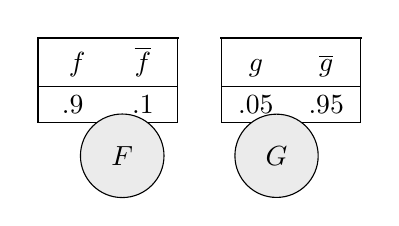
\begin{tikzpicture}[center base, scale=0.7, AmpRep]
        % \def\figtabledist{1.4}
        % \def\fignodedist{1.2}
        % \def\figtableheight{0.22}
        \def\figtabledist{0.2}
        \def\fignodedist{1.4}
        \def\figtableheight{0.41} 

        \matrix [table with head, column 1/.style={leftrule}, anchor=south east,
             column 2/.style={rightrule}, row 2/.style={bottomrule}] at (-\figtabledist,\figtableheight) {
            \vphantom{$\overline fg$} $f$ \& \vphantom{$\overline fg$}$\overline f$\\
            .9 \& .1\\
        };
        \matrix [table with head, column 1/.style={leftrule}, anchor=south west,
             column 2/.style={rightrule}, row 2/.style={bottomrule}] at (\figtabledist,\figtableheight) {
             \vphantom{$\overline fg$}$g$ \& \vphantom{$\overline fg$}$\overline g$\\
             .05 \& .95\\
        };
        \node[dpadded, circle, fill=black!08, fill opacity=1] (floomp) at (-\fignodedist,0) {$F$};
        \node[dpadded, circle, fill=black!08, fill opacity=1] (gun) at (\fignodedist,0) {$G$};
    \end{tikzpicture}
    ~~\vrule~~
	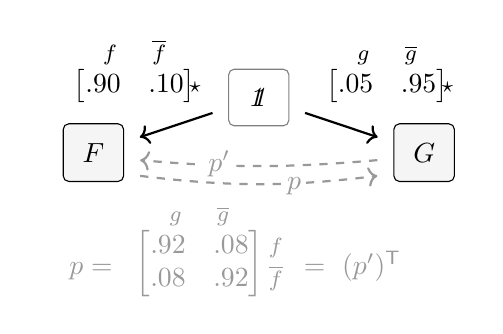
\begin{tikzpicture}[center base]

        \def\fignodedist{2.1}
        \def\fignodeheight{1.1}
        \def\newcptX{-0.3}
        \def\newcptY{-0.1}
                     
		\node[dpadded, fill=white, draw=gray] (true)  at (0,1.8) {$\pdgunit$};
		\node[dpadded] (floomp) at (-\fignodedist,\fignodeheight) {$F$};
		\node[dpadded] (gun) at (\fignodedist,\fignodeheight) {$G$};			
		
		\draw[arr] (true) to[bend left=0] coordinate(A) (floomp);
		\draw[arr] (true) to[bend right=0] coordinate(B) (gun);

		\node[above left=2.0em and 1.5em of A, anchor=center] {
        %oli14 fix gray.
			% \begin{idxmat}{\!\!\!$\star$\;\;\;}{$f$, $\overline f$}
			\begin{idxmat}[\color{black}\smalltext]{\!\!\!$\star$\;\;\;}{$f$, $\overline f$}
				.90 & .10 \\
			\end{idxmat}
		};
		\node[above right=2.0em and 1.3em of B, anchor=center] {
        %oli14
        % \begin{idxmat}{\!\!\!$\star$}{$g$, $\overline g$}
			\begin{idxmat}[\color{black}\smalltext]{\!\!\!$\star$}{$g$, $\overline g$}
				.05 & .95 \\
			\end{idxmat}
		};
		\definecolor{heldout}{rgb}{0.6, 0.6, .6}	
		\draw[heldout, dashed, arr] (floomp.-30) to[bend right=7] node[pos=0.65, fill=white, inner sep=2pt] (C) {$\smash{p}\vphantom{v}$} (gun.210);
        %oli12: addes reverse arrow, edited the above line with a yshift.
        \draw[heldout, dashed, arr] (gun.190) to[bend left=5] node[pos=0.668, fill=white, inner sep=2pt] {$\smash{p'}\vphantom{v}$} (floomp.-10);
		\node[anchor=center] (newcpd) at (\newcptX,\newcptY) {
			\color{heldout}
	%oli26: [reviewer #3] wants to unify the fonts.
	% I had wanted the bold for the matrix representation, but this
	% is not clear from context and it's not worth introducing this. 
	% It's a little bit of an abuse of notation to use matrices for cpds
	% but it's not really that bad, and it's a graphical depiction anyway.
	% Therefore I'm removing the bold here.
		% $\mat p
		$p
			=\!\!\!$\begin{idxmat}[\color{heldout}\smalltext]{$f$,$\overline f$}{$g$, $\overline g$}
%joe12
%			  .92 & 0.08 \\ .08 & .92 \\
			  .92 & .08 \\ .08 & .92 \\
          \end{idxmat}$~=~
	%oli26: ... and here also (also adding parens to make transpose clear).
		% {\mat p'^{\textsf T}}$
		    {(p')^{\textsf T}}$
		};
        % \node[below=3pt of newcpd] {\color{heldout}$\mat p' = \mat p^{\textsf T}$};
	\end{tikzpicture}
	}
\fi
    %oli12 update caption accordingly.
    %oli12: note before editing caption: making it fit on one line is not easy.
	% \caption{An inconsistent PDG, requiring resolution}
%joe11
%        \caption{A BN (left), and respective PDG (right), which can
%oli19: added word "simple" BN
%joe17: why did you add it?  What is a simple BN?
%oli20: Nothing technical. It doesn't look very much like a BN and I
%wanted to assure  
% readers that nothing strange is going on here. I trust your judgement and gether you
% think it's negative, and so am pre-emptively reverting it.
        \caption{A BN (left) and corresponding PDG (right), which can
        include more cpds; $p$ or $p'$ make it inconsistent.} 
    \label{fig:gun-floomp-diagram}
\end{figure}


%oli12
% Now suppose that you later discover that
A traumatic experience a few hours later leaves Grok believing that
%joe11
%``floomp'' is likely (92\%) to be another word for gun.
``floomp'' is likely (probability .92) to be another word for gun.
%oli12: I've removed the directionality by adding arrows in both directions.
%, and come to believe that if floomps are legal (resp., illegal), then
% there's a  chance guns are as well, and vice versa. 
%joe7: r seems like a atrange letter to use, although it's not a big deal
%oli12: I don't care about the letter. let's use p? Also this notation, while 
% you might not like it, is the consensus, especially in the conference we're 
% submitting to. We're already giving them something quite out of the ordinary;
% I don't want  to push it too far.  It's also expedient here as it lets us 
% immediately indicate the direction.
Let $p(G \mid F)$ be the \emph conditional \emph probability \emph
distribution (cpd) that describes 
the belief that if floomps are legal (resp., illegal),
%joe11
%then with 92\% probability, guns are as well, and $p'(F \mid G)$ be
then with probability .92, guns are as well, and $p'(F \mid G)$ be
the reverse. 
%oli12:
% A first reaction might be to
Starting with $p$, Grok's first instinct is to
simply incorporate the conditional information by adding $F$ as a parent of
$G$, and then associating
the cpd
$p$ with $G$. But then what should she do
with the original probability she had for $G$?  Should she just discard it?
It is easy to check that there is no 
%oli12
% probability distribution 
joint distribution
that is consistent with
%oli12 inserted
both
the two original priors on $F$ and $G$ and also 
%oli12: already lots of commas in this sentence. saying "the cpd" too often also gets to be a lot....
%the cpd $\mat r$, so if she
%joe11
%$p$---so if she
$p$.  So if she
is to represent the information with a BN, which always represents a consistent
distribution, she must resolve the inconsistency. 





However,
%oli12: rewrote paragraph.
% it may be better not to sort this out right away. 
% How to resolve it may be clearer 
% if you can get confirmation that guns are indeed floomps, or read the
% laws more carefully.
sorting this out immediately may not be ideal.
For instance, if the inconsistency arises from a conflation between
two definitions 
of ``gun'', a resolution will have destroyed the original cpds. A
better use of computation may be to notice the inconsistency and look
up the actual law. 

By way of contrast, consider the corresponding PDG. In a PDG, the cpds are
attached to edges, rather than nodes of the graph.
%oli12: this discussion is a distraction; it has nothing to do with PDGs over BNs.
 % we don't mention matrices anywhere else anymore, and the matrix representation
 % in the figure is both a common and inutuitive way of describing this
%
% The cpd associated with an
% edge $e$ from $X$ to $Y$ is a matrix $\mat e$, where the element $\mat e_{x,y}$
% at row $x$ and column $y$ is the conditional probability $\Pr(Y \!\!=\!\!y \mid
% X \!\!=\!\! x)$. 
In order to represent unconditional probabilities, we introduce
%joe25: I can't distinguish \pdgunit from a regular 1.  Can we use a
%different font or symbol for this variable?
%oli27: I'm happy to do this but could not come up with a font/symbol
% I like on the spot. Let me know if you have suggestions; I'll think about
% it while you do your pass. 
%joe26: some thoughts: U in some special font
a \emph{unit variable} $\pdgunit$ which 
%oli12: no reason to be too verbose here; more important stuff is coming.
% takes on only one possible value, which we denote
takes only one value, denoted
$\star$. 
%oli12: Thus, we have
This leads Grok to 
the PDG depicted in \Cref{fig:gun-floomp-diagram},
where the edges from $\pdgunit$ to $F$ and $G$ are associated with the
unconditional probabilities of $F$ and $G$, and the 
%oli12
%edge from $F$ to $G$ is associated with the cpd $p$. 
edges between $F$ and $G$ are associated with $p$ and $p'$.



%joe11: if we make everything black, we should get rid of ``black'' in
%the next line.
The original state of knowledge consists of all three nodes and the two
%oli13: the important bit is that they're solid. I'm trying to
%linguistically  exclude the blue/ dashed lines.
% black
solid
edges from $\pdgunit$. This is like Bayes Net that we considered above,
%joe11
%except we
except that we 
no longer
%oli12! 
explicitly
%joe11
%oli13:  :(  I think "to be" sounds way better. It's shorter, it doesn't expend
% our limited supply of "and", "that" and "are", which tiring quickly. It sounds
% cooloer. That's also definitely how I would say it in person; I
% think the "that 
% ... are" sounds like you're talking to someone you only trust to know simple 
% grammar --- but in fact, "to be" often taught earlier when people learn English
% as a foreign language, so this form is shorter and without an accesibility 
% cost.
% I believe the infinitive also strengthens the statement by not implying a 
% present tense (how is time relevant here?). I'm changing it back. If you have 
% a reason for your aesthetic preference that you think objectively outweighs this
% consideration to a significant degree, you can change it back and I will 
% accept it without argument, but ask you why later.
%
% assume that $F$ and $G$ are independent; we merely record the constraints
%joe12: if you must have ``to be''
%assume $F$ and $G$ to be independent; we merely record the constraints
take  $F$ and $G$ to be independent; we merely record the constraints
imposed by the given probabilities.  
	
The key point is that we can incorporate the new information into our original
representation (the graph in \Cref{fig:gun-floomp-diagram} without the edge from
$F$ to $G$) simply  by adding the edge from $F$ to $G$ and the associated cpd
%joe12: I could accept that the new information is in gray but then
%why are f and \overline{f}, g nad \overline{g}, and * in gray?
%oli14: Fixed. The reason is because I didn't want to draw focus towards the labels.
%$\mat r$. Doing so does not change the meaning of the original edges.  
%oli14:
% $\mat p$ (the new infromation is shown in gray). 
$p$ (the new infromation is shown in blue).
Doing so does not change the meaning of the original edges.   
%oli12: redundant.
% This
% presentation lets us simply include information, and resolve inconsistencies
% later.
Unlike a Bayesian update, the operation is even reversible: all we need
to do recover our original belief state is delete the new edge, 
%oli12: no need for 'effectively'
%effectively
making it possible to mull over and then reject an observation.
%
\end{example}


The ability of PDGs to model inconsistency, as illustrated in
\Cref{ex:guns-and-floomps}, appears to have come at a significant cost. We seem
to have lost a key benefit of BNs: the ease with which they can
capture
%joe20: it seems strange to say ``Pearl has argued'', and then
%reference a paper by Pearl, Geiger, and Verma
%(conditional) independencies, which, as Pearl \cite{pearl1989conditional} has
(conditional) independencies, which, as Pearl (\citeyear{pearl}) has
argued forcefully, are omnipresent.
%oli12*: it seems like we should add a sentence fragment here, along
%the lines of "but we will be able to easily recover them".  Also, the
%above is kind of redundant, so I keep looking at it trying to figure
%out how to re-word, but it's so well written that I can't figure out
%what I want to do to it.
%joe11: how about:
%As we shall see, we will be able to recover this information.
%oli13: Most anything we add without cutting down the text before will
%ultimately cost a line. I'm not sure this particular phrase is worth
%it, I've commented it out. 
% Counterproposal:
%joe12: Looks like you didn't finish this here
%joe13*: you still didn't finish this sentence.  I'm cutting it.
%And yet:
%oli15: The intention was to lead directly to the example. It's a
%clever but maybe  
% too-cute transition; it is free (fits on on the line) if you remove a comma. 


% most of the time, we do not make the independence
% assumption in a bn because we know for certain that the
% variables are independent; rather, we just suspect that the
% identified edges are by much more important than the
% others. determining for sure that smoking  and second hand
% smoke are independent, controlling for parents' smoking
% habits, would extremely difficult, and would require
% empiricism to validate. 


\begin{example}[emulating a BN]\label{ex:smoking}

We now consider the classic (quantitative) Bayesian network $\cal B$, which has
four binary variables indicating whether a person ($C$) develops cancer, ($S$)
smokes, ($\mathit{SH}$) is exposed to second-hand smoke, and ($\mathit{PS}$) has
parents who smoke, presented graphically in \Cref{subfig:smoking-bn}. We now
walk through what is required to represent $\cal B$ as a PDG, which we call
$\PDGof{{\mathcal B}}$, shown as the solid nodes and edges in
\Cref{subfig:smoking-pdg}. 


%oli24: To make the figure appear in the rigght place, we have to move it to
% be way earlier. Also, some magic \hfils to center it more appropriately...
\begin{figure}[ht!]
\addtocounter{figure}{1}
\centering
\hfill
%oli24: tikzexternalize doesn't work on these...
% \begin{tikzcd}[center base, column sep=1.0em, row sep=0em, dpad={fill opacity=1,fill=black!08, circle, inner sep=3pt, minimum size=2.3em, draw=gray}, 
% 	ampersand replacement=\&]
% \& S \ar[dr] \\
% PS \ar[ur]\ar[dr] \&\& C \\
% \& SH \ar[ur]
% \end{tikzcd}
% }
% \caption{The Bayesian network $\cal B$}
\ifprecompiledfigs
\raisebox{-0.5\height}{\includegraphics{figure-pdfs/smoking-BN}}
% \raisebox{-0.5\height}{\includegraphics{smoking-BN}}
\else
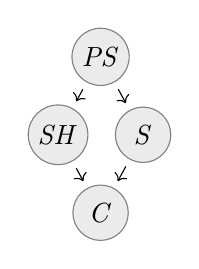
\begin{tikzpicture}[paperfig]
	\begin{scope}[every node/.style={dpadded, fill opacity=1,fill=black!08, circle, inner sep=2pt, minimum size=2em, draw=gray}]
		\node (PS) at (0,1.1) {$\mathit{PS}$};
		\node (SH) at (-0.6,0) {$\mathit{SH}$};
		\node (S) at (0.6,0) {$\mathit{S}$};
		\node (C) at (0,-1.1) {$\mathit{C}$};
	\end{scope}
	\draw[->] (PS) to (S);
	\draw[->] (PS) to (SH);
	\draw[->] (SH) to (C);
	\draw[->] (S) to (C);
\end{tikzpicture}
\fi
\refstepcounter{subfigure}
\label{subfig:smoking-bn}
~~\vline~~
\ifprecompiledfigs
\raisebox{-0.5\height}{\includegraphics{figure-pdfs/smoking-PDG}}
% \raisebox{-0.5\height}{\includegraphics{smoking-PDG}}
\else
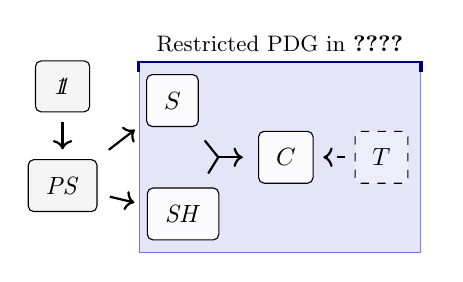
\begin{tikzpicture}[paperfig]
	\fill[fill opacity=0.1, blue!80!black, draw, draw opacity=0.5] (2.73,1.35) rectangle (6.7, -1.35);
	
	%oli24: modifying positions to fit things...
	% \node[dpadded] (1) at (0,0) {$\pdgunit$};
	% \node[dpadded] (PS) at (1.65,0) {$\mathit{PS}$};
	\node[dpadded] (1) at (1.65,1) {$\pdgunit$};
	\node[dpadded] (PS) at (1.65,-0.4) {$\mathit{PS}$};
	\node[dpadded, fill=black!.16, fill opacity=0.9] (S) at (3.2, 0.8) {$S$};
	\node[dpadded, fill=black!.16, fill opacity=0.9] (SH) at (3.35, -0.8) {$\mathit{SH}$};
	\node[dpadded, fill=black!.16, fill opacity=0.9] (C) at (4.8,0) {$C$};
	
	\draw[arr1] (1) -- (PS);
	\draw[arr2] (PS) -- (S);
	\draw[arr2] (PS) -- (SH);
	\mergearr{SH}{S}{C}
	
	\node[dpadded, fill=black!.16, fill opacity=0.35, dashed] (T) at (6.15,0) {$T$};
	\draw[arr1,dashed] (T) -- (C);	

	\draw[very thick, |-|, color=blue!50!black,text=black] (2.7, 1.35) --coordinate(Q) (6.73,1.35);%(7.13,1.35);
	\fill[white] (2.6, 1.36) rectangle (6.9,1.55);
	% \useasboundingbox (current bounding box);
	\node[above=0.05em of Q]{\small Restricted PDG in \cref{ex:grok-ablate,ex:grok-union}};
\end{tikzpicture}
\fi
	\hfill~
%oli12: I wasn't really sure what to do with this caption given that it really needs to be 2/3 of a line for the figure to look right.
% \caption{The PDG $\PDGof{{\mathcal B}}$ corresponding to ${\mathcal B}$, and a restriction of it.} 
% \caption{The PDG $\PDGof{{\mathcal B}}$, and two alterations of it.} 
	\refstepcounter{subfigure}
	\label{subfig:smoking-pdg}
\addtocounter{figure}{-1}
% \end{subfigure}
%oli24*: merging captions together + updating them. SUbfigures are a bother with AAAI...
% \caption{Graphical models representing conditional relationships in \Cref{ex:smoking,ex:grok-ablate,ex:grok-union}}
\caption{ (a) The Bayesian Network $\mathcal B$ in \cref{ex:smoking} (left), and
(b) $\PDGof{\mathcal B}$, its corresponding PDG (right). The shaded box
indicates a restriction of $\PDGof{\mathcal B}$ to only the nodes and edges it
contains, and the dashed node $T$ and its arrow to $C$ can be added in the PDG,
without taking into account $S$ and $SH$.}
\label{fig:smoking-bn+pdg}
\end{figure}

We start with the nodes corresponding to the variables in $\cal B$, together
%joe26: changed \sf 1 to \pdgunit, so that you change all occurrences
%with the special node $\sf 1$ from \Cref{ex:guns-and-floomps}; we add an edge
%from ${\sf 1}$ to $\mathit{PS}$, to which we associate the unconditional
with the special node $\pdgunit$ from \Cref{ex:guns-and-floomps}; we add an edge
from ${\pdgunit}$ to $\mathit{PS}$, to which we associate the unconditional
probability given by the cpd for $\mathit{PS}$ in $\cal B$. We can also re-use
the cpds for $S$ and $\mathit{SH}$, assigning them, respectively, to the edges
$PS \to S$ and $PS \to SH$ in $\PDGof{{\mathcal B}}$.
There are two remaining problems: (1) modeling the remaining table in $\cal B$,
which corresponds to the conditional probability of $C$ given $S$ and $SH$; and
(2) recovering the additional
%oli12 added
conditional
independence assumptions in the BN. 

For (1), we cannot just add the edges $S \to C$ and $SH \to C$ that are present
%joe11: line shaving
%in $\cal B$, because, as we saw in \Cref{ex:guns-and-floomps}, this would mean
in $\cal B$. As we saw in \Cref{ex:guns-and-floomps}, this would mean
supplying two \emph{separate} tables, one indicating the probability of $C$
given $S$, and the other indicating the probability of $C$ given
%joe11: more line shaving
%$\mathit{SH}$. Doing this would lose significant information that is
$\mathit{SH}$.  We would lose significant information that is
present in $\cal B$  about 
how $C$ depends jointly on $S$ and $SH$. To distinguish the joint dependence on
$S$ and $\mathit{SH}$, for now, we draw an edge with two tails---a
%oli26: [reviewer #5]: confused that hyper-edges are usually undirected. insert:
(directed)
\emph{hyperedge}---that completes the diagram in \Cref{subfig:smoking-pdg}. 
%
With regard to (2), there are many distributions consistent with the conditional
marginal probabilities in the cpds, and the independences presumed by $\cal B$
need not hold for them. 
%oli12
% Rather than encoding the extra probabilistic information as cpds,
Rather than trying to distinguish between them with additional constraints,
we develop a a scoring-function semantics for PDGs
%oli12: hmm, the consistency is part of the scoring function. 
%    , and show that, among all distributions consistent with
%    $\PDGof{{\mathcal B}}$,
%joe11: so we're encoding the constraints in the semantics of the
%scoring function, rather than directly in the PDG.  This makes it a
%``soft'' constraint.  We could say that somewhere, but this seems
%like the wrong place.
%joe11: I don't know what ``emphasis on matching (potentially
%arbitrary) cpds'' means 
%which, despite an emphasis on matching (potentially arbitrary) cpds,
which 
is in this case uniquely minimized by the distribution 
%joe8*: I think we need to throw out hints about how we're going to
%use scoring functions.  I view this as critical
%oli12: I think the BN result is strong enough that this is too much hedging.
% for the appropriate scoring function, 
% the unique distribution with a minimum
% score is the one
%
specified by ${\mathcal B}$ (\Cref{thm:bns-are-pdgs}).
This allows us to recover the semantics of Bayesian networks without requiring the independencies that they assume.

%But now suppose that we get information beyond that captured by the
Next suppose that we get information beyond that captured by the original BN.
Specifically, we read a thorough empirical study demonstrating that people who
use tanning beds have a 10\% incidence of cancer, compared with 1\% in the
%oli26 [reviewer #3]: "control what?"
% control 
control group 
(call the cpd for this $p$); we would like to add this information to
$\cal B$. The first step is clearly to add a new node labeled $T$, for ``tanning
bed use''.  But simply making $T$ a parent of $C$ (as clearly seems appropriate,
given that the incidence of cancer depends on tanning bed use) requires a
substantial expansion of the cpd; in particular, it requires us to make
assumptions about the interactions between tanning beds and smoking.  
%
The corresponding PDG, $\PDGof{{\mathcal B}}$, on the other hand, has no
trouble: We can simply add the node $T$ with an edge to $C$ that is associated
with $\mat p$.  But note that doing this makes it possible for our knowledge to
be inconsistent. To take a simple example, if the distribution on $C$ given $S$
and $H$ encoded in the original cpd was always deterministically ``has cancer''
for every possible value of $S$ and $H$, but the distribution according to the
new cpd from $T$ was deterministically ``no cancer'', the resulting PDG would be
inconsistent.  
%
\end{example}


We have seen that we can easily add information to PDGs; removing information is
equally painless.   

\begin{example}[restriction]\label{ex:grok-ablate}
%oli12
% After the communist uprising, 
%joe11
%  After the communist party came to power,
  After the Communist party came to power,
  children were raised communally, and so parents' smoking habits no longer had any impact on them. Grok is reading her favorite book on graphical models, and she realizes that while the node $\mathit{PS}$ in \Cref{subfig:smoking-bn} has lost its usefulness, and nodes $S$ and $\mathit{SH}$ no longer ought to have $\mathit{PS}$ as a parent, the other half of the diagram---that is, the node $C$ and its dependence on $S$ and $\mathit{SH}$---should apply as before.
%oli4: this next sentence is less useful, and can be
    %removed; its purpose is to pre-emptively push against
    %a desire to margnialize and get a new BN.  
%joe4: let's remove it
% \begin{edge} 
% 	The rise of the communist party also came with changes in smoking habits, so a new unconditional distribution on $S$ could not be obtained by eliminating the variable $PS$. 
% \end{edge}
Grok has identified two obstacles to modeling deletion of information from a BN
by simply deleting nodes and their associated cpds. First, this restricted model
is technically no longer a BN (which in this case would require unconditional
distributions on $S$ and $\mathit{SH}$), but rather a \emph{conditional} BN
\cite{KF09}, which allows for these nodes to be marked as observations;
observation nodes do not have associated beliefs. Second, even regarded as a
conditional BN, the result of deleting a node may introduce \emph{new}
independence information, incompatible with the original BN. For instance, by
deleting the node $B$ in a chain $A \rightarrow B \rightarrow C$, one concludes
that $A$ and $C$ are independent, a conclusion incompatible with the original BN
containing all three nodes.   
%joe7*: shortened significantly.  I don't think it's
   %worth agonizing this over this.
%oli12: Your shortening is excellent :)
%joe11: :-)
PDGs do not suffer from either problem.  We can easily delete the
nodes labeled 1 and $PS$ in \Cref{subfig:smoking-pdg} to get the
restricted PDG shown in the figure, which captures Grok's updated information.
%oli12: I want to keep some of the material  underneath it for the
%full paper though. 
% I have rewritten a lot of it.
%joe17: I can live with this in the paper
%\begin{vfull}
The resulting PDG has no edges leading to $S$ or $\mathit{SH}$, and hence no
distributions specified on them; no special modeling distinction between
observation nodes and other nodes are required. Because PDGs do not directly
make independence assumptions, the information in this fragment is truly a
subset of the information in the whole PDG. 	
%\end{vfull}
% 
\end{example}

Being able to form a well-behaved local picture and restrict knowledge is
useful, but an even more compelling reason to use PDGs is their ability to
aggregate information. 
	
\begin{example}\label{ex:grok-union}
Grok dreams of becoming Supreme Leader ($\it SL$), and has come up with a plan.
She has noticed that people who use tanning beds have significantly more power
%oli26: [reviewer #3] "no and"
% and than those who don't. Unfortunately, her mom has always told her that
than those who don't. Unfortunately, her mom has always told her that tanning
beds cause cancer; specifically, that 15\% of people who use tanning beds get
it, compared to the baseline of 2\%. Call this cpd $q$. Grok thinks people will
make fun of her if she uses a tanning bed and gets cancer, making becoming
Supreme Leader impossible. This mental state is depicted as  a PDG on the left
of \Cref{fig:grok-combine}.

Grok is reading about graphical models because she vaguely remembers that the
variables in \Cref{ex:smoking} match the ones she already knows about. When she
finishes reading the statistics on smoking and the original study on tanning
beds (associated to a cpd $\mat p$ in \Cref{ex:smoking}), but before she has
time to reflect, we can represent her (conflicted) knowledge state as the union
of the two graphs, depicted graphically on the right of \Cref{fig:grok-combine}.  


\begin{figure}
	\hfill
	\ifprecompiledfigs
%oli25: resetting all of these (I'm only marking %oli25 here), though
% I'll leave the other version commented out just in case. I believe 
% I fixed the flags so that I'm the only one who has to worry about this.
\raisebox{-0.5\height}{\includegraphics{figure-pdfs/grok-pre}}
% \raisebox{-0.5\height}{\includegraphics{grok-pre}}
\hspace{1.2em}\vline\hspace{1.2em}
\raisebox{-0.5\height}{\includegraphics{figure-pdfs/grok-post}}
% \raisebox{-0.5\height}{\includegraphics{grok-post}}
	\else
	\colorlet{colorsmoking}{blue!50!black}
	\colorlet{colororiginal}{orange!80!black}
	\tikzset{hybrid/.style={postaction={draw,colorsmoking,dash pattern= on 5pt off 8pt,dash phase=6.5pt,thick},
		draw=colororiginal,dash pattern= on 5pt off 8pt,thick}}
	\centering
	\begin{tikzpicture}[paperfig, thick, draw=colororiginal, text=black]
		\node[dpadded] (C) at (0,0) {$C$};
		\node[dpadded] (T) at (2,0){$T$};
		\node[dpadded] (SL) at (1,-1.5){$\it SL$};
		
		\draw[arr] (T) to[bend right] node[above]{$q$} (C);
		\mergearr{C}{T}{SL}
	\end{tikzpicture}
	\hspace{1.6em}\vline\hspace{1.6em}
	\begin{tikzpicture}[paperfig]
		\begin{scope}[postaction={draw,colorsmoking,dash pattern= on 3pt off 5pt,dash phase=4pt,thick}]
			
			\node[dpadded,hybrid] (C) at (0,0) {$C$};
			\node[dpadded,hybrid] (T) at (2,0){$T$};
		\end{scope}
		
		\begin{scope}[thick, draw=colororiginal, text=black]
			\node[dpadded] (SL) at (1,-1.5){$\it SL$};
			\draw[arr] (T) to[bend right] node[above]{$q$} (C);
			\mergearr{C}{T}{SL}
		\end{scope}


		\begin{scope}[thick, draw=colorsmoking, text=black]
			\node[dpadded] (S) at (-1.4, 0.8) {$S$};
			\node[dpadded] (SH) at (-1.45, -0.8) {$\mathit{SH}$};
			\draw[arr] (T) to node[fill=white, fill opacity=1,text opacity=1,inner sep=1pt]{$p$} (C);
			\mergearr{S}{SH}{C}
		\end{scope}
	\end{tikzpicture}
	\fi
	\hfill~
	\caption{Grok's prior (left) and combined (right) knowledge.}
	\label{fig:grok-combine}
\end{figure}

The union of the two PDGs, even with overlapping 
%oli24:
% nodes and is still a PDG.
nodes, is still a PDG.
This is not the case in general
%oli24:
% with a BN.
for BNs.
Note that the PDG that Grok used to
represent her two different sources of information (the mother's wisdom and the
study) regarding the distribution of $C$ is a \emph{multigraph}: there are two
edges from $T$ to $C$, with inconsistent information.
%oli26 [reviewer #3] "something wrong in text here" --- I think deleting
% one of the "nots" is enough? I'm also changing the tense to past perfect.
%% Had we not not allowed multigraphs, we would need to choose between the two edges, or represent the
Had we not allowed multigraphs, we would have needed to choose between the two edges, or represent the
information some other (arguably less natural) way. As we are already allowing
inconsistency, merely recording both is much more in keeping with the way we
have handled other types of uncertainty. 
%		
%TODO: I should not say this yet. This is a related story that I haven't told yet. 
%Moreover, if Grok were to later discover that her mother had been faithfully transmitting the results of an unrelated study, she would be justified in increasing her certainty that a cpd roughly like $\mat p$ and $\mat q$ were correct.
% This suggests a result that is perhaps obvious in retrospect: the mere \emph{possibility} of inconisistency increases the value of consistency. For an agent that is guaranteed to be consistent by design, corroborating evidence has no value. 
\end{example}

Not all inconsistencies are equally egregious. For example, even though the cpds
$p$ and $q$ are different, they are numerically close, so, intuitively, the PDG on the right in
\Cref{fig:grok-combine} is not very inconsistent.
Making this precise 
%oli12:  
% will be
is
the focus of \Cref{sec:scoring-semantics}.


%joe4*: While I don't have an intrinsic problem with this paragraph,
%I'm not sure it belongs in the introduction.  Do we discuss this in
%more detail elsewhere in the paper?   If so, we have to say more
%about it.  As it stands, it seems like a letdown, after quite a
%compelling introduction.  I cut it for now.
%
%oli5: I agree with your assessment that it either needs to be followed
% up by something, or removed---although I'm not sure I agree there needs
% to be more text here. I strongly prefer to follow it up with something;
% I think path composition is one of the most important selling point of PDGs, 
% on par with the ability represent inconsistency, and showcases
% modularity in a useful, compositional way. To reflect this preference,
% I'm uncommenting this, but you're welcome to re-comment it in the next iteration.
%joe5*: commenting out, until you come up with a story for it that
%fits in the paper.  I strongly suspect that it won't make it into a
%NIPS submission, so by commenting it out, we'll be able to better
%judge space.
\commentout{
While a PDG is in some sense merely a set of constraints (the cpds), these constraints themselves have a useful computational meaning. Regarding cpds as stochastic matrices, we can get cpds corresponding to paths by multiplying them; equivalently, thought of as probabilistic functions, we can compose them.
	For instance, in \Cref{ex:grok-union}, if we were to give Grok
        unconditional probabilities in the form of vectors
        $\smash{(\vec s, \vec h, \vec t)}$ over the possible values of
        $\mathit{S, SH}$ and $\mathit T$ respectively, she could
        compute three distinct estimates for $\mathit{SL}$. This is
        perhaps clearest visually, but for clarity, if $\mat S$ is
        the cpd for the orange hyperedge that computes $C$ from
        $\mathit{S, SH}$, and $\mat L$ is the cpd for the
%joe4: the colors may not come across for some people, so you may want
%to use some other way of distinguishing them
%oli5*: Can I rely on colors to distinguish things in general? I've been using it throughout the document. I've seen papers that do this, but I can see why it might be poor taste (e.g., black and white printers). I can add letters to the hyper-edges here.
%        blue hyper edge, which computes $\mathit{SL}$ from $\mathit{C, T}$, and
%        $[\vec a; \vec b]$ is a vertical stacking of the vectors $\vec
    blue hyperedge that computes $\mathit{SL}$ from $\mathit{C, T}$, and we 
%oli5:
% use the notation 
		write
        $[\vec a; \vec b]$ for the matrix with rows $\vec
        a$ and $\vec b$, then 
	\[ \mat L \Big[\mat p \vec t; \vec t\ \Big],
		\qquad \mat L \Big[\mat q \vec t; \vec t\ \Big], \quad\text{and}
		\quad \mat L \Big[\mat S \big[\vec s; \vec h\big], \vec t\ \Big]  \]
	        are all probabilistic estimates of $\mathit{SL}$, which
                can be used in different circumstances: the first two are
        applicable even if given only $\vec t$, and the last requires
        all three values. 
	This property gives PDGs more useful structure than most
        collections of constraints.  
}
%joe5: \end{commentout}
        
These examples give a taste of the power of PDGs.  In the coming sections, we formalize PDGs and relate them to other approaches.		
% \begin{notfocus}
%	\begin{enumerate}[nosep]
%		\item This representation more naturally matches what humans are aware of, encoding small locally consistent models rather than one giant probability distribution
%		\item It is a strictly more general representation--- we can easily convert BNs to these diagrams (section \ref{sec:convert2bn})
%		\item This allows composition of arrows to be defined, and gives meanings to paths (section \ref{sec:composition}).
%		\item Allowing variables to be added and removed makes
%		\item Changing and partially determining arrows is more reasonable.
%		\item We can now represent inconsistency, which will allow us to capture mental states which, and . While we agree with the classical picture in that inconsistency is bad, now we can talk about it
%	\end{enumerate}
% Redundency is important: types in programming languages, more data in ML systems.
% Puts gurads
% Makes it possible to combine knowledge without destroying old knowledge.
% preference updating
	
	
\section{Syntax}\label{sec:formal+syntax}
We now provide formal definitions for PDGs.        
Although it is possible to formalize PDGS with hyperedges directly,
    we opt for a different approach here, in which PDGs have only regular edges,
and hyperedges are captured using a simple construction
that involves adding an extra node.

\vfull{\footnote{In the factor graph literature,
          especially with regard to loopy belief propagation
          \cite{wainwright2007graphical}, it is common to
          call a collection of marginals that are not
          necessarily all compatible with a distribution
          \emph{pseudomarginals}, making a PDG in some sense a
          collection of `conditional' pseudomarginals. This
          gives an alternate, more technically precise
          expansion of PDG as ``Pseudomarginal Dependency Graph''.}}

%oli22: removing label for line shave
% \begin{defn}[PDG]\label{def:model}
\begin{defn}\label{def:model}
%oli22: editing so that I can explicitly get graph, modified from 
% DN-and-WFG.tex as per our discussion.
% A \emph{Probabilistic Dependency Graph} is a tuple $\pdgvars[]$ where
%joe20*: reverted back to previous version.  I tried to salvage what
%you did below, but I'm really unhappy about this
%A \emph{Probabilistic Dependency Graph} is a tuple $\dg M = (\Gr,\mat
A \emph{Probabilistic Dependency Graph}
%oli24: \E was expectation (changed to \Ex to avoid confusion) and \Ed is edges. 
%oli24: also, the \alpha, \beta didn't get swapped. 
% is a tuple $\dg M = (\N,\E,\V,\mat p, \beta,\alpha)$, where 
is a tuple $\dg M = (\N,\Ed,\V,\mat p, \alpha, \beta)$, where 

%oli22: I still think ((\N,\V), E) is better notation, because it 
% is of the form ( VERT , E ) where VERT = (\N,\V) is the data necessary 
% to specify the variables (the vertices of the graph), and  E is a set of edges
% like usual. In other points we also want to refer to the set of variables, 
% which I have been writing (\N, \V). Do you think what I have below is better?
%joe20*: I *strongly* disagree.  A multigraph is a standard notion.
%You shouldn't change standard definitions.  We had agreed that you
%wouldn't do this.  Please do not do what we had agreed you wouldn't
%do without discsussing it.  It creates extra work for me and extra
%work for you.  I find this completely unacceptable.
%$\Gr = (\N,\Ed,\V)$ is a multi-graph whose nodes are variables, while
%$\Gr = (\N,\Ed)$ is a multi-graph whose nodes are variables, while
%$\Gr = (\N,\Ed)$ is a multi-graph whose nodes are variables, while
%$\mat p,\beta,\alpha$ respectively give a cpd and two weights
% its reliability,
%for each edge in $\Ed$. More precisely,
%
\begin{description}%[nosep]
	\item[$\N$] \notation{$:\Set$}%
		is a finite set of nodes, corresponding to variables;
	\item[$\Ed$] \notation{$\subseteq \N \times \N \times \mathit{Label}$}%
%oli22: clarify "arbitrary", introduce notation, and pull focus away from 
% the label, which is a necessary technicality. 
%Question: With the arrow,  "source", and "target" is the word "directed" positive or negative?
		% is a set of directed edges, each with a source and target in $\N$, 
		% as well as an arbitrary label;
		is a set of labeled edges $\{ \ed LXY \}$, each with a source 
%oli24:
		% $X$ and target $Y$ in $\N$, 
		$X$ and target $Y$ in $\N$;
	\item[$\V$] \notation{$\N \to \mathbf{Set}$}%
		associates each variable $N \in \N$ with a set $\V(N)$ of values that the variable $N$ can take;
  	\item[$\mat p$] \notation{$:\big(\!({A,B,\ell})\colon\!\Ed \big) \to \V(A) \to \Delta\V(B)$}%
	% HYPERGRAPH \mat p TYPE: $\colon\!\big(\!({\bf A,B})\colon \! \Ed \big) \to \prod\limits_{A\in \bf A} \!\! \V(A) \to \underline\Delta\left[\prod\limits_{B \in \bf B}\!\!\V(B)\right]$
%oli22: introducing the name of L, use notation. The first commented line below is 
% the orignial, and the second is an option that does not use the arrow notation.
	% associates to each edge $(X,Y,\ell) \in \Ed$
	% associates to each edge $L \!=\! (X,Y,\ell) \in \Ed$
	associates to each edge $\ed LXY \in \Ed$
	a distribution $\bp(x)$ on $Y$ for each $x \in \V(X)$; 

%oli22: \alpha used to be here and I moved it below \beta.
%joe20: undid change; it's strange to have \beta before \alpha.  We
%had agreed that you wouldn't make such changes.  
\item[$\alpha$] \notation{$:\Ed \to [0,1]$}
%oli22: feel free to reinstate; see corresponding comment on \beta above
% is a function that
%oli22: replacing paragraph to correct the following:
% (1) \alpha can be zero; 
% (2) removing the semicolon and re-introduced subject for flow.
% (3) bind "X" and "Y" before reference.
% (4) remove the "agent" which we've tried so hard to avoid in the
% description of IDef, as with \beta above.
%
%  associates a non-negative real number $\alpha_L$ with each edge $L$;
%  roughly speaking, $\alpha_L$ is the agent's subjective confidence in
%  the qualitative functional dependence of $Y$ on $X$ implicit in $L$. 
%
associates to each edge $\ed LXY$ a non-negative number $\alpha_L$ which,
%joe20
%roughly speaking, is a subjective confidence in the functional
%oli24: the L all by itself is bothering me a lot visually.
% roughly speaking, is the modeler's subjective confidence in the functional
roughly speaking, is the modeler's confidence in the functional
dependence of $Y$ on $X$ implicit in $L$; 
\item[$\beta$] \notation{$:\Ed \to \mathbb R^+$}
%oli22: [should we keep "is a function"?] 
% In the body, we refer to \beta as a "vector" instead of a "function";
% also, in the definition of \mat p above, we simply say "asssociates" without
% giving either --- though perhaps it's justifiable because it's dependently 
% typed whereas this is simply a function? I have commented out "is a function"
% here and also for \alpha above, but I defer to your judgement and won't 
% follow up on this.
%joe19
% is a function that 
%oli22: swap order for consistency with other items
% associates a positive real number $\beta_L$ with each edge $L$,
associates to each edge $L$ a positive real number $\beta_L$,
%oli22: removing "agent's" to clean up definition; also removed "indicating"
% purely as a line shave.
% indicating an agent's subjective confidence in the reliability of
%joe20:
the modeler's 
subjective confidence in the reliability of
%oli22:
% the cpd $\bp$. 
%joe21
%oli27: line shave
%the cpd $\bp$;
$\bp$. 
\end{description}
%joe20: added, to try to salvage what you did.
Note that we allow multiple edges in $\Ed$ with the same source and
target; thus $(\N,\Ed)$ is a multigraph.  We occasionally write a PDG
%joe20
%as $\dg M = (\Gr,\mat p, \beta,\alpha)$, where $\Gr = (\N,\E,\V)$, and
%joe21: Note that we have three deifferent font in G-(N,E,V)
as $\dg M = (\Gr,\mat p, \alpha,\beta)$, where $\Gr = (\N,\Ed,\V)$, and
%joe21
%abuse terminology by referring to $\Gr$ as $\Gr$ as a multigraph.
abuse terminology by referring to $\Gr$ as a multigraph.
%oli22: added
%joe20: it's not a partial spefication.  
%We refer to a partial specification
We refer to 
%joe21: I think we have four different fonts here.  This is really not
%good, although I'm not going to worry about it now
%oli24: thanks for not worrying; it was an easily identifiable
% macro confusion that arose when you rewrote this bit.
${\dg N} = (\Gr, \mat p)$ as an \emph{unweighted} PDG,
%oli24: 
% pulled up from where you said this, with slight modification.
and give it semantics as though it were the (weighted) PDG $(\Gr, \mat p, \mat 1, \mat 1)$, where
$\bf 1$ is the constant function (i.e., so that $\alpha_L = \beta_L = 1$ for all $L$). 
%oli22*: We have to add \alpha_L to IDef or else the alternate
% representation of the semantics does not follow. Thus $\alph_L$ appears
% in all the places one would expect; we just don't fully discuss 
% the implications (mostly because we don't agree what they are). As a result,
% I think making too big a deal out of its lack of presense is a mistake.
%oli22: Original: 
%	Throughout most of this paper, we do not mention $\alpha_L$,
%	implicitly taking $\alpha_L\!=1$ for all edges $L$.
%oli22: this last statement seems out of place in the definition itself;
% is it important enough to re-insert afterwards?
%	(The one place where we use $\alpha_L$ is in our discussion of ...)  
%
% < various rewrites >
% In this paper, we try to avoid mentioning we implicitly take $\alpha_L=1$ for all edges $L$,  
% and abbreviate $\dg M = (\Gr, \mat p, \beta)$.
%
%joe21
%In this paper, we generally take $\alpha_L$ to equal 1 for all edges
%oli24
% In this paper, we generally take $\alpha = {\bf 1}$,
In this paper, with the exception of \cref{sec:expfam},  we implicitly take $\alpha = {\bf 1}$
% In this paper, we take $\alpha = {\bf 1}$ except in \cref{sec:expfam},
%oli24: I've pulled this parenthetical above
% (i.e., the constant function ${\bf 1}$, so that $\alpha_L = 1$ for all edges $L$) 
% unless we state otherwise,
%joe25
%and abbreviate $\dg M = (\Gr, \mat p, \beta)$.%
and omit $\alpha$, writing $\dg M = (\Gr, \mat p, \beta)$.%
%joe25*: the AAAI paper won't have an appendix, so perhaps we should
%refer to the full paper.  But what results do we have in the appendix
%about \alpha that aren't in the main paper?  In any case, you should
%look for all instances of ``appendix'' and change it to ``full paper''.
%oli27: done. 
%oli27: appendix -> full paper
% \footnote{The appendix gives the analogs of other results for
% arbitrary $\alpha$.}
%joe30
%\footnote{The full paper gives the analogs of other results for
%arbitrary $\alpha$.} 
\footnote{The full paper gives results for arbitrary $\alpha$.} 
% 
% We refer to 
% %joe21: I think we have four different fonts here.  This is really not
% %good, although I'm not going to worry about it now
% %oli24: thanks for not worrying; it was an easily identifiable
% % macro confusion that arose when you rewrote this bit.
% ${\dg N} = (\Gr, \mat p)$ as an \emph{unweighted} PDG,
% %oli24: 
% % pulled up from where you said this, with slight modification.
% and give it semantics as though it were the (weighted) PDG $(\Gr, \mat p, \mat 1, \mat 1)$,
\end{defn}
If $\dg M$ is a PDG, we reserve the names 
$\N^{\dg M}, \Ed^{\dg M}, \ldots$,
for the components of $\dg M$, so that we may reference one without naming them
all explicitly. We write $\V(S)$ for the set of possible joint settings of a set
$S$ of variables, and write
%oli21: unnecessarily complex:
% $\V(\dg M) := \prod_{N \in \N^\dg M} \V^{\dg M}(N)$
%joe19: I can't parse this
%$\V(\dg M) :=\V^{\dg M}(\N^{\dg M})$
%for all settings of the variables $(\N^\dg M, \V^\dg M)$%
%oli21: introduce for clarity
%which we also refer to as ``worlds''.
$\V(\dg M)$ for all settings of the variables in $\N^{\dg M}$; we
refer  to these settings as ``worlds''.
While the definition above is sufficient to represent the class of all legal
PDGs, we often use two additional bits of syntax
%oli29:
% to represent common constraints:  
to indicate common constraints:  
%joe25: shrinking
%\begin{itemize}
%    \item A special variable $\sf 1$ whose range consists of only
%    element, which 
%    we denote $\star$. It is used to represent unconditional
%    distributions, as 
%    in \Cref{ex:guns-and-floomps,ex:smoking}.  
%oli27: "onlyl"
% the special variable $\pdgunit$ whose range consists of onlyl $\star$,
%oli29:
% the special variable $\pdgunit$ whose range consists of only $\star$,
% discussed in \Cref{ex:guns-and-floomps,ex:smoking}; and
%joe28: I can live with \pdgunit
%the special variable $\pdgunit$ that has $\V(\pdgunit)=\{\star\}$
the special variable $\pdgunit$ such that $\V(\pdgunit)=\{\star\}$
from \Cref{ex:guns-and-floomps,ex:smoking}, and
%joe17* I would cut this.  As I said above, it breaks the flow and is
%unnecesary; the examles sffice
%oli20: oops, did not intend to reinsert this.
\vleftovers{
		\begin{example}\label{ex:worldsonly}
			A probability distribution $p$ over a measurable set $W$ of possible worlds is represented as 
			\begin{center}
				\scalebox{0.8}{
				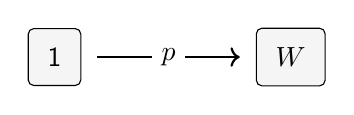
\begin{tikzpicture}
					\node[dpadded] (1) at (0,0) {$\sf 1$};
					\node[dpadded] (W) at (3,0) {$W$};

					\draw[arr] (1) to node[fill=white]{$p$} (W);
				\end{tikzpicture}}
			\end{center}
		\end{example}
}%joe17 \end{vleftovers}
%joe25
%\item Double-headed arrows, $A \tto
double-headed arrows, $A \tto B$, which visually indicate 
%joe25: it's strange to refer to a function f when the notation doesn't
%$f(a)$ for each $a \in A$ (corresponding to a deterministic
%                  function $f : A \to B$).
%oli27: somehow this got garbled: "special some element". 
% the degenerate special
% some element in $\V(B)$ for each element in $\V(A)$ (thus, effectively
% representing a deterministic function $f : A \to B$).
that the corresponding cpd is degenerate, effectively representing a deterministic
function $f : \V(A) \to \V(B)$. 
%oli27: (typesetting note: I would rather say "from \V(A) to \V(B)" but for some
% reason the entire paragaph expands and it ends up costing more than
% one line) 
%joe25
%\end{itemize}

\begin{constr}\label{constr:hyperedge-reducton}
We can now explain how we capture   the multi-tailed edges that 
were used in 
\Crefrange{ex:smoking}{ex:grok-union}. 
That notation can be viewed as shorthand for the graph that results by adding a new node at the junction representing the joint value of the nodes at the tails, with projections going back.  For instance,
% the diagram of the PDG in the shaded box of \Cref{subfig:smoking-pdg}
the diagram displaying Grok's prior knowledge in \Cref{ex:grok-union}, on the left of \Cref{fig:grok-combine}
%joe7: moved up from below, to save a line
%is really shorthand for the following PDG:
is really shorthand for the following PDG, where
where we insert a node labeled $C \times T$ at the junction:
\smallskip
	\begin{center}
	\ifprecompiledfigs
\raisebox{-0.5\height}{\includegraphics[scale=0.9]{figure-pdfs/widget}}
% \raisebox{-0.5\height}{\includegraphics[scale=0.9]{widget}}
	\else
		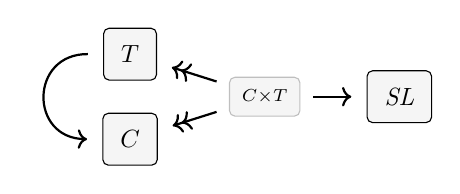
\begin{tikzpicture}[paperfig]
			\node[dpadded] (SL) at (-1.0,0) {$\mathit{SL}$};
			
			\node[dpadded,light pad] (CT) at (-2.9, 0){$\scriptstyle C \times T$};
			\node[dpadded] (C) at (-4.8, -0.6) {$C$};
			\node[dpadded] (T) at (-4.8, 0.6) {$T$};
			
	%				\node[dpadded, dashed,color=violet] (X) at (6.5,0) {$X$};
	%				\draw[arr, color=violet] (X) -- (S);
	%				\draw[arr, color=violet] (X) -- (C);
	%				\draw[arr, dashed, color=violet] (X) -- (SC);
			
			\draw[arr, ->>] (CT) -- (C);
			\draw[arr, ->>] (CT) -- (T);
			\draw[arr] (CT) -- (SL);
			\draw[arr] (T) to [bend right=90, looseness=2] (C);
	\end{tikzpicture}
	\fi
	%%%%%%%%%%%%%%%%%  smoking fragment: %%%%%%%%%%%%%%%%%%%%%%
% 		\scalebox{0.8}{
% 			\begin{tikzpicture}
% 				\node[dpadded] (C) at (-1.0,0) {$C$};
% 				\node[dpadded] (T) at (0.5,0) {$T$};
% 
% 				\node[dpadded,light pad] (SSH) at (-2.9, 0){$\scriptsize \mathit{SH} \times S$};
% 				\node[dpadded] (S) at (-4.8, 0.6) {$S$};
% 				\node[dpadded] (SH) at (-5.0, -0.6) {$\mathit{SH}$};
% 
% %				\node[dpadded, dashed,color=violet] (X) at (6.5,0) {$X$};
% %				\draw[arr, color=violet] (X) -- (S);
% %				\draw[arr, color=violet] (X) -- (C);
% %				\draw[arr, dashed, color=violet] (X) -- (SC);
% 
% 				\draw[arr, ->>] (SSH) -- (S);
% 				\draw[arr, ->>] (SSH) -- (SH);
% 				\draw[arr] (SSH) -- (C);
% 				\draw[arr] (T) -- (C);
% 		\end{tikzpicture}}
	\end{center}
	\smallskip

% That is, we inserted a node labeled $SH \times S$ at the junction.  As
% the notation suggests, $\V( \mathit{SH} \times S) = \V(\mathit{SH}) \times \V(S)$.
% The cpd for $(h,s) \in \V(\mathit{SH} \times S)$  associated with 
% the edge from $\mathit{SH} \times S$ to $\mathit{SH}$ gives probability 1 to $h$;
% similarly, the cpd for $(s,c)$  associated with 
% the edge from $ C \times C$ to $S$ gives probability 1 to $s$.
%joe7
%        That is, we inserted a node labeled $C \times T$ at the junction.
As the notation suggests, $\V( C \times T) = \V(C) \times \V(T)$.
%joe2: this is not the time to start talking about matri\mathit{SL}es
%Thus, $\V(S \times \mathit{SL}) = \V(S) \times \V(\mathit{SL})$; the matrix asso\mathit{SL}iated with
For any joint setting $(c,t) \in \V(C \times T)$ of both variables, the cpd for
the edge from $C \times T$ to $C$ gives probability 1 to $c$;
similarly, the cpd for the edge from $ C \times T$ to $T$ gives probability 1 to $t$.
\end{constr}

%oli11: Quickly hint about why this works syntactically, so we can
%better summarize this contribution
%joe10*: NO!!!  This ha nothing to do with our story, It's a complete
%distraction.  I don't see the connection between a failure of
%consistency and a failure to commute (and I have a Ph.D. in
%mathematics and no exactly what the words mean).  I *strongly* object
%to including this.  If you have some interesting theorems to prove,
%you can write another paper on it.  You can also talk about it in
%your thesis if you really care.  But not in the paper!  Even if we
%could afford the space (which we can't) I would strongly object.
%oli12*: Are you serious that you don't see the connection?? We should
%talk about this.
%joe11: Yes, I'm serious.  We can discuss it after the deadline.
% I really do think it's a massive oversight not to at least mention
% this. I can see a world where mentioning this is the most important
% thing we do in the paper. I also think you hugely underestimate how
% many people care about commutative diagrams, what this buys you, and
% the implications for mathematical reasonsing.
%joe11: There are certainly people who care about this material.  They
%are an extremely small subset of the NeurIPS community.  We're
%submitting this paper to NeurIPS.  You're more than welcome to write
%a paper about this for a conference where there are substantially more pepole
%who care about commutative diagrms.
%joe17: We *definitely* should not be talking about commuatative
%diagrams at this point in the paper (frankly, I don't think we should
%talk about them at all in the paper
%oli20: agreed, did not intend for this to resurface.
\vleftovers{
    We have stressed that edges are interpreted differently in PDGs than
    in Bayesian Networks. Readers should be aware that this approach is
    closely related to the notion of a \emph{commutative diagram}, a
    common representation in pure mathematics. For those familiar with
    them, the potential failure of a PDG to be consistent is analogous to
    the possibility that a diagram could fail to commute. 
}

%joe4*: cut this paragraph.  It's a distraction.  Moreover, BN's don't
%need this ``trick'', because of the way they interpret the edges.  
\section{Semantics}\label{sec:semantics}
%oli12: I dislike the sentence below. Primarily, it seems like
%cheating to come up 
% with totally different semantics depending on what you want to capture, and 
% we're really not doing that --- our three semantics are intimately
% related, and 
% can all be represented naturally in terms of the scoring function. 
%   There is more than one way of giving semantics to a PDG.  
%oli12: I think something along these lines has the additional benefit of 
% quickly speaking to why we're doing this (people write down cpds all the time). 
Although the meaning of an individual cpd is clear, we have not yet given 
%joe11: you seem to like using ``local'' and ``global'' a lot.
%Although I understand what you intend here, I'm still uncomfortable
%about the usage, because it suggests that there's a local semantics.
%oli13: There is a local semantics: the cpd itself already is a local
%probabilistic object. It is already useful on its own. You can even compose
%them, etc,... But there's ambiguity in stitching them together. In some sense
%this is the problem we address.
%joe12: but we have never talked about local semanatics or local
%probabilistic objects.  This is not the time to start!
%oli14: Anecdotally, this is the point that convinced me that semantics was 
% actually worthwhile. Many people just use cpds by themselves; I'd guess many
% ML people will be wondering why we need anything else if we already have
% the cpds that we need. Can't you just do math with those? In any
% case, "global" 
% is good enough for me.
%joe11: I left it in with the quotation marks.
%oli13: The "local" and "global" is going to also help make sure these terms
% don't come out of the blue later in the paper.
%joe12: but they come out of the blue here.  Do we really need them?
%Are they adding something useful to the discussion?  (As you can
%guess, I don't think that they do.)
%oli14: I think they are. I think this "global" here is already worth it
% even if we don't follow up. I have plenty of following up to do, but
% probably anything substantive won't make it. I have just a few
% characters on the final page. 
%PDGs any global semantics. We discuss three related approaches. The first
%joe14
%PDGs a ``global'' semantics. We discuss three related approaches. The
PDGs a ``global'' semantics. We discuss three related approaches to doing so.
The first is the simplest: we associate with a PDG the set of distributions that
are consistent with it. This set will be empty if the PDG is inconsistent.
%
The second approach associates a PDG with a scoring function, indicating the fit
of an arbitrary distribution $\mu$, and can be thought of as a \emph{weighted}
set of distributions \cite{HL12}. This approach allows us to distinguish
inconsistent PDGs, while the first approach does not. The third approach chooses
the distributions with the best score, typically associating with a PDG a unique
distribution.

%joe18*: Oliver, can you reinstate subsection numbers?
%oli21: Ah, only section numbers. Changed.   
\subsection{PDGs As Sets Of Distributions}\label{sec:set-of-distribution-semantics} 
We have been thinking of a PDG as a collection of constraints on distributions,
specified by matching cpds. From this perspective, it is natural to consider the
set of all distributions that are consistent with the constraints.

\begin{defn} \label{def:set-semantics} 
%oli22: minor expansion to clarify that this works for both unweighted and
% weighted PDGs.
% If $\dg M\sheq\pdgvars[]$ is a PDG,
%joe20
%If $\dg M$ is an PDG (weighted or unweighted) with edges $\Ed$ and
If $\dg M$ is a PDG (weighted or unweighted) with edges $\Ed$ and
cpds $\mat p$, 
let $\SD{\dg M}$ be the \emph{s}et of
\emph{d}istributions over the variables in $\dg M$ 
%oli12: "the conditional probabilities" is ambiguous, I thought it was reffering
%to p. For a joint distribution p, it's the conditional _marginal_ on the
%appropriate variables that's of interest.
% for which the conditional probabilities are exactly 
%joe11
%whose conditional marginals on are exactly those given by $\mat p$.
whose conditional marginals are exactly those given by $\mat p$.
%oli20: edges have labels (but no need to draw attention to them)
% That is, $\mu \in \SD{\dg M}$ iff, for all edges $L = (X,Y) \in \Ed$,  $x \in
That is, $\mu \in \SD{\dg M}$ iff, for all edges $L \in \Ed$ from $X$
to $Y$,  $x \in 
\V(X)$,  and $y \in \V(Y)$, we have that $\mu(Y \!=\! y \mid X\sheq x) = \bp(x)$.
\notation{Formally,		
    \[ \SD[\Big]{\dg M} = \!\left\{\mu \!\in\! \Delta \V_\none (\dg M) \middle|\!
        \begin{array}{l}
        \mu(B\!\! =\!\! b \mid A\!\!=\!\! a) \geq \bp(b \mid a) \\[0.1em]
        ~\text{$\forall (A, B,\ell) \!\in\! \Ed$, $a \!\in\!\V(A)$, $b \!\in\! \V(B)$} 
   		\end{array}\!\!\! \right\}\]
    }
% $\dg M$ is \emph{consistent} if $\SD{\dg M} \ne \emptyset$, and inconsistent otherwise.
% $\dg M$ is \emph{inconsistent} if $\SD{\dg M} = \emptyset$, and consistent otherwise.
$\dg M$ is \emph{inconsistent} if $\SD{\dg M} = \emptyset$, and \emph{consistent} otherwise.
\end{defn}
%joe20
%%oli22: I still want to say this 
%joe20: cut; this is the wrong place to mention convexity
%\begin{remark}
%	$\SD{\dg M}$ is a convex set of distributions,
%	and independent of the weights $\alpha$ and $\beta$.
%	
%\end{remark}
Note that $\SD{\dg M}$ is independent of the weights $\alpha$ and $\beta$.

%joe17*: This breaks teh flow here.  If it were go anywhere, it should
%be in the appendix
%oli20: oops, I don't want it in the AAAI submission either.
\vleftovers{
It turns out that this semantics only results in convex
	sets. This may provide useful intuition, and we will prove a
	stronger version of this statement that corresponds to our
	second semantics. 
	\begin{lemma}[restate=thmsetconvex] 
		\label{prop:convex}
$\SD{\dg M}$ is convex, for all PDGs $\dg M$.
	\end{lemma}

	Note that being inconsistent is not the same things as \emph{over-constrained}: 	
	\begin{defn}
		$\dg M = \pdgvars[]$ is over-constrained if there exists
		  \emph{some $\mat p'$} assigning cpds to the same edges as
		  $\mat p$, such that $(\N, \Ed, \V, \mat p')$ is inconsistent
		  \notation{(i.e., $\SD{\N^\dg M, \Ed^\dg M, \V^\dg M, \mat p}
			= \emptyset$)}, and under-constrained if there are
		  multiple distributions in $(\N, \Ed, \V, \mat p')$ for
		  \emph{every such $\mat p'$}, making this a property of the
		  qualitative PDG $(\N, \Ed, \V)$.  
	\end{defn}

	We know that an under-constrained PDG is consistent without even looking at the tables. However if a we know that an \emph{over-constrained} PDG is actually consistent (when it could have easily contradicted itself), the information provides corroborating evidence, and one can take this as support in favor of the beliefs. 
}

\subsection{PDGs As Distribution Scoring Functions} \label{sec:scoring-semantics}   

We now generalize the previous semantics by viewing a PDG $\dg M$ as a
\emph{scoring function} that, given an arbitrary distribution $\mu$ on $\V(\dg
M)$, returns a real-valued score indicating how well $\mu$ fits $\dg M$.
Distributions with the lowest (best) scores are those that most closely match
the cpds in $\dg M$, and contain the fewest unspecified correlations.
% We now make this precise.

We start with the first component of the score, which assigns higher scores to
distributions that require a larger perturbation in order to be consistent with
$\dg M$.  
%
We measure the magnitude of this perturbation with relative entropy. In
%oli22: hiding the label \ell. 
%original:
% particular, for each edge $L = (X,Y, \ell)$, and each $x \in \V(X)$, we measure
%option 1: with words
% particular, for each edge $L$ from $X$ to $Y$, and each $x \in \V(X)$, we measure
%option 2: with the same notation I put in the definition
%joe20
%particular, for each edge $\ed LXY$, and each $x \in \V(X)$, we measure
%the relative entropy from $\bp(x)$ to $\mu(Y \!= \cdot\mid X=x)$, take the
particular, for an edge $\ed LXY$ and $x \in \V(X)$, we measure
the relative entropy from $\bp(x)$ to $\mu(Y \!= \cdot\mid X=x)$, and take the
expectation over $\mu_X$ (that is, the marginal of $\mu$ on $X$). We then sum
over all the edges $L$ in the PDG, weighted by their reliability.


\begin{defn}\label{def:inc}
%oli19: swapping \mu and {\dg M} to shift foucs.
	% The \emph{incompatibility} of a PDG $\dg M = \pdgvars[]$ with
	% a joint distribution $\mu$, denoted $\Inc_{\dg M}(\mu)$, is  
    For a PDG $\dg M$, the \emph{incompatibility} of a
    a joint distribution $\mu$ over $\V(\dg M)$, is given by
    \[
%oli19: removed \pdgvars above, putting ^{\dg M} subscripts here instead.
	\Inc_{\dg M }( \mu) := 
		\!\!\!\!\!\!\sum_{\ed L{X\,}{\,Y} \in \Ed^{\dg M}} \!\!\!\!\!\beta_L^{\dg M} \Ex_{x \sim \mu_{_X}}\!\!
%oli19: no \cdot to make equation fit on one line. The fact that it is a 
% distribution should be clear because both that this is standard notation, and
% because of the definition of KL divergence that follows. 
% \left[\kldiv[\Big]{ \mu(Y\!= \cdot\mid X \sheq x) }{\bp(x) } \right] ,
%oli24: fixing overfull box
% \left[\kldiv[\Big]{ \mu(Y \mid X \sheq x) }{\bp^{\dg M}(x) } \right] , \]
\left[\kldiv[\Big]{ \mu(Y \mid X \sheq x) }{\bp^{\dg M}(x) } \right] , \]
	where $\kldiv{\mu}{\nu} = \sum_{w \in \text{Supp($\mu$)}} \mu(w) \log\frac{\mu(w)}{\nu(w)}$ is the 
	relative entropy from $\nu$ to $\mu$.
%joe17: If we use this at all, it should be defined where it's used,
%not here
%oli20: oops, fixed.
\vfull{
	The \emph{inconsistency of PDG $\dg M = \pdgvars[]$}, denoted $\Inc(\dg M)$, is the minimum possible incompatibility of $\dg M$ with any distribution $\mu$,  
	\[ \Inc(\dg M) = \inf_{ \mu \in \Delta [W_{\cal V}]} \Inc_{\dg M}(\mu) . \]
}
\end{defn}

%joe17*: cutting this.  This might be useful if we used it somewhere
%(in which case it should probably go where it's used, not here), but we don't.
%oli20: agreed, updating comment.
\vfull{
    The idea behind this definition of inconsistency is that we want to choose a
    distribution $\mu$ that minimizes the total number of bits required to
    encode all of the relevant conditional marginals. More precisely, fix a
    distribution $\mu$. For each edge $L = (X, Y, \ell) \in \Ed$ and $x \in
    \V(X)$, we are given a code for $Y$ optimized for the distribution $\bp(x)$,
    and asked to transmit data from $\mu(Y\mid x)$; we incur a cost for each bit
    required beyond what we would have used had we used a code optimized for the
    actual distribution $\mu(Y\mid X=x)$. To obtain the cost for $L$, we take a
    weighted average of these costs, where the weight for the value $x$ is the
    probability $\mu_X(x)$. We do this for every edge $L \in \Ed$, summing the
    cost.

    For even more intuition, imagine two agents ($A$ and $B$) with identical
    beliefs described by a PDG $\dg M$ about a set of variables that are in fact
    distributed according to $\mu$. For each edge $L = (X,Y, \ell) \in \Ed^\dg
    M$, values $x,y \in \V(X)$ are chosen according to $\mu_{_{XY}}$ and $x$ is
    given to both agents. 

    At this point, the agents, having the same conditional beliefs, and the same
    information about $Y$, agree on the optimal encoding of the possible values
    of $Y$ as sequences of bits, so that if $y$ were drawn from $\bp(x)$, the
    fewest number of bits would be needed to communicate it in expectation. The
    value of $y$---which is distributed not according to $\bp(x)$, but $\mu(Y
    \mid X=x)$---is now given to agent A. The agents pay a cost equal the number
    of bits needed to encode $y$ according to the agreed-upon optimal code, but
    reimbursed the (smaller) cost that would have been paid, had the agents
    beliefs lined up with the true distribution $\mu$.

    Repeating for each edge and summing the expectations of these costs, we can view
    $\Inc_{\dg M}(\mu)$ as the total number of \emph{additional} expected
    bits required to communicate $y$ with a code optimized for
    $\bp$ instead of the true conditional distribution   $\mu(Y \mid X=x)$. 

    If $\dg M$ is inconsistent, then there will be a cost no matter what
    distribution $\mu$ is the true distribution. Conversely, if $\dg M$ is
    consistent, then any distribution $\mu \in \SD{\dg M}$ will have $\Inc_{\dg
    M}( \mu) = 0$.  

	\begin{example}[continues=ex:worldsonly]
	    Recall our simplest example, which directly encodes an entire distribution $p$
	    over the set $W$. In this case, there is only one edge, the expectation is over
	    a single element, and the marginal on $W$ is the entire distribution. Therefore,
	    $\Inc(\dg M; \mu) = \kldiv{\mu}{\mu}$, so the inconsistency is just the
	    information $\mu$ and $p$, so is minimized uniquely when $\mu$ is $p$
	\end{example}
}

%oli22: remove "only" to reclaim my line
$\SD{\dg M}$ and $\Inc_{\dg M}$ distinguish %only
between distributions based on their compatibility with
$\dg M$, but even among distributions that match the
marginals, some more closely match the qualitative structure
of the graph than others.  
\commentout{
    Suppose an agent has a PDG $\dg M$ in mind, and imagines that all sample
    variation in a joint distribution $\mu$ over $\V(\dg M)$ arises as a result
    %joe9*: In the next line, did you mean ``some'' or ``each''? See my
    %next joe9*
    %oli11: Both words are ambiguous because of the sentence structure,
    %but I meant to say that we imagine the distribution is generated by
    %rolling the dice in each link. What we do is clear from the
    %formula. I think this is why I prefer putting the formula before the
    %explanation --- people read the explanation already knowing what
    %you're going to do, and then learn why you do it.
    %joe10: there are reasons to put intuition before the formula, and
    %reasons to put after.  I generally prefer giving a high-level
    %intuition first, and then following up with more intuition after the
    %formula if it's would help                
    of sampling the value of a target variable $Y$ of some edge $\ed LXY$, given the
    value of $X$. If this is the case, one would expect the total amount of
    information required to communicate a sample of $\mu$ to be the same as the
    total amount of the information required to separately encode, for
    each edge $\ed LXY$, the randomness of $Y$ given $X$.

    For an arbitrary PDG and $\mu$, these two quantities will differ; if the amount
    of uncertainty in the distribution is lower than one would expect from the
    edges, the distribution has an \emph{information deficiency}, indicating that there
    are additional correlations between variables that are not captured by the
    graph. The higher the information deficiency, the worse the qualitative fit between
    the PDG and $\mu$.
    %joe9*: Now you lost me.  What is ``surplus uncertainty''? This needs
    %tob e given *much* more intuition.
    On the other hand, if a distribution has surplus uncertainty, using it confers a
    benefit. For instance, a PDG containing only the variable $X$
    %joe9* I strenously object to the use of ``safest'' in the way you've
    %used it below.  What is safe depends on utilities, which we haven't
    %mentioned. 
    %oli11: I think this is false. While to express "safe" in general, you
    %would need a utility function, I claim that there is not *any*
    %utility function that, over the joint space of random variables here,
    %would change this calculus at all (except to make it so that you
                    %don't care).
    %joe11: I dsagree; you're too wedded to maxent.  But this is not the
    %time to have this battle                
    % there's 
    %oli13: (This part is still commented out.)
    %joe12: good; let's keep it that way :-)
    and no
    edges encodes awareness about $X$ but no beliefs about it. Given that $X$
    could be distributed in any way (even chosen adversarially), it is safest to act
    as though you believed $X$ to be uniform.  
    %oli11: irrelevant because commented out anyway, but I think what I
    %wrote is more coherent than the below.  and no edges leading to $X$
    %means that the agent is  aware of $X$, but has no  information
    %regarding the probability of various values of $X$ but no 
    We measure the surplus/deficit with a quantity we call
    the \emph{information fit} ($\IDef$) (between ${\dg M}$ and $\mu$):
}
%oli11: end comment. The summary at the end of our meeting was,
%" Given a distribution, compare the cost of specifying \mu directly
%to the cost of specifying the information on the edges for \mu.". You
%also said not to say anything about samples, but it's information
%required to specify a sample of the distribution, given the
%distribution. I'll try a slightly different appraoch, but I don't
%have a good idea about what's going to stick. 
%Let $G$ be a (multi-)graph whose nodes correspond to random variables. 
%joe10
%Each edge $\ed LXY$ of a PDG $\dg M$ represents a qualitative claim
%oli22: `of a PDG'' is clear from context.
% We think of each edge $\ed LXY$ of a PDG $\dg M$ as representing a
We think of each edge $\ed LXY$ as representing a
qualitative claim
%oli22: we need to add this so \alpha doesn't come out of nowhere
% in the definition below, and we need it in that definition so that
% Prop 4.4 is not just a new definition with \alpha inserted. I hope it's
% not too controvertial.
(with confidence $\alpha_L$)
%joe20: the computation isn't noisy; the output perhaps is. I don't
%think it adds to use the word
%that the value of $Y$ can be (noisily) computed from
that the value of $Y$ can be computed from
$X$ alone.  
%
%joe10*: I'm not happy about his, because ``amount of variation'' is
%not well defined. Whateever intuitions you're suggesting here is (in
%my opinion) too closely tied to entroyp.  As a technical matter, I
%think you want to talk about \mu matching \dg M.  Also, in fact, it
%does not match the definition, since it doesn't say what to do with
%parallel edges
%oli13: We already talk about matching in the sentence above.
%oli13: ALso the parallel edges is the reverse of what I'm talking about here.
%How do I people from getting this mixed up? If you think about it carefully.
%With parallel edges (b) > (a) and as we've said, there are additional
%correlations that allow for a more  compact representation. That's the case
%that parallel edges push towards ( and of course the total score is just in
%net). We still need to give intuition for the other case though; here we need
%to say something about the case when (for instance) there are no edges at all.
%joe12: I didn't understand what you wrote above
%   A joint distribution that qualitatively matches $\mu$ will intuitively
%   have as much variation as possible, except where we have claimed that
%   one variable depends on another.
%oli13*: Ok, but we need to impart slightly more detailed intuition instead of
% saying this. I know you don't like entroyp, but given that our formua uses
% entropy (Sorry), and we need to  say something of intermediate formality here
% that gives the right intuition --- we need to say something about variation, 
% or something else that's equivalent with different words. That's the 
% concept we need to communicate here. It doesn't matter if it's undefined, we
% are about to define it. You do a good job explaining it. We'll explain it 
% eve more carefully in the appendix. I promise you nobody at Neurips will care.
% People take so much information theory (and whatever else) for granted; for 
% the full paper, I think we can say enough to make you happy, because I belive
% it really is well-motivated.
%joe12: sometimes less is more.  If you can impart useful intuition.
%oli14: THe reason I keep changing your words in this particular
%section is not 
% because I don't like the way they sound, but because I think they either say
% almost nothing, or they are slightly wrong / misleading. Considering the 
% (perhaps regretably) standard % culture of talking in a cavalier way about
% information, I think I have a bit better sense of how to impart useful
% intuition about entropy.
%I'd *strongly* prefer to say something well in the appendix and nothing
%here rather than saying something not-so-good or unclear here.   
%that's good.  If what you impart is not so useful, then not so good.
%oli13: The current sentence does not serve the correct purpose (and its purpose has
% alredy been fulfilled by the first sentence in the paragraph).
% Thus, given ${\dg M}$, for each measure $\mu$, we consider how well
% the structure of ${\dg M}$ matches that of $\mu$.
%oli14*: I actually really like this sentence, save for the word "anything" 
% (which may be replacable but I could not do easily without either
% being more vague or 
% technical than is your standard preference)
% Think about it carefully before you change it. 
    % The best description of an outcome drawn from a joint distribution that 
%oli16: deleting entire sentence, starting over below.
%joe13
%qualitatively matches $G$, should intuitively both be efficiently
    % qualitatively matches $G$ should intuitively both be efficiently
%oli16
    % described by $G$
    % wherever $G$ has an edge,
%oli16: I'm not super happy with the two lines above either.  line below added
% and then removed.
% described by the conditional outcomes of each edge of $G$,
%joe13
%while also encoding uncertainty about
%oli15: it's not just dependence--- it's technically not accurate
%because there's also the univariate case! 
% while also not having dependences between variables where there is
% no edge in $G$.
%joe14*: Sorry; I do not understand ``maximal information'' in the next
%line.   %This has to be rewritten.  My preference would be for
%reinstating what I wrote.   I don't understand the issue with the
%univariate case, and evenif there is an issue with the univariate
%case, it doesn't prevent what I wrote from being good intuition.
%oli16: the problem is that   
% while also being requiring maximal information to encode relationships
% not in $G$ [[REWRITE]]. 
%oli16: It's so very difficult to write this sentence without making
%it technical, talking 
% about information, or lying....
%oli16: What I had before:
    % The best description of an outcomedrawn from a joint
    % distribution that qualitatively matches $G$ should intuitively
    % both be efficiently described by $G$ wherever $G$ has an edge,
    % while also requiring maximal information to encode relationships
    % not in $G$. 
%oli16: I did a bunch of rewrites, and kept the last 4 in the comments below.
%oli16:rewrite 1:
    % A distribution $\mu$  qualitatively matches $G$ well if it is
    % efficient to describe the outcomes along the edges of $G$, but
    % hard to describe features of $\mu$ that are not encoded by the
    % edges of $\mu$.  
%oli16:rewrite 2:
% pros: no lies, short, should be reasonable intuition. 
% cons: "respect" and "relationships" are vague.
%joe15: this didn't help at all.  I don't understand what it means to
%be ``inefficient to describe''.  It's OK to lie a little when giving
%intuition.  We said above than an think of edge from X to Y as
%''representing a qualitative claim that the value of $Y$ can be
%(noisily) computed from $X$ alone.'' If you want to say something about
%non-edges, it should be that there is no edge from X to Y if we can't
%compute X from Y alone.  If you think that's not quite right, then
%it's better to say nothing than to say something which is likely to
%confuse the reader, especially given how we've described the meaning
%of an edge.
%oli17: I don't think that saying that helps bridge the gap between this idea
%and the next one. I am willing to settle with the document in its current
%state. However, if you read these two paragraphs again closely, you will see
%a rather large chasm between the "qualitatively described just by X" bit, and
%the "information requird to draw a sample" bit. We do not explain why they are
%related. We might modify the first part, but we cannot delete it because we
%need to talk about the qualitative nature of a link; I think that changing the
%secong part significantly is an even bigger mistake, as this is the best
%intuition we give for the equation.
%
%$G$ should be inefficient to describe in every respect except those
%relationships that are encoded by the edges of $G$.  
%oli16:rewrite 3:
% pros: technically accurate
% cons: not the clearest why this is desirable. 
    % We judge a distribution $\mu$ to qualitatively fit $G$ better
    % when the features of an outcome $\mat w \sim \mu$ that follow
    % from the conditional outcomes of $G$ are easy to describe (given
    % $\mu$), and worse when any other features (i.e., those not
    % described by $G$) of $\mat w$ are easy to describe (given
    % $\mu$). 
%oli16:rewrite 4:
% pros: still accurate, more explicit about why it works
% cons: not very eloquent, and might require some of the figures to
% really see why this is the same as the formalism. 
    % Intuitively, a distribution is most likely to have been
    % generated by the edges of $G$ if the information required to
    % specify a the target variables of $G$ directly is no more than
    % the information required to sample separately along the edges of
    % $G$. If $\mu$ makes it easy to describe other aspects of a
    % sample, that $G$ does not articulate, this counts against the
    % match, because we imagine that $G$ would have included these
    % edges if they were easy to communicate qualitatively. 
%oli13: This "anything" is intentionally vague. We cannot clarify this with 
% just the variables it says nothing about, because cycles are possible. 
%joe12*: NO!  I don't know what it means, and I won't accept vagueness
%here.  It's better to cut it!  I need to go now; I'll come back to
%this around 2.
%oli14: Ok, I'll try something slightly less vague.
% anything
%joe13: cut
%\todo{anything}
%that is not described by $G$.
%oli21:
% To formalize this, we require only the underlying multigraph
%joe19: undid; I have no idea what a ``variable multigraph'' is
%To formalize this, we require only the underlying variable multigraph
To formalize this, we require only the 
%oli23 line shave
%underlying 
%oli22: we need alpha, unfortunately... which in a sense is still the
% still just the graph, since it's just a relaxation of the graph's adjacency
% matrix to have weights. 
%oli23 back again for here.
% (weighted) multigraph
multigraph
%oli21: don't want to carry the subscript. Need the values.
% $G^{\dg M} := (\N^{\dg M}, \Ed^{\dg M})$ of $\dg M$. 
%oli22: our new notation comes in handy, + we need the qualitative weights 
% $G := ((\N^{\dg M},\V^{\dg M}), \Ed^{\dg M})$.
%joe20: For what it's worth, the standard mathematical convention is
%to make objects with simpler fonts components of objects with more
%``complicated'' fonts.  Thus, it's strange to see G in italics taking
%G in fraktur as an argument.  
%oli23: way simpler for now.
% $G \!:=\! (\Gr^{\dg M},\alpha^{\dg M})$ of $\dg M$.
$\Gr^{\dg M}$.
%joe10: I'm not ure where there ``are known'' is coming from
%oli12: I don't think this is strictly necessary, but it could be useful
% clarification. It seems you (and sometimes I) sometimes get
% mixed up about what exactly this information means.
% The point is that it's the information needed to specify
% the outcome if you already know it is drawn from \mu. 
%joe11: the sentence with ``are known'' doesn't even parse.  Let's
%just leave it.
%oli13: Oops, this parses though (I don't think the "we thus" buys us anything except fluff):
%joe13: whether or not \mu is known is irrelevant!  Why empahsize it
%For a fixed $G$ and known $\mu$, contrast the amount
%oli15: very false. \mu has to be common knowledge! I won't change
%joe14: knowledge has nothing to do with anything here!  There are no
%agents in the picture in this definition.
%oli16: We're now heavily leaning on the term "description", which I argue
% is effectively knowledge. As a technical matter, the way we
% calculate the length of this  
% description assumes that the distribution \mu is known to both the
% sender and reiever of the description.
%joe15: I don't see why.  A calculation is a mathematical expression.
%At best you can say that they way you *use* the result of the calculation is
%meaningful only if something is common knowledge,  but that would
%depend on the usage.   The calculation itself does not depend on
%knowledge. There is no sender and receiver anywhere in our formalism.
%oli17: Ok no more agentive terminology. For the  "description" metaphor to make
%sense, it's necessary that the description gets to exploit the distribution.
%Therefore both the construction of the description, and the interpretation of
%the description, must depend on \mu. Are we now on the same page?
%joe16: I'm afraid not.  I'm not sure what you mean by ``the
%interpretation of the description'' and how ``the construction of the
%desription'' differs from ``the description''.  I'm happy to agree
%that everything (whatever everything is) depends on \mu.

%oli23:
% Given $G$ and $\mu$,
Given a multigraph $G$ and distribution $\mu$ on its variables,
contrast the amount of
%For an arbitrary  $G$ and $\mu$ are known, contrast the amount of
% We thus consider the difference between the
information required to 
%oli21: I globally replaced ``(a)'' and  ``(b)'' with the appropriate \ref.
%joe19: Please undo.  You should start with (1), (2), then go to (a)
%and (b), and then to (i) and (ii).  I could live with using (1) and
%(2), but would prefer not to have (i) and (ii).  In any case, why are
%you wasting our time on this??  I explicitly asked you to focus on
%the new material and not make changss to the old text!
%oli22: ^ Because (1) and (2) are used for the equations immediately below this, 
% I'm reverting to (a)/(b).
% \begin{enumerate}[label=(\roman*)]
\begin{enumerate}[label=(\alph*)]
%oli21: added labels for both items.
\item directly describe a joint outcome  \label{item:globalinfo}
%oli20: line shave
%$\mat w ~ \sim \mu$ drawn from $\mu$, and 
$\mat w$ drawn from $\mu$, and 
\item separately specify, for each edge $\ed LXY$, the value
    $\mat w_Y$ (of $Y$ in world $\mat w$) 
	given the value $\mat w_X$, in expectation.
%oli22: continue minimal mentioning of \alpha so that the argument still works
%oli24: I think the intuition is better here but I've come this far...
	% (weighted by the confidence $\alpha_L$ in this dependence).
	\label{item:localinfo}
\end{enumerate}
%oli21: restructure to break things up (see my comments below):
%joe19*: Oliver, why are you doing this??  It means that I have to
%spend time reading this and undoing many of your changes.  So rather
%than saving me time, you're costing me a nontrivial amount of time.
%Moreover, this is giving you an excuse not to do what you and I both
%agreed that you shoudl be doing.  PLEASE DON'T CHANGE THE MAIN TEXT.
%Largely reverting back.   I don't know what ``noise'' you're talking
%about, since we've never mentioned noise.  This is not the place to
%do so. I'll leave it to you to deal with the (i)/(a) mismatch. 
%oli22: fixed the (i)/(a) mismatch. I'm doing this because I still think it's
% incredibly important to get this right. I know you're furstrated but I'm
% totally convinced we're not doing this justice. In some cases what you've
% written is wrong. I can't just leave it like this.
	%According to $G$, \ref{item:localinfo} should be small (it would be
	%zero were it not for the allowance for noise),
	%while  \ref{item:globalinfo} is the information required to eliminate
		%all noise.
%oli22: I've merged your version (under "old version below:" a few hudred lines
% down), with mine (immediately above), to produce the following:
%joe20*: Cut; I still don't understand this.  Why should (b) be small
%according to G?  G has nothing to say about (b).  More importantly,
%WE AGREED THAT YOU WOULDN'T DO THIS.  This is a waste of my time and yours.
%According to $G$, knowledge of $\mu$ and the source variables $X$ should be
%sufficient to compute the target variables $Y$, and so \ref{item:localinfo}
%should be small. 
%oli22: cut again; I still think this is lazy b/c (b) is not expanded, and misleading
% because it's only in expectation, and  "description of the world" isn't accurate.
% Moreover, my version below has almost exactly the same content, modulo
% the 
	 % When these two quantities are equal, a specification of (b) has
	 % exactly the same length as a full desciption of the world. 
%joe18: Why did you cut this line?  I thought it was useful for the reader
%oli21: it seems like a weaker restatement of the definition of (a) without expanding (b) to give any insight. I was hoping I could replace it with a clear example of where it intuitively feels obvious that the two should be the same. 
%oli21: This sentence also makes me slightly uncomfortable because "description of the world"
% must be interpreted relative to $\mu$, which might be a point of confusion.
% minor rewrite. 
	 % When these two quantities are equal, a specification of (b) has
	 % exactly the same length as a full desciption of the world. 
%joe19: cut; I don't know what a specification ``along an edge'' is.
%oli21: reinstated with clarification; this is a more technically accurate 
% and version of what you keep reinstating above;
If \ref{item:globalinfo} $=$ \ref{item:localinfo},
%oli22: to bring this closer to what we had, I'll cut this line again.
 	%as occurs for instance when $\mu$ has no uncertanty,
%oli22: clarified "along each edge"
%joe20: reverting back; this doesn't help.  
%	 a specification along each edge of $G$ (as in  \ref{item:localinfo})
a specification of (b) has
 exactly the same length as a full desciption of the world. 
%joe18*: I couldn't parse the next sentence.   I think you mean to be
%talking about distributions that are point masses, but why focus on them?
%oli21: Yeah, by degenerate I mean point masses. The intent was to give a clear
% example of where the information deficiency is zero. Somehow it seems 
% geometrically relevant that the term goes to zero on the vertices of the simplex.
% --- any individual world, regarded as a distribution, has no info deficiency.
%oli20:
%For degenerate distribution $\mu$, every variable is known zero
%further information, (a) = (b) = 0, and there is no information
%deficiency. 
%joe10: misplaced  
%In particular, this is true if
%$\mu$ is a degenerate distribution, in which case the agent, who knows
%$\mu$, requires no descriptions at all.  
%
%If (b) $>$ (a), then there are extra correlations in $\mu$ that are
% If (b) $>$ (a), then there are dependencies suggested by $G$ that are
% not present in $\mu$
If \ref{item:localinfo} $>$ \ref{item:globalinfo}, then there are
correlations in $\mu$ that allow for a more compact representation
than $G$ provides. 
% The larger the difference, the more information is needed to determine
% targets $Y$ beyond their sources $X$ (which according to $G$ should be
% sufficient to compute them)
%joe18*: I found this hard to follow, so rewrote slightly.   But, more
%importantly, I'm really confused.  I would have thought that if (b) > (a)
%then the information given in G might be enough to determine \mu, 
	%oli20: In retrospect I may have writen this in a misleading way.
	% It is true (and basically just a restatement of the defns of a and b)
	% that if (b) > (a), and if the bits in (b) were used more intelligently,
	% the number of bits used for (b) could determine an outcome drawn from \mu.
	% However, it is NOT true that the data of (b) determines (a). It could be
	% that there are just a ton of parallel edges which make (b) expensive
	% without saying anything about the rest of the distribution. Do not take
	% this as saying something about G; recall that for the purposes of this
	% definition, we take G as truth, and evaluate the quality of \mu relative
	% to it. Many parallel edges in G, amounts to an assertion that for \mu to be 
	% any good, it must be such that that Y is almost entirely determined by knowing X.
	%(intuitively: you're willing to compute it in all these different ways, which agree.)
	% 
%joe18*[continued]:... but it can be described more compactly.  You're suggesting
% that it's not enough, which would be the case if (a) > (b), not if (b) > (a).  
%oli21*:
% The quantity (b) is the total amount of information REQUIRED (in expectation),
% to determine Y, given the value of X. So if (b) is large, this is an intuitive
% violation  of G's qualitative assertion that Y can be computed from X --- 
%  --- because if this were the case, then not very much information is required
% to determine Y if X is known. 
%
% I think what you wrote is misleading for two reasons:
% (1) we're not using the conditional probabilities associated to edges; we're 
% only using data of \mu, and
%joe19*: I don't understand this point.  We looing at the entropy of
%the conditional probability determined by \mu relative to the
%conditional probability associated with the edge.
%oli22*: We're NOT doing that here! (though that is what we do for Inc.)
% I keep rephrasing it in part to minimize the probability that readers
% interpret it this way. We're looking at the conditional probability 
% determined by $\mu$ on every edge, relative to the global probability of $\mu$.
% *The cpds associated to the edges do not enter the calculation*.
% (2) it doesn't mention the value of the source X, which is critical. 
%joe19: I don't think this is a problem; we said ``conditional
%probabilities associated with the edge X -> Y.
%joe19: reverted back
%oli22: This is technically wrong still. I've altered my version 
% below to address the point you brought up.
% old version below:
%joe20*: I don't see why it's technically wrong.  We can discuss it
%AFTER THE DEADLINE
% The larger the difference, the more information is needed to determine
	% targets $Y$ beyond the conditional probabilities associated with the
	% edges $X \rightarrow Y$ leading to $Y$
	% (which according to $G$ should be sufficient to compute them)
%.
%oli21: Below is a technically accurate version which is quite hard to parse,
% for the reading I intended ---  but feel free to ignore if you like something
% along the lines of my rewrite, which is a little different.
%      The larger the difference, the more the additional information needed (in
% expectation) to determine, for each link from $X$ to $Y$, (in a world $\mat
% w\sim \mu$, knowing $\mu$, but not $\mat w$) the value of $Y$ ($\mat w_Y$)
% already knowing the value of $X$  ($\mat w_X$), which according to $G$ should be
% sufficient to compute $Y$ with some uncertainty,  exceeds the total amount
% uncertainty there is to be had in $\mu$ ($\H(\mu)$).  
%oli21: I've rewritten this sentence probably 50 times. I think
%finally found something 
% that's not too long and ties together the metaphrs a little better 
%joe19*: I think that this was a TERRIBLE use of your time, and
%something I explicitly asked you not to do.  Despite your concerns, I
%strongly prefer the original version; I don't know what ''noise along
%G'' means. I undid all your changes.  Please don't spend time on this now.
%oli22: that's fair. one more attempt...
%jeo20: reverting back.  It seems to me that what you wrote is going
%the wrong way in any case.  If (b) > (a), this says that \mu gives a
%more compact description that G does, so I find what you wrote really
%confusing.  I kept the last phrase
The larger the difference,  the more information is needed to determine
targets $Y$ beyond the conditional probabilities associated with the
edges $X \rightarrow Y$ leading to $Y$
(which according to $G$ should be sufficient to compute them), 
%%the shorter $\mu$ falls in acounting for all of its uncertainty along each edge of $G$ (as in \ref{item:localinfo}),
% the shorter $\mu$ falls in acounting for all of its noise along $G$,
% the more $\mu$'s correlations undermine the qualitative picture painted by $G$,
% the more such correlations undermine a view of \cref{item:locclinfo} as noise,
% the less reasonable it is to view \cref{item:localinfo} as noise, 
% the more the noise along $G$ exceeds all noise in the system, 
% the more the variation that $G$ attributes to noise exceeds the total entropy in the system, 
% the more additional information beyond a of each edge target given its source exceeds the information required to determine a sample drawn from $\mu$,
%
%oli22: these lines were in the previous version and did not get reverted.
%and so the greater the $G$-information deficiency of $\mu$, 
and the poorer the qualitative fit of $\mu$ to $G$.
%oli21: third hand
% On the other hand, 
Finally,
if \ref{item:globalinfo} $>$ \ref{item:localinfo}, then 
%oli21: (new line) add the clause for intuition on this half also
%joe19: I don't understand the clause that you added; I cut it.
%$\mu$ must also display further uncertainty on variables $G$ does not
%constrain, because a world requires 
% we give $\mu$ bonus credit for displaying uncertainty about random
% variables $G$ does not constrain, and requires 
% $\mu$ must also align with $G$'s indeterminateness by displaying
% uncertainty about random variables $G$ does not constrain, because
$\mu$ requires
%oli21: comma
% additional information to specify beyond
additional information to specify, beyond
%oli20: minor style edits + trying to continue style pattern in other direction
% what could be used to encode outcomes of the marginals selected by $G$.
%oli21: make it easier to parse by swapping out a "specify"
% what is necessary to specify outcomes of the marginals selected by $G$.
what is necessary to determine outcomes of the marginals selected by $G$.
%joe18: cut this; I don't think it helps.  I prefer what we had
%before.  More importantly, I think what we had before will be more
%meaningful to more readers.
%oli21: Ok I agree now.
%---what might be called a $G$-information excess.

% $\mu$ now has a $G$-information \emph{surplus}.
%joe11*: I don't like this, and don't really understand it.  Why are
%we suddenly making things  unspecified by G constants.  I cut it.
%joe13* :I don't understand why this should be true, and don't
%understand why yu want ot make things a contsnt.  Again, I feel
%strongly that this hurts far more than it helps.
%oli15*: You wanted to know what zero means. I'm motivating negative
%numbers. In any case we still need the punchline. partially
%reinstated. 
%joe14*: I still don't understand.  What does it mean to fix things
%that are unkonwn, and why should we want to do this?  If you can't
%explain this better, then I feel strongly we should cut the next line.
%oli16: A distribution fixes something that is unknown, if there's a
%feature that has no presence in $G$, and according to $\mu$ this
%feature is a constant.
%joe15: I simply did not understand the sentence above at all.  I
%wrote a whole book on uncertainty.  I'm considered an expert in the
%area, yet I find the language in your preceding sentence completely
%mysterious.  I feel like we're speaking different languages.  
%We don't want to fix things that are unknown. You've got it backwards: I'm
%saying that such a distribution DOES in fact match all of the independencies of
%$G$, so it would not be fair to ding it. But another distribution that did all
%of this and also made these unknown features in $G$ also difficult to describe
%--- this distribution deserves extra credit.
%Such a $\mu$ is arguably a \emph{better} fit to $G$, than a
    % Such a $\mu$ is arguably a \emph{better} fit to $G$ than a
    % distribution that that merely obeys the dependencies (and fixes things
    % that are unknown) [[REWRITE]]. 
%oli16:rewrite.
%joe15*: I give up.  I don't understand this at all, so it clearly is
%not helping my intuition.  I have no clue why we're comparing to a
%distribution that just exhibits the dependence structure of G (which
%I assume means that \mu has all the conditional independencies
%expressed by the edges of G.  Where did that come from?  I have no
%idea what it means for G to to articular features of an outcome.  My
%best guess is that you're trying to say something about non-edges,
%but that's a guess.
%oli17: IDef has two effects:
% (Here "wherever" means for every region of the info diagram, i.e., subset
% of variables that excludes some other subset.)
% (1) to give a max-entropy result wherever G does not specify something
% (think: no edges, or a cycle that allows multiple solutions), and 
% (2) to give a min-entropy result whenever it is over-specified. For regions
% with exactly 2 overlapping variables, this amounts to a statement of
% independence.
%joe16: This may be true; I don't understand IDef well enough.  I
%suspect it's not true, but just describes extreme cases.  In any case, it
%is definitely *not* what we should be writing here.  It's far too
%dependent on the details of this scoring function, and doesn't get at
%the essence of what we hope the scoring function is trying to do.
%You keep saying ``the scoring function does the right thing''.  What
%we should be saying here is what the ``right thing'' is, not
%describing what the scoring function does.
%oli17 Examples. In [X -> Y], X is qualitatively under-specified, and in 
% [ X <-> Y ], the mutual data between X and Y is qualitatively under-specified.
% On the other hand, in [X <- 1 -> Y], the area shared in both X and Y is
% over-specified (as it is specified by both edges), and so the resulting IDef
% term penalizes mutual information, giving a min-entropy result.
%
%oli17: now, with regard to the above, I'm trying to hint at (1). I'm trying to 
% that if G has nothing to say about a variable Z (maybe no edges to Z), or about the mutual information between X and Y (maybe there's a cycle, with many soultions), then $\mu$ gets bonus points for not being certain about it. 
%
%oli17: I can articulate this more clearly with the information diagrams---which I think
% I am going to write in a separate document for you, and not press here right now.
%joe16: I will say again that this discussion doesn't belong at this
%point in the paper (and is probably best saved for a meeting).  
%joe15:  I view the next sentence as a significant net
%negative.  The likelihood that it will hep a reader are far lower
%than the likelihood that it will confuse the reader.  I'm cutting it.
%oli17*: If we do not at least state the polarity, there is another big gap
% in our story here---why do we even bother saying this sentence? It doesn't 
% even lead to a vague intuition about IDef. We need to discuss this in person.
%joe16: Yes; let's discuss it in person
%Such a $\mu$ is arguably a \emph{better} fit to $G$ than a
%distribution that that merely exhibits the dependence structure of
%$G$, because it expresses uncertainty about features  
%%oli16 next line optional
%(of an outcome) 
%that $G$ does not articulate.
%is silent on.
%oli16: I notice you don't like the "is silent" on. Why is that?
%oli16 I'm also using "features" to avoid specific mention of 
% variables here, when in fact, it could involve any relationship
% between any number of variables, which is too many words and
% distracts from the point.
%joe15: This indirect way of talking about things requires the reader
%to read your mind.  I obviusly don't understand the point.  
% than one in which anything
%unspecified by $G$ were a constant (and thus would be known
%immediately even before 
%drawing a sample)---even though this would still be perfectly
%consistent with each 
%edge determining its target.
% Such a $\mu$ is arguably a \emph{better} description
% of the agent's knowledge than a description in which anything
% unspecified by $G$ were a constant according to $\mu$ (and could be
% known once we are handed $\mu$, without the need to communicate any
% information about a sample)---even though this would still be
% perfectly consistent.  
%joe10: worse fit than what?
%not suggested by the graph structure, which makes a $\mu$ a worse fit
%if you think the graph is correct.
%not suggested by the graph structure.
%joe19
%If (a) $<$ (b), then there is something in the distribution that $G$
%is silent on; distributions that are more uncertain in these places
%fit the graph better. 

\begin{defn}\label{def:info-deficiency}
%oli21: technically we also need \V. 
% For a multi-graph $G = (\N, \Ed)$ over a set $\N$ of variables,
%joe19
%For a multi-graph $G = ((\N,\V), \Ed)$ over a set $\N$ of variables,
%oli22: no change, but pulling this also into the variable macro.
% For a multigraph $G = ((\N,\V), \Ed)$ over a set $\N$ of variables,
%oli24: using your notation
% For a multigraph $G = (\varsNV, \Ed)$ over a set $\N$ of variables,
For a multigraph $G = (\N, \Ed, \V)$ over a set $\N$ of variables,
define the \emph{$G$-information deficiency}
of distribution $\mu$, denoted $\IDef{G}(\mu)$,
by considering the difference between (a) and (b), 
where we measure the amount of information needed for a description
using entropy: 
\begin{equation}
%oli22: this is where \alpha needs to be introduced, or else our alternate
% representation is an alternate definition, not a proposition.
%oli23: change back for here. 
	\IDef{G}(\mu) := \sum_{(X,Y) \in \Ed} \H_\mu(Y\mid X) - \H(\mu). 
	% \IDef{G}(\mu) := \sum_{\ed LXY \in \Ed} \alpha_L \H_\mu(Y\mid X) - \H(\mu). 
	\label{eqn:alt-extra}
\end{equation}
%oli11: I've rewritten the commented out material below.
%		This approach neatly combines the benefits of choosing
%                the maximum-entropy distribution consistent with
%                constraints \cite{Jaynes57}, with the ability to
		%                articulate qualitative independences.
%oli11:
% where, just as in the case of incompatibility, we are measuring the amount of
% surplus/deficit using entropy.%
%\footnote{Recall that $H_\mu(Y\mid X)$, the
(Recall that $H_\mu(Y\mid X)$, the
%oli19: shortening "with respect to" (\mu is implicit anyway in the literature)
% so that the text justification doesn't make the spacing strange
% \emph{conditional entropy of $Y$ given $X$} with respect to $\mu$, is
($\mu$-)\emph{conditional entropy of $Y$ given $X$}, is
defined as $- \sum_{x,y \in \V(X,Y)} \mu(x,y) \log \mu(y\mid x)$.)
%oli21: this had \V, (I meant to type \N), but in fact it needs both.
% For a PDG ${\dg M}$, we take $\IDef{\dg M} = \IDef{(\V^{\dg M}, \Ed^{\dg M})}$. 
%oli22: using our new notation
% For a PDG ${\dg M}$, we take $\IDef{\dg M} = \IDef{((\N^{\dg M}, \V^{\dg M}), \Ed^{\dg M})}$.   
For a PDG ${\dg M}$, we take $\IDef{\dg M} = \IDef{\Gr^{\dg M}}$.   
\end{defn}

We illustrate $\IDef{\dg M}$ with some simple examples.  
%joe10*: I find this incredibly frustrating.  I'm sure you spent hours
%on this.  Unfortunately, these figures tell me NOTHING about the
%definition we have given.  
%
%They don't relate to our discussion abot
%dependency.  I don't know what ``shared information'' means, and it
%is not mentioned in our earlier discussion.  you can't bring these
%things up out of the blue.    There might be an interesting
%connection that would be worth making to BN's, but we haven't
%discussed it in the text, and I crtainly can't make sense of it from
%thee pictures.  I have no inuution for what the ``candidate area''
%means,
%oli12: ... I never said "candidate area".
%joe11: you did!  See the line immediately below, which is commented out
% and why variation in the candidate area makes things better,
%since you haven't related this to our discussion.
%I'm cutting the figure.  It may be worth adding a figure to the main
        %paper, but it won't look anything like this.
\commentout{
	%oli11*: This is much longer than it should eventually be, but I assume you will be happier cutting and rewriting than trying to come up with this yourself.
    %joe10: I basically scrapped it and started from scratch, since what
    %you wrote didn't really helallp my intuition at all (besides being too long)
    	
    %oli11: recycled from above with modifications.
    %oli14: Do you think it is possible to hint at any of this? In my
    %view, this is  
    % the payoff, and if we relegate it to the apendix (like we probably
    % need to) I want to hint at it. 
    %joe13: No!   It will be too unclear, so the prospect of having
    %someone disagree with it or get confused makes adding it a net negative
      This approach combines the benefits of choosing
    the maximum-entropy distribution consistent with
    constraints \cite{Jaynes57}, while also providing the ability to back off of this (e.g., by providing a universal graph structure), and simultaneously providing a way of articulating qualitative independences.
    There is no information required
}
%joe10: \end{commentout} followed by my rewrite
%oli21: adding a backslash to each H in this section so it is typeset correctly
% as an operator.
%joe19: This was not a good use of your time!
Suppose that $\dg M$ has two nodes, $X$ and $Y$.  If $\dg M$ has no edges, the
$\IDef{\dg M}(\mu) = - \H(\mu)$. There is no information required to specify, for
each edge in ${\dg M}$ from $X$ to $Y$, the value ${\mat w}_Y$ given ${\mat
w}_X$, since there are no edges. Since we view smaller numbers as representing a
better fit, $\IDef{\dg M}$ in this case will prefer the distribution that
maximizes entropy. If $\dg M$ has one edge from $X$ to $Y$, then since $\H(\mu) =
\H_{\mu}(Y \mid X) + \H_\mu(X)$
%oli21: this is not worth saying. My guess is over 99% of the people
%who  get this far into the paper will know this, there's no vagueness, 
% and it feels condescending to  point it out.
%joe19: undid; I guess that I'm in the remaining 1%
by the well known \emph{entropy chain rule} \cite{mackay2003information},
$\IDef{\dg   M}(\mu) = -\H_{\mu}(X)$. Intuitively,
while knowing the conditional probability $\mu(Y \mid X)$ is helpful, to
completely specify $\mu$ we also need $\mu(X)$. Thus, in this case, $\IDef{\dg
M}$ prefers distributions that maximize the entropy of the marginal
on $X$. 
If $\dg M$ has sufficiently many parallel edges
% What I don't like about "sufficiently many" is that we're varying the graph
% while keeping $\mu$ constant, and so $\H > 0$ is not particularly meaningful.
% I'm adding an edge 1 -> X so that this is correct and has the right emphasis.
%joe13*: Aargh!! You took a clean story with two nodes, and muddled it
%by adding a third node.  This is not helpful.  I reverted back.  
% an edge $1 \to X$, and also 
%oli15* AAhh This node doesn't even change the joint space! It's also
%not and  emphasizes the wrong things
%joe14*: but from a reader's perspective, it does (and you've never
%said that the node 1 doesn't count for the sample space.  If that's
%the cse, you need to say that somewhere!
%oli16*: I'm not even treating it like a special variable. It just has
%one value, so the sample space is naturally isomorphic to the sample
%space that does not include it.
%joe15: I will repeat.  These are things you haven't discussed.  Why
%complicated the reader's likfe by introducing it?
%oli17: another possibility: define IDef for hyper-graphs. It's more intuitive,
% we'll be able to use examples like this directly, and it will immediately
% apply to other directed graphical models.
%joe16: NO!!!  After saying that we're not going to deal with
%hypergraphs, we shouldn't bring them in now.
%oli16: When I last looked at this I didn't re-perform the changes you made here
%due to time pressure, but I still think the emphasis on a fixed \mu and a
%changing M is much less clear than the reverse. Besides, wasn't that our
%rationale for changing IDef to have M as a subscript? You're emphasizing this,
%and the number zero, both of which you have repeatedly told me make no sense. I
%do not understand why you wrote the example this way. 
 %oli14: fix spacing
 %more than one parallel edge
%joe13: this wasnn't worth the effort; I really don't want to
%introduce this notation out of the blue
 % $X \substack{\to\\[-1em]\to} Y$
 from $X$ to $Y$
%oli13:
%joe13: reverted
 and $\H_{\mu}(Y \mid X) > 0$ 
%while $H_{\mu}(Y \mid X) > 0$ 
%oli12: this is reversed for H, but the correct intuition for each edge.
% Because of the context, I'm assuming you meant the former and changing it.
% (so knowing $X$ tells you something about $Y$),
(so that $Y$ is not totally determined by $X$)
then we have $\IDef{\dg M}(\mu) > 0$, because the redundant edges add no
information, but there is still a cost to specifying them.
In this case, $\IDef{\dg M}$ prefers distributions that make $Y$ a
deterministic function of $X$ will maximizing the entropy of the
marginal on $X$.
Finally, if ${\dg M}$ has an edge from $X$ to $Y$ and another from $Y$
to $X$, then a distribution $\mu$ minimizes $\IDef{\dg M}$ when 
% $X$ and $Y$ depend on each other 
%joe11: I don't like ``have randomness'', and it's unneessary.  I
%don't see why ``vary together'' is better than ``depend on each
%other'', but I'll leave it
%$X$ and $Y$ both individually have randomness, but vary together
$X$ and $Y$  vary together (so that $\H_\mu(Y \mid X) = \H_\mu(X \mid Y) = 0$)
while maximizing $\H(\mu)$, for example, by taking $\mu(0,0)
= \mu(1,1) = 1/2$. 
%oli12: added.
%joe11
%More complicated examples and graphical illustrations can be found in
%joe16*; this for now, since I'm not sure that this wil be
%true.  If it is, we should reinstate this.
%More examples can be found in the appendix. 

% %%%%%%%%%%%%%%%%%%%%%%%%%%%%
% %I know you didn't ask for this, but it made it way easier to articulate
% % the dependency network stuff.
% Furthermore, $\IDef{}$ captures conditional independence.
% % , while also providing the ability to back off of this (e.g., by providing a universal graph structure), and simultaneously providing a way of articulating qualitative independences.
% 
% \begin{defn}
% For sets of variables $\mat X, \mat Y, \mat Z \sutbseteq \N$, the quantity%
% 	\footnote{where $\I(\mat X; \mat Y \mid \mat Z)(\mu)$ is the conditional information between $\mat X$ and $\mat Y$ given $\mat Z$, a non-negative quantity which is zero iff $\mat X \CI_{\mu} \mat Y \mid \mat Z$.
% }
% \[  \frac{\partial \IDef{G}}{\partial \I_{\mu}(\mat X; \mat Y \mid \mat Z)}(\mu) < 0 
% 	\text{for all $\mu$ iff} \mat X \CI_{G} \mat Y \mid \mat Z
% 	% \quad\text{iff}\quad \mat X \CI_\mu \mat Y \mid \mat Z
% 	 \]
% we say $ \mat X \CI_{\IDef{G}} \mat Y \mid \mat Z$ iff it is negative. 
% \end{defn}
% \begin{prop}
% 	$\mat X \CI_{\IDef{G}} \mat Y \mid \mat Z$ iff $\mat X \CI_{G} \mat Y \mid \mat Z$
% \end{prop}
% 
% %%%%%%%%%%%%%%%%%%%%%%%

$\Inc_{\dg M}(\mu)$ and $\IDef{\dg M}(\mu)$ give us two measures
of compatibility between ${\dg M}$ and a distribution $\mu$.
We take the score of interest to be their sum, with the tradeoff
controlled by a parameter $\gamma \ge 0$:

\begin{equation}
  	  \bbr{\dg M}_\gamma(\mu)
%joe8*: your formullation does not let us ignore Inc.  I don't see why
%we shouldn't allow ignoring Inc
%			 := \Inc(\dg M,\mu) + \gamma \extrainfo\mu
%oli10: This is a good point. I am actually sympathetic to this framing of it, 
% Howeer, it's not mathematically necessary becasue we already have
% scaling parameters for each $\beta$.  
% I actually now buy that convex combinations are the "right" thing to
% do, but it involves adding two extra scalar parameters that change
      % nothing to get the units right.
%joe9: I don't see why; let's discuss.          
% In the full paper I would prefer to do this properly as a convex combination.
%oli10: Because of our discussion and my rewrite above, I am reverting this. 
% I'm not trying to be stubborn though; my preference has weakened,
%and if you care you should change it back. Just be aware that the
%factor graph section will require a few factors of 1/(1-\gamma).  
%joe9*: OK; let's leave it as is  for the abstract; we have better
%things to focus on.  But since it seems that we agree that the convex
%combination is ``right'', let's do that for the full paper.
	  % := (1-\gamma) \Inc(\dg M,\mu) + \gamma \extrainfo\mu
	 := \Inc_{\dg M}(\mu) + \gamma \IDef{\dg M}(\mu)  \label{eqn:full-score}
\end{equation}

The following just makes precise that the scoring semantics generalizes the first semantics.

\begthm{prop}{prop:sd-is-zeroset}
% For all PDGs $\dg M$, we have that $\SD{\dg M}=\{\mu : \bbr{\dg M}_0(\mu) = 0\}$. 
	$\SD{\dg M} \!= \{ \mu : \bbr{\dg M}_0(\mu) \!=\! 0\}$ for 
%oli22: line shave
	% every PDG $\dg M$.
	all $\dg M$.
\end{prop}
          
While we focus on this particular scoring function in the paper, 
in part because
%oli19
% it leads to interesting results and
% has deep connections to the free energy of a factor graph \cite{KF09},
%joe17: what does it mean that an anlogy is common in a model?  You
%can replace ``factor graph'' by ``undirected graphical model'' if
%it's correct
%doesn't parse in ENglish. Reinstated most of earlier text
%it replicates the thermostatistical analogy common in undirected
%graphical models, 
it has deep connections to the free energy of a factor graph \cite{KF09},
other scoring functions may well end up being of interest. 
%oli19*: You may appreciate this
%joe17*: I might appreciate it if I understood it.  is there a space
%of possible divergence functions?  If so, this needs to be explained
%*much better* before it can be included.  Specifically, you have to
%describe what the space is, and give a reference.  I cut it for now.
%oli20*: a divergence D on a space X := any D satisfying  { D(x,y) = 0
%iff x=y }.
%joe18: This may be a standad definition, but I've never seen it
%before.  You certainly can't assume that the reader knows it.
% To get the BN theorem, we only need Inc to be such that a distribution minimizing
% it is compatible with all CPTs.  (Please follow up if you still want a reference.)
%
%oli21: what do you think of adding the below with that definition?
%joe19: Please don't add it.   If you did, you would have to explain
%divergence.  Moreover, this is just one result that we have.
%In fact, \Cref{thm:bns-are-pdgs} would follow from \emph{any} choice
%of divergence, so the fact that PDGs extend Bayesian Network semantics
%does not hinge on this choice. 
        
%oli8: deleted. Higher value to talk about trade-off parameter
%	For $\gamma = 0$, the only thing that matters is consistency, as $\mathcal U_0 = \Inc$.
%joe7: I have no idea of what ``regularization strength'' means.
%The trade-off parameter $\gamma$ can be seen as a regularization strength,
%                trading off quantitative fit for
                %        qualitative accuracy.
%joe7**: why do we focus on this case?  We need to motivate this.
%joe8: I cut this from here: it's the wrong place.
%        In this paper, we focus on the case
%        where $\gamma$ is small, making $\Inc$ the more important term. 
%joe4*: cut; this is false, unless you're allowing infinitesimals.
%Why complicate things?
%	For $\gamma>0$ but arbitrarily small, the preference for
%        consistency dominates, and extra information is used only to
%        break ties. If an agent is very certain that their cpds are
%        well-informed, which we will call the `low ambient
        %        uncertainty' case, this may be appropriate.
        %joe4*: I don't understand this intuition, Oliver.  It needs to
        %be explained better.  In what way do you get more ``safety''
        %if \gamma is larger?

\commentout{
	\begin{example}
		Consider the PDG with variables $\sf 1$ and $X$, and
		two distributions $p, q$ on $X$, that only overlap
		with $\epsilon$ mass. 
		\todo{This works out nicely but I actually don't think this can be done without eliding a row of a cpd (which I've been calling sub-stochasticity). This is the one discussed in meeting, where two experts disagree on their except for $\epsilon$ overlap.}
	\end{example}


    $\mathcal U_\gamma(\dg M, p)$ can be thought of as the energy state of
            a distribution (larger numbers indicate a worse fit) and can
            be anywhere between $-\infty$ and $\infty$.
            To get a semantics in the style of \cite{halpern2015weighted},
            we transform it so that it is non-negative and larger scores
            are better (making it distribution-like, by analogy to a
            Boltzmann distribution) and normalize so that the lowest
            energy distributions get weight 1. We introduce a scaling
            parameter $k > 0$ (the corresponding inverse temperature)
           which does not affect the rankings of distributions. 
    %joe4*: I would like to add a sentence relating this to Halpern and
    %Leung, but I don't undrestand the scaling parameter at all.   Why
    %complicate matters. We can just take it to be 1.
           \[ W^k_\gamma(\dg M, \mu) := \exp\Big(  -k \Big\{\mathcal U_{\gamma}(\dg M,\mu)- \inf_{\mu'} \mathcal U_\gamma(\dg M,\mu')\Big\} \Big).\]
    Now 
    $W^k_\gamma(\mu) \in  [0,1]$, for all $k$, and hence acts like a weight in the sense of  Halpern and Leung \citeyear{halpern2015weighted}.
    For now, we set $k=1$, but note that $k$ does not affect the ranking of distributions of scores according to $W^k_\gamma(\dg M, -)$, and so $\arg\max_{\mu'} W^k_\gamma(\dg M, \mu')  = \arg\min_{\mu'} \mathcal U_\gamma(\dg M,\mu')$ is independent of $k$. 
    %
    $W_\gamma$ and $\mathcal U_\gamma$ carry roughly equivalent information aside from the normalization, but the latter is slightly more useful and will play a larger role in our analysis, and so we notationally use this as our second semantics: $\bbr{\dg M}_\gamma(\mu) := \mathcal U_\gamma(\dg M, \mu)$.
}
%joe4: \end{commentout}

\commentout{        
	We now offer generalizations of some results found in in
        \Cref{sec:set-of-distribution-semantics}:
        \Cref{def:cont-inconsist} is the continuous version of
        inconsistency we were searching
        for. \Cref{prop:union-weight-semantics} shows that the
        weighted semantics $\bbr{-}$ also has the modularity
        properties we wanted, and \Cref{thm:zetaconvex} will let us
        define concrete distributions just like its more specific
        counterpart. 

	%	\Cref{prop:union-weight-semantics} shows that the weighted distributions also have the modularity properties we're interested in.
	\begin{prop}[name=\Cref{prop:union-set-semantics} analog]\label{prop:union-weight-semantics}
		$\bbr{\dg M \cup \dg M'} = \bbr{\dg M} + \bbr{\dg M'}$
	\end{prop}
	
	\begin{coro}\label{cor:u-convex}
		$\mathcal{U}_\alpha(\dg M, p)$ is convex in $p$ for $\alpha \geq 0$, and strictly so for $\alpha> 0$. Furthermore, $\bbr{-}$ is quasiconvex---that is, all of its level sets are convex sets.
	\end{coro}

	As a result of \Cref{cor:u-convex}, $\bbr{M}$ is a quasiconvex function 
	%, and hence every local minimum is a global minimum. 
	In particular, \Cref{prop:convex} is the special case for the level set $\mathcal U \leq 0$ for $\alpha = 0$. 
}

	% unhelpful?
\commentout{
	The semantics given in \Cref{sec:set-of-distribution-semantics} does not allow us to express independencies very effectively.
	For instance, in \Cref{ex:smoking}, to fully get the joint
        representation given by the BN, we also need to somehow assume
        that $SC \CI S \mid PS$. This is possible to do explicitly
        with an extra arrow meaningless arrow, but this solution doe
        not scale well, looks like it dependence (the opposite of our
        intention), and clutters the diagram.  
	We now show that by applying the principal of maximum entropy, we can recover all of a BN's independence assumptions at once. This should make intuitive sense: maximizing entropy tend to `make things as independent as possible'. 
	Those familiar with the view of graphical models as separable exponential families may have even seen a similar result in an undirected setting \cite[e.g..][pp. 37-39]{wainwright2008graphical}. 
	We proceed with the theorem, and discuss some consequences below.
}

\subsection{PDGs As Unique Distributions}\label{sec:uniq-dist-semantics}

Finally, we provide an interpretation of a PDG as a probability distribution.
Before we provide this semantics, we stress that this distribution does
\emph{not} capture all of the important information in the PDG---for example, a
PDG can represent inconsistent knowledge states.  Still, by giving a
distribution, we enable comparisons with other graphical models% 
%oli24:
% what is "it"? 
%. It also shows that PDGS are 
%joe22
%, and reveal PDGs to be
, and show that PDGs are
a surprisingly flexible tool for specifying distributions.  
The idea is to select the distributions with the best score. 
We thus define 
\begin{equation}
	\bbr{\dg M}_\gamma^* = \argmin_{\mu \in \Delta\V(\dg M)} \bbr{\dg M}_\gamma(\mu).
\end{equation}   

In general, $\bbr{\dg M}_\gamma^*$ does not give a unique distribution.  But if
$\gamma$ is sufficiently small, then it does:

\begthm{prop}{prop:sem3}
	If $\dg M$ is a PDG and $0 < \gamma \leq \min_L \beta_L^{\dg M}$, then
	$\bbr{\dg M}_\gamma^*$ is a singleton. 
\end{prop}

In this paper, we are interested in the case where $\gamma$ is small;
this amounts to emphasizing the accuracy of the probability
distribution as a description of probabilistic information,
%joe20: IDef does not talk directly about the independence structre.  
%rather than the independence structure of the PDG%.
rather than the graphical structure of the PDG.  
%oli22: poorly worded.
% This is what was going on in all the examples in the introduction.
%joe20: I'm not sure what the ``this'' is, nor what ability you're
%talking about (since the previous lines don't talkabout ability).  I
%tried to put what you meant
%, an ability we exploited often in the introduction.
%oli24: cutting this because we're out of space
% In the examples, that we considered in the introduction, our focus was
% the probability, so this choice is compatible with the way we
% presented the examples.
This motivates us to consider
what happens as $\gamma$ goes to 0.  If $S_\gamma$ is a set of
probability distributions for all $\gamma \in [0,1]$, we define $\lim_{\gamma
\rightarrow 0} S_\gamma$ to consist of all distributions $\mu$ such that there
is a sequence $(\gamma_i, \mu_i)_{i \in \mathbb N}$ with $\gamma_i \to 0$ and
$\mu_i \to \mu$ such that $\mu_i \in S_{\gamma_i}$ for all $i$. 
It can be further shown that 

\begthm{prop}{prop:limit-uniq}
    For all $\dg M$, $\lim_{\gamma\to0}\bbr{\dg M}_\gamma^*$ is a singleton.
\end{prop}
%
Let $\bbr{{\dg M}}^*$ be the unique element of $\smash{\lim\limits_{\gamma
	\rightarrow 0}} \bbr{{\dg M}}_\gamma^*$. 
%
%oli9: this prop is false for now
\commentout{
	There is a unique such distribution because, as we now
	show, the score is strongly convex
	which can be found efficiently \cite{strongconvexopt}.
    \begin{prop}\label{prop:u-convex}
      $\bbr{\dg M}_\gamma(\mu)$ is $\gamma$-strongly convex.% in $\mu$.
    \end{prop}
	%oli7: I can do a better job here; I was feeling rushed when I wrote it.
%joe7*: Is this result still true, now that we're going with the other
%definition of extra information?
%oli9: Only if \alpha\gamma < \beta for all links.
    \begin{proof}
      $\Inc_{\dg M}( \mu)$ is convex in $\mu$
      (\Cref{thm:inc-convex}), and $\gamma\sum\alle \E_{x\sim \mu_X}
      \H(\bp(x))$ is linear in $\mu$.  
		Negative entropy is $1$-strongly convex
		(\Cref{prop:neg-ent-convex}), so $- \gamma \H(\mu)$ is $\gamma$-strongly convex.
		The sum of a $\gamma$-strongly convex, linear, and
        convex functions must be $\gamma$-strongly convex. 
%		, and strongly so when the coefficient on $-\H$ ($\gamma$) is positive. 
		%(see \cite{Rockafellar1970ConvexA})
	\end{proof}
}%oli9: end commentout
 %oli8: change text
% We can now define the unique distribution semantics:
%joe7
    %    We use this to get our desired semantics
%oli9 added alternate proposition for Extra.
%joe8*: I simplified the wording.  In any case, this needs a proof and
%can go to the appendix.  We'll need the space.
\commentout{
    \begin{prop}\label{prop:convex-if-gamma-small}
      If $\dg M$ is a PDG and
    %joe8*
      %  $\beta_0$ is a constant less than any
      %        $\beta_L \in \beta^{\dg M}$, then for any $\gamma < \beta_0$,
      $\gamma < \min_L \beta_L^{\dg M}$, then
      $\bbr{\dg M}_\gamma$ is a strictly convex function of $\mu$.%
    %  		\footnote{All proofs can be found in \Cref{sec:proofs}.}
    \end{prop}

                              
                              
    %oli9: expanded this, added footnote.
    % Proposition~\ref{prop:u-convex} allows us to define our desired
    \Cref{prop:convex-if-gamma-small} allows us to define our desired
    semantics by ensuring the limit%
    	\footnote{$\mu$ is in this limit iff there is a sequence $(\gamma_i, \mu_i)_{i \in \mathbb N}$ with $\gamma_i \to 0$ and $\mu_i \to \mu$ such that $\mu_i \in \bbr{\dg M}_{\gamma_i}$ for all $i$.}
     in \eqref{eq:uniqdist} is well-defined.
	
     %oli8: reformat with equation, added the limit.
	\begin{equation}
		 \bbr{\dg M}_* := \lim_{\gamma\to 0^+}\argmin_{\mu \in
    %joe7
    %                   \Delta\V(\dg M)} \mathcal U_\gamma(\dg M,\mu) 
    %oli9: I missed this instance of \U when I eliminated it.
                       % \Delta\V(\dg M)} \mathcal U_\gamma(\dg M,\mu). 
				   \Delta\V(\dg M)} \bbr{\dg M}_\gamma(\mu). 
		   \label{eq:uniqdist}
	\end{equation}
}
%joe8: \end{commentout}
The semantics has an important property: 

\begthm{prop}{prop:consist}
	$\bbr{\dg M}^* \in \bbr{\dg M}_0^*$, so if $\dg M$ is consistent,
	then $\bbr{\dg M}^* \in \SD{\dg  M}$.
\end{prop}

%oli22: some more intersting material;
%joe20*: I would be happy to keep this if I could make sense of it.  I
%looked up ``information projection'' in KF, and couldn't find it.
%There is a notion of I-projection, of a distribution P onto a set of
%distributions \Q; it's the best approximation to P in \Q as measured
%by relative entropy.  That seems to be what you have in mind, but I
%don't have a clue of what the product of the P_l's is, or what set of
%distribution you have in mind.  
\commentout{
In fact, it can be shown that $\bbr{\dg M}^*$ is the \emph{information
projection} 
%oli24: double parens
% (again, see \cite{KF09}) of the product of every $\bp$ into
\cite{KF09} of the product of every $\bp$ into
$\bbr{\dg M}_0^*$,  
which provides an alternate justification for many of the coming results.
}
    % \begin{defn}
    % 	For $\gamma > 0$,
    % 	$\bbr{\dg M}^*_\gamma := \arg\min_{\mu \in \Delta\V(\dg M)} \mathcal U_\gamma(\dg M;\mu)$
    % \end{defn}

        %oli8:
        %joe7
\commentout{        
	\begin{remark}
		If $\dg M$ is a consistent PDG, then 
		$\bbr{\dg M}'_* = \bbr{\dg M}_*$
	 	where $\bbr{\dg M}'_*$ is the variant of \eqref{eq:uniqdist} which uses the alternate formulation $\IBal'$ of the extra information in place of $\IDef$.
	\end{remark}
}

%joe4*: this comes out of the blue, since you haven't discussed union
%for the other two semantics %(which is as it should be; it's a distraction)   

%joe17*: this is absolutely the wrong place for this paragraph.  If we
%havea discussion of union in this paper (which I could actually
%imagine in the full paper) it should go there
\vleftovers{
      In contrast with the other two semantics, $\UD{\dg M_1 \cup
          \dg M_2}$ cannot be calculated from $\UD{\dg M_1}$ and
        $\UD{\dg M_2}$. However, it is effectively the only semantics
        offered by alternative graphical models, which contributes to
        their relative lack of modularity. We return to this after a
        more careful treatment of unions in
        \Cref{sec:pdg-operations}.
}%\end{vleftovers}
%joe4*: This is a distraction, althogh it is cute.  If I were writing
%a text on this material, it woudl be an exericse.
\commentout{
	\subsection{Recovering Other Semantics As Special Cases of Distribution Scores}

	We have just seen that $\gamma >0$, $\mathcal U_\gamma$ has a unique minimum,
        $\UD{\dg M}$. By increasing $k$ in $W^k_\gamma$, the weights of any distribution that is not optimal go to zero. Therefore, taking a limit as $k \to \infty$, we see that $W^k_\gamma$ converges to the weighted
        distribution that puts weight 1 on $\UD{\dg M}$ and weight 0 on all
                        other distributions, as shown below:
%joe3*: I have no idea why this should put weight 1 on a single
%distribution.  I'm lost!  I think we should just give a third
%semantics that amounts to picking the distribution of higest weight, 
%after stating a theorem that says that there always is one.  (Your
%results on convexity will be used in the proof of the theorem, but
%don't need to be stated separately.
%oli3*: I'm just using the standard trick to achieve the maximum without taking 
% a supremum. A supremum is not continuous, but we can get it for these strongly
% convex spaces by taking the associated temperature of the Boltzmann distribution to
% zero.  We're just doing this one level up, for the weighted distributions...
%oli4: I've made a bunch of changes so it's more readable. It still probably won't make it into the short paper, but I think it is useful intuition and verification for the naturality of the semantics.
	\[ \lim_{k \to \infty} W_\gamma^k(\dg M, \mu)
        = \lim_{k \to \infty} \exp\Big\{-k \Big(\mathcal
        U_\gamma(\dg M;\mu) - \mathcal
        U_\gamma(\dg M;\UD\dg M)\Big) \Big\} = \begin{cases}
        	1 & \UD\dg M = \mu \\
        	0 & \text{otherwise}
        \end{cases} \] 
\vleftovers{
   		A weighted distribution is closely related to a second order
    	distribution: a distribution over distributions, which can be
    	naturally collapsed to a single distribution by taking an expectation. 
   		\begin{align*}
    		\Big(\bbr{\dg M}_{\alpha_0}^*\Big)(w) &:= \lim_{k \to \infty} 
    		\E_{\mu \sim W_{\gamma}^k(\dg M,-)} [\mu(w)] \numberthis\label{eqn:higher-expectation} \\
    		&= \lim_{k \to \infty}  \frac{1}{Z} \int_{\Delta\V(\dg M)} W_\gamma^k(\dg M;\mu) \mu(w) d\mu
    	\end{align*}
    	defined where the sum is finite; $Z$ is a normalization constant across all worlds $w \in \V(\dg M)$. 
}%\end{vleftovers}

For $\gamma = 0$, and $\dg M$ is consistent
%joe10: undefined notation
% (i.e., $\SD{\dg M} \ne \emptyset$), 
%oli12: This is in the full paper, where this notation actually is
%defined. Reverting.
%joe11: this will have to be rewritten in any case ...
($i.e., \Inc(\dg   M) = 0$)
 we recover the set-of-distribution semantics with
          the same trick: 
%oli4:
%	\note{thereby providing an alternate notational justification for $^*$ as a limit as $k\to \infty$}:
	\begin{align*}
		 \lim_{k \to \infty} W_0^k(\dg M, \mu)
		&= \lim_{k \to \infty} \exp\Big\{-k \Big(\mathcal U_0(\dg M;\mu) - \inf_{\mu'} \mathcal U_0(\dg M; \mu')\Big) \Big\} \\
		&= \lim_{k \to \infty} \exp\Big\{-k \Big(\Inc_{\dg
                 M})\mu) - \Inc(\dg M)\Big) \Big\}  
		= \begin{cases}
			1 & \mu \in \SD\dg M \\
			0 & \text{otherwise}
		\end{cases} 
	\end{align*}

	In this sense, a weighted distribution provides a much more expressive semantics for a PDG than a single probability distribution, or set of them.
}%end{commentout}

%joe1*: I cut this.  You haven't explained in what sense a conditional
%distribuiton is a program, you havne't motivated it, it takes us too
%far afield ...	
\vleftovers{
	\subsection{As Probabilisitic Programs}\label{sec:prog-semantics}
	
	One final way of viewing PDGs is as a set of probabilistic programs, corresponding to the edges. 
	Conditional distributions can be thought of as probabilistic programs. As a result, we can compose and run them: paths from $A$ to $B$ correspond to noisy estimates of $B$ from $A$.
	
	Specifically, if $f(b \mid a) : \mathcal V_A \to \Delta \mathcal V_B$ and $g(c \mid b) : \mathcal V_B \to \Delta \mathcal V_C$ are conditional distributions, then the probabilistic composition $g\circ f : \mathcal V_A \to \Delta\mathcal V_C$ is
	\begin{align*}
		(g\circ  f) (c \mid a) :=  \sum_{b \in \mathcal V B}\!\! f (b \mid a)\ g(c \mid b)
	\end{align*}
	
	This can be recognized as a matrix multiplication $f$ and $g$ regarded as sub-stochastic matrices.
	Thinking about graphical models this way makes thinking about chains of reasoning simpler, gives us a way out of storing probability tables, and suggests additional applications.
	
	More formally, we can define
	\[ \bbr{M}_\lambda = \left\{
			\begin{aligned}
				 \text{paths } p = N_0 \xrightarrow{p^1} N_1 \xrightarrow{p^2}\cdots\xrightarrow{p^n}N_n \\
				 \text{such that } (N_{i-1}, N_i, p^i) \in \Ed^\dg M
			\end{aligned}
		\right\} \]
	
	\begin{example}
		Composition of arrows in a tables in chain is simply an easy case of variable elimination. 
		
		\[
			\scalebox{0.8}{
			\begin{tikzcd}[dpad, ampersand replacement=\&]
				A \ar[r]\& C
			\end{tikzcd}\hspace{3em}
			\begin{tikzcd}[dpad, ampersand replacement=\&]
				A \ar[r]\& B \ar[r] \& C
			\end{tikzcd}}
		\]	

		Conversely, factorization of a table $A \to C$ into tables $A \to B$ and $B \to C$ (i.e., a stochastic matrix factorization) corresponds to splitting a program into two steps, and the data necessary to describe it will be smaller if $|B|$ is small.
	\end{example}	
	
	% It also has not escaped us that PDGs have a particularly nice description in categorical terms, which we do not pursue further here.
	
	Furthermore, thinking about the mental state of an agent as a collection of programs you could run from any concept gives our first natural interpretation of a sub-distribution (more in \Cref{sec:full-model}): probability mass assigned to $\none$ by a edge $p$ has not terminated yet (if at all). 
	Even given infinite time, some paths in $\bbr{\dg M}_\lambda$ may be infinite.
	
	\begin{defn}
		A PDG $\dg M$ is \emph{strongly consistent} if every collection of paths $P \subseteq \bbr{\dg M}_\lambda$ is compatible, in that 
		$$\bigcap_{p \in P}\ \SD*{\vphantom{\Big|}p^0\circ \cdots\circ p^k} \neq \varnothing$$
	\end{defn}

	\begin{example}
		Bayesian Networks and conditional Bayesian Networks are strongly consistent.
	\end{example}

	\begin{prop}
%		$ \text{strongly consistent}  \subsetneq \quad 
%		\text{strictly consistent}  \subsetneq  \text{consistent} $
		Any PDG $M$ that is strongly consistent is also consistent, but some strongly consistent PDGs are not strictly consistent.
	\end{prop}
}
%joe9
%\section{Relations to Other Graphical
%          Models}\label{sec:other-graphical-models}
%oli21: updating title
% \section{Relations to BNs and Factor Graphs}
\section{Relationships to Other Graphical Models}
\label{sec:other-graphical-models} 
%oli21: no need to mention DNs here, right?
%joe19: right
%We now relate 
We start by relating
PDGs to two of the most popular graphical models: BNs and factor
graphs. PDGs are strictly more general than BNs, and can emulate factor graphs
for a particular value of $\gamma$. 
%oli8: Unecessary, I'll get to it. Would require updating anyway. Deleted.
	% More concretely, we will see
    %     that we can get the standard free energy of factor graphs, and
    %     more generally, of the full exponential family that it
    %     corresponds to, by setting each $\alpha$ to zero, and removing
    %     an implicit  `local regularization' term in $\mathcal U$. 
%	; for others, consult \Cref{fig:model-transformations} and its explanation in \Cref{sec:many-relations-graphical-models}.
%joe10: can cut this to save space if needed to save space
%oli12: done
%joe11: reinstated, since we have the space, but I don't mind cutting
%it again.  But it actually doesn't seem to save space in practice
%joe17: OK; I think we have room.  But we shoudl definitely reinstate
%the section numbers I'm pretty sure they're allowed
%\vfull{
\subsection{Bayesian Networks} 
%}%\end{vfull}
\label{sec:bn-convert}
\commentout{	
	A (quantitative) Bayesian Network $(G, f)$ consists of two parts: its qualitative graphical structure $G$, indicating a set of
	variables and
	conditional independencies, and its quantitative data $f$, an assignment of 
	a cpd $p_i(X_i \mid \Pa(X_i))$ to each variable $X_i$.
    %
    %joe4: this may be true, but why bother saying it?
    %oli5: I guess I really have a terrible model of what you view as
    %worth saying. This might not be the most efficient use of space, but
    %I think provides useful historical background, explains why the
    %problem hasn't been solved yet, provides a great deal more intuititon
    %about how this solution works than the proof. It also tells a story.  
    %joe5: My model is ``have a clear conception of the story and
    %ruthlessly restructure things so as to bring it out''
            %oli5: I've changed it to vfull, as I understand we're short on space,
    %but I remain confused about why you don't view it as worth
    %saying---especially in contrast to the verbose expansions of
    %sentences you employ when you rewrite my texts, and reitterations of
    %previous points with "as we've said". 
    %joe5: HOw does it fit the story?  We are not telling a story about
    %BNs, but about PDGs.  Even in the full paper, it doesn't belong.
            %oli5: I also think the narrative and reasons for dropping the independences are important for discussing BNs, which have historically had that focus.
    % I've therefore reinstated this paragraph, and promoted the rest of the comment to the full version.
    	The first is usually seen as more fundamental
    %oli8: Updated to reflect new understanding of \alpha, though could use further editing
    %	; one can think of the corresponding PDG as keeping only the second. 
    %joe7
    %	, but equation \eqref{eq:uniqdist}, specifically the limit as
    %        $\gamma \to 0$, can be thought of as elevating the
    %        quantitative data above the independence assumptions.  
            but the third semantics ($\bbr{\dg M}^*$) can be
            can be understood as viewing the quantitative information as
    %joe7*: But this begs the question.  Why are we doing this?
    %oli9: Because with BN's it's impossible to break the independece assumptions.  Worse, there's no way to sepcify constaints ---even constraints consistent with the independence assumptions--- unless they lie on one of the edges of the graph. 
    % In a BN, independence is primary. But I think it's really easy to argue that those independencies aught to take a back seat to the data. This way you can do both at once.
            more important that the qualitative independence assumptions.  
    %oli5: I can do without this sentence though:
    %	Fortunately, there is an intuitive way to recover the
    %independencies by optimizing for a natural information-theoretic
    %quantity: the extra information (\Cref{sec:extra}). 
    %joe5*: Kept the sentence above. Cut the rest.  I don't even know what
    %contravariant means in this context.
    %oli6: I find this a useful explanation of why keeping track of 
    % independences messes up modularity. I explain what I mean by contravarient
    % immediately below. It can be cut for space but I'm marking it for
    % the full paper 
    %joe6: No!  This is a distraction.  We are not writing a paper on BNs,
    %or what is the right way to interpret things to get modularity. Focus
    %on the story!
    \vfull{
    	This is the more desirable option if one cares about
    	modularity, because the two components are contravariant: a subset of
    	the graph, and hence of the cpds, results in a \emph{super-set} of
    	the independencies, and vice versa. It is in part for this reason
    	that a BN does not say monotonically less when edges are deleted, or
    	more when edges are added. 
    }

    %joe7: I don't understand the net paragraph, so I'm just cutting it.
    \commentout{
    To do without the independence assumptions, one might hope
            that maximizing entropy would recover the conditional
            independencies, as maximizing entropy tends to make things as
            independent as possible given the constraints --- but
            maximizing entropy alone is not enough
            (\Cref{ex:counterexample}).
    } %joe7: \end{commentout}
    \vfull{	
    	In response, some \cite{williamson2001foundations}\cite{holmes2001independence} have added alternate constraints of a causal flavor, which are perhaps smaller and more palatable than the full set of conditional independencies.  Williamson, for instance, introduces what he calls the \emph{principle of causal irrelevance}--- that extending a BN with variables $\{C_i\}$ with children $\{D_j\}$ where no $C_i$ depends on a $D_j$, restricts to the same distribution as the original.  However, these constraints are also overkill: by merely maximizing entropy one can already get the BN distribution for rooted trees, disconnected graphs, and even graphs that have nodes with multiple incoming edges, so long as every row in each such target node's cpd has the same entropy---none of which are reflected as a weakening of assumptions in a Williamson's principle of causal irrelevance.
    	
        %	\begin{enumerate}
        %		\item (1) In contrast with a Bayesian Network, in which each node has a set of parents, each node of a PDG has possibly many sets of parents, where each set of parents corresponds to a different constraint, associated to a different table, and (2) We no longer require conditional independence of non-descendants given children
        %		\item A BN is just a PDG where every cycle commutes		
        %		% \item A tree. 
        %	\end{enumerate}
    }
    %oli5: I've rewritten this more dramatically and pulled it out of the comment, as a transition
    %joe5
    %The key insight%
    %joe8: cut this too.  it's no longer consistent with what we do (and I
    %never undrstaood it anyway).
    The key insight is that we can recover the BN distribution if we control for
    %joe5: sorry; I don't understand this.  What does it mean to control
    %for the counterfactual nature of the cpd?  For that matter, what's
    %counterfactult about it?
    %oli6: This is the motivation for the extra information. We
    %acknowledge that a cpd 
    % results in a distribution at its target, whose entropy depends on
    % the distribution at its 
    % source. Therefore, the cpd results in a different constraint,
    % depending on what the distirbution 
    % at the source is (the cpd counterfactually contains information
    % about the distribution at $Y$, even if the distribution at X were to
    % be completely different). In minimizing the information we know
    % about the distribution, we have to control for the fact that cpds
    % have this property, making them very unlike the standard constraints
    % that are used (e.g., for exponential families). The resulting
            % correction gives us the extra information.
    %joe6*: If you want to keep this, you need to slow down.  Look at a BN
    %of the form X -> Y and point out that the cpd for X gives us the
    %actual distribution on X, but the cpd lets us detemine the marginal
    %probabilty of Y for all distributions on X.  In that sense, its
    %giving us counterfactual information.  As I said in an earlier joe6*
    %comment, you probably should say this earlier.
            %Then exlain (slowly) how your definition does account for it.
    %This will be a mysterious definition to many readers, so you have to
    %motivate it much better.         
            the counterfactual nature of the cpd as a constraint, as we
            do in \Cref{sec:scoring-semantics}, allowing us to recover the
    %joe6
            %        independences without assuming them.
            independencies without assuming them.
    %}        
    Nevertheless, as we shall show, our third semantics still allows us to
    recover the independencies.
}%joe8: \end{commentout}

\Cref{constr:hyperedge-reducton} can be generalized to convert arbitrary Bayesian Networks into PDGs.
%oli19: don't need to wrap in defn
% \begin{defn}[BN to PDG]
%oli21:
% Given a BN $\mathcal B$, and a positive number $\beta_X$ for
%         each variable $X$ of $\cal B$,
%joe19
%Given a BN $\mathcal B$, and a positive confidence $\beta_X$ for
Given a BN $\mathcal B$ and a positive confidence $\beta_X$ for
the cpd of each variable $X$ of $\cal B$,
%joe10
%oli120: reinstating your %joe10 .
let $\PDGof{\mathcal B, \beta}$
%oli21:
% be the PDG containing of the cpds of $\cal B$
be the PDG comprising the cpds of $\cal B$
%oli20: ... with this extra text:
%oli21:
% in this way, the straightforward formal details of which we defer to the appendix. 
%oli27: appendix -> full paper
in this way; we defer the straightforward formal details to the full paper. 
%oli20: here's what we had before:
% we denote its corresponding PDG $\PDGof{\mathcal B, \beta}$.  
% We defer the
% straightforward formal details
% to the appendix. % (\Cref{def:bn2PDG}).
% \end{defn}

	
	% \begin{theorem}[restate=thmbnsRpdgs]\label{thm:bns-are-pdgs}
    % \begin{restatable}{theorem}{bnsRpdgs}\label{thm:bns-are-pdgs}
\begthm{theorem}{thm:bns-are-pdgs}
 	  If $\cal B$ is a Bayesian network
%oli15:
    % and specifies the distribution $\Pr_{\cal B}$, then 
%joe14: for consistency
%          and $\Pr_{\cal B}$ is the distribution it specifies, then
          and $\Pr_{\cal B}$ is the distribution it specifies, then
          %oli11: insert \betas, and reword because one semantics distribution is provably unique.
	% for all $\gamma > 0$,
	% we have $\bbr{\PDGof{{\mathcal B}}}_\gamma^* =
	% \bbr{\PDGof{{\mathcal B}}}^*$.  Moreover, the unique probability distribution in
	% $\bbr{\PDGof{{\mathcal B}}}^*$ is the distribution specified by
	%             ${\mathcal B}$.
%joe14: not all vectors \beta
%oli16*: Currently, \beta > 0 by definition; there's no need for this
% if we keep our current definition. Therefore, reverted for now.
%joe15*: You missed my point.  Do you want to rquire that all entries
%are strictly positive? If so, you have to say it.  This does not
%follow from \beta -> 0. 
%oli17: Oh, I see what you're saying. I just assuemed "all vectors beta" was
% valid shorthand for "all valid vectors of positive numbers, like in our
% definition"---but you're probably right to state this
% explicitly. I'm reinstating 
% your version.
%it does in one of our definitions
          % Benefits of mandating \beta > 0:
%  - it means a PDG always represents a unique distribtion as \gamma -> 0
%  - we don't have to keep mentioning this condition (and we're short on space).
% Benefits of allowing \beta=0
%  - Can articulate an edge qualitatively without supplying a cpt (ideally
%       we would articulate how this works better before doing this. Ideally,
%       we could get to the point where people buy the qualitative picture in 
%       well enough that they understand the diagrams and feel like they know
%       what a qualitative edge does)
%  - [works better with \alpha]: \alpha = 0 makes a lot of sense, and so 
%       the symmetry probably worth it when we include \alpha.
        % for all $\gamma > 0$ and all vectors $\beta$,
%oli16: reinstated the above and commented out the below:
        for all $\gamma > 0$ and all vectors $\beta$ such
        that $\beta_L > 0$ for all edges $L$,
%joe15: I will not change this, but if you don't change it back to my
%version, then you have to weaken the requirement  \beta_X > 0 in
%Definition 4.1.
        %joe14
    %    $\bbr{\PDGof{\mathcal B, \beta}}_\gamma^* = \{ \Pr_{\cal B}\}$.
        $\bbr{\PDGof{\mathcal B, \beta}}_\gamma^* = \{ \Pr_{\cal B}\}$, 
    %oli15: added
    %joe14: It's not ``in particular'', since it's not a special case
    %of the above, although it does follow from the above.
    %oli16: does it not make sense to you to say "these two functions
    %    are the same, so in particular, their minima are the same?" 
%joe15: what you wrote below is certainly a logical consequence of
%what you wrote above, but it's not a special case.   I would not say
%(in English) ``in particular, their minima are the same''.   I would
%say ``and so their minima are the same''.  We're arguing about
%English here, not mathematics.
    %oli16: whether or not this is an obvious special case might depend on your 
    % representation of the function (it's natural to represent a convex
    % function as a taylor expansion around its critical points, for instance).
        %    In particular, $\bbr{\PDGof{\mathcal B, \beta}}^* = \Pr_{\cal B}$.
and thus $\bbr{\PDGof{\mathcal B, \beta}}^* = \Pr_{\cal B}$.    
\end{theorem}
%oli24: added discussion 
\Cref{thm:bns-are-pdgs} is quite robust to parameter choices: it holds for every
weight vector $\beta$ and all $\gamma > 0$. However, it does lean heavily on
our assumption that $\alpha = \mathbf 1$, making it our only result
that does not 
have a natural analog for general $\alpha$.
% In proving \cref{thm:bns-are-pdgs}, 
% we show that $\IDef{\PDGof{\mathcal B}}$ measures the extent to which the independencies
% are violated, which requires $\alpha = \mathbf 1$.

%oli11: For the full paper, once we add restriction & combination, add the following result for conditional BNs.
%joe10*: If we include this, we'll need a *much* better story.  The
%goal is not to overwhelm the reader with theorems, but to tell a
%story.  My guess is that if this belongs anywhere, it belongs in a
%section on  modularity, where we have a more general discussion of
%modularity   This will be an example there.
%joe17*: See my comment above
%oli20: oops, agreed.
\vleftovers{
    \begin{theorem}
    If $\mathcal B_1, \mathcal B_2, \ldots$ are a conditional Bayesian
    networks containing whose sets of variables they condition on are
    pairwise disjoint, then they can be combined into one conditional BN
    $\cal B$, and  PDG union 
        %	\[ \dg M} := \bigoplus_i \mathcal
 	\[ {\dg M} := \bigoplus_i \PDGof{\mathcal B_i} \]  
			satisfies
			$\bbr{\dg M} = \bbr{\PDGof{\cal B}}$.
	\end{theorem}
}


%joe6*: Note for the Nuerips submission, nad we don't want to talk
%about \alpha_L yet
\commentout{
    %joe4*: I don't understand the corollary (or even the notation)
	%oli5: I've introduced all of the notation, but I can explain
	%it better. This is the more powerful version of the theorem,
	%and in my opinion, is the real payout of this appraoch: not
	%only is it true for some settings of the parameters, but you
	%get th BN distribution out for ALMOST EVERY setting of the
	%parameters. 
    \begin{coro}
let $\cal b$ be a BN. For $\gamma > 0$ and a vector
                of positive numbers $\vec \beta > \vec 0$,  
		\[ \UD[\Big]{\PDGof{\mathcal B}, \vec{1}, \vec
                  \beta}_\gamma = \Pr\nolimits_{\cal B} \]
%oli5: added. I did this because you say you don't understand the
%statement above, but I have all of this explanation below as well. We
                %should probably remove one of the two.
%joe5: I didn't read this; I don't want to think about \alpha yet (and
%I still don't understand it).                  
		That is, so long as we take each $\alpha_L = 1$, the
                distribution defined by the cpds of $\PDGof{\mathcal
B}$ is precisely the one given by $\cal B$, no matter what the weights are.
	\end{coro}
	The corollary extends \Cref{thm:bns-are-pdgs} through the other two semantics, showing that the result is not sensitive to the additional parameters ($\beta, \gamma$), and works for the default value of $\alpha = 1$.
	This is true for PDGs which are structurally just subsets of BNs, where every node has at most one incoming edge. In such a structure, every cpd can be simultaneously attained perfectly regardless of how little you are attached to them ($\beta$) and the strength of the bias towards uncertainty $(\gamma)$.
	However, not all PDGs have the particularly nice structure,
        and these parameters will be important once there starts to be
        possible conflict between beliefs.  
}
%joe6: \end{commentout}
% d-separation? I don't have a lot to say but it the specialness of the ``colider'' or head-to-head nodes in determining connectedness  is related to the difference in interpretations I think.
%oli12: done
%joe11
%joe17
%\vfull{
\subsection{Factor Graphs} 
%}%\end{vfull}
\label{sec:factor-graphs}
%oli8: moved all of the original material to the appendix, this section is new.
%joe7
%	Factor graphs \cite{koller2009probabilistic}, make some
%        similar promises to PDGs. They generalize BNs, the barrier to
%        adding observations is extremely low, and their failure to
%        normalize in general may be viewed as a kind of inconsistency
%        in a very similar fashion \cite{wainwright2008graphical}.
%joe18: we may want to cite the original paper on factor graphs here,
%along with (probably more accessible) KF09; I on'd tfeel strongly
%about this though.
%oli21: added refernece; is easy to remove. I've also subsituted
% the wainwright reference because it's much more focused on factor graphs
% and the authors more strongly take the "factor graphs generalize BNs" position.
% Factor graphs \cite{KF09},
Factor graphs 
%oli22: The original paper is actually really persuasive and arguably
%a better introduction
%joe20: you need to send me an updated bib file
%\cite{wainwright2008graphical,kschischang2001sumproduct},
\cite{kschischang2001sumproduct},
%	like PDGs, generalize BNs and have a low barrier to adding observations.
%joe19: we never discuss adding observations to a factor graph
%	like PDGs, generalize BNs.
%oli22: fair. On the other hand, they are clearly less strict and
% anyone who knows about them will identify that they solve the "we can't 
% legally add this information" problem.
%oli22: also, I want to soften this b/c  while they can represent the 
% distribution of any quantitative BN, they don't capture the 
% indepencencies of a qualitative BN  (though directed factor graphs do) and
% do not contain the counterfactual information that a BN does. 
% This may seem like a technicality, but it is actually a core part of the
% story: the factor graph representation does not exactly capture the BN; its
% sensitivity to future additions &  depenednce on \gamma,\beta are features
% that the BN does not have.
%Rewording:
%joe20: why is it just ``claim''.  They clearly do, in a precise
%sense.  In what sense are they more modular?  I've never seen the
%modularity of factor graphs discussed; rather, the claim is that
%having the factors makes this more efficent computationally.  Why
%make statements that may be controversial or unclar, that we don't
%make se of anywhere?  This is not a paper on factor graphs.
%like PDGs, claim to generalize BNs, and are also much more modular.
like PDGs, generalize BNs.
%oli22: I still would defend this, but let's not go there right now. Most
%people would agree with
%*%
%joe20: maybe, but what about those that don't?  why introduce this
%when we don't need it.
% moreover, their failure to
%         normalize in general may be viewed as a way of representing
%         some inconsistency.
%oli22: introduce one more acronym
% In this section, we consider the relationship between factor graphs and PDGs.
In this section, we consider the relationship between factor graphs (FGs) and PDGs.
\begin{defn}
%oli22: if "set" is preferable to "collection" for indexed sets when
% we define PDGs, it's certainly prefereable here also. 
 % A \emph{factor graph} $\Phi$ is a collection of random variables
 A \emph{factor graph} $\Phi$ is a set of random variables
        $\mathcal X = \{X_i\}$ and \emph{factors}
       $\{\phi_J\colon \V(X_J) \to \mathbb R_{\geq0}\}_{J \in
%joe19
%\mathcal J }$ %where each $J \in \mathcal J$ is associated
\mathcal J }$,
%joe19
%where each $X_J \subseteq \mathcal X$.
%more precisely, each factor $\phi_J$ is associated with a subset
where $X_J \subseteq \mathcal X$.  
More precisely, each factor $\phi_J$ is associated with a subset
$X_J\subseteq \mathcal{X}$ of variables, and maps
joint settings of $X_J$ to non-negative real numbers.
%
%oli23*:moving this material inside the definition
$\Phi$ specifies a distribution
\[ {\Pr}_{\Phi}(\vec x) = \frac{1}{Z_{\Phi}}
 	\prod_{J \in \cal J} \phi_J(\vec x_J), \]
%joe21
%where $\vec{x}$ is a joint setting on all of the variables,
where $\vec{x}$ is a joint setting of all of the variables,
 $\vec{x}_J$ is the restriction of $\vec{x}$ to only the
 variables $X_J$, and $Z_{\Phi}$ is the constant required to
 normalize the distribution.  
\end{defn}

%oli23*: moved all of this material below
% We take a \emph{weighted factor graph} $\Psi$ to be a pair $(\Phi,\theta)$ consisting of a factor graph $\Phi$  together with a vector of non-negative weights  $\{ \theta_J \}_{J \in \mathcal J}$.
% $\Psi$ specifies a distribution 
%oli23: refactor, using \Phi here, no weights, \Psi later.
% \[ {\Pr}_{\Psi}(\vec x) = \frac{1}{Z_{\Psi}}
% \[ {\Pr}_{(\Phi,\theta)}(\vec x) = \frac{1}{Z_{\Phi,\theta}}
% 		\prod_{J \in \cal J} \phi_J(\vec x_J)^{\theta_J} \]


%oli23: eliminating this is a benefit of the refactor
	% A factor graph $\Phi$ defines a distribution $\Pr_\Phi$ and scoring function 
	% $\GFE_{\Phi}$ by implicitly taking every $\theta_J = 1$.

%joe21: this isn't a good story
%The cpds of a PDG straightforwardly constitute the data of a factor graph.
%oli24: I think it's way more persuasive if we just interpret the data
% that's already there in its natural way, rather than actively "associating".
% Besides, the symmetry is not there. I'm doing one translation to 
% show that PDG semantics are not just multiply-the-cpts likea  factor graph
% would do, and the other translation to show we can emulate them; I want one
% to succeed and the other to fail. The one I want to fail definiitely needs
% to be set up as naturally as possible.
	% We can associate with each PDG a unique factor graph and vice versa.
	% The map from PDGs to factor graphs takes the cpds of the PDG to be the
	% facotors of the factor graph.  
%joe22: I changed it because I don't understand the phrase ``data of a
%factor graph''.  Databases have data; factor graphs don't.  I think
%you're using idiosyncratic terminology.  This isn't a great disaster
%-- I think the intent is clear -- but I don't like the terminology,
%although I didn't change it
%oli25: I started using the term "data" because you wrote something that way,
% but It's certainly not my favorite term and I'm open to swapping it out.
% More broadly though, I hope you can see why the "we can associate one to 
% another" story I don't find satisfying. I'm changing the phrase
% "data of a factor graph".
%oli25
%The cpds of a PDG straightforwardly constitute the  data of a factor graph,
%joe23: this version is OK, as far as I''m concerned 
The cpds of a PDG naturally constitute a collection of factors,
%joe25: 
%so it natural to wonder how the semantics of a PDG compare to
so it natural to wonder how the semantics of a PDG compares to 
%joe25: is this what you meant?
%oli27: Yes. I like the modification.
%simply treating the cpds as factors. To answer this question, we start
simply treating the cpds as factors in a factor graph. To answer this,
%oli27: deleted dangling "question" + add missing words
% question we start the translation precise.
we start by making the translation precise.
%joe21
%\begin{defn}[PDG to factor graph]\label{def:PDG2fg}
\begin{defn}[unweighted PDG to factor graph]\label{def:PDG2fg}
%oli22: first do this for an unweighted PDG.
% If $\dg M$ is a PDG, define   
If $\dg N = (\Gr, \mat p)$ is an unweighted PDG, define   
%oli21: I'm envisioning some disagreement about this notation; putting
%this in a macro to make this smoother
%joe19: I think the notation is OK, but as I said above, we might as
%well use \Psi everywhere.
%oli22: unweighted first clarifies this.
% the associated factor graph $(\Phi, \theta)_{\dg M}$ on the
% the associated WFG $\WFGof{\dg M} = (\Phi,\theta)$ on the 
the associated FG $\FGof{\dg N}$ on the 
%oli22: Note: here's another place where we refer to variables by (N,V). I 
% like making it clear that a variable is determined by both \N and \V, but
% again am open to alternate notation, so long as we keep both \N,\V. Factoring
% this also out into a macro.
	% variables $(\N, \V)$ by
variables $\varsNV$ by
%oli22: "factors given by the edges" is not quite accurate; it's the index that
% is given by the edges $\Ed$, and the factors are given by $\bp$. 
	% taking the factors to be given by the edges in $\Ed^{\dg M}$, 
%joe21: I couldn't parse this
%taking $\mathcal J := \Ed^{\dg M}$ to be the set of edges,
%oli26: [reviewer #7] oops... "to be the set to be the set"
% taking $\mathcal J$ to be the set to be the set of edges, 
taking $\mathcal J$ to be the set of edges, 
%oli22: also changing "X" to "Z" because of possible name conflict; in our
% presentation X_{--} is already a specific variable. Also slowing down and
% describing the translation more carefully.
% and for an edge $L$ from $X$ to $Y$, taking $\phi_L(x,y)$ to be $(\bp^{\dg M}(x))(y)$,
and for an edge $L$ from $Z$ to $Y$, taking $X_{L} = \{Z,Y\}$, and $\phi_L(z,y)$ to be
%oli26: [reviewer #7] wants "p(z | y)" instead (though it should be p(y|z))
% It is admitedly simpler to read.  Do you feel strongly about this?
% I am happy either way, but am changing it for now, in part because
% we use the p(y | z) syntax in other places. Eqn 6 might
% become too busy / not fit if we write it this way..
%% $(\bp^{\dg M}(z))(y)$.
%joe25: let's explain it
%$\bp^{\dg M}(y \mid z)$.
$\bp^{\dg M}(y \mid z)$ (i.e., $(\bp^{\dg M}(z))(y)$).
%oli22: now we do the weighted case by re-using the above. 
	% and taking the weight $\theta_L = \beta_L$.
%joe20
%We extend transformation to one that takes a (weighted) PDG $\dg M =
%oli23*: moving the extension to below.
% We extend this transformation to one that takes a (weighted) PDG $\dg M =
% (\dg N, \beta)$  
% to a WFG $\WFGof{\dg M} := (\FGof{\dg N}, \beta)$ by setting $\theta_L = \beta_L$.
\end{defn}


%oli19: new text, some storytelling
%joe19: on't call it a a trick
%Using essentially the same trick as \cref{constr:hyperedge-reducton},
%oli22: I prefer idea singular.
% Using essentially the same ideas as in \cref{constr:hyperedge-reducton},
%oli24: A transition phrase.
It turns out we can also do the reverse. 
Using essentially the same idea as in \cref{constr:hyperedge-reducton},
we can encode a factor graph as an assertion about the unconditional
probability distribution over the variables associated to each
factor.  

%joe21
%\begin{defn}[factor graph to PDG] \label{def:fg2PDG}
\begin{defn}[factor graph to unweighted PDG] \label{def:fg2PDG}
%oli20: shuffle + add \theta (2 lines)
% If $\Phi=(\{\phi_J\}_{J \in \cal J})$ is a factor graph, then $\PDGof{\Phi}$ is
%oli21: this is fine but using WFG terminology instead:
	% For a factor graph $\Phi=(\{\phi_J\}_{J \in \cal J})$ and 
	% non-negative vector $\theta$ over $\cal J$,  let $\PDGof{\Phi,\theta}$ be
%oli22: unweighted case first.
% For a WFG $\Psi = (\Phi,\theta)$, let $\PDGof{\Psi}$ be
For a FG $\Phi$, let $\UPDGof{\Phi}$ be
%oli22: was extremely tricky to read and edit in its fragle
%run-on-sentence form.  
% split it into the bullets as we discussed.
% the PDG whose variables are the variables in $\Phi$ together with $\sf 1$ and a
% variable $X_J := \prod_{j \in J} X_j$ for every factor $J \in \mathcal J$%
% , whose edges consist of projections $X_J \tto X_j$ for each $X_j \in X_J$ and
% unconditional joint distributions ${\mathsf 1} \to X_J$ with
% associated cpd $\bp[J]$ equal to the joint distribution on $X_J$ obtained by
% %normalizing $\phi_J$; 
the unweighted PDG consisting of
\begin{itemize}
	\item the variables in $\Phi$ together
   with $\pdgunit$ and a variable $X_{\!J} := \prod_{j \in J} X_j$ for every factor $J \in \mathcal J$%
   , and
   \item edges ${\pdgunit} \!\!\to\! X_{\!J}$ for each $J$ and $X_{\!J} \!\!\tto\! X_j$ for each $X_j \in \mat X_J$,
\end{itemize}
where the edges $ X_{\!J} \!\tto\! X_j$ are associated with the appropriate projections, and each ${\pdgunit} \!\to\! X_{\!J}$ is associated with the unconditional joint distribution on $X_J$ obtained by normalizing $\phi_J$. 
%joe19*: Are you claiming that you get the same
%result with \alpha_L = 1 and \alpha_L = \theta?  That's strange (and
%inconsistent with what you wrote later
%oli22: They don't give the same result and I didn't intend to suggest
% that they did. Hopefully this presentation is a lot clearer.
%joe19: no \alphas here.
%% finally, let \valpha{$\alpha_L = $}$\beta_L:= \theta_L$.
%oli22: why remove the colon? Others (and programming languages)
% have told me to go out of my way to distinguish between construction and
% assertion.  Also, I thought you wanted me to put an \alpha 
% in the translation to a factor graph? 
% finally, let $\beta_L = \theta_L$. 
The process is illustrated in \cref{fig:fg2PDG}.
%oli22: now the weighted case.
%oli23: moved below.
\commentout{
	We extend the transformation to weighted objects by mapping a WFG 
	%joe20*: going back to the special case of \alpha=1, AS WE HAD AGREED.   What
	%do we do for edges not in \J.   I also don't think that this is quite
	%right, sonce you haven't defined \beta for edges not in \J.  I now do
	%so, although you should check 
	%$\Psi=(\Phi, \theta)$ to a PDG $\PDGof{\Psi} = (\UPDGof{\Phi},\theta, \theta)$ 
	$\Psi=(\Phi, \theta)$ to a PDG $\PDGof{\Psi} = (\UPDGof{\Phi},\beta_{\theta})$ 
	%by taking both $\alpha$ and $\beta$ to be $\theta$.
	by taking $\beta_J = \theta_J$ for the edge $1  \rightarrow X_J$ and
	taking $\beta_L = 1$ for the projections $X_J \!\tto\! X_j$.
}
\end{defn}



%joe18
%\begin{figure*}
\begin{figure*}[htb]
	\centering
	\hfill
	\ifprecompiledfigs
\raisebox{-0.5\height}{\includegraphics{figure-pdfs/smoking-FG}}
% \raisebox{-0.5\height}{\includegraphics{smoking-FG}}
	\else
	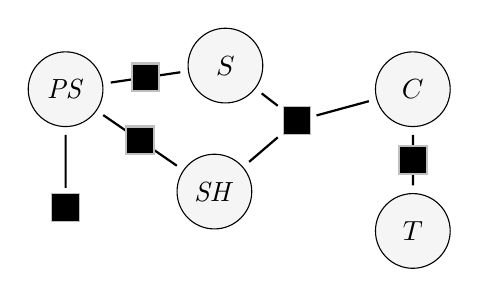
\begin{tikzpicture}[center base, xscale=1.4,
		fgnode/.append style={minimum width=2.7em, inner sep=0.3em}]
		\node[factor] (prior) at (1.65,-1) {};
		\node[factor] (center) at (3.75, 0.1){};
		
		\node[fgnode] (PS) at (1.65,0.5) {$\mathit{PS}$};
		\node[fgnode] (S) at (3.1, 0.8) {$S$};
		\node[fgnode] (SH) at (3.0, -0.8) {$\mathit{SH}$};
		\node[fgnode] (C) at (4.8,0.5) {$C$};
		
		\draw[thick] (prior) -- (PS);
		\draw[thick] (PS) --node[factor](pss){} (S);
		\draw[thick] (PS) --node[factor](pssh){} (SH);
		\draw[thick] (S) -- (center) (center) -- (SH) (C) -- (center);

%		\node[dpadded, fill=blue] (1) at (2.5,-2) {1};
%					
%		\draw[blue!50, arr] (1) -- (prior);
%		\draw[blue!50, arr] (1) -- (center);
%		\draw[blue!50, arr] (1) -- (pss);
%		\draw[blue!50, arr] (1) -- (pssh);
		
		%oli24:
		% \node[fgnode, fill opacity=0.02,dashed] (T) at (4.8, -1.3) {$T$};
		\node[fgnode] (T) at (4.8, -1.3) {$T$};
		\draw[thick] (T) -- node[factor]{}  (C);	
		% \node[factor, draw=black, pattern=north east hatch] at (Q){};
	\end{tikzpicture}
	\fi
	%oli22:improving spacing.
        % ~\vrule~
	\hfill\vrule\hfill
		% \end{subfigure}
		% \begin{subfigure}{0.5\linewidth}\centering
	\ifprecompiledfigs
\raisebox{-0.5\height}{\includegraphics{figure-pdfs/smoking-convert}}
% \raisebox{-0.5\height}{\includegraphics{smoking-convert}}
	\else
	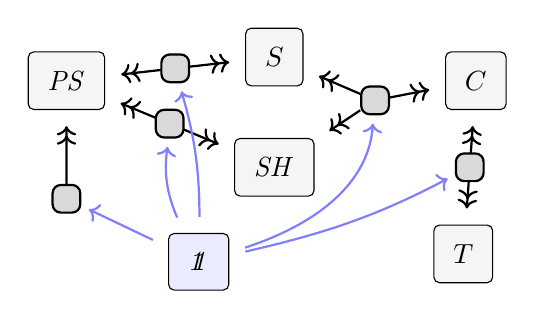
\begin{tikzpicture}[center base, xscale=1.6,
        newnode/.style={rectangle, inner sep=5pt, fill=gray!30, rounded corners=3, thick,draw}]
		\node[newnode] (prior) at (1.65,-1) {};
		\node[newnode] (center) at (4.1, 0.25){};
		
		\node[dpadded] (PS) at (1.65,0.5) {$\mathit{PS}$};
		\node[dpadded] (S) at (3.3, 0.8) {$S$};
		\node[dpadded] (SH) at (3.3, -0.6) {$\mathit{SH}$};
		\node[dpadded] (C) at (4.9,0.5) {$C$};
		
		\draw[arr, ->>, shorten <=0pt] (prior) -- (PS);
		\draw[arr, <<->>] (PS) --node[newnode](pss){} (S);
		\draw[arr, <<->>] (PS) --node[newnode](pssh){} (SH);
		\draw[arr, <<-, shorten >=0pt] (S) -- (center); 
		\draw[arr, <<-, shorten >=0pt] (SH)-- (center); 
		\draw[arr, <<-, shorten >=0pt] (C) -- (center);
		
		%oli29: missed one \var 1
		% \node[dpadded, fill=blue] (1) at (2.7,-1.8) {1};
		\node[dpadded, fill=blue] (1) at (2.7,-1.8) {$\pdgunit$};
		
		\draw[blue!50, arr] (1) -- (prior);
		\draw[blue!50, arr] (1) to[bend right=30] (center);
		\draw[blue!50, arr] (1) to[bend right = 5] (pss);
		\draw[blue!50, arr] (1) to[bend left = 10] (pssh);

		
		\node[dpadded] (T) at (4.8, -1.7) {$T$};
		\draw[arr, <<->>] (T) -- node[newnode](tc){}  (C);	

		\draw[blue!50, arr] (1) to[bend right = 10] (tc);
	\end{tikzpicture}
	\fi
		% \end{subfigure}
	\hfill~
	\caption{
%oli20: oops garbled. Fixing.
% The conversion from a PDG to a factor graph to factor
% graph, and vice versa, as defined in \Cref{def:fg2PDG}. The
%joe18: still garbled
%Conversion of the PDG in \cref{ex:smoking} a PDG to a factor graph
Conversion of the PDG in \cref{ex:smoking} to a factor graph
according to \cref{def:PDG2fg} (left), and from that factor graph back
to a PDG by \cref{def:fg2PDG} (right). 
%joe17
%blue edges carry the (renormalized) cpds corresponding to the
%joe18: what does ``renormalized'' mean here?  Why did the cpds have
%to be renoormalized
%oli21: because they're now being regarded as unconditional distributions. To
%illustrate: both a cpt X -> Y and an unconditional distribution 1 -> XY are
%matrices. In the first case, each row sums to 1, whereas in the second, the
%whole matrix sums to 1. We're renormalizing the cpd so that they are
%unconditional distributions. I think your original edit introduced
%this ambiguity.
%joe19*: I'm lost.  Why are they now being regarded as unconditional
%distributions?  I'm OK with the current caption.
%oli21: let me try again to write this clearly.
	% In the latter, blue edges are associated with the cpds corresponding to the
	% original factors, each leading to a new node $X_J$ (displayed as a
	% smaller darker rectangle) whose values are joint settings of the
	% variables connected to the factor $J$. 
%
%joe19
%In the latter, for each $J$ we intorduce a new node $X_J$ (displayed as a
%smaller darker rectangle) whose values are joint settings of the
In the latter, for each $J$ we introduce a new variable $X_J$ (displayed as a
smaller darker rectangle), whose values are joint settings of the
variables connected it, and also an edge $1 \to X_J$ 
%joe19
%(blue)
(shown in blue),
%oli21: AAAI only begrudgingly accepts color I will make sure all the 
% figures, etc. look good in black and white later.
%FIXME
%joe19
%to which we associate with the unconditional
to which we associate the unconditional 
distribution given by normalizing $\phi_J$.
} 
	\label{fig:fg2PDG}
\end{figure*}


%joe1: rewrote
%Surprisingly, despite garbling the structure (see
%\Cref{fig:fg2PDG,fig:fg-intro-examples}), when we fix $\gamma=1$, the
%two operations preserve most of their semantics.
PDGs are directed graphs, while factors graphs are undirected. The
map from PDGs to factor graphs thus loses some important structure.
As shown in
%joe17: I get problems when I latex this.  It says ``As shown in
%Figures 8 and 9 in Figure 9''. Moreover, the actual figure is Figure 4.
%oli20: another problem with comments... should be fixed now. 
\vfull{
    \Cref{fig:fg2PDG,fig:fg-intro-examples}
}%\end{vfull}
\Cref{fig:fg2PDG},
%joe11
%the mappings can change the graphical structure signfiicantly.
%oli24: actually it's just the second one.
% the mappings can change the graphical structure significantly.
this mapping can change the graphical structure significantly.
%oli12: no \alphas, so we have something slightly different is true.
% Nevertheless, if we take $\gamma=1$,
%oli22: As you say in a %joe18* below, let's just state the theorems,
% and then describe useful corolaries, instead of building up to them with
% the theorem statements below, which are evidently quite confusing. 
	% Nevertheless, in the case where every weight is the same,
Nevertheless,
%oli23: not quite true; removing together with the theorem below.
% if we start with an unweighted factor graph, then
% applying the two conversions take us back to the same factor graph, so
% each is the inverse of the other.  Moreover, 
%oli23: we can substantially strengthen this claim now.
% in the case where all the
% weights are the same, then
%oli24: added emphasis & cqualifier
% both conversions preserve the semantics.
%joe22
%\emph{both} conversions preserve the $\gamma=1$ semantics.
%oli25: this is related to the only other major comment in this round of
% edits, so I'll defer discussion until then, but briefly: I think by saying
% 'in the special case' you give the result is mroe restricted than it is;
% this feels off to me for the same reason that 
% "you can see the red color of a cherry in the special case in which you are
% looking at it" seems wrong. A PDG has semantics for ALL gammma, and this is
% a particular one. Rewording differently.
% both conversions preserve the semantics in the special case that $\gamma=1$. 
%joe23: Well, I think it is a special case, but Im OK with your
%wording.  Just correcting a typo; you should probably do a spellcheck
%both conversions preserve the semantics correpsponding to $\gamma=1$.
%joe25
%both conversions preserve the semantics corresponding to $\gamma=1$.
%oli27: I used "corresponding to" instead of "when" because to me
%"when" makes it 
% sound like \gamma is handed to you, but we get to set \gamma. 
% It's an indexed family of semantics, for every gamma, and we have some choice
% at which one we're looking at. How is "at"? Or "for"? 
% both conversions preserve the semantics when $\gamma=1$.
%joe26: undid; ``semantics at \gamma = 1'' is meaningless (as is
%``semantics corresponding to \gamma=1''.  There is no semantics
%``at'' or ``corresponding to'' gamma=1.  We preserve the semantics
%when \gamma=1, and not when \gamma has some different value.  I could
%live with ``for'', although ``when'' is definitely better English
%both conversions preserve the semantics at $\gamma=1$
%oli27: Moving the recollection of unweighted PDGs here.
% Original is below; I have modified it also, because I think "identify" is too strong.
% (recall that we identify the unweighted PDG $(\Gr,\mat p)$ with the
% weighted PDG $(\Gr,\mat p,  \mat 1, \mat 1)$).
%joe26: No!  If you put it here, you'll confuse the reader?  ``Why are
%you reminding me of this now?''  Put it where you use it -- that is,
%at the point where the reader is likely to be confused.  I could live
%with making it a footnote, but this is the wrong place for it.  

% Also, changing the "the" to an "an".
%joe21
% both conversions preserve the semantics, if we associate the
% unweighted PDG $\dg N$ with the (weighted) PDG $(\dg N,{\bf 1})$
% (i.e., we take $\beta$ to be the constant function {\bf 1}).
%oli24: I find this comes off as way less ad-hoc if we don't
% make this definition last-minute. I'm introducing this convention at the
% beginning, along with our convention about \alpha.

%oli22: commenting out the less general theorems.
%joe20*: reinstasting, as we agreed
%oli9: this holds more generally, illustrating that PDGs can carry factor graph data regardless of \theta, \beta.
%oli23: removing because to make it correct we either need to 
% weaken it by taking the probabilities, as was done in the version
% that the %oli9 comment above was arguing for, or state
% that it holds up to the equivalence of removing the extra coherence
% structure we've introduced --- it is merely that the collection of factors
% is the same.
\commentout{
	\begthm{prop}{prop:fg-pdg-lossless}
	%joe20*:
	%$\Phi \circ \PDGof = \mathrm{Id}_{\text{FG}}$. That
	%		is, if $F$ is a factor graph, then
	%		$\Pr_{\Phi(\PDGof{F})} = \Pr_F$.
	Given an unweighted FG $\Phi$, $\Phi_{\UPDGof{\Phi}} = \Phi$ 
	\end{prop}
}

%oli23*: Preserving this discussion, rewriting the unweighted versions from scratch
\commentout{
	% \begthm{theorem}[restate=thmpdgisfg]\label{thm:pdg-is-fg}
	\begthm{theorem}{thm:pdg-is-fg}
	%oli20: ok let's be more careful. What is 'gamma'?
	% If $\dg M$ is a PDG with $\beta_L = \gamma$ for all 
	%joe18: I actually thought it was fine before, but I'm OK with the
	%following slight reweroding
	%If $\dg M$ is a PDG, and $\gamma$ is a number such that $\beta_L\!
		If $\dg M$ is a PDG such that for some $\gamma >0$, we have that $\beta_L\!
		= \gamma$ for all  $L$, then
	%oli21: your reword (above) has the structure:
	% if [exists \gamma ... ] then  [\phrase involving \gamma], which 
	% muddles quantifiers, but I don't like my fix (below) so I'll leave yours.
		% If $\dg M$ is a PDG and $\gamma > 0$ satisfies $\beta_L\!
		% = \gamma$ for all  $L$, then
	$\bbr{\dg M}_{\gamma} = \gamma\,\GFE_{ \WFGof{\dg M} }$ and
	$\bbr{\dg M}_{\gamma}^* = \{\Pr_{ \WFGof{\dg M}} \}$.
	%oli21: to do it directly in the old notation (I find it 
	%cluttered and difficult to parse, which is why I changed it)
	% $\bbr{\dg M}_{\gamma} = \gamma\,\GFE_{ \WFGof{\dg M}, \beta^{\dg M}}$ and
	% $\bbr{\dg M}_{\gamma}^* = \{\Pr_{ \Phi_{{\dg M}},  \beta^{\dg M}} \}$.
	\end{theorem}
	\begthm{theorem}{thm:fg-is-pdg}
	%joe19*: You should work with WFGs everywhere, and use \Psi
	Given a factor graph $\Phi$, 
	and a constant vector $\kappa = \{ k \}_{J \in \cal J}$ for some fixed $k$, then
	we have that
	$\GFE_{\Phi, \kappa} = \nicefrac{1}{k}\bbr{\PDGof{\Phi,\kappa}}_{k} + C$  
	for some constant $C$, so $\Pr_{\Phi, \kappa}$ is the unique element of 
	$\bbr{\PDGof{\Phi,\kappa}}_{k}^*$. 
	\end{theorem}
}%oli23: endcommentout

%oli23*: here are the unweighted analogs.
\begthm{theorem}{thm:fg-is-pdg}
%oli24: I placed the comment in the beginning; this is really not as ad-hoc
% as this notation makes it seem.
%joe22* You have to remind the reader of this convention!  It's not OK
%to use it pages after you've defined 3 pages back (which the reader
%probably missed) it without a reminder.  Be nice to the reader!
%joe23*: I'm willing to live with your notation, but you *must* remind
%the rader of it.  (I would actulaly put the definition here, rather
%than 3 pages back, since I don't belive you use it except for here.
%This is an instance of a general principal: define a notion when you
%need it.  I see no class of reader for which there's a benefit it in
%defining it on page 3 and using it for the first time on p. 6.
%oli25*: I believe that which choice is better depends on what kind of
%reader.  There are at least two classes of reader for which I think
%my version is substantially better: (1) those who are skimming and
%not tracing definitions carefully (because 
% it's simpler and less confusing than the version with the 1, which requires
% a little more notation tracing about what the 1 is (is it \alpha?\beta? What 
% does that do exactly again?), (2) those who are familiar with factor
% graphs and  
% instintcively take unweighted = weights all 1.
%joe25*: I'm sure that there are some readers out there somewhere for
%whom it is good to define something 3 (double-column) pages before
%it's used, but this is not the case for the great majority of
%readers.  We shouldn't do it.  
% I believe also that there are readers who would appreciate the ${\bf 1}$, but
% I also have a strong aethetic preference to leaving it out. I think putting the
% \bf 1 inside makes it look more complicated than it is, and that it depends on
% more parameters than it does. The detail is technically correct and admittedly
% makes it a more careful presentation in some ways, but you have vehemently 
% objected to other ways in which I have wanted to do things more carefully
% (e.g., adding my type annotations to definitions).  Again, I think making
% a big deal of this is putting emphasis in the wrong place.
$\Pr_{\Phi} = \bbr{\UPDGof{\Phi}}_{1}^*\;$ for all factor graphs
%joe25*: added: please do not bother discussing it.
%oli27*: I accept this change, but my sense of aesthetics demands that it be 
% moved outside of the Theorem for symmetry. It is slightly reworded above.
%joe26: I'm afraid helping the reader trumps your aesthetic sense.
%You can make it a footnote if that helps, but please don't move it
%somewhere unhelpful.  I can live with ``treat'' (although, for the
%life of me, I can't see why that's better).
%oli29:Regarding why I prefer to
%	avoid "identify":  (N, \alpha, \beta) is a PDG, but ((N,1,1) \alpha,\beta)
%	has too many weights. It is conceptually important that there is a distinction
% 	between a weighted and unweighted PDG, even though the semantics treat them the
%	same way.
%oli29: I feel compelled to put it in the footnote. Also, to use "treat",
%	some additional words must be changed also; somehow this got dropped
%	in the last document I sent you. In the commented out version, I'm leaving
%	"identify".
% $\Phi$ (recall that we identify the unweighted PDG $(\Gr,\mat p)$ with the
%  weighted PDG $(\Gr,\mat p,  \mat 1, \mat 1)$).
%joe28: I can live with it in a footnote, and could have lived with
%``treat'', but ``semantically like'' is meaningless.  Reverting back.
%$\Phi$.\footnote{recall that we treat the unweighted PDG $(\Gr,\mat
%p)$ semantically like the weighted PDG $(\Gr,\mat p,  \mat 1, \mat 1)$.}  
$\Phi$.\footnote{Recall that we identify the unweighted PDG $(\Gr,\mat
p)$ with the weighted PDG $(\Gr,\mat p,  \mat 1, \mat 1)$.}  
%joe21
% $\Pr_{\Phi} = \bbr{(\UPDGof{\Phi},{\bf 1})}_{1}^*\;$ for all factor graphs $\Phi$.
\end{theorem}
\begthm{theorem}{thm:pdg-is-fg}
%oli24: and again
$\bbr{\dg N}_{1}^* = \Pr_{\FGof{\dg N}}\;$ for all unweighted
%joe21*
% $\bbr{(\dg N, {\bf 1})}_{1}^* = \Pr_{\FGof{\dg N}}\;$ for all unweighted
	PDGs $\dg N$.  
\end{theorem}
%oli23*: added important discussion.
The correspondence hinges on the fact that we take $\gamma=1$, so that $\Inc$ and
$\IDef{}$ are weighted equally.
%oli24: important discussion.
%joe22*: I find this discussion problematic, since we haven't
%discussed where teh choice of \gamma is coming from. It's not at all clear
%to me that this limitation is unproblematic.  We've solved a problem
%by giving the modeler the freedom to choose k without explaining why
%a particular choice is OK.  I think that the paper is worse off by
%this addition; you're just reminding the reader of our unmotivated
%choices (which I viewed as technical means to get a result, rather
%than natural modeling choices).  
%oli25*: You may view it as a technical means to get the paper to work out,
% but I definitely do not view it that way.
%joe25: you're of course entitled to view it any way you like, but we
%don't have the time or space to get into it here.
%joe23*: I understand that, but we don't exlain your point of view in
%the paper.   We have given no basis on which to claim something is ``not
%problematic''.   Saying it is will raise flags, so is a net negative.
%Similarly for the claim that we can't get a factor graph to
%``replace'' a PDG.  If a user is perfectly happy with a
%representation using a factor graph, why should he/she want to
%replace it by a PDG?  There is perhaps a point to be made here, but
%it needs to be written in a way that seems reasonable to a reader who
%hasn't read your mind and does not necessarily agree with our viewpoint.
%Moreover, the way the
% paper is currently 
% written, I think that \gamma is motivated fairly well (it's a
% trade-off between 
% a quantiative (by which I mean, "dependent on the cpds") and qualitative (by 
% which I mean, "dependent only on the graph structure") term, and readers
% with some imagination will have some ideas for how to use this. I
% certainly do. 
% In any case, here we only say that it indexes the family of a semantics, whch
% is just another technical fact, and I thiknk drawing attention to it strengthens
% our point a lot.
Because the user of a PDG gets to choose $\gamma$, the fact that the 
%joe25: the \gamma = k is a typo, I assume.  I don't know what it
%means for a translation to ``hold''
%translation from WFGs to PDGs holds only for $\gamma=k$ is not problematic;
%oli27: oops: Haven't defind a "WFG" yet.
% translation from WFGs to PDGs preserves semantics only for $\gamma=1$
%joe26: I left in the ``for'', although, as I said above, ``when''
%would be better English
translation from factor graphs to PDGs preserves semantics only for $\gamma=1$
%oli27: clarifying what the lack of "problem" is.
% is not problematic;. 
% makes it easy to emulate a factor graph with PDG semantics. 
%joe26: PDGs are not agents.  They don't try to do anything
%poses no problem for a PDG trying to emulate a factor graph.  It's
%the user that has or doesn't have a problem.
poses no problem.
%joe25: I don't know what it means to set \gamma so as to vie the
%original factor graph  I cut this.
%the user can simply set $\gamma$ so as to view the original factor graph.
%joe25: This seemed much too fuzzy to me
%However, in translating back, we lose this ability, making it very
%difficult for a factor graph replace a PDG.
%oli27: Agreed. Some further edits:
% However, the fact that the translation in the other direction
% preserves semantics only if $\gamma=1$ suggest that factor graphs are
% less flexible than PDGs.
Conversely, the fact that the reverse correspondence requires
$\gamma=1$ suggests 
that factor graphs are less flexible than PDGs.

%joe21
%What about weighted PDGs, of the form $(\Gr, \mat p, \beta)$?
%Factor graphs, too, have a standard notion of weightedness, 
%but so long as we stick with our convention of setting every $\alpha_L = 1$, 
%we cannot say much about them.
What about weighted PDGs $(\Gr, \mat p, \beta)$ where $\beta \ne {\bf 1}$?
There is also a standard notion of weighted factor graph,
but as long as we stick with our convention of taking  $\alpha = {\bf 1}$, 
we cannot relate them to weighted PDGs.  
%oli24: squeezing some more space
% As we show in the next section,
As we are about to see,
once we drop this convention, we can do much more.

%joe18*: rewrote.  Assuming we keep this, the real question is where
%we introduce \alpha.  If we introduce it at the beginning, then we
%need to include it in the BN theorem and were really should give more
%intuition (which we'll have a hard time agreeing on, based on past
%history), although perhaps we can get away with saying that we'll
%just use it in a technical way.  Obviously, if we include it, we
%shold get rid of Theorems 4.2 and 4.3, and just use the stronger version. 
%oli22:  agree with the sentiment above,
% but was not able to reorganize enough of the document to make that happen 
% last time. I'm attempting it this time, which is why the present section
% is commented out.
%These theorems above are actually quite restrictive:
%	both \cref{thm:pdg-is-fg,thm:fg-is-pdg} require that the
%	confidences be uniform,  
	% and even then only offer a correspondence for a specific value of $\gamma$, which makes it impossible to even consider our limit.
%oli23*:
% This is not the right story. The theorems are restrictive
% because PDGs are not
\commentout{
	These theorems are quite restrictive:  Theorem~\ref{thm:pdg-is-fg}
	applies only to PDGs where all the uncertainties $\beta_L$ are
	identical, while Theorem~\ref{thm:fg-is-pdg} applies only to factor
	graphs where all weights $\Theta_J$ are identical.  We can generalize
	%joe19*: 
	%Theorem~\ref{thm:pdg-is-fg} slightly to the case where the ratio of
	Theorem~\ref{thm:pdg-is-fg} slightly by allowing $\alpha_L$ to have
%joe21
%values other than 1.
values other than ${\bf 1}$.
	%joe20*: added, since you never said this
	That is, we now consider PDGs of the form $(\Gr,\mat
	p, \alpha,\beta)$, where $\alpha_L$ can have arbitrary non-negative values.
	We generalize the translation given in Definition~\ref{def:fg2PDG} by
	allowing a family of translations, parameterized by $\gamma$.
	Specifically, given a WFG $\Psi$, we take $\PDGof{\Psi,\gamma} =
	(\UPDGof{\Phi},\beta_{\theta}/\gamma, \beta_{\theta})$. 
}


\subsection{Factored Exponential Families}\label{sec:expfam}
%oli23* insertion




%li23: acronym? did not make change.
% We take a \emph{weighted factor graph}  $\Psi$ to be a pair
%joe21
%We take a \emph{weighted factor graph} $\Psi$ to be a pair
A \emph{weighted factor graph (WFG)} $\Psi$ is a pair
$(\Phi,\theta)$ consisting of a factor graph $\Phi$ 
together with a vector of non-negative weights
$\{ \theta_J \}_{J \in \mathcal J}$.
$\Psi$ specifies a canonical scoring function 
\begin{equation}
\GFE_{\Psi}(\mu)
%   \GFE_{(\Phi,\theta)}(\mu)
	 := \!\Ex_{\vec x\sim\mu}\left[  \sum_{J \in
           \cal J} \theta_J \log\frac1{\phi_J(\vec
               x_J)}\right] - \H(\mu)  , 
			   \label{eqn:free-energy}
\end{equation}
%joe20
%which $\Pr_{(\Phi,\theta)}$ minimizes, called the \emph{variational
%oli23:
% which $\Pr_{\Psi}$ minimizes,
called the \emph{variational
Gibbs free energy} \cite{mezard2009information}. 
%oli23:
$\GFE_{\Psi}$ is uniquely minimized by the distribution
${\Pr}_{\Psi}(\vec x) = \frac{1}{Z_{\Psi}}
%oli26: [reviewer #7] fix equation 
 	% \prod_{J \in \cal J} \phi_J(\vec x_J)$, 
 	\prod_{J \in \cal J} \phi_J(\vec x_J)^{\theta_J}$, 
which matches the unweighted case when every $\theta_J = 1$.
The mapping $\theta \mapsto \Pr_{(\Phi,\theta)}$ is known as 
%joe20
%$\Phi$'s exponential family and is a central tool in the analysis
$\Phi$'s \emph{exponential family} and is a central tool in the analysis  
and development of many algorithms for graphical models \cite{wainwright2008graphical}.

PDGs can in fact capture the full exponential family of a factor graph, but only
%oli24
by allowing values of $\alpha$ other than ${\bf 1}$. In this case, the
only definition  
% by allowing values of $\alpha$ other than 1. In this case, the only definition 
that requires alteration is $\IDef{}$, which now depends on the \emph{weighted multigraph}
$(\Gr^{\dg M}, \alpha^{\dg M})$, and is given by
\begin{equation}
%oli24: Let's just define it for M;
	% \IDef{G}(\mu) := \sum_{\ed LXY \in \Ed} \alpha_L \H_\mu(Y\mid X) - \H(\mu). 
	\IDef{\dg M}(\mu) := \sum_{\ed LXY \in \Ed} \alpha_L \H_\mu(Y\mid X) - \H(\mu). 
	\label{eqn:alt-extra2}
\end{equation}
%joe21: rewrote.  The reader won't know what (b) is
%In ths case, each specification in~\ref{item:localinfo} may be
%weighted by differently, so that some edges are more qualitatively
%certain than others, and correspondingly it may be more or less
%important to describe them properly.
Thus, the conditional entropy $\H_\mu(Y\mid X)$ associated with the
edge $\ed LXY$ is multiplied by the weight $\alpha_L$ of that edge.

%oli23: taken from your text.
%oli24: Softening slightly
% The key benefit of using $\alpha$ is that we can
One key benefit of using $\alpha$ is that we can
capture arbitrary WFGs, not just ones with a constant weight
vector.    All we have to do is to ensure that in our translation from
factor graphs to PDGs, the ratio $\alpha_L/\beta_L$ is a
constant.  (Of course, if we allow arbitrary weights, we cannot hope
to do this if $\alpha_L = 1$ for all edges $L$.)  
%oli23: new
%joe21
%We therefore define a family of translations.
We therefore define a family of translations, parameterized by the
ratio of $\alpha_L$ to $\beta_L$.
\begin{defn}[WFG to PDG]\label{def:wfg2pdg}
Given a WFG
%joe20*: going back to the special case of \alpha=1, AS WE HAD AGREED.   What
%do we do for edges not in \J.   I also don't think that this is quite
%right, sonce you haven't defined \beta for edges not in \J.  I now do
%so, although you should check 
%$\Psi=(\Phi, \theta)$ to a PDG $\PDGof{\Psi} = (\UPDGof{\Phi},\theta, \theta)$ 
$\Psi=(\Phi, \theta)$,
and postive number $k$, 
we define the corresponding PDG $\PDGof{\Psi,k} = (\UPDGof{\Phi},\alpha_{\theta}, \beta_{\theta})$ 
%by taking both $\alpha$ and $\beta$ to be $\theta$.
by taking $\beta_J = k \theta_J$ and $\alpha_J = \theta_J$ for the edge
%oli29: missed another one
 % $1  \rightarrow X_J$, and
 $\pdgunit  \rightarrow X_J$, and
%oli24:
taking $\beta_L = k$ and $\alpha_L = 1$ for the projections $X_J \!\tto\! X_j$.
% taking $\alpha_L = 1$, $\beta_L = k$ for the projections $X_J \!\tto\! X_j$.
\end{defn}

%joe21*: Cut  I don't like the notion of capturing data.  More
%importantlly,
%We now turn to extend \cref{def:PDG2fg}.  
%Since PDGs have two sets of weights, and WFGs only have one,
%we will not be able to capture all the data.
We now extend Definitions~\ref{def:PDG2fg} and \ref{def:fg2PDG} to
(weighted) PDGs and WFGs.  
%oli24:
%In going translating from PDGs to WFGs, 
In translating a PDG to a WFG, 
%oli24: the mismatch isn't just a problem for this direction
% note that we have somewhat of a mismatch: PDGs have two sets of weights, and WFGs
there will necessarily be some loss of information: PDGs have two sets, while WFGs have 
%oli24:
% only have one, So in our translation, we ingore $\alpha$, and consider
only have one. Here we throw out $\alpha$ and keep $\beta$, 
%oli24: added
%joe22*: I have no clue what this addition means.  I also think it's a
%mistake to highlight another ad hoc choice.  I strongly prefer my wording.
%oli25*: I find it very strange what ad-hoc choices you want to hide
% and which ones you want to expose.
%joe23*: we can debate which ad hoc choices to hide (my own feeling
%is: as many as possible).   What is not open
%to debate is the fact that I didn't understand what you wrote.  To
%the extent that I'm somewhat representative (whch I believe I am),
%this must be rewritten.  
%There are many places where I
% feel there is  
% genuinely something there, and when you don't understand my descriptions, we 
% settle on a description of it which (in my view) far undersells our 
% contribution. Here, this is truly an ad-hoc choice, and I have no problem 
% admitting it (we're claiming there's not even a good choice to be had), 
% and it seems you're trying to just state some facts so it seems our particular
% choice is better than some other choices. It's just a choice, and I think 
% that letting the reader know is useful.
though in its role here as a left inverse of \cref{def:wfg2pdg},
%oli27: minor word tweak
% chosing either would suffice
either choice would suffice. 

%there are more PDGs than WFGs, and so there is not a perfect way to
%translate back. 
%We have chosen here to preserve $\beta$.

\begin{defn}[PDG to WFG]
Given a (weighted) PDG $\dg M =
(\dg N, \beta)$, we take its corresponding WFG to be $\WFGof{\dg M} :=
%joe21
%(\FGof{\dg N}, \beta)$ by setting $\theta_L := \beta_L$.
(\FGof{\dg N}, \beta)$; that is, $\theta_L := \beta_L$ for all edges $L$.
\end{defn}



%joe19*: 
%oli22: blank %joe19*.

%oli22: I'm actually also cutting the current presentation of these theorems
% and re-stating them below, 
% using un-weighted objects + weights, which I think is far less confusing.
% allows the most general theorems to be put right away without special
% conversions and specific discussion about what to do with \alpha.
\commentout{
\begthm{theorem}{thm:pdg-is-fg2}
%joe18
%If $\dg M$ is a PDG, and $\gamma$ is a number such that
If $\dg M$ is a PDG such that for some $\gamma >0$, we have that
	$\beta_L = \alpha_L \gamma$ for all  
	%oli12 line shave
	%edges
	$L$, then
	$\bbr{\dg M}_{\gamma} = \gamma\,\GFE_{\Phi_{\dg M}} $ and
	$\bbr{\dg M}_{\gamma}^* = \{\Pr_{\Phi_{\dg M}} \}$.
	 	% $\kldiv{\mu}{\Pr_{\Phi(\dg M)}} = \bbr{\dg M}_{1}(\mu)$
		% In particular, $\Pr_{\Phi(\dg M)} = \bbr{\dg M}_*^{\gamma := 1}$
\end{theorem}

%joe19

% \begin{theorem}[restate=thmfgispdg]\label{thm:fg-is-pdg}

%joe18* unless I'm missing something, you need to redo Definition 4.3
%to explain how to add the \alphas.  Will you add them in such a way
%that the ratio of \beta_L to \alpha_L is constant?  If so, we can say
%that because the construction made it a constant, the following result holds.
%If the updated Definition 4.3 allows some flexibility in
%choosing \alpha and \beta, then this would reqire more work.
%oli21: Oops, I forgot to add those two characters; we set \alpha_L = \beta_L. 
% In any case, I think the true things you say above can be sold better:
%joe19: As I said, I don't believe that you want \alpha_L = \beta_L
%oli22**: Since in general we cannot know gamma (because the translation meerely
% supplies the data of the PDG, including alpha and beta, but a user can
% laterquery the semantics for multiple different values of gamma),
% we can't do any better than to set them to be proportional. 1 is a nice
% nice multiplicative constant generally, and also is speial because that's the 
% one we need to capture unweighted factor graphs with unweighted PDGs.

%joe19*: AARGH!  I was hoping that you would discuss the more general
%translation here, where \alpha could be arbitrar.  I don't believe
%that the reslt will hold if \alpha_L = \beta_L.  As you ptoint out,
%we need \beta_L = \alpha_L \gamma not \alpha_L = \beta_L.  So
%although you spent a lot of time doing what I explicitly asked you to
%do, you didn't address my main concerns.  You absolutely did not
%explain how to do  the translation when you have an abtrary weight vector.
%specify how you do the translatin here from factor graphs to PDGs.
%I put in what I think you should have put in.
%oli22: As stated in emails, I believe your conversion is correct but 
% slightly deceptive. I have therefore recycled 
The key benefit in using $\alpha$ is that we can
capture arbitrary WFGs, not just ones with a constant weight
vector.    All we have to do is to ensure that in our translation from
factor graphs to PDGs, the ratio ratio $\alpha_L/\beta_L$ is a
constant.  (Of course, if we allow arbitrary weights, we cannot hope
to do this if $\alpha_L = 1$ for all edges $L$.)

Specifically, given
$0 < \gamma \le 1$ and a WFG $\Psi = (\Phi,\theta)$, we take the PDG
${\dg M}_{\Psi,\gamma}$ to be defined just like the PDG ${\dg M}_\Psi$ of
Definition~\ref{def:fg2PDG}, except that instead of having $\alpha_L =
1$, we have $\alpha_L = \gamma\beta_L$. 


	\begthm{theorem}{thm:fg-is-pdg2}
	%oli20: we got to remove the condition!
%joe19
%For every factor graph $\Phi$, and EVERY vector $\theta$ over $\cal J$
For all WFGs $\Psi = (\Phi,\theta)$ and all $\gamma$ with $0
< \gamma \le 1$
	%, and EVERY $\gamma >0$
	we have that
	% for any joint distribution $\mu$ on $\V(\mathcal X)$, we
	        % have $\kldiv{\mu}{\Pr_\Phi} = \bbr{\PDGof{(\Phi)}}_{1}(\mu)$ 
	%joe8: again
	%oli10: adding back in
	%joe9
	        %	$\gamma \GFE_\Phi = \bbr{\PDGof{(\Phi)}}_{\gamma} + k$
	        %        where $k$ is a constant, and in particular, 
%joe19*
%$\GFE_\Phi = \nicefrac1{\gamma} \bbr{\PDGof{\Phi,\theta}}_{\gamma} + C$  
$\GFE_\Psi = \nicefrac1{\gamma} \bbr{\PDGof{\Psi,\gamma}}_{\gamma} + C$  
for some constant $C$, so
%joe19*
%$\Pr_{\Phi, \theta}$ is the unique element of
%$\bbr{\PDGof{\Phi,\theta}}_{\gamma}^*$.
$\Pr_{\Psi}$ is the unique element of
$\bbr{\PDGof{\Psi,\gamma}}_{\gamma}^*$.  
	   % Moreover, $\Pr_{\Phi, \theta} = \bbr{\PDGof{\Phi,\theta}}^*$.
	\end{theorem}
}%oli22: \end{commentout}

%oli22**: big insertion: both of the above theorems + recycled material
% from your discussion. 
%joe20: note that I changed the label
%\begthm{theorem}{thm:pdg-is-fg}We can can now generalize our earlier results 


%oli23: canabalized for the above.
% %joe20*: resinstated
% The key benefit of using $\alpha$ is that we can
% capture arbitrary WFGs, not just ones with a constant weight
% vector.    All we have to do is to ensure that in our translation from
% factor graphs to PDGs, the ratio $\alpha_L/\beta_L$ is a
% constant.  (Of course, if we allow arbitrary weights, we cannot hope
% to do this if $\alpha_L = 1$ for all edges $L$.)  Specifically, given
% $0 < \gamma \le 1$ and a WFG $\Psi = (\Phi,\theta)$, we take the PDG
% ${\dg M}_{\Psi,\gamma}$ to be defined just like the PDG ${\dg M}_\Psi$ of
% Definition~\ref{def:fg2PDG}, except that instead of having $\alpha_L =
% %joe20
% %1$, we have $\alpha_L = \gamma\beta_L$.
% 1$, we have $\alpha_L = \beta_L/\gamma$. 

%oli24: double now. Also this gives me a line.
% We now show that we can now capture the entire exponential family of a factor graph,
We now show that we can capture the entire exponential family of a factor graph,
%oli24: let's boast a little about this; we haven't mentioned it yet
and even its associated free energy, 
%joe21
%but only for the value of $\gamma$ equal to the constant $k$ used in
but only for $\gamma$ equal to the constant $k$ used in
the translation.  


\begin{theorem}\label{thm:wfg-is-pdg}
For all WFGs $\Psi = (\Phi,\theta)$ and all $\gamma > 0$,
we have that
$\GFE_\Psi
%joe20*: using notation defined above
%= \nicefrac1{\gamma} \bbr{(\UPDGof{\Phi}, \theta, \nicefrac{1}{\!\gamma\,}\theta)}_{\gamma}
= \nicefrac1{\gamma} \bbr{{\dg M}_{\Psi,\gamma}}_{\gamma} 
+ C$   
for some constant $C$, so
$\Pr_{\Psi}$ is the unique element of
%joe20*: switching alpha and beta again, and using \beta_\theta
%instead of \theta
%$\bbr{(\UPDGof{\Phi}, \theta, \nicefrac{1}{\!\gamma\,}\theta)}_{\gamma}^*$.  
$\bbr{{\dg M}_{\Psi,\gamma}}_{\gamma}^*$.
\end{theorem}

%joe21
%In particular,for $k\!=\!1$, so that $\theta$ is used for both
In particular, for $k\!=\!1$, so that $\theta$ is used for both the functions
$\alpha$ and $\beta$ of the resulting PDG,
\cref{thm:wfg-is-pdg} strictly generalizes \cref{thm:fg-is-pdg}.
\begin{coro}
	For all weighted factor graphs $(\Phi, \theta)$,
	we have that
	$\Pr_{(\Phi,\theta)} = \bbr{(\UPDGof{\Phi}, \theta,\theta)}_1^*$
\end{coro}

%joe21
%Conversely, so long as the ratio of $\alpha_L$ to $\beta_L$ is constant, the
Conversely, as long as the ratio of $\alpha_L$ to $\beta_L$ is constant, the
reverse translation also preserves semantics.
%oli23: insertaion
% Conversely, we can generalize 
% to the case where the ratio of
% $\alpha_L$ to $\beta_L$ is a constant.
%joe20
%}%oli22 \end{commentout}
\begthm{theorem}{thm:pdg-is-wfg}
For all unweighted PDGs $\dg{N}$ and non-negative vectors $\mat v$
over $\Ed^{\dg N}$, and all $\gamma > 0$, we have that 
%joe20*: you're writing \beta,\alpha; switching it to \alpha \beta,
%and making \beta = v, not \alpha = v.  Does the equality still hold?
%oli27*: oops, almost forgot that this doesn't quite work
% $\bbr{(\dg N, \mat v/\gamma, \mat v)}_{\gamma} 
$\bbr{(\dg N, \mat v, \gamma \mat v)}_{\gamma}
%joe26
%= \gamma\,\GFE_{(\Phi_{\dg N}, \mat v)} $ and consequently
= \gamma\,\GFE_{(\Phi_{\dg N}, \mat v)} $; consequently,
%joe20*
%oli27*:
% $\bbr{(\dg N, \mat v/\gamma, \mat v)}_{\gamma}^*
$\bbr{(\dg N,  \mat v,  \gamma\mat v)}_{\gamma}^*
		= \{\Pr_{(\Phi_{\dg N}, \mat v)} \}$. 
\end{theorem}
% With these translations, factor graphs therefore define a particular subclass
% of PDGs in which the weights $\alpha$ and $\beta$ are proportional.

%oli23: removed
% \noindent Note that if $\beta_L = \gamma$ for all edges $L$, then
% 		$\alpha$ is the 
% constant function 1 in Theorem~\ref{thm:pdg-is-fg1}, so
% Theorem~\ref{thm:pdg-is-fg1} is a generalization of
% Theorem~\ref{thm:pdg-is-fg}. 
%oli23: nevermind 
% We interpret the fact that the correspondence only holds when the constant
% $k$ used in the translation equals $\gamma$, as a reflection of the fact
% that there is no way to articulate a 

%oli22: I've rephrased the statement of the theorem in a suggestive 
% (but kind of clunky) way below.
%I think this is kind of cool, and a neat story. Do you buy it?
%joe20: It's not so much that I don't buy it, but that I can't make
%sense of it.  Where did the product of cpts come from?  Surely you
%must have a factor graf in the picture here.  If you can explain it
%to me in a way that I can understand it, we may want to reinstate
%this. 
%misleading 
%Thus, PDGs in which the quantitative and qualitative certainties are
%fused, when evaluated in the semantics corresponding to the particular
%trade-off coresponding to their cofficient of proportionality,
%precisely generate the exponential family of the associated factor
%graph.
%In particular, our semantics regard an unweighted PDG as a product of
%its cpts, when $\gamma = 1$.
%\begin{coro}\label{coro:justafg} 
%% For all $\dg N \!=\! (\Gr,\mat p)$,
%% If $\dg M$ is an unweighted PDG, then 
%	$\displaystyle\bbr{(\Gr, \mat p)}_1^* 
%		= \frac{1}{Z_{\dg M}}\prod_{\ed LXY \in \Ed^{\dg M}} \bp^{\dg M}(Y \mid X)
%	\propto \!\!\prod_{\ed LXY \mathrlap{\in \Ed^{\dg M}}} \bp(Y \mid X)$.
%\end{coro}
%joe20
\commentout{
We have seen that only a subset of PDGs can be faithfully 
represented as WFGs; we now show the other side of the correspondence: any
factor graph be captured by more than one PDG (though again, only for a fixed $\gamma$).
}

%\begthm{theorem}{thm:fg-is-pdg}





%oli22: end big insertion.

%joe18: cut from here.  Once we fix the second theorem, the relevant
%discussion should go before the theorem
%	\cref{thm:pdg-is-fg} still has a retriction, but if we can
%        choose the values of $\alpha$ (or alternatively $\beta$), we
%        can get the result to apply for arbitrary values of $\gamma$
%        and $\beta$ (resp. $\alpha$). \Cref{thm:fg-is-pdg2} is
%        substantially stronger than its counterpart: it shows that
%        PDGs in which the quantitative and qualitative certainties are
%        fused ($\alpha_L = \beta_L$) completely adopt the semantics of
%        factor graphs and their exponential families, for $\gamma =
%        1$.\footnotemark 
%joe18*: This is the point; you have to explain how the tranlsation
%works in the presence of \alpha!
%\footnotetext{The result can be achieved for arbitrary
%	$\gamma \neq 1$, if we are willing to set $\alpha$ based on
%	$\gamma$ in our translation of factor graphs to PDGs.}}

%oli19:
% Justification for both theorems is provided by rewriting
%joe18*: We need to add a proof for this result in teh appendix.
%The truth of \Cref{thm:fg-is-pdg,thm:pdg-is-fg} may be seen
%intuitively by rewriting 
The key step in proving \Cref{thm:wfg-is-pdg,thm:pdg-is-wfg}
(and in the proofs of a number of other results) involves 
rewriting  
$\bbr{\dg M}_\gamma$ as follows: 
\begin{prop}[restate=prop:nice-score,label=prop:nice-score]% \label{}
% \begin{restatable}{prop}{propnicescore}\label{prop:nice-score}
 Letting $x^{\mat w}$ and $y^{\mat w}$ denote the values of
  $X$ and $Y$, respectively, in $\mat w \in \V(\dg M)$, 
we have 
\begin{equation}\label{eq:semantics-breakdown}
\begin{split}
%joe17*: Now that I look at it again, this is horrible notation, and
%it confused me for a whle.  When we write E(X), X is a random
%variable.  So what random variable are you taking the expectation of
%Look at the last term.  You wrote \mu(w), but that's not a random
%variable.  (I suspect that there's a typo here and it should
%be \mu(\mat w).  But, in any case, that's a value, not a random
%varaible (which is a function.  I just got rid of the E and corrected
%the typo, so it least now it's mathematically correct.
%oli20: Hmm. I'm willing to accept the change, but I don't buy the
%argument. Is there something wrong with regarding $\mu(\mat w)$ as a
%random variable which depends on \mu? It clearly is a function from
%worlds to reals. Convention, exepctation is quite common in such
%contexts in information theory, and quite intuitive (for instance,
%the entropy = "expected surprise" relies on this). As a matter of
%consistency, you should be aware that we do a very similar thing in
%the definition of Inc: there's an expected  divergence
%from \mu(Y|x). This kind of term is common, the expectation is the
%standard way to write it.
%joe18: you're right; we do it there, and it's a bad abuse of notation
%there too.  Probabilists have this unfortunate habit of using what I
%find terribly confusing notation.  I always feel forced to unpack
%it.  How many people who read this even realize that a random
%variable is not a variable and is not random, but is a function.  I
%would actually prefer to rewrite Definition 3.2 this way as well.  I
%think it would make it clearer to get rid of the expectation.  I
%think it make things clearer to get rid of it.
%oli20: I changed the spacing some so your version looks better. I
%still prefer the expectation but if you're not swayed by the above I
%won't say anything furhter. 
%joe17
%oli24: for consistency with the rest of the information theory literature
% and our definition of Inc, as well as personal ease of reading,
% I'm changing this back.
%oli27: minor aesthetic tweaks to the spacing in this equation
\bbr{\dg M}(\mu) =  \Ex_{\mat w \sim \mu}\! \Bigg\{
% \bbr{\dg M}(\mu) =  \!\!\!\sum_{\mat w \in \V(\dg M)} \!\!\! \mu(\mat w) \Bigg\{
 \sum_{ X \xrightarrow{\!\!L} Y  }
\bigg[\,
    \color{gray}\overbrace{\color{black}
      \!\beta_L \log \frac{1}{\bp(y^{\mat w} |x^{\mat w})}
%	}^{\color{gray}\smash{\text{log likelihood}}} + \\[-0.5em]
	}^{\color{gray}\smash{\mathclap{\text{log likelihood / cross entropy}}}} + \qquad\\[-0.7em]
    \color{gray}\underbrace{\color{black} 
(\valpha{\alpha_L}\gamma - \beta_L ) \log \frac{1}{\mu(y^{\mat w} |x^{\mat w})} 
	}_{\color{gray}\smash{\mathclap{\text{local regularization (if $\beta_L > 
	%oli27: missing \alpha inserted
	\alpha_L
	\gamma$)}}}}\bigg] - \underbrace{\color{black}
%joe17
%\gamma \log \frac{1}{\mu(w)}
\gamma \log \frac{1}{\mu(\mat w)}
	}_{\color{gray}\smash{\mathclap{\text{global
        regularization}}}}\color{black} \Bigg\} .
\end{split}
\end{equation}
\end{prop}
%joe17*: sorry; this isn't claer to me at all.  
%assume that $\beta_L = \theta_L$.  But we did that, so that's not so
%bad (although you should say it). Second, we get, the last term
%becomes \gamma H(\mu), so it only matches the free energy if \gamma =
%-1.  Finally, why should p_L(y^W | x^w) = \phi_L(x_J) (even if we
%assume that \phi = p_L.
%  Part of the problem is that you wronte in
%the w  I think what you mean is the E(\gamme \log(1/\mu)
%= \sum_\oemga \gamma \mu(w)/log(\mu) = = H(\mu).  But then ou're
%still out by a factor of -\gamma.
%oli20: A factor of + \gamma, but point taken. I guess it's standard
%to effectively 
% fix \gamma=1 for factor graph because the ratio of the \theta's to the entropy term is
% the only thing that matters, so one can fix that scale to 1.
%joe18: it may be standard, but not everyone knows it (I didn't).
%  I've rewritten it so it's more correct. 
%	The first and last terms of \eqref{eq:semantics-breakdown} are precisely
%	$\GFE_\Phi$ for $\phi = \bp$.  
%joe18
%For any fixed $\gamma$, the first and last terms
For a fixed $\gamma$, the first and last terms
of \eqref{eq:semantics-breakdown} are equal to a scaled
%joe18: in what sense is it equivalent?  
%(which is essentially equivalent)
%joe18*: I'm confused.  This statement seems technically incorrect to
%me, on  two counts.  First, you would have to
%multiply the first term by \gamma (there is no \gamma factor
%currently in the first term); second, for the last term, the factor
%is -\gamma, not \gamma.  
%joe19*: Oliver, you did not address the joe18* immediately above,
%which points out that, unless I'm missing someting, your claim below
%is incorrect.    Please address this.  
%oli22: [as resolved in email]: the sign on the entropy is correct, and
% this conversion is not "the official one", a confusion which I've attempted
% to further eliminate with my edit below 
version of the free energy, $\gamma\GFE_\Phi$, 
%oli22:
% for $\phi_J = \bp$ and $\theta_J= \nicefrac{\beta_L}{\gamma}$
if we set $\phi_J := \bp$ and $\theta_J := \nicefrac{\beta_L}{\gamma}$.  
%oli19
% Thus, if we assume that $\phi = \bp$ and in addition assume that each
%oli20: edit for flow
% Furthermore, if each $\beta_L = \gamma$, the local regularization term disappears, so we get 
%joe18
%If in addition, each $\beta_L = \valpha{$\alpha_L$}\gamma$,
If, in addition, $\beta_L = \valpha{\alpha_L}\gamma$ for all
edges $L$, then
the local regularization term disappears, giving us
%oli20:
% an exact correspondence with $\GFE_\Phi$%
the desired correspondence. 

%oli20: paragraph break + signposting
%joe18*: cut this; see below for why
\commentout{
We now explain how the middle term may be viewed as a ``local'' regularization,
and why including such a term is necessary for the semantics to 
%joe18*: I find this statement very confusing.  Why shouldn't we take
%them seriously?  And they *are* assertions about probability, no
%matter how we  take them.  
%oli21*: I agree completely! But that is not the way the semantics work, without
% a local regularization term. I'm trying to motivate the need for the locaity.
%joe18*[continued]: Most importantly of all, I see no way in
%which this example tells me anything about how I shoudl view p.  It
%shows potential probablems with the factor graph (which is what I
%believe it was intended to do).  Some signposting would be useful, but I find
%this completely unhelpful.
%oli21*: I'm not sure exactly what you mean about "how you veiew p", but I assume
% you mean something like, whether to take the cpds seriously or think of them
% as energies. The example clearly shows that without a local regularization
% term, the semantics effectively treats them like energies, and the interpretation
% as a probability distribution is not preserved without the local term. As we
% point out, this local term  
%joe18*[continued]: We had some text here which you seem to
%have cut, rather than commenting it out.  I though the text was fine,
%and I'm reinstating it.  (Also, please don't just cut text.)
%oli21: This text was not removed; it's was just at the end of the document 
% serving a slightly different post-example analysis purpose. 
% To be honest I'm perplexed that so many of these stories, whose delivery I take
% quite seriously and that I edit several times before turning over to you, are
% still entirely lost in transit....
%take our cpds $\mat p$ seroiusly, as assertions about probability%
view our cpds $\mat p$ as assertions about probability%
% (instead of viwing them as each contributing to a badness, as factor
% graphs do) 
. 
%oli20: pulled example from the end of the document.
}

%joe18*: reinstating some material from before, with slight rewriting.
\Cref{eq:semantics-breakdown} also makes it clear that 
taking $\beta_L = \valpha{\alpha_L} \gamma$ for all edges $L$ is
essentially necessary to get \Cref{thm:pdg-is-fg,thm:fg-is-pdg}.
%oli21*: ! this is the opposite polarity of what we need to say.
%. The equality HOLDING is what gives us strange behavior.  Rewriting.
%	If this equality does not hold, then we can get some 
%\valpha{\cref{prop:consist} does not hold unless .}
%joe19: OK
%oli22: oops I hadn't finished the rewrite in this document, only in 
% DN-and-WFG. I'm updating to what I had there (2 lines).
% Because this equality must hold, we can get
%joe20
%Of course, fixed $\gamma$ precludes taking $\lim_{\gamma\to0}$, so
Of course, fixed $\gamma$ precludes taking the limit as $\gamma$ goes
to 0, so 
\cref{prop:consist} does apply. This is reflected in 
%
some strange
behavior in factor graphs trying to capture the same phenomena as
PDGs, as the following example shows.

\begin{example}\label{ex:overdet}
Consider the PDG $\dg M$ containing just $X$ and $1$, and two edges
$p, q: 1 \to X$.
%joe8:
(Recall that such a PDG can arise if we get different information about the
probability of $X$ from two different 
%oli19:added, otherwise this is a reasonable inference
% but not independent
%joe17: I don't understand.  Such a PDG can arise whether or not the
%sources are independent.  There is no inference going on here!  If
%you want to say something about non-independence, it should go
%somewhere else.
%oli20: I'm not trying to say anything about independence, but we want the
%example to be a clear illustration of what PDGs buy you. If I thought the
%sources were independent, I would be justified in combining 0.7 and 0.7 to get
%0.85. I find the example to be more powerful if we explicitly state that we
%don't know them to be independent, so we cannot make this inference. Thoughts?
%joe18: This is not the place to discuss these issues.  We're just
%trying to make a point about factor graphs having strange behavior.
%The issue of combining .7 and .7, and possibly getting .85 needs
%*much* more discussion; this is not the place to do it.
sources; this is a situation we
certainly want to be able to capture!)
Consider the simplest situation, where $p$ and $q$ are both associated
with the same distribution on $X$%
%oli20: added next line
%joe18:
%	, as the same certainty $\beta_p = \beta_q = 1$.
; further suppose that the agent is certain about the distribution, so
$\beta_p = \beta_q = 1$.
%joe18*: what abou \alpha?  If we introduce it, we have to say
%something about it here.
For definiteness, suppose that
$\V(X) = \{x_1,x_2\}$, and
that the distribution associated with both edges is $\mu_{.7}$, which ascribes
%joe9: slowing down.
%probability $.7$ to $x_1$, then  $\bbr{\dg M} = \{\mu_{.7}\}$,
%while it can be shown that 
probability $.7$ to $x_1$. Then, as we would hope  $\bbr{\dg M}^* =
\{\mu_{.7}\}$; after all, both sources agree on the information.
However, it can be shown that 
%oli20: some M's escaped. Added msising subscript.
% $\Pr_{\Phi{{\dg M')}}} = \mu_{.85}$, so  $\bbr{\dg M'} = \{\mu_{.85}\}$.
%joe18: there's a typo here: I wrote what I thought you intended
%$\Pr_{\Phi{{\dg M)}}} = \mu_{.85}$, so  $\bbr{\dg M}_1^* = \{\mu_{.85}\}$.
%oli21: 
% $\Pr_{\Phi_{{\dg M)},1)}} = \mu_{.85}$, so  $\bbr{\dg M}_1^* = \{\mu_{.85}\}$.
%joe19*: this is now inconsistent with the notation I introduced.  If
%you're happy with what I did, it should be corrected.
$\Pr_{\WFGof{\dg M}} = \mu_{.85}$, so  $\bbr{\dg M}_1^* = \{\mu_{.85}\}$.
%joe18*: this arguably also shows the problem with the \bbr{\dg M}_k^*
%semantics when k \ne 0.  We should say something about that.
%oli21: A more accurate takeaway is that if \gamma is strictly
%positive, then a messed 
% up qualitative picture will impact the semantics.
\end{example}

%joe11*: is this what you mean?  Why is there only one such world?
%optimal distribution would put all mass on the single best world; to
%oli13: It's not guaranteed to be unique, but all mass is concentrated
% on those worlds(s) which maximize the function. Added plural.
%oli19: rewrote
% If we had included only the likelihood term (the first one), 
% an optimal distribution would put all mass on the worlds of maximum likelihood. 
%joe17*: I don't undrstand why you made these changes.  How do you know
%that there's a unique world of maximum likelihood?
%oli20: it's not litterally true, but overwhelmingly likely and I don't want to
% complicate the story unnecessarily. See the below.
%the best distribution would put all mass on the highet likelihood world. 
%oli20: commenting out, see discussion + replacement below.
% the best distribution would put all mass on the worlds with maximum likelihood.
%joe17: I really don't like ``devoid of unceratinty''!  Moreover, if
%there isn't a unique world of maximum likelihood, why is there no
%uncertainty?  
%oli20*: while there may be multiple, any "uncertainty" is extremely fragile. 
% With any real data, there is a unique best world with probability 1.If we add
% epsilon noise to every cpt entry, there is a unique best world with probability 1.
% In the same vein: the only way it is possible for an interior point to have any probability at all, is if the product of the factors is is the constant function. 
%oli20: A simple example: a binary variable X, with an edge from 1 and an unconditional distribution % p(X=1) = 0.5 + \epsilon.  But X=1 is the only maximum likelihood world, so the optimal distribution is % the one that places all mass on X=1.  Taking this distribution seems hugely overconfident, and is totally in conflict with the uncertainty in the cpt. This is essentially what is hapepning in a factor graph. 
%oli20: trying again.
%joe18: this is not helpful  
%The log likelihood term
%%, which is as the cross entropy, 
%is the only term that makes use of the cpds.
%joe18*: in what sense is it the most important?
%so in some sense it is the most important.  
%oli21: (because it's the only term that depends on the cpds)
%joe18*: Sorry, I can't make any sense of the next sentence.  In what
%sense are the distributions miscalibrated?
%On its own, however, the distributions it selects are badly
%miscalibrated, placing all mass on worlds with the very highest
%likelihood.
%joe18*: the best distance by what metric?
%oli21: (metric=scoring function with only log likelihood term)
%For instance, the best distribution in \cref{ex:overdet}
%by this metric is $\mu_{1.0}$, even if only link $p$ were given ---
%which is in direct conflict with $p$ itself.  
%Such a distribution is devoid of uncertainty, which usually is in direct
%conflict with the data of the cpds $\mat p$.
%joe17: What issue is it resolving?  How is it resolving it?
%oli20: hopefully clearer now; I'm uncommenting and expanding.
%joe18*: I'm afraid it's not at all clear, and I still have no idea
%what issue is being resolved.
%A factor graph essentially resolves this issue by
%also including the final term,
%oli20: added
%joe18*: Sorry, I can't make any sense of this.  What does it mean to
%``properly balance'' something.  How can ou tell if it's ``properly
%balanced''.  
%oli21*: By "balanced", I am referring technically to the situation where they
% have the same coefficient. But saying this doesn't describe the effect:
% When the coefficient on a regularization term, log[ 1 / \mu(x) ], equals the
% coefficient on the energy term, log [ 1 / p(x)], for some fixed p, the
% distribution \mu that minimizes the total is p (because their sum is then the KL
% divergence from \mu to p).  If the regularization term
% had a smaller coefficient, the optimal \mu would be distorted to be more
% deterministic than p, and if it had a smaller one, it would be more spread
% out. I claim that if p is meant as a description of the actual probability and
% not just some measure of relative goodness, then balancing the two terms is
% important.  
%
%which imposes a cost for uncertainy. For the PDG consisting of only
%$p : 1 \to X$ from \cref{ex:overdet}, this results in $\bbr{1 \to
%p}^* = p$. As we have seen, adding $q$ . It seems that as long as our
%regularization term remains agnostic to the number of links in the
%graph, and which nodes they attach to, it cannot properly balance the
%likelihood so that the cpt is satisfied.    

%joe18*: The next sentence should go earlier, after we've talked about
%that first and last terms of (5) captring the free energy.
%oli21: I keep trying to tell a story about what the equation does by building
% up the terms, but I'm not getting through. I think without communicating the
% instability + overconfidence of the likelihood term, and its standard 
% resolution which involves the free energy, it's not really worth saying this anymore.
%The scoring function that we use for PDGs can thus be viewed as
%joe19: moved up from below, with minor changes to make it flow better.
Although both $\theta$ and $\beta$ are measures of confidence, 
%joe17
%the way $\theta$ that a factor graph varies with $\theta$
%joe19
%the way that a factor graph varies with $\theta$
%is quite different from the way a PDG
the way that the Gibbs free energy varies with $\theta$ 
is quite different from the way that the score of a PDG
varies with $\beta$. 
The scoring function that we use for PDGs can be viewed as
extending ${\GFE}_{\Phi,\theta}$ by including
the local regularization term.
As $\gamma$ approaches zero,
%joe18: it's not the strength, but the importance
%oli21: Huh, I've always heard the adjective "strength" used to
%describe the magnitude 
% of the coefficient of a regularization term.  
%the strenth of global regularization
%drops and the strength of local regularization increases. 
the importance of the global regularization terms decreases relative
%joe19
%to that of the local regularization term.
to that of the local regularization term, so the PDG scoring function
becomes quite different from Gibbs free energy.


%joe11*: why do we want to express uncertainty?   What is it
%uncertainty about.  I'm trusting you that ``regularization'' will be
%meaningful in this context to others.  It's certainly not meaningful
%to me. You have the space to add a sentence of clarification.
%oli13: "Uncertainty" was maybe not the best word choice. Let's try this:
% to capture $\bbr{\dg M}_\gamma(\mu)$, we need to include 
%joe13*: this doesn't make sense to me.  Where did overfitting come
%from?  We're not doing machine learning?  Since you haven't told me
%the objective function, so to speak, I find this worse than useless.
%It makes me think of things that ought to be irrelevant. At a
%minimum, to include them, you must explain the goal (i.e., give some
%intution!).  
%to avoid overfitting these particular distributions, we need to include 
%\emph{regularization terms} \todo{cite}.  
%oli15
% the regularization terms are needed to capture the inconsistency and
% information deficiency of $\mu$ relative to ${\dg M}$.
%joe14: I put ``regulararization'' in quotes
%the regularization terms are thus necessary to model uncertainty.
%You need to say something about how, although they're not
%regluarization terms as the term is used in the ML community (since
%we are *not* doing machine learning), they have some of the same spirit.
%joe15*: Why are regularization terms necessary to model uncertainty?
%All that you can say is here is that they're necessary to capture
%this particular socirng function
%oli17*: No, this is much weaker than what I want to say. These terms
%are  necessary to have an optimal distribution $\mu$ that is not a
%point mass on a particular world. 
%oli17: Unsure if helpful, but the thermodynamic analogy is
%temperature=0 Kelvin, 
% so that everything is in its very minimum energy state, and the distribution of possible
% configurations is a point mass on the single best one. 
%oli17: Again, the point is: if we want it to even be possible for the minimum
% of this function to be a non-degenerate distribution (i.e., one with uncertainty),
% then we need the regularization terms. 
%oli17: rewrote more explicitly, in the hopes that this was convincing.
%
%the ``regularization'' terms are thus necessary to model uncertainty.
% the ``regularization'' terms are thus necessary to capture $\bbr{\dg
  % M}_\gamma$. 
%joe16*: Cut.  I do not understand what this means, or why it's
%important.  This hurts far more than it helps.
%the ``regularization'' terms are thus necessary for these
%distributions to have any uncertainty. 
%oli19: rewriting.
% By contrasting equation
% \eqref{eq:semantics-breakdown} with the expression for $\GFE_\Phi$, we see
% that, although both $\theta$ and $\beta$ are measures of confidence, the way
% that a factor graph varies with $\theta$ is quite different from the way a PDG
% varies with $\beta$. 
%joe17: Cut this.  I 
%The fact that the local term varies with $\beta_L$ has important
%modeling consequences. 

%joe17*: I don't undersatnd teh rest of this.  I couldn't see anywhere
%in the example where these points were illustrated.  Indeed, the
%exampe doesn't mention \beta at all.  If you could rewrite the exmple
%to illustrate these points, we might consider reinstating this.
%oli20: fair enough, reinstated and added missing details. 
%joe18*: I still can't make sense out of any of this.  As an aside,
%this is *not* what I asked you to do.  I asked you just to focus on
%the technical material, which is all I was (and am) comfortable with.
%$\theta_J$ controls the strength of the potential associated to $J$;
%joe18*: I don't understand this.  Why does increasing one
%terms \theta_J for a specific J, make distributions more
%deterministic.  If you increase all of them, I can see how it wuld
%make distributions more determininstic, but only if all the ffactors 
%were different numbers.  But why do we are about this?  We're writing
%a paper about PDGs.  What does this tell us about PDGs.
%increasing it results in optimal distributions which are more
%deterministic.  
%oli21: You raise a good point about an individual $\theta_J$;
% thanks for adding the context.  
%oli20: added
%joe18*: I have no idea how a generaic atatement about properties. I
%would *strongly* prefer to return this to its previous state (modlo
%the technical concerns I've raised).
%of \theta_J could follow from an Example.  But even if you meant that
%Example 5 illustrates your point, I can't see any way in which you've
%argued that doubling J makes things more deterministic.  The next
%sentence just feels like a complete non sequitur.  
%This follows from \cref{ex:overdet} the fact that doubling $\theta_J$
%is equivalent to duplicating factor $J$. By contrast, $\beta_L$
%controls both the likelihood and the local uncertainty together: as
%described in our motivation for $\Inc$, increasing the reliability of
%$\beta$ in a PDG increases the cost of failing to match the given cpd.  
%\\\contentious{
%joe19*: Please do not spend time doing this, Oliver.  Put your
%efforts dealing with the issues that we agreed were the important
%issues.  I don't understand any of the discussion below. I don't know
%what it means for a factor graph to ``fuse'' things, nor why we have
%to have \alpha_L = \beta_L (indeed, as I pointed out above, we
%definitely do *not* want to assume this). Since we have no intuition
%for \alpha_L, we can make no claim about what is appropriate for it.
%I cut all this.
%The behavior in \cref{ex:overdet} also sheds some light on the nature
%of $\alpha$. 
%Because a factor graph fuses $\alpha_L = \beta_L$, adding a new edge
%effectively doubles both (it doubles $\theta_L$). If one believes
%that both $p$ and $q$ are from independent sources, and thus
%constitute separate qualitative determinations of $X$, then
%effectively doubling $\alpha_p$ is appropriate. If, on the other
%hand, you merely have two distinct sets of observations which agree,
%and have no reason to believe they are independent or have anything
%to do with the causal structure of the world, then effectively
%doubling $\alpha_p$ is not appropriate.   
% }
%
%joe13*: the equation says nothing abut \theta.  This is even more
%confusing because in the tranlsation you take \beta_L = \theta_L.  My
%preference would be to ut the rest of the paragraph, although I didn't
%do it.  I think it hurts more than helps.
%\eqref{eq:semantics-breakdown} shows further that, although
%oli15
% \eqref{eq:semantics-breakdown} helps show  that, although
%oli12: added the technical details and fused with next sentence
%joe11*: typo, I assume.  If not, then it's unclear
%For a factor graph, $\beta$ controls the importance of the likelihood
%term, while in a PDG it also increases the strength of the local
%oli13: you're right. This enables further simplification
% For a factor graph, $\theta$ controls the importance of the likelihood
% term, while in a PDG, $\beta$ it also increases the strength of the
%joe13: I don't know what ``jointly controls'' means.  After changing
%the next few lines, I cut them.   It's true that \beta affets both
%the likelihood term and the local regularaization term, but I don't
%wee why that makes it different from theta; there is no theta in the
%equation above
%oli15: I've reverted because the story makes more sense with this in than out. 
% It's true and I think it won't be too difficult to follow from the equation.
%%$\beta$ jointly controls the importance of the likelihood and local
%oli15 modified
%joe14*: In what sense does it balance them?  I'm lost.  If you say
%``affects'' it's fine.  If not, you must explain what ``balance'' means.
%oli16: the strength of the regularization must match the strength of
%the likelihood. Only then is the function minimized by the cpd on the
%edge, rather than a more deterministic one (if the former is
%stronger) or a more random one (if the latter is stronger). 
    % $\beta$ balances the likelihood and local
    % regularization terms [[REWRITE]], while 
    % $\theta$ affects only the former.
%oli16: rewritten so that now it is clear, but much too long. I like my shortening above,
% and do not think it needs anything else, but I'll let you shorten this one as you like. It also double-covers material from the next sentence.)
%joe15*: Sorry; it is *not* clear (at least, not to me).  I don't know
%what it means that they ``remain balanced''.  I also don't like the
%use of terms of agency (``controls'').  Are you saying anything other
%than \beta affects the difference between the terms.  Is that what
%balance is supposed to mean?  If so, it's an awfully complicated way
%of saying it.  If not, what is it saying that's different?  I cut
%most of it.  I think that what you wrote is a net negative; in
%expectation, it will hurt more than it will help.  Do NOT
%make further changes without discussion (other than correcting typos)
%$\beta$ simultaneously controls both the local likelihood and local
%regularization terms, so that the two remain balanced, and making a
%link more or less random never does better than exactly matching the
%cpt.  
%oli17: \beta preserves the ratio between the first and second 
% terms (in the limit as \gamma -> 0)
%joe16: As a technical matter, I don't see why this is true.  I don't
%see in what sense \beta preserves anything.  It's just a number that
%you miltiply the difference between the terms by.  
%oli17: and the cpds that that optimize it remain the same.
%joe16: The same as what?  I'm totally lost
%oli17: This is very different from just increasing the strength of the 
% likelihood because it makes things more determinisitc. I maintain that this
% is a critical point, but I will not modify the text here to make it until we
% agree...
%joe16: good.  I truly have no idea what you said above, and I
%strongly suspect that I would not understand anything you tried to
%say here.
%oli19: I don't need this anymore either
%joe17: reinstated, because I cut what you added
%oli20: removed again. I don't think this says very much, and I've tried
% to address your concerns again.
	% In (\ref{eq:semantics-breakdown}), 
	% $\beta$ affects the difference between the local likelihood and
	% local regularization terms; on the other hand, in $\GFE_\Phi$,
	% $\theta$ affects only the likliehood.
% %oli17
% $\theta$ affects only the likelihood.
%$\theta$ only controls the likliehood, and so as it
%increases the benefits of reporting an uncertain distribution fade as

%oli21: Here's the paragraph that I didn't cut before, but now it's above so I'm cutting it.
% \Cref{eq:semantics-breakdown} also makes it clear that 
% taking $\beta_L = \valpha{$\alpha_L$} \gamma$ for all edges $L$ is
% essentially necessary to get \Cref{thm:pdg-is-fg,thm:fg-is-pdg}.
% However, the analogue of \Cref{prop:consist} does not hold
% in general for such choices, leading to some arguably unacceptable
% behavior in factor graphs trying to capture the same phenomena as PDGs.

%joe9: cut; folded some material into the next section
%oli20: I rewrote this section and brought it up in case 
%joe18: I commented it out again, after making minor changes.  Nothing
%in what you've written explains the connection between PDGs and
%directed factor networks.  THere's no point in giving a (not
%particularly useful) introduction to directed factor graphs.  We're
%not writing a paper about factor graphs.  If you have something
%useful to say about the connection between diredcted factor graphs
%and PDGs (e.g, we can prove an analogue of THeorems 4.4 and 4.5 for
%them), then it would be worth saying.  Otherwise, this is a poor use
%of space.
\commentout{

	\subsection{Directed Factor Graphs}
	% Directed Factor graphs \cite{frey2012extending} impose constraints on factor graphs to resolve some of their issues and bring them more in line with BNs, but they have no semantics if the constraints are not satisfied, making them a way of visualizing factor graphs more than a novel modeling tool.
%joe18
%While PDGs can be thought as a loosening the restrictions on
While PDGs can be thought as a loosening of the restrictions on
	Bayesian Networks, 
%joe18
%Directed Factor Graphs \cite{frey2012extending} go the
\emph{directed Factor Graphs} \cite{frey2012extending} go in the
	opposite direction: they  
%joe18: I don't know what ``better-behaved'' means.  Better behaved
%than what?
%extend factor graphs with better-behaved directed edges,
are variant of factor graphs where edges are directed,
	allowing them to represent a larger class of independencies,
%joe18
%including those of Bayesian Networks. Such an directed edge
including those of Bayesian Networks. A directed edge
	indicates that the product of incoming edges normalize to 1,
	an invariant which must be enforced and maintained as the
	model is changed. As a result, directed factor graphs are
	well-suited to visually describing the structure of
	distributions, but less well suited to modelding beliefs that
	change quickly, or could be inconsistent. 
}

%oli22*: I'm still working on this section. THere's no need to edit it
% at this point, because I plan to reduce it massively myself.
% (also much of it has been heavily modified without marks) 
% I do have a question: is it worth dding a plots which emperically suggest
% that these results are true, even without theorems?
\commentout{
\subsection{Dependency Networks}

PDGs are closely related to Dependency Networks, or DNs
\cite{heckerman2000dependency}. The data of a DN is also an unstructured
collection of cpds, but the cpds are attached to nodes rather than edges, so
there must be exactly one per node.  \citeauthor{heckerman2000dependency} also
emphasize the benefit of being able to supply arbitrary data in the cpds,
without enforcing the consistency constraints.


\begin{defn}
%joe20
%A Dependency Network is a tuple $\mathcal D = (\Gr, \mat p) $, where
A \emph{dependency network} is a tuple $\mathcal D = (\Gr, \mat p) $, where
$\Gr$ is a 
%joe20
%directed graph of variables, and $\mat p$, gives for each $X \in \N$ a
directed graph of variables and $\mat p$ gives, for each $X \in \N$ a
%joe20*: misplaced footnote mark.  More importantly, does Heckerman
%require p to be positive in the defintion, or only n the theorem.
%The definitions make perfect sense even without this assmption.
%positive 
%	\footnote{that is, each cpd $\bp[X]$ has no zero entries}
%cpd $\bp[X](X \mid \Pa^{\Gr}(X))$,
positive cpd $\bp[X](X \mid \Pa^{\Gr}(X))$ (i.e., all entries in $\bp[X]$ are
psoitive),
where $\Pa^{\Gr}(X)$ are the parents of $X$ in $\Gr$.
Together with a total order $\prec$ on $\N$,
$\mathcal D$ defines a joint distribution $\Pr^\prec_{\mathcal D}$ on $\V(\N)$ via an \emph{ordered Gibbs sampler}. 
Concretely,
%joe20
%initialize $\mat X^{(0)}$ to any joint setting of variables, and
%for $t= 1,2, \ldots$, and for $i=1,2,\ldots$, we draw
initialize $\mat X^{(0)}$ to an arbitrary joint setting of variables, and
for $t= 1,2, \ldots$ and $i=1,2,\ldots$, define
\[
	 X_i^{(t)} \sim \bp[i]\left(X_i ~\big|~ x_1^{(t)}, \ldots,
%joe20
%x_{i-1}^{(t)}, x_{i+1}^{(t-1)}, \ldots, x^{(t-1)}_{n} \right)
x_{i-1}^{(t)}, x_{i+1}^{(t-1)}, \ldots, x^{(t-1)}_{n} \right).  
%		= \bp[i](X_i \mid \mat{pa}^{\Gr}(i)) 
\]
%joe20*: what does rotating through the variables have to do with it?
%After each full rotation through the variables, we get a new sample
%which depends only on $\mat X^{(t)}$> Thus we have a Markov chain of
Note that $\mat X^{(t+1)}$
depends only on $\mat X^{(t)}$. Thus, we have a Markov chain of
joint variable settings 
$ \mat X^{(0)} \to \mat X^{(1)} \to \ldots \to \mat X^{(t)} \to \ldots$.
%joe20
%that, so long as each $\bp[X]$ is positive, ensures that the chain is
Since each matrix $\bp[X]$ is positive,
the chain is
%joe20: you need a reference (perhaps Puterman's book), and need to
%explain ergodic. 
ergodic, 
%joe20
%and thus limits to a unique stationary distribution on $\mat X$,
and thus has a unique stationary distribution on $\mat X$ as its limit.
%joe20
%which we take to be the definition of $\Pr^\prec_{\mathcal D}$.
We define $\Pr^\prec_{\mathcal D}$ as this stationary distribution,
\end{defn}

% << This is what was written in your email. It's still more detailed
% than I have written but I don't want to finish integrating it until after
% I've proven some results. >>
%
%This is clearer than what's written, but it's different from what you 
%wrote in our writeup, as near as I can tell.  But I think I see what's 
%going on, and how it should be explained (at least for me to understand 
%it).  First, you have tell me how to initialize x_1, ..., x_n (i.e., 
%what is x_1^0, ..., x_n^0).  We then define X_n^t by induction on t.  We 
%take X_0^t = (x_1^0, ..., x_n^0) (which I'm assuming is given somehow).  
%If t = nt'+i, we assume that we have defined x_j^0, \ldots, x_j^{t'} for 
%j < i and x_j^0, \ldots, x_j^{t'-1} for j \ge i.  We then define x_i^t' 
%to be the result of drawing a value according to the distribution 
%p_i(.|x_1^{t'}, ..., x_{i-1}^{t'}, x_i^{t'-1}, ...,  x_n^{t'-1}).   Then 
%we define X^t = (x_1^{t'}, x_i^{t'}, x_{i+1}^{t'-1}, ..., x_n^{t'-1}).
%
%Notice how different this description is from years.  Now you can point 
%out that the sequence X^0, X^1, ... can be viewed as a Markov chain.  
%However, you can't just say "you take the limiting distribution", 
%because the limiting distribution does not exist in general.  This is 
%where the fact that all the cpds (not *local distibutions, which is an 
%undefined term) are positive comes in; it ensures that the Markove chain 
%is irreducible, which in turn guarantees that there's a unique 
%stationary distribution. This should be pointed out.

The dependence on the order is artificial in the case that the DN is
``consistent'', which in the authors parlance implies that it also has 
% their favored independencies.\footnote{Interestingly, any BN $\mathcal B$ is an ``inconsistent'' dependency network, despite the fact that the Gibbs sampler whose order $\prec$ is a topological sort  of $\cal B$, generates $\Pr_{\mathcal B}$.}
their favored independencies.\footnote{Interestingly, a BN $\mathcal
B$ is an ``inconsistent'' dependency network, despite the fact that
the Gibbs sampler whose order $\prec$ is a topological sort  of $\cal
B$, generates $\Pr_{\mathcal B}$.} 
\begthm[\citeauthor{heckerman2000dependency}]{theorem}{thm:dns-uniq}
%Theorem 1. (wrapped into definiton above)
%An ordered Gibbs sampler applied to a dependency network for $\mat X$, where each $X_i$ is discrete and each local distribution $\bp[X](x \mid \mat{pa}(X))$ is positive, has a unique stationary joint distribution for $\mat X$.  
If a dependency network $\mathcal D \!=\! (\Gr, \mat p)$ over variables $\N$ is consistent with a positive joint distribution $p$,
in that $p(X \mid \N\setminus \{X\}) = \bp[X](X \mid \Pa^{\Gr}(X))$ for all $X \in \N$,
 then $\Pr_{\mathcal D}^\prec = p$.
\end{theorem}

A dependency network $\mathcal D$, together with a vector of
confidences $\beta$ for the cpds on each variable 
% (defaulting to $\beta_X=1$) 
can be naturally regarded as a PDG $\PDGof{\mathcal D, \beta}$ 
via the same translation used for a Bayesian Network.
Although on the surface PDG and DN semantics are quite
different,
the former subsumes the latter, as the next results show.


%\begin{lemma}
%	A distribution $\mu$ that locally minimizes $\IDef{\PDGof{\mathcal D, \beta}}$ satisfies all of the independencies of $\mathcal D$.
%\end{lemma}


\begthm{conj}{thm:dns-are-pdgs}
%oli22: updating theorem statement
% If $\mathcal D = (\N, \Ed, \V, \mathcal P)$ is a consistent dependency network with a positive stationary distribution $p^*$ of its sampling procedure, then the PDG $\PDGof{\mathcal D} = (\N, \mathit{merge}(\Ed), \V, $$\mathcal P, \mat 1\valpha{, $\mat 1$})$, then $\bbr{\PDGof{\mathcal D}} = p^*$.
If $\mathcal D$ is a consistent dependency network,
%with positive local distributions,
then for all positive vectors $\beta$, and all orders $\prec$, we have that
%$\SD{\PDGof{\mathcal D, \beta}} =  \{ \Pr_{\cal D}^\prec \}$.
$\bbr{\PDGof{\mathcal D, \beta}}^* =  \Pr_{\cal D}^\prec$.
%, where $\Pr_{\cal D}^\prec$ is the unique stationary distribution of the $\prec$-ordered Gibbs sampling procedure. 
\end{conj}

Inconsistent DNs still define a unique distribution, but we cannot hope that it 
will be the same one as generated by the PDG, owing to the fact that
the Gibbs sampler defined by \citeauthor{heckerman2000dependency} is dependent
on the (arbitrary) fixed order used in sampling.
A PDG can simulate the effect of the order with the reliability $\beta$.

\begin{conj}
If $\mathcal D$ is a dependency network over the variables
$X_1 \prec X_2  \ldots  \prec X_n$ is a total order on the variables, and $\beta$ is a vector over the edges
%oli22: to preemptively eliminate some confusion:
% (which have a 1-1 correspondence with variables in a DN) 
such that  $\beta_1 \ll\beta_2 \ll \ldots \ll \beta_n$, 
then $\Pr_{\cal D}^{\prec} = \bbr{\dg M; \beta}^*$
\end{conj}

A \emph{random scan} Gibbs sampler, rather than cycling though variables in a 
particular order, draws the next variable index to update randomly.
Given a distribution $d$ over $\N$,
let $\mathit{RScan}(d)$ be the random scan Gibbs sampling procedure that draws
the next variable to update from $d$. $\mathit{RScan}(d)$ also has a
unique stationary distribution, $\Pr_{\mathcal D}^d$, which is equal
to $\Pr_{\cal D}^{\prec}$ for all $d$ and $\prec$ if $\mathcal D$ is a
consistent DN. This more symmetric procedure is captured nicely by PDG
semantics. 

\begin{conj}\label{thm:dns-are-completely-pdgs}
	Let $d(X) \propto \beta_X$. Then
	$\Pr_{\mathcal D}^d = \bbr{\PDGof{\mathcal D, \beta}}^*$, whether or not $\mathcal D$ is consistent.
\end{conj}

}
%joe9: \end{commentout}
	
	% \todo{more related work if this is the right place to put it.}

%joe8: This will not make it to the submission.  It's totally
%unrelated to the rest of the paper.  We should definitely write a
%paper on incosnsiency (the one we were originally going to write) but
        %this isn't it
{%\color{blue}        
%joe18*: Oliver, this is a bad idea.  We have a poorly presented
%example instead of a big story about how PDGs can represent
%inconsistency, with updating a special case.  What we want is a
%general theorem, not an example, and a much better discussion.  But
%this would be better placed in another paper.  Commenting it out
%again.
\commentout{
%\section{Using Inconsistency}
\section{Capturing Updating using PDGs vian Inconsistency}
%oli8: remove subsection
	% \subsection{BELIEF UPDATING} 
%oli8: I don't know if it's reasonable to keep this for the final version, but I think it's 
% one of the most important classes of example (where we add scaffolding and reason about a digram without altering its contents). It does not require any additional theory, and we keep cutting the things of this flavor.
	\label{sec:belief-update}
	%oli20: lots of edits in this section.
	Belief updating, through Bayes' or more generally Jeffrey's rule, can be thought of as the addition of a new marginal to a distribution, and then a resolution of inconsistency. In  \cite{dietrich2016belief}, for instance, a belief update $p \mapsto p_I$ takes a belief state $p$ to a new one consistent with the input $I$. We can do this with PDGs. 
	
	% For us, belief revision consists simply of the addition of a new edge to the picture, followed by a resolution of the resulting inconsistency. 
	\begin{example}
		Suppose that we have a variable $W$ of possible worlds, over which $B$ is a random  variable, and $p$ is an unconditional distribution. This data can be encoded in a PDG $\dg M$ as links $\ed{p}{1}{W}$ and $W \tto B$.
		Now, suppose we noisily observe $B$, giving a distribution $\pi$ over $B$. We add $\ed\pi1W$ to $\dg M$, which then becomes inconsistent (so long as $\pi \neq p(B)$). To resolve the inconsistency, we look to $\bbr{\dg M}^*$, the closest joint distribution on $\{W, B, 1\}$. Because $B$ is a function of $W$ and $1$ has only a single value, $\bbr{\dg M}$ is isomorphic to a distribution on $W$, which we adopt as $p'$.  $\bbr{\dg M}$ will likely be a compromise between $p$ and $\pi$, but if we trust the observation a lot more than the prior $(\beta_\pi \gg \beta_p)$, then $\bbr{\dg M}$ will be consistent with $\pi$. In this case, $\Inc_{\dg M}(\mu) = \kldiv{\mu}{p}$, which is is uniquely minimized among those $\mu$ consistent with $\pi$ by applying Jeffrey's rule \cite{halpern2017reasoning}. See \cref{fig:belief-update} for an illustration.
	\end{example}

	% With reference to \Cref{fig:belief-update}, an extension of \Cref{ex:randomvars}, consider the following update. 
	% Upon noisily observing the variable $B$ to with probabilities indexed by , Jeffrey's rule prescribes a posterior probability $p'$ of any event $E$ by:
	% \[ p'(E) = \sum_{b \in B} p(E \mid B\sheq b) \pi_b \]
	% Bayes Rule corresponds the particular case of Jeffrey's rule, in which the variable is binary and the outcome is certain.

% 
	\begin{figure}[htb]
		\centering
%		\scalebox{0.8}{
%			\begin{tikzpicture}[center base]
%				\node[dpadded] (1) at (0,3) {$\sf 1$};
%				\node[dpadded] (W) at (0,0) {$\cal W$};
%				\node[dpadded] (B) at (-2,1) {$B$};
%				
%				\draw[arr] (1) to node[fill=white]{$p$} (W);
%				\draw[arr] (1) to node[fill=white]{$\pi$} (B);
%				
%				\draw[arr, gray] (W) to[bend left=10] (B);
%				\draw[arr, dashed] (B) to[bend right=30] (W);	
%		\end{tikzpicture}}
		\scalebox{0.8}{
		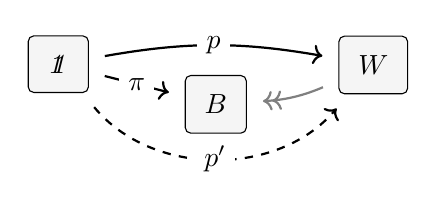
\begin{tikzpicture}[center base]
			% \useasboundingbox (-3,-1) rectangle (3.5,4);
			\node[dpadded] (1) at (0,0.51) {$\pdgunit$};
			\node[dpadded] (W) at (4,0.5) {$W$};
			\node[dpadded] (B) at (2,0) {$B$};
			% \node[dpadded] (E) at (6, 0.5 ){$E$};
			% \coordinate (Q) at (6,0); % to even out controls

			\draw[arr] (1) to[bend left=10] node[fill=white]{$p$} (W);
			\draw[arr] (1) to node[fill=white]{$\pi$} (B);

			\draw[arr, gray, ->>] (W) to[bend left=10] (B);
			% \draw[arr, dashed] (B) to[bend right=30] (W);	
			\draw[arr, dashed] (1) to[bend right=50] node[fill=white]{$p'$}(W);	
			% \draw[arr, ->>] (W) to (E);

			% \draw[arr,blue!50] (1) .. controls (2, -1) and (4,-1) .. node[fill=white]{$p'(E)$} (E);
			% \draw[arr,orange!70] (1) .. controls (2,2) and (4,2) .. node[fill=white]{$p(E)$} (E);
		\end{tikzpicture}}
		\caption{PDG Belief Updating via Inconsistency}
		\label{fig:belief-update}
	\end{figure}
}
%joe18: \end{commentout}
	% To understand the update visually
	% in \Cref{fig:belief-update}, imagine the original
	% distribution $p$ from $\sf 1$ to $W$ being replaced by the
	% path $p' := p(W \mid B) \circ \pi$  on the left. The gray
	% arrow on the bottom left is the definition of the random
	% variable, as in \Cref{ex:randomvars}, and the dashed one is
	% its inversion, which can be computed by Bayes' rule.  %that
	% factors through $B$ via the new observation $\pi$. 
	% To query the resulting distribution on, an arbitrary event $E$, with an indicator variable of the same name. Initially, we got a marginal on $E$ by going through $p$; we now use $p'$. Effectively, the orange path to $E$ has been replaced by the blue one.
	% 
	% 
	% To observe $\pi$, we simply view it as a cpd conditioned on $\star$ and add it to our collection. 
	% Although it is likely to be inconsistent, resolving this inconsistency in a way that retains $\pi$ is a belief update. 
	% Even failure retain $\pi$ entirely may not be a concern: so long as an they continue to observe or remember, an agent endures discomfort until $\pi$ is incorporated. This setting is arguably more natural than a standard one: without spending energy, it is easy to forget or partially reject implications of the observation.	
	% Once again, with a PDG, the resolution need not happen immediately. This makes the approach more convincing for cognitively bounded agents, who might have more pressing matters than sorting through beliefs, and who might do them out of order.
}%\end{commentout}
\vleftovers{
	\section{Algorithms} 
		\label{sec:algorithms}
	\subsection{Belief Propagation}
	
	
	\subsection{Sampling}
	
	One of the nice about directed graphical models is that the model itself is roughly a sampling algorithm. For instance, taking a Bayes Net $\cal B$ and generating samples according to the tables is an efficient way to sample $\Pr_{\mathcal B}$.

	This works because there is only one path, but more generally, for a conditional marginal $Y|X$, we can think of all of the different paths in the PDG different ways an agent with knowledge $\dg M$ can get probabilistic estimates of the conditional distribution $\bbr{\dg M}\MaxEnt(Y | X)$. The next result states that, in a precise sense, these various estimates bound the location of the marginal for this maximum entropy distribution, which suggests an efficient sampling algorithm for $\bbr{\dg M}\MaxEnt(Y | X)$, after learning some weights.
	
	\begin{conj}\label{thm:maxent-hull}
		For a PDG $\dg M = \pdgvars[]$ containing variables $X, Y$, the maximum entropy conditional marginal $\bbr{\dg M}\MaxEnt(y \mid x)$ is a convex mixture of the conditional marginals generated by the paths from $X$ to $Y$.  That is, there exist weights $\{\alpha_i \geq 0\}$ on the paths in $\dg M$ and a bias weight $\alpha_0$ with $\sum_i {\alpha_i} = 1$ and
		\[ \bbr{\dg M}\MaxEnt(Y \mid X) = \alpha_0 \  p^{\text{unif}}_Y \sum_{p \in \bbr{\dg M}_\lambda(X, Y)} \alpha_i (p_1 \circ \ldots \circ p_k) \]
		where $p^{\text{unif}}_Y$ is the uniform distribution on $Y$, and $\bbr{\dg M}_\lambda(X,Y)$ is the set of paths from $X$ to $Y$ generated by composition and Bayes Rule in $\dg M$. 
	\end{conj}

	One natural choice of these $\alpha$'s is the certainty scores for each edge, given by a weighted PDG, but we do not have a further formal results in this direction.
	Note that it is common for humans to make decisions in this way: to estimate whether something is realistic by following multiple chains of reasoning weighting them by strength of argument.
	
%	\begin{conj}
%		The conditional marginal of the maximum entropy distribution $\bbr{M}\MaxEnt(b \mid a)$ is in the convex hull of the compositions of paths $A \to B$. 
%	\end{conj}
}


%oli26: New Section on Inference. 
%joe25*: We don't have the space to make this a section, and our
%discussion doesn't deserve to be called a section.  I folded this
%into the discussion section.  (I also didn't understand what you
%wrote, but even if I had understood it, I would have moved it.)
% \section{Inference and Dynamics in a PDG} \label{sec:inference}

\section{Discussion}
\commentout{
	Given more computation, would your beliefs be more consistent? Or would you
	explore further, forming more extensive networks of them?
	The canonical picture of an idealized agent has always given the first
	answer, but this may not necessarily be the case.
}
 
%oli10: deleted the previous text, 
	% We have given the semantics of PDGs, a modeling framework that enables formal reasoning about this kind of mental state, and is strictly more expressive than the class of Bayesian Networks. The scoring semantics for fixed $\beta_L = \gamma = 1$ recovers the factor graph. The distribution given by a PDG, however is not generally this one, but rather one that is as consistent as possible with the supplied cpds.
	% 
	% The material covered in the present paper is only part of the picture. There are two very important generalizations that we plan to cover next. First, by minorly relaxing the definition of a cpd so that it doesn't need to provide a distribution for a special \texttt{null} value, we gain a huge amount of expressive power, allowing for simpler representations of events and partial knowledge.
 	% Second, while we have discussed what happens in the limit as $\gamma \to 0$, emphasizing the quantitative part of the PDG, there is also a rich story to be told about the qualitative half. Together with the modularity provided by the PDG, and the relaxation to strict PDGs, PDGs are able to function as causal models.
%joe9*: rewrote completely.  You have a few lines to say more.  It
%would also be good to squeeze in somewhere something about related
%work (e.g., perhaps dependency networks).
\commentout{
	PDGs are a powerful tool for representing local probabilistic information.
	Though represented by a graph, the edges are interpreted differently. Each
	edge alone determines a cpd, making PDGs formally analogous to a commutative
	diagram, instead of a flow-chart. A more familiar network can be obtained
	with the use of multi-tailed arrows. 

	PDGs have a parameterized semantics $[[ - ]]_\gamma$, which always
	generalizes Bayesian Networks, and precisely becomes a factor graph when
	$\gamma=1$.  This exposes an implicit trade-off between quantitative and
	qualitative data; the two behave very differently, but are unfortunately
	fused in a factor graph. Both qualitative and quantitative information can
	be inconsistent, although the former is less straightforward, this
	preliminary paper we focus on the quantitative limit.

	Incorporating new variables, data, or restricting to subgraphs
        of a PDG is simple, making it possible to construct one by
        simply throwing together some pre-trained statistical
        models. Moreover, in the quantitative limit, PDGs continue to
        have local meaning, in stark contrast with energy-based models
        such as factor graphs. As a result, PDGs are not only a
        flexible representation, but modular as well. 

	The most dramatic feature of PDGs is their ability to deal with
	inconsistency. A PDG can track conflicting information from different
	sources, and its semantics identify when this occurs, rather than quietly
	sweeping problems under the rug. As a result, a user may resolve
	inconsistency in multiple ways. Inconsistency can be dealt with by updating
	one or multiple tables, by introducing introducing or splitting variables,
	or even left unresolved as as one searches for clarification. The pain of
	inconsistency can be mitigated by expressing a decreased confidence, without
	altering any data. 
}

We have introduced PDGs, a powerful tool for representing
probabilistic information. 
They have a number of advantages over other
% they have a number of advantages of other
%joe22: why did you change this?  pdgs are not a ``probabilistic model''
%oli25: i changed it because "representation" requires another concept
% for me, in order to typecheck: what is it a representation /of/? 
%oli25: also, why are pdgs not probabilistic models? they're a modeling tool,
% and any specific pdg models <something involving the variables>, with 
% probabilistic information. what is a proabilisitic model?
%joe23: i don't think of bns or pdgs as probabilistic models.  i don't
%even use the term ``proabilistic model''.  to the extent that i would
%find it acceptable, i would use it a contrast to a deterministic
%model.  i could live with ``probabilistic graphical model'', which is
%at least relatively standard terminology.  in the hopes that will be
%an acceptable compromise, i've made he change
%graphical representations:
%probablisitic models.
probablisitic graphical models. 
\begin{itemize}
\item They allow us to capture inconsistency, including conflicting information
%joe29: This doeesn't make sense.   First, I don't knw what ``variable
%confidence'' means.  Second, it seems strange to express confidence
%in inconsistency. I just cut this, which is what is needed to get is
%down to 8 pages anyway.
%from multiple sources, and express variable confidence in
%	%oli26
%	% the information. 
%	it.
%joe30: changed as you would probably prefer.
from multiple sources with varying degrees of reliability.
\item 
	They are much more modular 
	%oli11: If modularity = flexibility + ability to break into local components with meaning, then I buy this.
	% If modularity = flexibility of adding things, it's only true for directed models; factor graphs are modular as hell but difficult to interpret and only have global meaning.
	than other representations; for example, we can combine information from two sources by simply taking the union of two
	PDGs, and it is easy to add new information (edges)
	%oli11: I want something simpler than "representational capacity" but
	%I can't think of what to say instead 
	%joe10: I odn't know what ``representational capacity'' means.
	%and representational capacity (nodes)
	and features (nodes) without affecting previously-received information.
	%oli11: I like what you have written, but my paragraph above says a
	%lot more. I'm trying to merge them to make it clearer. 
	%oli11: This local meaning is super important. It was in the equation,
	%but I keep not being able to show it directly; I'll try to re-word.  
	%joe10: we haven't even defined restrictions, nor have we explained
	%this point.  You can't bring it up out of the blue now!  After
	%starting to make changs, I just cut this sentence
	%oli12: we have now explained the point. I'm inserting a part of this
	%again.
	%joe11*: we have *not* empahsized the point.  Nowhere do we talk about
	%preserving local meanings of cpds, nor explained why this is important.
	%In addition to their flexibility (and unlike similarly flexible models
	%such factor graphs), PDGs are unique in also preserving the local
	%meanings of their cpds.  
	%oli13*: This is an important subtlety --- if by "modular" you mean
	% flexiblle, then factor graphs are in some sense better than PDGs (you don't
	% even need to normalize your factors!), but we have not time or space. 
	% I guess I have to drop it..
\commentout{
	In contrast to factor graphs, restrictions of PDGs continue to retain the same
	local commitment to the meanings of cpds in the restriction. As a result, PDGs
	exhibit both flexibility and locality, making them uniquely modular. 
}
\item They allow for a clean separation between quantitiatve information (the
	cpds and weights $\beta$) and more qualitative information contained by
	the graph structure (and the weights $\alpha$); this is captured by the
	terms $\Inc$ and $\IDef{}$ in our scoring function.
 %oli24:added 
%joe22*: I'm unhappy about this.  First, as I've said repeatedly, I
%don't view \alpha as any more ``qualitative'' than \beta.
%oli25*: we have to fix this problem right away. It very much is, and I don't 
% think we should be having a disagreement about this.
%joe23: whether we should or shouldn't, we obviously do.  
%joe22: Second, it highights something that's currently unmotivated (\alpha)
%oli25: this is fair. However, we do spend a lot time showing using 
% \gamma to trade off one half with the other, and I want to nod to
% the fact that a PDG allows you to distinguish (and maybe parenthetically: and
% model spearately,in a way that doesn't make \alpha a focus) qualitative and
% quantitative effects.
%joe23: Maybe in your head, you're nodding to that, and not
%making \alpha a focus.  But that's not what I get out of it as a
%reader, and I believe that I'm more representative than you are here.
%oli25: No change, but I want to insert something to this effect.
%Furthermore, the fact that a PDG has two sets of weights allow
%        a modeler to 
%	specify qualitative and quantitative information separately.
\item PDGs have (several) natural semantics; one of them allows us to
%joe25
%pick out a unique distribution. This, in turn, shows that PDGs
pick out a unique distribution.  Using this distrbution, PDGs
	can capture BNs and factor graphs.
%oli27: reinserting the second half of the punchline
In the latter case, a simple parameter shift in the corresponding PDG eliminates
arguably problematic behavior of a factor graph.
%joe25*: cut the rest of this, partly to save space, and partly
%because it fits in at beset awkwardly with the simple point ``PDGs
%can capture BNs and factor graphs''.
%, in the latter case by 
%%oli26: I want to convey that the parameters are a natural constant,
%%as opposed to being chosen for the particular factor graph. 
%% choosing appropriate parameters in the scoring rule.  
%weighting the two terms of the scoring function equally. 
%However, they also avoid some of the arguably 
%%oli26: can't decide between "unatural properties" and "problematic
%%behavior" 
%unnatural properties
%% problematic behavior
%of factor graphs
%%oli26 inserted
%for other parameter choices.
\end{itemize}

%joe25*: put material on inference here, starting with an apology.
% A graphical model needs an inference algorithm to be useful.
%%oli26: I might not want to say this, because we're giving an
%%exponential-memory 
%%	 algorithm, which is also immediate from BN semantics.
% Such algorithms (e.g., Belief Propagation) are typically are much more complex
% than the model's semantics, but PDGs have a particualrly complex semantics and
% are particularly good at expressing inconsistency.
%joe25: let's not worry about how it can be done.  (I actually don't
%think that either can be done ``with the semantics'', but let's not
%get into a discussion about that.)
%oli27: I'm sure what I have to say here can be done with the scoring
%function, % and I view that as hugely important: it shows that what
%we've covered here lays 
% the technical groundwork for these other issues. In any case, I'm going to 
% re-insert the concept but will will change the wording,
% in the hope that resolves your concern.
%Inference in a PDG is closely related to updating, both of which can
%be done with only the semantics described in this paper.

We have only scratched the surface of what can be done with PDGs here.
%oli27: slight rewrite. 
% Two major issues that clearly need to be tackled are inference in a
% PDG, and the dynamics of PDGs, specifically, how PDGs should be
% updated with new information and how inconsistency in a PDG should be resolved.
Two major issues that need to be tackled are inference and dynamics.
How should we query a PDG for probabilistic information? How should 
%joe26: PDGs are not agents
%a PDG respond to new information, and resolve its inconsistencies?
we modify a PDG in light of new information or to make it more consistent?
%oli27:
% It turns out that these issues are closely related.  
These issues turn out to be closely related.
%joe26*: I would prefer not to say this.  I don't think it's exactly
%true, and I don't see what we gain by saying it.
%and surprisingly entwined with PDG semantics.
%oli27:
% Due to space considerations, 
Due to space limitations, 
%oli27:
% we will need to defer a serious discussion of this issue to a forthcoming paper,
%joe26
%we will need to defer a serious discussion to a forthcoming paper,
%joe30: we talk about a forthcoming paper below; no need to repeat it.
%we defer a serious discussion to a forthcoming paper,
%and just briefly give some intuitions and examples here.
we just briefly give some intuitions and examples here.

%joe25
%Inference in a PDG is closely related to updating.
%For instance, suppose that we
Suppose that we want to compute the probability of $Y$ given $X$ in a PDG $\dg M$. 
%
%oli30*: slight restructing of all old material; hopefully this is no less
%	pallatable than the original.
For a cpd $p(Y|X)$, let $\dg M^{+p}$ be the PDG obtained
by associating $p$ with a new edge in $\dg M$ from $X$ to $Y$, with
$\alpha_p \!=\! 0$. We judge the quality of a candidate answer $p$ 
%joee29: you haven't told the reader what ``best possible score'' means
by the best possible score that $\dg M^{+p}$ gives to any distribution 
%joe29
%(its degree of inconsistency). It can be shown that the best answer is
(which we call the \emph{degree of inconsistency} of $\dg M^{+p}$). It
%jeo29: measures don't have answers.  
%can be shown that the best answer is  
%by this measure is $\bbr{\dg M}^*(Y\!\mid\! X)$.
can be shown that the deegree of inconsistency is minimized by
$\bbr{\dg M}^*(Y\!\mid\! X)$.
%joe29
%Moreover the inconsistency of $\dg M^{+p}$ is smooth and strongly convex,
%so optima can be computed by standard gradient methods.
Since the degree of inconsistency of $\dg M^{+p}$ is smooth and
strongly convex as a function of $p$,
we can compute its optimum values by standard gradient methods.
\commentout{
%joe25: PDGs don't have scores; distributions do
%answer $p(Y|X)$ may be judged via the best score of the PDG obtained
%with the best score in the PDG obtained
%oli27: fair enough, but in fixing a linguistic issue and rewriting it 
%	differently, you are now saying something entirely different, and less 
%	interesting; I suspect that committing to this change is part of why you
%	had trouble with the rest of what I wrote.
%joe26: I had trouble with what you wrote because I didn't understand it.
%oli27: Immediately below: your rewrite. Below that: the original, for ease
%	of comparison with the my modified version. 
%answer $p(Y \mid X)$ can be determined by considering the distribution
%with the best score in the PDG 
%answer $p(Y|X)$ may be judged via the best score of the PDG obtained
%joe26*: I'm sorry. I don't understand what it means to judge a
%candidate p by the best score of a PDG.  What you wrote simply
%doesn't make sense to me.  I tried to put what I thought you meant
%A candidate
%answer $p(Y \!\mid\! X)$ may be judged via the best possible score, of
%any distribution, 
%with respect to the PDG
%oli28: a key point is that we don't have to do it for each
%distribution, because it's convex. Also, it is both helpful and
%standard to include the 
%	source and target of the conditional distribution in the notation.
% For each distribution $p$, we consider the PDG 
We judge a candidate answer $p(Y \!\mid\! X)$ by the
%oli29: the equation you inserted is already at play here. I think it distracts
%	from the point, so I'm putting it in a footnote.
% inconsistency of the PDG
%joe28: badly placed footnote.  More importantly, looking at it again,
%you can't introduce 
%a new technical notion out of the blue here, and call it
%``inconsistency'', without explaining to the reader what's going on.
%inconsistency%
degree of \emph{inconsistency} 
of the PDG
%oli27: changing notation back to union; it's clearer, and does not
%conflict with 
% our other uses for a subscript.
%joe26*: Since we're talking about aesthetics, let me exercise my
%aesthetic jdugment: I think it's ugly.
%oli28: done, and M^+p looks better to me also. (Though it is the union of two
%		PDGs, and I was tryng to make the notation uniform).
%${\dg M} \cup p$ (obtained
%oli29: a comma
% ${\dg M}^{+p}$ obtained 
${\dg M}^{+p}$, obtained 
%joe25*: I don't understand the next line.  There's clearly a typo
%here.  I wrote what I thought you meant
%by adding $p$ an edge of $\dg M$ (with $\alpha_p=0$).
%oli27*: I meant something much simpler: just add the edge p in addition (but
%	 it has to have a corresponding \alpha = 0). THe typo was a missing "as". 
% by updating the PDG $\dg M$ by removing all edges from $X$ to $Y$ (and their
% labels), then adding an edge from $X$ to $Y$ labeled by the cpd $p$.
%joe26*: Sorry, the next line simply does not make sense.  Let me list
%the many problems: (1) Where are we adding the edge?  I assume that
%we're adding it from X to Y, but you have to say that.  (2) p is not
%an edge, but a distribution.  At best, it's the label of the edge
%that you've added from X to Y.  (3) What if there are 
%already edges with other labels from X to Y?  Do you keep them?
%(4) FInally, and this is the key point: Are you claiming that the
%probability of Y given X in M is p(Y|X) for the p such that M+p has
%he best score?  If so, you have to say that.  If not, then I simply don't see
%what any of this is telling you.  Bottom line: this *must* be
%rewritten and clarified.
%oli28: (1) that p is an edge from X to Y is implicit in its type p(Y|X).
%joe27: Maybe it's clear to you, but, trust me, there will be a
%significant fraction of readers to whom it's not clear.  You are not
%typical!  To take just one example, it wasn't clear to me!
% (2) Sure, but I don't see why the distinction is meaningful. There is no 
%	ambiguity in identifying edges with the cpds, and this is supposed to be
%	an illustration. I'd also be happy to be more explicit if we had more room, 
%	but I am certain that nobody will think twice about this, so
%	long as we introduce p as p(Y|X). 
%joe27: Oliver, after I told you that I found this confusing, I don't
%see how you can say ``nobody will think twice about this''!  I don't
%understand why you resist making things clearer to the reader?  
% (3) We leave any other edges exactly as they are (which is why I say nothing about them).
% (4) Yes, I am saying this. And I reiterated it explicitly in the next sentence:
%	"according to which $\bbr{\dg M}^*(Y \!\mid\! X)$ is optimal."
%joe26
%by adding $p$ as an edge of $\dg M$ with $\alpha_p\!\!=\!0$).
%by adding $p$ as an edge of $\dg M$ with $\alpha_p\!\!=\!0$%
%oli29:
% by adding an edge labeled $p$ from $X$ to $Y$ to $\dg M$ with $\alpha_p\!\!=\!0$. 
by associating $p$ with a new edge in $\dg M$ from $X$ to $Y$, with
%joe28: inserted footnote here, and rewrote it slightly.  I am very
%uncomfortable this, because we haven't really defined the notion of ``inconsistency''
$\alpha_p \!=\! 0$.
%joe28*: First, you can't bury this in a footnote.  Second, this is far
%too mysterious.  What does ``for fixed \gamma'' mean?  Where
%is \gamma coming from?   This is unacceptable.  
%\footnote{equal to $\inf_{\mu} \bbr{\dg M^{+p}}_{\gamma}(\mu)$ for
%fixed $\gamma$ (which is  $\inf_\mu \Inc_{\dg M^{+p}}(\mu)$ in the
%limit as $\gamma\rightarrow0$), although this example does not depend
%on $\gamma$.}
%oli30: let's leave the technical details alone, as we can't agree
% on how to present them. Removing this.
% Roughly speaking, we measure this inconsistency by the expression
% $\inf_\mu \Inc_{\dg M^{+p}}(\mu)$. 
%BEGIN_FOLD: comments
%oli28: pulling remainder of the idea from earlier in sentence
%joe27*: Rewrote.  What you said is completely opaque to me.  As a
%technical matter, you're ``best score'' below is missing a gamma.  Do
%you mean to let \gamma go to 0?
%, i.e., the best possible score $\bbr{\dg M^{+p}}(\mu)$ of any
%distribution $\mu$. 
%%
%joe25: cut; no room.  I also don't see why the scoring semantics
%provides a measure of inference quality.  I don't even know
%what a measure of inference quality would be.
%oli27: I'm confused. I'm defining this to be a measure of inference quality.
%	And I thought that was the whole point of what I wrote in the AAAI rebuttal?
%	I'm replacing "measure" (possible technical reading I don't want) with 
%	"metric" and eliminating the equation. 
% Thus, the scoring semantics \eqref{eqn:full-score} provides a measure
% of inference quality  
%joe27*: I recognize that all the words of the next sentence are
%English, and I understand eah word individually, but I have no clue
%what the sentence is saying.  What is ``a metric of answer quality''?
%Why do we care?
%but I simply can't understand it! 
%In this way, the scoring semantics provides a metric of answer quality,
%%oli27: discuss optimality
%according to which $\bbr{\dg M}^*(Y \!\mid\! X)$ is optimal. 
%oli27: adding sentence that says that the best choice of P is correct.
%oli26: oof
%joe25*: I don't understand wht the equation is saying, and why it's
%computing p(Y|X).  Nor do I have a clue of what \gamma has to do with
%anything.  My guess is that my confusion will reflect that of the
%typical reader.  I cut it, and rewrote the following line
%oli27*: The line you cut is indeed confusing. I even sent
%	you a separate email explaining this equation and why I needed to say it.
%	You told me not worry about notation, and so it remains ugly. 
%	I am frustrated that after that exchange, you neither understood nor 
%	recognized this equation.
%	\gamma was along for the ride because our semantics is parameterized, but so
%	long as we're writing a gesture rather than a paper, we can leave it out. 
%	this version just uses English, whish is a little vaguer but should be easier
%	to follow. 
% $$\mathit{score}_\gamma(p) := \mapsto \bbr{\dg M \cup
% p}_\gamma(\bbr{\dg M \cup p}_\gamma^*).$$ 
%joe25
%This is smooth and strongly convex in $p$, so we can (at the cost of
%oli27:
% The score of ${\dg M}_p$ is smooth and strongly convex in $p$, so we can
%joe27*: I have no idea what metric you're talking about
%This metric happens to be smooth and strongly convex, so we can
%joe25: I don't know where this is coming from.  If you want to say
%it, you have to explain it!
%(at the cost of exponential memory)
%oli27: Fair enough. I did expand on this in a parenthetical of the next sentence,
% but I guess most people read papers in order. 
%oli27: clarified parenthetical & replaced "best answer" with the symbols to drive
% home that this in fact a computation of inference.
% directly compute the best answer with standard gradient methods
%directly compute $\bbr{\dg M}^*(Y \!\mid\! X)$ with standard gradient methods
%joe27: I'm lost.  Exponential in what?   What joint distributions are
%you storing?   There's no point in making mysterious statements like this.
%(at the cost of exponential memory, to store joint distributions). 
%oli26: I'm worried that the above isn't all that helpful by itself.
%joe25: Since I don't understand the above at all, it's certainly not helpful.
% Even without adding p to M, we can stll optimize the score to get a distribution 
% distribution $\mu$, and in particular the data \mu(Y | X). In our presentation,
% to add p, we also need to give a cpd and \beta > 0 (which we haven't discussed)
% so really there's no point in adding $p$ to the PDG.  
%oli27: Adressing your two points: 
% (1) You're right that we can still optimize the score without adding p, but if
% 	we simply do this, we have just pointed to our semantics for inference. That is
%	why we have to include the bit you cut below, on approximating the function, for
%	this to be at all useful. Otherwise, there's nothing to say here.
% (2)  My construction is compatible with the presentation.  Beta is totally
%	unimportant so I didn't mention it (\beta = 1 works), and I defined p(Y|X) 
%	to be a cpd itself (it is a candidate answer to Pr(Y|X)). 
%
%oli26: That said, doing something like this is still worth saying if we also 
% suggest that the representation of the distribution can be compressed, and the
% scoring function can be approximated...  
%joe25: cut; no room and too mysterious
%oli27: Like I say above, we need to give some hint that this not an unnecessary
%	dance that could be avoided by simply computing the best distribution and 
%	doing infrence on it. I think this is true because now we have
%this metric  
%	of quality, which is amenable to approximation. The
%approximation is critical.
%joe27*: I do not understand what you said above.  This does seem like
%a complicated why of ocmputing [[M]^*(Y|X), so perhaps you have to
%justify why you're doing that in this convoluted way, but I don't see
%how anything yo'vesid does that.
%	Reinstating with modifications for clarity.
%oli27: insert adverb to emphasize that this is the important part
% To the extent that we can estimate
%joe27*: I am trusting you that the next sentence (which is what I
%presume you meant) is true.  Since I can't seem to get you to write
%an outline of a paper on inference, perhaps you could at least
%provide a formal proof of this claim.
%oli27: parenthetical no longer necessary now that we explaind wy exponential
% 	memory in the appropriate place.
%joe27*: I'm not sure where you think you ``explained'' exponential
%memory.  All I can say is that I have no clue of what you're talking
%about here.
%Nevertheless, to the extent that we can estimate it efficiently
%% (i.e., without computing the full joint distribution $\bbr{\dg M \cup
%% p}^*$ in the process)
%%oli27: parenthetical no longer necessary now that we explaind wy exponential
%% 	memory in the appropriate place.
%(e.g., with a neural network), we may draw inferences efficiently as well. 
%END_FOLD comments
%oli29: Shortening and pulling equation above. See comments above and below for context.
% It can be shown that the cpd $p$ that minimizes
%joe28*: A high priority will be to prove this in the coming weeks.
%Also note that it's not a mteric; no point in calling it one.
%oli30: I see what you're saying, and that's why I changed it to "metric" from
% 	"measure"; both have technical meanings that we don't particularly intend. 
%	But also in both cases there are other technical readings of both words that
%	are unproblematic.  
%It can be shown that the best cpd $p$ by this metric
It can be shown that the best cpd $p$ by this measure
%oli29: While this expression is accurate, it looks more complex than it has to be
%	and unnecessarily takes a stance the value of $\gamma$ (in this simple example,
%	it is true for all \gamma, and also in the limit).
%	If we do decide to stick with the limit as \gamma goes to 0, then
%	there is also a simpler expression for it: it's just the inconsistency of the
%	PDG, Inc({\dg M}^{+p}) := \inf_\mu Inc_{{\dg M}^{+p}}(\mu)$. 
%	I've moved it to a footnote and rewritten it in plain English.
% $\inf_{\mu}\lim_{\gamma \rightarrow 0} \bbr{\dg M^{+p}}_\gamma(\mu)$
is $\bbr{\dg M}^*(Y \!\mid\! X)$.
%oli29: It might not be immediately obvious that with the \inf and limit the
%	expression is smooth & strongly convex (though it is),
%	so I'm changing the word "since".  I am also changing the word
%	"expression",  as the expression is hidden in the footnote.
% Moreover, since the expression that we want to minimize is 
%joe29
%Moreover, the deginconsistency of $\dg M^{+p}$ happens to be
Moreover, the degree of inconsistency of $\dg M^{+p}$ is
smooth and strongly convex in $p$,
%oli29: inserted, to accommodate change in sentence structure
%joe28
%and so
so
 we  can
%oli29: ambiguous antecedent for "it"
% calculate it 
calculate the best cpd $p$
with standard gradient methods. 
}
%oli30: end comment
This approach is
inefficient as written (since it involves computing the full joint
distribution 
%oli29: typo & brackets
% $\bbr{{\dg M}^-p}^*$), 
$\bbr{{\dg M}^{+p}}^*$), 
% oli29: a little more precision about why
%joe28: undid change.  What you said may be precise, but I find it
%incomprehesnible.  
%joe28: I don't understand this.  Specifically, I have no clue of what
%a ``direct approximation'' is.
%but a direct approximation of our metric would bypass this step, enabling
%effient inference.
%oli30*: prposed compromise
% but we believe that good approximation methods will allow us to draw inferences efficiently.
%joe29: NO!  It's not even clear what you're approximating
%but a good approximation of the consistency of $\dg M^{+p}$
%would circumvent this, allowing us to draw inferences efficiently.
but we believe that standard approximation techniques will allow us to
draw inferences efficiently.

%joe25*: I have no clue of what you're trying to say in the next.
%What does it mean to fix p and optimize \dg M?  I assume that it's
%not M that you're trying to optimize, but it's score.  But even given
%that, I have no clue what's varying in the optimization process.  I
%cut this for now; we probably don't have the space in any case.
%oli27: Actually, it /is/ M that I'm trying to optimize. The cpd p has some
% parameterization, and so do the rest of the cpds in M. If rather than 
% modifiying the paramteters of p, we modify the parmeters of the
% other cpds, we are doing updating. I'm re-introducing this content with
% changes for clarity.
\commentout{
	If, rather than fixing $\dg M$ and optimizing $p$, we fix $p$ and optimize $\dg M$,
	this same proces corresponds to an update, rather than an inference. For instance, in
	the case where $X = \pdgunit$, an observation $Y\!=\!y$  can be added to
	$\dg M$ in the form of an edge $\ed{\delta_y}{\pdgunit}Y$, getting the
	(possibly inconsistent) PDG $\dg M'$. The distribution $\bbr{M'}^*$ turns out
	to be the result of conditioning $\bbr{\dg M}^*$ on $Y\!=\!y$.  
}
%oli27: rewritten version, with your writing below folded in. 
% 
%is a special case of it.  I cut it.  We can exlain it in the paper
%that I hope we'll write.  
%joe26*: Sorry, I still do not undrestand this at all.  What does it
%mean to fix p.  Is there an edge labeled p in M? 
%		[%oli28: No, but there is in M^+p. ]
%If so, is it an edge from X to Y?  So you're saying that you fix one of the many
%edges in M and vary all the others and this gives you an update?
%		[%oli28: I'm saying fix one of the cpds of M^+p (concretely, fix p).
%			Reducing the inconsistency by changing the other parameters, results 
%			in an update incorporating p (as the resulting PDG is now consistent 
%			with p). ]
%Which update does it give you?
%		[%oli28: I claim that if we use gradient descent to update parameters,
%			we can take this as the definition of the update, and justify it
%			by the fact that the resulting consistent PDG appropriately reproduces
%			conditioning, Jeffrey's rule, etc. ]		
%joe27: I didn't undrstand that at all.  I don't see how this can be taken to
%be a definition of update.
% I'm lost.  I can't begin to try to fix it, since I don't undrstand it.
% I also don't have the time for a lot of back and forth.  If we can't
% converge on something quickly, I strongly suggest that we go back to my
% original version, which I think is clear nd makes the point well.
%oli28:
%	I think your original version is also probematic and would require
%	some back and forth for us to converge. I'm not sure exactly
%	what needs to be done to make you happy here, but I'm adding one more line
%	to tie things together explicitly a the end and removing "other"
%joe27*: And, yet again, I do not understand the next sentence at
%all.  Nor do I see how the case that I do understand (conditioning).
%I cut it.
\commentout{
If, rather than fixing $\dg M$ and varying $p$, we fix $p$ and vary the
%oli28: removing "other", probably a source of confusion
% parameters the other cpds of $\dg M$, the same optimization computes an update,
parameters the cpds of $\dg M$, the same optimization computes an update
rather than an inference. For example, to condition on an observation $Y\!=\!y$, we
can add to $\dg M$ an edge $\pdgunit \tto Y$, whose cpd is the degenerate
distribution $\delta_y$, thereby obtaining the (possibly inconsistent)
PDG ${\dg 
M}_{Y=y}$.
}
%joe27: reinstating my version, which at least I understand, and
%I believe will be of interest and comprehensible to a typical
%reader.  THere's not point writing something that most readers won't
%undrstand.  Whatever it is you're trying to say can be explained
%carefully in the paper you're trying to write.  I encourage you to
%write it an exlain it.
%oli29: (silently reduced spacing of Y=y and fixed the typo "\var 0" -> "\pdgunit")
	To take another example,
	conditioning can be understood in terms of resolving inconsistencies
	in a PDG.  To condition on an observation $Y\!=\!y$, given a situation
	described by a PDG $\dg M$, we can add an edge 
	from $\pdgunit$ to $Y$ in $\dg M$, annoted with the cpd that gives
	probability 1 to $y$, to get the (possibly inconsistent) PDG
%oli29:  (added a strut to aid typesetting)
	$\vphantom{\raisebox{0.05em}{$\big|$}}$
%oli29: I like the + better, and it makes the parallel with the previous example clearer. 
% ${\dg M}_{Y=y}$.   The distribution $\bbr{{\dg M}_{Y=y}}^*$ turns out
%joe28: I'm not sure I agree with your aesthetic judgment, but I can
%live with it, provided we add the parens
%${\dg M}^{+\!Y\!=y}$.   The distribution $\bbr{{\dg M}^{+\!Y\!=y}}^*$ turns out
${\dg M}^{+(\!Y\!=y)}$.   The distribution $\bbr{{\dg M}^{+(\!Y\!=y)}}^*$ turns out
to be the result of conditioning $\bbr{\dg M}^*$ on $Y\!=\!y$.
%The distribution $\bbr{{\dg M}_{Y=y}}^*$
%turns out to be the result of conditioning $\bbr{\dg M}^*$ on $Y\!=\!y$%
%oli28
%%.
%joe27*: And yet again, I can't understand the next line at all.
%; by varying the cpds of $\dg M$ we may represent it consistently.
%oli27: remove paragraph break
%
%joe25
%One issue we hope to foucs on in the future is dynamics.
%oli26: overlap with the next sentence; cutting for space.
%% We believe that PDGs will prove a particularly
%% useful tool for examining how agents resolve inconsistency.
%oli26: I like the wording of what you wrote better, and the word "pervasive"
%in particular --- but I do think it's a framing. 
%joe25: reistated, since I cut what you added
%oli27: folded this into my version above. 
\commentout{
	To take another example,
	conditioning can be understood in terms of resolving inconsistencies
	in a PDG.  To condition on an observation $Y=y$, given a situation
	describedby a PDG $\dg M$, we can add an edge 
	from $\var 0$ to $Y$ in $\dg M$, annoted with the cpd that gives
	probability 0 to $y$, to get the (possibly inconsistent) PDG ${\dg
	M}_{Y=y}$.   The distribution $\bbr{{\dg M}_{Y=y}}^*$ turns out
	to be the result of conditioning $\bbr{\dg M}^*$ on $Y=y$.
}
%
%oli26: This paragraph is also much too wordy, and doesn't say much, 
% especially in light of the new discussion. Rewriting.
%joe25*: Yet again, i can't follow what you wrote.  It presuably
%follows from the paragraph above tha I coudln't follow.  Since we
%don't have the space for it.  I tried to write something that I could
%follow, that maintained some of the spirit of what you wrote.
%n
% For example, conditioning can be viewed as a way of resolving that
% inconsistency (as can other more general approaches to belief updating, such
% as Jeffrey's Rule \cite{Jeffrey68}; we know that this generalization is
% cleanly captured with  PDGs.
%joe25: cut Jeffrey's rule for now; no space.
%Inference and conditioning are among them, as illustrated
%in \cref{sec:inference}.
%oli27: somehow we found space again.
This account of conditioning generalizes
without modification to give Jeffrey's Rule \cite{Jeffrey68}, a more
general approach to belief updating. 

%oli26: fix spelling of "propagation" [reviewer #5].
%oli26: removing "naturally". Would like to alter sentence structure further,
% so that it doesn't repeat in the final section.
%% Belief propogation, too,  can be naturally regarded in this light: 
%joe25*: too mysterious, and not clear what the fact that message
%passing algorithms reduce inconsistency has to do with PDGs.  
%Belief propagation can also be regarded this way. 
%A collection of pseudomarginals are that correspond to factor and variable
%beliefs may be inconsistent, and messsage passing algorithms are greedy
%mechanisms for reducing this inconsistency \cite{wainwright2008graphical}.
%
%oli26: too wordy
% More distantly related tasks in other fields, such as variational inference in
% machine learning, can also be framed as inconsistency reduction. 
%%-- Variational inference can also be viewed in these terms: 
%joe25*: cut: what does this have to do with PDGs?
%Variational inference is an even clearer application of inconsistency
%resolution. 
%A VAE is in some sense an assertion that both
%a distribution and a variational approximation to it are both accurate;
%minimmizing the inconsistency between them is the learning task
%\cite{kingma2013autoencoding}. 
%oli26: insert paragraph break
% In all three of these examples, the objective 
% can be written as a sum of relative entropies, suggesting that we can apply
%joe25*: my attempt at replacing what you wrote.  We shoudl give
%references for belief propagation and variational inference
%oli27*: This paragraph breaks the flow a little so I imagine you will want
% to modify it. If you do, keep in mind that:
% (1) Variational inference is both an inference procedure similar in spirit
 %	to the inference scheme we just described, and an updating procedure.
% (2) It brings inconsistency back in explicitly, so it transitions to the
% 	final paragraph effectively.  
%joe26: what does it mean to be a ``model for variational inference?
%PDGs are also a natural model for variational inference. A
%oli28: It was "graphical model" but I shortened it and it became less useful.
%oli28: Removing "inference" as it is already in the name "variational inference"
% Issues of updating, inference, and inconsistency all arise in
%joe27
%Issues of updating and inconsistency arise in
Issues of updating and inconsistency also arise in
variational inference. A  
variational autoencoder \cite{kingma2013autoencoding}, for instance, 
is essentially three cpds: a prior $p(Z)$, a decoder $p(X \!\mid\! Z)$, and 
an encoder $q(Z \!\mid\! X)$. Because two cpds target $Z$ (and the cpds are 
%joe26
%inconsistent until fully trained) this situation cannot be represented
%with other 
inconsistent until fully trained), this situation
%oli28:
 % cannot be represented 
can be represented by PDGs but not
by other graphical models.
%oli28: remove paragraph break
%
%oli27: Cutting belief propogation details to make room for VaE details, which 
% I think are much more illustrative. 
% We believe that it should also be possible to capture belief propagation 
%%and variational inference
% by adding edges to a PDG and then choosing the
% distribution whose score minimizes the inconsistency in the resulting PDG.
%In each example, the solution is given by finding parameters that 
%minimize a PDG's inconsistency, suggesting that we can apply 
%%oli26:
% PDGs without modification to capture an incredibly broad range of tasks and resolve them in a uniform way.
%PDG semantics to capture and solve a broad range of tasks in a uniform way.
%oli27: I dislike the "as we have said" in the final sentence, but otherwise it
% looks good to me
% As we said, we hope to report further on the deep connection between
We hope to report further on the deep connection between
inference, updating, 
%oli27: tweak wording
% and dealing with inconsistency in PDGs 
%joe26
%and the resolution of inconsistency
and the resolution of inconsistency in PDGs
in future work.

%oli22: added
%joe20
%Finally, many standard algorithms for inference on graphical models 
%run out-of-the box on PDGs; we are also interested in characterizing their
%behavior and 
%providing alterations so that they yield resluts consistent with the semantics\
%oli24: this is a really weak way to end. I'm removing it.
% Although we have not considered computational issues here, many
% standard algorithms for inference on graphical models
% seem directly applicable to PDGs; we plan on investigating their
% behavior to see the extent to which they can be modified to yield
% results consistent with the semantics that
% we have provided.

%joe17* this does not belong in a paper on PDGs
\vleftovers{
		\subsection{Inconsistency} \label{sec:consistency-ethos}
	
		Believing a logically inconsistent formula can lead you to arbitrarily bad conclusions, having an infeasible set of constraints makes all answers you could give wrong, and having inconsistent preferences can lose you infinite money. We don't want to build inconsistent systems or agents with incoherent views of the world, and so, where possible, we design them so they cannot possibly be broken in this way. Suppose, for example, that we are trying to represent some quantity that must be a point on the unit circle. We could do it with an $x$ and $y$ coordinate, but this could be problematic because $x^2+ y^2$ might not be 1 --- it would be safer and harder to go awry if we parameterize it by an angle $\theta \in [0, 2\pi)$ instead. In the absence of performance benefits (like needing to regularly use the $y$-coordinate and not wanting to compute a sine), why would we take the first approach, introducing a potentially complex data-invariant, when we could avoid it?
		
		This line of thought, though common and defensible, is flawed if we are not perfectly confident in the design of both our system and the ways it can interact with the outside world. Using similar logic, we might ask ourselves: Why ask programmers for type annotations when all instructions are operationally well-defined at run-time?  Why use extra training data if there's already enough there to specify a function? Why estimate a quantity in two ways when they will yield different answers? Why repeat and rephrase your ideas when this could make you contradict yourself? Why write test cases when they could fail and make the project inconsistent? Why conduct an experiment if it could just end up contradicting your current knowledge?
		
		These questions may seem silly, but there is a satisfying information theoretic answer to all of them: redundancy, though costly, is the primary tool that we use to combat the possibility of being wrong. Maintaining data invariants can be expensive but provides diagnostic information; in the example above, settings of $x$ and $y$ that don't lie on the unit circle provide diagnostic information that something has gone wrong.
		In many cases, it is also possible to paper over problems by forcibly re-instating local data invariants: for instance, we could re-normalize any values of $x$ and $y$ (so long as $xy \neq 0$; we can chose an arbitrary point otherwise) at every step. While this would reduce inconsistency, it also hides red flags.
		
		Using a Bayesian Network to represent a probability distribution is like representing a circle with $\theta \in [0, 2\pi)$.
		By construction, the result must be a distribution, and nothing can possibly go wrong so long as we can always decide on exactly one distribution which is sufficient for our purposes.
		%	By construction, the result must be a point on the circle, and nothing can possibly go wrong so long as we're sure that we will always have exactly enough information to determine such a point (for instance, we could never be totally clueless about the point, or just know its $x$ coordinate).
		
		
		The process of mechanistically forcing invariants is homologous to the standard practice for factor graphs: practitioners will often just assume that the density it defines is normalizable, and either forcibly re-normalize or cleverly avoid computing the normalization constant while still assuming that one exists; behavior is usually left unspecified in the unlikely event that it is not defined or zero.
%joe17
}
	
%oli8: removing
% \subsection{A LIST OF PDG BENEFITS}\label{sec:list-of-benefits}
% \todo{Remove and refactor into appendix}
% \begin{enumerate}[nosep]
% 	\item PDGs can represent both over-constrained and under-constrained mental states. 
% 	\item In particular, they may be inconsistent, which gives agents using PDGs the qualitatively new kind of `epistemic modesty': the possibility of realizing that something is wrong with their beliefs.
% 	\item Many standard algorithms, including as belief propagation, conditioning, and belief revision, can be regarded as resolution of inconsistency.
% 	\item PDGs can emulate the functionality of other graphical graphical models.
% 	\item PDGs are more modular, making it much less invasive to combine, reduce, or partially interpret parts of the model, compared to alternatives.
% 	\item The modularity enables type-forming rules which can be used to implement deductive inference.
% 	\item The many standard ways of adding and eliminating variables provides an answer to the question, ``why these possible worlds?''
% 	\item Compared with a standard constraint satisfaction problem, individual components have of have limited impact on the semantics.
% 	\item The class of free energies defined by PDGs is strictly more expressive than those given by alternative graphical models.
% \end{enumerate} % trade-off: harder to analyze.
	
%oli26: addded page break back
\clearpage
{
    % \small
    % \bibliographystyle{alpha}
    \bibliography{allrefs,z,joe}        
}

\section*{Ethics Statement}
	% Authors are required to include a statement of the broader impact of their work, including its ethical
	% aspects and future societal consequences. Authors should discuss both positive and negative outcomes,
	% if any. For instance, authors should discuss a) who may benefit from this research, b) who may be
	% put at disadvantage from this research, c) what are the consequences of failure of the system, and d)
	% whether the task/method leverages biases in the data. If authors believe this is not applicable to them,
	% authors can simply state this
Because PDGs are a recent theoretical development, there is a lot of
guesswork in evaluating the impact. Here are two views of opposite polarity.

\subsection{Positive Impacts}
One can imagine many applications of enabling simple and coherent
aggregation of (possibly inconsistent) information. In particular we
can imagine using PDGs to build and interpret a communal and global
database of statistical models, in a way that may not only enable more
accurate predictions, but also highlights conflicts between
information.

%joe1: what does fairness have to do with any of the above or below?
%This could have a critical impact on the state of fairness.
This could have many benefits. Suppose, for instance, that two researchers train
models, but use datasets with different racial makeups. Rather than trying to
get an uninterpretable model to ``get it right'' the first time, we could simply
highlight any
such clashes and flag them for review.

Rather than trying to ensure fairness by design, which is both tricky and
costly, we envision an alternative: simply aggregate (conflicting) statistically
optimal results, and allow existing social structure to resolve conflicts,
rather than sending researchers to fiddle with loss functions until they look fair. 


\subsection{Negative Impacts}

We can also imagine less rosy outcomes. To the extent that PDGs can
model and reason with inconsistency, if we adopt the attitude that a PDG need
not wait until it is consistent to be used, it is not hard to imagine a world
where a PDG gives biased and
poorly-thought out conclusions. It is clear that PDGs need a great deal more
vetting before they can be used for such important purposes as
aggregating the world's statistical knowledge.

PDGs are powerful statistical models, but are by necessity semantically more
complicated than many existing methods. This will likely restrict their
accessibility. To mitigate this, we commit to making sure our work is widely
accessible to researchers of different
backgrounds.
\fi
%BEGIN_FOLD: appendix
\ifappendix
\appendix
\clearpage
\onecolumn
%
\def\year{2021}\relax
% File: formatting-instruction.tex

\documentclass[letterpaper]{article} % DO NOT CHANGE THIS
\usepackage[margin=1in]{geometry}
% \usepackage{aaai21} % DO NOT CHANGE THIS
\usepackage{times} % DO NOT CHANGE THIS
\usepackage{helvet} % DO NOT CHANGE THIS
\usepackage{courier} % DO NOT CHANGE THIS
\usepackage[hyphens]{url} % DO NOT CHANGE THIS
\usepackage{graphicx} % DO NOT CHANGE THIS
\urlstyle{rm} % DO NOT CHANGE THIS
\def\UrlFont{\rm} % DO NOT CHANGE THIS
\usepackage{graphicx} % DO NOT CHANGE THIS
\usepackage{natbib} % DO NOT CHANGE THIS OR ADD OPTIONS
\usepackage{caption} % DO NOT CHANGE THIS OR ADD OPTIONS
\frenchspacing % DO NOT CHANGE THIS
\setlength{\pdfpagewidth}{8.5in} % DO NOT CHANGE THIS
\setlength{\pdfpageheight}{11in} % DO NOT CHANGE THIS

\usepackage{tikz}
	\usetikzlibrary{positioning,fit,calc, decorations, arrows, shapes, shapes.geometric}
	\usetikzlibrary{backgrounds}
	\usetikzlibrary{patterns}
	\usetikzlibrary{cd}
	
	\pgfdeclaredecoration{arrows}{draw}{
		\state{draw}[width=\pgfdecoratedinputsegmentlength]{%
			\path [every arrow subpath/.try] \pgfextra{%
				\pgfpathmoveto{\pgfpointdecoratedinputsegmentfirst}%
				\pgfpathlineto{\pgfpointdecoratedinputsegmentlast}%
			};
	}}
	%%%%%%%%%%%%
	\tikzset{AmpRep/.style={ampersand replacement=\&}}
	\tikzset{center base/.style={baseline={([yshift=-.8ex]current bounding box.center)}}}
	\tikzset{paperfig/.style={center base,scale=0.9, every node/.style={transform shape}}}

	\tikzset{is bn/.style={background rectangle/.style={fill=blue!35,opacity=0.3, rounded corners=5},show background rectangle}}
	% Node Stylings
	\tikzset{dpadded/.style={rounded corners=2, inner sep=0.7em, draw, outer sep=0.3em, fill={black!50}, fill opacity=0.08, text opacity=1}}
	\tikzset{dpad0/.style={outer sep=0.05em, inner sep=0.3em, draw=gray!75, rounded corners=4, fill=black!08, fill opacity=1}}
	\tikzset{dpad/.style args={#1}{every matrix/.append style={nodes={dpadded, #1}}}}
	\tikzset{light pad/.style={outer sep=0.2em, inner sep=0.5em, draw=gray!50}}
		
	\tikzset{arr/.style={draw, ->, thick, shorten <=3pt, shorten >=3pt}}
	\tikzset{arr0/.style={draw, ->, thick, shorten <=0pt, shorten >=0pt}}
	\tikzset{arr1/.style={draw, ->, thick, shorten <=1pt, shorten >=1pt}}
	\tikzset{arr2/.style={draw, ->, thick, shorten <=2pt, shorten >=2pt}}
	\tikzset{archain/.style args={#1}{arr, every arrow subpath/.style={draw,arr, #1}, decoration=arrows, decorate}}


	\tikzset{fgnode/.style={dpadded,inner sep=0.6em, circle},
	factor/.style={light pad, fill=black}}	
	
	
	\newcommand\cmergearr[4]{
		\draw[arr,-] (#1) -- (#4) -- (#2);
		\draw[arr, shorten <=0] (#4) -- (#3);
	}
	\newcommand\mergearr[3]{
		\coordinate (center-#1#2#3) at (barycentric cs:#1=1,#2=1,#3=1.2);
		\cmergearr{#1}{#2}{#3}{center-#1#2#3}
	}
	\newcommand\cunmergearr[4]{
		\draw[arr,-, , shorten >=0] (#1) -- (#4);
		\draw[arr, shorten <=0] (#4) -- (#2);
		\draw[arr, shorten <=0] (#4) -- (#3);
	}
	\newcommand\unmergearr[3]{
		\coordinate (center-#1#2#3) at (barycentric cs:#1=1.2,#2=1,#3=1);
		\cunmergearr{#1}{#2}{#3}{center-#1#2#3}
	}

	
	\usetikzlibrary{matrix}
	\tikzset{toprule/.style={%
	        execute at end cell={%
	            \draw [line cap=rect,#1] 
	            (\tikzmatrixname-\the\pgfmatrixcurrentrow-\the\pgfmatrixcurrentcolumn.north west) -- (\tikzmatrixname-\the\pgfmatrixcurrentrow-\the\pgfmatrixcurrentcolumn.north east);%
	        }
	    },
	    bottomrule/.style={%
	        execute at end cell={%
	            \draw [line cap=rect,#1] (\tikzmatrixname-\the\pgfmatrixcurrentrow-\the\pgfmatrixcurrentcolumn.south west) -- (\tikzmatrixname-\the\pgfmatrixcurrentrow-\the\pgfmatrixcurrentcolumn.south east);%
	        }
	    },
	    leftrule/.style={%
	        execute at end cell={%
	            \draw [line cap=rect,#1] (\tikzmatrixname-\the\pgfmatrixcurrentrow-\the\pgfmatrixcurrentcolumn.north west) -- (\tikzmatrixname-\the\pgfmatrixcurrentrow-\the\pgfmatrixcurrentcolumn.south west);%
	        }
	    },
	    rightrule/.style={%
	        execute at end cell={%
	            \draw [line cap=rect,#1] (\tikzmatrixname-\the\pgfmatrixcurrentrow-\the\pgfmatrixcurrentcolumn.north east) -- (\tikzmatrixname-\the\pgfmatrixcurrentrow-\the\pgfmatrixcurrentcolumn.south east);%
	        }
	    },
	    table with head/.style={
		    matrix of nodes,
		    row sep=-\pgflinewidth,
		    column sep=-\pgflinewidth,
		    nodes={rectangle,minimum width=2.5em, outer sep=0pt},
		    row 1/.style={toprule=thick, bottomrule},
  	    }
	}
\newif\ifprecompiledfigs
\precompiledfigsfalse
% \precompiledfigstrue

\newif\ifexternalizefigures\externalizefiguresfalse

\newif\ifappendix\appendixtrue
\newif\ifbody\bodyfalse

\ifexternalizefigures\else
	\usetikzlibrary{external}
	\tikzexternalize[prefix=tikz/]  % activate!
	% \usepackage{etoolbox}
	%  \AtBeginEnvironment{tikzcd}{\tikzexternaldisable} %... except careful of tikzcd...
	%  \AtEndEnvironment{tikzcd}{\tikzexternalenable}
\fi
%END_FOLD


%BEGIN_FOLD: Theorems and Tools

\usepackage{booktabs}       % professional-quality tables
\usepackage{amsfonts}       % blackboard math symbols
\usepackage{nicefrac}       % compact symbols for 1/2, etc.
\usepackage{microtype}      % microtypography
\usepackage{mathtools}		%also loads amsmath
\usepackage{amssymb, bbm}

%oli20: oops, this is vorboten :(
% \usepackage[format=plain,
%             labelfont={sl},
%             textfont={it,small}]{caption}

\usepackage{relsize}
\usepackage{environ} % http://ctan.org/pkg/environ; for capturing body as a parameter for idxmats

\usepackage{color}
%\usepackage{stmaryrd}

\usepackage{amsthm}
\usepackage{thmtools}

\theoremstyle{plain}
\newtheorem{theorem}{Theorem}[section]
\newtheorem{coro}{Corollary}[theorem]
\newtheorem{prop}[theorem]{Proposition}
\newtheorem{lemma}[theorem]{Lemma}
\newtheorem{fact}[theorem]{Fact}
\newtheorem{conj}[theorem]{Conjecture}

\theoremstyle{definition}

% no section numbers for theorems in AAAI style ... 
%joe17: can you reinstate this?
%oli20:done
\declaretheorem[name=Definition,qed=$\square$,numberwithin=section]{defn} %
\declaretheorem[name=Construction,qed=$\square$,sibling=defn]{constr}
\declaretheorem[qed=$\square$]{example}

\theoremstyle{remark}
\newtheorem*{remark}{Remark}

\usepackage{xstring}
\usepackage{enumitem}

\usepackage{environ}
\usepackage{xstring}

% Wow this works I'm brilliant
\def\wrapwith#1[#2;#3]{
	\expandarg\IfSubStr{#1}{,}{
		\expandafter#2{\expandarg\StrBefore{#1}{,}}
		\expandarg\StrBehind{#1}{,}[\tmp]
		\xdef\tmp{\expandafter\unexpanded\expandafter{\tmp}}
		#3
		\wrapwith{\tmp}[#2;{#3}]
	}{ \expandafter#2{#1} }
}
\def\hwrapcells#1[#2]{\wrapwith#1[#2;&]}
\def\vwrapcells#1[#2]{\wrapwith#1[#2;\\]}
\NewEnviron{mymathenv}{$\BODY$}

\newcommand{\smalltext}[1]{\text{\footnotesize#1}}
\newsavebox{\idxmatsavebox}
\def\makeinvisibleidxstyle#1#2{\phantom{\hbox{#1#2}}}
\newenvironment{idxmatphant}[4][\color{gray}\smalltext]{%
	\def\idxstyle{#1}
	\def\colitems{#3}
	\def\rowitems{#2}
	\def\phantitems{#4}
	\begin{lrbox}{\idxmatsavebox}$%$\begin{mymathenv}
	\begin{matrix}  \begin{matrix} \hwrapcells{\colitems}[\idxstyle]  \end{matrix}
		% &\vphantom{\idxstyle\colitems}
		\\[-0.05em]
		\left[
		\begin{matrix}
			\hwrapcells{\phantitems}[\expandafter\makeinvisibleidxstyle\idxstyle]  \\[-1.2em]
	}{
		\end{matrix}\right]		&\hspace{-0.8em}\begin{matrix*}[l] \vwrapcells{\rowitems}[\idxstyle] \end{matrix*}\hspace{0.1em}%
	\end{matrix}%
	$%\end{mymathenv}
	\end{lrbox}%
	\raisebox{0.75em}{\usebox\idxmatsavebox}
%	\vspace{-0.5em}
}

\newenvironment{idxmat}[3][\color{gray}\smalltext]
	{\begingroup\idxmatphant[#1]{#2}{#3}{#3}}
	{\endidxmatphant\endgroup}

\newenvironment{sqidxmat}[2][\color{gray}\smalltext]
	{\begingroup\idxmat[#1]{#2}{#2}}
	{\endidxmat\endgroup}


%%%%%%%%%%%%
% better alignment for cases
\makeatletter
\renewenvironment{cases}[1][l]{\matrix@check\cases\env@cases{#1}}{\endarray\right.}
\def\env@cases#1{%
	\let\@ifnextchar\new@ifnextchar
	\left\lbrace\def\arraystretch{1.2}%
	\array{@{}#1@{\quad}l@{}}}
\makeatother

\newcommand\numberthis{\addtocounter{equation}{1}\tag{\theequation}}

%oli20: apparently this is not allowed in AAAI style.
%oli21: but it helps me edit so I'm reenabling it until later
%oli25:
% \usepackage{xr}
% \usepackage{xr-hyper}
\usepackage{zref-xr}
% \usepackage{hyperref}
\zxrsetup{toltxlabel=true, tozreflabel=false}
\zexternaldocument*{pdg}
%oli24: the time has come... goodbye links and colors :(
% \usepackage{hyperref}
% \definecolor{deepgreen}{rgb}{0,0.5,0}
% \hypersetup{colorlinks=true, linkcolor=blue!50!black, urlcolor=magenta, citecolor=deepgreen}

\usepackage[noabbrev,nameinlink,capitalize]{cleveref}
\crefname{example}{Example}{Examples}
\crefname{defn}{Definition}{Definitions}
\crefname{prop}{Proposition}{Propositions}
\crefname{constr}{Construction}{Constructions}
\crefname{conj}{Conjecture}{Conjectures}
\crefname{fact}{Fact}{Facts}
%\crefname{section}{\S\!}{\S\!}


\usepackage{float}
% \usepackage{subcaption}
\newcounter{subfigure}
	% \captionsetup[subfigure]{subrefformat=simple,labelformat=simple}
	\renewcommand\thesubfigure{\thefigure(\alph{subfigure})}
    
\newenvironment{old}[1]{\par\noindent{\bf \Cref{#1}.} \em \noindent}{\par\medskip}

%% Version of recall that pulls the savebox:
% \usepackage{xpatch}
% \makeatletter
% \xpatchcmd{\thmt@restatable}% Edit \thmt@restatable
%    {\csname #2\@xa\endcsname\ifx\@nx#1\@nx\else[{#1}]\fi}% Replace this code
%    % {\ifthmt@thisistheone\csname #2\@xa\endcsname\typeout{oiii[#1;#2\@xa;#3;\csname thmt@stored@#3\endcsname]}\ifx\@nx#1\@nx\else[#1]\fi\else\csname #2\@xa\endcsname\fi}% with this code
%    {\ifthmt@thisistheone\csname #2\@xa\endcsname\ifx\@nx#1\@nx\else[{#1}]\fi
%    \else\fi}
%    {\typeout{oii Success1?}}{\typeout{oiii failure1?}} % execute code for success/failure instances
% \xpatchcmd{\thmt@restatable}% Edit \thmt@restatable
%    {\csname end#2\endcsname}
%    {\ifthmt@thisistheone\csname end#2\endcsname\else\fi}
%    {\typeout{oii Success2?}}{\typeout{oiii failure2?}}
% \newcommand{\recall}[1]{\medskip\par\noindent{\bf \expandarg\Cref{thmt@@#1}.} \begingroup\em \noindent
%    \expandafter\csname#1\endcsname* \endgroup\par\smallskip}
% \makeatother

\newcommand{\restate}[2]
	{\medskip\par\noindent{\bf \expandarg\Cref{thmt@@#1}.}%
 	\noindent\begingroup\em #2 \endgroup\par\smallskip}


%oli16: The extra space was because there was extra space in the paragraph, not
%because this length was too big. By breaking arrays, everything will be better.
\allowdisplaybreaks

\newcommand{\begthm}[3][]{\begin{#2}[{name=#1},restate=#3,label=#3]}

%TODO
\newcommand{\createversion}[2][{gray}{0.75}]{
	\definecolor{v#2color}#1\relax
    \expandafter\xdef\csname v#2on\endcsname{%
		% \xdef\gamma{\tau}%
		% \expandafter\renewcommand\csname v#2\endcsname{ONN}%
		% \expandafter\xdef{\csname v#2on\endcsname}##{{\color{v##2color} #1}}
	}
	\expandafter\xdef\csname v#2off\endcsname{
	% 	\expandafter\newcommand\csname v #2\endcsname[1]{{\color{v ##2 color} #1}}
	}
}
\createversion{test}
% \vteston
%END_FOLD

%BEGIN_FOLD   %%%% Version knobs %%%%%. 
%oli20: your commenting system is better than the one based on comment package, 
% which is way more problematic than I thought.
% I'm killing it and refactoring all comments to be like yours. I'm not annotating
% everything I'm doing here but the result will be way clearer and less problematic.

\definecolor{vfullcolor}{gray}{0.7}
\newcommand\vfull[1]{{\color{vfullcolor} #1}}
\renewcommand\vfull[1]{} % disable vfull

\definecolor{vleftoverscolor}{gray}{0.85}
\newcommand{\vleftovers}[1]{{\color{vleftoverscolor} #1}} 
\renewcommand{\vleftovers}[1]{} %disable vleftovers

\definecolor{notationcolor}{rgb}{0.9,0.9,.9} 
\newcommand{\notation}[1]{{\color{notationcolor} #1}}
\renewcommand{\notation}[1]{\ignorespaces} % disable notation

\definecolor{contentiouscolor}{rgb}{0.7,0.3,.1} 
\newcommand{\commentout}[1]{\ignorespaces} 

% \newcommand{\contentious}[1]{
% 	\noindent\colorbox{red!10!white}{\parbox{\linewidth-3pt}{\color{red!10!black}#1}}}
% \newcommand{\valpha}[1]{%
% 	% \colorbox{red!10!white}
% 	{\color{red!10!black}{#1}}%
% }
% \newcommand{\valpha}[1]{{\color{red!80!black}#1}}
\newcommand{\valpha}[1]{#1}

%END_FOLD


%BEGIN_FOLD definitions
%BEGIN_FOLD %%%%%   general shorthand I use   %%%%%%%%%%%%%%%%%

%\usepackage{stmaryrd}
%\DeclarePairedDelimiter{\ccbr}{\lBrace}{\rBrace}
%\DeclarePairedDelimiter{\bbr}{\llbracket}{\rrbracket}
%\DeclarePairedDelimiter{\ppr}{\llparenthesis}{\rrparenthesis}

\DeclarePairedDelimiterX{\bbr}[1]{[}{]}{\mspace{-3.5mu}\delimsize[#1\delimsize]\mspace{-3.5mu}}
\DeclarePairedDelimiter{\norm}{\lVert}{\rVert}

\let\Horig\H
\let\H\relax
\DeclareMathOperator{\H}{\mathrm{H}} % Entropy
\DeclareMathOperator{\I}{\mathrm{I}} % Information
\DeclareMathOperator*{\Ex}{\mathbb{E}} % Expectation
\DeclareMathOperator*{\argmin}{arg\;min}
\newcommand{\CI}{\mathrel{\perp\mspace{-10mu}\perp}} % Conditional Independence
\newcommand\mat[1]{\mathbf{#1}}
\DeclarePairedDelimiterX{\infdivx}[2]{(}{)}{%
	#1\;\delimsize\|\;#2%
}
\newcommand{\thickD}{I\mkern-8muD}
\newcommand{\kldiv}{\thickD\infdivx}


\newcommand{\todo}[1]{{\color{red}\ \!\Large\smash{\textbf{[}}{\normalsize\textsc{todo:} #1}\ \!\smash{\textbf{]}}}}
\newcommand{\note}[1]{{\color{blue}\ \!\Large\smash{\textbf{[}}{\normalsize\textsc{note:} #1}\ \!\smash{\textbf{]}}}}



% SPACES
\newcommand\Set{\mathbb{S}\mathrm{et}}
\newcommand\FinSet{\mathbb{F}\mathrm{in}\mathrm{S}\mathrm{et}}
\newcommand\Meas{\mathbb{M}\mathrm{eas}}
\newcommand\two{\mathbbm 2}

%END_FOLD

%BEGIN_FOLD %%%%%    PDG-specific macros     %%%%%%%%%%%%%%%%
\DeclarePairedDelimiterXPP{\SD}[1]{}{[}{]}{_{\text{sd}}}{\mspace{-3.5mu}\delimsize[#1\delimsize]\mspace{-3.5mu}}
		
%\usepackage{stmaryrd}
%\newcommand{\none}{\varobslash}
\newcommand{\none}{\bullet}

\def\sheq{\!=\!}
\DeclareMathOperator\dcap{\mathop{\dot\cap}}
\newcommand{\tto}{\rightarrow\mathrel{\mspace{-15mu}}\rightarrow}

\newcommand{\bp}[1][L]{\mat{p}_{\!_{#1}\!}}
\newcommand{\V}{\mathcal V}
\newcommand{\N}{\mathcal N}
\newcommand{\Ed}{\mathcal E}
\newcommand{\pdgvars}[1][]{(\N#1, \Ed#1, \V#1, \mat p#1, \beta#1)}


\DeclareMathAlphabet{\mathdcal}{U}{dutchcal}{m}{n}
\DeclareMathAlphabet{\mathbdcal}{U}{dutchcal}{b}{n}
%joe1:out of curiousity, why not use \mathcal?  That's what you use
%for BNs.  Why do PDG use a different font?
\newcommand{\dg}[1]{\mathbdcal{#1}}
\newcommand{\var}[1]{\mathsf{#1}}
\newcommand\Pa{\mathbf{Pa}}

%oli20: better spacing
% \newcommand{\IDef}[1]{\mathit{IDef}_{#1}}
\newcommand{\IDef}[1]{\mathit{IDef}_{\!#1}}

\newcommand\Inc{\mathit{Inc}}
\newcommand{\PDGof}[1]{{\dg M}_{#1}}
%oli22: a macro for unweighted PDGs
\newcommand{\UPDGof}[1]{{\dg N}_{#1}}
\newcommand{\WFGof}[1]{\Psi_{{#1}}}
%oli22: and for unweighted ones
\newcommand{\FGof}[1]{\Phi_{{#1}}}
%oli22: want to refer to the variable graph
\newcommand{\Gr}{\mathcal G}
%oli22: Gibbs Free Energy conflicts with \mathcal G. Now it lives in 
% this macro.
\newcommand\GFE{\mathit{G\mkern-4mu F\mkern-4.5mu E}}
%oli22: Right now we're using (\N, \V) to refer to variables of a
% PDG. I think it's important to keep both \N and \V but am happy to change
% the way we combine them. Factored into a macro so it's easier to change.
\newcommand{\varsNV}[1][\N,\V]{(#1)}


% \makeatletter %Arguments: L, X, Y, \scriptscriptstyle, -1pt (for raisebox)
% \newcommand{\ed@helper}[5]{#2\!%
%   \overset{\smash{\mskip-5mu\raisebox{-1pt}{$\scriptscriptstyle
%         #1$}}}{\rightarrow}\! #3} 
% \makeatother

%oli22: the edge notation is now uniform. Choose between the following
% Default: display as "X -L-> Y" (leave uncommented).
\newcommand{\ed}[3]{#2\!%
  \overset{\smash{\mskip-5mu\raisebox{-1pt}{$\scriptscriptstyle
        #1$}}}{\rightarrow}\! #3} 
% Option: uncomment to display as  "L = (X,Y,\ell)" instead.
% \renewcommand{\ed}[3]{#2 = (#1,#3,\ell)} 
\newcommand{\alle}[1][L]{_{ \ed {#1}XY}}


\begin{document}
\appendix
\onecolumn
%
\def\year{2021}\relax
% File: formatting-instruction.tex

\documentclass[letterpaper]{article} % DO NOT CHANGE THIS
\usepackage[margin=1in]{geometry}
% \usepackage{aaai21} % DO NOT CHANGE THIS
\usepackage{times} % DO NOT CHANGE THIS
\usepackage{helvet} % DO NOT CHANGE THIS
\usepackage{courier} % DO NOT CHANGE THIS
\usepackage[hyphens]{url} % DO NOT CHANGE THIS
\usepackage{graphicx} % DO NOT CHANGE THIS
\urlstyle{rm} % DO NOT CHANGE THIS
\def\UrlFont{\rm} % DO NOT CHANGE THIS
\usepackage{graphicx} % DO NOT CHANGE THIS
\usepackage{natbib} % DO NOT CHANGE THIS OR ADD OPTIONS
\usepackage{caption} % DO NOT CHANGE THIS OR ADD OPTIONS
\frenchspacing % DO NOT CHANGE THIS
\setlength{\pdfpagewidth}{8.5in} % DO NOT CHANGE THIS
\setlength{\pdfpageheight}{11in} % DO NOT CHANGE THIS

\usepackage{tikz}
	\usetikzlibrary{positioning,fit,calc, decorations, arrows, shapes, shapes.geometric}
	\usetikzlibrary{backgrounds}
	\usetikzlibrary{patterns}
	\usetikzlibrary{cd}
	
	\pgfdeclaredecoration{arrows}{draw}{
		\state{draw}[width=\pgfdecoratedinputsegmentlength]{%
			\path [every arrow subpath/.try] \pgfextra{%
				\pgfpathmoveto{\pgfpointdecoratedinputsegmentfirst}%
				\pgfpathlineto{\pgfpointdecoratedinputsegmentlast}%
			};
	}}
	%%%%%%%%%%%%
	\tikzset{AmpRep/.style={ampersand replacement=\&}}
	\tikzset{center base/.style={baseline={([yshift=-.8ex]current bounding box.center)}}}
	\tikzset{paperfig/.style={center base,scale=0.9, every node/.style={transform shape}}}

	\tikzset{is bn/.style={background rectangle/.style={fill=blue!35,opacity=0.3, rounded corners=5},show background rectangle}}
	% Node Stylings
	\tikzset{dpadded/.style={rounded corners=2, inner sep=0.7em, draw, outer sep=0.3em, fill={black!50}, fill opacity=0.08, text opacity=1}}
	\tikzset{dpad0/.style={outer sep=0.05em, inner sep=0.3em, draw=gray!75, rounded corners=4, fill=black!08, fill opacity=1}}
	\tikzset{dpad/.style args={#1}{every matrix/.append style={nodes={dpadded, #1}}}}
	\tikzset{light pad/.style={outer sep=0.2em, inner sep=0.5em, draw=gray!50}}
		
	\tikzset{arr/.style={draw, ->, thick, shorten <=3pt, shorten >=3pt}}
	\tikzset{arr0/.style={draw, ->, thick, shorten <=0pt, shorten >=0pt}}
	\tikzset{arr1/.style={draw, ->, thick, shorten <=1pt, shorten >=1pt}}
	\tikzset{arr2/.style={draw, ->, thick, shorten <=2pt, shorten >=2pt}}
	\tikzset{archain/.style args={#1}{arr, every arrow subpath/.style={draw,arr, #1}, decoration=arrows, decorate}}


	\tikzset{fgnode/.style={dpadded,inner sep=0.6em, circle},
	factor/.style={light pad, fill=black}}	
	
	
	\newcommand\cmergearr[4]{
		\draw[arr,-] (#1) -- (#4) -- (#2);
		\draw[arr, shorten <=0] (#4) -- (#3);
	}
	\newcommand\mergearr[3]{
		\coordinate (center-#1#2#3) at (barycentric cs:#1=1,#2=1,#3=1.2);
		\cmergearr{#1}{#2}{#3}{center-#1#2#3}
	}
	\newcommand\cunmergearr[4]{
		\draw[arr,-, , shorten >=0] (#1) -- (#4);
		\draw[arr, shorten <=0] (#4) -- (#2);
		\draw[arr, shorten <=0] (#4) -- (#3);
	}
	\newcommand\unmergearr[3]{
		\coordinate (center-#1#2#3) at (barycentric cs:#1=1.2,#2=1,#3=1);
		\cunmergearr{#1}{#2}{#3}{center-#1#2#3}
	}

	
	\usetikzlibrary{matrix}
	\tikzset{toprule/.style={%
	        execute at end cell={%
	            \draw [line cap=rect,#1] 
	            (\tikzmatrixname-\the\pgfmatrixcurrentrow-\the\pgfmatrixcurrentcolumn.north west) -- (\tikzmatrixname-\the\pgfmatrixcurrentrow-\the\pgfmatrixcurrentcolumn.north east);%
	        }
	    },
	    bottomrule/.style={%
	        execute at end cell={%
	            \draw [line cap=rect,#1] (\tikzmatrixname-\the\pgfmatrixcurrentrow-\the\pgfmatrixcurrentcolumn.south west) -- (\tikzmatrixname-\the\pgfmatrixcurrentrow-\the\pgfmatrixcurrentcolumn.south east);%
	        }
	    },
	    leftrule/.style={%
	        execute at end cell={%
	            \draw [line cap=rect,#1] (\tikzmatrixname-\the\pgfmatrixcurrentrow-\the\pgfmatrixcurrentcolumn.north west) -- (\tikzmatrixname-\the\pgfmatrixcurrentrow-\the\pgfmatrixcurrentcolumn.south west);%
	        }
	    },
	    rightrule/.style={%
	        execute at end cell={%
	            \draw [line cap=rect,#1] (\tikzmatrixname-\the\pgfmatrixcurrentrow-\the\pgfmatrixcurrentcolumn.north east) -- (\tikzmatrixname-\the\pgfmatrixcurrentrow-\the\pgfmatrixcurrentcolumn.south east);%
	        }
	    },
	    table with head/.style={
		    matrix of nodes,
		    row sep=-\pgflinewidth,
		    column sep=-\pgflinewidth,
		    nodes={rectangle,minimum width=2.5em, outer sep=0pt},
		    row 1/.style={toprule=thick, bottomrule},
  	    }
	}
\newif\ifprecompiledfigs
\precompiledfigsfalse
% \precompiledfigstrue

\newif\ifexternalizefigures\externalizefiguresfalse

\newif\ifappendix\appendixtrue
\newif\ifbody\bodyfalse

\ifexternalizefigures\else
	\usetikzlibrary{external}
	\tikzexternalize[prefix=tikz/]  % activate!
	% \usepackage{etoolbox}
	%  \AtBeginEnvironment{tikzcd}{\tikzexternaldisable} %... except careful of tikzcd...
	%  \AtEndEnvironment{tikzcd}{\tikzexternalenable}
\fi
%END_FOLD


%BEGIN_FOLD: Theorems and Tools

\usepackage{booktabs}       % professional-quality tables
\usepackage{amsfonts}       % blackboard math symbols
\usepackage{nicefrac}       % compact symbols for 1/2, etc.
\usepackage{microtype}      % microtypography
\usepackage{mathtools}		%also loads amsmath
\usepackage{amssymb, bbm}

%oli20: oops, this is vorboten :(
% \usepackage[format=plain,
%             labelfont={sl},
%             textfont={it,small}]{caption}

\usepackage{relsize}
\usepackage{environ} % http://ctan.org/pkg/environ; for capturing body as a parameter for idxmats

\usepackage{color}
%\usepackage{stmaryrd}

\usepackage{amsthm}
\usepackage{thmtools}

\theoremstyle{plain}
\newtheorem{theorem}{Theorem}[section]
\newtheorem{coro}{Corollary}[theorem]
\newtheorem{prop}[theorem]{Proposition}
\newtheorem{lemma}[theorem]{Lemma}
\newtheorem{fact}[theorem]{Fact}
\newtheorem{conj}[theorem]{Conjecture}

\theoremstyle{definition}

% no section numbers for theorems in AAAI style ... 
%joe17: can you reinstate this?
%oli20:done
\declaretheorem[name=Definition,qed=$\square$,numberwithin=section]{defn} %
\declaretheorem[name=Construction,qed=$\square$,sibling=defn]{constr}
\declaretheorem[qed=$\square$]{example}

\theoremstyle{remark}
\newtheorem*{remark}{Remark}

\usepackage{xstring}
\usepackage{enumitem}

\usepackage{environ}
\usepackage{xstring}

% Wow this works I'm brilliant
\def\wrapwith#1[#2;#3]{
	\expandarg\IfSubStr{#1}{,}{
		\expandafter#2{\expandarg\StrBefore{#1}{,}}
		\expandarg\StrBehind{#1}{,}[\tmp]
		\xdef\tmp{\expandafter\unexpanded\expandafter{\tmp}}
		#3
		\wrapwith{\tmp}[#2;{#3}]
	}{ \expandafter#2{#1} }
}
\def\hwrapcells#1[#2]{\wrapwith#1[#2;&]}
\def\vwrapcells#1[#2]{\wrapwith#1[#2;\\]}
\NewEnviron{mymathenv}{$\BODY$}

\newcommand{\smalltext}[1]{\text{\footnotesize#1}}
\newsavebox{\idxmatsavebox}
\def\makeinvisibleidxstyle#1#2{\phantom{\hbox{#1#2}}}
\newenvironment{idxmatphant}[4][\color{gray}\smalltext]{%
	\def\idxstyle{#1}
	\def\colitems{#3}
	\def\rowitems{#2}
	\def\phantitems{#4}
	\begin{lrbox}{\idxmatsavebox}$%$\begin{mymathenv}
	\begin{matrix}  \begin{matrix} \hwrapcells{\colitems}[\idxstyle]  \end{matrix}
		% &\vphantom{\idxstyle\colitems}
		\\[-0.05em]
		\left[
		\begin{matrix}
			\hwrapcells{\phantitems}[\expandafter\makeinvisibleidxstyle\idxstyle]  \\[-1.2em]
	}{
		\end{matrix}\right]		&\hspace{-0.8em}\begin{matrix*}[l] \vwrapcells{\rowitems}[\idxstyle] \end{matrix*}\hspace{0.1em}%
	\end{matrix}%
	$%\end{mymathenv}
	\end{lrbox}%
	\raisebox{0.75em}{\usebox\idxmatsavebox}
%	\vspace{-0.5em}
}

\newenvironment{idxmat}[3][\color{gray}\smalltext]
	{\begingroup\idxmatphant[#1]{#2}{#3}{#3}}
	{\endidxmatphant\endgroup}

\newenvironment{sqidxmat}[2][\color{gray}\smalltext]
	{\begingroup\idxmat[#1]{#2}{#2}}
	{\endidxmat\endgroup}


%%%%%%%%%%%%
% better alignment for cases
\makeatletter
\renewenvironment{cases}[1][l]{\matrix@check\cases\env@cases{#1}}{\endarray\right.}
\def\env@cases#1{%
	\let\@ifnextchar\new@ifnextchar
	\left\lbrace\def\arraystretch{1.2}%
	\array{@{}#1@{\quad}l@{}}}
\makeatother

\newcommand\numberthis{\addtocounter{equation}{1}\tag{\theequation}}

%oli20: apparently this is not allowed in AAAI style.
%oli21: but it helps me edit so I'm reenabling it until later
%oli25:
% \usepackage{xr}
% \usepackage{xr-hyper}
\usepackage{zref-xr}
% \usepackage{hyperref}
\zxrsetup{toltxlabel=true, tozreflabel=false}
\zexternaldocument*{pdg}
%oli24: the time has come... goodbye links and colors :(
% \usepackage{hyperref}
% \definecolor{deepgreen}{rgb}{0,0.5,0}
% \hypersetup{colorlinks=true, linkcolor=blue!50!black, urlcolor=magenta, citecolor=deepgreen}

\usepackage[noabbrev,nameinlink,capitalize]{cleveref}
\crefname{example}{Example}{Examples}
\crefname{defn}{Definition}{Definitions}
\crefname{prop}{Proposition}{Propositions}
\crefname{constr}{Construction}{Constructions}
\crefname{conj}{Conjecture}{Conjectures}
\crefname{fact}{Fact}{Facts}
%\crefname{section}{\S\!}{\S\!}


\usepackage{float}
% \usepackage{subcaption}
\newcounter{subfigure}
	% \captionsetup[subfigure]{subrefformat=simple,labelformat=simple}
	\renewcommand\thesubfigure{\thefigure(\alph{subfigure})}
    
\newenvironment{old}[1]{\par\noindent{\bf \Cref{#1}.} \em \noindent}{\par\medskip}

%% Version of recall that pulls the savebox:
% \usepackage{xpatch}
% \makeatletter
% \xpatchcmd{\thmt@restatable}% Edit \thmt@restatable
%    {\csname #2\@xa\endcsname\ifx\@nx#1\@nx\else[{#1}]\fi}% Replace this code
%    % {\ifthmt@thisistheone\csname #2\@xa\endcsname\typeout{oiii[#1;#2\@xa;#3;\csname thmt@stored@#3\endcsname]}\ifx\@nx#1\@nx\else[#1]\fi\else\csname #2\@xa\endcsname\fi}% with this code
%    {\ifthmt@thisistheone\csname #2\@xa\endcsname\ifx\@nx#1\@nx\else[{#1}]\fi
%    \else\fi}
%    {\typeout{oii Success1?}}{\typeout{oiii failure1?}} % execute code for success/failure instances
% \xpatchcmd{\thmt@restatable}% Edit \thmt@restatable
%    {\csname end#2\endcsname}
%    {\ifthmt@thisistheone\csname end#2\endcsname\else\fi}
%    {\typeout{oii Success2?}}{\typeout{oiii failure2?}}
% \newcommand{\recall}[1]{\medskip\par\noindent{\bf \expandarg\Cref{thmt@@#1}.} \begingroup\em \noindent
%    \expandafter\csname#1\endcsname* \endgroup\par\smallskip}
% \makeatother

\newcommand{\restate}[2]
	{\medskip\par\noindent{\bf \expandarg\Cref{thmt@@#1}.}%
 	\noindent\begingroup\em #2 \endgroup\par\smallskip}


%oli16: The extra space was because there was extra space in the paragraph, not
%because this length was too big. By breaking arrays, everything will be better.
\allowdisplaybreaks

\newcommand{\begthm}[3][]{\begin{#2}[{name=#1},restate=#3,label=#3]}

%TODO
\newcommand{\createversion}[2][{gray}{0.75}]{
	\definecolor{v#2color}#1\relax
    \expandafter\xdef\csname v#2on\endcsname{%
		% \xdef\gamma{\tau}%
		% \expandafter\renewcommand\csname v#2\endcsname{ONN}%
		% \expandafter\xdef{\csname v#2on\endcsname}##{{\color{v##2color} #1}}
	}
	\expandafter\xdef\csname v#2off\endcsname{
	% 	\expandafter\newcommand\csname v #2\endcsname[1]{{\color{v ##2 color} #1}}
	}
}
\createversion{test}
% \vteston
%END_FOLD

%BEGIN_FOLD   %%%% Version knobs %%%%%. 
%oli20: your commenting system is better than the one based on comment package, 
% which is way more problematic than I thought.
% I'm killing it and refactoring all comments to be like yours. I'm not annotating
% everything I'm doing here but the result will be way clearer and less problematic.

\definecolor{vfullcolor}{gray}{0.7}
\newcommand\vfull[1]{{\color{vfullcolor} #1}}
\renewcommand\vfull[1]{} % disable vfull

\definecolor{vleftoverscolor}{gray}{0.85}
\newcommand{\vleftovers}[1]{{\color{vleftoverscolor} #1}} 
\renewcommand{\vleftovers}[1]{} %disable vleftovers

\definecolor{notationcolor}{rgb}{0.9,0.9,.9} 
\newcommand{\notation}[1]{{\color{notationcolor} #1}}
\renewcommand{\notation}[1]{\ignorespaces} % disable notation

\definecolor{contentiouscolor}{rgb}{0.7,0.3,.1} 
\newcommand{\commentout}[1]{\ignorespaces} 

% \newcommand{\contentious}[1]{
% 	\noindent\colorbox{red!10!white}{\parbox{\linewidth-3pt}{\color{red!10!black}#1}}}
% \newcommand{\valpha}[1]{%
% 	% \colorbox{red!10!white}
% 	{\color{red!10!black}{#1}}%
% }
% \newcommand{\valpha}[1]{{\color{red!80!black}#1}}
\newcommand{\valpha}[1]{#1}

%END_FOLD


%BEGIN_FOLD definitions
%BEGIN_FOLD %%%%%   general shorthand I use   %%%%%%%%%%%%%%%%%

%\usepackage{stmaryrd}
%\DeclarePairedDelimiter{\ccbr}{\lBrace}{\rBrace}
%\DeclarePairedDelimiter{\bbr}{\llbracket}{\rrbracket}
%\DeclarePairedDelimiter{\ppr}{\llparenthesis}{\rrparenthesis}

\DeclarePairedDelimiterX{\bbr}[1]{[}{]}{\mspace{-3.5mu}\delimsize[#1\delimsize]\mspace{-3.5mu}}
\DeclarePairedDelimiter{\norm}{\lVert}{\rVert}

\let\Horig\H
\let\H\relax
\DeclareMathOperator{\H}{\mathrm{H}} % Entropy
\DeclareMathOperator{\I}{\mathrm{I}} % Information
\DeclareMathOperator*{\Ex}{\mathbb{E}} % Expectation
\DeclareMathOperator*{\argmin}{arg\;min}
\newcommand{\CI}{\mathrel{\perp\mspace{-10mu}\perp}} % Conditional Independence
\newcommand\mat[1]{\mathbf{#1}}
\DeclarePairedDelimiterX{\infdivx}[2]{(}{)}{%
	#1\;\delimsize\|\;#2%
}
\newcommand{\thickD}{I\mkern-8muD}
\newcommand{\kldiv}{\thickD\infdivx}


\newcommand{\todo}[1]{{\color{red}\ \!\Large\smash{\textbf{[}}{\normalsize\textsc{todo:} #1}\ \!\smash{\textbf{]}}}}
\newcommand{\note}[1]{{\color{blue}\ \!\Large\smash{\textbf{[}}{\normalsize\textsc{note:} #1}\ \!\smash{\textbf{]}}}}



% SPACES
\newcommand\Set{\mathbb{S}\mathrm{et}}
\newcommand\FinSet{\mathbb{F}\mathrm{in}\mathrm{S}\mathrm{et}}
\newcommand\Meas{\mathbb{M}\mathrm{eas}}
\newcommand\two{\mathbbm 2}

%END_FOLD

%BEGIN_FOLD %%%%%    PDG-specific macros     %%%%%%%%%%%%%%%%
\DeclarePairedDelimiterXPP{\SD}[1]{}{[}{]}{_{\text{sd}}}{\mspace{-3.5mu}\delimsize[#1\delimsize]\mspace{-3.5mu}}
		
%\usepackage{stmaryrd}
%\newcommand{\none}{\varobslash}
\newcommand{\none}{\bullet}

\def\sheq{\!=\!}
\DeclareMathOperator\dcap{\mathop{\dot\cap}}
\newcommand{\tto}{\rightarrow\mathrel{\mspace{-15mu}}\rightarrow}

\newcommand{\bp}[1][L]{\mat{p}_{\!_{#1}\!}}
\newcommand{\V}{\mathcal V}
\newcommand{\N}{\mathcal N}
\newcommand{\Ed}{\mathcal E}
\newcommand{\pdgvars}[1][]{(\N#1, \Ed#1, \V#1, \mat p#1, \beta#1)}


\DeclareMathAlphabet{\mathdcal}{U}{dutchcal}{m}{n}
\DeclareMathAlphabet{\mathbdcal}{U}{dutchcal}{b}{n}
%joe1:out of curiousity, why not use \mathcal?  That's what you use
%for BNs.  Why do PDG use a different font?
\newcommand{\dg}[1]{\mathbdcal{#1}}
\newcommand{\var}[1]{\mathsf{#1}}
\newcommand\Pa{\mathbf{Pa}}

%oli20: better spacing
% \newcommand{\IDef}[1]{\mathit{IDef}_{#1}}
\newcommand{\IDef}[1]{\mathit{IDef}_{\!#1}}

\newcommand\Inc{\mathit{Inc}}
\newcommand{\PDGof}[1]{{\dg M}_{#1}}
%oli22: a macro for unweighted PDGs
\newcommand{\UPDGof}[1]{{\dg N}_{#1}}
\newcommand{\WFGof}[1]{\Psi_{{#1}}}
%oli22: and for unweighted ones
\newcommand{\FGof}[1]{\Phi_{{#1}}}
%oli22: want to refer to the variable graph
\newcommand{\Gr}{\mathcal G}
%oli22: Gibbs Free Energy conflicts with \mathcal G. Now it lives in 
% this macro.
\newcommand\GFE{\mathit{G\mkern-4mu F\mkern-4.5mu E}}
%oli22: Right now we're using (\N, \V) to refer to variables of a
% PDG. I think it's important to keep both \N and \V but am happy to change
% the way we combine them. Factored into a macro so it's easier to change.
\newcommand{\varsNV}[1][\N,\V]{(#1)}


% \makeatletter %Arguments: L, X, Y, \scriptscriptstyle, -1pt (for raisebox)
% \newcommand{\ed@helper}[5]{#2\!%
%   \overset{\smash{\mskip-5mu\raisebox{-1pt}{$\scriptscriptstyle
%         #1$}}}{\rightarrow}\! #3} 
% \makeatother

%oli22: the edge notation is now uniform. Choose between the following
% Default: display as "X -L-> Y" (leave uncommented).
\newcommand{\ed}[3]{#2\!%
  \overset{\smash{\mskip-5mu\raisebox{-1pt}{$\scriptscriptstyle
        #1$}}}{\rightarrow}\! #3} 
% Option: uncomment to display as  "L = (X,Y,\ell)" instead.
% \renewcommand{\ed}[3]{#2 = (#1,#3,\ell)} 
\newcommand{\alle}[1][L]{_{ \ed {#1}XY}}


\begin{document}
\appendix
\onecolumn
%
\def\year{2021}\relax
% File: formatting-instruction.tex

\documentclass[letterpaper]{article} % DO NOT CHANGE THIS
\usepackage[margin=1in]{geometry}
% \usepackage{aaai21} % DO NOT CHANGE THIS
\usepackage{times} % DO NOT CHANGE THIS
\usepackage{helvet} % DO NOT CHANGE THIS
\usepackage{courier} % DO NOT CHANGE THIS
\usepackage[hyphens]{url} % DO NOT CHANGE THIS
\usepackage{graphicx} % DO NOT CHANGE THIS
\urlstyle{rm} % DO NOT CHANGE THIS
\def\UrlFont{\rm} % DO NOT CHANGE THIS
\usepackage{graphicx} % DO NOT CHANGE THIS
\usepackage{natbib} % DO NOT CHANGE THIS OR ADD OPTIONS
\usepackage{caption} % DO NOT CHANGE THIS OR ADD OPTIONS
\frenchspacing % DO NOT CHANGE THIS
\setlength{\pdfpagewidth}{8.5in} % DO NOT CHANGE THIS
\setlength{\pdfpageheight}{11in} % DO NOT CHANGE THIS

\usepackage{tikz}
	\usetikzlibrary{positioning,fit,calc, decorations, arrows, shapes, shapes.geometric}
	\usetikzlibrary{backgrounds}
	\usetikzlibrary{patterns}
	\usetikzlibrary{cd}
	
	\pgfdeclaredecoration{arrows}{draw}{
		\state{draw}[width=\pgfdecoratedinputsegmentlength]{%
			\path [every arrow subpath/.try] \pgfextra{%
				\pgfpathmoveto{\pgfpointdecoratedinputsegmentfirst}%
				\pgfpathlineto{\pgfpointdecoratedinputsegmentlast}%
			};
	}}
	%%%%%%%%%%%%
	\tikzset{AmpRep/.style={ampersand replacement=\&}}
	\tikzset{center base/.style={baseline={([yshift=-.8ex]current bounding box.center)}}}
	\tikzset{paperfig/.style={center base,scale=0.9, every node/.style={transform shape}}}

	\tikzset{is bn/.style={background rectangle/.style={fill=blue!35,opacity=0.3, rounded corners=5},show background rectangle}}
	% Node Stylings
	\tikzset{dpadded/.style={rounded corners=2, inner sep=0.7em, draw, outer sep=0.3em, fill={black!50}, fill opacity=0.08, text opacity=1}}
	\tikzset{dpad0/.style={outer sep=0.05em, inner sep=0.3em, draw=gray!75, rounded corners=4, fill=black!08, fill opacity=1}}
	\tikzset{dpad/.style args={#1}{every matrix/.append style={nodes={dpadded, #1}}}}
	\tikzset{light pad/.style={outer sep=0.2em, inner sep=0.5em, draw=gray!50}}
		
	\tikzset{arr/.style={draw, ->, thick, shorten <=3pt, shorten >=3pt}}
	\tikzset{arr0/.style={draw, ->, thick, shorten <=0pt, shorten >=0pt}}
	\tikzset{arr1/.style={draw, ->, thick, shorten <=1pt, shorten >=1pt}}
	\tikzset{arr2/.style={draw, ->, thick, shorten <=2pt, shorten >=2pt}}
	\tikzset{archain/.style args={#1}{arr, every arrow subpath/.style={draw,arr, #1}, decoration=arrows, decorate}}


	\tikzset{fgnode/.style={dpadded,inner sep=0.6em, circle},
	factor/.style={light pad, fill=black}}	
	
	
	\newcommand\cmergearr[4]{
		\draw[arr,-] (#1) -- (#4) -- (#2);
		\draw[arr, shorten <=0] (#4) -- (#3);
	}
	\newcommand\mergearr[3]{
		\coordinate (center-#1#2#3) at (barycentric cs:#1=1,#2=1,#3=1.2);
		\cmergearr{#1}{#2}{#3}{center-#1#2#3}
	}
	\newcommand\cunmergearr[4]{
		\draw[arr,-, , shorten >=0] (#1) -- (#4);
		\draw[arr, shorten <=0] (#4) -- (#2);
		\draw[arr, shorten <=0] (#4) -- (#3);
	}
	\newcommand\unmergearr[3]{
		\coordinate (center-#1#2#3) at (barycentric cs:#1=1.2,#2=1,#3=1);
		\cunmergearr{#1}{#2}{#3}{center-#1#2#3}
	}

	
	\usetikzlibrary{matrix}
	\tikzset{toprule/.style={%
	        execute at end cell={%
	            \draw [line cap=rect,#1] 
	            (\tikzmatrixname-\the\pgfmatrixcurrentrow-\the\pgfmatrixcurrentcolumn.north west) -- (\tikzmatrixname-\the\pgfmatrixcurrentrow-\the\pgfmatrixcurrentcolumn.north east);%
	        }
	    },
	    bottomrule/.style={%
	        execute at end cell={%
	            \draw [line cap=rect,#1] (\tikzmatrixname-\the\pgfmatrixcurrentrow-\the\pgfmatrixcurrentcolumn.south west) -- (\tikzmatrixname-\the\pgfmatrixcurrentrow-\the\pgfmatrixcurrentcolumn.south east);%
	        }
	    },
	    leftrule/.style={%
	        execute at end cell={%
	            \draw [line cap=rect,#1] (\tikzmatrixname-\the\pgfmatrixcurrentrow-\the\pgfmatrixcurrentcolumn.north west) -- (\tikzmatrixname-\the\pgfmatrixcurrentrow-\the\pgfmatrixcurrentcolumn.south west);%
	        }
	    },
	    rightrule/.style={%
	        execute at end cell={%
	            \draw [line cap=rect,#1] (\tikzmatrixname-\the\pgfmatrixcurrentrow-\the\pgfmatrixcurrentcolumn.north east) -- (\tikzmatrixname-\the\pgfmatrixcurrentrow-\the\pgfmatrixcurrentcolumn.south east);%
	        }
	    },
	    table with head/.style={
		    matrix of nodes,
		    row sep=-\pgflinewidth,
		    column sep=-\pgflinewidth,
		    nodes={rectangle,minimum width=2.5em, outer sep=0pt},
		    row 1/.style={toprule=thick, bottomrule},
  	    }
	}
\newif\ifprecompiledfigs
\precompiledfigsfalse
% \precompiledfigstrue

\newif\ifexternalizefigures\externalizefiguresfalse

\newif\ifappendix\appendixtrue
\newif\ifbody\bodyfalse

\ifexternalizefigures\else
	\usetikzlibrary{external}
	\tikzexternalize[prefix=tikz/]  % activate!
	% \usepackage{etoolbox}
	%  \AtBeginEnvironment{tikzcd}{\tikzexternaldisable} %... except careful of tikzcd...
	%  \AtEndEnvironment{tikzcd}{\tikzexternalenable}
\fi
%END_FOLD


%BEGIN_FOLD: Theorems and Tools

\usepackage{booktabs}       % professional-quality tables
\usepackage{amsfonts}       % blackboard math symbols
\usepackage{nicefrac}       % compact symbols for 1/2, etc.
\usepackage{microtype}      % microtypography
\usepackage{mathtools}		%also loads amsmath
\usepackage{amssymb, bbm}

%oli20: oops, this is vorboten :(
% \usepackage[format=plain,
%             labelfont={sl},
%             textfont={it,small}]{caption}

\usepackage{relsize}
\usepackage{environ} % http://ctan.org/pkg/environ; for capturing body as a parameter for idxmats

\usepackage{color}
%\usepackage{stmaryrd}

\usepackage{amsthm}
\usepackage{thmtools}

\theoremstyle{plain}
\newtheorem{theorem}{Theorem}[section]
\newtheorem{coro}{Corollary}[theorem]
\newtheorem{prop}[theorem]{Proposition}
\newtheorem{lemma}[theorem]{Lemma}
\newtheorem{fact}[theorem]{Fact}
\newtheorem{conj}[theorem]{Conjecture}

\theoremstyle{definition}

% no section numbers for theorems in AAAI style ... 
%joe17: can you reinstate this?
%oli20:done
\declaretheorem[name=Definition,qed=$\square$,numberwithin=section]{defn} %
\declaretheorem[name=Construction,qed=$\square$,sibling=defn]{constr}
\declaretheorem[qed=$\square$]{example}

\theoremstyle{remark}
\newtheorem*{remark}{Remark}

\usepackage{xstring}
\usepackage{enumitem}

\input{labelmatrix.tex}
\newcommand\numberthis{\addtocounter{equation}{1}\tag{\theequation}}

%oli20: apparently this is not allowed in AAAI style.
%oli21: but it helps me edit so I'm reenabling it until later
%oli25:
% \usepackage{xr}
% \usepackage{xr-hyper}
\usepackage{zref-xr}
% \usepackage{hyperref}
\zxrsetup{toltxlabel=true, tozreflabel=false}
\zexternaldocument*{pdg}
%oli24: the time has come... goodbye links and colors :(
% \usepackage{hyperref}
% \definecolor{deepgreen}{rgb}{0,0.5,0}
% \hypersetup{colorlinks=true, linkcolor=blue!50!black, urlcolor=magenta, citecolor=deepgreen}

\usepackage[noabbrev,nameinlink,capitalize]{cleveref}
\crefname{example}{Example}{Examples}
\crefname{defn}{Definition}{Definitions}
\crefname{prop}{Proposition}{Propositions}
\crefname{constr}{Construction}{Constructions}
\crefname{conj}{Conjecture}{Conjectures}
\crefname{fact}{Fact}{Facts}
%\crefname{section}{\S\!}{\S\!}


\usepackage{float}
% \usepackage{subcaption}
\newcounter{subfigure}
	% \captionsetup[subfigure]{subrefformat=simple,labelformat=simple}
	\renewcommand\thesubfigure{\thefigure(\alph{subfigure})}
    
\newenvironment{old}[1]{\par\noindent{\bf \Cref{#1}.} \em \noindent}{\par\medskip}

%% Version of recall that pulls the savebox:
% \usepackage{xpatch}
% \makeatletter
% \xpatchcmd{\thmt@restatable}% Edit \thmt@restatable
%    {\csname #2\@xa\endcsname\ifx\@nx#1\@nx\else[{#1}]\fi}% Replace this code
%    % {\ifthmt@thisistheone\csname #2\@xa\endcsname\typeout{oiii[#1;#2\@xa;#3;\csname thmt@stored@#3\endcsname]}\ifx\@nx#1\@nx\else[#1]\fi\else\csname #2\@xa\endcsname\fi}% with this code
%    {\ifthmt@thisistheone\csname #2\@xa\endcsname\ifx\@nx#1\@nx\else[{#1}]\fi
%    \else\fi}
%    {\typeout{oii Success1?}}{\typeout{oiii failure1?}} % execute code for success/failure instances
% \xpatchcmd{\thmt@restatable}% Edit \thmt@restatable
%    {\csname end#2\endcsname}
%    {\ifthmt@thisistheone\csname end#2\endcsname\else\fi}
%    {\typeout{oii Success2?}}{\typeout{oiii failure2?}}
% \newcommand{\recall}[1]{\medskip\par\noindent{\bf \expandarg\Cref{thmt@@#1}.} \begingroup\em \noindent
%    \expandafter\csname#1\endcsname* \endgroup\par\smallskip}
% \makeatother

\newcommand{\restate}[2]
	{\medskip\par\noindent{\bf \expandarg\Cref{thmt@@#1}.}%
 	\noindent\begingroup\em #2 \endgroup\par\smallskip}


%oli16: The extra space was because there was extra space in the paragraph, not
%because this length was too big. By breaking arrays, everything will be better.
\allowdisplaybreaks

\newcommand{\begthm}[3][]{\begin{#2}[{name=#1},restate=#3,label=#3]}

%TODO
\newcommand{\createversion}[2][{gray}{0.75}]{
	\definecolor{v#2color}#1\relax
    \expandafter\xdef\csname v#2on\endcsname{%
		% \xdef\gamma{\tau}%
		% \expandafter\renewcommand\csname v#2\endcsname{ONN}%
		% \expandafter\xdef{\csname v#2on\endcsname}##{{\color{v##2color} #1}}
	}
	\expandafter\xdef\csname v#2off\endcsname{
	% 	\expandafter\newcommand\csname v #2\endcsname[1]{{\color{v ##2 color} #1}}
	}
}
\createversion{test}
% \vteston
%END_FOLD

%BEGIN_FOLD   %%%% Version knobs %%%%%. 
%oli20: your commenting system is better than the one based on comment package, 
% which is way more problematic than I thought.
% I'm killing it and refactoring all comments to be like yours. I'm not annotating
% everything I'm doing here but the result will be way clearer and less problematic.

\definecolor{vfullcolor}{gray}{0.7}
\newcommand\vfull[1]{{\color{vfullcolor} #1}}
\renewcommand\vfull[1]{} % disable vfull

\definecolor{vleftoverscolor}{gray}{0.85}
\newcommand{\vleftovers}[1]{{\color{vleftoverscolor} #1}} 
\renewcommand{\vleftovers}[1]{} %disable vleftovers

\definecolor{notationcolor}{rgb}{0.9,0.9,.9} 
\newcommand{\notation}[1]{{\color{notationcolor} #1}}
\renewcommand{\notation}[1]{\ignorespaces} % disable notation

\definecolor{contentiouscolor}{rgb}{0.7,0.3,.1} 
\newcommand{\commentout}[1]{\ignorespaces} 

% \newcommand{\contentious}[1]{
% 	\noindent\colorbox{red!10!white}{\parbox{\linewidth-3pt}{\color{red!10!black}#1}}}
% \newcommand{\valpha}[1]{%
% 	% \colorbox{red!10!white}
% 	{\color{red!10!black}{#1}}%
% }
% \newcommand{\valpha}[1]{{\color{red!80!black}#1}}
\newcommand{\valpha}[1]{#1}

%END_FOLD


%BEGIN_FOLD definitions
%BEGIN_FOLD %%%%%   general shorthand I use   %%%%%%%%%%%%%%%%%

%\usepackage{stmaryrd}
%\DeclarePairedDelimiter{\ccbr}{\lBrace}{\rBrace}
%\DeclarePairedDelimiter{\bbr}{\llbracket}{\rrbracket}
%\DeclarePairedDelimiter{\ppr}{\llparenthesis}{\rrparenthesis}

\DeclarePairedDelimiterX{\bbr}[1]{[}{]}{\mspace{-3.5mu}\delimsize[#1\delimsize]\mspace{-3.5mu}}
\DeclarePairedDelimiter{\norm}{\lVert}{\rVert}

\let\Horig\H
\let\H\relax
\DeclareMathOperator{\H}{\mathrm{H}} % Entropy
\DeclareMathOperator{\I}{\mathrm{I}} % Information
\DeclareMathOperator*{\Ex}{\mathbb{E}} % Expectation
\DeclareMathOperator*{\argmin}{arg\;min}
\newcommand{\CI}{\mathrel{\perp\mspace{-10mu}\perp}} % Conditional Independence
\newcommand\mat[1]{\mathbf{#1}}
\DeclarePairedDelimiterX{\infdivx}[2]{(}{)}{%
	#1\;\delimsize\|\;#2%
}
\newcommand{\thickD}{I\mkern-8muD}
\newcommand{\kldiv}{\thickD\infdivx}


\newcommand{\todo}[1]{{\color{red}\ \!\Large\smash{\textbf{[}}{\normalsize\textsc{todo:} #1}\ \!\smash{\textbf{]}}}}
\newcommand{\note}[1]{{\color{blue}\ \!\Large\smash{\textbf{[}}{\normalsize\textsc{note:} #1}\ \!\smash{\textbf{]}}}}



% SPACES
\newcommand\Set{\mathbb{S}\mathrm{et}}
\newcommand\FinSet{\mathbb{F}\mathrm{in}\mathrm{S}\mathrm{et}}
\newcommand\Meas{\mathbb{M}\mathrm{eas}}
\newcommand\two{\mathbbm 2}

%END_FOLD

%BEGIN_FOLD %%%%%    PDG-specific macros     %%%%%%%%%%%%%%%%
\DeclarePairedDelimiterXPP{\SD}[1]{}{[}{]}{_{\text{sd}}}{\mspace{-3.5mu}\delimsize[#1\delimsize]\mspace{-3.5mu}}
		
%\usepackage{stmaryrd}
%\newcommand{\none}{\varobslash}
\newcommand{\none}{\bullet}

\def\sheq{\!=\!}
\DeclareMathOperator\dcap{\mathop{\dot\cap}}
\newcommand{\tto}{\rightarrow\mathrel{\mspace{-15mu}}\rightarrow}

\newcommand{\bp}[1][L]{\mat{p}_{\!_{#1}\!}}
\newcommand{\V}{\mathcal V}
\newcommand{\N}{\mathcal N}
\newcommand{\Ed}{\mathcal E}
\newcommand{\pdgvars}[1][]{(\N#1, \Ed#1, \V#1, \mat p#1, \beta#1)}


\DeclareMathAlphabet{\mathdcal}{U}{dutchcal}{m}{n}
\DeclareMathAlphabet{\mathbdcal}{U}{dutchcal}{b}{n}
%joe1:out of curiousity, why not use \mathcal?  That's what you use
%for BNs.  Why do PDG use a different font?
\newcommand{\dg}[1]{\mathbdcal{#1}}
\newcommand{\var}[1]{\mathsf{#1}}
\newcommand\Pa{\mathbf{Pa}}

%oli20: better spacing
% \newcommand{\IDef}[1]{\mathit{IDef}_{#1}}
\newcommand{\IDef}[1]{\mathit{IDef}_{\!#1}}

\newcommand\Inc{\mathit{Inc}}
\newcommand{\PDGof}[1]{{\dg M}_{#1}}
%oli22: a macro for unweighted PDGs
\newcommand{\UPDGof}[1]{{\dg N}_{#1}}
\newcommand{\WFGof}[1]{\Psi_{{#1}}}
%oli22: and for unweighted ones
\newcommand{\FGof}[1]{\Phi_{{#1}}}
%oli22: want to refer to the variable graph
\newcommand{\Gr}{\mathcal G}
%oli22: Gibbs Free Energy conflicts with \mathcal G. Now it lives in 
% this macro.
\newcommand\GFE{\mathit{G\mkern-4mu F\mkern-4.5mu E}}
%oli22: Right now we're using (\N, \V) to refer to variables of a
% PDG. I think it's important to keep both \N and \V but am happy to change
% the way we combine them. Factored into a macro so it's easier to change.
\newcommand{\varsNV}[1][\N,\V]{(#1)}


% \makeatletter %Arguments: L, X, Y, \scriptscriptstyle, -1pt (for raisebox)
% \newcommand{\ed@helper}[5]{#2\!%
%   \overset{\smash{\mskip-5mu\raisebox{-1pt}{$\scriptscriptstyle
%         #1$}}}{\rightarrow}\! #3} 
% \makeatother

%oli22: the edge notation is now uniform. Choose between the following
% Default: display as "X -L-> Y" (leave uncommented).
\newcommand{\ed}[3]{#2\!%
  \overset{\smash{\mskip-5mu\raisebox{-1pt}{$\scriptscriptstyle
        #1$}}}{\rightarrow}\! #3} 
% Option: uncomment to display as  "L = (X,Y,\ell)" instead.
% \renewcommand{\ed}[3]{#2 = (#1,#3,\ell)} 
\newcommand{\alle}[1][L]{_{ \ed {#1}XY}}


\begin{document}
\appendix
\onecolumn
%\include{appendix}
\section{Proofs} \label{sec:proofs}
%oli10: added this subsection and reorganized propositions /
%definitions accordingly.i
	%joe9: removed section
%	\subsection{Standard Definitions and General Facts}
%joe9: let's be consistent and write \mu for the default distribution
%	For brevity, we use the standard notation and write $p(x, y)$
%        instead of $p(X \!=\! x, Y \!=\! y)$, $p(x \mid y)$ instead of
	%        $p(X \!=\! x\mid Y \!=\! y)$, and so forth.
		For brevity, we use the standard notation and write $\mu(x, y)$
	instead of $\mu(X \!=\! x, Y \!=\! y)$, $\mu(x \mid y)$ instead of
	$\mu(X \!=\! x\mid Y \!=\! y)$, and so forth.
%joe9: I don't understand this
%        So long as $x$ is bound solely as an element of $\V(X)$, the
%        meaning is unambiguous.  

	%joe9: this should go where we use it; I put it there
	\commentout{
\begin{defn}[Conditional Entropy]
	If $p$ is a distribution over a set $\Omega$ of out comes, and $X$ and $Y$ are random variables on $\Omega$, then the \emph{conditional entropy}, $\H_p(X \mid Y)$, is defined as 

\end{defn}

%joe9*: I think we shoul cut this; we don't need it.
	\begin{defn}[Sets as Variables] \label{def:set-rv}
	Sets of random variables as random variables. If $S$ is a set of random variables $X_i : \Omega \to \V(X_i)$ on the same set of outcomes $\Omega$, we consider $S$ itself to be the random variable taking values $\V(X) = \{(x_1, \ldots, x_i \ldots) \}$ for $x_i \in \V(X_i)$. Formally, we define its value on a world $\omega$ to be $S(\omega) := (X_1(\omega), \ldots, X_i(\omega), \ldots)$. 
\end{defn}

%joe9*: I think we should cut this; we don't need it.  We need strict
%convexity, which has a much simpler definition.                
%oli10: added
\begin{defn}[Strong Convexity] \label{def:strong-convexity}
	A real-valued function is $m$-\emph{strongly convex}, if there is a quadratic lower bound, with coefficient $m$, away from its first order approximation. More precisely, it is $m$ strongly convex if for every $x, y$ in its domain, 
	\[ f(y) \geq f(x) + \Big\langle\nabla f(x), y-x \Big\rangle + m\norm{x-y}^2_2 \]
\end{defn}

%joe9*: we should cut this; it's doubtless a standard reslt, and we
%don't need it.
%oli11: I actually asked Bobby for a reference and he said it was so
%standard that everyone just says it. He even looked through a couple
%standard convex analysis books and says it's not there. I proved it
%because you asked for a result I couldn't find one. 
%oli11: It may be worth keeping some of the strong convexity stuff
%around though; strong convexity is a _lot_ more useful for finding
%the minimum than strict convexity, and ML people will immediately
	%know that this means it is efficient.
%joe10: NO!  Don't clutter up the paper with things ou don't need!
	%This is bad style!
\begin{prop}\label{prop:neg-ent-convex}
%joe8*: you can't pull 1-strong convexity out of a hat, and define it
%in the proof.  You need to define it, and explain why you care.  Your
%proof also looks at hte function xlog x, so whynot state the
%proposition in terms of that?
%oli10: definition added above
  Negative entropy, restricted to a finite probability
			simplex, is 1-strongly convex. 
\end{prop}
\begin{proof}
	%https://math.stackexchange.com/questions/3077287/how-to-show-negative-entropy-function-fx-x-logx-is-strongly-convex
	Let $X$ be a finite set; the function $f: \Delta(X) \to \mathbb R$ given by $\vec x \mapsto \sum x_i \log x_i$ is strongly convex, as 
	\begin{equation*}
		\partial_j f(\vec x) =  \partial_j\left[\sum_i x_i \log x_i \right] = 
			x_j \partial_j \big[\log x_j \big] + \log x_j = 1 + \log x_j
	\end{equation*}
	So
	\begin{align*}
		\Big\langle \nabla f(x) - \nabla f(y),~ x-y\Big\rangle 
			&= \sum_i \Big((\partial_i f)(\vec x) - (\partial_i f)(\vec y)\Big)(x_i - y_i) \\
			&= \sum_i \Big(\log x_i  - \log y_i \Big)(x_i - y_i) \\
			% &= \sum_i x_i \log x_i + y_i \log y_i + 2 
		\intertext{As $\log$ is concave, we have $\log(y_i) \leq \log(x_i) + (y_i-x_i) \frac{\mathrm d}{\mathrm d x_i} [\log(x_i)]$, and so $\log x_i - \log y_i \geq (1/x) (x - y)  \geq (x-y)$, we have}
		\Big\langle \nabla f(x) - \nabla f(y),~ x-y\Big\rangle
			&= \sum_i \Big(\log x_i  - \log y_i \Big)(x_i - y_i) \\ % from above
			&\geq \sum_i (x_i-y_i)^2 \cdot \frac1{x_i}\\
			&\geq \sum_i (x_i-y_i)^2 \\
			&= \norm{x-y}^2_2 \numberthis\label{proofeqn:strong1}
%joe9: When I latex this, I get the error ``You can't use `\halign' in
%math mode.''  (I've gotten this error all along; it's nothing new.) 
%oli11*: only in aligns that have a \numberthis, or all align environments?
% we should fix this...
%joe10: I'm not sure; I didn't check.  I shouldn't have to spend time
%doing thi!
	\end{align*}
	At the same time, the condition for convexity can be phrased in terms of gradients as the condition that for all $x,y$,
	\[  \Big\langle \nabla f(x) - \nabla f(y),~ x-y\Big\rangle \geq 0\]
	So together with \eqref{proofeqn:strong1}, we conclude that the function $f - \norm{x-y}^2_2$ is convex. Therefore, $f$ is 1-strongly convex.
\end{proof}

	}
%joe9: \end{commentout}
	
\subsection{Properties of Scoring Semantics}

%joe17*: If we use this theorem somewhere, it can stay.  But if not,
%we should cut it.  We should only include results we need.  Also,
%when I latex this, the theorem statement is missing.
%oli20: Yeah, this is a special case of another theorem, and we don't need it. 
% only useful as a property of the first semantics one might keep in mind.
\vleftovers{
	\thmsetconvex*
	\begin{proof}
		Choose any two distributions $p, q \in \SD{M}$ consistent with $M$, any mixture coefficient $\alpha \in [0,1]$, and any edge $(A,B) \in \Ed$.

		By the definition of $\SD{M}$, we have $p(B = b \mid A = a) = q(B = b \mid A = a) = \bmu_{A,B}(a,b)$.  
		For brevity,j we will use little letters ($a$) in place of events ($A = a$).
		Therefore, $p(a\land b) = \bmu_{A,B}(a,b) p(a)$ and $q(ab) = \bmu_{A,B}(a,b) q(a)$. Some algebra reveals:
		\begin{align*}
			\Big( \alpha p + (1-\alpha) q \Big) (B = b \mid A = a) &= 
			\frac{\Big( \alpha p + (1-\alpha) q \Big) (b \land a)}{\Big( \alpha p + (1-\alpha) q \Big) (a)} \\
			&= \frac{ \alpha p(b \land a) + (1-\alpha) q(b \land a) }{\Big( \alpha p(a) + (1-\alpha) q (a)} \\
			&= \frac{ \alpha \bmu_{A,B}(a,b) p(a) + (1-\alpha) \bmu_{A,B}(a,b) q(a) }{\Big( \alpha p(a) + (1-\alpha) q (a)} \\
			&=\bmu_{A,B}(a,b) \left(\frac{ \alpha  p(a) + (1-\alpha) q(a) }{\Big( \alpha p(a) + (1-\alpha) q (a)}\right)\\
			&= \bmu_{A,B}(a,b)
		\end{align*}
		and so the mixture $\Big(\alpha p + (1-\alpha) q \Big)$ is also contained in $\SD{M}$.
	\end{proof}
}
%joe9: just because it's n appendix, it doesn't mean that we shouldn't
%tell a story.
%joe17: If we keep the previous result, this should go above it
In this section, we prove the properties of scoring functions that we
mentioned in the main text,
Propositions~\ref{prop:sd-is-zeroset}, \ref{prop:sem3}, and
\ref{prop:consist}.  We repeat the statements for the reader's convenience.

%joe9: put this first
%	\begin{prop}\label{prop:sd-is-zeroset}
%oli15: consistency
% \begin{old}{prop:sd-is-zeroset}
% 	For any PDG $\dg M$, $\SD{\dg M} = \{ \mu : \bbr{\dg M}_0(\mu) = 0\}$. 
% \end{old}
% \recall{prop:sd-is-zeroset}
\restate{prop:sd-is-zeroset}{
$\SD{\dg M} \!= \{ \mu : \bbr{\dg M}_0(\mu) \!=\! 0\}$ for all $\dg M$.
}
\begin{proof}
	 By taking $\gamma = 0$, the score is just $\Inc$. By
%joe9
%                 definition, any $\mu \in \SD{\dg M}$ satisfies all
%                 constraints, hence satisfies $\mu(Y \mid X=x) =
%                 \bp(x)$ for any $L \in \Ed^{\dg M}$ and $x$ with
%                 \bp(x)$ for any $L \in \Ed^{\dg M}$ and $x$ with
			 definition, a distribution $\mu \in \SD{\dg M}$ satisfies
	  all the
			 constraints, so $\mu(Y = \cdot \mid X=x) =
			 \bp(x)$ for all edges $X \rightarrow Y \in \Ed^{\dg
			   M}$ and $x$ with 
%joe9*: this needs a reference
%oli11
			 % $\mu(X=x)>0$. By Gibbs inequality,
			 $\mu(X=x)>0$. By Gibbs inequality
			 \cite{mackay2003information}, 
			 $\kldiv{\mu(Y|x)}{\bp(x)} = 0$. Since this is true
			 for all edges, we must have $\Inc_{\dg M}( \mu) =
			 0$. Conversely, if $\mu \notin \SD{\dg M}$, then it
			 fails to marginalize to the cpd $\bp$ on some edge
%joe9
			 %                 $L$, and so again by Gibbs inequality
							  $L$, and so again by Gibbs inequality,
			 $\kldiv{\mu(Y|x)}{\bp(x)} > 0$. As relative entropy
			 is non-negative, the sum of these terms over all
			 edges must be positive as well, and so $\Inc_{\dg M}(
			 \mu) \neq 0$. %This is true whether or not $\dg M$ is
						   %consistent. 
\end{proof}


%joe9
Before proving the remaining results, we prove a lemma that will be useful
in other contexts as well. 

%oli11: aaahhh it took me an hour to edit this, and I don't think
%anything even changed. 
% Why did you modify it? It was so much cleaner before.
%joe10: I thought it was overkill ... 
\begin{lemma}
	% [name=\Cref{prop:convex} analog, 	restate=thmincconvex]
	\label{thm:inc-convex}
	$\Inc_{\dg M}( \mu)$ is a convex function of $\mu$.
\end{lemma}
\begin{proof}
%joe14: you need a reference for this
%oli16: I could not find it in MacKay, but it is in Cover and Thomas'
%"Elements of Information Theory". Citation added. 
  %  It is well-known that $\thickD$ is convex, in the sense that
    It is well known that $\thickD$ is convex \cite[Theorem
%joe15: for what it's worth, this was already in joe.bib.  I'm using
%that version, since it corrects some problems in your reference
%(e.g., book titles should be capitalized)
      %      2.7.2]{cover2012elements}, in the sense that
            2.7.2]{coverThomas}, in the sense that  
	\[ \kldiv{\lambda q_1 + (1-\lambda) q_2 }{ \lambda p_1
			  + (1-\lambda) p_2} \leq \lambda \kldiv {q_1}{ p_1} +
%joe9
			%                (1-\lambda) \kldiv{q_2}{p_2} \]
							(1-\lambda) \kldiv{q_2}{p_2}. \] 
%joe9
%		Choose any edge $L \in \Ed$ from $A$ to $B$, and also
			%                any $a \in \mathcal V(A)$.
Given an edge $L \in \Ed$ from $A$ to $B$ and $a \in \mathcal V(A)$,
and   
%oli11
% etting $q_1 = q_2 = \bp(a)$, we get that
setting $q_1 = q_2 = \bp(a)$, we get that
	\[ \thickD(\bp(a) \ ||\ \lambda p_1 + (1-\lambda) p_2)
			\leq \lambda \thickD (\bp(a) \ ||\ p_1) + (1-\lambda)
%joe9
			%                \thickD(\bp(a)\ ||\ p_2) \]
							\thickD(\bp(a)\ ||\ p_2). \] 
	Since this is true for every $a$ and edge, we can take
		   a weighted sum of these inequalities for each $a$
%joe9
		   %               weighted by $p(A=a)$, and therefore
		   weighted by $p(A=a)$; thus, 
%oli11: I think the NeurIPS style guide wants us to avoid
% the TeX primitive $$, in favor of \[, as this behavior can be styled, while the TeX primitve cannot. 
	\begin{align*}
		\Ex_{a\sim p_A} \kldiv{\bp(a)}{\lambda p_1 +
			(1-\lambda) p_2} &\leq 
			 \Ex_{a\sim p_A}\lambda \kldiv {\bp(a)}{p_1} +
											(1-\lambda)
%joe14
                         %			 \kldiv{\bp(a)}{p_2} \\
                         			 \kldiv{\bp(a)}{p_2}. \\
%oli11: the next line does what you added; I'm adding more
% \intertext{and}
%joe14
                        \intertext{Taking a sum over all edges, we get
                        that}
					\sum_{(A, B) \in \Ed}\mskip-10mu\Ex_{a\sim p_A} \kldiv{\bp(a) }{\lambda p_1 + (1-\lambda) p_2} 
			&\leq \sum_{(A, B) \in
							  \Ed}\mskip-10mu\Ex_{a\sim p_A}\lambda
							\kldiv{\bp(a)}{p_1} + (1-\lambda)
%joe14
%							\kldiv{\bp(a)}{p_2} \\
							\kldiv{\bp(a)}{p_2}. \\
		                                        %joe9
%oli11: reinstated intertext and deleted ``$$ and $$''
%oli11 removing "and so" breaks flow of equantions; replace with \implies
		% \intertext{and so,}
%joe14: you shuld use the logical implication symbol in the middle of a proof
%like this.
%oli16: I assume you meant to say "should not". Why is that? The
%symbol is universal, and the words break up the alignment of the
%equations, which helps 
% me see visually what changes were made. The words are also longer,
%causing a more 
% spread-out proof; the words themselves do not carry any extra meaning. It also
% visually simplifies the proof, and I put enough space and use the long versions,
% (instead of \Rightarrow / \Leftarrow), which are very rarely used as formal
% connectives in a language. In any case, this is not even a setting where 
% there could be any confusion between semantics and syntax. 
%
% This is likely to be a place where we have differing sensibilities. I would
% like to be convinced that your way of doing things is better, but as you can
% see, I have a lot of reasons that I dislike this stylistically. Do you have an
% argument that you think could persuade me? If not, the resulting compromise
% below might be the worst of both worlds (display mode equations that you are
% not a fan of, broken up with text in a way that reduces the visual benefit of
% displaymode equations for me, and expands the proof in a way that neither of
% us are happy with).
%joe15: I typically reserve logical symbols for logical expressions.
%It is fairly standard rule, although I'm not going to hunt down a
%reference.  I actully found it hard to distinguish the logical =>
%from the equations, so it made things worse for me.
%oli16: In any case, I'm updating  your change so that it displays
%properly with an intertext. I'm  
% not sure why you don't like "intertext" in general, but perhaps
%\shortintertext 
% gives you what you're looking for?
%joe15: I've never used \interext.  My concern is that it encourages
%you to write a lot of math (equations interspersed with a bit of
%text) rather than English.  I'm also getting lots of latex errors
%that I don't know how to fix.    
    \shortintertext{It follows that} 
%       It follows that
  %                         \implies\qquad
		\Inc_{\dg M}( \lambda p_1) + (1-\lambda)p_2)
%joe9
%                        &\leq \lambda \Inc_{\dg M}(p_1) + (1-\lambda)
					%                        \Inc}{\dg M}(p_2)
%oli11: inserted missing alignment character
					&\leq \lambda \Inc_{\dg M}(p_1) + (1-\lambda)
					\Inc_{\dg M}(p_2). 
											%joe9
%joe16: I still get a latex error here
	\end{align*}
%		Therefore $\Inc_{\dg M}( \mu)$ is a convex function of $\mu$
%oli11:
% I'm still not sure why you even re-structured the TeX of this proof, but it confused my editor. 
	Therefore, $\Inc_{\dg M}( \mu)$ is a convex function of $\mu$.
\end{proof}

%joe9: added glue
The next proposition gives us a useful representation of $\bbr{M}_\gamma$.
\restate{prop:nice-score}{
Letting $x^{\mat w}$ and $y^{\mat w}$ denote the values of
 $X$ and $Y$, respectively, in $\mat w \in \V(\dg M)$, 
we have 
\begin{equation*}
\begin{split}
\bbr{\dg M}(\mu) =  \Ex_{\mat w \sim \mu}\! \Bigg\{
% \bbr{\dg M}(\mu) =  \!\!\!\sum_{\mat w \in \V(\dg M)} \!\!\! \mu(\mat w) \Bigg\{
\sum_{ X \xrightarrow{\!\!L} Y  }
\bigg[\,
%oli26: removing annotations
% \color{gray} \overbrace{\color{black}
	 \!\beta_L \log \frac{1}{\bp(y^{\mat w} |x^{\mat w})}
%oli26
   % }^{\color{gray}\smash{\mathclap{\text{log likelihood / cross entropy}}}} 
%oli26: remove line split
% + \\[-0.5em]
   +
%oli26:
   % \color{gray}\underbrace{\color{black} 
(\valpha{\alpha_L}\gamma - \beta_L ) \log \frac{1}{\mu(y^{\mat w} |x^{\mat w})} 
%oli26:
 %  }_{\color{gray}\smash{\mathclap{\text{local regularization (if $\beta_L > \gamma$)}}}}
 \bigg] - 
%oli26
 % \underbrace{\color{black}
	\gamma \log \frac{1}{\mu(\mat w)}
   % }_{\color{gray}\smash{\mathclap{\text{global regularization}}}}\color{black} 
   \Bigg\} .
\end{split}
\end{equation*}
}
\begin{proof}
%oli26: added
We use the more general formulation of $\IDef{}$ given in \Cref{sec:expfam}, in which each edge $L$'s conditional 
information is weighted by $\alpha_L$.
  \begin{align*}
	\bbr{\dg M}_\gamma(\mu) &:= \Inc_{\dg M}( \mu) + \gamma \IDef{\dg M}(\mu) \\
		% Next, replace expressions for Inc and Extra
		&= \left[\sum\alle \beta_L \Ex_{x\sim \mu_X}\kldiv[\Big]{ \mu(Y | X \sheq x) }{\bp(x) } \right]  + \gamma \left[\sum\alle \alpha_L \H_\mu(Y\mid X) ~-\H(\mu)\right]\\
		% Combine the summations and expectations
		&= \sum\alle 
			\Ex_{x \sim \mu_{\!_X}}  \left[ \beta_L\; \kldiv[\Big]{ \mu(Y \mid x) }{\bp(Y \mid x) } + \gamma \; \alpha_L \H(Y \mid X\sheq x) \right]  - \gamma \H(\mu) \\ 
		% Now, Expand relative and conditional entropy
		&= \sum\alle 
			\Ex_{x \sim \mu_{\!_X}}  \left[ \beta_L\; \left(\sum_{y \in \V(Y)} \mu(y \mid x) \log\frac{\mu(y\mid x)}{\bp(y\mid x)}\right) + \alpha_L\gamma \; \left(\sum_{y \in \V(Y)} \mu(y\mid x) \log \frac{1}{\mu(y\mid x)} \right) \right]  - \gamma  \H(\mu) \\ 
		%combine common \sum \mu(y | x) 
		&= \sum\alle 
			\Ex_{x \sim \mu_{\!_X}}  \left[ \sum_{y \in \V(Y)} \mu(y \mid x) \left(  \beta_L\; \log\frac{\mu(y\mid x)}{\bp(y\mid x)} + \alpha_L \gamma \; \log \frac{1}{\mu(y\mid x)} \right) \right]  - \gamma  \H(\mu) \\
		% Expand entropy and reduce sum to expectation
		&= \sum\alle 
			\Ex_{x \sim \mu_{\!_X}}  \left[ \Ex_{y \sim \mu(Y \mid X=x)} \left(  \beta_L\; \log\frac{\mu(y\mid x)}{\bp(y\mid x)} + \alpha_L \gamma \; \log \frac{1}{\mu(y\mid x)} \right) \right]  - \gamma \sum_{\mat w \in \V(\dg M)} \mu(\mat w) \log \frac{1}{\mu(\mat w)} \\  
		% combine expectation.
		&= \sum\alle 
			\Ex_{x,y \sim \mu_{\!_{XY}}}  \left[ \beta_L\; \log\frac{\mu(y\mid x)}{\bp(y\mid x)} + \alpha_L\gamma \; \log \frac{1}{\mu(y\mid x)}  \right]  - \gamma  \Ex_{\mat w \sim \mu} \left[ \log \frac{1}{\mu(\mat w)}\right] \\
		% swap sum and expectation, and use log rule to split kl divergence
		&= \Ex_{\mat w \sim \mu} \Bigg\{   \sum_{ X \xrightarrow{\!\!L} Y  } \left[
			\beta_L \log \frac{1}{\bp(y\mid x)}   - \beta_L  \log \frac{1}{\mu(y \mid x)}+ \alpha_L\gamma \log \frac{1}{\mu(y \mid x)} \right]\Bigg\}  -  \gamma  \Ex_{\mat w \sim \mu} \left[\log \frac{1}{\mu(\mat w)}\right] \\
		% combine
		&=  \Ex_{\mat w \sim \mu} \Bigg\{ \sum_{ X \xrightarrow{\!\!L} Y  } \left[
			\beta_L \log \frac{1}{\bp(y\mid x)} +
	                        (\alpha_L\gamma - \beta_L ) \log
	                        \frac{1}{\mu(y \mid x)} \right] -
	                        \gamma \log \frac{1}{\mu(\mat w)}  \Bigg\}.  
	\end{align*}
\end{proof}

	%joe9
%        	\begin{prop} \label{prop:convex-if-gamma-small}
%	  For a PDG $\dg M$, and any $\gamma$ such that $0 <
%          \gamma \leq \min_L \beta_L^{\dg M}$, then $\bbr{\dg
%          If $\dg M$ is a PDG and   $0 < \gamma < \min_L \beta_L^{\dg M}$, then
%          then $\bbr{\dg
%                  M}_\gamma$ is a strictly convex function of $\mu$.
%	\end{prop}
We can now prove         Proposition~\ref{prop:sem3}.
% \begin{old}{prop:sem3}
% If $\dg M$ is a PDG and
% $0 < \gamma
% \leq \min_L \beta_L^{\dg M}$, then
% $\bbr{\dg M}_\gamma^*$ is a singleton.
% \end{old}
\restate{prop:sem3}{
If $\dg M$ is a PDG and $0 < \gamma \leq \min_L \nicefrac{\beta_L^{\dg M}}{\alpha_L^{\dg M}}$, then
$\bbr{\dg M}_\gamma^*$ is a singleton. 
}
\begin{proof}
	  %joe9:
It suffices to show that $\bbr{\dg
			  M}_\gamma$ is a strictly convex function of $\mu$,
since every strictly convex function has a unique minimum.
%joe9
%We can rewrite the semantics as
Note that
%oli22: added \alpha to proofs
\begin{align*}
\bbr{M}_\gamma(\mu) 
	&= \Ex_{\mat w \sim \mu} \Bigg\{   \sum_{ X \xrightarrow{\!\!L} Y  } \left[
		\beta_L \log \frac{1}{\bp(y\mid x)} + (\valpha{\alpha_L}\gamma - \beta_L ) \log \frac{1}{\mu(y \mid x)} \right] - \gamma \log \frac{1}{\mu(\mat w)} \Bigg\} \\
	&= \Ex_{\mat w \sim \mu} \Bigg\{   \sum_{ X \xrightarrow{\!\!L} Y  } \left[ \gamma \valpha{\alpha_L} \log \frac{1}{\bp(y\mid x)} + 
		(\beta_L - \valpha{\alpha_L} \gamma) \log \frac{1}{\bp(y\mid x)} - (\beta_L - \valpha{\alpha_L} \gamma) \log \frac{1}{\mu(y \mid x)} \right] - \gamma \log \frac{1}{\mu(\mat w)} \Bigg\}  \\
	&= \Ex_{\mat w \sim \mu} \Bigg\{   \sum_{ X \xrightarrow{\!\!L} Y  } \left[ \gamma \valpha{\alpha_L} \log \frac{1}{\bp(y\mid x)} + 
		(\beta_L - \valpha{\alpha_L} \gamma) \log \frac{\mu(y\mid x)}{\bp(y\mid x)} \right] - \gamma \log \frac{1}{\mu(\mat w)} \Bigg\} \\
	&=  \sum_{ X \xrightarrow{\!\!L} Y  } \left[ \gamma \valpha{\alpha_L} \Ex_{x,y \sim \mu_{\!_{XY}}} \left[ \log \frac{1}{\bp(y\mid x)} \right] + 
		(\beta_L - \valpha{\alpha_L} \gamma) \Ex_{x\sim\mu_X}
          \kldiv[\Big]{\mu(Y\mid x)}{\bp( x)} \right] - \gamma \H(\mu). 
\end{align*}
	The first term, 
	\( \Ex_{x,y \sim \mu_{\!_{XY}}} \left[-\log {\bp(y\mid x)}\right] \) 
	is linear in $\mu$, as $\bp(y\mid x)$ does not depend on $\mu$. %joe9: you need a reference here.  
As for the second term, it is well-known that KL divergence is convex, in the sense that 
	\[ \kldiv{\lambda q_1 + (1-\lambda) q_2 }{ \lambda p_1 +
          (1-\lambda) p_2} \leq \lambda \kldiv {q_1}{ p_1} +
%joe14
        %        (1-\lambda) \kldiv{q_2}{p_2} \]
                (1-\lambda) \kldiv{q_2}{p_2}. \] 
	Therefore, for a distribution on $Y$, setting $p_1 =
%joe9
%                p_2 = \bp(x)$, we discover that for any two
%               conditional marginals $\mu_1(Y \mid X=x)$ and
			%                $\mu_2(Y\mid X=x)$,that
 p_2 = \bp(x)$, for all conditional marginals $\mu_1(Y \mid X=x)$ and
			$\mu_2(Y\mid X=x)$,
	\[ \kldiv{\lambda \mu_1(Y\mid x) + (1-\lambda)
			  \mu_2(Y\mid x) }{ \bp(x) } \leq \lambda \kldiv
			   {\mu_1(Y\mid x)}{\bp(x)} + (1-\lambda)
%joe9
			   %                   \kldiv{\mu_2(Y\mid x)}{\bp(x)} \]
								  \kldiv{\mu_2(Y\mid x)}{\bp(x)}. \] 
	So $\kldiv*{\mu(Y\mid x)}{\bp( x)}$ is convex. As
			convex combinations of convex functions are convex,
			the second term, $\Ex_{x\sim\mu_X}\kldiv*{\mu(Y\mid
			  x)}{\bp( x)}$, is convex.
%joe9: we need a reference
%                Finally, negative entorpy is 1-strongly convex, by
			%                (\Cref{prop:neg-ent-convex}).
Finally, negative entropy is well known to be strictly convex.                

%joe10: what is this adding
%By addition and scaling of the convexity inequalities, any
			Any non-negative linear combinations of the three
			terms is convex, and if this combination applies a
%joe9
%                positive coefficient $\gamma$ to the negative entropy,
%                it must be $\gamma$-strongly convex. Therefore, so
%                long as $(\beta_L \geq \gamma)$ for every $L \in
			positive coefficient to the (strictly convex) negative entropy,
			it must be strictly convex. Therefore, as
			long as $\beta_L \geq \gamma$ for all edges $L \in
			\Ed^{\dg M}$, $\bbr{\dg M}_\gamma$ is
%joe9
%                $\gamma$-strongly convex, and in particular, strictly
strictly convex.  The result follows.
\end{proof}


%oli12: Factor out joint argument; otherwise
%  3.3 and 3.4 have a circular dependence or duplicate each other.
%oli12: 
% It seems we also you had a few subtle bugs and things that caused me to 
% totally re-evaluate whether my proof was correct. It is, and I've fixed up
% yours to be correct as well. I wish I hadn't spent 3 additional hours on this.
%joe14: it's not more general, and thus doesn't read well
%       We first prove a more general version of \Cref{prop:consist}.
%oli16: It is a stronger statement, but I think the reason you say this
% is because you mis-read the numbers. I'm basically proving a stronger version
% of Prop 3.4, because I need it to prove 3.3. 
%joe15: I'm comfortable with the current version, but I will repeat
%that Lemma A.2 is *not* on its own a stronger statement than Proposition 3.4 
% Your change does not work with what I intended to write, because 3.4 is not
% the next theorem, but if we replace  the label (which I have done), your change
% makes sense.
%
%oli16: here's the change:
% We next prove \Cref{prop:consist}.  The first step is provided by the
We next prove \Cref{prop:limit-uniq}.  The first step is provided by the
following lemma.
\begin{lemma}\label{lem:gamma2zero}
%joe14
% $\lim\limits_{\gamma\to0}\bbr{\dg M}_\gamma^* \subseteq \bbr{\dg M}_0^*$ 
 $\lim\limits_{\gamma\to0}\bbr{\dg M}_\gamma^* \subseteq \bbr{\dg M}_0^*$. 
  %where $\Inc(\dg M) := \min_{\mu} \Inc_{\dg M}(\mu)$.
\end{lemma}
\begin{proof}
\def\lb{k}
\def\ub{K}  
%oli12: ... it turns out you maybe can't do it this way? 
% continuity seems too weak.
%oli12 generalizing your proof.
% Suppose that $\bbr{\dg M}^* = \{\mu^*\}$ and 
% that $\bbr{\dg M}^*_\gamma = 
% \{\mu_\gamma\}$.  By the argument above, $\mu_\gamma \rightarrow
% \mu^*$.
% Choose any $\mu^* \in \lim_{\gamma\to0}\bbr{\dg M}^*_\gamma$. By the definition 
% of this limit, we must have a sequence $(\gamma_i, \mu_i)$ such that $\gamma_i\to0$ 
% and $\mu_i\to\mu^*$, with each $\mu_i \in \bbr{\dg M}^*_{\gamma_i}$.
% %
% Since $\bbr{\dg M }_\gamma$ is clearly continuous as a function of
% $\gamma$, it follows that $\bbr{\dg M}_\gamma  (\mu_\gamma)
% \rightarrow \bbr{\dg M}_0(\mu^*)$.  

%oli26: added weight
% Since $\IDef{\dg M}$ is a finite sum of entropies
Since $\IDef{\dg M}$ is a finite weighted sum of entropies
and conditional entropies over the variables $\N^{\dg M}$, which have finite support%
%oli12: removed
%  ; thus
, it is bounded.
Thus, there exist bounds $k$ and $K$ depending only on $\N^{\dg M}$ and
$\V^{\dg M}$, such that $\lb \leq \IDef{\dg M}(\mu) \leq \ub$ for all $\mu$.
%
%oli12: added reasoning
Since $\bbr{\dg M}_\gamma = \Inc_{\dg M} + \gamma \IDef{\dg M}$,
it follows that, for all $\mu \in \V(\dg M)$, we have
%oli12: change to display mode
\[ \Inc_{\dg M}( \mu) + \gamma\lb \leq~ \bbr{\dg M }_\gamma(\mu) 
\leq~  \Inc_{\dg M}( \mu) + \gamma\ub. \]
%joe10: added instead
%oli12: This bit is garbled; the antecedents are all wrong, as "this minimum"
%must refer to [[M]], not Inc, and it's also not clear why "the minimum is
%achieved" results in the particular sequence \mu_gamma that you had before....
%I rewrote it more carefully.
%oli12: This next bit is actually tricky. slowing down.
For any fixed $\gamma$, since this inequality holds for all $\mu$, and
%joe14
%both $\Inc$ and $\IDef{}$ are bounded below, it must be true that
both $\Inc$ and $\IDef{}$ are bounded below, it must be the case that  
\[
\min_{\mu \in \Delta\V(\dg M)} \Big[ \Inc_{\dg M}( \mu) + \gamma\lb \Big]
~\leq~ \min_{\mu \in \Delta\V(\dg M)}\bbr{\dg M }_\gamma(\mu) ~\leq~
\min_{\mu \in \Delta\V(\dg M)} \Big[ \Inc_{\dg M}( \mu) + \gamma\ub
    \Big], \] 
even though the distributions that minimize each expression will in general be different.
Let $\Inc(\dg M) = \min_{\mu} \Inc_{\dg M}(\mu)$.
%joe14
%Since $\Delta\V(\dg M)$ is compact, this minimum of the middle term is
Since $\Delta\V(\dg M)$ is compact, the minimum of the middle term is
achieved.  
Therefore, for any $\mu_\gamma \in \bbr{\dg M}^*_\gamma(\mu)$ that minimizes it, we have
%oli12: a little ambiguous about which minimum we're taking... removed.
% Taking the minimum over $\Delta\V(\dg M)$, we get that
$$\Inc(\dg M) +\gamma \lb \le \bbr{\dg M }_\gamma(\mu_\gamma) \le
		 \Inc(\dg M) +\gamma \ub$$ for all $\gamma \ge 0.$
% $$\Inc(\dg M) +\gamma \lb \le \bbr{\dg M }_\gamma(\mu_\gamma) \le$$
Now taking the limit as $\gamma\rightarrow 0$ from above, we get that
$\Inc(\dg M) = \bbr{\dg M }_0(\mu^*)$.
%joe10* You missed the punchline, which I just added
Thus, $\mu^* \in \bbr{\dg M}_0^*$, as desired.
\commentout{

		\begin{alignat*}{4}\relax
			&\forall\gamma,\mu.~&\gamma\lb &~\leq~& \gamma\IDef{\dg M}(\mu)  &~\leq~&  \gamma\ub \\
		% \intertext{\centering Adding $\Inc_{\dg M}( \mu)$ to each quantity}
			   % \implies
			&\forall\gamma,\mu.~&
			\Inc_{\dg M}( \mu) + \gamma\lb &~\leq~& \Inc_{\dg M}( \mu) +& \gamma\IDef{\dg M}(\mu)  &~\leq~&  \Inc_{\dg M}( \mu) + \gamma\ub \\
			&\forall\gamma,\mu.~&
			\Inc_{\dg M}( \mu) + \gamma\lb &~\leq~& \bbr{\dg M }_\gamma&(\mu)  &~\leq~&  \Inc_{\dg M}( \mu) + \gamma\ub \\


%oli11: Why is this here?
% $\bbr{\dg M }_\gamma (\mu)
% \leq~  \Inc_{\dg M}( \mu) + \gamma K$.
% %joe9: cut all this
\intertext{Since this holds for every $\mu$,
 it in particular must hold for the minimum
						 across all $\mu$, which must be achiveved as
						 $\Inc$ and $\IDef{}$ are bounded below and
						 continuous, and $\Delta\V(\dg M)$ is
						 compact.}




  \implies
		&\forall\gamma.~& 
			\min_{\mu \in \Delta\V(\dg M)} \Big[ \Inc_{\dg M}( \mu) + \gamma\lb \Big]&~\leq~& 
				\min_{\mu \in \Delta\V(\dg M)}& \bbr{\dg M }_\gamma(\mu)  &~\leq~&  
				\min_{\mu \in \Delta\V(\dg M)} \Big[ \Inc_{\dg M}( \mu) + \gamma\ub \Big]\\
		% \implies
		&\forall\gamma.~&
			\min_{\mu \in \Delta\V(\dg M)} \Big[ \Inc_{\dg M}( \mu)\Big] + \gamma\lb &~\leq~& 
				\min_{\mu \in \Delta\V(\dg M)}& \bbr{\dg M }_\gamma(\mu)  &~\leq~&  
				\min_{\mu \in \Delta\V(\dg M)} \Big[ \Inc_{\dg M}( \mu) \Big] + \gamma\ub\\
		% \implies
		&\forall\gamma.~&
			\Inc(\dg M) + \gamma\lb &~\leq~& 
				\min_{\mu \in \Delta\V(\dg M)}& \bbr{\dg M }_\gamma(\mu)  &~\leq~&  
				\Inc(\dg M) + \gamma\ub\\
		\intertext{Since this holds for all $\gamma$, it must
				  hold in the limit as $\gamma \to 0$ from above.}
		% \implies
		&&
			\Inc(\dg M) + \lim_{\gamma\to 0} [\gamma\lb ]&~\leq~& 
				\lim_{\gamma\to 0}\min_{\mu } &\bbr{\dg M }_\gamma(\mu)  &~\leq~&  
				\Inc(\dg M) + \lim_{\gamma\to 0} [\gamma\ub] \\
		% \implies
		&&
			\Inc(\dg M) &~\leq~& 
				\lim_{\gamma\to 0}\min_\mu & \bbr{\dg M }_\gamma(\mu)  &~\leq~&  
				 \Inc(\ M)\\
	\end{alignat*}
		Therefore, we must have
		\[\lim_{\gamma\to 0}\min_\mu \bbr{\dg M }_\gamma(\mu) = \Inc(\dg M) \]
		and in particular, $\lim_{\gamma\to 0}\min_\mu
				\bbr{\dg M }_\gamma(\mu) = 0$ when

$\dg M$ is consistent, by \Cref{prop:sd-is-zeroset}. Therefore any $\mu_* \in \lim_{\gamma \to 0}\argmin_\mu \bbr{\dg M}_\gamma(\mu)$ must satisfy $\bbr{\dg M}_0(\mu_*) = 0$, and thus $\mu_* \in \SD{\dg M}$.
}
%joe9: \end{commentout}
\end{proof}

%oli12
% We first apply this proposition to show that the limit as $\gamma \to
%joe14
% We first apply Lemma~\ref{lem:gamma2zero} to show that the limit as
%oli16
We now apply Lemma~\ref{lem:gamma2zero} to show that the limit as
$\gamma \to 
0$ is unique, as stated in \Cref{prop:limit-uniq}. 
% \begin{old}{prop:limit-uniq}
% $\lim_{\gamma\to0}\bbr{\dg M}_\gamma^*$ is a singleton.
% \end{old}
\restate{prop:limit-uniq}{
	For all $\dg M$, $\lim_{\gamma\to0}\bbr{\dg M}_\gamma^*$ is a singleton.
}
%joe14: there was a lot of whitespace here for some reason; perhaps it's
%how you defined \recall, which is why I slightly redefined it
\begin{proof}
First we show that $\lim_{\gamma \to 0}\bbr{\dg M}_\gamma^*$ cannot be empty.
%joe14: avoid using ``any''
%oli16: I find that sometimes ``any'' is actually clearer. I know that in other
% cases it is ambiguous, but is there a good reason to avoid it always?
%joe15: Since it is often ambiguous (does it mean ``some'' or ``all''?)
%it's usually safest  to avoid it.  I've never found a case where it
%hurts to avoid it.
% like for instance, how could the below, specifically, be misinterpreted? For me it
% emphasizes the universal quanitification in this context.
% Or do you avoid "any" because it's a rule to follow that sometimes protects you?
%Let $(\gamma_n) = \gamma_1, \gamma_2, \ldots$ be any sequence of
Let $(\gamma_n) = \gamma_1, \gamma_2, \ldots$ be a sequence of
positive reals 
%joe14: lots of minor changes
%converging to zero, and for each $n$, let $\mu_n$ be any element in $\bbr{\dg
%M}_\gamma^*$. Because the space $\Delta\V(\dg M)$ is a compact metric
%space, it is sequentially compact, and so, we know by the 
%Bolzano–Weierstrass theorem that the sequence $(\mu_n)$ has at least one
%accumulation point, $\nu$. By our definition of the limit, $\nu \in
converging to zero.  For all $n$, choose some $\mu_n \in \bbr{\dg
M}_{\gamma_n}^*$. Because $\Delta\V(\dg M)$ is a compact metric
space, it is sequentially compact, and so, by the
Bolzano–Weierstrass Theorem, the sequence $(\mu_n)$ has at least one
accumulation point, say $\nu$. By our definition of the limit, $\nu \in
\lim_{\gamma\to0}\bbr{\dg M}_\gamma^*$, as witnessed by the sequence
$(\gamma_n, \mu_n)_n$.  It follows that $\lim_{\gamma\to0}\bbr{\dg
  M}_\gamma^* \ne \emptyset$.

%joe14: we're not proving uniqueness of anything.  Lots more minor changes
%taking into account the possibiity of two different convergent sequences
%oli16*: ?? I'm confused. Isn't the entire point to show that there's a unique
% accumulation point? The statement of the theorem has "singleton". I find that
% these changes in aggregate make the final contradiciton where we say,
% "contradicting the assumption that... and therefore \nu_1 = \nu_2" a bit
% jarring, because we haven't clearly articulated what we're contradicting. 
%I understand that we're proving there's a unique accumulation point,
%but we have used to word unique before and I don't think it's clear
%without a bit of thought what you're proving the uniqueness of.
%Uniquness is the more difficult part. In search of a contradiction,
%$(\gamma_n)$ has two distinct accumulation points.
%Therefore, there are subsequences sequences $(\mu_n)$ and $(\mu'_n)$,
%converging to distinct points $\nu_1$ and $\nu_2$. 
%
%By \Cref{lem:gamma2zero}, we know that $\nu_1, \nu_2 \in \bbr{\dg M}_0^*$, and so $\Inc_{\dg M}(\nu_1) = \Inc_{\dg M}(\mu_1)$. 
%joe14
% Now suppose that $\nu_1, \nu_2  \in  \lim_{\gamma\to0}\bbr{\dg M}_\gamma^*$.
%oli16: It's not a supposition. We've shown it to be non-empty, so we can simply
% choose two elements out of a non-empty set without assumptions. Alternatively,
% we can (as I did originally) suppose that they are distinct.
% The "any"  may be deleted (the meaning without the "any" is the same) if you
% truly  believe that this creates ambiguity in this context, rather than
% clarifying the quantifier (maybe you chose one in a particular way that makes
% the guarantee less universal?)
%joe15: I don't think ``any'' helps, so why say it?
%Now, choose any $\nu_1, \nu_2  \in  \lim_{\gamma\to0}\bbr{\dg
Now, choose $\nu_1, \nu_2  \in  \lim_{\gamma\to0}\bbr{\dg
  M}_\gamma^*$. 
%oli16: I think double subscripts in general are very difficult to track
% and here are both unnecessary, and vaugely defined. I'm therefore
% Chaging "j_n" and "k_n" to $i$ and $j$, respectively. 
% Previously, one might have imagined $j$ to be indexed by $n$, but in fact, the
% reverse is true. If we wanted to make the double sub-script work, I would insist
% on using n_j and $n_k$, but i and j is simpler and on equally good mathematical
% footing, since  i,j can simply be possible indices (values of n) themselves. 
%       Thus, there are subsequences $(\mu_{j_n})$ and $(\mu_{k_n})$ of
Thus, there are subsequences $(\mu_{i})$ and $(\mu_{j})$ of
$(\mu_n)$ converging
to $\nu_1$ and $\nu_2$, respectively.
By \Cref{lem:gamma2zero}, $\nu_1, \nu_2 \in \bbr{\dg M}_0^*$, so
%oli16:
% $\Inc_{\dg M}(\nu_1) = \Inc_{\dg M}(\mu_1)$.  
$\Inc_{\dg M}(\nu_1) = \Inc_{\dg M}(\nu_2)$.  
%joe14: sequential compactness is irrelevant here
%Because  $(\mu_n) \to \nu_1$, $(\mu'_n) \to \nu_2$, and $\IDef{}$ is
%continuous on all of $\Delta\V(\dg M)$ (which is sequentially compact),
Because  $(\mu_{j_n}) \to \nu_1$, $(\mu_{k_n}) \to \nu_2$, and
$\IDef{\dg M}$ is
continuous on $\Delta\V(\dg M)$,
we conclude that  
%$(\IDef{\dg M}(\mu_{n}))\to \IDef{\dg M}(\nu_1)$ and
%$(\IDef{\dg M}(\mu_n'))\to \IDef{\dg M}(\nu_2)$.
%joe14
% $(\IDef{\dg M}(\mu_{j_n}))\to \IDef{\dg M}(\nu_1)$ and
% $(\IDef{\dg M}(\mu_{k_n}))\to \IDef{\dg M}(\nu_2)$.
%oli16
$(\IDef{\dg M}(\mu_{i}))\to \IDef{\dg M}(\nu_1)$ and
$(\IDef{\dg M}(\mu_{j}))\to \IDef{\dg M}(\nu_2)$.

%joe14
%We now suppose, in search of a contradiction, that $\IDef{\dg
%oli16:... ? this is definitely in search of a contradiction, and stating it makes it clearer where we're going by the end of the paragraph. I don't think the change does very much either way, but very much want to know why you felt compelled to make it.
Suppose that $\IDef{\dg
M}(\nu_1) \neq \IDef{\dg M}(\nu_2)$. Without loss of generality,
%joe14
%suppose that $\IDef{\dg M}(\nu_1) > \IDef{\dg M}(\nu_2)$; by this
%assumption and the continuity above, we know there exists some $k^*
%\in \mathbb N$ such that for any $k > k^*$,
%$ \IDef{\dg M}(\mu_k) >  \IDef{\dg M}(\nu_2) $
suppose that $\IDef{\dg M}(\nu_1) > \IDef{\dg M}(\nu_2)$. 
% Since $(\IDef{\dg M}(\mu_{j_n}))\to \IDef{\dg M}(\nu_1)$, there exists some $k^*
% \in \mathbb N$ such that for all $k > k^*$,  
% $ \IDef{\dg M}(\mu_{j_k}) >  \IDef{\dg M}(\nu_2) $.
% But then for all $\gamma$ and $k > k^*$, we have 
% \[ \bbr{\dg M}_\gamma(\mu_k) = \Inc(\mu_k) + \gamma\IDef{\dg M}(\mu_k)
% > \Inc(\nu_2)  
% + \gamma \IDef{\dg M}(\nu_2) = \bbr{\dg M}_\gamma(\nu_2),\]
%oli16: several minor changes to update subscripts and use better notation. (original above).
Since $(\IDef{\dg M}(\mu_{i})) \to \IDef{\dg M}(\nu_1)$, there exists some $i^*
\in \mathbb N$ such that for all $i > i^*$,  
$ \IDef{\dg M}(\mu_{i}) >  \IDef{\dg M}(\nu_2) $.
But then for all $\gamma$ and $i > i^*$, we have 
\[ \bbr{\dg M}_\gamma(\mu_i) = \Inc(\mu_i) + \gamma\IDef{\dg M}(\mu_i)
> \Inc(\nu_2)  
+ \gamma \IDef{\dg M}(\nu_2) = \bbr{\dg M}_\gamma(\nu_2),\]
%joe14
%contradicting the assumption that every $\mu_k$ minimizes
%$\bbr{\dg M}_\gamma$ for some $\gamma$. We thus conclude that we
%oli16
% contradicting the assumption that $\mu_{j_k}$ minimizes
% $\bbr{\dg M}_{\gamma_{j_i}}$. We thus conclude that we
contradicting the assumption that $\mu_{i}$ minimizes
$\bbr{\dg M}_{\gamma_{i}}$. We thus conclude that we
cannot have $\IDef{\dg M}(\nu_1) > \IDef{\dg M}(\nu_2)$.  By the same
argument, we also cannot have $\IDef{\dg M}(\nu_1) < \IDef{\dg
%joe14
%  M}(\nu_2)$, and so $\IDef{\dg M}(\nu_1) =\IDef{\dg M}(\nu_2)$.  
  M}(\nu_2)$, so $\IDef{\dg M}(\nu_1) =\IDef{\dg M}(\nu_2)$.  
  
%  Now, since $\nu_1$ and $\nu_2$ are distinct, and $\bbr{\dg M}_\gamma$
%joe14
%  If $\nu_1$ and $\nu_2$ are distinct, since $\bbr{\dg M}_\gamma$
%oli16: It's easy to use this opportunity to signpost that they cannot be
%distinct, which again will ultimately be the punchline. If we leave your
%changes above, then this is the place we make the assumption that $\nu_1$ and $\nu_2$ are distinct. Moreover, since we use the results of this assumption for the next several paragraph, we cannot bury this assumption in a mere dependent clause for one sentence alone; we must make it clear this is an assumption we are making, and plan to contradict. 
Now, suppose that $\nu_1$ and $\nu_2$ distinct. Since $\bbr{\dg M}_\gamma$
is strictly convex for $\gamma > 0$, among the possible convex
combinations of $\nu_1$ and $\nu_2$, the distribution $\nu_3 = \lambda
%joe14
%\nu_1 + (1-\lambda) \nu_2$ which minimizes $\bbr{\dg M}_\gamma$, must
%lie strictly in between $\nu_1$ and $\nu_2$. 
\nu_1 + (1-\lambda) \nu_2$ that minimizes $\bbr{\dg M}_\gamma$ must
lie strictly between $\nu_1$ and $\nu_2$. 
%joe14*: I don't think convexity gives us quite what we want here
%Because $\Inc$ itself is convex, with $\Inc_{\dg M}(\nu_1) = \Inc_{\dg
%  M}(\nu_2)$, $\Inc_{\dg M}(\nu_3)$ must equal the same value, which
%we call $v$.
%oli16: good catch
Because $\Inc$ itself is convex and $\Inc_{\dg M}(\nu_1) = \Inc_{\dg
  M}(\nu_2) =: v$, we must have $\Inc_{\dg M}(\nu_3) \le v$. 
But since
% $\nu_1 \in \bbr{\dg M}_0^*$,
%oli16: making this clearer, and not breaking the symmetry yet.
$\nu_1,\nu_2 \in \bbr{\dg M}_0^*$ minimize $\Inc$,
we must have $\Inc_{\dg M}(\nu_3) \ge v$.
Thus, $\Inc_{\dg M}(\nu_3) = v$. 
%joe14
%Now, because for any $\gamma > 0$,
Now, because, for all  $\gamma > 0$,
% \[ v + \gamma \IDef{\dg M}(\nu_3) = \bbr{\dg M}_\gamma(\nu_3)
%  	< v + \gamma \IDef{\dg M}(\nu_1), \] 
%oli16: clarifying equation
\[ \bbr{\dg M}_\gamma(\nu_3) = v + \gamma \IDef{\dg M}(\nu_3) 
 	< v + \gamma \IDef{\dg M}(\nu_1) = \bbr{\dg M}_\gamma(\nu_1), \] 
it must be the case that $\IDef{\dg M}(\nu_3) < \IDef{\dg M}(\nu_1)$. 
        
% We now repeat the same argument.
%joe14: it's not clear what technique you're referring
% We repeat the same technique.  Because $(\mu_k) \to \nu_1$ must be some
%$k^*$ such that for any $k > k^*$, we have $\IDef{\dg M}(\mu_k) >
%\IDef{\dg M}(\nu_3)$. But this means that for all such $k$ and for all
We can now get a contradiction by applying the same argument as that used to show
that $\IDef{\dg M}(\nu_1) =\IDef{\dg M}(\nu_2)$.  
%oli16: updating indices
    % Because $(\mu_{j_k}) \to \nu_1$, there exists some
    % $k^*$ such that for all $k > k^*$, we have $\IDef{\dg M}(\mu_{j_k}) >
    % \IDef{\dg M}(\nu_3)$. Thus, for all $k > k^*$ and all
    % $\gamma > 0$, 
    % \[ \bbr{\dg M}_\gamma(\mu_{j_k}) = \Inc(\mu_{j_k}) + \gamma\IDef{\dg M}(\mu_{j_k}) > \Inc(\nu_3) 
    % + \gamma \IDef{\dg M}(\nu_3) = \bbr{\dg M}_\gamma(\nu_3),\]
    Because $(\mu_{i}) \to \nu_1$, there exists some
    $i^*$ such that for all $i > i^*$, we have $\IDef{\dg M}(\mu_{i}) >
    \IDef{\dg M}(\nu_3)$. Thus, for all $i > i^*$ and all
    $\gamma > 0$, 
    \[ \bbr{\dg M}_\gamma(\mu_{i}) = \Inc(\mu_{i}) + \gamma\IDef{\dg M}(\mu_{i}) > \Inc(\nu_3) 
    + \gamma \IDef{\dg M}(\nu_3) = \bbr{\dg M}_\gamma(\nu_3),\]
%again contradicting the assumption that $\mu_{k}$ minimizes
%joe14
% again contradicting the assumption that $\mu_{j_k}$ minimizes
% $\bbr{\dg M}_{\gamma_{j_k}}$.
%oli16
again contradicting the assumption that $\mu_{i}$ minimizes
$\bbr{\dg M}_{\gamma_{i}}$.
%joe14
%As a result, no such $\nu_3$
%exists, which by strict convexity, can only occur if $\nu_1 = \nu_2$.
%Therefore $\lim_{\gamma \to 0}\bbr{\dg M}_\gamma^*$ cannot
%contain two distinct elements.
%oli16*: The jump to the next sentence is really not clear to me. Where does
% the contradiction take us? I see what I wrote above as a neat summary of the
% argument and what actually happens when you unwind this contradiction. It 
% makes it way easier for me to read this passage. What happened when you read it?
% Did you  think, "unnecessary"? Did you understand the intention?
% 
% Aside: @communication: one of the most aggrivating things is when you delete
% things that I added on purpose, reverting changes I spent a lot of time
% trying to get just right, and then give no justification. 
% I suspect this works better when people write more quickly and
% think less hard about what they are writing than I do.
%
    % Thus, we must have $\nu_1 = \nu_2$, and 
%oli16: a very short version of what I had before.
Thus, our supposition that $\nu_1$ was distinct from $\nu_2$ cannot hold, and so
$\lim_{\gamma \to 0}\bbr{\dg M}_\gamma^*$ must be a singleton, as desired.
%joe14
%Combined with the fact that it is
%non-empty, $\lim_{\gamma \to 0}\bbr{\dg M}_\gamma^*$ must be a
%singleton for every choice of $\dg M$. 
\end{proof}

%oli15 updated text.
% Finally, we prove \Cref{prop:consist}.
Finally, \Cref{prop:consist} is a simple corollary of \Cref{lem:gamma2zero} and \Cref{prop:limit-uniq}, as we now show. 
% \opro{prop:consist}
% $\bbr{\dg M}^* \in \bbr{\dg M}_0^*$; in particular, if $\dg M$ is consistent,
% then $\bbr{\dg M}^* \in \SD{\dg  M}$.
% \eopro
\restate{prop:consist}{
$\bbr{\dg M}^* \in \bbr{\dg M}_0^*$, so if $\dg M$ is consistent,
then $\bbr{\dg M}^* \in \SD{\dg  M}$.
}

%joe9 Proposition~\
%        \begin{prop}\label{prop:lim-exist}
%		The limit set
%		\(\displaystyle \smash{\lim_{\gamma\to0}\argmin_{\mu
%\in \Delta\V(\N^{\dg M})}}  \bbr{\dg M}_\gamma\) 
%		is a singleton if every $\beta_L > 0$.
%	\end{prop}
\begin{proof}
By \Cref{prop:limit-uniq}, $\lim_{\gamma \to 0}\bbr{\dg M}_\gamma^*$
%is a unique distribution $\bbr{\dg M}^*$, which was used to justify
%joe14
% is a singleton $\{\mu^*\}$,  where, by definition, $\mu^* = \bbr{\dg M}^*$
%this notation.  \Cref{lem:gamma2zero} therefore immediately gives us $
%oli16: this is confusing and you didn't account for the rest of the sentence that
% you chopped off. I'm trying again without \mu^*, which given your edit below 
% is now less helpful. 
is a singleton. As in the body of the paper, we refer to its unique element by $\bbr{\dg M}^*$
\Cref{lem:gamma2zero} therefore immediately gives us $\bbr{\dg M}^* \in \bbr{\dg M}_0^*$.  

%joe10
If $\dg M$ is consistent, then by \Cref{prop:sd-is-zeroset},
%$\Inc({\dg M}) = 0$, so $\bbr{\dg M}_0(\mu^*) = 0$, and thus $\mu^*
%joe14
%oli16: No changes, but you should know that I originally wrote something like this,
% and then decided that it's kind of hard to parse all the symbols, and thought
% you would appreciate it if I spelled it out with words and a \mu, which has
% the appropriate connotation of a candidate distribution. 
% @communication: Was my assessment accurate? i.e., do you think that words and
% a symbol \mu would in general be a better way to communicate this, than the
% [[M]]( [[M]]^* ) below? If not, why is this collection of symbols acceptable
% without something that "looks like a distribution"? 
$\Inc({\dg M}) = 0$, so $\bbr{\dg M}_0(\bbr{\dg M}^*) = 0$, and thus
$\bbr{\dg M}^* 
\in \SD{\dg M}$. 
\end{proof}


%oli8
% \subsection*{BNs are PDGs.}
%oli11
% \subsection{PDGs as BNs and \Cref{thm:bns-are-pdgs}}
	\subsection{PDGs as Bayesian Networks}
%joe10: you need a story ...
%oli12*: I have not been updating this proof at all because I'm 100% sure it works out, and we have a few extra days to get the appendix in order. I am aware that it desereves dramatic adjustments (esp. simplifications) to bring it in line with the main document, but I am not at all worried.
In this section, we prove Theorem~\ref{thm:bns-are-pdgs}.  
%oli15:
We start by recounting some standard results and notation, all of
which can be found in a standard introduction to information
%joe14
%theory, such as chapter one of MacKay \cite{mackay2003information}.
theory (e.g., \cite[Chapter 1]{mackay2003information}).  

%oli16: adding so that we don't have to deal with bold face anymore...
%oli16: With your rewrite, we still didn't define the joint entropy (which is
%   I don't think is necessary because the word "joint" makes it clear), but 
%   use the symbols.  This succinctly fixes a lot of problems.
%oli16: note that we cannot replace "collection" with "set" because it
% must be able to handle duplicates.
First, note that just as we introduced new variables to model joint dependence
in PDGs, we can view a finite collection $\mathcal X=X_1, \ldots, X_n$ of random
variables, where each $X_i$ has the same sample space, as itself a random
variable% %($\V({\bf X}) = \V(X_1) \times \ldots \times \V(X_n)$)
, taking the value $(x_1, \ldots, x_n)$ iff each $X_i$ takes the value $x_i$.
Doing so allows us to avoid cumbersome and ultimately irrelevant notation which treats sets of raomd variables differently, and requires lots of unnecessary braces, bold face, and uniqueness issues. 
Note the notational convention that the joint variable $X,Y$ may be indicated by a comma.

\begin{defn}[Conditional Independence]\label{defn:cond-indep}
%joe14: it's standard to use boldface for sets of random variables,
%and italics for indiviual variables 
%oli16: I know the standard, and chose non-bold on purpose. 
% I think it is a mistake to make (and especially to emphasize notationally) 
% the distinction between a set of variables and a variable itself when dealing
% with PDGs, when writing general definitions that fare equally well for both,
% because identity can quickly get 
% confusing. For instance, a duplicate variable may be
% included as a node of a PDG (X, X'), and the set {X, X'} might be equivalent to
% { X } if we don't formally include labels. 
%
% My personal preference would be to drop the "sets of" and simply note that a
% set of random variables is itself a random variable. This way there is also 
% no ambiguity between the set { X, Y } and the node X \times Y 
  %%joe15*: The problem is that you use the notation when X, Y, and Z
  %are sets.  So if you're not go to define it for sets (which, as you
  %observed yourself, is the standard, as is the boldface notation),
  %then at a minimum, you have to say that these defintions also apply
  %when X, Y, and Z are sets, and explain what conditional
  %independence means for sets.  There's a reason why the use of sets
  %and boldface is standard.  It's generally a bad idea not to go with
  %standard notation.  If you're not going to do it, you *must* say so
  %and explain why to the reader.
%oli17: I believe I have explained this; let me know if you disagree.
%joe16: I meant ``explain in the text''.  if you did so, let me know where.
 %oli17: I also think the boldface is not as standard in recent papers, for some
% of the reasons I mention below. You say that we have to now separately define
% conditional independence for sets when we use it. I think that the exact
% opposite propblem happens if you only  describe it for sets: you then have to
% deal with how you consider a single variable a spceial case of a set. For us,
% this will be very confusing. Example: for your modified construction that
% turns a BN into a PDG, for[X -> Y], the construction creates a "new" node,
% \Pa(Y), equal to  { X }, and add projection edge { X } -> X. But if we
% consider X = { X }, we have created some ambiguity about the formal details. 
%joe16: we can debate what's more confusing (although I'd rather
% not).  But what is not open to debate is that we have to explain it.
%oli16 Of course, none of this matters very much here because
% conditional independence is not 
% affected by this choice, and this is standard, but I would be unhappy if 
% this notational convention were to sneak into discussion of PDGs -- therefore
% we do not have a shot of universally abiding by the convention anyway, and 
% bold letters are harder to type. 
%
%oli16: After coming back to this, I have decided that because I also do not
% want to be typing " { X } \CI { Y } " if X and Y are just variables and not
% sets of them, and I would rather have an adapter that treats a set like a
% random variable, than a lone variable likea  singleton set, I am deleting the
  % boldface.
%joe16: I don't know what you mean by ``an adapter''  
 %  If $X,Y,Z$ are sets of random variables, and $\mu$ is a
  % If ${\bf X}$, ${\bf Y}$, and ${\bf Z}$ are sets of random variables,
  %oli16
    If $X$, $Y$, and $Z$ are random variables,
    and $\mu$ is a distribution over them, 
    %	then $X$ is \emph{conditionally independent of $Z$ given $Y$}
    %        (according to $\mu$), iff for every $x,y,z \in \V(X,Y,Z)$, we
%joe14
    % then ${\bf X}$ is \emph{conditionally independent of ${\bf Z}$
    %   given ${\bf Y}$}, 
%oli16: removed \bf, and also in the rest of the definition.
    then ${X}$ is \emph{conditionally independent of ${Z}$ given ${Y}$}, 
        %        (according to $\mu$), iff for every $x,y,z \in \V(X,Y,Z)$, we
       (according to $\mu$),  denoted `${ X} \CI_\mu { Z}
        \mid { Y}$, iff for all ${ x}, { y}, { z} \in
        \V({X}, { Y},{ Z})$, we
%joe14: no need for the ``expanded notation'', since you've already
%said that you're not using it
%        have $\mu(x|y) \mu(z|y) = \mu(x,z|y)$---or with expanded
%        notation,  
%	\[ \mu(X=x\mid Y=y)\mu(Z=z\mid Y=y) = \mu(X=x,Z=z \mid Y=y). \]
%	To indicate that this is the case, we write ``$X \CI_\mu Z \mid Y$''.
        have $\mu({ x} \mid { y}) \mu({ z} \mid { y}) =
        \mu({ x,z} \mid { y})$.
\end{defn}

%oli16*: You added the sentence below. If we want to say this, we need
%to say it WAY  
% earlier, because this is all over both the main body of the paper, and also
% appears in several proofs before this point!
%oli16: I'm also deleting it.
% If ${\bf X}$ is a set of random variables, we take $H_\mu({\bf X})$ to be $H(\mu_{\bf X})$. 
%oli16: I started adding this but realized that the marginal notation is not
% defined for sets, and we have actually defined
% We take $\H_\mu(\mathcal X)$ to be $\H(\mu_{})$
%joe15: I would be happy to say it earlier ...
%oli17: We introduce H(Y | X) and H(X) in the IDef paragraph. This
%discussion seems 
% like a bigger distraction there (given that most computer scientists know 
% at least a little about entropy), but we should do it before then.
%joe16: We should define them where they're first used
%oli16*: I'm changing the definition of entropy for single
%variables. There's no 
%reason to throw  the word "set" in and use heavy bold-face notation. It doesn't
%even buy you generality, because a "set of random variables" is just. It just
%confuses the type signatures. The standard presentation of entropy is in terms
%of single variables.  
\begin{fact}[Entropy Chain Rule]\label{fact:entropy-chain-rule}
%joe14: you have to define joint entropy
%oli16: fine I'll say "joint variable"
% If $X,Y$ are random variables, then the joint entropy
    If $X$ and $Y$ are random variables, then the entropy of the joint
%joe15: if you insist on using the (somewhat nonstandard) terminology:
    %    variable $X,Y$ can be written as $\H_\mu(X,Y) =
%oli17: I would prefer not to have parentheses, as it 
% suggests that one should possible write 5 variables 
% as (((X,Y),(Z, W)),U), and the joint entropy H((X,Y)) with two sets of
% parentheses.
% Also, when we say "X1,X2,X2,....", neither of us use parentheses. Why should the 
    % case of n=2 be different?
%joe16: you can't write ``the joint variable X,Y'' without parens.
%That seems strange.
   variable $(X,Y)$ can be written as $\H_\mu(X,Y) = 
\H_\mu( Y \mid X) + \H_\mu(X)$.
%oli16: reverting; I want to define it for X, not {X}, and we've already
% named the result in the title; there's no reason to repeat those words 
% and use "says that", which I think is sloppier.
    %  The \emph{entropy chain rule} says that
    % $H_\mu({\bf X}, {\bf Y}) =   \H_\mu({\bf Y} \mid
    %     {\bf X}) + \H_\mu({\bf X})$. 
It follows that if $\mu$ is a
       distribution over the $n$ variables $X_1, \ldots, X_n$,  then
%        expressions; for $n$ variables, $X_1, \ldots, X_n$,  
	\[ \H(\mu) = \sum_{i = 1}^n \H_\mu(X_i \mid X_1, \ldots X_{i-1}). \]
\end{fact}
%oli16: the fact you promoted to a definition in the "properties of conditional
% mutual information" fact is not a standard definition, and does not emphasize the symmetry... I therefore define it here properly.
\begin{defn}[Conditional Mutual Information]\label{defn:cmi}
%joe15
%  The \emph{conditional mutual information} between a random
  %    variable (or set) of random variables is defined as
   The \emph{conditional mutual information} between two (sets of) random
    variables is defined as  
    \[ \I_\mu(X ; Y \mid Z) := \sum_{x,y,z \in \V(X,Y,Z)} \mu(x,y,z)
%joe15
    %    \log\frac{\mu(z) \mu(x,y,z)}{\mu(x,z)\mu(y,z)} \]
        \log\frac{\mu(z) \mu(x,y,z)}{\mu(x,z)\mu(y,z)}. \] 
\end{defn}


\begin{fact}[Properties of Conditional Mutual Information]\label{fact:cmi}
%joe14
%  The conditional mutual information $\I_\mu(X ; Y \mid Z)$
%        between sets of variables $X$ and $Y$, given $Z$, is equal to
  %        $\H_\mu(X \mid Y) - \H_\mu(X \mid Y, Z)$,
% 
    % Define the \emph{conditional mutual information} $\I_\mu({\bf X };
    % {\bf Y} \mid {\bf Z})$
    % as $\H_\mu({\bf X} \mid {\bf Y}) - \H_\mu({\bf X} \mid {\bf Y}, {\bf
    % %joe14
    % %  Z})$.  Then $\I_\mu({\bf X }; {\bf Y} \mid {\bf Z})$ is
    % %  non-negative for all $\mu$, and equal to zero iff $X \CI_\mu Z \mid Y$. 
    %   Z})$.  Then $\I_\mu({\bf X }; {\bf Y} \mid {\bf Z}) \ge 0$ 
    % for all $\mu$, and $\I_\mu({\bf X }; {\bf Y} \mid {\bf Z}) = 0$ iff $X \CI_\mu Z \mid Y$. 
%oli16: separating definition and useful facts.
For random variables $X,Y$, and $Z$ over a common set of outcomes,
distributed according to a distribution $\mu$,
%joe15
the following properties hold:
\begin{enumerate}
    \item \textbf{(difference identity)} $\I_\mu(X ; Y \mid Z) =
%joe15: addung punuation
      %      \H_\mu(X \mid Y) - \H_\mu(X \mid Y, Z)$
%   \item \textbf{(non-negativity)} $\I_\mu({ X }; { Y} \mid {Z}) \ge 0$ 
%    \item \textbf{(relation to independence)} $\I_\mu({ X }; { Y}
      %   \mid { Z}) = 0$ iff $X \CI_\mu Z \mid Y$
                  \H_\mu(X \mid Y) - \H_\mu(X \mid Y, Z)$; 
   \item \textbf{(non-negativity)} $\I_\mu({ X }; { Y} \mid {Z}) \ge 0$;
    \item \textbf{(relation to independence)} $\I_\mu({ X }; { Y}
         \mid { Z}) = 0$ iff $X \CI_\mu Z \mid Y$.
\end{enumerate}
\end{fact}

%oli15
% We start by formalizing
We now provide the formal details of
the transformation of a BN 
%oli15
% to
into
a PDG.

	\begin{defn}[Transformation of a BN to a PDG]\label{def:bn2PDG}
%joe8: moved from above.  This is where it belongs
Recall that a (quantitative) Bayesian Network $(G, f)$ consists of two
parts: its qualitative graphical structure $G$, 
%oli8: inserted
%joe8
%indicating a set of variables and
%	conditional independencies,
described by a dag,
and its quantitative data $f$, an assignment of 
%oli8: expanded for clarity, removed paragraph break
% a cpd to each node.
a cpd $p_i(X_i \mid \Pa(X_i))$ to each variable $X_i$.
If $\cal B$ is a Bayesian network on random variables
%joe10: you need to bring in \beta
$X_1, \ldots, X_n$, we construct the corresponding PDG
%oli5: I am not attached to the $\Gamma$ notation, but $\dg M$, $\sf
%N$, ...  
% are symbols I've reseved in my head for specific PDGs. In a context where
%\dg M is already defined, I want $\Gamma(\sfN)$ to have nothing to do
%with $\dg M$. 
% Therefore I have reverted the symbols, though I'm also happy to keep looking for suitable notation.
%$\dg M_{\cal B}$ 
$\PDGof{{\mathcal B}}$
%oli5: fixes a bug present in both formulations, described below:
			as follows: we take $\N := \{X_1, \ldots, X_n \} \cup
			% as follows: we take $\N := \{\{X_1\}, \ldots, \{X_n\} \} \cup
%joe4*: 
%                \bigcup_{i=1}^n\{ \Pa(X_i) \}$ to be the set of all of
%                the BN's variables, plus a new variable for each
 %         collection of parents, if not already in the collection.
%oli5: This presentation is nicer than mine, but unfortuantely doesn't
%work for technical reasons: 
% First, we need the union to collapse identical values of parent sets, and second, we want to collapse
% singleton parents to their values (which my original formulation did
%not do either, but can be fixed by using \{\{X_1\}, \ldots, \{X_n\}
%\} instead of \{X_1, \ldots, X_n \}).  
%joe5: I think that mh presentation should work fine, with minor
%modifications, that I suspect will lead to something simpler than
%yours.  Let's discuss.
%oli5: If these symbols are fresh, then they are distinct, forcing
%$|\V(\PDGof{\mathcal B})| = 2 * |\V(\mathcal B)|$. which is
							%unfortuantely not what we want.
%joe5*: \Pa(X_i), by definition, is a set of variables, not a
%variable.  It's *not*, as you say below, a variable ``coresponding'' to the
%parents of X_i.  That's why you need the Pa_i notation.  I can
%understand that you want to identify two variables that correspond to
%the same set.  So perhaps the right thing to do is to have variables
%Y_{\Pa(X_i)}:  i \in {1, ..., n}, |Pa(X_i)| > 1}.  You can point out
%that if Pa(X_i) = 
%Pa(X_j), then Y_{Pa(X_i)} and Y_{Pa(X_j)} are the same variable and
%that if  Pa(X_i) = X_j (so |Pa(X_i)| = 1) then we identify
%Y_{Pa(X_i)} with X_j.
			% \{ \Pa_1, \ldots, \Pa_n\}$.  
			\{ \Pa(X_1), \ldots, \Pa(X_n)\}$.  
%joe6*: This still needs to be corrected
%oli5: \N is required only to be a set. It now has the correct number
%of distinct elements. 
%joe4
That is, the variables of 
%oli5: see above.
	  %	$M_{\cal B}$
	  $\PDGof{{\mathcal B}}$
consist of all the variables in
%oli5:
%	 ${\cal B}$ together with a new variable corresponding to the parents
${\cal B}$ together with a variable corresponding to the parents
of $X_i$%
%oli5:  this case has already been taken care of.
% if $X_i$ has more than one parent
.  (This will be used to deal with the hyperedges.) 
%oli5: No longer necesary to mention explicitly.
%joe5: I disagree; see above.
% 	For simplicity, we can identify $\Pa(X_i)$ with the unique parent of $X_i$ if $X_i$ has only one parent;
%oli5: This already happens automatically.
% if $X_i$ has no parents, then we can take $\Pa(X_i) = \emptyset$ to
% be $\var 1$.    
			The values $\V(X_i)$ for a random variable
			$X_i$ are unchanged, 
%oli5: added
(i.e., $\V^{\PDGof{{\mathcal B}}}(\{X_i\}) := \V(X_i)$)
%joe4: This is where the extended \V notation that I mentioned when
%you first defined \V would come in useful
%                and $\V(\Pa(X_i))$ is defind on
			%               sets as above.
%oli5: The shorthand confuses the two definitions of \V(set of
%vars). They conincide for good reason, but I don't want to even get
			%into this by using the shorthand here.
%joe5: what two definitions?                  
%	and $\V(\Pa_i) = \V(\Pa(X_i))$ 
and $\V^{\PDGof{{\mathcal B}}}(\Pa(X_i)) := \prod_{Y \in \Pa(X_i)} \V(Y)$
%oli5: This case does not require special attention, because there is
%a unique random variable $\sf 1$ which takes one value, and the
%cartesian product of zero sets. This makes the definition feel
	%cleaner to me.
%joe5*: Oliver, I find this frustrating.  You've rewritten something
%that is easy to understand to something which is longer, uses
%undefined verbiage %(``nullary product'') that will be harder for the
%reader.  If you don't believe me, ask your friends!  
(if $\Pa(X_i) = \emptyset$, so that $X_i$ has no parents, then we 
%joe14: added, otherwise the next line doesn't make sense
then we identify $\Pa(X_i)$ with $\var 1$ and
take $\V(\Pa(X_i)) = \{\star\}$). 
%(as is standard, we take the nullary product $\prod_\emptyset$ to be a
%        (as is standard, if $\Pa_i(Y)
%        we take the nullary product $\prod_\emptyset$ to be a
%        singleton set, which results in a the unique random variable
%        $\sf 1$ which takes only a single value; therefore the above
%        holds even when $X_i$ has no parents).   
%joe4
%joe7: I don't see why you need singleton sets; it's inconsistent with
%the definition of \N
%oli9: It's only inconsistent with the definition of \N because you changed my definition of \N and I didn't wnat to touch this further.
% I want to note that my presentation had the benefit of not duplicating every node 
% in a chain X1 -> X2 ->  ... -> Xn. 
% As currently written, we get X1 <- { X1 } -> X2 <- { X2 } -> ... , which is equivalent
% but way uglier. My suggestion is to just change \N so everything is a singleton set.
% Otherwise, we're lying about the conversion earlier (it's an insignificant lie, but still). I think I wrote it properly the first time but you reacted very strongly that it was too hard to read. 
%
%We take the set of edges $\Ed^{\PDGof{\mathcal B}} := \{ (\Pa(X_i), \{X_i\}) : 
We take the set of edges $\Ed^{\PDGof{{\mathcal B}}} := \{ (\Pa(X_i), X_i) : 
%joe14
%i = 1, \ldots, n \} \cup \{ (\Pa_i, \{Y\}) : Y \in
i = 1, \ldots, n \} \cup \{ (\Pa_i, Y) : Y \in
			\Pa(X_i)\}$ to be the set of edges to a variable $X_i$
%joe7: ``projection edge'' is undefined
%                from its parents, plus also projection edges from
	  from its parents, together with an edge from
%joe4
%                the                 sets $\Pa(X_i)$ to their elements.
%oli5:.
% $\Pa_i$ to the variables in $\Pa(X_i)$.  
%joe7
%          from each $\Pa(X_i)$ to every singleton set containing
%          one of its elements. 
	  from $\Pa(X_i)$ to each of the elements of $\Pa(X_i)$, for
	  $i = 1, \ldots, n$.  
	  %joe7: removed paragraph break
	  %
	Finally, we set $\mat p^{\PDGof{{\mathcal
%joe8: this doesn't typecheck
%                  B)}_{(\Pa(X_i), \{X_i\})}$ to be the cpd associated
%                with $X_i$ in $\cal B$;  for each from $\Pa(X_i)$ to
%                $X_j$ for $X_j \in \Pa(X_i)$, we set
%        		\[ \mat p^{\PDGof{\mathcal B}}_{(\Pa(X_i),
%that is, given a setting $(\ldots, y', \ldots)$ of a set including the
%variable $Y$, we give a distribution on $Y$ by  1 if $y = y'$ and 0
%otherwise. 
				B}}}_{(\Pa(X_i), X_i)}$ to be the cpd associated
			with $X_i$ in $\cal B$, and for each node $X_j \in \Pa(X_i)$,
			we define
	\[ \mat p^{\PDGof{\mathcal B}}_{(\Pa(X_i),
			  X_j)}(\ldots, x_j, \ldots) = \delta_{x_j};\]
that is,
%oli12:
% given a setting $(\ldots, x_j, \ldots)$ of $\Pa(X_i)$, 
% we get the distribution $q$ on $X_j$ such that $q(y) = 1$ if $y = x_j$ and 0
% otherwise.
$\mat p_{(\Pa(X_i), X_j)}^{\PDGof{\mathcal B, \beta}}$ is the the cpd 
on $X_j$ that, given a setting $(\ldots, x_j, \ldots)$ of $\Pa(X_i)$, yields the distribution that puts all mass on $x_j$. 
\end{defn}

% \footnote{Contrary to common assertion, this is \emph{not} an abuse of notation so long as $\mathcal V(X) \cap \mathcal V(Y) = \emptyset$, which is always possible by simply tagging values with type information, by $x \mapsto (x, X)$, for instance.}   
%joe9: this is misplaced.  If we want to say this, it should come much
%earlier.  
%When we say a distribution $p$ ``satisfies the constraints given by a
%PDG $\dg M$'', we mean that for every edge from $X$ to $Y$ in $\dg M$,
%associated to the cpd $\mathbf e$, the table of conditional marginals
%$p(y \mid x)$ is equal to $\mathbf e$. 

%joe9: isn't this known?
%oli11*: I don't know why I didn't see this when I wrote it down a long 
% time ago, but this quantity I'm defining is actually just the coditional
% mutual information. 
%To prove our theorem, we now present a helper lemma, which will do
%most of the work. For context, skip to its usage in the proof of
%Theorem~\ref{thm:bns-are-pdgs}. 
\commentout{
The following lemma does most of the work in the proof of 
Theorem~\ref{thm:bns-are-pdgs}. 
\begin{lemma} \label{lem:bnmaxent-component}
%joe9
%  If $\mu$ is a probability distribution over a set of outcomes,
%  and $X$, $Y$, $Z$ are random variables 
If $\mu$ is a probability distribution on some set $W$ and 
and $X$, $Y$, $Z$ are random variables on $W$, 
%joe9: say later that the result generalizes to sets
	%        (or sets of random variables, by Definition~\ref{def:set-rv}),
	then  
%joe: why do you use seimolon
%	\[ \tilde H_\mu(X \mid Y; Z) := \E_{y \sim \mu_{_{Y}}} \Big[
\[ \tilde H_\mu(X \mid Y, Z) := \E_{y \sim \mu_{_{Y}}} \Big[
	\H_\mu(X \mid Y \!=\!y) \Big]  - \H_\mu( X \mid Y, Z)\] 
is (a) non-negative, and (b) equal to zero if and only if $X$ and $Z$ are independent given $Y$.
\end{lemma}
\begin{proof}
% We start by giving this quantity a name. Let's call it $\tilde H$.
\begin{align*}
	\tilde H_\mu(X \mid Y, Z) &= \E_{y \sim \mu_{_{Y}}}  \Big[ \H_\mu(X \mid Y \!=\!y)\Big] - \H_\mu( X \mid Y, Z)  \\
	&=  \left[\sum_{y} \mu(y) \sum_x  \mu(x\mid y) \log \frac{1}{\mu(x \mid y)} \right]+ \left[\sum_{x,y, z} \mu(x, y, z) \log \frac{\mu(x,y,z)}{\mu(y, z)}\right] \\[0.5em]
	&= \left[\sum_{x,y} \mu(x,y) \log \frac{\mu(y)}{\mu(x,y)}
	% \cdot \left( {\color{red} \vphantom{\sum_{z}}\smash{\overbracket{\color{black} \sum_{z}~\mu(z \mid x, y)}^{=1}}}\right)
	\right] + {\left[\sum_{x,y, z} \mu(x, y, z) \log \frac{\mu(x,y,z)}{\mu(y, z)} \right]} \\
	%(below is optional)
	% &= \left[\sum_{x,y, z} \mu(x,y) \mu(z \mid x, y) \log \frac{\mu(y)}{\mu(x,y)} \right] + {\left[\sum_{x,y, z} \mu(x, y, z) \log \frac{\mu(x,y,z)}{\mu(y, z)} \right]} \\
	&= \left[\sum_{x,y, z} \mu(x,y ,z) \log \frac{\mu(y)}{\mu(x,y)}
	\right] + {\left[\sum_{x,y, z} \mu(x, y, z) \log \frac{\mu(x,y,z)}{\mu(y, z)} \right]} \\
	&= \sum_{x,y, z} \mu(x,y ,z) \left[ \log \frac{\mu(y)}{\mu(x,y)} + \log \frac{\mu(x,y,z)}{\mu(y, z)} \right] \\
	&= \sum_{x,y, z}  \mu(x,y ,z) \log
%joe9
%                \left[\frac{\mu(y)\ \mu(x,y,z)}{\mu(x,y)\ \mu(y,z)}
			\left[\frac{\mu(y)\ \mu(x,y,z)}{\mu(x,y)\ \mu(y,z).}
			\right]  \\ 
\end{align*}
% \intertext{
Define $q(x,z,y) := {\mu(x,y)\ \mu(y,z) }/{\mu(y)}$, wherever
%joe9: typo, I assume
%        $\mu(y)\neq 0$, and $\mu(x,y,z) = 0$ otherwise. $q$ is in  fact
			$\mu(y)\neq 0$, and $q(x,y,z) = 0$ otherwise. $q$ is in fact
	a distribution over the values of $X$, $Y$, and $Z$, since it  
is clearly non-negative, and sums to 1, as we now show:
\[
\sum_{x,y,z} q(x,y, z) = \sum_{x,y,z} \frac{\mu(x,y)\ \mu(y,z)}{\mu(y)}
= \sum_{x,y,z} \mu(x \mid y) \mu(y,z)
= \sum_{y,z} \left(\sum_x \mu(x \mid y)\right) \mu(y,z)
= \sum_{y,z}  \mu(y,z)
%joe9
	%	= 1
		= 1.
\]	
With this definition, we return to our computation of $\tilde H_\mu(X \mid Y, Z)$:
% }
\begin{align*}
	\tilde H_\mu(X \mid Y, Z) &= \sum_{x,y, z}  \mu(x,y ,z) \log \left[\frac{\mu(y)\ \mu(x,y,z)}{\mu(x,y)\ \mu(y,z)} \right]  \\ % this is a duplicate line, for readabilitz
	&= \sum_{x,y, z}  \mu(x,y ,z) \log \frac{\mu(x,y,z)}{q(x,y,z)}  \\
%joe9
			%		&= \kldiv{\mu_{_{XYZ}}}{q}
					&= \kldiv{\mu_{_{XYZ}}}{q},
\end{align*}
where $\mu_{_{XYZ}}$ is the marginal of $\mu$ on the settings of $XYZ$, and $\kldiv{\mu_{_{XYZ}}}{q}$ is the relative entropy to $\mu_{_{XYZ}}$ from $q$. By Gibbs' inequality (non-negativity of relative entropy), $\tilde H$ is  (1) non-negative, and (2) equal to zero if and only if $\mu_{_{XYZ}} = q$, meaning that 
\[  \mu(x,y,z) =\begin{cases} \frac{\mu(x,y)\ \mu(y,z)}{\mu(y)} & \text{if }\mu(y) > 0\\ 0 & \text{otherwise} \end{cases} \qquad \implies \qquad \mu(x,y,z) \mu(y) = \mu(x,y) \mu(y, z) \] 
and so $\tilde H_\mu(X \mid Y, Z)$ is (1) non-negative, and
	(2) equal to zero if and only if $X$ and $Z$ are independent
%joe9: typo, I assume
	%        given $Y$ according to $p$.
			given $Y$ according to $\mu$. 
\end{proof}
}

%oli15: added paragraph and lemma. Then removed them and restructured.
% \begin{lemma}
% 	If $\mathcal B$ is a Bayesian Network, then the distribution $\Pr_{\cal B}$ it represents is the unique distribution minimizing $\IDef{\PDGof{\mathcal B}}$, of all those consistent with the cdps of $\mathcal B$. 
% \end{lemma}
%\begin{proof}
%\end{proof}
%oli15* new justification that was badly needed since we don't have the hyper-edge
% presentation anymore. I don't know if you want to add an \iota to the theorem
% statement or not, but this justification
Let $\mathcal X$ be the variables of some BN $\mathcal B$, and
$\mathcal M = \pdgvars$ 
be the PDG $\PDGof{\mathcal B}$.
%joe14*: I found the next few paragraph very hard to follow, although
%I knew what you wanted to say.  Shortened and simplified
%oli16*: I think this is not a point that we should gloss over; I find 
% your shortened version insufficient --- partly because it hides the fact that
% other distributions \mu on all of the variables are a priori possible. 
%joe15*: I strongly disagree.  Of course, other distributions are a
%priori possible, but for the purposes of this proof, we don't want to
%consider them.  I made it clear below that we're making the
%identification just for the purposes of the theorem.  I think that
%making a fuss about this (and, in particular, making \iota explicit)
%would only distract the reader.
%oli17: I agree that it's not necessarily a high-value thing for the
%average reader, 
% but I view it as an important technical underpinning that actually
% has a fair amount 
% of subltety (and I say this speaking as someone who wrestled with
% this point when 
% impelmenting PDGs).
%joe16: Not only is it not a high-value thing for the average reader,
%it has a *negative* value, because it distracts and confuses.  
%
%
% The only reason we can make this identification is the property of the
% scoring function I mentioned, which only occurs when we include the
% projection edges. Because we're making a claim about the scoring function, the
% other direction is less obvious. That's why I include talk of an injection and
% how everything outside of its image gets an infinite score. 
% This is a fundamental change that PDGs make; it reasults in some uglier
% explanations of joint variables, but I view it as the price you have to pay for
% technically eliminating the "set of parents". I think we should actually be
% more explicit with an \iota in the theorem statement as well.
%joe15: I could live with moving the paragraph below to the main text,
%but I dont think that adding the \iota is a good idea (and also
%wouldn't use the symbol iota in any case).  This is a matter of
%tradeoffs; if ou disagree, ask your friends.
%oli17: I agree with you that it's not a great use of space in the
%main text, for the  
% full paper, I like this idea. For the short paper, might it therefore be 
% reasonable to put it earlier in the appendix?
%joe16: This should ideally be mentioned the first time it arises,
%which is in the main text.  But, as you said, we might not have
%space.  Failing that, it should be said the first time that it
%appears in the appendix.  But that seems to be exactly where it is.
%Where would fit in earlier in the appendix?
\commentout{
We admit that in general, the set of variables
$\mathcal X$ is a strict subset of $\N$, and so a reader would be justifiably
suspicious of any claim (such as the one in \Cref{thm:bns-are-pdgs}) in which a distribution over $\mathcal X$ is in a set of distributions over $\N$---the types do not work out. 

However, there is a natural injection $\iota: \Delta \V(\mathcal X) \to \Delta
\V(\mathcal Y)$, taking a joint distribution on the variables $\mathcal X$ and
returning the unique distribution on $\N$ for which the value of a node labeled
$X_1 \times \ldots \times X_n$ is always equal to the tuple of values on $X_1,
\ldots, X_n$. Technically, the statement of theorem should read
\[ \bbr{\PDGof{\mathcal B, \beta}}^*_\gamma = \{ \iota \Pr\nolimits_{\mathcal B} \} . \]
Moreover, any distribution $\mu \in \Delta(\V(\N))$ that is not in the image of $\iota$, will have $\bbr{\dg M}_\gamma(\mu) = \infty$ (for all gamma), and so there is in fact a 1-1 correspondence 
\[ \Big\{ \nu \in \Delta\V(\mathcal X)~\Big|~ \bbr{\dg M}_\gamma(\iota\nu) < \infty \Big \} \quad\leftrightsquigarrow\quad 
\Big\{ \mu \in \Delta\V(\N)~\Big|~ \bbr{\dg M}_\gamma(\mu) < \infty \Big \}.
\]
Therefore, from the perspective of scoring functions (and by
extension, all PDG semantics), the two spaces are equivalent. So long
as we refer only to the scores given by $\bbr{\PDGof{\mathcal B}}$, we
may therefore conflate distributions from the two spaces,  which
justifies the statement of \Cref{thm:bns-are-pdgs}, which we now
restate and prove.
}
Because the set  $\mathcal N$ of variables in $\PDGof{{\mathcal
    B},\beta}$ includes  
variables of the form $\Pa(X_i)$, it is a strict superset of
$\mathcal X = \{X_1,\ldots, X_n\}$, the set of variables of $\mathcal B$.
%joe15
%We can identify a distribution $\mu_{\mathcal X}$ over $\mathcal X$
For the purposes of this theorem, we identify a distribution
$\mu_{\mathcal X}$ over $\mathcal X$ 
with the unique distribution $\Pr_{\cal B}$ whose marginal on the
variables in $\mathcal X$ is $\mu_{\mathcal X}$ such that if $X_j \in
\Pa(X_i)$, then 
$\mu_{\mathcal N}(X_j = x_j' \mid \Pa(X_i) = (\ldots, x_j,\ldots)) =
1$ iff $x_j = x_j'$.  In the argument below, we abuse notation,
dropping the the subscripts $\mathcal X$ and $\mathcal N$ on a
distribution $\mu$.

%joe9
%\thmbnsRpdgs*
% \begin{old}{thm:bns-are-pdgs}
% 	If $\cal B$ is a Bayesian network
% 	and $\Pr_{\cal B}$ is the distribution it specifies, then
% 	for all $\gamma > 0$ and all vectors $\beta$,
% 	$\bbr{\PDGof{\mathcal B, \beta}}_\gamma^* = \{ \Pr_{\cal B}\}$. 
% 	In particular, $\bbr{\PDGof{\mathcal B, \beta}}^* = \Pr_{\cal B}$.
% \end{old}
\restate{thm:bns-are-pdgs}{
If $\cal B$ is a Bayesian network
and $\Pr_{\cal B}$ is the distribution it specifies, then
  for all $\gamma > 0$ and all vectors $\beta$ such
  that $\beta_L > 0$ for all edges $L$,
  $\bbr{\PDGof{\mathcal B, \beta}}_\gamma^* = \{ \Pr_{\cal B}\}$, 
and thus $\bbr{\PDGof{\mathcal B, \beta}}^* = \Pr_{\cal B}$.    
}
\begin{proof}
%oli15 added paragraphs:
%oli15: (note that my use of PDGof here, which I like because it
%allows me to use simplified notation without subscripts, is somewhat
  %confusing with your notation.)
%joe14: I don't see why.  The next line is unnecessary, so I've
%already introduced the notation.
%As before, let $\mathcal X = X_1, \ldots, X_n$ be the variables of $\cal B$.
%joe14:  changing \Pr to \mu throught this proof
%oli16***: NOOOOOOOOO! \mu_{sub} is the marginal of the arbitrary
%distribution \mu on  
% the variables {sub}! I absolutely insist that we do not name
%anything that does 
% not depend on the candidate distribution \mu, with the letter
%\mu. This is VERY 
% important to my sanity. Why is this even a change you wanted to
%make? \Pr matches 
% with our notation for  probability of a factor graph as well... reverting.
%joe15*: We clearly have different sensibilities here.  I strongly
%object to using both \mu and \Pr to denote distributions.  Either use
%variants of \mu throughout or use variants of \Pr throughout.   I can
%live viewing \nu as avariant of \mu. The problem isn't that you kept
%it as a different letter, but that you used completely different
%notation for the same kind of object.  This becomes particularly
%egregious in Theorems 4.1 and 4.2, where you have both Pr and \mu.
%oli17: Though they are the same kind of object, they are obtained in different
% ways. \mu are arbitrary distributions so we just need a fresh letter for them.
% Pr, on the other hand, is not a distribution, but a function, whch gives a 
  % distribution, represented by some data.
%joe16: Sorry, I'm lost.  In what way is Pr a function?  It sure looks
%like a distribution to me, you're treating it as one, and the
%notation  you're using (Pr) is the standard notation for a
%probability distribution.  
% This is also standard, and from 
  % this perspective, Pr and \mu are very different objects.
  %joe16: Sorry; that statement seems absurd to me.
%oli17: I'm curous: would you say it's acceptable to have [[M]]^* be a 
% distribution, even though it has no \mu in it? 
%joe16: here's there a class of notation: THere's the notation that we
%use for distributions and the notation that we use for semantics.  It
%seems reasonable that, in this case, the notation for semantics
%should dominate.
  %oli17: Two potential resolutions:
% [1] Say "let \nu = Pr_{B}" at some point and then manipulate \nu. (it is
  %      important that \nu != \mu, our arbitrary distribution)
%joe16: that won't help, since I'm not happy about using Pr and \mu to
%both denote distributions.    
% [2] Use brackets, like with pdgs. let [B] be the distribution that B represents;
%      we can play with the weight and style of the brackets. This is harder to
%      read in my opinion, but will have the substantial notational benefit of
%      making BNs, factor graphs, and PDGs the same in terms of
%joe16: you could make a case for this (you should then use the same
%style of brackets that you do for M, but at the end of the day,
%you're going to want to talk about a distribution.
  %turning them into  distributions.
%oli17: Until we resolve the above, I will (without marking) turn
%every \mu_{\cal B} 
%      into $\Pr_{\cal B}$ so that they are easier to mass-replace.
%joe15: As a general rule, if you're going to use two different notations for
%the same kind of object, you have to explain why to the reader.  But
%I see no compelling reason to do this here.
% I kept it as a separate letter, very intentionally! 
%  For any cpd $p(X_i \mid \Pa(X_i))$ associated to a node $X_i$ in the
%quantitative Bayesian network $\cal B$, we know that $\Pr_{\cal B}(X_i
  For the cpd $p(X_i \mid \Pa(X_i))$ associated to a node $X_i$ in 
$\cal B$, we have that $\Pr_{\cal B}(X_i
\mid \Pa(X_i)) = p(X_i \mid \Pa(X_i))$.  
%joe14
%Also, for any node corresponding to $\Pa(X_i)$, and $X_j \in
%\Pa(X_i)$, we have $\iota(\Pr_{\cal B}) (X_j \mid \Pa(X_i) =
%\ldots,x_j,\ldots) = \delta_{x_j}$.
For all nodes $X_i$ in $\mathcal B$ and $X_j \in \Pa(X_i)$, 
by construcction, $\Pr_{\cal B}$, when viewed as a distribution on
$\mathcal N$, is also with the cpd on the edge from $\Pa(X_i)$ to
$X_j$.
%joe14: I found this hard to parse, even though I knew what you intended
%Because $\PDGof{\mathcal B, \beta}$ contains precisely the cpds of
%$\mathcal B$, plus projections that match $\iota\mu$ for any
%distribution $\mu$ over $\mathcal X$, we conclude that $\Pr_{\cal B}$
%matches every cpd in $\PDGof{\mathcal B,\beta}$. This is true for any
%$\beta$, as $\SD{\cdot}$ depends only on the cpds, and not the
%weights. Therefore, $\Pr_{\cal B}
Thus, $\Pr_{\cal B}$ is consistent with all the cpds in
$\PDGof{\mathcal B, \beta}$;
%joe14: added
so$\Inc_{\PDGof{\mathcal B,\beta}}(\Pr_{\cal B}) = 0$.
%joe14*: This is true, but not relevant to what we're tring to prove
%Since $\SD{\cdot}$ depends only on the cpds, and not the weights, it
%follows that $\Pr_{\cal B}  \in \SD{\PDGof{\mathcal B, \beta}}$. 
%oli15-end additions.

%joe14: added next sentence and moved up the discussion of what you
%called topooigical orderings
We next want to show  that $\IDef{\PDGof{\mathcal B,\beta}}(\mu) \ge 0$ for all
distributions $\mu$.  To do this, we first need some definitions.
%joe14*: We've already named the variables X_1, ...,X_n. You don't get
%to rename them.  You can assume here that the are ordered in the
%right way, ut then you won't be able to to about topoligical
%orderings.   I rewrote this in a way that will make things easier later.
%and let $X_1, \ldots, X_n$ be an ordering of the variables in $\mathcal B$,
%such each node $X_i$ has parents $\Pa(X_i)$ with
%strictly smaller indices (we call such an ordering
%$\cal B$-topological). At least one $\cal
%B$-topological ordering is possible because the
Let $\rho$ be a permutation of $1, \ldots,  n$.  Define an order
$\prec_{\rho}$ by taking $j \prec_{\rho} i$ if $j$ precedes $i$ in the
permutation; that is, if 
$\rho^{-1}(j)$ < $\rho^{-1}(i)$. Say that a permutation is \emph{compatible with
%oli16
% $\mathcal B$} if $j \in \Pa_iX_i)$ implies $j \prec_{\rho} i$.   There
  $\mathcal B$} if $X_j \in \Pa(X_i)$ implies $j \prec_{\rho} i$.   There
is at least one permutation compatible with $\mathcal B$, since 
the graph underlying $\mathcal B$ is acyclic.
  
%joe14*: why are you restricting to distibutions that are compatible
%with M?  I think that this will cause problems later.  (See below.)
%Choose an arbitrary distribution $\mu$ over the
%variables that is 
%compatible with $\PDGof{\cal B}$ (i.e.,
%each cpd in $\cal B$ must agree with the
%conditional marginals of $\mu$).
Consider an arbitrary distribution $\mu$ over the variables in
$\mathcal X$ (which we also view as a distribution over the variables
in $\mathcal N$, as discussed above).
%oli15 deleted all of the facts. Now in theorems above.
% The following facts wil prove useful:
% 	\begin{description}
% 		\item[Fact 1] (Entropy Chain Rule). using the chain rule for conditional entropy, we can write 
% 		\[ \H(\mu) = \sum_{i = 1}^n \H_\mu(X_i \mid X_1, \ldots X_{i-1}). \]
% 		%
% 
% 
% 		  \item[Fact 2]
% %oli15: rewrote Fact 2 and put it inline.
%joe14
Recall from \Cref{def:bn2PDG}
%that $\PDGof{\cal B}$ contains all
%the cpds in ${\cal B}$  and cpds corresponding to the edges from
%$\Pa(X_i)$ to $X_j \in \Pa(X_i)$.  The latter cpds
%%oli15
% all involve $\delta$
that the cpd on the edge in $\PDGof{{\cal B},\beta}$ from $\Pa(X_i)$ to $X_i$
is just the cpd associated with $X_i$ in ${\cal B}$, while the cpd on
the edge in $\PDGof{{\cal B},\beta}$ from $\Pa(X_i)$ to $X_j \in \Pa(X_i)$
consists only of deterministic distributions (i.e., ones that put
probability 1 on one element), which all have entropy 0.  
%% Therefore, the projeections satisfy
%%$H(\pi_{i,j}(y)) = 0$ for any value of $y \in \V(\Pa(X_i))$, and so
%%the only cpds which could have non-zero expected entropy are the
%%original ones from $\cal B$. As a result, we can write the sum of
Thus,
%joe14
%the sum of expected entropies in $\PDGof{\cal B}$ for all edges can be
%expressed as 
%joe10: this needs to be rewritten and mae consistent with current notation
%oli15
% \[\sum_{Y,X, \ell \in \cal L} ~~\E_{y \sim
% 					  p_Y}  \H (\bp ( y)) = \sum_{i=1}^n\E_{\vec y
% 					  \sim p_{\Pa(X_i)}}  \H (\bp[(\Pa(X_i),X_i)]) \]
\begin{equation}\label{eq:fact2}
\sum_{\ed LXY \in \Ed^{\PDGof{\mathcal B}}} \H_\mu(Y\mid
%joe14
%X)=\sum_{i=1}^n \H_\mu(X_i \mid \Pa(X_i))
X)=\sum_{i=1}^n \H_\mu(X_i \mid \Pa(X_i)). 
% % = \sum_{i=1}^n \E_{\mathbf{v} \sim \mu(\Pa(X_i))}  \H_\mu(X_i \mid \Pa(X_i) = \mat v)
\end{equation}
% 		% since $\cal B$ is a BN, $\PDGof{\mathcal B}$ has $n$ cpds\footnote{exactly $n$ if no cpd is deterministic, otherwise at most $n$} whose target distributions (that is, the distribution that they give for $X_i$) could could have positive entropy, corresponding to the $n$ cpds describing the conditional probability of each variable given settings of its parents.% 
% 		%  	\footnote{Projections, of course, have zero entropy, and so this is true for both the hyper-graph and standard presentations of PDGs.}
% 		% Moreover, since $p$ is compatible with every
% 		%  	cpd, $\bp[\Pa(X_i),X_i]$ 
% 
% \item[Fact 3.] 
% %oli15 now irrelevant. Replacing with conditional mutual information.
% % (Compatibility). Since $\mu$ is
% % 					  compatible with every cpd,
% % 					  $\bp[\Pa(X_i),X_i] = \mu(X_i \mid
% % 					  \Pa(X_i))$. Therefore, $\H_\mu(X_i \mid
% % 					  \Pa(X_i) = \vec y) $, which depends on only
% % 					  on the probability of $X_i$ given $\Pa(X_i)$
% % 					  according to $\mu$, is equal to
% % 					  $\H(\bp[\Pa(X_i),X_i](\vec y))$.  
% The \emph{conditional mutual information} $\I_\mu(X ; Y \mid Z)$ between sets of variables $X$ and $Y$, given $Z$, is equal to $\H_\mu(X \mid Y) - \H_\mu(X \mid Y, Z)$, non-negative for all $\mu$, and equal to zero iff $X$ and $Z$ are conditionally independent given $Z$ \cite{mackay2003information}. %, written ``$X \CI Z \mid Y$''.
% \end{description}
%oli15
% We can now calculate $\H^{\PDGof{\cal B}}$ directly.

%joe14:
Given a permutation $\rho$, let ${\bf X}_{\prec_\rho i} = \{X_j: j
\prec_\rho i\}$.  Observe that 
%We now calculate $\IDef{\PDGof{\mathcal B}}.$
%oli15 rewriting everything.
\begin{align*}
%joe14: 
  %  \IDef{\PDGof{\mathcal B}}(\mu)
    \IDef{\PDGof{\mathcal B,\beta}}(\mu)
 	&= \left[\sum_{\ed LXY \in \Ed^{\PDGof{\mathcal B}}} \H_\mu(Y\mid X) \right] - \H(\mu) \\
	&= \sum_{i=1}^n \H_\mu(X_i \mid \Pa(X_i)) - \sum_{i = 1}^n
%joe14*: perhaps we should say something about the chain rule and permulations
%\H_\mu(X_i \mid X_1, \ldots X_{i-1}) & \text{[by
\H_\mu(X_i \mid {\bf X}_{\prec_\rho i}) & \text{[by
    \Cref{fact:entropy-chain-rule} and \eqref{eq:fact2}]}\\ 
	&= \sum_{i=1}^n \Big[\H_\mu(X_i \mid \Pa(X_i)) - \H_\mu(X_i
%joe14
  %  \mid X_1, \ldots X_{i-1})\Big] \\
%    &= \sum_{i=1}^n \I_\mu \Big( X_i ; \{X_1, \ldots, X_{i-1}\}
  \mid {\bf X}_{\prec_\rho i} )\Big] \\ 
  %oli16
    % &= \sum_{i=1}^n \I_\mu \Big( X_i ; {\bf X}_{\prec_\rho i})
      &= \sum_{i=1}^n \I_\mu \Big( X_i ~;~ {\bf X}_{\prec_\rho i}
    \setminus \Pa(X_i) ~\Big|~ \Pa(X_i) \Big). & \text{[by
        \Cref{fact:cmi}]} 
\end{align*}

% oli15: eliminate old proof.
% \begin{align*}\label{eqn:maxentsum} 
% \H^{\PDGof{\mathcal B}}(\mu) &=
% 			\Bigg[\sum_{Y,X, \ell \in \cal L} ~~\E_{y \sim
% 				\mu_Y}  \H (\bp (y)) \Bigg] - \H(\mu) \\ 
% &= {\Bigg[\sum_{Y,X, \ell \in \cal L} ~~\E_{y
% 				  \sim p_Y}  \H (\bp (y)) \Bigg]} -
% 			\sum_{i = 1}^n \H_\mu(X_i \mid X_1, \ldots
% %joe9
% 			%                        X_{i-1}) & \text{Fact 1} \\
% 									X_{i-1}) & \text{[by
% 										Fact 1]} \\  
% &= \sum_{i = 1}^n  \Bigg[ \E_{\vec y \sim
% 										\mu_{\Pa(X_i)}} \H
% 									  (\bp[\Pa(X_i), X_i]
% 									  (\vec y)) \Bigg] { -
% 									  \sum_{i = 1}^n
% 									  \H_\mu(X_i \mid X_1,
% 									  \ldots X_{i-1})} &
% %joe9
% %                                                \text{Fact 2} \\ 
% 									\text{[by Fact 2]} \\ 
% 						&= \sum_{i = 1}^n  \Bigg[ \E_{\vec y \sim \mu_{\Pa(X_i)}}  \H_\mu (X_i \mid \Pa(X_i) \!=\! \vec y) \Bigg] 
% { - \sum_{i = 1}^n \H_\mu(X_i \mid X_1, \ldots
% %joe9
% %                          X_{i-1})} & \text{Fact 3} \\ 
% 			  X_{i-1})} & \text{[by Fact 3]} \\ 
%   &= \sum_{i = 1}^n  \Bigg[ \E_{\vec y \sim
% 				\mu_{\Pa(X_i)}} \H_\mu (X_i \mid \Pa(X_i)
% 			  \!=\! \vec y)  - \H_\mu(X_i \mid X_1, \ldots
% 			  X_{i-1}) \Bigg]  \\
% 					%joe9: moved below
% %			\intertext{Applying the definition in Lemma~\ref{lem:bnmaxent-component},
% %				with $Y := \Pa(X_i)$,~$Z := \{X_1,
% %\ldots, X_{i-1}\} \setminus \Pa(X_i)$, and $X := X_i$} 
% 		&= \sum_{i = 1}^n  \Bigg[ \tilde H\Big(X_i
% 					  ~\Big|~\Pa(X_i);~~\{X_1, \ldots, X_{i-1}\}
% %joe9
% 			  %                  \setminus \Pa(X_i)\Big) \Bigg]
% 								\setminus \Pa(X_i)\Big) \Bigg],
% %joe9
% %                        \numberthis\label{eqn:maxentsum} 
% 			% \end{array}
% 			% \end{equation}
% \end{align*}%
%oli15
% where the last step follows from the definition in
% Lemma~\ref{lem:bnmaxent-component}, with $Y := \Pa(X_i)$,~$Z := \{X_1, \ldots,
% X_{i-1}\} \setminus \Pa(X_i)$, and $X := X_i$. 
% where the last step follows from the definition of conditional mututal information.
%joe9: I get the same error here
% \footnotetext{To do this, we need to think of sets of variables as variables themselves. Doing so is straightforward (the joint variable takes valeues which are tuples, with probabilities given by the joint distribution on the set of variables), but those that are worried can verify that nothing in the proof of the lemma changes by recognizing this explicitly and writing $x,y,z$ as vectors.}%
%oli15
% Lemma~\ref{lem:bnmaxent-component}
%joe14
%\Cref{fact:cmi} also
%tells us that each individual term of 
%oli15
% the sum in \eqref{eqn:maxentsum}
%the sum above
%is non-negative, and equal to zero if and only if $X_i$ is independent
%joe14
%of every previous (that is, $j < i$) non-parent variable $X_j$ for $j < i$,
%of  all the variables that precede it in the permutation $\rho$,
%given its parents. 	 
%Therefore, 
%oli15
%joe14: you forgot to comment out the next line,  I believe, so I did
%$\H^{\PDGof{\mathcal B}}(\mu)$
Using \Cref{fact:cmi}, it now follows that,
%oli16 added
for all distributions $\mu$,
$\IDef{\PDGof{\mathcal B}}(\mu) \ge 0$.
%oli17: The "furthermore" below is now clear, but a little sparse. It
%takes a little thinking to see why this follows from Fact A.4. Do you
%agree? 
%joe16: I don't object to adding clarification, but I'm not sure what
%you'd want to add
%oli18: TODO
 % \Cref{fact:cmi}, $\IDef{\PDGof{\mathcal B}}(\mu) = 0$ 
%joe15
%Furthermore, for all $\mu$ and and permutations $\rho$,
Furthermore, for all $\mu$ and permutations $\rho$,
%joe14: let latex do the equation numbering
%oli16: Making this slightly less ugly.
%$\IDef{\PDGof{\mathcal B}}(\mu)$
%is non-negative, and
%equal to zero if and only if every
\begin{equation}\label{eq:key}
%oli16 making it legible by employing notation, and clarifying the quantifiers,
% which I worked hard to separate in my proof, and you muddled again here.
% \mbox{$\IDef{\PDGof{\mathcal B}}(\mu) \ge 0$, and
 % $\IDef{\PDGof{\mathcal B}}(\mu) = 0$ iff 
%joe15: again, I don't use <-> outside of logic, although I left the
%\forall i in the next line
  %  \IDef{\PDGof{\mathcal B}}(\mu) = 0 \quad\iff\quad
%    \forall i.~X_i \CI_\mu {\bf X}_{\prec_\rho i}
  \IDef{\PDGof{\mathcal B}}(\mu) = 0 \quad\mbox{ iff }\quad 
    \forall i.~X_i \CI_\mu {\bf X}_{\prec_\rho i}.
%joe14
%\emph{every} variable is independent of all previous variables given
%its parents,
%oli16: deleting. 
% every variable $X_i$ is independent of ${\bf X}_{\prec_\rho i}$
% according to $\mu$.}
\end{equation}
% As conditional independence is symmetric, we conclude that $\H^{\PDGof{\mathcal B}}(\mu) = 0$ iff $\mu$ causes every variable $X$ to be independent of any other $Z$ given $\Pa(X), \Pa(Y)$, which happens iff each varaible is independent of its non-descendants given its parents.
% Here are two alternate ways of using this to conclude that if
% $\H^{\PDGof{\mathcal B}}(p) = 0$, then $p = \Pr_{\cal B}$. 

%joe14*: made story clearer
%oli16*: I think this is way less clear. 
% I cannot read this. What does "it follows that 
% ${\bf X}_{\prec_\rho i}$ for some permutation $\rho$" mean??
%joe15: see my fix of a typo below, which I hope solves your problems
%oli16: I would much prefer to keep further away from this quantifier muddling, either
% by telling the story differently with words (as I did in the now commented 
% version), or with equations, like I have replaced above. This is just way too
% hard to track. I graded an RaU problem that was phrased like this, and 
% most everyone in the class got confused and 
% ended up cheating by messing up the quantifiers at some point.
%joe15: there was a typo here; added ``$X_i$ is independent of'',
%which I hope clarifies the issue.  If that doesn't solve all your
%problems above, let me know.  
%oli17: In conjunction with the display-mode \forall compromise above,
%I'm ok 
% on quantifiers now. There are still some other issues, which I now try to fix 
% myself:
Since the left-hand side of (\ref{eq:key}) is independent of $\rho$,
it follows that $X_i$ is independent of 
${\bf X}_{\prec_\rho i}$ for some permutation $\rho$ iff $X_i$ is independent of
  ${\bf X}_{\prec_\rho i}$ for every permutation $\rho$.  Since there
is a permutation compatible with $\mathcal B$, we get that 
$\IDef{\PDGof{\mathcal B,\beta}}(\Pr_{\cal B}) = 0$.
%oli17: Already stated above, and not a consequence here; removing 
% the phrase below, and adding a period above.
  % and  $\IDef{\PDGof{\mathcal B,\beta}}(\mu') \ge 0$ for all distributions $\mu$. 
%oli17: In the below, I do not think the logical argument is clear. Just because
% IDef is minimized by Pr_B does not mean Pr_B is a minimimum of [[M]]. Adding:
We have now shown that that $\IDef{\PDGof{\mathcal B, \beta}}$ and $\Inc$ are 
non-negative functions of $\mu$, and both are zero at $\Pr_{0\cal B}$. 
% Thus, for all $\gamma > 0$ and all distributions $\beta$, we
%oli17: I assume you mean "vectors \beta". Also this also holds for \gamma = 0.
Thus, for all $\gamma \geq 0$ and all vectors $\beta$, we
have that   $\bbr{\PDGof{\mathcal B, \beta}}_\gamma( \Pr_{\cal
  B}) \le \bbr{\PDGof{\mathcal B, \beta}}_\gamma( \mu)$ for all
distributions $\mu$.  We complete the proof by showing that if
$\mu \ne \Pr_{\cal B}$, then 
$\bbr{\PDGof{\mathcal B, \beta}}_\gamma(\mu) > 0$
%oli17: added because of my change to \gamma \geq 0. Deleted period above.
for $\gamma > 0$.

%joe14*: cut the rest of your proof, and simplified it
\commentout{
%joe9: this seems strnge
%		\textbf{Extending these independences to all variables.}
	% We claim that the following are equivalent:
	% \begin{enumerate}[label=(\alph*)]
	% 	\item $\H^{\PDGof{\cal B}} = 0$ \label{item:noextrainfo}
	% 	\item $X_i \CI X_j \mid \Pa(X_i)$  if $j  < i$ for some $\cal B$-topological ordering of the variables.\label{item:someorder}
	% 	\item $X_i \CI X_j \mid \Pa(X_i)$  if $j  < i$ for every $\cal B$-topological ordering of the variables.\label{item:allorders}
	% \end{enumerate}
	% We have just shown the equivalence of (\ref{item:noextrainfo}) and (\ref{item:someorder}). Now suppose 
	
	% The equivalence of \ref{item:noextrainfo} and \ref{item:someorder}
	%   easily follows, since if there were some topological sort for which the independence didn't hold, then your proof shows that $\H^{\PDGof{\cal B}}(p) \ne 0$.
	% 

We have shown that, for any topological ordering on
the variables of $\cal B$, $\IDef{\PDGof{\cal B}}(\mu) =
%joe9: the \CI symbol hasn't been defined (although most readers will
%know it, you should explain it).
%oli15: using my notation.
% 0$ if and only if, according to $\mu$,  each $X_i \CI
 0$ if and only if  each $X_i \CI_\mu
X_j \mid \Pa(X_i)$ for $j  < i$; we will refer to this
as $(\star)$. 
	
	Now, suppose $X_j$ were a non-descendent of $X_i$, with $j > i$. Because $X_j$ is not a descendent of $X_i$, we can construct a second toplogoical sort of the variables in $\cal B$, in which $\#(X_j) < \#(X_i)$, where $\#(X)$ is the index of $X$ in the new ordering. 
	We can obtain $\#$, for instance, by topologically sorting $X_j$ and its ancestors, and then adding the rest of the variables (which we call $\bf R$) in their original order. The concatination of these two is a valid topological sort because the ancestors of $X_j$ are topologicaly ordered, and the parents of each $X \in \bf R$ occur no later than before.
	
	
	With this new order, suppose that 
	$\IDef{\PDGof{\cal B}}(\mu) = 0$.
	% $\H^{\PDGof{\cal B}}(\mu) = 0$.
	By $(\star)$, since $\#(X_j) < \#(X_i)$, we know that $X_i \CI X_j \mid \Pa(X_i)$ according to $\mu$. Since this is true for an aribitrary $i$ and $j$ without changing the distribution $\mu$, we conclude that if
%oli15
	% $\H^{\PDGof{\cal B}}(\mu) = 0$, 
	$\IDef{\PDGof{\cal B}}(\mu) = 0$, 
	then $\mu$ makes \emph{every} variable $X_i$ independent of its non-descendents $X_j$, given its parents.
	Conversely, if every variable is independent of its non-descendents given its parents, then $\mu$ is the unique distribution determined by $\cal B$, and since each variable of $\cal B$ is independent of previous variables given the values of its parents,  we know by $(\star)$ that
%oli15
 	% $\H^{\PDGof{\cal B}}(\mu) = 0$. 
	$\IDef{\PDGof{\cal B}}(\mu) = 0$. 
	Therefore, if $\mathit{NonDesc}(X)$ is the set of non-descendents of $X$ according to $\mathcal B$, we have
%oli15 
% \[ \H^{\PDGof{\cal B}}(\mu) = 0 \qquad\iff\qquad X_i \CI X_j \mid \Pa(X_i) \] 
\begin{equation}\label{eq:idef-bn-indeps}
 	\IDef{\PDGof{\mathcal B,\beta}}(\mu) = 0 \quad\iff\quad X_i \CI_\mu X_j \mid \Pa(X_i) \quad\text{for all $X_i$ and $X_j \in \mathit{NonDesc}(X_i)$} 
\end{equation}
	% Conversely, if $\H^{\PDGof{\cal B}}(\mu) \neq 0$, then by $\star$ it cannot be the case that in some order, every variable is independent of all previous variables given its parents, and so in every order, some variable is not independent of all previous variables given its parents.  

%oli15 updated argument	
	% Because $\Pr_{\cal B}$ is the unique distribution that satisfies both these
	% independences, we conclude that $\H^{\PDGof{\cal B}}(\mu) = 0$ if and only if
	% $\mu = \Pr_{\cal B}$. 	
	% As $\H^{\PDGof{\cal B}}(\mu)$ is non-negative, $\Pr_{\cal B}$ is its unique minimizer. 
These independencies are exactly the ones prescribed by $\cal B$.
Because $\Pr_{\mathcal B}$ in particular satisfies them,
we have $\IDef{\PDGof{\mathcal B,\beta}}(\Pr_{\cal B}) = 0$.
We also know that that $\Pr_{\cal B} \in \SD{\PDGof{\mathcal B,\beta}}$, for
every vector of weights $\beta$. By \Cref{prop:sd-is-zeroset},
$\Inc_{\PDGof{\mathcal B,\beta}}(\Pr_{\mathcal B}) = 0$. Therefore, for any
$\gamma \geq 0$, we have
\[ \bbr{\PDGof{\mathcal B, \beta}}_\gamma(\Pr\nolimits_{\cal B})
	= \Inc_{\PDGof{\mathcal B,\beta}}(\Pr\nolimits_{\mathcal B}) + \gamma \cdot
	\IDef{\PDGof{\mathcal B, \beta}}(\Pr\nolimits_{\cal B}) = 0
\]
Both $\Inc_{\PDGof{\mathcal B,\beta}}$ and $\IDef{\PDGof{\mathcal B, \beta}}$
are non-negative for every $\mu$, which is sufficient to show $\Pr_{\mathcal B}$
minimizes $\bbr{\PDGof{\mathcal B, \beta}}_\gamma$ for all $\gamma \geq 0$. 

If $\gamma > 0$, we can ensure that $\Pr_{\cal B}$ is its \emph{unique} minimizer. For $\gamma > 0$, if $\bbr{\PDGof{\mathcal B, \beta}}_\gamma(\mu) = 0$, then $\mu$ must have the came cpds as $\mathcal B$ (since $\Inc(\mu) = 0$) and also of the conditional independencies of $\mathcal B$ (by \eqref{eq:idef-bn-indeps} and the fact that $\IDef{}(\mu) = 0$).
% \bbr{\PDGof{\mathcal B, \beta}}_\gamma
We therefore conclue that for any $\gamma\geq0$ and vector $\beta$ of weights, 
\[ \{ \Pr\nolimits_{\cal B} \} = \bbr{\PDGof{\mathcal B, \beta}}_\gamma^* .\]

%oli15 no longer necessary.
% is the unique distribution that satisfies both these independences, 
% we conclude that $\IDef{\PDGof{\mathcal B,\beta}}(\mu) = 0$ if and only if
% $\mu = \Pr_{\cal B}$. 	
% As $\IDef{\PDGof{\mathcal B,\beta}}(\mu)$ is non-negative, $\Pr_{\cal B}$ is its unique minimizer. 
	
	% \textbf{v2. Uniqueness by strong convexity.}
	% Part (a) of Lemma~\ref{lem:bnmaxent-component} tells us that
	% $\H^{\PDGof{\mathcal B}}$ is a sum of strongly convex
	% functions, and hence strongly convex itself. Because the set
	% of distributions that are compatible with $\PDGof{\cal B}$
	% is convex (Lemma~\ref{lem:convex}), $\H^{\PDGof{\mathcal
	% B}}$ has a unique minimum $\mu^*$ on this set. At the same
	% time, the distribution $\Pr_{\cal B}$ described by $\cal B$
	% satisfies the independences from
	% Lemma~\ref{lem:bnmaxent-component}, so we must have
	% $\H^{\PDGof{\mathcal B}}(\Pr_{\cal B}) = 0$, and since
	% $\H^{\PDGof{\cal B}} \geq 0$ and  has a unique minimizer,
% $\Pr_{\cal B} = \mu^*$.
}
%joe14*: new proof
So suppose that $\mu \ne \Pr_{\cal B}$. 
%  Then $\mu$ must  have the same cpds as $\Pr_{\cal B}$, 
%oli17: "the same cpds" as a distribution? Rephrase:
%joe16: `` the mu''?
%Then the $\mu$ must also match each cpd of $\cal B$,
Then $\mu$ must also match each cpd of $\cal B$,
for otherwise $\Inc_{\PDGof{\mathcal B,
\beta}}(\mu) > 0$, and we are done.  
%oli17: added, to clarify this step
Because $\Pr_{\cal B}$ is the \emph{unique} distribution that matches the 
both the cpds and independencies of $\cal B$, $\mu$ must not have all of the 
independencies of $\cal B$. 
%oli17 (end addition)
Thus,
some variable $X_i$, $X_i$ is not independent of some nondescendant $X_j$ in
$\mathcal B$ with respect to $\mu$.  There must be some permutation
$\rho$ of the variables in $\mathcal X$ compatible with ${\mathcal B}$
such that $X_j \prec_{\rho} X_i$ (e.g., we can start with $X_j$ and
its ancestors, and then add the remaining variables appropriately).
Thus, it is not the case that $X_i$ is independent of $X_{\prec \rho,
  i}$, so by (\ref{eq:key}), $\IDef{\PDGof{\mathcal B}}(\mu) > 0$.
This completes the proof.
\end{proof}

\subsection{Factor Graph Proofs}
%joe9
	%	\thmpdgisfg*
% \othm{thm:pdg-is-fg}
% If $\dg M$ is a PDG with $\beta_L = \gamma$ for all edges $L$, then
% $\gamma \GFE_{\Phi(\dg M)} = \bbr{\dg M}_{\gamma}$ and
% $\bbr{\dg M}_{\gamma}^* = \{\Pr_{\Phi({\dg M})} \}$.
% \eothm
\cref{thm:fg-is-pdg,thm:pdg-is-fg} are immediate corolaries of their more general counterparts, \cref{thm:pdg-is-wfg,thm:wfg-is-pdg}, which we will now prove. We start with the view of a PDG  whose weights are proportional, 
as a factor graph.

\restate{thm:pdg-is-wfg}{
For all unweighted PDGs $\dg{N}$ and non-negative vectors $\mat v$
over $\Ed^{\dg N}$, and all $\gamma > 0$, we have that 
%joe20*: you're writing \beta,\alpha; switching it to \alpha \beta,
%and making \beta = v, not \alpha = v.  Does the equality still hold?
%$\bbr{(\dg N, \gamma  \mat v, \mat v)}_{\gamma}
%oli26*: oops.... I did not check this properly...
% it holds if we define the translation PDG -> WFG by dropping \beta and keeping
% alpha, but otherwise it is not true. 
%oli26: replacing with something that is true:
% $\bbr{(\dg N, \mat v/\gamma, \mat v)}_{\gamma} 
 $\bbr{(\dg N, \mat v,  \gamma \mat v)}_{\gamma} 
		= \gamma\,\GFE_{(\Phi_{\dg N}, \mat v)} $ and consequently
%joe20*
%$\bbr{(\dg N, \gamma \mat v, \mat v)}_{\gamma}^*
%oli26*:
% $\bbr{(\dg N, \mat v/\gamma, \mat v)}_{\gamma}^*
$\bbr{(\dg N, \mat v, \gamma \mat v)}_{\gamma}^*
		= \{\Pr_{(\Phi_{\dg N}, \mat v)} \}$. 
}
\begin{proof}
	%oli26: adding the padding to reuse old proof with new notation. Then fixed it when the theorem wasn't true...
	% Let $\dg M := (\dg N, \mat v/\gamma, \mat v)$ be the PDG in question.
	Let $\dg M := (\dg N, \mat v, \gamma \mat v)$ be the PDG in question.
	%oli26: added but it's not right.
	% Explicitly, $\alpha^{\dg M}_L = \nicefrac{v_L}{\gamma}$ and $\beta_L^{\dg M} = v_L$.
	Explicitly, $\alpha^{\dg M}_L = v_L$ and $\beta_L^{\dg M} =  \gamma v_L$.
	By \Cref{prop:nice-score},
	\[ \bbr{\dg M}_\gamma(\mu)= \Ex_{\mat w \sim \mu} \Bigg\{   \sum_{ X \xrightarrow{\!\!L} Y  } \left[
		\beta_L \log \frac{1}{\bp(y\mid x)} + (
		%oli26: added 
			\alpha_L
		\gamma - \beta_L ) \log \frac{1}{\mu(y \mid x)}
					\right] - \gamma \log \frac{1}{\mu(\mat w)}
			\Bigg\}.  \]
	%oli26: consistent notation
	% Let $\{\phi_L\}_{L \in \Ed} := \Phi(\dg M)$ denote the
	Let $\{\phi_L\}_{L \in \Ed} := \Phi_{\dg N}$ denote the
			factors of the factor graph associated with $\dg M$. 
%oli26: add $\alpha_L$
	Because we have $\alpha_L\gamma  = \beta_L$, the middle term cancels, leaving us with
	\begin{align*}
	\bbr{\dg M}_\gamma(\mu) &= \Ex_{\mat w \sim \mu} \Bigg\{   \sum_{ X \xrightarrow{\!\!L} Y  } \left[
		\beta_L \log \frac{1}{\bp(y\mid x)} \right] - \gamma \log \frac{1}{\mu(\mat w)} \Bigg\} \\
		&= \Ex_{\mat w \sim \mu} \Bigg\{   \sum_{ X \xrightarrow{\!\!L} Y  } \left[
%oli26:
	% \gamma \log \frac{1}{\phi(x,y)}  \right] - \gamma \log \frac{1}{\mu(\mat w)} \Bigg\} 
	\gamma v_L \log \frac{1}{\phi(x,y)}  \right] - \gamma \log \frac{1}{\mu(\mat w)} \Bigg\} 
%joe9
			%		&\text{as $\beta_L = \gamma$}\\
%oli26:
					% &\text{[as $\beta_L = \gamma$]}\\
					&\text{[as $\beta_L = v_L \gamma$]}\\
		&= \gamma \Ex_{\mat w \sim \mu} \Bigg\{   \sum_{ X \xrightarrow{\!\!L} Y  } \left[
%oli26:
% \log \frac{1}{\phi(x,y)}
v_L \log \frac{1}{\phi(x,y)}
			 \right] -\log \frac{1}{\mu(\mat w)} \Bigg\} \\
%joe14
        %	&= \gamma \GFE_{\Phi(\dg M)}
%oli26:
        	% &= \gamma \GFE_{\Phi(\dg M)}. 
			&= \gamma \GFE_{(\FGof{\dg N}, \mat v)}. 
	\end{align*}
	It immediately follows that the associated factor graph has 
	%oli20:
	% $\bbr{\dg M}^*_1
	$\bbr{\dg M}^*_\gamma
 	= \{\Pr_{\Phi(\dg M)}\}$, because the free energy is clearly a constant plus the KL divergence from its associated probability distribution.
\end{proof}

%joe9
	%        \thmfgispdg*
% \othm{thm:fg-is-pdg}
% If $\Phi$ is a factor graph, then
% $\gamma \GFE_\Phi = \bbr{\PDGof{\Phi}}_{\gamma} + k$        
% 	where $k$ is a constant, and 
% 	$\bbr{\PDGof{\Phi}}_{\gamma}^* = \{\Pr_{\Phi} \}$. 
% \eothm
\restate{thm:fg-is-pdg}{
	For all WFGs $\Psi = (\Phi,\theta)$ and all $\gamma > 0$,
	we have that
	$\GFE_\Psi
	%joe20*: using notation defined above
	%= \nicefrac1{\gamma} \bbr{(\UPDGof{\Phi}, \theta, \nicefrac{1}{\!\gamma\,}\theta)}_{\gamma}
	= \nicefrac1{\gamma} \bbr{{\dg M}_{\Psi,\gamma}}_{\gamma} 
	+ C$   
	for some constant $C$, so
	$\Pr_{\Psi}$ is the unique element of
	%joe20*: switching alpha and beta again, and using \beta_\theta
	%instead of \theta
	%$\bbr{(\UPDGof{\Phi}, \theta, \nicefrac{1}{\!\gamma\,}\theta)}_{\gamma}^*$.  
	$\bbr{{\dg M}_{\Psi,\gamma}}_{\gamma}^*$.
}
\begin{proof}
%joe14
%  In $\PDGof{\Phi}$, there is edge from $1 \to X_J$ for every $J
%oli26: 
  % In $\PDGof{\Phi}$,  there is an edge from $1 \to X_J$ for every $J
  In $\PDGof{\Psi,\gamma}$,  there is an edge $1 \to X_J$ for every $J
  \in \mathcal J$, and also edges 
 %oli26: double headed arrow for clarity. Also this was reversed and had an i.
  % $X_j \to X_J$ for each $X_i
  $X_J \tto X_j$ for each $X_j
%joe14
  %  \in X_J$. Because the latter edges are deterministic, any
    \in X_J$. Because the latter edges are deterministic, a
        distribution $\mu$ that does not  
%joe14*: I'm confused.  What does the second half (the finite score)
%have to do with the first half?  I just cut the first half.
%oli16: Here is probably not the right place, so I agree with your edit.
% the intention was to point at the same issue as with BNs; that there are 
% more varaibles in M_{\Phi} than there are in Phi. 
%          M}_\gamma(\mu) = \infty$. Even though $\mu$ may be
%        technically defined on a larger space, any distribution that
%oli20: needs kappa, added quantifier.
% M}_\gamma(\mu) = \infty$ .
%oli26: inserted; expand argument
% satisfy them has
satisfy one, say $X_J \tto X_j$, has $\Inc_{\dg M}(\mu) = \infty$.  This is a
property of relative entropy: if there existed $j^* \in \V(X_j)$ and 
$\mat z^* \in \V(J)$ such that $\mat z^*_J \ne j^*$ but $\mu$ placed positive
probability on their co-occurance (i.e., $\mu(j^*, \mat z^*) > 0$),
then we would have
\[ \Ex_{\mat z \sim \mu_{J}}\kldiv[\Big]{\mu(X_j \mid X_J = \mat z)}
	{\mathbbm1[X_j = \mat z_{j}]}
	%{\delta_{\mat j}}
 	= \sum_{\substack{\mat z \in \V(X_J),\\ \iota \in \V(X_j)}} \mu(\mat z, \iota) \log \frac{\mu(\iota \mid \mat z)}{\mathbbm1[\mat z_j = \iota]}
	\geq \mu(\mat z^*, j^*) \log \frac{\mu(j^* \mid \mat z)}{\mathbbm1[\mat z^*_j = j_*]}
	% = \mu(z^0,j^0) \log \frac{\cdots}{0} 
	= \infty. \]
Consequently, any $\mu$ that does not satisfy the the projections has
%oli26: this is now a slightly different proof of the same form.
% $\bbr{\dg M_{\Phi,\kappa}}_\gamma(\mu) = \infty$ for every $\gamma$.
$\bbr{\dg M_{\Psi,\gamma}}_\gamma(\mu) = \infty$ for every $\gamma$.
          Thus, a distribution that 
        has a finite score must match the constraints,
% and so we may identify joint distributions on the original variables $\V(\Phi)$, with
% joint distributions on the expanded space $\V(\UPDGof{\Phi})$ that have a finite score.
%oli26: added
and so we can identify any such distribution with its restriction to the original 
variables of $\Phi$.
%oli26
% Moreover, every  such edge has an associated conditional entropy $\H(X_j \mid
% X_J) = -\Ex_\mu\log(\mu(x_j \mid x_J)) = 0$.
Moreover, for any $\mu$ with finite score and projection $X_J \tto X_j$, the conditional entropy
$\H(X_j \mid X_J) = -\Ex_\mu\log(\mu(x_j \mid x_J))$ and divergence from
the constraints are both zero. 
%oli26:
%  Therefore,  both terms can be safely ignored for these edges. 
Therefore the per-edge terms for both $\IDef{\dg M}$
and $\Inc_{\dg M}$ can be safely ignored for the projections.
%joe14: we've never defined Z_j, although I guess it's clear from context
%	Let $\mat p_J$ be the joint distribution $\frac{1}{Z_J}\phi_J$
%oli20: added some more words about normalization
% Let $\mat p_J$ be the distribution $\frac{1}{Z_J}\phi_J $over $X_J$. Then
%oli26: 
Let $\bp[J]$ be
the normalized distribution $\frac{1}{Z_J}\phi_J$ over $X_J$,
where $Z_J = \sum_{x_J} \phi_J(x_J)$ is the appropriate normalization constant.
%oli20: added 
%oli26: correct spelling, but also it's no longer true
% Then \cref{def:fg2PDG} gives us conficenc $\beta_J := k$ for every $J$,
% Then \cref{def:fg2PDG} gives us confidence $\beta_J := k$ for every $J$,
\cref{def:wfg2pdg}, we have $\PDGof{\Psi,\gamma} = (\UPDGof{\Phi}, \theta, \gamma\theta)$,
and so by \cref{prop:nice-score},
%oli20: changed theorem statement, so changing $\gamma$ to $k$ throughout.
%oli20: also, adding kappa here.
	\begin{align*}
%oli26: make p bold everywhere (was not bold.)
%oli26: this line; also, setting k = \gamma everywhere.
% \bbr{\PDGof{\Phi,\kappa}}_k(\mu) 
\bbr{\PDGof{\Psi,\gamma}}_\gamma(\mu) 
	&= \Ex_{\mat x \sim \mu} \Bigg\{   \sum_{ J \in \mathcal J } \left[
		\beta_J \log \frac{1}{ \bp[J](x_J) } + 
			%oli26: 
			% (k -\beta_J)
			(\alpha_J \gamma -\beta_J)
		 \log \frac{1}{\mu(x_J)} \right] - \gamma \log \frac{1}{\mu(\mat x)} \Bigg\} \\
%oli26: inserted equation.
		 &= \Ex_{ \mat x \sim \mu} \Bigg\{   \sum_{ J \in \mathcal J } \left[
	 		(\gamma\theta_J) \log \frac{1}{ \bp[J](x_J) } + 
	 			(\theta_J \gamma - \gamma\theta_J)
	 		 \log \frac{1}{\mu(x_J)} \right] - \gamma \log \frac{1}{\mu(\mat x)} \Bigg\} \\
		&= \Ex_{ \mat x \sim \mu} \Bigg\{  \sum_{ J \in \mathcal J }\left[
			\gamma\theta_J \log \frac{1}{\bp[J](x_J)}  \right] - \gamma \log \frac{1}{\mu(\mat x)} \Bigg\} 
			% &\text{[as $\beta_J = \gamma \theta_J$]}\\
			\\
		&= \gamma \cdot \Ex_{\mat x \sim \mu} \Bigg\{  \sum_{ J \in \mathcal J } \theta_J
			\log \frac{Z_J}{\phi_J(x_J)}   -\log \frac{1}{\mu(\mat x)} \Bigg\} \\
		&= \gamma \cdot \Ex_{\mat x \sim \mu} \Bigg\{  \sum_{ J \in \mathcal J } \theta_J \left[
			\log \frac{1}{\phi_J(x_J)} + \log Z_J \right]  - \log \frac{1}{\mu(\mat x)} \Bigg\} \\
%oli26: inserted equation
		&= \gamma \cdot \Ex_{\mat x \sim \mu} \Bigg\{  \sum_{ J \in \mathcal J } \theta_J 
			\log \frac{1}{\phi_J(x_J)}  - \log \frac{1}{\mu(\mat x)} \Bigg\}
			 +  \sum_{J \in \mathcal J} \theta_J \log Z_J  \\
        	&= \gamma\, \GFE_{\Psi} + k \log \prod_{J} Z_J,
	\end{align*}
% Moreover, 
% \[ Z_{\Phi,\kappa} = \sum_{x} \left[ \prod_J \phi_J(x_J) \right] 
% 	= \sum_{x} \left[ \prod_J (Z_J \mat p_J(x_J)) \right] 
% 	= \sum_{x} \left[ \prod_J Z_J  \prod_J \mat p_J(x_J) \right]  
% 	=  \prod_J Z_J    \sum_{x} \left[\prod_J \mat p_J(x_J) \right]  \]

%joe14
%	and so again the two functions differ only by the constant
%oli20:
% so again the two functions differ only by the constant $\gamma \log \prod_{J} Z_J$. 
%oli26:
% so the two functions differ only by the constant $k \log \prod_{J} Z_J$. 
which differs from $\GFE_{\Psi}$ by the value $\sum_J \theta_J \log Z_J$, which 
is constant in $\mu$.

	% We know that $ $, and so 
	% \[ Z_\Phi \Pr_\Phi = \prod_J \phi_J  = \prod_J p_J Z_J \]
\end{proof}

\commentout{
% \propfgpdglossless*
\begin{proof}
%joe4: what's a local normalization?      
%oli5: we are required to normalize each cpd 1->X because they are
%distributions. It's local because it's done for each cpd, and these
%normalizations are unlikely to ultimately be compatible with the
%joint distributions on these variables.    
	Because each local normalization results in a local joint
			distribution $\bp[J] = \frac{1}{Z_J}
%joe4*: I'm confused.  What differs from what?  is this what you meant
%                \phi_J$, which only differs by a multiplicative
%               constant, their product will only differ by a
%oli5: You're right, this was super unclear. I rewrote to clarify.
			\phi_J$ on the variables associated with $J$, and these distributions differ from the original factors $\phi_J$ by only a multiplicative 
		   constant, the product of these locally normalized factors differs from the product of the factors by only a constant, and so 
	\[ \Pr\nolimits_F(\vec x) \propto \prod_{J \in \cal J} \phi_J(\vec x) \propto \prod_{J \in \cal J} \left(\frac{\phi_J(\vec x)}{Z_J}\right) \propto \Pr_{\Phi(\PDGof{F})}(\vec x) \]
	and since the two distributions are normalized, they must be equal.
\end{proof}
}

\commentout{
\subsection{Dependency Networks}
Finally, we prove

\restate{thm:dns-are-pdgs}{}
\begin{proof}
	Sketch:  By Theorem 2 of their paper, the stationary point of this procedure is unique, and equal to the only distribution $p$ which both is consistent with the independece assumptions, and also the cpds.  A feq examples strongly suggest thte independece assumptions associated with this structure, are correctly encoded in $\IDef{\PDGof{\mathcal D}}$. This needs to be done more rigorously but I don't expect it to be too bad.
\end{proof}
}


%oli12: New section
\vfull{
\section{Further Details on the Information Deficit}

%oli17: wrapping this in a vfull because the figure takes some time
% to compile; taking the paragraph with me b/c it references the figure. 
    The examples here are in reference to \Cref{fig:info-diagram}.
    \ref{subfig:justX-0}, \ref{subfig:justX-1}, and \ref{subfig:justX-2} show that adding edges makes distriutions more deterministic. 
    As each edge $\ed LXY$ corresponds to an assertion about the ability to determine $Y$ from $X$, this should make some sense.
    In particular, \ref{subfig:justX-2} can be justified by the fact that if you can determine X from two different random draws, the draws probably did not have much randomness in them. Thus we can qualitatively encode a double-headed arrow as two arrows, further justifying the notation.
    	%oli11: note that it does not matter for the semantics, because failing to meet the constraint imposed by a double-headed arrow will give infinite cost anyway, for any edge, as \beta > 0.
    %	
    Without any edges (e.g., \ref{subfig:justX-0},\ref{subfig:justXY}), the $G$-information rewards distributions with the most uncertainty. Each additional edge adds a penalty for a crescent, as when we move from \ref{subfig:justXY} to \ref{subfig:XtoY} to \ref{subfig:XY-cycle}.
    %
    Some graphs (\Cref{subfig:justX-1, subfig:1XY}) are \emph{universal}, in that every distribution gets the same score (so that score must be zero, beause this is the score a degenerate distribution gets). Such a graph has a structure such that \emph{any} distribution can be precisely encoded by the process in (b). 
    %	
    The $G$-information can also indicate independencies and conditional independencies, illustrated respectively in \ref{subfig:XYindep} and \ref{subfig:1XYZ}.

    So far all of the behaviors we have seen have been instances of entropy maximization / minimization, or independencies, but $G$-information captres more: for instance, if $G$ has cycles, as in \ref{subfig:XY-cycle} or \ref{subfig:XYZ-cycle}, the $G$-information prioritizes shared information between all variables. 

    In more complicated examples, where both penalties and rewards exist, we argue that the $G$-information still implicitly captures the qualitative structure. In \ref{subfig:XYZ-bichain}, $X$ and $Y$ determine one another, and $Z$ and $Y$ determine one another. It is clear that $X$ and $Z$ should be indpenedent given $Y$; it can also be argued that $Y$ should not have any randomness of its own (otherwise the draws from $X$ or $Z$ would likey not match one another) and that this structure suggests co-variation of all three variables.


    \definecolor{subfiglabelcolor}{RGB}{0,0,0}
    % \begin{example}
    \begin{figure}
    	\centering
    	\def\vsize{0.4}
    	\def\spacerlength{0.5em}
    \scalebox{0.85}{
    %apparently  I have to manually step the figure number to make subfigures number properly.
    \stepcounter{figure}

    	\begin{tikzpicture}[center base]\refstepcounter{subfigure}\label{subfig:justX-0}
    		\node[dpad0] (X) at (0,1){$X$};
    		\draw[fill=green!50!black]  (0,0) circle (\vsize)  ++(-90:.22) node[label=below:\tiny$X$]{};
    		\useasboundingbox (current bounding box);
    		\node at (-0.5, 0.6){\slshape\color{subfiglabelcolor}\thesubfigure};
    	\end{tikzpicture}\!
    % \hspace{\spacerlength}
    % \adjustbox{valign=b}{
    % \renewcommand{\arraystretch}{1.2}
    \begin{tabular}{c}
    	\begin{tikzpicture}[is bn]\refstepcounter{subfigure}\label{subfig:justX-1}
    		\node[dpad0] (1) at (-0.4,.85){$\var 1$};
    		\node[dpad0] (X) at (0.4,.85){$X$};
    		\draw[arr1] (1)  -- (X);
    		\draw[fill=white!70!black]  (0,0) circle (\vsize) ++(-90:.22) node[label=below:\tiny$X$]{};
    		\node at (-0.6,0.35){};
    		\useasboundingbox (current bounding box);
    		\node at (-0.7, 0.35){\slshape\color{subfiglabelcolor}\thesubfigure};
    	\end{tikzpicture} \\[0.5em]
    	\begin{tikzpicture}\refstepcounter{subfigure}\label{subfig:justX-2}
    		\node[dpad0] (1) at  (-0.45,.85){$\var 1$};
    		\node[dpad0] (X) at  (0.45,.85){$X$};
    		\draw[arr1] (1) to[bend left=20] (X);
    		\draw[arr1] (1) to[bend right=20] (X);
    		\draw[fill=red!50!black] (0,0) circle (\vsize) ++(-90:.22) node[label=below:\tiny$X$]{};
    		\useasboundingbox (current bounding box);
    		\node at (-0.7, 0.35){\slshape\color{subfiglabelcolor}\thesubfigure};
    	\end{tikzpicture}
    \end{tabular}%}
    \hspace{\spacerlength}\vrule\hspace{\spacerlength}
    	%% EXAMPLE: X  Y
    	% \adjustbox{valign=b}{
    	\begin{tabular}{c}
    	\begin{tikzpicture}[]  \refstepcounter{subfigure}\label{subfig:justXY}
    		% \node[dpad0] (1) at (0,2){$\var 1$};
    		\node[dpad0] (X) at (-0.45,.85){$X$};
    		\node[dpad0] (Y) at (0.45,.85){$Y$};
    		% \draw[arr] (1) to[] (X);
    		% \draw[arr] (1) to[] (Y);
    		\path[fill=green!50!black] (-0.2,0) circle (\vsize) ++(-110:.23) node[label=below:\tiny$X$]{};
    		\path[fill=green!50!black] (0.2,0) circle (\vsize) ++(-70:.23) node[label=below:\tiny$Y$]{};
    		\begin{scope}
    			\clip (-0.2,0) circle (\vsize);
    			\clip (0.2,0) circle (\vsize);
    			\fill[green!50!black] (-1,-1) rectangle (3,3);
    			% \draw[ultra thick,white] (-0.2,0) circle (\vsize);
    			% \draw[ultra thick,white] (0.2,0) circle (\vsize);
    		\end{scope}
    		\draw (-0.2,0) circle (\vsize);
    		\draw (0.2,0) circle (\vsize);
    		\useasboundingbox (current bounding box);
    		\node at (-0.8, 0.4){\slshape\color{subfiglabelcolor}\thesubfigure};
    	\end{tikzpicture}\\[0.5em]
    	%% EXAMPLE: X -> Y
    	\begin{tikzpicture}[]\refstepcounter{subfigure}\label{subfig:XtoY}
    		% \node[dpad0] (1) at (0,2){$\var 1$};
    		\node[dpad0] (X) at (-0.45,0.85){$X$};
    		\node[dpad0] (Y) at (0.45,0.85){$Y$};
    		\draw[arr1] (X) to[] (Y);
    		% \draw[arr] (1) to[] (Y);
    		\path[fill=green!50!black] (-0.2,0) circle (\vsize) ++(-110:.23) node[label=below:\tiny$X$]{};
    		\path[fill=white!70!black] (0.2,0) circle (\vsize) ++(-70:.23) node[label=below:\tiny$Y$]{};
    		\begin{scope}
    			\clip (-0.2,0) circle (\vsize);
    			\clip (0.2,0) circle (\vsize);
    			\fill[green!50!black] (-1,-1) rectangle (3,3);
    			% \draw[ultra thick,white] (-0.2,0) circle (\vsize);
    			% \draw[ultra thick,white] (0.2,0) circle (\vsize);
    		\end{scope}
    		\draw (-0.2,0) circle (\vsize);
    		\draw (0.2,0) circle (\vsize);
    		\useasboundingbox (current bounding box);
    		\node at (-0.8, 0.4){\slshape\color{subfiglabelcolor}\thesubfigure};
    	\end{tikzpicture}
    \end{tabular}%}
    % \hspace{\spacerlength}
    \begin{tabular}{c}
    	%% EXAMPLE: X <-> Y
    	\begin{tikzpicture}[center base]\refstepcounter{subfigure}\label{subfig:XY-cycle}
    		% \node[dpad0] (1) at (0,2){$\var 1$};
    		\node[dpad0] (X) at (-0.45,0.85){$X$};
    		\node[dpad0] (Y) at (0.45,0.85){$Y$};
    		\draw[arr1] (X) to[bend left] (Y);
    		\draw[arr1] (Y) to[bend left] (X);
    		\draw[fill=white!70!black] (-0.2,0) circle (\vsize) ++(-110:.25) node[label=below:\tiny$X$]{};
    		\draw[fill=white!70!black] (0.2,0) circle (\vsize) ++(-70:.25) node[label=below:\tiny$Y$]{};
    		\begin{scope}
    			\clip (-0.2,0) circle (\vsize);
    			\clip (0.2,0) circle (\vsize);
    			\fill[green!50!black] (-1,-1) rectangle (3,3);
    			% \draw[ultra thick,white] (-0.2,0) circle (\vsize);
    			% \draw[ultra thick,white] (0.2,0) circle (\vsize);
    		\end{scope}
    		\draw (-0.2,0) circle (\vsize);
    		\draw (0.2,0) circle (\vsize);
    		\useasboundingbox (current bounding box.south west) rectangle (current bounding box.north east);
    		\node at (-0.85, 0.4){\slshape\color{subfiglabelcolor}\thesubfigure};
    	\end{tikzpicture}\\[2.5em]
    % \hspace{\spacerlength}%% EXAMPLE: 1 -> Y;1->X
    	\begin{tikzpicture}[center base, is bn] \refstepcounter{subfigure}\label{subfig:XYindep}
    		\node[dpad0] (1) at (0,0.75){$\var 1$};
    		\node[dpad0] (X) at (-0.7,0.95){$X$};
    		\node[dpad0] (Y) at (0.7,0.95){$Y$};
    		\draw[arr0] (1) to[] (X);
    		\draw[arr0] (1) to[] (Y);
    		\draw[fill=white!70!black] (-0.2,0) circle (\vsize) ++(-110:.23) node[label=below:\tiny$X$]{};
    		\draw[fill=white!70!black] (0.2,0) circle (\vsize) ++(-70:.23) node[label=below:\tiny$Y$]{};
    		\begin{scope}
    			\clip (-0.2,0) circle (\vsize);
    			\clip (0.2,0) circle (\vsize);
    			\fill[red!50!black] (-1,-1) rectangle (3,3);
    			% \draw[ultra thick,white] (-0.2,0) circle (\vsize);
    		% \draw[ultra thick,white] (0.2,0) circle (\vsize);					
    		\end{scope}
    		\draw (-0.2,0) circle (\vsize);
    		\draw (0.2,0) circle (\vsize);
    		\useasboundingbox (current bounding box.south west) rectangle (current bounding box.north east);
    		\node at (-0.88, 0.4){\slshape\color{subfiglabelcolor}\thesubfigure};
    	\end{tikzpicture}
    \end{tabular}
    \hspace{\spacerlength}
    	 %% EXAMPLE: 1 -> X -> Y
    	\begin{tikzpicture}[center base, is bn]\refstepcounter{subfigure}\label{subfig:1XY}
    		\node[dpad0] (1) at (0.15,2){$\var 1$};
    		\node[dpad0] (X) at (-0.45,1.4){$X$};
    		\node[dpad0] (Y) at (0.35,1){$Y$};
    		\draw[arr0] (1) to[] (X);
    		\draw[arr1] (X) to[] (Y);
    		\path[fill=white!70!black] (-0.2,0) circle (\vsize) ++(-110:.23) node[label=below:\tiny$X$]{};
    		\path[fill=white!70!black] (0.2,0) circle (\vsize) ++(-70:.23) node[label=below:\tiny$Y$]{};
    		\begin{scope}
    			\clip (-0.2,0) circle (\vsize);
    			\clip (0.2,0) circle (\vsize);
    			% \fill[red!50!black] (-1,-1) rectangle (3,3);
    			% \draw[ultra thick,white] (-0.2,0) circle (\vsize);
    			% \draw[ultra thick,white] (0.2,0) circle (\vsize);					\end{scope}
    		\end{scope}
    		\draw (-0.2,0) circle (\vsize);
    		\draw (0.2,0) circle (\vsize);
    		\useasboundingbox (current bounding box);
    		\node at (-0.7, 0.6){\slshape\color{subfiglabelcolor}\thesubfigure};
    	\end{tikzpicture}
    \hspace{\spacerlength}\hspace{2.5pt}\vrule\hspace{2.5pt}\hspace{\spacerlength}
    	%% EXAMPLE: 1 -> X -> Y -> Z
    	\begin{tikzpicture}[center base,is bn] \refstepcounter{subfigure}\label{subfig:1XYZ}
    		\node[dpad0] (1) at (-0.5,2.3){$\var1$};
    		\node[dpad0] (X) at (-0.5,1.5){$X$};
    		\node[dpad0] (Y) at (0.35,1.25){$Y$};
    		\node[dpad0] (Z) at (0.25,2.25){$Z$};subfiglabelcolor
    		\draw[arr1] (1) to (X);
    		\draw[arr1] (X) to[] (Y);
    		\draw[arr2] (Y) to[] (Z);
    		\path[fill=white!70!black] (210:0.22) circle (\vsize) ++(-130:.25) node[label=below:\tiny$X$]{};
    		\path[fill=white!70!black] (-30:0.22) circle (\vsize) ++(-50:.25) node[label=below:\tiny$Y$]{};
    		\path[fill=white!70!black] (90:0.22) circle (\vsize) ++(40:.29) node[label=above:\tiny$Z$]{};
    		\begin{scope}
    			\clip (90:0.22) circle (\vsize);
    			\clip (210:0.22) circle (\vsize);
    			\fill[red!50!black] (-1,-1) rectangle (3,3);
    			% \draw[ultra thick,white] (210:0.2) circle (\vsize);		
    			% \draw[ultra thick,white] (90:0.2) circle (\vsize);	
    			\clip (-30:0.22) circle (\vsize);
    			\fill[white!70!black] (-1,-1) rectangle (3,3);
    			% \draw[ultra thick,white] (-30:0.2) circle (\vsize);
    			% \draw[ultra thick,white] (210:0.2) circle (\vsize);		
    			% \draw[ultra thick,white] (90:0.2) circle (\vsize);
    		\end{scope}
    		\begin{scope}
    			\draw[] (-30:0.22) circle (\vsize);
    			\draw[] (210:0.22) circle (\vsize);		
    			\draw[] (90:0.22) circle (\vsize);
    		\end{scope}
    		\useasboundingbox (current bounding box);
    		\node at (-0.7, 0.7){\slshape\color{subfiglabelcolor}\thesubfigure};
    	\end{tikzpicture}
    	\hspace{3pt}
    \hspace{\spacerlength}%\vrule\hspace{\spacerlength}
    	%% EXAMPLE: X -> Y -> Z -> X
    	\begin{tikzpicture}[center base] \refstepcounter{subfigure}\label{subfig:XYZ-cycle}
    		% \node[dpad0] (1) at (-0.5,2.3){$\var1$};
    		\node[dpad0] (X) at (-0.5,1.75){$X$};
    		\node[dpad0] (Y) at (0.35,1.25){$Y$};
    		\node[dpad0] (Z) at (0.25,2.25){$Z$};
    		% \draw[arr0] (1) to (X);
    		\draw[arr1] (X) to[bend right=25] (Y);
    		\draw[arr1] (Y) to[bend right=25] (Z);
    		\draw[arr1] (Z) to[bend right=25] (X);
    		%option: -- either X -> Y -> Z -> X, or <-> Y <-> Z <-> X. For the latter, uncomment the 6 lines below and comment out the next 3.
    		% \draw[arr1] (Z) to[bend left=5] (Y);
    		% \draw[arr1] (Y) to[bend left=5] (X);
    		% \draw[arr1] (X) to[bend left=5] (Z);
    		% \draw[fill=red!50!black] (210:0.22) circle (\vsize) ++(-130:.27) node[label=below:\tiny$X$]{};
    		% \draw[fill=red!50!black] (-30:0.22) circle (\vsize) ++(-50:.27) node[label=below:\tiny$Y$]{};
    		% \draw[fill=red!50!black] (90:0.22) circle (\vsize) ++(140:.31) node[label=above:\tiny$Z$]{};

    		% grey filling for one covering.
    		\draw[fill=white!70!black] (210:0.22) circle (\vsize) ++(-130:.27) node[label=below:\tiny$X$]{};
    		\draw[fill=white!70!black] (-30:0.22) circle (\vsize) ++(-50:.27) node[label=below:\tiny$Y$]{};
    		\draw[fill=white!70!black] (90:0.22) circle (\vsize) ++(40:.31) node[label=above:\tiny$Z$]{};

    		\begin{scope}
    			\clip (-30:0.22) circle (\vsize);
    			\clip (210:0.22) circle (\vsize);
    			% \fill[white!70!black] (-1,-1) rectangle (3,3);
    			\clip (90:0.22) circle (\vsize);
    			\fill[green!50!black] (-1,-1) rectangle (3,3);
    		\end{scope}
    		\begin{scope}
    			\draw[] (-30:0.22) circle (\vsize);
    			\draw[] (210:0.22) circle (\vsize);		
    			\draw[] (90:0.22) circle (\vsize);
    		\end{scope}
    		\useasboundingbox (current bounding box);
    		\node at (-0.7, 0.7){\slshape\color{subfiglabelcolor}\thesubfigure};
    	\end{tikzpicture}
    \hspace{3pt}
    \hspace{\spacerlength}%\vrule\hspace{\spacerlength}
    	%% EXAMPLE: X -> Y <- Z
    	\begin{tikzpicture}[center base] \refstepcounter{subfigure}\label{subfig:XZtoY}
    		% \node[dpad0] (1) at (-0.5,2.3){$\var1$};
    		\node[dpad0] (X) at (-0.45,1.9){$X$};
    		\node[dpad0] (Y) at (0.3,1.25){$Y$};
    		\node[dpad0] (Z) at (0.4,2.15){$Z$};
    		% \draw[arr0] (1) to (X);
    		\draw[arr0] (X) to[] (Y);
    		\draw[arr1] (Z) to[] (Y);
    		\path[fill=green!50!black] (210:0.22) circle (\vsize) ++(-130:.25) node[label=below:\tiny$X$]{};
    		\path[fill=red!50!black] (-30:0.22) circle (\vsize) ++(-50:.25) node[label=below:\tiny$Y$]{};
    		\path[fill=green!50!black] (90:0.22) circle (\vsize) ++(40:.29) node[label=above:\tiny$Z$]{};
    		\begin{scope}
    			\clip (-30:0.22) circle (\vsize);
    			\clip (90:0.22) circle (\vsize);
    			\fill[white!70!black] (-1,-1) rectangle (3,3);
    		\end{scope}
    		\begin{scope}
    			\clip (-30:0.22) circle (\vsize);
    			\clip (210:0.22) circle (\vsize);
    			\fill[white!70!black] (-1,-1) rectangle (3,3);

    			\clip (90:0.22) circle (\vsize);
    			\fill[green!50!black] (-1,-1) rectangle (3,3);
    			% \draw[ultra thick,white] (210:0.2) circle (\vsize);		
    			% \draw[ultra thick,white] (90:0.2) circle (\vsize);	
    			% \draw[ultra thick,white] (-30:0.2) circle (\vsize);
    			% \draw[ultra thick,white] (210:0.2) circle (\vsize);		
    			% \draw[ultra thick,white] (90:0.2) circle (\vsize);
    		\end{scope}
    		\draw[] (-30:0.22) circle (\vsize);
    		\draw[] (210:0.22) circle (\vsize);		
    		\draw[] (90:0.22) circle (\vsize);
    		\useasboundingbox (current bounding box);
    		\node at (-0.7, 0.7){\slshape\color{subfiglabelcolor}\thesubfigure};
    	\end{tikzpicture}~
    	\hspace{\spacerlength}%\vrule\hspace{\spacerlength}
    		%% EXAMPLE: X <-> Y <-> Z
    		\begin{tikzpicture}[center base] \refstepcounter{subfigure}\label{subfig:XYZ-bichain}
    			% \node[dpad0] (1) at (0.1,2.4){$\var1$};
    			\node[dpad0] (X) at (-0.3,1.2){$X$};
    			\node[dpad0] (Y) at (0.3,1.9){$Y$};
    			\node[dpad0] (Z) at (-0.35,2.5){$Z$};
    			% \draw[arr1] (1) to (X);
    			% \draw[arr1] (1) to (Y);
    			\draw[arr1] (X) to[bend right=15] (Y);
    			\draw[arr1] (Y) to[bend right=15] (X);
    			\draw[arr1] (Y) to[bend right=15] (Z);
    			\draw[arr1] (Z) to[bend right=15] (Y);
    			\path[fill=white!70!black] (210:0.22) circle (\vsize) ++(-130:.25) node[label=below:\tiny$X$]{};
    			\path[fill=red!50!black] (-30:0.22) circle (\vsize) ++(-50:.25) node[label=below:\tiny$Y$]{};
    			\path[fill=white!70!black] (90:0.22) circle (\vsize) ++(40:.29) node[label=above:\tiny$Z$]{};
    			\begin{scope}
    				\clip (-30:0.22) circle (\vsize);
    				\clip (90:0.22) circle (\vsize);
    				\fill[white!70!black] (-1,-1) rectangle (3,3);
    			\end{scope}
    			\begin{scope}
    				\clip (90:0.22) circle (\vsize);
    				\clip (210:0.22) circle (\vsize);
    				\fill[red!50!black] (-1,-1) rectangle (3,3);
    			\end{scope}
    			\begin{scope}
    				\clip (-30:0.22) circle (\vsize);
    				\clip (210:0.22) circle (\vsize);
    				\fill[white!70!black] (-1,-1) rectangle (3,3);

    				\clip (90:0.22) circle (\vsize);
    				\fill[green!50!black] (-1,-1) rectangle (3,3);
    				% \draw[ultra thick,white] (210:0.2) circle (\vsize);		
    				% \draw[ultra thick,white] (90:0.2) circle (\vsize);	
    				% \draw[ultra thick,white] (-30:0.2) circle (\vsize);
    				% \draw[ultra thick,white] (210:0.2) circle (\vsize);		
    				% \draw[ultra thick,white] (90:0.2) circle (\vsize);
    			\end{scope}
    			\draw[] (-30:0.22) circle (\vsize);
    			\draw[] (210:0.22) circle (\vsize);		
    			\draw[] (90:0.22) circle (\vsize);
    			\useasboundingbox (current bounding box);
    			\node at (-0.7, 0.7){\slshape\color{subfiglabelcolor}\thesubfigure};
    		\end{tikzpicture}
    }
    \addtocounter{figure}{-1} %undo the thing I did to make subfigs work
    \caption{
	%this caption is garbage.
	Illustrations of example graph information
    	  functions $\{ \IDef{G_i} \}$, drawn underneath their
    	  associated multigraphs $\{ G_i\}$. Each circle represents a
    	  variable; an area in the intersection of circles $\{C_j\}$
    	  but outside of circles $\{D_k\}$ corresponds to information
    	  that is shared between all $C_j$'s, but not in any
    	  $D_k$. Variation of a candidate distribution $\mu$ in a
    	  green area makes its qualitative fit better (according to
    	  $\IDef{}$), while variation in a red area makes its
    	  qualitative fit worse; grey is neutral. Only the boxed
    	  structures in blue, whose graph information functions can be
    	  seen as assertions of (conditional) independence, are
    	  expressible as BNs.
		  } 

    \label{fig:info-diagram}
    \end{figure}
}%\end{vfull}
\bibliographystyle{alpha}
\bibliography{allrefs,z,joe}        
\end{document}

\section{Proofs} \label{sec:proofs}
%oli10: added this subsection and reorganized propositions /
%definitions accordingly.i
	%joe9: removed section
%	\subsection{Standard Definitions and General Facts}
%joe9: let's be consistent and write \mu for the default distribution
%	For brevity, we use the standard notation and write $p(x, y)$
%        instead of $p(X \!=\! x, Y \!=\! y)$, $p(x \mid y)$ instead of
	%        $p(X \!=\! x\mid Y \!=\! y)$, and so forth.
		For brevity, we use the standard notation and write $\mu(x, y)$
	instead of $\mu(X \!=\! x, Y \!=\! y)$, $\mu(x \mid y)$ instead of
	$\mu(X \!=\! x\mid Y \!=\! y)$, and so forth.
%joe9: I don't understand this
%        So long as $x$ is bound solely as an element of $\V(X)$, the
%        meaning is unambiguous.  

	%joe9: this should go where we use it; I put it there
	\commentout{
\begin{defn}[Conditional Entropy]
	If $p$ is a distribution over a set $\Omega$ of out comes, and $X$ and $Y$ are random variables on $\Omega$, then the \emph{conditional entropy}, $\H_p(X \mid Y)$, is defined as 

\end{defn}

%joe9*: I think we shoul cut this; we don't need it.
	\begin{defn}[Sets as Variables] \label{def:set-rv}
	Sets of random variables as random variables. If $S$ is a set of random variables $X_i : \Omega \to \V(X_i)$ on the same set of outcomes $\Omega$, we consider $S$ itself to be the random variable taking values $\V(X) = \{(x_1, \ldots, x_i \ldots) \}$ for $x_i \in \V(X_i)$. Formally, we define its value on a world $\omega$ to be $S(\omega) := (X_1(\omega), \ldots, X_i(\omega), \ldots)$. 
\end{defn}

%joe9*: I think we should cut this; we don't need it.  We need strict
%convexity, which has a much simpler definition.                
%oli10: added
\begin{defn}[Strong Convexity] \label{def:strong-convexity}
	A real-valued function is $m$-\emph{strongly convex}, if there is a quadratic lower bound, with coefficient $m$, away from its first order approximation. More precisely, it is $m$ strongly convex if for every $x, y$ in its domain, 
	\[ f(y) \geq f(x) + \Big\langle\nabla f(x), y-x \Big\rangle + m\norm{x-y}^2_2 \]
\end{defn}

%joe9*: we should cut this; it's doubtless a standard reslt, and we
%don't need it.
%oli11: I actually asked Bobby for a reference and he said it was so
%standard that everyone just says it. He even looked through a couple
%standard convex analysis books and says it's not there. I proved it
%because you asked for a result I couldn't find one. 
%oli11: It may be worth keeping some of the strong convexity stuff
%around though; strong convexity is a _lot_ more useful for finding
%the minimum than strict convexity, and ML people will immediately
	%know that this means it is efficient.
%joe10: NO!  Don't clutter up the paper with things ou don't need!
	%This is bad style!
\begin{prop}\label{prop:neg-ent-convex}
%joe8*: you can't pull 1-strong convexity out of a hat, and define it
%in the proof.  You need to define it, and explain why you care.  Your
%proof also looks at hte function xlog x, so whynot state the
%proposition in terms of that?
%oli10: definition added above
  Negative entropy, restricted to a finite probability
			simplex, is 1-strongly convex. 
\end{prop}
\begin{proof}
	%https://math.stackexchange.com/questions/3077287/how-to-show-negative-entropy-function-fx-x-logx-is-strongly-convex
	Let $X$ be a finite set; the function $f: \Delta(X) \to \mathbb R$ given by $\vec x \mapsto \sum x_i \log x_i$ is strongly convex, as 
	\begin{equation*}
		\partial_j f(\vec x) =  \partial_j\left[\sum_i x_i \log x_i \right] = 
			x_j \partial_j \big[\log x_j \big] + \log x_j = 1 + \log x_j
	\end{equation*}
	So
	\begin{align*}
		\Big\langle \nabla f(x) - \nabla f(y),~ x-y\Big\rangle 
			&= \sum_i \Big((\partial_i f)(\vec x) - (\partial_i f)(\vec y)\Big)(x_i - y_i) \\
			&= \sum_i \Big(\log x_i  - \log y_i \Big)(x_i - y_i) \\
			% &= \sum_i x_i \log x_i + y_i \log y_i + 2 
		\intertext{As $\log$ is concave, we have $\log(y_i) \leq \log(x_i) + (y_i-x_i) \frac{\mathrm d}{\mathrm d x_i} [\log(x_i)]$, and so $\log x_i - \log y_i \geq (1/x) (x - y)  \geq (x-y)$, we have}
		\Big\langle \nabla f(x) - \nabla f(y),~ x-y\Big\rangle
			&= \sum_i \Big(\log x_i  - \log y_i \Big)(x_i - y_i) \\ % from above
			&\geq \sum_i (x_i-y_i)^2 \cdot \frac1{x_i}\\
			&\geq \sum_i (x_i-y_i)^2 \\
			&= \norm{x-y}^2_2 \numberthis\label{proofeqn:strong1}
%joe9: When I latex this, I get the error ``You can't use `\halign' in
%math mode.''  (I've gotten this error all along; it's nothing new.) 
%oli11*: only in aligns that have a \numberthis, or all align environments?
% we should fix this...
%joe10: I'm not sure; I didn't check.  I shouldn't have to spend time
%doing thi!
	\end{align*}
	At the same time, the condition for convexity can be phrased in terms of gradients as the condition that for all $x,y$,
	\[  \Big\langle \nabla f(x) - \nabla f(y),~ x-y\Big\rangle \geq 0\]
	So together with \eqref{proofeqn:strong1}, we conclude that the function $f - \norm{x-y}^2_2$ is convex. Therefore, $f$ is 1-strongly convex.
\end{proof}

	}
%joe9: \end{commentout}
	
\subsection{Properties of Scoring Semantics}

%joe17*: If we use this theorem somewhere, it can stay.  But if not,
%we should cut it.  We should only include results we need.  Also,
%when I latex this, the theorem statement is missing.
%oli20: Yeah, this is a special case of another theorem, and we don't need it. 
% only useful as a property of the first semantics one might keep in mind.
\vleftovers{
	\thmsetconvex*
	\begin{proof}
		Choose any two distributions $p, q \in \SD{M}$ consistent with $M$, any mixture coefficient $\alpha \in [0,1]$, and any edge $(A,B) \in \Ed$.

		By the definition of $\SD{M}$, we have $p(B = b \mid A = a) = q(B = b \mid A = a) = \bmu_{A,B}(a,b)$.  
		For brevity,j we will use little letters ($a$) in place of events ($A = a$).
		Therefore, $p(a\land b) = \bmu_{A,B}(a,b) p(a)$ and $q(ab) = \bmu_{A,B}(a,b) q(a)$. Some algebra reveals:
		\begin{align*}
			\Big( \alpha p + (1-\alpha) q \Big) (B = b \mid A = a) &= 
			\frac{\Big( \alpha p + (1-\alpha) q \Big) (b \land a)}{\Big( \alpha p + (1-\alpha) q \Big) (a)} \\
			&= \frac{ \alpha p(b \land a) + (1-\alpha) q(b \land a) }{\Big( \alpha p(a) + (1-\alpha) q (a)} \\
			&= \frac{ \alpha \bmu_{A,B}(a,b) p(a) + (1-\alpha) \bmu_{A,B}(a,b) q(a) }{\Big( \alpha p(a) + (1-\alpha) q (a)} \\
			&=\bmu_{A,B}(a,b) \left(\frac{ \alpha  p(a) + (1-\alpha) q(a) }{\Big( \alpha p(a) + (1-\alpha) q (a)}\right)\\
			&= \bmu_{A,B}(a,b)
		\end{align*}
		and so the mixture $\Big(\alpha p + (1-\alpha) q \Big)$ is also contained in $\SD{M}$.
	\end{proof}
}
%joe9: just because it's n appendix, it doesn't mean that we shouldn't
%tell a story.
%joe17: If we keep the previous result, this should go above it
In this section, we prove the properties of scoring functions that we
mentioned in the main text,
Propositions~\ref{prop:sd-is-zeroset}, \ref{prop:sem3}, and
\ref{prop:consist}.  We repeat the statements for the reader's convenience.

%joe9: put this first
%	\begin{prop}\label{prop:sd-is-zeroset}
%oli15: consistency
% \begin{old}{prop:sd-is-zeroset}
% 	For any PDG $\dg M$, $\SD{\dg M} = \{ \mu : \bbr{\dg M}_0(\mu) = 0\}$. 
% \end{old}
% \recall{prop:sd-is-zeroset}
\restate{prop:sd-is-zeroset}{
$\SD{\dg M} \!= \{ \mu : \bbr{\dg M}_0(\mu) \!=\! 0\}$ for all $\dg M$.
}
\begin{proof}
	 By taking $\gamma = 0$, the score is just $\Inc$. By
%joe9
%                 definition, any $\mu \in \SD{\dg M}$ satisfies all
%                 constraints, hence satisfies $\mu(Y \mid X=x) =
%                 \bp(x)$ for any $L \in \Ed^{\dg M}$ and $x$ with
%                 \bp(x)$ for any $L \in \Ed^{\dg M}$ and $x$ with
			 definition, a distribution $\mu \in \SD{\dg M}$ satisfies
	  all the
			 constraints, so $\mu(Y = \cdot \mid X=x) =
			 \bp(x)$ for all edges $X \rightarrow Y \in \Ed^{\dg
			   M}$ and $x$ with 
%joe9*: this needs a reference
%oli11
			 % $\mu(X=x)>0$. By Gibbs inequality,
			 $\mu(X=x)>0$. By Gibbs inequality
			 \cite{mackay2003information}, 
			 $\kldiv{\mu(Y|x)}{\bp(x)} = 0$. Since this is true
			 for all edges, we must have $\Inc_{\dg M}( \mu) =
			 0$. Conversely, if $\mu \notin \SD{\dg M}$, then it
			 fails to marginalize to the cpd $\bp$ on some edge
%joe9
			 %                 $L$, and so again by Gibbs inequality
							  $L$, and so again by Gibbs inequality,
			 $\kldiv{\mu(Y|x)}{\bp(x)} > 0$. As relative entropy
			 is non-negative, the sum of these terms over all
			 edges must be positive as well, and so $\Inc_{\dg M}(
			 \mu) \neq 0$. %This is true whether or not $\dg M$ is
						   %consistent. 
\end{proof}


%joe9
Before proving the remaining results, we prove a lemma that will be useful
in other contexts as well. 

%oli11: aaahhh it took me an hour to edit this, and I don't think
%anything even changed. 
% Why did you modify it? It was so much cleaner before.
%joe10: I thought it was overkill ... 
\begin{lemma}
	% [name=\Cref{prop:convex} analog, 	restate=thmincconvex]
	\label{thm:inc-convex}
	$\Inc_{\dg M}( \mu)$ is a convex function of $\mu$.
\end{lemma}
\begin{proof}
%joe14: you need a reference for this
%oli16: I could not find it in MacKay, but it is in Cover and Thomas'
%"Elements of Information Theory". Citation added. 
  %  It is well-known that $\thickD$ is convex, in the sense that
    It is well known that $\thickD$ is convex \cite[Theorem
%joe15: for what it's worth, this was already in joe.bib.  I'm using
%that version, since it corrects some problems in your reference
%(e.g., book titles should be capitalized)
      %      2.7.2]{cover2012elements}, in the sense that
            2.7.2]{coverThomas}, in the sense that  
	\[ \kldiv{\lambda q_1 + (1-\lambda) q_2 }{ \lambda p_1
			  + (1-\lambda) p_2} \leq \lambda \kldiv {q_1}{ p_1} +
%joe9
			%                (1-\lambda) \kldiv{q_2}{p_2} \]
							(1-\lambda) \kldiv{q_2}{p_2}. \] 
%joe9
%		Choose any edge $L \in \Ed$ from $A$ to $B$, and also
			%                any $a \in \mathcal V(A)$.
Given an edge $L \in \Ed$ from $A$ to $B$ and $a \in \mathcal V(A)$,
and   
%oli11
% etting $q_1 = q_2 = \bp(a)$, we get that
setting $q_1 = q_2 = \bp(a)$, we get that
	\[ \thickD(\bp(a) \ ||\ \lambda p_1 + (1-\lambda) p_2)
			\leq \lambda \thickD (\bp(a) \ ||\ p_1) + (1-\lambda)
%joe9
			%                \thickD(\bp(a)\ ||\ p_2) \]
							\thickD(\bp(a)\ ||\ p_2). \] 
	Since this is true for every $a$ and edge, we can take
		   a weighted sum of these inequalities for each $a$
%joe9
		   %               weighted by $p(A=a)$, and therefore
		   weighted by $p(A=a)$; thus, 
%oli11: I think the NeurIPS style guide wants us to avoid
% the TeX primitive $$, in favor of \[, as this behavior can be styled, while the TeX primitve cannot. 
	\begin{align*}
		\Ex_{a\sim p_A} \kldiv{\bp(a)}{\lambda p_1 +
			(1-\lambda) p_2} &\leq 
			 \Ex_{a\sim p_A}\lambda \kldiv {\bp(a)}{p_1} +
											(1-\lambda)
%joe14
                         %			 \kldiv{\bp(a)}{p_2} \\
                         			 \kldiv{\bp(a)}{p_2}. \\
%oli11: the next line does what you added; I'm adding more
% \intertext{and}
%joe14
                        \intertext{Taking a sum over all edges, we get
                        that}
					\sum_{(A, B) \in \Ed}\mskip-10mu\Ex_{a\sim p_A} \kldiv{\bp(a) }{\lambda p_1 + (1-\lambda) p_2} 
			&\leq \sum_{(A, B) \in
							  \Ed}\mskip-10mu\Ex_{a\sim p_A}\lambda
							\kldiv{\bp(a)}{p_1} + (1-\lambda)
%joe14
%							\kldiv{\bp(a)}{p_2} \\
							\kldiv{\bp(a)}{p_2}. \\
		                                        %joe9
%oli11: reinstated intertext and deleted ``$$ and $$''
%oli11 removing "and so" breaks flow of equantions; replace with \implies
		% \intertext{and so,}
%joe14: you shuld use the logical implication symbol in the middle of a proof
%like this.
%oli16: I assume you meant to say "should not". Why is that? The
%symbol is universal, and the words break up the alignment of the
%equations, which helps 
% me see visually what changes were made. The words are also longer,
%causing a more 
% spread-out proof; the words themselves do not carry any extra meaning. It also
% visually simplifies the proof, and I put enough space and use the long versions,
% (instead of \Rightarrow / \Leftarrow), which are very rarely used as formal
% connectives in a language. In any case, this is not even a setting where 
% there could be any confusion between semantics and syntax. 
%
% This is likely to be a place where we have differing sensibilities. I would
% like to be convinced that your way of doing things is better, but as you can
% see, I have a lot of reasons that I dislike this stylistically. Do you have an
% argument that you think could persuade me? If not, the resulting compromise
% below might be the worst of both worlds (display mode equations that you are
% not a fan of, broken up with text in a way that reduces the visual benefit of
% displaymode equations for me, and expands the proof in a way that neither of
% us are happy with).
%joe15: I typically reserve logical symbols for logical expressions.
%It is fairly standard rule, although I'm not going to hunt down a
%reference.  I actully found it hard to distinguish the logical =>
%from the equations, so it made things worse for me.
%oli16: In any case, I'm updating  your change so that it displays
%properly with an intertext. I'm  
% not sure why you don't like "intertext" in general, but perhaps
%\shortintertext 
% gives you what you're looking for?
%joe15: I've never used \interext.  My concern is that it encourages
%you to write a lot of math (equations interspersed with a bit of
%text) rather than English.  I'm also getting lots of latex errors
%that I don't know how to fix.    
    \shortintertext{It follows that} 
%       It follows that
  %                         \implies\qquad
		\Inc_{\dg M}( \lambda p_1) + (1-\lambda)p_2)
%joe9
%                        &\leq \lambda \Inc_{\dg M}(p_1) + (1-\lambda)
					%                        \Inc}{\dg M}(p_2)
%oli11: inserted missing alignment character
					&\leq \lambda \Inc_{\dg M}(p_1) + (1-\lambda)
					\Inc_{\dg M}(p_2). 
											%joe9
%joe16: I still get a latex error here
	\end{align*}
%		Therefore $\Inc_{\dg M}( \mu)$ is a convex function of $\mu$
%oli11:
% I'm still not sure why you even re-structured the TeX of this proof, but it confused my editor. 
	Therefore, $\Inc_{\dg M}( \mu)$ is a convex function of $\mu$.
\end{proof}

%joe9: added glue
The next proposition gives us a useful representation of $\bbr{M}_\gamma$.
\restate{prop:nice-score}{
Letting $x^{\mat w}$ and $y^{\mat w}$ denote the values of
 $X$ and $Y$, respectively, in $\mat w \in \V(\dg M)$, 
we have 
\begin{equation*}
\begin{split}
\bbr{\dg M}(\mu) =  \Ex_{\mat w \sim \mu}\! \Bigg\{
% \bbr{\dg M}(\mu) =  \!\!\!\sum_{\mat w \in \V(\dg M)} \!\!\! \mu(\mat w) \Bigg\{
\sum_{ X \xrightarrow{\!\!L} Y  }
\bigg[\,
%oli26: removing annotations
% \color{gray} \overbrace{\color{black}
	 \!\beta_L \log \frac{1}{\bp(y^{\mat w} |x^{\mat w})}
%oli26
   % }^{\color{gray}\smash{\mathclap{\text{log likelihood / cross entropy}}}} 
%oli26: remove line split
% + \\[-0.5em]
   +
%oli26:
   % \color{gray}\underbrace{\color{black} 
(\valpha{\alpha_L}\gamma - \beta_L ) \log \frac{1}{\mu(y^{\mat w} |x^{\mat w})} 
%oli26:
 %  }_{\color{gray}\smash{\mathclap{\text{local regularization (if $\beta_L > \gamma$)}}}}
 \bigg] - 
%oli26
 % \underbrace{\color{black}
	\gamma \log \frac{1}{\mu(\mat w)}
   % }_{\color{gray}\smash{\mathclap{\text{global regularization}}}}\color{black} 
   \Bigg\} .
\end{split}
\end{equation*}
}
\begin{proof}
%oli26: added
We use the more general formulation of $\IDef{}$ given in \Cref{sec:expfam}, in which each edge $L$'s conditional 
information is weighted by $\alpha_L$.
  \begin{align*}
	\bbr{\dg M}_\gamma(\mu) &:= \Inc_{\dg M}( \mu) + \gamma \IDef{\dg M}(\mu) \\
		% Next, replace expressions for Inc and Extra
		&= \left[\sum\alle \beta_L \Ex_{x\sim \mu_X}\kldiv[\Big]{ \mu(Y | X \sheq x) }{\bp(x) } \right]  + \gamma \left[\sum\alle \alpha_L \H_\mu(Y\mid X) ~-\H(\mu)\right]\\
		% Combine the summations and expectations
		&= \sum\alle 
			\Ex_{x \sim \mu_{\!_X}}  \left[ \beta_L\; \kldiv[\Big]{ \mu(Y \mid x) }{\bp(Y \mid x) } + \gamma \; \alpha_L \H(Y \mid X\sheq x) \right]  - \gamma \H(\mu) \\ 
		% Now, Expand relative and conditional entropy
		&= \sum\alle 
			\Ex_{x \sim \mu_{\!_X}}  \left[ \beta_L\; \left(\sum_{y \in \V(Y)} \mu(y \mid x) \log\frac{\mu(y\mid x)}{\bp(y\mid x)}\right) + \alpha_L\gamma \; \left(\sum_{y \in \V(Y)} \mu(y\mid x) \log \frac{1}{\mu(y\mid x)} \right) \right]  - \gamma  \H(\mu) \\ 
		%combine common \sum \mu(y | x) 
		&= \sum\alle 
			\Ex_{x \sim \mu_{\!_X}}  \left[ \sum_{y \in \V(Y)} \mu(y \mid x) \left(  \beta_L\; \log\frac{\mu(y\mid x)}{\bp(y\mid x)} + \alpha_L \gamma \; \log \frac{1}{\mu(y\mid x)} \right) \right]  - \gamma  \H(\mu) \\
		% Expand entropy and reduce sum to expectation
		&= \sum\alle 
			\Ex_{x \sim \mu_{\!_X}}  \left[ \Ex_{y \sim \mu(Y \mid X=x)} \left(  \beta_L\; \log\frac{\mu(y\mid x)}{\bp(y\mid x)} + \alpha_L \gamma \; \log \frac{1}{\mu(y\mid x)} \right) \right]  - \gamma \sum_{\mat w \in \V(\dg M)} \mu(\mat w) \log \frac{1}{\mu(\mat w)} \\  
		% combine expectation.
		&= \sum\alle 
			\Ex_{x,y \sim \mu_{\!_{XY}}}  \left[ \beta_L\; \log\frac{\mu(y\mid x)}{\bp(y\mid x)} + \alpha_L\gamma \; \log \frac{1}{\mu(y\mid x)}  \right]  - \gamma  \Ex_{\mat w \sim \mu} \left[ \log \frac{1}{\mu(\mat w)}\right] \\
		% swap sum and expectation, and use log rule to split kl divergence
		&= \Ex_{\mat w \sim \mu} \Bigg\{   \sum_{ X \xrightarrow{\!\!L} Y  } \left[
			\beta_L \log \frac{1}{\bp(y\mid x)}   - \beta_L  \log \frac{1}{\mu(y \mid x)}+ \alpha_L\gamma \log \frac{1}{\mu(y \mid x)} \right]\Bigg\}  -  \gamma  \Ex_{\mat w \sim \mu} \left[\log \frac{1}{\mu(\mat w)}\right] \\
		% combine
		&=  \Ex_{\mat w \sim \mu} \Bigg\{ \sum_{ X \xrightarrow{\!\!L} Y  } \left[
			\beta_L \log \frac{1}{\bp(y\mid x)} +
	                        (\alpha_L\gamma - \beta_L ) \log
	                        \frac{1}{\mu(y \mid x)} \right] -
	                        \gamma \log \frac{1}{\mu(\mat w)}  \Bigg\}.  
	\end{align*}
\end{proof}

	%joe9
%        	\begin{prop} \label{prop:convex-if-gamma-small}
%	  For a PDG $\dg M$, and any $\gamma$ such that $0 <
%          \gamma \leq \min_L \beta_L^{\dg M}$, then $\bbr{\dg
%          If $\dg M$ is a PDG and   $0 < \gamma < \min_L \beta_L^{\dg M}$, then
%          then $\bbr{\dg
%                  M}_\gamma$ is a strictly convex function of $\mu$.
%	\end{prop}
We can now prove         Proposition~\ref{prop:sem3}.
% \begin{old}{prop:sem3}
% If $\dg M$ is a PDG and
% $0 < \gamma
% \leq \min_L \beta_L^{\dg M}$, then
% $\bbr{\dg M}_\gamma^*$ is a singleton.
% \end{old}
\restate{prop:sem3}{
If $\dg M$ is a PDG and $0 < \gamma \leq \min_L \nicefrac{\beta_L^{\dg M}}{\alpha_L^{\dg M}}$, then
$\bbr{\dg M}_\gamma^*$ is a singleton. 
}
\begin{proof}
	  %joe9:
It suffices to show that $\bbr{\dg
			  M}_\gamma$ is a strictly convex function of $\mu$,
since every strictly convex function has a unique minimum.
%joe9
%We can rewrite the semantics as
Note that
%oli22: added \alpha to proofs
\begin{align*}
\bbr{M}_\gamma(\mu) 
	&= \Ex_{\mat w \sim \mu} \Bigg\{   \sum_{ X \xrightarrow{\!\!L} Y  } \left[
		\beta_L \log \frac{1}{\bp(y\mid x)} + (\valpha{\alpha_L}\gamma - \beta_L ) \log \frac{1}{\mu(y \mid x)} \right] - \gamma \log \frac{1}{\mu(\mat w)} \Bigg\} \\
	&= \Ex_{\mat w \sim \mu} \Bigg\{   \sum_{ X \xrightarrow{\!\!L} Y  } \left[ \gamma \valpha{\alpha_L} \log \frac{1}{\bp(y\mid x)} + 
		(\beta_L - \valpha{\alpha_L} \gamma) \log \frac{1}{\bp(y\mid x)} - (\beta_L - \valpha{\alpha_L} \gamma) \log \frac{1}{\mu(y \mid x)} \right] - \gamma \log \frac{1}{\mu(\mat w)} \Bigg\}  \\
	&= \Ex_{\mat w \sim \mu} \Bigg\{   \sum_{ X \xrightarrow{\!\!L} Y  } \left[ \gamma \valpha{\alpha_L} \log \frac{1}{\bp(y\mid x)} + 
		(\beta_L - \valpha{\alpha_L} \gamma) \log \frac{\mu(y\mid x)}{\bp(y\mid x)} \right] - \gamma \log \frac{1}{\mu(\mat w)} \Bigg\} \\
	&=  \sum_{ X \xrightarrow{\!\!L} Y  } \left[ \gamma \valpha{\alpha_L} \Ex_{x,y \sim \mu_{\!_{XY}}} \left[ \log \frac{1}{\bp(y\mid x)} \right] + 
		(\beta_L - \valpha{\alpha_L} \gamma) \Ex_{x\sim\mu_X}
          \kldiv[\Big]{\mu(Y\mid x)}{\bp( x)} \right] - \gamma \H(\mu). 
\end{align*}
	The first term, 
	\( \Ex_{x,y \sim \mu_{\!_{XY}}} \left[-\log {\bp(y\mid x)}\right] \) 
	is linear in $\mu$, as $\bp(y\mid x)$ does not depend on $\mu$. %joe9: you need a reference here.  
As for the second term, it is well-known that KL divergence is convex, in the sense that 
	\[ \kldiv{\lambda q_1 + (1-\lambda) q_2 }{ \lambda p_1 +
          (1-\lambda) p_2} \leq \lambda \kldiv {q_1}{ p_1} +
%joe14
        %        (1-\lambda) \kldiv{q_2}{p_2} \]
                (1-\lambda) \kldiv{q_2}{p_2}. \] 
	Therefore, for a distribution on $Y$, setting $p_1 =
%joe9
%                p_2 = \bp(x)$, we discover that for any two
%               conditional marginals $\mu_1(Y \mid X=x)$ and
			%                $\mu_2(Y\mid X=x)$,that
 p_2 = \bp(x)$, for all conditional marginals $\mu_1(Y \mid X=x)$ and
			$\mu_2(Y\mid X=x)$,
	\[ \kldiv{\lambda \mu_1(Y\mid x) + (1-\lambda)
			  \mu_2(Y\mid x) }{ \bp(x) } \leq \lambda \kldiv
			   {\mu_1(Y\mid x)}{\bp(x)} + (1-\lambda)
%joe9
			   %                   \kldiv{\mu_2(Y\mid x)}{\bp(x)} \]
								  \kldiv{\mu_2(Y\mid x)}{\bp(x)}. \] 
	So $\kldiv*{\mu(Y\mid x)}{\bp( x)}$ is convex. As
			convex combinations of convex functions are convex,
			the second term, $\Ex_{x\sim\mu_X}\kldiv*{\mu(Y\mid
			  x)}{\bp( x)}$, is convex.
%joe9: we need a reference
%                Finally, negative entorpy is 1-strongly convex, by
			%                (\Cref{prop:neg-ent-convex}).
Finally, negative entropy is well known to be strictly convex.                

%joe10: what is this adding
%By addition and scaling of the convexity inequalities, any
			Any non-negative linear combinations of the three
			terms is convex, and if this combination applies a
%joe9
%                positive coefficient $\gamma$ to the negative entropy,
%                it must be $\gamma$-strongly convex. Therefore, so
%                long as $(\beta_L \geq \gamma)$ for every $L \in
			positive coefficient to the (strictly convex) negative entropy,
			it must be strictly convex. Therefore, as
			long as $\beta_L \geq \gamma$ for all edges $L \in
			\Ed^{\dg M}$, $\bbr{\dg M}_\gamma$ is
%joe9
%                $\gamma$-strongly convex, and in particular, strictly
strictly convex.  The result follows.
\end{proof}


%oli12: Factor out joint argument; otherwise
%  3.3 and 3.4 have a circular dependence or duplicate each other.
%oli12: 
% It seems we also you had a few subtle bugs and things that caused me to 
% totally re-evaluate whether my proof was correct. It is, and I've fixed up
% yours to be correct as well. I wish I hadn't spent 3 additional hours on this.
%joe14: it's not more general, and thus doesn't read well
%       We first prove a more general version of \Cref{prop:consist}.
%oli16: It is a stronger statement, but I think the reason you say this
% is because you mis-read the numbers. I'm basically proving a stronger version
% of Prop 3.4, because I need it to prove 3.3. 
%joe15: I'm comfortable with the current version, but I will repeat
%that Lemma A.2 is *not* on its own a stronger statement than Proposition 3.4 
% Your change does not work with what I intended to write, because 3.4 is not
% the next theorem, but if we replace  the label (which I have done), your change
% makes sense.
%
%oli16: here's the change:
% We next prove \Cref{prop:consist}.  The first step is provided by the
We next prove \Cref{prop:limit-uniq}.  The first step is provided by the
following lemma.
\begin{lemma}\label{lem:gamma2zero}
%joe14
% $\lim\limits_{\gamma\to0}\bbr{\dg M}_\gamma^* \subseteq \bbr{\dg M}_0^*$ 
 $\lim\limits_{\gamma\to0}\bbr{\dg M}_\gamma^* \subseteq \bbr{\dg M}_0^*$. 
  %where $\Inc(\dg M) := \min_{\mu} \Inc_{\dg M}(\mu)$.
\end{lemma}
\begin{proof}
\def\lb{k}
\def\ub{K}  
%oli12: ... it turns out you maybe can't do it this way? 
% continuity seems too weak.
%oli12 generalizing your proof.
% Suppose that $\bbr{\dg M}^* = \{\mu^*\}$ and 
% that $\bbr{\dg M}^*_\gamma = 
% \{\mu_\gamma\}$.  By the argument above, $\mu_\gamma \rightarrow
% \mu^*$.
% Choose any $\mu^* \in \lim_{\gamma\to0}\bbr{\dg M}^*_\gamma$. By the definition 
% of this limit, we must have a sequence $(\gamma_i, \mu_i)$ such that $\gamma_i\to0$ 
% and $\mu_i\to\mu^*$, with each $\mu_i \in \bbr{\dg M}^*_{\gamma_i}$.
% %
% Since $\bbr{\dg M }_\gamma$ is clearly continuous as a function of
% $\gamma$, it follows that $\bbr{\dg M}_\gamma  (\mu_\gamma)
% \rightarrow \bbr{\dg M}_0(\mu^*)$.  

%oli26: added weight
% Since $\IDef{\dg M}$ is a finite sum of entropies
Since $\IDef{\dg M}$ is a finite weighted sum of entropies
and conditional entropies over the variables $\N^{\dg M}$, which have finite support%
%oli12: removed
%  ; thus
, it is bounded.
Thus, there exist bounds $k$ and $K$ depending only on $\N^{\dg M}$ and
$\V^{\dg M}$, such that $\lb \leq \IDef{\dg M}(\mu) \leq \ub$ for all $\mu$.
%
%oli12: added reasoning
Since $\bbr{\dg M}_\gamma = \Inc_{\dg M} + \gamma \IDef{\dg M}$,
it follows that, for all $\mu \in \V(\dg M)$, we have
%oli12: change to display mode
\[ \Inc_{\dg M}( \mu) + \gamma\lb \leq~ \bbr{\dg M }_\gamma(\mu) 
\leq~  \Inc_{\dg M}( \mu) + \gamma\ub. \]
%joe10: added instead
%oli12: This bit is garbled; the antecedents are all wrong, as "this minimum"
%must refer to [[M]], not Inc, and it's also not clear why "the minimum is
%achieved" results in the particular sequence \mu_gamma that you had before....
%I rewrote it more carefully.
%oli12: This next bit is actually tricky. slowing down.
For any fixed $\gamma$, since this inequality holds for all $\mu$, and
%joe14
%both $\Inc$ and $\IDef{}$ are bounded below, it must be true that
both $\Inc$ and $\IDef{}$ are bounded below, it must be the case that  
\[
\min_{\mu \in \Delta\V(\dg M)} \Big[ \Inc_{\dg M}( \mu) + \gamma\lb \Big]
~\leq~ \min_{\mu \in \Delta\V(\dg M)}\bbr{\dg M }_\gamma(\mu) ~\leq~
\min_{\mu \in \Delta\V(\dg M)} \Big[ \Inc_{\dg M}( \mu) + \gamma\ub
    \Big], \] 
even though the distributions that minimize each expression will in general be different.
Let $\Inc(\dg M) = \min_{\mu} \Inc_{\dg M}(\mu)$.
%joe14
%Since $\Delta\V(\dg M)$ is compact, this minimum of the middle term is
Since $\Delta\V(\dg M)$ is compact, the minimum of the middle term is
achieved.  
Therefore, for any $\mu_\gamma \in \bbr{\dg M}^*_\gamma(\mu)$ that minimizes it, we have
%oli12: a little ambiguous about which minimum we're taking... removed.
% Taking the minimum over $\Delta\V(\dg M)$, we get that
$$\Inc(\dg M) +\gamma \lb \le \bbr{\dg M }_\gamma(\mu_\gamma) \le
		 \Inc(\dg M) +\gamma \ub$$ for all $\gamma \ge 0.$
% $$\Inc(\dg M) +\gamma \lb \le \bbr{\dg M }_\gamma(\mu_\gamma) \le$$
Now taking the limit as $\gamma\rightarrow 0$ from above, we get that
$\Inc(\dg M) = \bbr{\dg M }_0(\mu^*)$.
%joe10* You missed the punchline, which I just added
Thus, $\mu^* \in \bbr{\dg M}_0^*$, as desired.
\commentout{

		\begin{alignat*}{4}\relax
			&\forall\gamma,\mu.~&\gamma\lb &~\leq~& \gamma\IDef{\dg M}(\mu)  &~\leq~&  \gamma\ub \\
		% \intertext{\centering Adding $\Inc_{\dg M}( \mu)$ to each quantity}
			   % \implies
			&\forall\gamma,\mu.~&
			\Inc_{\dg M}( \mu) + \gamma\lb &~\leq~& \Inc_{\dg M}( \mu) +& \gamma\IDef{\dg M}(\mu)  &~\leq~&  \Inc_{\dg M}( \mu) + \gamma\ub \\
			&\forall\gamma,\mu.~&
			\Inc_{\dg M}( \mu) + \gamma\lb &~\leq~& \bbr{\dg M }_\gamma&(\mu)  &~\leq~&  \Inc_{\dg M}( \mu) + \gamma\ub \\


%oli11: Why is this here?
% $\bbr{\dg M }_\gamma (\mu)
% \leq~  \Inc_{\dg M}( \mu) + \gamma K$.
% %joe9: cut all this
\intertext{Since this holds for every $\mu$,
 it in particular must hold for the minimum
						 across all $\mu$, which must be achiveved as
						 $\Inc$ and $\IDef{}$ are bounded below and
						 continuous, and $\Delta\V(\dg M)$ is
						 compact.}




  \implies
		&\forall\gamma.~& 
			\min_{\mu \in \Delta\V(\dg M)} \Big[ \Inc_{\dg M}( \mu) + \gamma\lb \Big]&~\leq~& 
				\min_{\mu \in \Delta\V(\dg M)}& \bbr{\dg M }_\gamma(\mu)  &~\leq~&  
				\min_{\mu \in \Delta\V(\dg M)} \Big[ \Inc_{\dg M}( \mu) + \gamma\ub \Big]\\
		% \implies
		&\forall\gamma.~&
			\min_{\mu \in \Delta\V(\dg M)} \Big[ \Inc_{\dg M}( \mu)\Big] + \gamma\lb &~\leq~& 
				\min_{\mu \in \Delta\V(\dg M)}& \bbr{\dg M }_\gamma(\mu)  &~\leq~&  
				\min_{\mu \in \Delta\V(\dg M)} \Big[ \Inc_{\dg M}( \mu) \Big] + \gamma\ub\\
		% \implies
		&\forall\gamma.~&
			\Inc(\dg M) + \gamma\lb &~\leq~& 
				\min_{\mu \in \Delta\V(\dg M)}& \bbr{\dg M }_\gamma(\mu)  &~\leq~&  
				\Inc(\dg M) + \gamma\ub\\
		\intertext{Since this holds for all $\gamma$, it must
				  hold in the limit as $\gamma \to 0$ from above.}
		% \implies
		&&
			\Inc(\dg M) + \lim_{\gamma\to 0} [\gamma\lb ]&~\leq~& 
				\lim_{\gamma\to 0}\min_{\mu } &\bbr{\dg M }_\gamma(\mu)  &~\leq~&  
				\Inc(\dg M) + \lim_{\gamma\to 0} [\gamma\ub] \\
		% \implies
		&&
			\Inc(\dg M) &~\leq~& 
				\lim_{\gamma\to 0}\min_\mu & \bbr{\dg M }_\gamma(\mu)  &~\leq~&  
				 \Inc(\ M)\\
	\end{alignat*}
		Therefore, we must have
		\[\lim_{\gamma\to 0}\min_\mu \bbr{\dg M }_\gamma(\mu) = \Inc(\dg M) \]
		and in particular, $\lim_{\gamma\to 0}\min_\mu
				\bbr{\dg M }_\gamma(\mu) = 0$ when

$\dg M$ is consistent, by \Cref{prop:sd-is-zeroset}. Therefore any $\mu_* \in \lim_{\gamma \to 0}\argmin_\mu \bbr{\dg M}_\gamma(\mu)$ must satisfy $\bbr{\dg M}_0(\mu_*) = 0$, and thus $\mu_* \in \SD{\dg M}$.
}
%joe9: \end{commentout}
\end{proof}

%oli12
% We first apply this proposition to show that the limit as $\gamma \to
%joe14
% We first apply Lemma~\ref{lem:gamma2zero} to show that the limit as
%oli16
We now apply Lemma~\ref{lem:gamma2zero} to show that the limit as
$\gamma \to 
0$ is unique, as stated in \Cref{prop:limit-uniq}. 
% \begin{old}{prop:limit-uniq}
% $\lim_{\gamma\to0}\bbr{\dg M}_\gamma^*$ is a singleton.
% \end{old}
\restate{prop:limit-uniq}{
	For all $\dg M$, $\lim_{\gamma\to0}\bbr{\dg M}_\gamma^*$ is a singleton.
}
%joe14: there was a lot of whitespace here for some reason; perhaps it's
%how you defined \recall, which is why I slightly redefined it
\begin{proof}
First we show that $\lim_{\gamma \to 0}\bbr{\dg M}_\gamma^*$ cannot be empty.
%joe14: avoid using ``any''
%oli16: I find that sometimes ``any'' is actually clearer. I know that in other
% cases it is ambiguous, but is there a good reason to avoid it always?
%joe15: Since it is often ambiguous (does it mean ``some'' or ``all''?)
%it's usually safest  to avoid it.  I've never found a case where it
%hurts to avoid it.
% like for instance, how could the below, specifically, be misinterpreted? For me it
% emphasizes the universal quanitification in this context.
% Or do you avoid "any" because it's a rule to follow that sometimes protects you?
%Let $(\gamma_n) = \gamma_1, \gamma_2, \ldots$ be any sequence of
Let $(\gamma_n) = \gamma_1, \gamma_2, \ldots$ be a sequence of
positive reals 
%joe14: lots of minor changes
%converging to zero, and for each $n$, let $\mu_n$ be any element in $\bbr{\dg
%M}_\gamma^*$. Because the space $\Delta\V(\dg M)$ is a compact metric
%space, it is sequentially compact, and so, we know by the 
%Bolzano–Weierstrass theorem that the sequence $(\mu_n)$ has at least one
%accumulation point, $\nu$. By our definition of the limit, $\nu \in
converging to zero.  For all $n$, choose some $\mu_n \in \bbr{\dg
M}_{\gamma_n}^*$. Because $\Delta\V(\dg M)$ is a compact metric
space, it is sequentially compact, and so, by the
Bolzano–Weierstrass Theorem, the sequence $(\mu_n)$ has at least one
accumulation point, say $\nu$. By our definition of the limit, $\nu \in
\lim_{\gamma\to0}\bbr{\dg M}_\gamma^*$, as witnessed by the sequence
$(\gamma_n, \mu_n)_n$.  It follows that $\lim_{\gamma\to0}\bbr{\dg
  M}_\gamma^* \ne \emptyset$.

%joe14: we're not proving uniqueness of anything.  Lots more minor changes
%taking into account the possibiity of two different convergent sequences
%oli16*: ?? I'm confused. Isn't the entire point to show that there's a unique
% accumulation point? The statement of the theorem has "singleton". I find that
% these changes in aggregate make the final contradiciton where we say,
% "contradicting the assumption that... and therefore \nu_1 = \nu_2" a bit
% jarring, because we haven't clearly articulated what we're contradicting. 
%I understand that we're proving there's a unique accumulation point,
%but we have used to word unique before and I don't think it's clear
%without a bit of thought what you're proving the uniqueness of.
%Uniquness is the more difficult part. In search of a contradiction,
%$(\gamma_n)$ has two distinct accumulation points.
%Therefore, there are subsequences sequences $(\mu_n)$ and $(\mu'_n)$,
%converging to distinct points $\nu_1$ and $\nu_2$. 
%
%By \Cref{lem:gamma2zero}, we know that $\nu_1, \nu_2 \in \bbr{\dg M}_0^*$, and so $\Inc_{\dg M}(\nu_1) = \Inc_{\dg M}(\mu_1)$. 
%joe14
% Now suppose that $\nu_1, \nu_2  \in  \lim_{\gamma\to0}\bbr{\dg M}_\gamma^*$.
%oli16: It's not a supposition. We've shown it to be non-empty, so we can simply
% choose two elements out of a non-empty set without assumptions. Alternatively,
% we can (as I did originally) suppose that they are distinct.
% The "any"  may be deleted (the meaning without the "any" is the same) if you
% truly  believe that this creates ambiguity in this context, rather than
% clarifying the quantifier (maybe you chose one in a particular way that makes
% the guarantee less universal?)
%joe15: I don't think ``any'' helps, so why say it?
%Now, choose any $\nu_1, \nu_2  \in  \lim_{\gamma\to0}\bbr{\dg
Now, choose $\nu_1, \nu_2  \in  \lim_{\gamma\to0}\bbr{\dg
  M}_\gamma^*$. 
%oli16: I think double subscripts in general are very difficult to track
% and here are both unnecessary, and vaugely defined. I'm therefore
% Chaging "j_n" and "k_n" to $i$ and $j$, respectively. 
% Previously, one might have imagined $j$ to be indexed by $n$, but in fact, the
% reverse is true. If we wanted to make the double sub-script work, I would insist
% on using n_j and $n_k$, but i and j is simpler and on equally good mathematical
% footing, since  i,j can simply be possible indices (values of n) themselves. 
%       Thus, there are subsequences $(\mu_{j_n})$ and $(\mu_{k_n})$ of
Thus, there are subsequences $(\mu_{i})$ and $(\mu_{j})$ of
$(\mu_n)$ converging
to $\nu_1$ and $\nu_2$, respectively.
By \Cref{lem:gamma2zero}, $\nu_1, \nu_2 \in \bbr{\dg M}_0^*$, so
%oli16:
% $\Inc_{\dg M}(\nu_1) = \Inc_{\dg M}(\mu_1)$.  
$\Inc_{\dg M}(\nu_1) = \Inc_{\dg M}(\nu_2)$.  
%joe14: sequential compactness is irrelevant here
%Because  $(\mu_n) \to \nu_1$, $(\mu'_n) \to \nu_2$, and $\IDef{}$ is
%continuous on all of $\Delta\V(\dg M)$ (which is sequentially compact),
Because  $(\mu_{j_n}) \to \nu_1$, $(\mu_{k_n}) \to \nu_2$, and
$\IDef{\dg M}$ is
continuous on $\Delta\V(\dg M)$,
we conclude that  
%$(\IDef{\dg M}(\mu_{n}))\to \IDef{\dg M}(\nu_1)$ and
%$(\IDef{\dg M}(\mu_n'))\to \IDef{\dg M}(\nu_2)$.
%joe14
% $(\IDef{\dg M}(\mu_{j_n}))\to \IDef{\dg M}(\nu_1)$ and
% $(\IDef{\dg M}(\mu_{k_n}))\to \IDef{\dg M}(\nu_2)$.
%oli16
$(\IDef{\dg M}(\mu_{i}))\to \IDef{\dg M}(\nu_1)$ and
$(\IDef{\dg M}(\mu_{j}))\to \IDef{\dg M}(\nu_2)$.

%joe14
%We now suppose, in search of a contradiction, that $\IDef{\dg
%oli16:... ? this is definitely in search of a contradiction, and stating it makes it clearer where we're going by the end of the paragraph. I don't think the change does very much either way, but very much want to know why you felt compelled to make it.
Suppose that $\IDef{\dg
M}(\nu_1) \neq \IDef{\dg M}(\nu_2)$. Without loss of generality,
%joe14
%suppose that $\IDef{\dg M}(\nu_1) > \IDef{\dg M}(\nu_2)$; by this
%assumption and the continuity above, we know there exists some $k^*
%\in \mathbb N$ such that for any $k > k^*$,
%$ \IDef{\dg M}(\mu_k) >  \IDef{\dg M}(\nu_2) $
suppose that $\IDef{\dg M}(\nu_1) > \IDef{\dg M}(\nu_2)$. 
% Since $(\IDef{\dg M}(\mu_{j_n}))\to \IDef{\dg M}(\nu_1)$, there exists some $k^*
% \in \mathbb N$ such that for all $k > k^*$,  
% $ \IDef{\dg M}(\mu_{j_k}) >  \IDef{\dg M}(\nu_2) $.
% But then for all $\gamma$ and $k > k^*$, we have 
% \[ \bbr{\dg M}_\gamma(\mu_k) = \Inc(\mu_k) + \gamma\IDef{\dg M}(\mu_k)
% > \Inc(\nu_2)  
% + \gamma \IDef{\dg M}(\nu_2) = \bbr{\dg M}_\gamma(\nu_2),\]
%oli16: several minor changes to update subscripts and use better notation. (original above).
Since $(\IDef{\dg M}(\mu_{i})) \to \IDef{\dg M}(\nu_1)$, there exists some $i^*
\in \mathbb N$ such that for all $i > i^*$,  
$ \IDef{\dg M}(\mu_{i}) >  \IDef{\dg M}(\nu_2) $.
But then for all $\gamma$ and $i > i^*$, we have 
\[ \bbr{\dg M}_\gamma(\mu_i) = \Inc(\mu_i) + \gamma\IDef{\dg M}(\mu_i)
> \Inc(\nu_2)  
+ \gamma \IDef{\dg M}(\nu_2) = \bbr{\dg M}_\gamma(\nu_2),\]
%joe14
%contradicting the assumption that every $\mu_k$ minimizes
%$\bbr{\dg M}_\gamma$ for some $\gamma$. We thus conclude that we
%oli16
% contradicting the assumption that $\mu_{j_k}$ minimizes
% $\bbr{\dg M}_{\gamma_{j_i}}$. We thus conclude that we
contradicting the assumption that $\mu_{i}$ minimizes
$\bbr{\dg M}_{\gamma_{i}}$. We thus conclude that we
cannot have $\IDef{\dg M}(\nu_1) > \IDef{\dg M}(\nu_2)$.  By the same
argument, we also cannot have $\IDef{\dg M}(\nu_1) < \IDef{\dg
%joe14
%  M}(\nu_2)$, and so $\IDef{\dg M}(\nu_1) =\IDef{\dg M}(\nu_2)$.  
  M}(\nu_2)$, so $\IDef{\dg M}(\nu_1) =\IDef{\dg M}(\nu_2)$.  
  
%  Now, since $\nu_1$ and $\nu_2$ are distinct, and $\bbr{\dg M}_\gamma$
%joe14
%  If $\nu_1$ and $\nu_2$ are distinct, since $\bbr{\dg M}_\gamma$
%oli16: It's easy to use this opportunity to signpost that they cannot be
%distinct, which again will ultimately be the punchline. If we leave your
%changes above, then this is the place we make the assumption that $\nu_1$ and $\nu_2$ are distinct. Moreover, since we use the results of this assumption for the next several paragraph, we cannot bury this assumption in a mere dependent clause for one sentence alone; we must make it clear this is an assumption we are making, and plan to contradict. 
Now, suppose that $\nu_1$ and $\nu_2$ distinct. Since $\bbr{\dg M}_\gamma$
is strictly convex for $\gamma > 0$, among the possible convex
combinations of $\nu_1$ and $\nu_2$, the distribution $\nu_3 = \lambda
%joe14
%\nu_1 + (1-\lambda) \nu_2$ which minimizes $\bbr{\dg M}_\gamma$, must
%lie strictly in between $\nu_1$ and $\nu_2$. 
\nu_1 + (1-\lambda) \nu_2$ that minimizes $\bbr{\dg M}_\gamma$ must
lie strictly between $\nu_1$ and $\nu_2$. 
%joe14*: I don't think convexity gives us quite what we want here
%Because $\Inc$ itself is convex, with $\Inc_{\dg M}(\nu_1) = \Inc_{\dg
%  M}(\nu_2)$, $\Inc_{\dg M}(\nu_3)$ must equal the same value, which
%we call $v$.
%oli16: good catch
Because $\Inc$ itself is convex and $\Inc_{\dg M}(\nu_1) = \Inc_{\dg
  M}(\nu_2) =: v$, we must have $\Inc_{\dg M}(\nu_3) \le v$. 
But since
% $\nu_1 \in \bbr{\dg M}_0^*$,
%oli16: making this clearer, and not breaking the symmetry yet.
$\nu_1,\nu_2 \in \bbr{\dg M}_0^*$ minimize $\Inc$,
we must have $\Inc_{\dg M}(\nu_3) \ge v$.
Thus, $\Inc_{\dg M}(\nu_3) = v$. 
%joe14
%Now, because for any $\gamma > 0$,
Now, because, for all  $\gamma > 0$,
% \[ v + \gamma \IDef{\dg M}(\nu_3) = \bbr{\dg M}_\gamma(\nu_3)
%  	< v + \gamma \IDef{\dg M}(\nu_1), \] 
%oli16: clarifying equation
\[ \bbr{\dg M}_\gamma(\nu_3) = v + \gamma \IDef{\dg M}(\nu_3) 
 	< v + \gamma \IDef{\dg M}(\nu_1) = \bbr{\dg M}_\gamma(\nu_1), \] 
it must be the case that $\IDef{\dg M}(\nu_3) < \IDef{\dg M}(\nu_1)$. 
        
% We now repeat the same argument.
%joe14: it's not clear what technique you're referring
% We repeat the same technique.  Because $(\mu_k) \to \nu_1$ must be some
%$k^*$ such that for any $k > k^*$, we have $\IDef{\dg M}(\mu_k) >
%\IDef{\dg M}(\nu_3)$. But this means that for all such $k$ and for all
We can now get a contradiction by applying the same argument as that used to show
that $\IDef{\dg M}(\nu_1) =\IDef{\dg M}(\nu_2)$.  
%oli16: updating indices
    % Because $(\mu_{j_k}) \to \nu_1$, there exists some
    % $k^*$ such that for all $k > k^*$, we have $\IDef{\dg M}(\mu_{j_k}) >
    % \IDef{\dg M}(\nu_3)$. Thus, for all $k > k^*$ and all
    % $\gamma > 0$, 
    % \[ \bbr{\dg M}_\gamma(\mu_{j_k}) = \Inc(\mu_{j_k}) + \gamma\IDef{\dg M}(\mu_{j_k}) > \Inc(\nu_3) 
    % + \gamma \IDef{\dg M}(\nu_3) = \bbr{\dg M}_\gamma(\nu_3),\]
    Because $(\mu_{i}) \to \nu_1$, there exists some
    $i^*$ such that for all $i > i^*$, we have $\IDef{\dg M}(\mu_{i}) >
    \IDef{\dg M}(\nu_3)$. Thus, for all $i > i^*$ and all
    $\gamma > 0$, 
    \[ \bbr{\dg M}_\gamma(\mu_{i}) = \Inc(\mu_{i}) + \gamma\IDef{\dg M}(\mu_{i}) > \Inc(\nu_3) 
    + \gamma \IDef{\dg M}(\nu_3) = \bbr{\dg M}_\gamma(\nu_3),\]
%again contradicting the assumption that $\mu_{k}$ minimizes
%joe14
% again contradicting the assumption that $\mu_{j_k}$ minimizes
% $\bbr{\dg M}_{\gamma_{j_k}}$.
%oli16
again contradicting the assumption that $\mu_{i}$ minimizes
$\bbr{\dg M}_{\gamma_{i}}$.
%joe14
%As a result, no such $\nu_3$
%exists, which by strict convexity, can only occur if $\nu_1 = \nu_2$.
%Therefore $\lim_{\gamma \to 0}\bbr{\dg M}_\gamma^*$ cannot
%contain two distinct elements.
%oli16*: The jump to the next sentence is really not clear to me. Where does
% the contradiction take us? I see what I wrote above as a neat summary of the
% argument and what actually happens when you unwind this contradiction. It 
% makes it way easier for me to read this passage. What happened when you read it?
% Did you  think, "unnecessary"? Did you understand the intention?
% 
% Aside: @communication: one of the most aggrivating things is when you delete
% things that I added on purpose, reverting changes I spent a lot of time
% trying to get just right, and then give no justification. 
% I suspect this works better when people write more quickly and
% think less hard about what they are writing than I do.
%
    % Thus, we must have $\nu_1 = \nu_2$, and 
%oli16: a very short version of what I had before.
Thus, our supposition that $\nu_1$ was distinct from $\nu_2$ cannot hold, and so
$\lim_{\gamma \to 0}\bbr{\dg M}_\gamma^*$ must be a singleton, as desired.
%joe14
%Combined with the fact that it is
%non-empty, $\lim_{\gamma \to 0}\bbr{\dg M}_\gamma^*$ must be a
%singleton for every choice of $\dg M$. 
\end{proof}

%oli15 updated text.
% Finally, we prove \Cref{prop:consist}.
Finally, \Cref{prop:consist} is a simple corollary of \Cref{lem:gamma2zero} and \Cref{prop:limit-uniq}, as we now show. 
% \opro{prop:consist}
% $\bbr{\dg M}^* \in \bbr{\dg M}_0^*$; in particular, if $\dg M$ is consistent,
% then $\bbr{\dg M}^* \in \SD{\dg  M}$.
% \eopro
\restate{prop:consist}{
$\bbr{\dg M}^* \in \bbr{\dg M}_0^*$, so if $\dg M$ is consistent,
then $\bbr{\dg M}^* \in \SD{\dg  M}$.
}

%joe9 Proposition~\
%        \begin{prop}\label{prop:lim-exist}
%		The limit set
%		\(\displaystyle \smash{\lim_{\gamma\to0}\argmin_{\mu
%\in \Delta\V(\N^{\dg M})}}  \bbr{\dg M}_\gamma\) 
%		is a singleton if every $\beta_L > 0$.
%	\end{prop}
\begin{proof}
By \Cref{prop:limit-uniq}, $\lim_{\gamma \to 0}\bbr{\dg M}_\gamma^*$
%is a unique distribution $\bbr{\dg M}^*$, which was used to justify
%joe14
% is a singleton $\{\mu^*\}$,  where, by definition, $\mu^* = \bbr{\dg M}^*$
%this notation.  \Cref{lem:gamma2zero} therefore immediately gives us $
%oli16: this is confusing and you didn't account for the rest of the sentence that
% you chopped off. I'm trying again without \mu^*, which given your edit below 
% is now less helpful. 
is a singleton. As in the body of the paper, we refer to its unique element by $\bbr{\dg M}^*$
\Cref{lem:gamma2zero} therefore immediately gives us $\bbr{\dg M}^* \in \bbr{\dg M}_0^*$.  

%joe10
If $\dg M$ is consistent, then by \Cref{prop:sd-is-zeroset},
%$\Inc({\dg M}) = 0$, so $\bbr{\dg M}_0(\mu^*) = 0$, and thus $\mu^*
%joe14
%oli16: No changes, but you should know that I originally wrote something like this,
% and then decided that it's kind of hard to parse all the symbols, and thought
% you would appreciate it if I spelled it out with words and a \mu, which has
% the appropriate connotation of a candidate distribution. 
% @communication: Was my assessment accurate? i.e., do you think that words and
% a symbol \mu would in general be a better way to communicate this, than the
% [[M]]( [[M]]^* ) below? If not, why is this collection of symbols acceptable
% without something that "looks like a distribution"? 
$\Inc({\dg M}) = 0$, so $\bbr{\dg M}_0(\bbr{\dg M}^*) = 0$, and thus
$\bbr{\dg M}^* 
\in \SD{\dg M}$. 
\end{proof}


%oli8
% \subsection*{BNs are PDGs.}
%oli11
% \subsection{PDGs as BNs and \Cref{thm:bns-are-pdgs}}
	\subsection{PDGs as Bayesian Networks}
%joe10: you need a story ...
%oli12*: I have not been updating this proof at all because I'm 100% sure it works out, and we have a few extra days to get the appendix in order. I am aware that it desereves dramatic adjustments (esp. simplifications) to bring it in line with the main document, but I am not at all worried.
In this section, we prove Theorem~\ref{thm:bns-are-pdgs}.  
%oli15:
We start by recounting some standard results and notation, all of
which can be found in a standard introduction to information
%joe14
%theory, such as chapter one of MacKay \cite{mackay2003information}.
theory (e.g., \cite[Chapter 1]{mackay2003information}).  

%oli16: adding so that we don't have to deal with bold face anymore...
%oli16: With your rewrite, we still didn't define the joint entropy (which is
%   I don't think is necessary because the word "joint" makes it clear), but 
%   use the symbols.  This succinctly fixes a lot of problems.
%oli16: note that we cannot replace "collection" with "set" because it
% must be able to handle duplicates.
First, note that just as we introduced new variables to model joint dependence
in PDGs, we can view a finite collection $\mathcal X=X_1, \ldots, X_n$ of random
variables, where each $X_i$ has the same sample space, as itself a random
variable% %($\V({\bf X}) = \V(X_1) \times \ldots \times \V(X_n)$)
, taking the value $(x_1, \ldots, x_n)$ iff each $X_i$ takes the value $x_i$.
Doing so allows us to avoid cumbersome and ultimately irrelevant notation which treats sets of raomd variables differently, and requires lots of unnecessary braces, bold face, and uniqueness issues. 
Note the notational convention that the joint variable $X,Y$ may be indicated by a comma.

\begin{defn}[Conditional Independence]\label{defn:cond-indep}
%joe14: it's standard to use boldface for sets of random variables,
%and italics for indiviual variables 
%oli16: I know the standard, and chose non-bold on purpose. 
% I think it is a mistake to make (and especially to emphasize notationally) 
% the distinction between a set of variables and a variable itself when dealing
% with PDGs, when writing general definitions that fare equally well for both,
% because identity can quickly get 
% confusing. For instance, a duplicate variable may be
% included as a node of a PDG (X, X'), and the set {X, X'} might be equivalent to
% { X } if we don't formally include labels. 
%
% My personal preference would be to drop the "sets of" and simply note that a
% set of random variables is itself a random variable. This way there is also 
% no ambiguity between the set { X, Y } and the node X \times Y 
  %%joe15*: The problem is that you use the notation when X, Y, and Z
  %are sets.  So if you're not go to define it for sets (which, as you
  %observed yourself, is the standard, as is the boldface notation),
  %then at a minimum, you have to say that these defintions also apply
  %when X, Y, and Z are sets, and explain what conditional
  %independence means for sets.  There's a reason why the use of sets
  %and boldface is standard.  It's generally a bad idea not to go with
  %standard notation.  If you're not going to do it, you *must* say so
  %and explain why to the reader.
%oli17: I believe I have explained this; let me know if you disagree.
%joe16: I meant ``explain in the text''.  if you did so, let me know where.
 %oli17: I also think the boldface is not as standard in recent papers, for some
% of the reasons I mention below. You say that we have to now separately define
% conditional independence for sets when we use it. I think that the exact
% opposite propblem happens if you only  describe it for sets: you then have to
% deal with how you consider a single variable a spceial case of a set. For us,
% this will be very confusing. Example: for your modified construction that
% turns a BN into a PDG, for[X -> Y], the construction creates a "new" node,
% \Pa(Y), equal to  { X }, and add projection edge { X } -> X. But if we
% consider X = { X }, we have created some ambiguity about the formal details. 
%joe16: we can debate what's more confusing (although I'd rather
% not).  But what is not open to debate is that we have to explain it.
%oli16 Of course, none of this matters very much here because
% conditional independence is not 
% affected by this choice, and this is standard, but I would be unhappy if 
% this notational convention were to sneak into discussion of PDGs -- therefore
% we do not have a shot of universally abiding by the convention anyway, and 
% bold letters are harder to type. 
%
%oli16: After coming back to this, I have decided that because I also do not
% want to be typing " { X } \CI { Y } " if X and Y are just variables and not
% sets of them, and I would rather have an adapter that treats a set like a
% random variable, than a lone variable likea  singleton set, I am deleting the
  % boldface.
%joe16: I don't know what you mean by ``an adapter''  
 %  If $X,Y,Z$ are sets of random variables, and $\mu$ is a
  % If ${\bf X}$, ${\bf Y}$, and ${\bf Z}$ are sets of random variables,
  %oli16
    If $X$, $Y$, and $Z$ are random variables,
    and $\mu$ is a distribution over them, 
    %	then $X$ is \emph{conditionally independent of $Z$ given $Y$}
    %        (according to $\mu$), iff for every $x,y,z \in \V(X,Y,Z)$, we
%joe14
    % then ${\bf X}$ is \emph{conditionally independent of ${\bf Z}$
    %   given ${\bf Y}$}, 
%oli16: removed \bf, and also in the rest of the definition.
    then ${X}$ is \emph{conditionally independent of ${Z}$ given ${Y}$}, 
        %        (according to $\mu$), iff for every $x,y,z \in \V(X,Y,Z)$, we
       (according to $\mu$),  denoted `${ X} \CI_\mu { Z}
        \mid { Y}$, iff for all ${ x}, { y}, { z} \in
        \V({X}, { Y},{ Z})$, we
%joe14: no need for the ``expanded notation'', since you've already
%said that you're not using it
%        have $\mu(x|y) \mu(z|y) = \mu(x,z|y)$---or with expanded
%        notation,  
%	\[ \mu(X=x\mid Y=y)\mu(Z=z\mid Y=y) = \mu(X=x,Z=z \mid Y=y). \]
%	To indicate that this is the case, we write ``$X \CI_\mu Z \mid Y$''.
        have $\mu({ x} \mid { y}) \mu({ z} \mid { y}) =
        \mu({ x,z} \mid { y})$.
\end{defn}

%oli16*: You added the sentence below. If we want to say this, we need
%to say it WAY  
% earlier, because this is all over both the main body of the paper, and also
% appears in several proofs before this point!
%oli16: I'm also deleting it.
% If ${\bf X}$ is a set of random variables, we take $H_\mu({\bf X})$ to be $H(\mu_{\bf X})$. 
%oli16: I started adding this but realized that the marginal notation is not
% defined for sets, and we have actually defined
% We take $\H_\mu(\mathcal X)$ to be $\H(\mu_{})$
%joe15: I would be happy to say it earlier ...
%oli17: We introduce H(Y | X) and H(X) in the IDef paragraph. This
%discussion seems 
% like a bigger distraction there (given that most computer scientists know 
% at least a little about entropy), but we should do it before then.
%joe16: We should define them where they're first used
%oli16*: I'm changing the definition of entropy for single
%variables. There's no 
%reason to throw  the word "set" in and use heavy bold-face notation. It doesn't
%even buy you generality, because a "set of random variables" is just. It just
%confuses the type signatures. The standard presentation of entropy is in terms
%of single variables.  
\begin{fact}[Entropy Chain Rule]\label{fact:entropy-chain-rule}
%joe14: you have to define joint entropy
%oli16: fine I'll say "joint variable"
% If $X,Y$ are random variables, then the joint entropy
    If $X$ and $Y$ are random variables, then the entropy of the joint
%joe15: if you insist on using the (somewhat nonstandard) terminology:
    %    variable $X,Y$ can be written as $\H_\mu(X,Y) =
%oli17: I would prefer not to have parentheses, as it 
% suggests that one should possible write 5 variables 
% as (((X,Y),(Z, W)),U), and the joint entropy H((X,Y)) with two sets of
% parentheses.
% Also, when we say "X1,X2,X2,....", neither of us use parentheses. Why should the 
    % case of n=2 be different?
%joe16: you can't write ``the joint variable X,Y'' without parens.
%That seems strange.
   variable $(X,Y)$ can be written as $\H_\mu(X,Y) = 
\H_\mu( Y \mid X) + \H_\mu(X)$.
%oli16: reverting; I want to define it for X, not {X}, and we've already
% named the result in the title; there's no reason to repeat those words 
% and use "says that", which I think is sloppier.
    %  The \emph{entropy chain rule} says that
    % $H_\mu({\bf X}, {\bf Y}) =   \H_\mu({\bf Y} \mid
    %     {\bf X}) + \H_\mu({\bf X})$. 
It follows that if $\mu$ is a
       distribution over the $n$ variables $X_1, \ldots, X_n$,  then
%        expressions; for $n$ variables, $X_1, \ldots, X_n$,  
	\[ \H(\mu) = \sum_{i = 1}^n \H_\mu(X_i \mid X_1, \ldots X_{i-1}). \]
\end{fact}
%oli16: the fact you promoted to a definition in the "properties of conditional
% mutual information" fact is not a standard definition, and does not emphasize the symmetry... I therefore define it here properly.
\begin{defn}[Conditional Mutual Information]\label{defn:cmi}
%joe15
%  The \emph{conditional mutual information} between a random
  %    variable (or set) of random variables is defined as
   The \emph{conditional mutual information} between two (sets of) random
    variables is defined as  
    \[ \I_\mu(X ; Y \mid Z) := \sum_{x,y,z \in \V(X,Y,Z)} \mu(x,y,z)
%joe15
    %    \log\frac{\mu(z) \mu(x,y,z)}{\mu(x,z)\mu(y,z)} \]
        \log\frac{\mu(z) \mu(x,y,z)}{\mu(x,z)\mu(y,z)}. \] 
\end{defn}


\begin{fact}[Properties of Conditional Mutual Information]\label{fact:cmi}
%joe14
%  The conditional mutual information $\I_\mu(X ; Y \mid Z)$
%        between sets of variables $X$ and $Y$, given $Z$, is equal to
  %        $\H_\mu(X \mid Y) - \H_\mu(X \mid Y, Z)$,
% 
    % Define the \emph{conditional mutual information} $\I_\mu({\bf X };
    % {\bf Y} \mid {\bf Z})$
    % as $\H_\mu({\bf X} \mid {\bf Y}) - \H_\mu({\bf X} \mid {\bf Y}, {\bf
    % %joe14
    % %  Z})$.  Then $\I_\mu({\bf X }; {\bf Y} \mid {\bf Z})$ is
    % %  non-negative for all $\mu$, and equal to zero iff $X \CI_\mu Z \mid Y$. 
    %   Z})$.  Then $\I_\mu({\bf X }; {\bf Y} \mid {\bf Z}) \ge 0$ 
    % for all $\mu$, and $\I_\mu({\bf X }; {\bf Y} \mid {\bf Z}) = 0$ iff $X \CI_\mu Z \mid Y$. 
%oli16: separating definition and useful facts.
For random variables $X,Y$, and $Z$ over a common set of outcomes,
distributed according to a distribution $\mu$,
%joe15
the following properties hold:
\begin{enumerate}
    \item \textbf{(difference identity)} $\I_\mu(X ; Y \mid Z) =
%joe15: addung punuation
      %      \H_\mu(X \mid Y) - \H_\mu(X \mid Y, Z)$
%   \item \textbf{(non-negativity)} $\I_\mu({ X }; { Y} \mid {Z}) \ge 0$ 
%    \item \textbf{(relation to independence)} $\I_\mu({ X }; { Y}
      %   \mid { Z}) = 0$ iff $X \CI_\mu Z \mid Y$
                  \H_\mu(X \mid Y) - \H_\mu(X \mid Y, Z)$; 
   \item \textbf{(non-negativity)} $\I_\mu({ X }; { Y} \mid {Z}) \ge 0$;
    \item \textbf{(relation to independence)} $\I_\mu({ X }; { Y}
         \mid { Z}) = 0$ iff $X \CI_\mu Z \mid Y$.
\end{enumerate}
\end{fact}

%oli15
% We start by formalizing
We now provide the formal details of
the transformation of a BN 
%oli15
% to
into
a PDG.

	\begin{defn}[Transformation of a BN to a PDG]\label{def:bn2PDG}
%joe8: moved from above.  This is where it belongs
Recall that a (quantitative) Bayesian Network $(G, f)$ consists of two
parts: its qualitative graphical structure $G$, 
%oli8: inserted
%joe8
%indicating a set of variables and
%	conditional independencies,
described by a dag,
and its quantitative data $f$, an assignment of 
%oli8: expanded for clarity, removed paragraph break
% a cpd to each node.
a cpd $p_i(X_i \mid \Pa(X_i))$ to each variable $X_i$.
If $\cal B$ is a Bayesian network on random variables
%joe10: you need to bring in \beta
$X_1, \ldots, X_n$, we construct the corresponding PDG
%oli5: I am not attached to the $\Gamma$ notation, but $\dg M$, $\sf
%N$, ...  
% are symbols I've reseved in my head for specific PDGs. In a context where
%\dg M is already defined, I want $\Gamma(\sfN)$ to have nothing to do
%with $\dg M$. 
% Therefore I have reverted the symbols, though I'm also happy to keep looking for suitable notation.
%$\dg M_{\cal B}$ 
$\PDGof{{\mathcal B}}$
%oli5: fixes a bug present in both formulations, described below:
			as follows: we take $\N := \{X_1, \ldots, X_n \} \cup
			% as follows: we take $\N := \{\{X_1\}, \ldots, \{X_n\} \} \cup
%joe4*: 
%                \bigcup_{i=1}^n\{ \Pa(X_i) \}$ to be the set of all of
%                the BN's variables, plus a new variable for each
 %         collection of parents, if not already in the collection.
%oli5: This presentation is nicer than mine, but unfortuantely doesn't
%work for technical reasons: 
% First, we need the union to collapse identical values of parent sets, and second, we want to collapse
% singleton parents to their values (which my original formulation did
%not do either, but can be fixed by using \{\{X_1\}, \ldots, \{X_n\}
%\} instead of \{X_1, \ldots, X_n \}).  
%joe5: I think that mh presentation should work fine, with minor
%modifications, that I suspect will lead to something simpler than
%yours.  Let's discuss.
%oli5: If these symbols are fresh, then they are distinct, forcing
%$|\V(\PDGof{\mathcal B})| = 2 * |\V(\mathcal B)|$. which is
							%unfortuantely not what we want.
%joe5*: \Pa(X_i), by definition, is a set of variables, not a
%variable.  It's *not*, as you say below, a variable ``coresponding'' to the
%parents of X_i.  That's why you need the Pa_i notation.  I can
%understand that you want to identify two variables that correspond to
%the same set.  So perhaps the right thing to do is to have variables
%Y_{\Pa(X_i)}:  i \in {1, ..., n}, |Pa(X_i)| > 1}.  You can point out
%that if Pa(X_i) = 
%Pa(X_j), then Y_{Pa(X_i)} and Y_{Pa(X_j)} are the same variable and
%that if  Pa(X_i) = X_j (so |Pa(X_i)| = 1) then we identify
%Y_{Pa(X_i)} with X_j.
			% \{ \Pa_1, \ldots, \Pa_n\}$.  
			\{ \Pa(X_1), \ldots, \Pa(X_n)\}$.  
%joe6*: This still needs to be corrected
%oli5: \N is required only to be a set. It now has the correct number
%of distinct elements. 
%joe4
That is, the variables of 
%oli5: see above.
	  %	$M_{\cal B}$
	  $\PDGof{{\mathcal B}}$
consist of all the variables in
%oli5:
%	 ${\cal B}$ together with a new variable corresponding to the parents
${\cal B}$ together with a variable corresponding to the parents
of $X_i$%
%oli5:  this case has already been taken care of.
% if $X_i$ has more than one parent
.  (This will be used to deal with the hyperedges.) 
%oli5: No longer necesary to mention explicitly.
%joe5: I disagree; see above.
% 	For simplicity, we can identify $\Pa(X_i)$ with the unique parent of $X_i$ if $X_i$ has only one parent;
%oli5: This already happens automatically.
% if $X_i$ has no parents, then we can take $\Pa(X_i) = \emptyset$ to
% be $\var 1$.    
			The values $\V(X_i)$ for a random variable
			$X_i$ are unchanged, 
%oli5: added
(i.e., $\V^{\PDGof{{\mathcal B}}}(\{X_i\}) := \V(X_i)$)
%joe4: This is where the extended \V notation that I mentioned when
%you first defined \V would come in useful
%                and $\V(\Pa(X_i))$ is defind on
			%               sets as above.
%oli5: The shorthand confuses the two definitions of \V(set of
%vars). They conincide for good reason, but I don't want to even get
			%into this by using the shorthand here.
%joe5: what two definitions?                  
%	and $\V(\Pa_i) = \V(\Pa(X_i))$ 
and $\V^{\PDGof{{\mathcal B}}}(\Pa(X_i)) := \prod_{Y \in \Pa(X_i)} \V(Y)$
%oli5: This case does not require special attention, because there is
%a unique random variable $\sf 1$ which takes one value, and the
%cartesian product of zero sets. This makes the definition feel
	%cleaner to me.
%joe5*: Oliver, I find this frustrating.  You've rewritten something
%that is easy to understand to something which is longer, uses
%undefined verbiage %(``nullary product'') that will be harder for the
%reader.  If you don't believe me, ask your friends!  
(if $\Pa(X_i) = \emptyset$, so that $X_i$ has no parents, then we 
%joe14: added, otherwise the next line doesn't make sense
then we identify $\Pa(X_i)$ with $\var 1$ and
take $\V(\Pa(X_i)) = \{\star\}$). 
%(as is standard, we take the nullary product $\prod_\emptyset$ to be a
%        (as is standard, if $\Pa_i(Y)
%        we take the nullary product $\prod_\emptyset$ to be a
%        singleton set, which results in a the unique random variable
%        $\sf 1$ which takes only a single value; therefore the above
%        holds even when $X_i$ has no parents).   
%joe4
%joe7: I don't see why you need singleton sets; it's inconsistent with
%the definition of \N
%oli9: It's only inconsistent with the definition of \N because you changed my definition of \N and I didn't wnat to touch this further.
% I want to note that my presentation had the benefit of not duplicating every node 
% in a chain X1 -> X2 ->  ... -> Xn. 
% As currently written, we get X1 <- { X1 } -> X2 <- { X2 } -> ... , which is equivalent
% but way uglier. My suggestion is to just change \N so everything is a singleton set.
% Otherwise, we're lying about the conversion earlier (it's an insignificant lie, but still). I think I wrote it properly the first time but you reacted very strongly that it was too hard to read. 
%
%We take the set of edges $\Ed^{\PDGof{\mathcal B}} := \{ (\Pa(X_i), \{X_i\}) : 
We take the set of edges $\Ed^{\PDGof{{\mathcal B}}} := \{ (\Pa(X_i), X_i) : 
%joe14
%i = 1, \ldots, n \} \cup \{ (\Pa_i, \{Y\}) : Y \in
i = 1, \ldots, n \} \cup \{ (\Pa_i, Y) : Y \in
			\Pa(X_i)\}$ to be the set of edges to a variable $X_i$
%joe7: ``projection edge'' is undefined
%                from its parents, plus also projection edges from
	  from its parents, together with an edge from
%joe4
%                the                 sets $\Pa(X_i)$ to their elements.
%oli5:.
% $\Pa_i$ to the variables in $\Pa(X_i)$.  
%joe7
%          from each $\Pa(X_i)$ to every singleton set containing
%          one of its elements. 
	  from $\Pa(X_i)$ to each of the elements of $\Pa(X_i)$, for
	  $i = 1, \ldots, n$.  
	  %joe7: removed paragraph break
	  %
	Finally, we set $\mat p^{\PDGof{{\mathcal
%joe8: this doesn't typecheck
%                  B)}_{(\Pa(X_i), \{X_i\})}$ to be the cpd associated
%                with $X_i$ in $\cal B$;  for each from $\Pa(X_i)$ to
%                $X_j$ for $X_j \in \Pa(X_i)$, we set
%        		\[ \mat p^{\PDGof{\mathcal B}}_{(\Pa(X_i),
%that is, given a setting $(\ldots, y', \ldots)$ of a set including the
%variable $Y$, we give a distribution on $Y$ by  1 if $y = y'$ and 0
%otherwise. 
				B}}}_{(\Pa(X_i), X_i)}$ to be the cpd associated
			with $X_i$ in $\cal B$, and for each node $X_j \in \Pa(X_i)$,
			we define
	\[ \mat p^{\PDGof{\mathcal B}}_{(\Pa(X_i),
			  X_j)}(\ldots, x_j, \ldots) = \delta_{x_j};\]
that is,
%oli12:
% given a setting $(\ldots, x_j, \ldots)$ of $\Pa(X_i)$, 
% we get the distribution $q$ on $X_j$ such that $q(y) = 1$ if $y = x_j$ and 0
% otherwise.
$\mat p_{(\Pa(X_i), X_j)}^{\PDGof{\mathcal B, \beta}}$ is the the cpd 
on $X_j$ that, given a setting $(\ldots, x_j, \ldots)$ of $\Pa(X_i)$, yields the distribution that puts all mass on $x_j$. 
\end{defn}

% \footnote{Contrary to common assertion, this is \emph{not} an abuse of notation so long as $\mathcal V(X) \cap \mathcal V(Y) = \emptyset$, which is always possible by simply tagging values with type information, by $x \mapsto (x, X)$, for instance.}   
%joe9: this is misplaced.  If we want to say this, it should come much
%earlier.  
%When we say a distribution $p$ ``satisfies the constraints given by a
%PDG $\dg M$'', we mean that for every edge from $X$ to $Y$ in $\dg M$,
%associated to the cpd $\mathbf e$, the table of conditional marginals
%$p(y \mid x)$ is equal to $\mathbf e$. 

%joe9: isn't this known?
%oli11*: I don't know why I didn't see this when I wrote it down a long 
% time ago, but this quantity I'm defining is actually just the coditional
% mutual information. 
%To prove our theorem, we now present a helper lemma, which will do
%most of the work. For context, skip to its usage in the proof of
%Theorem~\ref{thm:bns-are-pdgs}. 
\commentout{
The following lemma does most of the work in the proof of 
Theorem~\ref{thm:bns-are-pdgs}. 
\begin{lemma} \label{lem:bnmaxent-component}
%joe9
%  If $\mu$ is a probability distribution over a set of outcomes,
%  and $X$, $Y$, $Z$ are random variables 
If $\mu$ is a probability distribution on some set $W$ and 
and $X$, $Y$, $Z$ are random variables on $W$, 
%joe9: say later that the result generalizes to sets
	%        (or sets of random variables, by Definition~\ref{def:set-rv}),
	then  
%joe: why do you use seimolon
%	\[ \tilde H_\mu(X \mid Y; Z) := \E_{y \sim \mu_{_{Y}}} \Big[
\[ \tilde H_\mu(X \mid Y, Z) := \E_{y \sim \mu_{_{Y}}} \Big[
	\H_\mu(X \mid Y \!=\!y) \Big]  - \H_\mu( X \mid Y, Z)\] 
is (a) non-negative, and (b) equal to zero if and only if $X$ and $Z$ are independent given $Y$.
\end{lemma}
\begin{proof}
% We start by giving this quantity a name. Let's call it $\tilde H$.
\begin{align*}
	\tilde H_\mu(X \mid Y, Z) &= \E_{y \sim \mu_{_{Y}}}  \Big[ \H_\mu(X \mid Y \!=\!y)\Big] - \H_\mu( X \mid Y, Z)  \\
	&=  \left[\sum_{y} \mu(y) \sum_x  \mu(x\mid y) \log \frac{1}{\mu(x \mid y)} \right]+ \left[\sum_{x,y, z} \mu(x, y, z) \log \frac{\mu(x,y,z)}{\mu(y, z)}\right] \\[0.5em]
	&= \left[\sum_{x,y} \mu(x,y) \log \frac{\mu(y)}{\mu(x,y)}
	% \cdot \left( {\color{red} \vphantom{\sum_{z}}\smash{\overbracket{\color{black} \sum_{z}~\mu(z \mid x, y)}^{=1}}}\right)
	\right] + {\left[\sum_{x,y, z} \mu(x, y, z) \log \frac{\mu(x,y,z)}{\mu(y, z)} \right]} \\
	%(below is optional)
	% &= \left[\sum_{x,y, z} \mu(x,y) \mu(z \mid x, y) \log \frac{\mu(y)}{\mu(x,y)} \right] + {\left[\sum_{x,y, z} \mu(x, y, z) \log \frac{\mu(x,y,z)}{\mu(y, z)} \right]} \\
	&= \left[\sum_{x,y, z} \mu(x,y ,z) \log \frac{\mu(y)}{\mu(x,y)}
	\right] + {\left[\sum_{x,y, z} \mu(x, y, z) \log \frac{\mu(x,y,z)}{\mu(y, z)} \right]} \\
	&= \sum_{x,y, z} \mu(x,y ,z) \left[ \log \frac{\mu(y)}{\mu(x,y)} + \log \frac{\mu(x,y,z)}{\mu(y, z)} \right] \\
	&= \sum_{x,y, z}  \mu(x,y ,z) \log
%joe9
%                \left[\frac{\mu(y)\ \mu(x,y,z)}{\mu(x,y)\ \mu(y,z)}
			\left[\frac{\mu(y)\ \mu(x,y,z)}{\mu(x,y)\ \mu(y,z).}
			\right]  \\ 
\end{align*}
% \intertext{
Define $q(x,z,y) := {\mu(x,y)\ \mu(y,z) }/{\mu(y)}$, wherever
%joe9: typo, I assume
%        $\mu(y)\neq 0$, and $\mu(x,y,z) = 0$ otherwise. $q$ is in  fact
			$\mu(y)\neq 0$, and $q(x,y,z) = 0$ otherwise. $q$ is in fact
	a distribution over the values of $X$, $Y$, and $Z$, since it  
is clearly non-negative, and sums to 1, as we now show:
\[
\sum_{x,y,z} q(x,y, z) = \sum_{x,y,z} \frac{\mu(x,y)\ \mu(y,z)}{\mu(y)}
= \sum_{x,y,z} \mu(x \mid y) \mu(y,z)
= \sum_{y,z} \left(\sum_x \mu(x \mid y)\right) \mu(y,z)
= \sum_{y,z}  \mu(y,z)
%joe9
	%	= 1
		= 1.
\]	
With this definition, we return to our computation of $\tilde H_\mu(X \mid Y, Z)$:
% }
\begin{align*}
	\tilde H_\mu(X \mid Y, Z) &= \sum_{x,y, z}  \mu(x,y ,z) \log \left[\frac{\mu(y)\ \mu(x,y,z)}{\mu(x,y)\ \mu(y,z)} \right]  \\ % this is a duplicate line, for readabilitz
	&= \sum_{x,y, z}  \mu(x,y ,z) \log \frac{\mu(x,y,z)}{q(x,y,z)}  \\
%joe9
			%		&= \kldiv{\mu_{_{XYZ}}}{q}
					&= \kldiv{\mu_{_{XYZ}}}{q},
\end{align*}
where $\mu_{_{XYZ}}$ is the marginal of $\mu$ on the settings of $XYZ$, and $\kldiv{\mu_{_{XYZ}}}{q}$ is the relative entropy to $\mu_{_{XYZ}}$ from $q$. By Gibbs' inequality (non-negativity of relative entropy), $\tilde H$ is  (1) non-negative, and (2) equal to zero if and only if $\mu_{_{XYZ}} = q$, meaning that 
\[  \mu(x,y,z) =\begin{cases} \frac{\mu(x,y)\ \mu(y,z)}{\mu(y)} & \text{if }\mu(y) > 0\\ 0 & \text{otherwise} \end{cases} \qquad \implies \qquad \mu(x,y,z) \mu(y) = \mu(x,y) \mu(y, z) \] 
and so $\tilde H_\mu(X \mid Y, Z)$ is (1) non-negative, and
	(2) equal to zero if and only if $X$ and $Z$ are independent
%joe9: typo, I assume
	%        given $Y$ according to $p$.
			given $Y$ according to $\mu$. 
\end{proof}
}

%oli15: added paragraph and lemma. Then removed them and restructured.
% \begin{lemma}
% 	If $\mathcal B$ is a Bayesian Network, then the distribution $\Pr_{\cal B}$ it represents is the unique distribution minimizing $\IDef{\PDGof{\mathcal B}}$, of all those consistent with the cdps of $\mathcal B$. 
% \end{lemma}
%\begin{proof}
%\end{proof}
%oli15* new justification that was badly needed since we don't have the hyper-edge
% presentation anymore. I don't know if you want to add an \iota to the theorem
% statement or not, but this justification
Let $\mathcal X$ be the variables of some BN $\mathcal B$, and
$\mathcal M = \pdgvars$ 
be the PDG $\PDGof{\mathcal B}$.
%joe14*: I found the next few paragraph very hard to follow, although
%I knew what you wanted to say.  Shortened and simplified
%oli16*: I think this is not a point that we should gloss over; I find 
% your shortened version insufficient --- partly because it hides the fact that
% other distributions \mu on all of the variables are a priori possible. 
%joe15*: I strongly disagree.  Of course, other distributions are a
%priori possible, but for the purposes of this proof, we don't want to
%consider them.  I made it clear below that we're making the
%identification just for the purposes of the theorem.  I think that
%making a fuss about this (and, in particular, making \iota explicit)
%would only distract the reader.
%oli17: I agree that it's not necessarily a high-value thing for the
%average reader, 
% but I view it as an important technical underpinning that actually
% has a fair amount 
% of subltety (and I say this speaking as someone who wrestled with
% this point when 
% impelmenting PDGs).
%joe16: Not only is it not a high-value thing for the average reader,
%it has a *negative* value, because it distracts and confuses.  
%
%
% The only reason we can make this identification is the property of the
% scoring function I mentioned, which only occurs when we include the
% projection edges. Because we're making a claim about the scoring function, the
% other direction is less obvious. That's why I include talk of an injection and
% how everything outside of its image gets an infinite score. 
% This is a fundamental change that PDGs make; it reasults in some uglier
% explanations of joint variables, but I view it as the price you have to pay for
% technically eliminating the "set of parents". I think we should actually be
% more explicit with an \iota in the theorem statement as well.
%joe15: I could live with moving the paragraph below to the main text,
%but I dont think that adding the \iota is a good idea (and also
%wouldn't use the symbol iota in any case).  This is a matter of
%tradeoffs; if ou disagree, ask your friends.
%oli17: I agree with you that it's not a great use of space in the
%main text, for the  
% full paper, I like this idea. For the short paper, might it therefore be 
% reasonable to put it earlier in the appendix?
%joe16: This should ideally be mentioned the first time it arises,
%which is in the main text.  But, as you said, we might not have
%space.  Failing that, it should be said the first time that it
%appears in the appendix.  But that seems to be exactly where it is.
%Where would fit in earlier in the appendix?
\commentout{
We admit that in general, the set of variables
$\mathcal X$ is a strict subset of $\N$, and so a reader would be justifiably
suspicious of any claim (such as the one in \Cref{thm:bns-are-pdgs}) in which a distribution over $\mathcal X$ is in a set of distributions over $\N$---the types do not work out. 

However, there is a natural injection $\iota: \Delta \V(\mathcal X) \to \Delta
\V(\mathcal Y)$, taking a joint distribution on the variables $\mathcal X$ and
returning the unique distribution on $\N$ for which the value of a node labeled
$X_1 \times \ldots \times X_n$ is always equal to the tuple of values on $X_1,
\ldots, X_n$. Technically, the statement of theorem should read
\[ \bbr{\PDGof{\mathcal B, \beta}}^*_\gamma = \{ \iota \Pr\nolimits_{\mathcal B} \} . \]
Moreover, any distribution $\mu \in \Delta(\V(\N))$ that is not in the image of $\iota$, will have $\bbr{\dg M}_\gamma(\mu) = \infty$ (for all gamma), and so there is in fact a 1-1 correspondence 
\[ \Big\{ \nu \in \Delta\V(\mathcal X)~\Big|~ \bbr{\dg M}_\gamma(\iota\nu) < \infty \Big \} \quad\leftrightsquigarrow\quad 
\Big\{ \mu \in \Delta\V(\N)~\Big|~ \bbr{\dg M}_\gamma(\mu) < \infty \Big \}.
\]
Therefore, from the perspective of scoring functions (and by
extension, all PDG semantics), the two spaces are equivalent. So long
as we refer only to the scores given by $\bbr{\PDGof{\mathcal B}}$, we
may therefore conflate distributions from the two spaces,  which
justifies the statement of \Cref{thm:bns-are-pdgs}, which we now
restate and prove.
}
Because the set  $\mathcal N$ of variables in $\PDGof{{\mathcal
    B},\beta}$ includes  
variables of the form $\Pa(X_i)$, it is a strict superset of
$\mathcal X = \{X_1,\ldots, X_n\}$, the set of variables of $\mathcal B$.
%joe15
%We can identify a distribution $\mu_{\mathcal X}$ over $\mathcal X$
For the purposes of this theorem, we identify a distribution
$\mu_{\mathcal X}$ over $\mathcal X$ 
with the unique distribution $\Pr_{\cal B}$ whose marginal on the
variables in $\mathcal X$ is $\mu_{\mathcal X}$ such that if $X_j \in
\Pa(X_i)$, then 
$\mu_{\mathcal N}(X_j = x_j' \mid \Pa(X_i) = (\ldots, x_j,\ldots)) =
1$ iff $x_j = x_j'$.  In the argument below, we abuse notation,
dropping the the subscripts $\mathcal X$ and $\mathcal N$ on a
distribution $\mu$.

%joe9
%\thmbnsRpdgs*
% \begin{old}{thm:bns-are-pdgs}
% 	If $\cal B$ is a Bayesian network
% 	and $\Pr_{\cal B}$ is the distribution it specifies, then
% 	for all $\gamma > 0$ and all vectors $\beta$,
% 	$\bbr{\PDGof{\mathcal B, \beta}}_\gamma^* = \{ \Pr_{\cal B}\}$. 
% 	In particular, $\bbr{\PDGof{\mathcal B, \beta}}^* = \Pr_{\cal B}$.
% \end{old}
\restate{thm:bns-are-pdgs}{
If $\cal B$ is a Bayesian network
and $\Pr_{\cal B}$ is the distribution it specifies, then
  for all $\gamma > 0$ and all vectors $\beta$ such
  that $\beta_L > 0$ for all edges $L$,
  $\bbr{\PDGof{\mathcal B, \beta}}_\gamma^* = \{ \Pr_{\cal B}\}$, 
and thus $\bbr{\PDGof{\mathcal B, \beta}}^* = \Pr_{\cal B}$.    
}
\begin{proof}
%oli15 added paragraphs:
%oli15: (note that my use of PDGof here, which I like because it
%allows me to use simplified notation without subscripts, is somewhat
  %confusing with your notation.)
%joe14: I don't see why.  The next line is unnecessary, so I've
%already introduced the notation.
%As before, let $\mathcal X = X_1, \ldots, X_n$ be the variables of $\cal B$.
%joe14:  changing \Pr to \mu throught this proof
%oli16***: NOOOOOOOOO! \mu_{sub} is the marginal of the arbitrary
%distribution \mu on  
% the variables {sub}! I absolutely insist that we do not name
%anything that does 
% not depend on the candidate distribution \mu, with the letter
%\mu. This is VERY 
% important to my sanity. Why is this even a change you wanted to
%make? \Pr matches 
% with our notation for  probability of a factor graph as well... reverting.
%joe15*: We clearly have different sensibilities here.  I strongly
%object to using both \mu and \Pr to denote distributions.  Either use
%variants of \mu throughout or use variants of \Pr throughout.   I can
%live viewing \nu as avariant of \mu. The problem isn't that you kept
%it as a different letter, but that you used completely different
%notation for the same kind of object.  This becomes particularly
%egregious in Theorems 4.1 and 4.2, where you have both Pr and \mu.
%oli17: Though they are the same kind of object, they are obtained in different
% ways. \mu are arbitrary distributions so we just need a fresh letter for them.
% Pr, on the other hand, is not a distribution, but a function, whch gives a 
  % distribution, represented by some data.
%joe16: Sorry, I'm lost.  In what way is Pr a function?  It sure looks
%like a distribution to me, you're treating it as one, and the
%notation  you're using (Pr) is the standard notation for a
%probability distribution.  
% This is also standard, and from 
  % this perspective, Pr and \mu are very different objects.
  %joe16: Sorry; that statement seems absurd to me.
%oli17: I'm curous: would you say it's acceptable to have [[M]]^* be a 
% distribution, even though it has no \mu in it? 
%joe16: here's there a class of notation: THere's the notation that we
%use for distributions and the notation that we use for semantics.  It
%seems reasonable that, in this case, the notation for semantics
%should dominate.
  %oli17: Two potential resolutions:
% [1] Say "let \nu = Pr_{B}" at some point and then manipulate \nu. (it is
  %      important that \nu != \mu, our arbitrary distribution)
%joe16: that won't help, since I'm not happy about using Pr and \mu to
%both denote distributions.    
% [2] Use brackets, like with pdgs. let [B] be the distribution that B represents;
%      we can play with the weight and style of the brackets. This is harder to
%      read in my opinion, but will have the substantial notational benefit of
%      making BNs, factor graphs, and PDGs the same in terms of
%joe16: you could make a case for this (you should then use the same
%style of brackets that you do for M, but at the end of the day,
%you're going to want to talk about a distribution.
  %turning them into  distributions.
%oli17: Until we resolve the above, I will (without marking) turn
%every \mu_{\cal B} 
%      into $\Pr_{\cal B}$ so that they are easier to mass-replace.
%joe15: As a general rule, if you're going to use two different notations for
%the same kind of object, you have to explain why to the reader.  But
%I see no compelling reason to do this here.
% I kept it as a separate letter, very intentionally! 
%  For any cpd $p(X_i \mid \Pa(X_i))$ associated to a node $X_i$ in the
%quantitative Bayesian network $\cal B$, we know that $\Pr_{\cal B}(X_i
  For the cpd $p(X_i \mid \Pa(X_i))$ associated to a node $X_i$ in 
$\cal B$, we have that $\Pr_{\cal B}(X_i
\mid \Pa(X_i)) = p(X_i \mid \Pa(X_i))$.  
%joe14
%Also, for any node corresponding to $\Pa(X_i)$, and $X_j \in
%\Pa(X_i)$, we have $\iota(\Pr_{\cal B}) (X_j \mid \Pa(X_i) =
%\ldots,x_j,\ldots) = \delta_{x_j}$.
For all nodes $X_i$ in $\mathcal B$ and $X_j \in \Pa(X_i)$, 
by construcction, $\Pr_{\cal B}$, when viewed as a distribution on
$\mathcal N$, is also with the cpd on the edge from $\Pa(X_i)$ to
$X_j$.
%joe14: I found this hard to parse, even though I knew what you intended
%Because $\PDGof{\mathcal B, \beta}$ contains precisely the cpds of
%$\mathcal B$, plus projections that match $\iota\mu$ for any
%distribution $\mu$ over $\mathcal X$, we conclude that $\Pr_{\cal B}$
%matches every cpd in $\PDGof{\mathcal B,\beta}$. This is true for any
%$\beta$, as $\SD{\cdot}$ depends only on the cpds, and not the
%weights. Therefore, $\Pr_{\cal B}
Thus, $\Pr_{\cal B}$ is consistent with all the cpds in
$\PDGof{\mathcal B, \beta}$;
%joe14: added
so$\Inc_{\PDGof{\mathcal B,\beta}}(\Pr_{\cal B}) = 0$.
%joe14*: This is true, but not relevant to what we're tring to prove
%Since $\SD{\cdot}$ depends only on the cpds, and not the weights, it
%follows that $\Pr_{\cal B}  \in \SD{\PDGof{\mathcal B, \beta}}$. 
%oli15-end additions.

%joe14: added next sentence and moved up the discussion of what you
%called topooigical orderings
We next want to show  that $\IDef{\PDGof{\mathcal B,\beta}}(\mu) \ge 0$ for all
distributions $\mu$.  To do this, we first need some definitions.
%joe14*: We've already named the variables X_1, ...,X_n. You don't get
%to rename them.  You can assume here that the are ordered in the
%right way, ut then you won't be able to to about topoligical
%orderings.   I rewrote this in a way that will make things easier later.
%and let $X_1, \ldots, X_n$ be an ordering of the variables in $\mathcal B$,
%such each node $X_i$ has parents $\Pa(X_i)$ with
%strictly smaller indices (we call such an ordering
%$\cal B$-topological). At least one $\cal
%B$-topological ordering is possible because the
Let $\rho$ be a permutation of $1, \ldots,  n$.  Define an order
$\prec_{\rho}$ by taking $j \prec_{\rho} i$ if $j$ precedes $i$ in the
permutation; that is, if 
$\rho^{-1}(j)$ < $\rho^{-1}(i)$. Say that a permutation is \emph{compatible with
%oli16
% $\mathcal B$} if $j \in \Pa_iX_i)$ implies $j \prec_{\rho} i$.   There
  $\mathcal B$} if $X_j \in \Pa(X_i)$ implies $j \prec_{\rho} i$.   There
is at least one permutation compatible with $\mathcal B$, since 
the graph underlying $\mathcal B$ is acyclic.
  
%joe14*: why are you restricting to distibutions that are compatible
%with M?  I think that this will cause problems later.  (See below.)
%Choose an arbitrary distribution $\mu$ over the
%variables that is 
%compatible with $\PDGof{\cal B}$ (i.e.,
%each cpd in $\cal B$ must agree with the
%conditional marginals of $\mu$).
Consider an arbitrary distribution $\mu$ over the variables in
$\mathcal X$ (which we also view as a distribution over the variables
in $\mathcal N$, as discussed above).
%oli15 deleted all of the facts. Now in theorems above.
% The following facts wil prove useful:
% 	\begin{description}
% 		\item[Fact 1] (Entropy Chain Rule). using the chain rule for conditional entropy, we can write 
% 		\[ \H(\mu) = \sum_{i = 1}^n \H_\mu(X_i \mid X_1, \ldots X_{i-1}). \]
% 		%
% 
% 
% 		  \item[Fact 2]
% %oli15: rewrote Fact 2 and put it inline.
%joe14
Recall from \Cref{def:bn2PDG}
%that $\PDGof{\cal B}$ contains all
%the cpds in ${\cal B}$  and cpds corresponding to the edges from
%$\Pa(X_i)$ to $X_j \in \Pa(X_i)$.  The latter cpds
%%oli15
% all involve $\delta$
that the cpd on the edge in $\PDGof{{\cal B},\beta}$ from $\Pa(X_i)$ to $X_i$
is just the cpd associated with $X_i$ in ${\cal B}$, while the cpd on
the edge in $\PDGof{{\cal B},\beta}$ from $\Pa(X_i)$ to $X_j \in \Pa(X_i)$
consists only of deterministic distributions (i.e., ones that put
probability 1 on one element), which all have entropy 0.  
%% Therefore, the projeections satisfy
%%$H(\pi_{i,j}(y)) = 0$ for any value of $y \in \V(\Pa(X_i))$, and so
%%the only cpds which could have non-zero expected entropy are the
%%original ones from $\cal B$. As a result, we can write the sum of
Thus,
%joe14
%the sum of expected entropies in $\PDGof{\cal B}$ for all edges can be
%expressed as 
%joe10: this needs to be rewritten and mae consistent with current notation
%oli15
% \[\sum_{Y,X, \ell \in \cal L} ~~\E_{y \sim
% 					  p_Y}  \H (\bp ( y)) = \sum_{i=1}^n\E_{\vec y
% 					  \sim p_{\Pa(X_i)}}  \H (\bp[(\Pa(X_i),X_i)]) \]
\begin{equation}\label{eq:fact2}
\sum_{\ed LXY \in \Ed^{\PDGof{\mathcal B}}} \H_\mu(Y\mid
%joe14
%X)=\sum_{i=1}^n \H_\mu(X_i \mid \Pa(X_i))
X)=\sum_{i=1}^n \H_\mu(X_i \mid \Pa(X_i)). 
% % = \sum_{i=1}^n \E_{\mathbf{v} \sim \mu(\Pa(X_i))}  \H_\mu(X_i \mid \Pa(X_i) = \mat v)
\end{equation}
% 		% since $\cal B$ is a BN, $\PDGof{\mathcal B}$ has $n$ cpds\footnote{exactly $n$ if no cpd is deterministic, otherwise at most $n$} whose target distributions (that is, the distribution that they give for $X_i$) could could have positive entropy, corresponding to the $n$ cpds describing the conditional probability of each variable given settings of its parents.% 
% 		%  	\footnote{Projections, of course, have zero entropy, and so this is true for both the hyper-graph and standard presentations of PDGs.}
% 		% Moreover, since $p$ is compatible with every
% 		%  	cpd, $\bp[\Pa(X_i),X_i]$ 
% 
% \item[Fact 3.] 
% %oli15 now irrelevant. Replacing with conditional mutual information.
% % (Compatibility). Since $\mu$ is
% % 					  compatible with every cpd,
% % 					  $\bp[\Pa(X_i),X_i] = \mu(X_i \mid
% % 					  \Pa(X_i))$. Therefore, $\H_\mu(X_i \mid
% % 					  \Pa(X_i) = \vec y) $, which depends on only
% % 					  on the probability of $X_i$ given $\Pa(X_i)$
% % 					  according to $\mu$, is equal to
% % 					  $\H(\bp[\Pa(X_i),X_i](\vec y))$.  
% The \emph{conditional mutual information} $\I_\mu(X ; Y \mid Z)$ between sets of variables $X$ and $Y$, given $Z$, is equal to $\H_\mu(X \mid Y) - \H_\mu(X \mid Y, Z)$, non-negative for all $\mu$, and equal to zero iff $X$ and $Z$ are conditionally independent given $Z$ \cite{mackay2003information}. %, written ``$X \CI Z \mid Y$''.
% \end{description}
%oli15
% We can now calculate $\H^{\PDGof{\cal B}}$ directly.

%joe14:
Given a permutation $\rho$, let ${\bf X}_{\prec_\rho i} = \{X_j: j
\prec_\rho i\}$.  Observe that 
%We now calculate $\IDef{\PDGof{\mathcal B}}.$
%oli15 rewriting everything.
\begin{align*}
%joe14: 
  %  \IDef{\PDGof{\mathcal B}}(\mu)
    \IDef{\PDGof{\mathcal B,\beta}}(\mu)
 	&= \left[\sum_{\ed LXY \in \Ed^{\PDGof{\mathcal B}}} \H_\mu(Y\mid X) \right] - \H(\mu) \\
	&= \sum_{i=1}^n \H_\mu(X_i \mid \Pa(X_i)) - \sum_{i = 1}^n
%joe14*: perhaps we should say something about the chain rule and permulations
%\H_\mu(X_i \mid X_1, \ldots X_{i-1}) & \text{[by
\H_\mu(X_i \mid {\bf X}_{\prec_\rho i}) & \text{[by
    \Cref{fact:entropy-chain-rule} and \eqref{eq:fact2}]}\\ 
	&= \sum_{i=1}^n \Big[\H_\mu(X_i \mid \Pa(X_i)) - \H_\mu(X_i
%joe14
  %  \mid X_1, \ldots X_{i-1})\Big] \\
%    &= \sum_{i=1}^n \I_\mu \Big( X_i ; \{X_1, \ldots, X_{i-1}\}
  \mid {\bf X}_{\prec_\rho i} )\Big] \\ 
  %oli16
    % &= \sum_{i=1}^n \I_\mu \Big( X_i ; {\bf X}_{\prec_\rho i})
      &= \sum_{i=1}^n \I_\mu \Big( X_i ~;~ {\bf X}_{\prec_\rho i}
    \setminus \Pa(X_i) ~\Big|~ \Pa(X_i) \Big). & \text{[by
        \Cref{fact:cmi}]} 
\end{align*}

% oli15: eliminate old proof.
% \begin{align*}\label{eqn:maxentsum} 
% \H^{\PDGof{\mathcal B}}(\mu) &=
% 			\Bigg[\sum_{Y,X, \ell \in \cal L} ~~\E_{y \sim
% 				\mu_Y}  \H (\bp (y)) \Bigg] - \H(\mu) \\ 
% &= {\Bigg[\sum_{Y,X, \ell \in \cal L} ~~\E_{y
% 				  \sim p_Y}  \H (\bp (y)) \Bigg]} -
% 			\sum_{i = 1}^n \H_\mu(X_i \mid X_1, \ldots
% %joe9
% 			%                        X_{i-1}) & \text{Fact 1} \\
% 									X_{i-1}) & \text{[by
% 										Fact 1]} \\  
% &= \sum_{i = 1}^n  \Bigg[ \E_{\vec y \sim
% 										\mu_{\Pa(X_i)}} \H
% 									  (\bp[\Pa(X_i), X_i]
% 									  (\vec y)) \Bigg] { -
% 									  \sum_{i = 1}^n
% 									  \H_\mu(X_i \mid X_1,
% 									  \ldots X_{i-1})} &
% %joe9
% %                                                \text{Fact 2} \\ 
% 									\text{[by Fact 2]} \\ 
% 						&= \sum_{i = 1}^n  \Bigg[ \E_{\vec y \sim \mu_{\Pa(X_i)}}  \H_\mu (X_i \mid \Pa(X_i) \!=\! \vec y) \Bigg] 
% { - \sum_{i = 1}^n \H_\mu(X_i \mid X_1, \ldots
% %joe9
% %                          X_{i-1})} & \text{Fact 3} \\ 
% 			  X_{i-1})} & \text{[by Fact 3]} \\ 
%   &= \sum_{i = 1}^n  \Bigg[ \E_{\vec y \sim
% 				\mu_{\Pa(X_i)}} \H_\mu (X_i \mid \Pa(X_i)
% 			  \!=\! \vec y)  - \H_\mu(X_i \mid X_1, \ldots
% 			  X_{i-1}) \Bigg]  \\
% 					%joe9: moved below
% %			\intertext{Applying the definition in Lemma~\ref{lem:bnmaxent-component},
% %				with $Y := \Pa(X_i)$,~$Z := \{X_1,
% %\ldots, X_{i-1}\} \setminus \Pa(X_i)$, and $X := X_i$} 
% 		&= \sum_{i = 1}^n  \Bigg[ \tilde H\Big(X_i
% 					  ~\Big|~\Pa(X_i);~~\{X_1, \ldots, X_{i-1}\}
% %joe9
% 			  %                  \setminus \Pa(X_i)\Big) \Bigg]
% 								\setminus \Pa(X_i)\Big) \Bigg],
% %joe9
% %                        \numberthis\label{eqn:maxentsum} 
% 			% \end{array}
% 			% \end{equation}
% \end{align*}%
%oli15
% where the last step follows from the definition in
% Lemma~\ref{lem:bnmaxent-component}, with $Y := \Pa(X_i)$,~$Z := \{X_1, \ldots,
% X_{i-1}\} \setminus \Pa(X_i)$, and $X := X_i$. 
% where the last step follows from the definition of conditional mututal information.
%joe9: I get the same error here
% \footnotetext{To do this, we need to think of sets of variables as variables themselves. Doing so is straightforward (the joint variable takes valeues which are tuples, with probabilities given by the joint distribution on the set of variables), but those that are worried can verify that nothing in the proof of the lemma changes by recognizing this explicitly and writing $x,y,z$ as vectors.}%
%oli15
% Lemma~\ref{lem:bnmaxent-component}
%joe14
%\Cref{fact:cmi} also
%tells us that each individual term of 
%oli15
% the sum in \eqref{eqn:maxentsum}
%the sum above
%is non-negative, and equal to zero if and only if $X_i$ is independent
%joe14
%of every previous (that is, $j < i$) non-parent variable $X_j$ for $j < i$,
%of  all the variables that precede it in the permutation $\rho$,
%given its parents. 	 
%Therefore, 
%oli15
%joe14: you forgot to comment out the next line,  I believe, so I did
%$\H^{\PDGof{\mathcal B}}(\mu)$
Using \Cref{fact:cmi}, it now follows that,
%oli16 added
for all distributions $\mu$,
$\IDef{\PDGof{\mathcal B}}(\mu) \ge 0$.
%oli17: The "furthermore" below is now clear, but a little sparse. It
%takes a little thinking to see why this follows from Fact A.4. Do you
%agree? 
%joe16: I don't object to adding clarification, but I'm not sure what
%you'd want to add
%oli18: TODO
 % \Cref{fact:cmi}, $\IDef{\PDGof{\mathcal B}}(\mu) = 0$ 
%joe15
%Furthermore, for all $\mu$ and and permutations $\rho$,
Furthermore, for all $\mu$ and permutations $\rho$,
%joe14: let latex do the equation numbering
%oli16: Making this slightly less ugly.
%$\IDef{\PDGof{\mathcal B}}(\mu)$
%is non-negative, and
%equal to zero if and only if every
\begin{equation}\label{eq:key}
%oli16 making it legible by employing notation, and clarifying the quantifiers,
% which I worked hard to separate in my proof, and you muddled again here.
% \mbox{$\IDef{\PDGof{\mathcal B}}(\mu) \ge 0$, and
 % $\IDef{\PDGof{\mathcal B}}(\mu) = 0$ iff 
%joe15: again, I don't use <-> outside of logic, although I left the
%\forall i in the next line
  %  \IDef{\PDGof{\mathcal B}}(\mu) = 0 \quad\iff\quad
%    \forall i.~X_i \CI_\mu {\bf X}_{\prec_\rho i}
  \IDef{\PDGof{\mathcal B}}(\mu) = 0 \quad\mbox{ iff }\quad 
    \forall i.~X_i \CI_\mu {\bf X}_{\prec_\rho i}.
%joe14
%\emph{every} variable is independent of all previous variables given
%its parents,
%oli16: deleting. 
% every variable $X_i$ is independent of ${\bf X}_{\prec_\rho i}$
% according to $\mu$.}
\end{equation}
% As conditional independence is symmetric, we conclude that $\H^{\PDGof{\mathcal B}}(\mu) = 0$ iff $\mu$ causes every variable $X$ to be independent of any other $Z$ given $\Pa(X), \Pa(Y)$, which happens iff each varaible is independent of its non-descendants given its parents.
% Here are two alternate ways of using this to conclude that if
% $\H^{\PDGof{\mathcal B}}(p) = 0$, then $p = \Pr_{\cal B}$. 

%joe14*: made story clearer
%oli16*: I think this is way less clear. 
% I cannot read this. What does "it follows that 
% ${\bf X}_{\prec_\rho i}$ for some permutation $\rho$" mean??
%joe15: see my fix of a typo below, which I hope solves your problems
%oli16: I would much prefer to keep further away from this quantifier muddling, either
% by telling the story differently with words (as I did in the now commented 
% version), or with equations, like I have replaced above. This is just way too
% hard to track. I graded an RaU problem that was phrased like this, and 
% most everyone in the class got confused and 
% ended up cheating by messing up the quantifiers at some point.
%joe15: there was a typo here; added ``$X_i$ is independent of'',
%which I hope clarifies the issue.  If that doesn't solve all your
%problems above, let me know.  
%oli17: In conjunction with the display-mode \forall compromise above,
%I'm ok 
% on quantifiers now. There are still some other issues, which I now try to fix 
% myself:
Since the left-hand side of (\ref{eq:key}) is independent of $\rho$,
it follows that $X_i$ is independent of 
${\bf X}_{\prec_\rho i}$ for some permutation $\rho$ iff $X_i$ is independent of
  ${\bf X}_{\prec_\rho i}$ for every permutation $\rho$.  Since there
is a permutation compatible with $\mathcal B$, we get that 
$\IDef{\PDGof{\mathcal B,\beta}}(\Pr_{\cal B}) = 0$.
%oli17: Already stated above, and not a consequence here; removing 
% the phrase below, and adding a period above.
  % and  $\IDef{\PDGof{\mathcal B,\beta}}(\mu') \ge 0$ for all distributions $\mu$. 
%oli17: In the below, I do not think the logical argument is clear. Just because
% IDef is minimized by Pr_B does not mean Pr_B is a minimimum of [[M]]. Adding:
We have now shown that that $\IDef{\PDGof{\mathcal B, \beta}}$ and $\Inc$ are 
non-negative functions of $\mu$, and both are zero at $\Pr_{0\cal B}$. 
% Thus, for all $\gamma > 0$ and all distributions $\beta$, we
%oli17: I assume you mean "vectors \beta". Also this also holds for \gamma = 0.
Thus, for all $\gamma \geq 0$ and all vectors $\beta$, we
have that   $\bbr{\PDGof{\mathcal B, \beta}}_\gamma( \Pr_{\cal
  B}) \le \bbr{\PDGof{\mathcal B, \beta}}_\gamma( \mu)$ for all
distributions $\mu$.  We complete the proof by showing that if
$\mu \ne \Pr_{\cal B}$, then 
$\bbr{\PDGof{\mathcal B, \beta}}_\gamma(\mu) > 0$
%oli17: added because of my change to \gamma \geq 0. Deleted period above.
for $\gamma > 0$.

%joe14*: cut the rest of your proof, and simplified it
\commentout{
%joe9: this seems strnge
%		\textbf{Extending these independences to all variables.}
	% We claim that the following are equivalent:
	% \begin{enumerate}[label=(\alph*)]
	% 	\item $\H^{\PDGof{\cal B}} = 0$ \label{item:noextrainfo}
	% 	\item $X_i \CI X_j \mid \Pa(X_i)$  if $j  < i$ for some $\cal B$-topological ordering of the variables.\label{item:someorder}
	% 	\item $X_i \CI X_j \mid \Pa(X_i)$  if $j  < i$ for every $\cal B$-topological ordering of the variables.\label{item:allorders}
	% \end{enumerate}
	% We have just shown the equivalence of (\ref{item:noextrainfo}) and (\ref{item:someorder}). Now suppose 
	
	% The equivalence of \ref{item:noextrainfo} and \ref{item:someorder}
	%   easily follows, since if there were some topological sort for which the independence didn't hold, then your proof shows that $\H^{\PDGof{\cal B}}(p) \ne 0$.
	% 

We have shown that, for any topological ordering on
the variables of $\cal B$, $\IDef{\PDGof{\cal B}}(\mu) =
%joe9: the \CI symbol hasn't been defined (although most readers will
%know it, you should explain it).
%oli15: using my notation.
% 0$ if and only if, according to $\mu$,  each $X_i \CI
 0$ if and only if  each $X_i \CI_\mu
X_j \mid \Pa(X_i)$ for $j  < i$; we will refer to this
as $(\star)$. 
	
	Now, suppose $X_j$ were a non-descendent of $X_i$, with $j > i$. Because $X_j$ is not a descendent of $X_i$, we can construct a second toplogoical sort of the variables in $\cal B$, in which $\#(X_j) < \#(X_i)$, where $\#(X)$ is the index of $X$ in the new ordering. 
	We can obtain $\#$, for instance, by topologically sorting $X_j$ and its ancestors, and then adding the rest of the variables (which we call $\bf R$) in their original order. The concatination of these two is a valid topological sort because the ancestors of $X_j$ are topologicaly ordered, and the parents of each $X \in \bf R$ occur no later than before.
	
	
	With this new order, suppose that 
	$\IDef{\PDGof{\cal B}}(\mu) = 0$.
	% $\H^{\PDGof{\cal B}}(\mu) = 0$.
	By $(\star)$, since $\#(X_j) < \#(X_i)$, we know that $X_i \CI X_j \mid \Pa(X_i)$ according to $\mu$. Since this is true for an aribitrary $i$ and $j$ without changing the distribution $\mu$, we conclude that if
%oli15
	% $\H^{\PDGof{\cal B}}(\mu) = 0$, 
	$\IDef{\PDGof{\cal B}}(\mu) = 0$, 
	then $\mu$ makes \emph{every} variable $X_i$ independent of its non-descendents $X_j$, given its parents.
	Conversely, if every variable is independent of its non-descendents given its parents, then $\mu$ is the unique distribution determined by $\cal B$, and since each variable of $\cal B$ is independent of previous variables given the values of its parents,  we know by $(\star)$ that
%oli15
 	% $\H^{\PDGof{\cal B}}(\mu) = 0$. 
	$\IDef{\PDGof{\cal B}}(\mu) = 0$. 
	Therefore, if $\mathit{NonDesc}(X)$ is the set of non-descendents of $X$ according to $\mathcal B$, we have
%oli15 
% \[ \H^{\PDGof{\cal B}}(\mu) = 0 \qquad\iff\qquad X_i \CI X_j \mid \Pa(X_i) \] 
\begin{equation}\label{eq:idef-bn-indeps}
 	\IDef{\PDGof{\mathcal B,\beta}}(\mu) = 0 \quad\iff\quad X_i \CI_\mu X_j \mid \Pa(X_i) \quad\text{for all $X_i$ and $X_j \in \mathit{NonDesc}(X_i)$} 
\end{equation}
	% Conversely, if $\H^{\PDGof{\cal B}}(\mu) \neq 0$, then by $\star$ it cannot be the case that in some order, every variable is independent of all previous variables given its parents, and so in every order, some variable is not independent of all previous variables given its parents.  

%oli15 updated argument	
	% Because $\Pr_{\cal B}$ is the unique distribution that satisfies both these
	% independences, we conclude that $\H^{\PDGof{\cal B}}(\mu) = 0$ if and only if
	% $\mu = \Pr_{\cal B}$. 	
	% As $\H^{\PDGof{\cal B}}(\mu)$ is non-negative, $\Pr_{\cal B}$ is its unique minimizer. 
These independencies are exactly the ones prescribed by $\cal B$.
Because $\Pr_{\mathcal B}$ in particular satisfies them,
we have $\IDef{\PDGof{\mathcal B,\beta}}(\Pr_{\cal B}) = 0$.
We also know that that $\Pr_{\cal B} \in \SD{\PDGof{\mathcal B,\beta}}$, for
every vector of weights $\beta$. By \Cref{prop:sd-is-zeroset},
$\Inc_{\PDGof{\mathcal B,\beta}}(\Pr_{\mathcal B}) = 0$. Therefore, for any
$\gamma \geq 0$, we have
\[ \bbr{\PDGof{\mathcal B, \beta}}_\gamma(\Pr\nolimits_{\cal B})
	= \Inc_{\PDGof{\mathcal B,\beta}}(\Pr\nolimits_{\mathcal B}) + \gamma \cdot
	\IDef{\PDGof{\mathcal B, \beta}}(\Pr\nolimits_{\cal B}) = 0
\]
Both $\Inc_{\PDGof{\mathcal B,\beta}}$ and $\IDef{\PDGof{\mathcal B, \beta}}$
are non-negative for every $\mu$, which is sufficient to show $\Pr_{\mathcal B}$
minimizes $\bbr{\PDGof{\mathcal B, \beta}}_\gamma$ for all $\gamma \geq 0$. 

If $\gamma > 0$, we can ensure that $\Pr_{\cal B}$ is its \emph{unique} minimizer. For $\gamma > 0$, if $\bbr{\PDGof{\mathcal B, \beta}}_\gamma(\mu) = 0$, then $\mu$ must have the came cpds as $\mathcal B$ (since $\Inc(\mu) = 0$) and also of the conditional independencies of $\mathcal B$ (by \eqref{eq:idef-bn-indeps} and the fact that $\IDef{}(\mu) = 0$).
% \bbr{\PDGof{\mathcal B, \beta}}_\gamma
We therefore conclue that for any $\gamma\geq0$ and vector $\beta$ of weights, 
\[ \{ \Pr\nolimits_{\cal B} \} = \bbr{\PDGof{\mathcal B, \beta}}_\gamma^* .\]

%oli15 no longer necessary.
% is the unique distribution that satisfies both these independences, 
% we conclude that $\IDef{\PDGof{\mathcal B,\beta}}(\mu) = 0$ if and only if
% $\mu = \Pr_{\cal B}$. 	
% As $\IDef{\PDGof{\mathcal B,\beta}}(\mu)$ is non-negative, $\Pr_{\cal B}$ is its unique minimizer. 
	
	% \textbf{v2. Uniqueness by strong convexity.}
	% Part (a) of Lemma~\ref{lem:bnmaxent-component} tells us that
	% $\H^{\PDGof{\mathcal B}}$ is a sum of strongly convex
	% functions, and hence strongly convex itself. Because the set
	% of distributions that are compatible with $\PDGof{\cal B}$
	% is convex (Lemma~\ref{lem:convex}), $\H^{\PDGof{\mathcal
	% B}}$ has a unique minimum $\mu^*$ on this set. At the same
	% time, the distribution $\Pr_{\cal B}$ described by $\cal B$
	% satisfies the independences from
	% Lemma~\ref{lem:bnmaxent-component}, so we must have
	% $\H^{\PDGof{\mathcal B}}(\Pr_{\cal B}) = 0$, and since
	% $\H^{\PDGof{\cal B}} \geq 0$ and  has a unique minimizer,
% $\Pr_{\cal B} = \mu^*$.
}
%joe14*: new proof
So suppose that $\mu \ne \Pr_{\cal B}$. 
%  Then $\mu$ must  have the same cpds as $\Pr_{\cal B}$, 
%oli17: "the same cpds" as a distribution? Rephrase:
%joe16: `` the mu''?
%Then the $\mu$ must also match each cpd of $\cal B$,
Then $\mu$ must also match each cpd of $\cal B$,
for otherwise $\Inc_{\PDGof{\mathcal B,
\beta}}(\mu) > 0$, and we are done.  
%oli17: added, to clarify this step
Because $\Pr_{\cal B}$ is the \emph{unique} distribution that matches the 
both the cpds and independencies of $\cal B$, $\mu$ must not have all of the 
independencies of $\cal B$. 
%oli17 (end addition)
Thus,
some variable $X_i$, $X_i$ is not independent of some nondescendant $X_j$ in
$\mathcal B$ with respect to $\mu$.  There must be some permutation
$\rho$ of the variables in $\mathcal X$ compatible with ${\mathcal B}$
such that $X_j \prec_{\rho} X_i$ (e.g., we can start with $X_j$ and
its ancestors, and then add the remaining variables appropriately).
Thus, it is not the case that $X_i$ is independent of $X_{\prec \rho,
  i}$, so by (\ref{eq:key}), $\IDef{\PDGof{\mathcal B}}(\mu) > 0$.
This completes the proof.
\end{proof}

\subsection{Factor Graph Proofs}
%joe9
	%	\thmpdgisfg*
% \othm{thm:pdg-is-fg}
% If $\dg M$ is a PDG with $\beta_L = \gamma$ for all edges $L$, then
% $\gamma \GFE_{\Phi(\dg M)} = \bbr{\dg M}_{\gamma}$ and
% $\bbr{\dg M}_{\gamma}^* = \{\Pr_{\Phi({\dg M})} \}$.
% \eothm
\cref{thm:fg-is-pdg,thm:pdg-is-fg} are immediate corolaries of their more general counterparts, \cref{thm:pdg-is-wfg,thm:wfg-is-pdg}, which we will now prove. We start with the view of a PDG  whose weights are proportional, 
as a factor graph.

\restate{thm:pdg-is-wfg}{
For all unweighted PDGs $\dg{N}$ and non-negative vectors $\mat v$
over $\Ed^{\dg N}$, and all $\gamma > 0$, we have that 
%joe20*: you're writing \beta,\alpha; switching it to \alpha \beta,
%and making \beta = v, not \alpha = v.  Does the equality still hold?
%$\bbr{(\dg N, \gamma  \mat v, \mat v)}_{\gamma}
%oli26*: oops.... I did not check this properly...
% it holds if we define the translation PDG -> WFG by dropping \beta and keeping
% alpha, but otherwise it is not true. 
%oli26: replacing with something that is true:
% $\bbr{(\dg N, \mat v/\gamma, \mat v)}_{\gamma} 
 $\bbr{(\dg N, \mat v,  \gamma \mat v)}_{\gamma} 
		= \gamma\,\GFE_{(\Phi_{\dg N}, \mat v)} $ and consequently
%joe20*
%$\bbr{(\dg N, \gamma \mat v, \mat v)}_{\gamma}^*
%oli26*:
% $\bbr{(\dg N, \mat v/\gamma, \mat v)}_{\gamma}^*
$\bbr{(\dg N, \mat v, \gamma \mat v)}_{\gamma}^*
		= \{\Pr_{(\Phi_{\dg N}, \mat v)} \}$. 
}
\begin{proof}
	%oli26: adding the padding to reuse old proof with new notation. Then fixed it when the theorem wasn't true...
	% Let $\dg M := (\dg N, \mat v/\gamma, \mat v)$ be the PDG in question.
	Let $\dg M := (\dg N, \mat v, \gamma \mat v)$ be the PDG in question.
	%oli26: added but it's not right.
	% Explicitly, $\alpha^{\dg M}_L = \nicefrac{v_L}{\gamma}$ and $\beta_L^{\dg M} = v_L$.
	Explicitly, $\alpha^{\dg M}_L = v_L$ and $\beta_L^{\dg M} =  \gamma v_L$.
	By \Cref{prop:nice-score},
	\[ \bbr{\dg M}_\gamma(\mu)= \Ex_{\mat w \sim \mu} \Bigg\{   \sum_{ X \xrightarrow{\!\!L} Y  } \left[
		\beta_L \log \frac{1}{\bp(y\mid x)} + (
		%oli26: added 
			\alpha_L
		\gamma - \beta_L ) \log \frac{1}{\mu(y \mid x)}
					\right] - \gamma \log \frac{1}{\mu(\mat w)}
			\Bigg\}.  \]
	%oli26: consistent notation
	% Let $\{\phi_L\}_{L \in \Ed} := \Phi(\dg M)$ denote the
	Let $\{\phi_L\}_{L \in \Ed} := \Phi_{\dg N}$ denote the
			factors of the factor graph associated with $\dg M$. 
%oli26: add $\alpha_L$
	Because we have $\alpha_L\gamma  = \beta_L$, the middle term cancels, leaving us with
	\begin{align*}
	\bbr{\dg M}_\gamma(\mu) &= \Ex_{\mat w \sim \mu} \Bigg\{   \sum_{ X \xrightarrow{\!\!L} Y  } \left[
		\beta_L \log \frac{1}{\bp(y\mid x)} \right] - \gamma \log \frac{1}{\mu(\mat w)} \Bigg\} \\
		&= \Ex_{\mat w \sim \mu} \Bigg\{   \sum_{ X \xrightarrow{\!\!L} Y  } \left[
%oli26:
	% \gamma \log \frac{1}{\phi(x,y)}  \right] - \gamma \log \frac{1}{\mu(\mat w)} \Bigg\} 
	\gamma v_L \log \frac{1}{\phi(x,y)}  \right] - \gamma \log \frac{1}{\mu(\mat w)} \Bigg\} 
%joe9
			%		&\text{as $\beta_L = \gamma$}\\
%oli26:
					% &\text{[as $\beta_L = \gamma$]}\\
					&\text{[as $\beta_L = v_L \gamma$]}\\
		&= \gamma \Ex_{\mat w \sim \mu} \Bigg\{   \sum_{ X \xrightarrow{\!\!L} Y  } \left[
%oli26:
% \log \frac{1}{\phi(x,y)}
v_L \log \frac{1}{\phi(x,y)}
			 \right] -\log \frac{1}{\mu(\mat w)} \Bigg\} \\
%joe14
        %	&= \gamma \GFE_{\Phi(\dg M)}
%oli26:
        	% &= \gamma \GFE_{\Phi(\dg M)}. 
			&= \gamma \GFE_{(\FGof{\dg N}, \mat v)}. 
	\end{align*}
	It immediately follows that the associated factor graph has 
	%oli20:
	% $\bbr{\dg M}^*_1
	$\bbr{\dg M}^*_\gamma
 	= \{\Pr_{\Phi(\dg M)}\}$, because the free energy is clearly a constant plus the KL divergence from its associated probability distribution.
\end{proof}

%joe9
	%        \thmfgispdg*
% \othm{thm:fg-is-pdg}
% If $\Phi$ is a factor graph, then
% $\gamma \GFE_\Phi = \bbr{\PDGof{\Phi}}_{\gamma} + k$        
% 	where $k$ is a constant, and 
% 	$\bbr{\PDGof{\Phi}}_{\gamma}^* = \{\Pr_{\Phi} \}$. 
% \eothm
\restate{thm:fg-is-pdg}{
	For all WFGs $\Psi = (\Phi,\theta)$ and all $\gamma > 0$,
	we have that
	$\GFE_\Psi
	%joe20*: using notation defined above
	%= \nicefrac1{\gamma} \bbr{(\UPDGof{\Phi}, \theta, \nicefrac{1}{\!\gamma\,}\theta)}_{\gamma}
	= \nicefrac1{\gamma} \bbr{{\dg M}_{\Psi,\gamma}}_{\gamma} 
	+ C$   
	for some constant $C$, so
	$\Pr_{\Psi}$ is the unique element of
	%joe20*: switching alpha and beta again, and using \beta_\theta
	%instead of \theta
	%$\bbr{(\UPDGof{\Phi}, \theta, \nicefrac{1}{\!\gamma\,}\theta)}_{\gamma}^*$.  
	$\bbr{{\dg M}_{\Psi,\gamma}}_{\gamma}^*$.
}
\begin{proof}
%joe14
%  In $\PDGof{\Phi}$, there is edge from $1 \to X_J$ for every $J
%oli26: 
  % In $\PDGof{\Phi}$,  there is an edge from $1 \to X_J$ for every $J
  In $\PDGof{\Psi,\gamma}$,  there is an edge $1 \to X_J$ for every $J
  \in \mathcal J$, and also edges 
 %oli26: double headed arrow for clarity. Also this was reversed and had an i.
  % $X_j \to X_J$ for each $X_i
  $X_J \tto X_j$ for each $X_j
%joe14
  %  \in X_J$. Because the latter edges are deterministic, any
    \in X_J$. Because the latter edges are deterministic, a
        distribution $\mu$ that does not  
%joe14*: I'm confused.  What does the second half (the finite score)
%have to do with the first half?  I just cut the first half.
%oli16: Here is probably not the right place, so I agree with your edit.
% the intention was to point at the same issue as with BNs; that there are 
% more varaibles in M_{\Phi} than there are in Phi. 
%          M}_\gamma(\mu) = \infty$. Even though $\mu$ may be
%        technically defined on a larger space, any distribution that
%oli20: needs kappa, added quantifier.
% M}_\gamma(\mu) = \infty$ .
%oli26: inserted; expand argument
% satisfy them has
satisfy one, say $X_J \tto X_j$, has $\Inc_{\dg M}(\mu) = \infty$.  This is a
property of relative entropy: if there existed $j^* \in \V(X_j)$ and 
$\mat z^* \in \V(J)$ such that $\mat z^*_J \ne j^*$ but $\mu$ placed positive
probability on their co-occurance (i.e., $\mu(j^*, \mat z^*) > 0$),
then we would have
\[ \Ex_{\mat z \sim \mu_{J}}\kldiv[\Big]{\mu(X_j \mid X_J = \mat z)}
	{\mathbbm1[X_j = \mat z_{j}]}
	%{\delta_{\mat j}}
 	= \sum_{\substack{\mat z \in \V(X_J),\\ \iota \in \V(X_j)}} \mu(\mat z, \iota) \log \frac{\mu(\iota \mid \mat z)}{\mathbbm1[\mat z_j = \iota]}
	\geq \mu(\mat z^*, j^*) \log \frac{\mu(j^* \mid \mat z)}{\mathbbm1[\mat z^*_j = j_*]}
	% = \mu(z^0,j^0) \log \frac{\cdots}{0} 
	= \infty. \]
Consequently, any $\mu$ that does not satisfy the the projections has
%oli26: this is now a slightly different proof of the same form.
% $\bbr{\dg M_{\Phi,\kappa}}_\gamma(\mu) = \infty$ for every $\gamma$.
$\bbr{\dg M_{\Psi,\gamma}}_\gamma(\mu) = \infty$ for every $\gamma$.
          Thus, a distribution that 
        has a finite score must match the constraints,
% and so we may identify joint distributions on the original variables $\V(\Phi)$, with
% joint distributions on the expanded space $\V(\UPDGof{\Phi})$ that have a finite score.
%oli26: added
and so we can identify any such distribution with its restriction to the original 
variables of $\Phi$.
%oli26
% Moreover, every  such edge has an associated conditional entropy $\H(X_j \mid
% X_J) = -\Ex_\mu\log(\mu(x_j \mid x_J)) = 0$.
Moreover, for any $\mu$ with finite score and projection $X_J \tto X_j$, the conditional entropy
$\H(X_j \mid X_J) = -\Ex_\mu\log(\mu(x_j \mid x_J))$ and divergence from
the constraints are both zero. 
%oli26:
%  Therefore,  both terms can be safely ignored for these edges. 
Therefore the per-edge terms for both $\IDef{\dg M}$
and $\Inc_{\dg M}$ can be safely ignored for the projections.
%joe14: we've never defined Z_j, although I guess it's clear from context
%	Let $\mat p_J$ be the joint distribution $\frac{1}{Z_J}\phi_J$
%oli20: added some more words about normalization
% Let $\mat p_J$ be the distribution $\frac{1}{Z_J}\phi_J $over $X_J$. Then
%oli26: 
Let $\bp[J]$ be
the normalized distribution $\frac{1}{Z_J}\phi_J$ over $X_J$,
where $Z_J = \sum_{x_J} \phi_J(x_J)$ is the appropriate normalization constant.
%oli20: added 
%oli26: correct spelling, but also it's no longer true
% Then \cref{def:fg2PDG} gives us conficenc $\beta_J := k$ for every $J$,
% Then \cref{def:fg2PDG} gives us confidence $\beta_J := k$ for every $J$,
\cref{def:wfg2pdg}, we have $\PDGof{\Psi,\gamma} = (\UPDGof{\Phi}, \theta, \gamma\theta)$,
and so by \cref{prop:nice-score},
%oli20: changed theorem statement, so changing $\gamma$ to $k$ throughout.
%oli20: also, adding kappa here.
	\begin{align*}
%oli26: make p bold everywhere (was not bold.)
%oli26: this line; also, setting k = \gamma everywhere.
% \bbr{\PDGof{\Phi,\kappa}}_k(\mu) 
\bbr{\PDGof{\Psi,\gamma}}_\gamma(\mu) 
	&= \Ex_{\mat x \sim \mu} \Bigg\{   \sum_{ J \in \mathcal J } \left[
		\beta_J \log \frac{1}{ \bp[J](x_J) } + 
			%oli26: 
			% (k -\beta_J)
			(\alpha_J \gamma -\beta_J)
		 \log \frac{1}{\mu(x_J)} \right] - \gamma \log \frac{1}{\mu(\mat x)} \Bigg\} \\
%oli26: inserted equation.
		 &= \Ex_{ \mat x \sim \mu} \Bigg\{   \sum_{ J \in \mathcal J } \left[
	 		(\gamma\theta_J) \log \frac{1}{ \bp[J](x_J) } + 
	 			(\theta_J \gamma - \gamma\theta_J)
	 		 \log \frac{1}{\mu(x_J)} \right] - \gamma \log \frac{1}{\mu(\mat x)} \Bigg\} \\
		&= \Ex_{ \mat x \sim \mu} \Bigg\{  \sum_{ J \in \mathcal J }\left[
			\gamma\theta_J \log \frac{1}{\bp[J](x_J)}  \right] - \gamma \log \frac{1}{\mu(\mat x)} \Bigg\} 
			% &\text{[as $\beta_J = \gamma \theta_J$]}\\
			\\
		&= \gamma \cdot \Ex_{\mat x \sim \mu} \Bigg\{  \sum_{ J \in \mathcal J } \theta_J
			\log \frac{Z_J}{\phi_J(x_J)}   -\log \frac{1}{\mu(\mat x)} \Bigg\} \\
		&= \gamma \cdot \Ex_{\mat x \sim \mu} \Bigg\{  \sum_{ J \in \mathcal J } \theta_J \left[
			\log \frac{1}{\phi_J(x_J)} + \log Z_J \right]  - \log \frac{1}{\mu(\mat x)} \Bigg\} \\
%oli26: inserted equation
		&= \gamma \cdot \Ex_{\mat x \sim \mu} \Bigg\{  \sum_{ J \in \mathcal J } \theta_J 
			\log \frac{1}{\phi_J(x_J)}  - \log \frac{1}{\mu(\mat x)} \Bigg\}
			 +  \sum_{J \in \mathcal J} \theta_J \log Z_J  \\
        	&= \gamma\, \GFE_{\Psi} + k \log \prod_{J} Z_J,
	\end{align*}
% Moreover, 
% \[ Z_{\Phi,\kappa} = \sum_{x} \left[ \prod_J \phi_J(x_J) \right] 
% 	= \sum_{x} \left[ \prod_J (Z_J \mat p_J(x_J)) \right] 
% 	= \sum_{x} \left[ \prod_J Z_J  \prod_J \mat p_J(x_J) \right]  
% 	=  \prod_J Z_J    \sum_{x} \left[\prod_J \mat p_J(x_J) \right]  \]

%joe14
%	and so again the two functions differ only by the constant
%oli20:
% so again the two functions differ only by the constant $\gamma \log \prod_{J} Z_J$. 
%oli26:
% so the two functions differ only by the constant $k \log \prod_{J} Z_J$. 
which differs from $\GFE_{\Psi}$ by the value $\sum_J \theta_J \log Z_J$, which 
is constant in $\mu$.

	% We know that $ $, and so 
	% \[ Z_\Phi \Pr_\Phi = \prod_J \phi_J  = \prod_J p_J Z_J \]
\end{proof}

\commentout{
% \propfgpdglossless*
\begin{proof}
%joe4: what's a local normalization?      
%oli5: we are required to normalize each cpd 1->X because they are
%distributions. It's local because it's done for each cpd, and these
%normalizations are unlikely to ultimately be compatible with the
%joint distributions on these variables.    
	Because each local normalization results in a local joint
			distribution $\bp[J] = \frac{1}{Z_J}
%joe4*: I'm confused.  What differs from what?  is this what you meant
%                \phi_J$, which only differs by a multiplicative
%               constant, their product will only differ by a
%oli5: You're right, this was super unclear. I rewrote to clarify.
			\phi_J$ on the variables associated with $J$, and these distributions differ from the original factors $\phi_J$ by only a multiplicative 
		   constant, the product of these locally normalized factors differs from the product of the factors by only a constant, and so 
	\[ \Pr\nolimits_F(\vec x) \propto \prod_{J \in \cal J} \phi_J(\vec x) \propto \prod_{J \in \cal J} \left(\frac{\phi_J(\vec x)}{Z_J}\right) \propto \Pr_{\Phi(\PDGof{F})}(\vec x) \]
	and since the two distributions are normalized, they must be equal.
\end{proof}
}

\commentout{
\subsection{Dependency Networks}
Finally, we prove

\restate{thm:dns-are-pdgs}{}
\begin{proof}
	Sketch:  By Theorem 2 of their paper, the stationary point of this procedure is unique, and equal to the only distribution $p$ which both is consistent with the independece assumptions, and also the cpds.  A feq examples strongly suggest thte independece assumptions associated with this structure, are correctly encoded in $\IDef{\PDGof{\mathcal D}}$. This needs to be done more rigorously but I don't expect it to be too bad.
\end{proof}
}


%oli12: New section
\vfull{
\section{Further Details on the Information Deficit}

%oli17: wrapping this in a vfull because the figure takes some time
% to compile; taking the paragraph with me b/c it references the figure. 
    The examples here are in reference to \Cref{fig:info-diagram}.
    \ref{subfig:justX-0}, \ref{subfig:justX-1}, and \ref{subfig:justX-2} show that adding edges makes distriutions more deterministic. 
    As each edge $\ed LXY$ corresponds to an assertion about the ability to determine $Y$ from $X$, this should make some sense.
    In particular, \ref{subfig:justX-2} can be justified by the fact that if you can determine X from two different random draws, the draws probably did not have much randomness in them. Thus we can qualitatively encode a double-headed arrow as two arrows, further justifying the notation.
    	%oli11: note that it does not matter for the semantics, because failing to meet the constraint imposed by a double-headed arrow will give infinite cost anyway, for any edge, as \beta > 0.
    %	
    Without any edges (e.g., \ref{subfig:justX-0},\ref{subfig:justXY}), the $G$-information rewards distributions with the most uncertainty. Each additional edge adds a penalty for a crescent, as when we move from \ref{subfig:justXY} to \ref{subfig:XtoY} to \ref{subfig:XY-cycle}.
    %
    Some graphs (\Cref{subfig:justX-1, subfig:1XY}) are \emph{universal}, in that every distribution gets the same score (so that score must be zero, beause this is the score a degenerate distribution gets). Such a graph has a structure such that \emph{any} distribution can be precisely encoded by the process in (b). 
    %	
    The $G$-information can also indicate independencies and conditional independencies, illustrated respectively in \ref{subfig:XYindep} and \ref{subfig:1XYZ}.

    So far all of the behaviors we have seen have been instances of entropy maximization / minimization, or independencies, but $G$-information captres more: for instance, if $G$ has cycles, as in \ref{subfig:XY-cycle} or \ref{subfig:XYZ-cycle}, the $G$-information prioritizes shared information between all variables. 

    In more complicated examples, where both penalties and rewards exist, we argue that the $G$-information still implicitly captures the qualitative structure. In \ref{subfig:XYZ-bichain}, $X$ and $Y$ determine one another, and $Z$ and $Y$ determine one another. It is clear that $X$ and $Z$ should be indpenedent given $Y$; it can also be argued that $Y$ should not have any randomness of its own (otherwise the draws from $X$ or $Z$ would likey not match one another) and that this structure suggests co-variation of all three variables.


    \definecolor{subfiglabelcolor}{RGB}{0,0,0}
    % \begin{example}
    \begin{figure}
    	\centering
    	\def\vsize{0.4}
    	\def\spacerlength{0.5em}
    \scalebox{0.85}{
    %apparently  I have to manually step the figure number to make subfigures number properly.
    \stepcounter{figure}

    	\begin{tikzpicture}[center base]\refstepcounter{subfigure}\label{subfig:justX-0}
    		\node[dpad0] (X) at (0,1){$X$};
    		\draw[fill=green!50!black]  (0,0) circle (\vsize)  ++(-90:.22) node[label=below:\tiny$X$]{};
    		\useasboundingbox (current bounding box);
    		\node at (-0.5, 0.6){\slshape\color{subfiglabelcolor}\thesubfigure};
    	\end{tikzpicture}\!
    % \hspace{\spacerlength}
    % \adjustbox{valign=b}{
    % \renewcommand{\arraystretch}{1.2}
    \begin{tabular}{c}
    	\begin{tikzpicture}[is bn]\refstepcounter{subfigure}\label{subfig:justX-1}
    		\node[dpad0] (1) at (-0.4,.85){$\var 1$};
    		\node[dpad0] (X) at (0.4,.85){$X$};
    		\draw[arr1] (1)  -- (X);
    		\draw[fill=white!70!black]  (0,0) circle (\vsize) ++(-90:.22) node[label=below:\tiny$X$]{};
    		\node at (-0.6,0.35){};
    		\useasboundingbox (current bounding box);
    		\node at (-0.7, 0.35){\slshape\color{subfiglabelcolor}\thesubfigure};
    	\end{tikzpicture} \\[0.5em]
    	\begin{tikzpicture}\refstepcounter{subfigure}\label{subfig:justX-2}
    		\node[dpad0] (1) at  (-0.45,.85){$\var 1$};
    		\node[dpad0] (X) at  (0.45,.85){$X$};
    		\draw[arr1] (1) to[bend left=20] (X);
    		\draw[arr1] (1) to[bend right=20] (X);
    		\draw[fill=red!50!black] (0,0) circle (\vsize) ++(-90:.22) node[label=below:\tiny$X$]{};
    		\useasboundingbox (current bounding box);
    		\node at (-0.7, 0.35){\slshape\color{subfiglabelcolor}\thesubfigure};
    	\end{tikzpicture}
    \end{tabular}%}
    \hspace{\spacerlength}\vrule\hspace{\spacerlength}
    	%% EXAMPLE: X  Y
    	% \adjustbox{valign=b}{
    	\begin{tabular}{c}
    	\begin{tikzpicture}[]  \refstepcounter{subfigure}\label{subfig:justXY}
    		% \node[dpad0] (1) at (0,2){$\var 1$};
    		\node[dpad0] (X) at (-0.45,.85){$X$};
    		\node[dpad0] (Y) at (0.45,.85){$Y$};
    		% \draw[arr] (1) to[] (X);
    		% \draw[arr] (1) to[] (Y);
    		\path[fill=green!50!black] (-0.2,0) circle (\vsize) ++(-110:.23) node[label=below:\tiny$X$]{};
    		\path[fill=green!50!black] (0.2,0) circle (\vsize) ++(-70:.23) node[label=below:\tiny$Y$]{};
    		\begin{scope}
    			\clip (-0.2,0) circle (\vsize);
    			\clip (0.2,0) circle (\vsize);
    			\fill[green!50!black] (-1,-1) rectangle (3,3);
    			% \draw[ultra thick,white] (-0.2,0) circle (\vsize);
    			% \draw[ultra thick,white] (0.2,0) circle (\vsize);
    		\end{scope}
    		\draw (-0.2,0) circle (\vsize);
    		\draw (0.2,0) circle (\vsize);
    		\useasboundingbox (current bounding box);
    		\node at (-0.8, 0.4){\slshape\color{subfiglabelcolor}\thesubfigure};
    	\end{tikzpicture}\\[0.5em]
    	%% EXAMPLE: X -> Y
    	\begin{tikzpicture}[]\refstepcounter{subfigure}\label{subfig:XtoY}
    		% \node[dpad0] (1) at (0,2){$\var 1$};
    		\node[dpad0] (X) at (-0.45,0.85){$X$};
    		\node[dpad0] (Y) at (0.45,0.85){$Y$};
    		\draw[arr1] (X) to[] (Y);
    		% \draw[arr] (1) to[] (Y);
    		\path[fill=green!50!black] (-0.2,0) circle (\vsize) ++(-110:.23) node[label=below:\tiny$X$]{};
    		\path[fill=white!70!black] (0.2,0) circle (\vsize) ++(-70:.23) node[label=below:\tiny$Y$]{};
    		\begin{scope}
    			\clip (-0.2,0) circle (\vsize);
    			\clip (0.2,0) circle (\vsize);
    			\fill[green!50!black] (-1,-1) rectangle (3,3);
    			% \draw[ultra thick,white] (-0.2,0) circle (\vsize);
    			% \draw[ultra thick,white] (0.2,0) circle (\vsize);
    		\end{scope}
    		\draw (-0.2,0) circle (\vsize);
    		\draw (0.2,0) circle (\vsize);
    		\useasboundingbox (current bounding box);
    		\node at (-0.8, 0.4){\slshape\color{subfiglabelcolor}\thesubfigure};
    	\end{tikzpicture}
    \end{tabular}%}
    % \hspace{\spacerlength}
    \begin{tabular}{c}
    	%% EXAMPLE: X <-> Y
    	\begin{tikzpicture}[center base]\refstepcounter{subfigure}\label{subfig:XY-cycle}
    		% \node[dpad0] (1) at (0,2){$\var 1$};
    		\node[dpad0] (X) at (-0.45,0.85){$X$};
    		\node[dpad0] (Y) at (0.45,0.85){$Y$};
    		\draw[arr1] (X) to[bend left] (Y);
    		\draw[arr1] (Y) to[bend left] (X);
    		\draw[fill=white!70!black] (-0.2,0) circle (\vsize) ++(-110:.25) node[label=below:\tiny$X$]{};
    		\draw[fill=white!70!black] (0.2,0) circle (\vsize) ++(-70:.25) node[label=below:\tiny$Y$]{};
    		\begin{scope}
    			\clip (-0.2,0) circle (\vsize);
    			\clip (0.2,0) circle (\vsize);
    			\fill[green!50!black] (-1,-1) rectangle (3,3);
    			% \draw[ultra thick,white] (-0.2,0) circle (\vsize);
    			% \draw[ultra thick,white] (0.2,0) circle (\vsize);
    		\end{scope}
    		\draw (-0.2,0) circle (\vsize);
    		\draw (0.2,0) circle (\vsize);
    		\useasboundingbox (current bounding box.south west) rectangle (current bounding box.north east);
    		\node at (-0.85, 0.4){\slshape\color{subfiglabelcolor}\thesubfigure};
    	\end{tikzpicture}\\[2.5em]
    % \hspace{\spacerlength}%% EXAMPLE: 1 -> Y;1->X
    	\begin{tikzpicture}[center base, is bn] \refstepcounter{subfigure}\label{subfig:XYindep}
    		\node[dpad0] (1) at (0,0.75){$\var 1$};
    		\node[dpad0] (X) at (-0.7,0.95){$X$};
    		\node[dpad0] (Y) at (0.7,0.95){$Y$};
    		\draw[arr0] (1) to[] (X);
    		\draw[arr0] (1) to[] (Y);
    		\draw[fill=white!70!black] (-0.2,0) circle (\vsize) ++(-110:.23) node[label=below:\tiny$X$]{};
    		\draw[fill=white!70!black] (0.2,0) circle (\vsize) ++(-70:.23) node[label=below:\tiny$Y$]{};
    		\begin{scope}
    			\clip (-0.2,0) circle (\vsize);
    			\clip (0.2,0) circle (\vsize);
    			\fill[red!50!black] (-1,-1) rectangle (3,3);
    			% \draw[ultra thick,white] (-0.2,0) circle (\vsize);
    		% \draw[ultra thick,white] (0.2,0) circle (\vsize);					
    		\end{scope}
    		\draw (-0.2,0) circle (\vsize);
    		\draw (0.2,0) circle (\vsize);
    		\useasboundingbox (current bounding box.south west) rectangle (current bounding box.north east);
    		\node at (-0.88, 0.4){\slshape\color{subfiglabelcolor}\thesubfigure};
    	\end{tikzpicture}
    \end{tabular}
    \hspace{\spacerlength}
    	 %% EXAMPLE: 1 -> X -> Y
    	\begin{tikzpicture}[center base, is bn]\refstepcounter{subfigure}\label{subfig:1XY}
    		\node[dpad0] (1) at (0.15,2){$\var 1$};
    		\node[dpad0] (X) at (-0.45,1.4){$X$};
    		\node[dpad0] (Y) at (0.35,1){$Y$};
    		\draw[arr0] (1) to[] (X);
    		\draw[arr1] (X) to[] (Y);
    		\path[fill=white!70!black] (-0.2,0) circle (\vsize) ++(-110:.23) node[label=below:\tiny$X$]{};
    		\path[fill=white!70!black] (0.2,0) circle (\vsize) ++(-70:.23) node[label=below:\tiny$Y$]{};
    		\begin{scope}
    			\clip (-0.2,0) circle (\vsize);
    			\clip (0.2,0) circle (\vsize);
    			% \fill[red!50!black] (-1,-1) rectangle (3,3);
    			% \draw[ultra thick,white] (-0.2,0) circle (\vsize);
    			% \draw[ultra thick,white] (0.2,0) circle (\vsize);					\end{scope}
    		\end{scope}
    		\draw (-0.2,0) circle (\vsize);
    		\draw (0.2,0) circle (\vsize);
    		\useasboundingbox (current bounding box);
    		\node at (-0.7, 0.6){\slshape\color{subfiglabelcolor}\thesubfigure};
    	\end{tikzpicture}
    \hspace{\spacerlength}\hspace{2.5pt}\vrule\hspace{2.5pt}\hspace{\spacerlength}
    	%% EXAMPLE: 1 -> X -> Y -> Z
    	\begin{tikzpicture}[center base,is bn] \refstepcounter{subfigure}\label{subfig:1XYZ}
    		\node[dpad0] (1) at (-0.5,2.3){$\var1$};
    		\node[dpad0] (X) at (-0.5,1.5){$X$};
    		\node[dpad0] (Y) at (0.35,1.25){$Y$};
    		\node[dpad0] (Z) at (0.25,2.25){$Z$};subfiglabelcolor
    		\draw[arr1] (1) to (X);
    		\draw[arr1] (X) to[] (Y);
    		\draw[arr2] (Y) to[] (Z);
    		\path[fill=white!70!black] (210:0.22) circle (\vsize) ++(-130:.25) node[label=below:\tiny$X$]{};
    		\path[fill=white!70!black] (-30:0.22) circle (\vsize) ++(-50:.25) node[label=below:\tiny$Y$]{};
    		\path[fill=white!70!black] (90:0.22) circle (\vsize) ++(40:.29) node[label=above:\tiny$Z$]{};
    		\begin{scope}
    			\clip (90:0.22) circle (\vsize);
    			\clip (210:0.22) circle (\vsize);
    			\fill[red!50!black] (-1,-1) rectangle (3,3);
    			% \draw[ultra thick,white] (210:0.2) circle (\vsize);		
    			% \draw[ultra thick,white] (90:0.2) circle (\vsize);	
    			\clip (-30:0.22) circle (\vsize);
    			\fill[white!70!black] (-1,-1) rectangle (3,3);
    			% \draw[ultra thick,white] (-30:0.2) circle (\vsize);
    			% \draw[ultra thick,white] (210:0.2) circle (\vsize);		
    			% \draw[ultra thick,white] (90:0.2) circle (\vsize);
    		\end{scope}
    		\begin{scope}
    			\draw[] (-30:0.22) circle (\vsize);
    			\draw[] (210:0.22) circle (\vsize);		
    			\draw[] (90:0.22) circle (\vsize);
    		\end{scope}
    		\useasboundingbox (current bounding box);
    		\node at (-0.7, 0.7){\slshape\color{subfiglabelcolor}\thesubfigure};
    	\end{tikzpicture}
    	\hspace{3pt}
    \hspace{\spacerlength}%\vrule\hspace{\spacerlength}
    	%% EXAMPLE: X -> Y -> Z -> X
    	\begin{tikzpicture}[center base] \refstepcounter{subfigure}\label{subfig:XYZ-cycle}
    		% \node[dpad0] (1) at (-0.5,2.3){$\var1$};
    		\node[dpad0] (X) at (-0.5,1.75){$X$};
    		\node[dpad0] (Y) at (0.35,1.25){$Y$};
    		\node[dpad0] (Z) at (0.25,2.25){$Z$};
    		% \draw[arr0] (1) to (X);
    		\draw[arr1] (X) to[bend right=25] (Y);
    		\draw[arr1] (Y) to[bend right=25] (Z);
    		\draw[arr1] (Z) to[bend right=25] (X);
    		%option: -- either X -> Y -> Z -> X, or <-> Y <-> Z <-> X. For the latter, uncomment the 6 lines below and comment out the next 3.
    		% \draw[arr1] (Z) to[bend left=5] (Y);
    		% \draw[arr1] (Y) to[bend left=5] (X);
    		% \draw[arr1] (X) to[bend left=5] (Z);
    		% \draw[fill=red!50!black] (210:0.22) circle (\vsize) ++(-130:.27) node[label=below:\tiny$X$]{};
    		% \draw[fill=red!50!black] (-30:0.22) circle (\vsize) ++(-50:.27) node[label=below:\tiny$Y$]{};
    		% \draw[fill=red!50!black] (90:0.22) circle (\vsize) ++(140:.31) node[label=above:\tiny$Z$]{};

    		% grey filling for one covering.
    		\draw[fill=white!70!black] (210:0.22) circle (\vsize) ++(-130:.27) node[label=below:\tiny$X$]{};
    		\draw[fill=white!70!black] (-30:0.22) circle (\vsize) ++(-50:.27) node[label=below:\tiny$Y$]{};
    		\draw[fill=white!70!black] (90:0.22) circle (\vsize) ++(40:.31) node[label=above:\tiny$Z$]{};

    		\begin{scope}
    			\clip (-30:0.22) circle (\vsize);
    			\clip (210:0.22) circle (\vsize);
    			% \fill[white!70!black] (-1,-1) rectangle (3,3);
    			\clip (90:0.22) circle (\vsize);
    			\fill[green!50!black] (-1,-1) rectangle (3,3);
    		\end{scope}
    		\begin{scope}
    			\draw[] (-30:0.22) circle (\vsize);
    			\draw[] (210:0.22) circle (\vsize);		
    			\draw[] (90:0.22) circle (\vsize);
    		\end{scope}
    		\useasboundingbox (current bounding box);
    		\node at (-0.7, 0.7){\slshape\color{subfiglabelcolor}\thesubfigure};
    	\end{tikzpicture}
    \hspace{3pt}
    \hspace{\spacerlength}%\vrule\hspace{\spacerlength}
    	%% EXAMPLE: X -> Y <- Z
    	\begin{tikzpicture}[center base] \refstepcounter{subfigure}\label{subfig:XZtoY}
    		% \node[dpad0] (1) at (-0.5,2.3){$\var1$};
    		\node[dpad0] (X) at (-0.45,1.9){$X$};
    		\node[dpad0] (Y) at (0.3,1.25){$Y$};
    		\node[dpad0] (Z) at (0.4,2.15){$Z$};
    		% \draw[arr0] (1) to (X);
    		\draw[arr0] (X) to[] (Y);
    		\draw[arr1] (Z) to[] (Y);
    		\path[fill=green!50!black] (210:0.22) circle (\vsize) ++(-130:.25) node[label=below:\tiny$X$]{};
    		\path[fill=red!50!black] (-30:0.22) circle (\vsize) ++(-50:.25) node[label=below:\tiny$Y$]{};
    		\path[fill=green!50!black] (90:0.22) circle (\vsize) ++(40:.29) node[label=above:\tiny$Z$]{};
    		\begin{scope}
    			\clip (-30:0.22) circle (\vsize);
    			\clip (90:0.22) circle (\vsize);
    			\fill[white!70!black] (-1,-1) rectangle (3,3);
    		\end{scope}
    		\begin{scope}
    			\clip (-30:0.22) circle (\vsize);
    			\clip (210:0.22) circle (\vsize);
    			\fill[white!70!black] (-1,-1) rectangle (3,3);

    			\clip (90:0.22) circle (\vsize);
    			\fill[green!50!black] (-1,-1) rectangle (3,3);
    			% \draw[ultra thick,white] (210:0.2) circle (\vsize);		
    			% \draw[ultra thick,white] (90:0.2) circle (\vsize);	
    			% \draw[ultra thick,white] (-30:0.2) circle (\vsize);
    			% \draw[ultra thick,white] (210:0.2) circle (\vsize);		
    			% \draw[ultra thick,white] (90:0.2) circle (\vsize);
    		\end{scope}
    		\draw[] (-30:0.22) circle (\vsize);
    		\draw[] (210:0.22) circle (\vsize);		
    		\draw[] (90:0.22) circle (\vsize);
    		\useasboundingbox (current bounding box);
    		\node at (-0.7, 0.7){\slshape\color{subfiglabelcolor}\thesubfigure};
    	\end{tikzpicture}~
    	\hspace{\spacerlength}%\vrule\hspace{\spacerlength}
    		%% EXAMPLE: X <-> Y <-> Z
    		\begin{tikzpicture}[center base] \refstepcounter{subfigure}\label{subfig:XYZ-bichain}
    			% \node[dpad0] (1) at (0.1,2.4){$\var1$};
    			\node[dpad0] (X) at (-0.3,1.2){$X$};
    			\node[dpad0] (Y) at (0.3,1.9){$Y$};
    			\node[dpad0] (Z) at (-0.35,2.5){$Z$};
    			% \draw[arr1] (1) to (X);
    			% \draw[arr1] (1) to (Y);
    			\draw[arr1] (X) to[bend right=15] (Y);
    			\draw[arr1] (Y) to[bend right=15] (X);
    			\draw[arr1] (Y) to[bend right=15] (Z);
    			\draw[arr1] (Z) to[bend right=15] (Y);
    			\path[fill=white!70!black] (210:0.22) circle (\vsize) ++(-130:.25) node[label=below:\tiny$X$]{};
    			\path[fill=red!50!black] (-30:0.22) circle (\vsize) ++(-50:.25) node[label=below:\tiny$Y$]{};
    			\path[fill=white!70!black] (90:0.22) circle (\vsize) ++(40:.29) node[label=above:\tiny$Z$]{};
    			\begin{scope}
    				\clip (-30:0.22) circle (\vsize);
    				\clip (90:0.22) circle (\vsize);
    				\fill[white!70!black] (-1,-1) rectangle (3,3);
    			\end{scope}
    			\begin{scope}
    				\clip (90:0.22) circle (\vsize);
    				\clip (210:0.22) circle (\vsize);
    				\fill[red!50!black] (-1,-1) rectangle (3,3);
    			\end{scope}
    			\begin{scope}
    				\clip (-30:0.22) circle (\vsize);
    				\clip (210:0.22) circle (\vsize);
    				\fill[white!70!black] (-1,-1) rectangle (3,3);

    				\clip (90:0.22) circle (\vsize);
    				\fill[green!50!black] (-1,-1) rectangle (3,3);
    				% \draw[ultra thick,white] (210:0.2) circle (\vsize);		
    				% \draw[ultra thick,white] (90:0.2) circle (\vsize);	
    				% \draw[ultra thick,white] (-30:0.2) circle (\vsize);
    				% \draw[ultra thick,white] (210:0.2) circle (\vsize);		
    				% \draw[ultra thick,white] (90:0.2) circle (\vsize);
    			\end{scope}
    			\draw[] (-30:0.22) circle (\vsize);
    			\draw[] (210:0.22) circle (\vsize);		
    			\draw[] (90:0.22) circle (\vsize);
    			\useasboundingbox (current bounding box);
    			\node at (-0.7, 0.7){\slshape\color{subfiglabelcolor}\thesubfigure};
    		\end{tikzpicture}
    }
    \addtocounter{figure}{-1} %undo the thing I did to make subfigs work
    \caption{
	%this caption is garbage.
	Illustrations of example graph information
    	  functions $\{ \IDef{G_i} \}$, drawn underneath their
    	  associated multigraphs $\{ G_i\}$. Each circle represents a
    	  variable; an area in the intersection of circles $\{C_j\}$
    	  but outside of circles $\{D_k\}$ corresponds to information
    	  that is shared between all $C_j$'s, but not in any
    	  $D_k$. Variation of a candidate distribution $\mu$ in a
    	  green area makes its qualitative fit better (according to
    	  $\IDef{}$), while variation in a red area makes its
    	  qualitative fit worse; grey is neutral. Only the boxed
    	  structures in blue, whose graph information functions can be
    	  seen as assertions of (conditional) independence, are
    	  expressible as BNs.
		  } 

    \label{fig:info-diagram}
    \end{figure}
}%\end{vfull}
\bibliographystyle{alpha}
\bibliography{allrefs,z,joe}        
\end{document}

\section{Proofs} \label{sec:proofs}
%oli10: added this subsection and reorganized propositions /
%definitions accordingly.i
	%joe9: removed section
%	\subsection{Standard Definitions and General Facts}
%joe9: let's be consistent and write \mu for the default distribution
%	For brevity, we use the standard notation and write $p(x, y)$
%        instead of $p(X \!=\! x, Y \!=\! y)$, $p(x \mid y)$ instead of
	%        $p(X \!=\! x\mid Y \!=\! y)$, and so forth.
		For brevity, we use the standard notation and write $\mu(x, y)$
	instead of $\mu(X \!=\! x, Y \!=\! y)$, $\mu(x \mid y)$ instead of
	$\mu(X \!=\! x\mid Y \!=\! y)$, and so forth.
%joe9: I don't understand this
%        So long as $x$ is bound solely as an element of $\V(X)$, the
%        meaning is unambiguous.  

	%joe9: this should go where we use it; I put it there
	\commentout{
\begin{defn}[Conditional Entropy]
	If $p$ is a distribution over a set $\Omega$ of out comes, and $X$ and $Y$ are random variables on $\Omega$, then the \emph{conditional entropy}, $\H_p(X \mid Y)$, is defined as 

\end{defn}

%joe9*: I think we shoul cut this; we don't need it.
	\begin{defn}[Sets as Variables] \label{def:set-rv}
	Sets of random variables as random variables. If $S$ is a set of random variables $X_i : \Omega \to \V(X_i)$ on the same set of outcomes $\Omega$, we consider $S$ itself to be the random variable taking values $\V(X) = \{(x_1, \ldots, x_i \ldots) \}$ for $x_i \in \V(X_i)$. Formally, we define its value on a world $\omega$ to be $S(\omega) := (X_1(\omega), \ldots, X_i(\omega), \ldots)$. 
\end{defn}

%joe9*: I think we should cut this; we don't need it.  We need strict
%convexity, which has a much simpler definition.                
%oli10: added
\begin{defn}[Strong Convexity] \label{def:strong-convexity}
	A real-valued function is $m$-\emph{strongly convex}, if there is a quadratic lower bound, with coefficient $m$, away from its first order approximation. More precisely, it is $m$ strongly convex if for every $x, y$ in its domain, 
	\[ f(y) \geq f(x) + \Big\langle\nabla f(x), y-x \Big\rangle + m\norm{x-y}^2_2 \]
\end{defn}

%joe9*: we should cut this; it's doubtless a standard reslt, and we
%don't need it.
%oli11: I actually asked Bobby for a reference and he said it was so
%standard that everyone just says it. He even looked through a couple
%standard convex analysis books and says it's not there. I proved it
%because you asked for a result I couldn't find one. 
%oli11: It may be worth keeping some of the strong convexity stuff
%around though; strong convexity is a _lot_ more useful for finding
%the minimum than strict convexity, and ML people will immediately
	%know that this means it is efficient.
%joe10: NO!  Don't clutter up the paper with things ou don't need!
	%This is bad style!
\begin{prop}\label{prop:neg-ent-convex}
%joe8*: you can't pull 1-strong convexity out of a hat, and define it
%in the proof.  You need to define it, and explain why you care.  Your
%proof also looks at hte function xlog x, so whynot state the
%proposition in terms of that?
%oli10: definition added above
  Negative entropy, restricted to a finite probability
			simplex, is 1-strongly convex. 
\end{prop}
\begin{proof}
	%https://math.stackexchange.com/questions/3077287/how-to-show-negative-entropy-function-fx-x-logx-is-strongly-convex
	Let $X$ be a finite set; the function $f: \Delta(X) \to \mathbb R$ given by $\vec x \mapsto \sum x_i \log x_i$ is strongly convex, as 
	\begin{equation*}
		\partial_j f(\vec x) =  \partial_j\left[\sum_i x_i \log x_i \right] = 
			x_j \partial_j \big[\log x_j \big] + \log x_j = 1 + \log x_j
	\end{equation*}
	So
	\begin{align*}
		\Big\langle \nabla f(x) - \nabla f(y),~ x-y\Big\rangle 
			&= \sum_i \Big((\partial_i f)(\vec x) - (\partial_i f)(\vec y)\Big)(x_i - y_i) \\
			&= \sum_i \Big(\log x_i  - \log y_i \Big)(x_i - y_i) \\
			% &= \sum_i x_i \log x_i + y_i \log y_i + 2 
		\intertext{As $\log$ is concave, we have $\log(y_i) \leq \log(x_i) + (y_i-x_i) \frac{\mathrm d}{\mathrm d x_i} [\log(x_i)]$, and so $\log x_i - \log y_i \geq (1/x) (x - y)  \geq (x-y)$, we have}
		\Big\langle \nabla f(x) - \nabla f(y),~ x-y\Big\rangle
			&= \sum_i \Big(\log x_i  - \log y_i \Big)(x_i - y_i) \\ % from above
			&\geq \sum_i (x_i-y_i)^2 \cdot \frac1{x_i}\\
			&\geq \sum_i (x_i-y_i)^2 \\
			&= \norm{x-y}^2_2 \numberthis\label{proofeqn:strong1}
%joe9: When I latex this, I get the error ``You can't use `\halign' in
%math mode.''  (I've gotten this error all along; it's nothing new.) 
%oli11*: only in aligns that have a \numberthis, or all align environments?
% we should fix this...
%joe10: I'm not sure; I didn't check.  I shouldn't have to spend time
%doing thi!
	\end{align*}
	At the same time, the condition for convexity can be phrased in terms of gradients as the condition that for all $x,y$,
	\[  \Big\langle \nabla f(x) - \nabla f(y),~ x-y\Big\rangle \geq 0\]
	So together with \eqref{proofeqn:strong1}, we conclude that the function $f - \norm{x-y}^2_2$ is convex. Therefore, $f$ is 1-strongly convex.
\end{proof}

	}
%joe9: \end{commentout}
	
\subsection{Properties of Scoring Semantics}

%joe17*: If we use this theorem somewhere, it can stay.  But if not,
%we should cut it.  We should only include results we need.  Also,
%when I latex this, the theorem statement is missing.
%oli20: Yeah, this is a special case of another theorem, and we don't need it. 
% only useful as a property of the first semantics one might keep in mind.
\vleftovers{
	\thmsetconvex*
	\begin{proof}
		Choose any two distributions $p, q \in \SD{M}$ consistent with $M$, any mixture coefficient $\alpha \in [0,1]$, and any edge $(A,B) \in \Ed$.

		By the definition of $\SD{M}$, we have $p(B = b \mid A = a) = q(B = b \mid A = a) = \bmu_{A,B}(a,b)$.  
		For brevity,j we will use little letters ($a$) in place of events ($A = a$).
		Therefore, $p(a\land b) = \bmu_{A,B}(a,b) p(a)$ and $q(ab) = \bmu_{A,B}(a,b) q(a)$. Some algebra reveals:
		\begin{align*}
			\Big( \alpha p + (1-\alpha) q \Big) (B = b \mid A = a) &= 
			\frac{\Big( \alpha p + (1-\alpha) q \Big) (b \land a)}{\Big( \alpha p + (1-\alpha) q \Big) (a)} \\
			&= \frac{ \alpha p(b \land a) + (1-\alpha) q(b \land a) }{\Big( \alpha p(a) + (1-\alpha) q (a)} \\
			&= \frac{ \alpha \bmu_{A,B}(a,b) p(a) + (1-\alpha) \bmu_{A,B}(a,b) q(a) }{\Big( \alpha p(a) + (1-\alpha) q (a)} \\
			&=\bmu_{A,B}(a,b) \left(\frac{ \alpha  p(a) + (1-\alpha) q(a) }{\Big( \alpha p(a) + (1-\alpha) q (a)}\right)\\
			&= \bmu_{A,B}(a,b)
		\end{align*}
		and so the mixture $\Big(\alpha p + (1-\alpha) q \Big)$ is also contained in $\SD{M}$.
	\end{proof}
}
%joe9: just because it's n appendix, it doesn't mean that we shouldn't
%tell a story.
%joe17: If we keep the previous result, this should go above it
In this section, we prove the properties of scoring functions that we
mentioned in the main text,
Propositions~\ref{prop:sd-is-zeroset}, \ref{prop:sem3}, and
\ref{prop:consist}.  We repeat the statements for the reader's convenience.

%joe9: put this first
%	\begin{prop}\label{prop:sd-is-zeroset}
%oli15: consistency
% \begin{old}{prop:sd-is-zeroset}
% 	For any PDG $\dg M$, $\SD{\dg M} = \{ \mu : \bbr{\dg M}_0(\mu) = 0\}$. 
% \end{old}
% \recall{prop:sd-is-zeroset}
\restate{prop:sd-is-zeroset}{
$\SD{\dg M} \!= \{ \mu : \bbr{\dg M}_0(\mu) \!=\! 0\}$ for all $\dg M$.
}
\begin{proof}
	 By taking $\gamma = 0$, the score is just $\Inc$. By
%joe9
%                 definition, any $\mu \in \SD{\dg M}$ satisfies all
%                 constraints, hence satisfies $\mu(Y \mid X=x) =
%                 \bp(x)$ for any $L \in \Ed^{\dg M}$ and $x$ with
%                 \bp(x)$ for any $L \in \Ed^{\dg M}$ and $x$ with
			 definition, a distribution $\mu \in \SD{\dg M}$ satisfies
	  all the
			 constraints, so $\mu(Y = \cdot \mid X=x) =
			 \bp(x)$ for all edges $X \rightarrow Y \in \Ed^{\dg
			   M}$ and $x$ with 
%joe9*: this needs a reference
%oli11
			 % $\mu(X=x)>0$. By Gibbs inequality,
			 $\mu(X=x)>0$. By Gibbs inequality
			 \cite{mackay2003information}, 
			 $\kldiv{\mu(Y|x)}{\bp(x)} = 0$. Since this is true
			 for all edges, we must have $\Inc_{\dg M}( \mu) =
			 0$. Conversely, if $\mu \notin \SD{\dg M}$, then it
			 fails to marginalize to the cpd $\bp$ on some edge
%joe9
			 %                 $L$, and so again by Gibbs inequality
							  $L$, and so again by Gibbs inequality,
			 $\kldiv{\mu(Y|x)}{\bp(x)} > 0$. As relative entropy
			 is non-negative, the sum of these terms over all
			 edges must be positive as well, and so $\Inc_{\dg M}(
			 \mu) \neq 0$. %This is true whether or not $\dg M$ is
						   %consistent. 
\end{proof}


%joe9
Before proving the remaining results, we prove a lemma that will be useful
in other contexts as well. 

%oli11: aaahhh it took me an hour to edit this, and I don't think
%anything even changed. 
% Why did you modify it? It was so much cleaner before.
%joe10: I thought it was overkill ... 
\begin{lemma}
	% [name=\Cref{prop:convex} analog, 	restate=thmincconvex]
	\label{thm:inc-convex}
	$\Inc_{\dg M}( \mu)$ is a convex function of $\mu$.
\end{lemma}
\begin{proof}
%joe14: you need a reference for this
%oli16: I could not find it in MacKay, but it is in Cover and Thomas'
%"Elements of Information Theory". Citation added. 
  %  It is well-known that $\thickD$ is convex, in the sense that
    It is well known that $\thickD$ is convex \cite[Theorem
%joe15: for what it's worth, this was already in joe.bib.  I'm using
%that version, since it corrects some problems in your reference
%(e.g., book titles should be capitalized)
      %      2.7.2]{cover2012elements}, in the sense that
            2.7.2]{coverThomas}, in the sense that  
	\[ \kldiv{\lambda q_1 + (1-\lambda) q_2 }{ \lambda p_1
			  + (1-\lambda) p_2} \leq \lambda \kldiv {q_1}{ p_1} +
%joe9
			%                (1-\lambda) \kldiv{q_2}{p_2} \]
							(1-\lambda) \kldiv{q_2}{p_2}. \] 
%joe9
%		Choose any edge $L \in \Ed$ from $A$ to $B$, and also
			%                any $a \in \mathcal V(A)$.
Given an edge $L \in \Ed$ from $A$ to $B$ and $a \in \mathcal V(A)$,
and   
%oli11
% etting $q_1 = q_2 = \bp(a)$, we get that
setting $q_1 = q_2 = \bp(a)$, we get that
	\[ \thickD(\bp(a) \ ||\ \lambda p_1 + (1-\lambda) p_2)
			\leq \lambda \thickD (\bp(a) \ ||\ p_1) + (1-\lambda)
%joe9
			%                \thickD(\bp(a)\ ||\ p_2) \]
							\thickD(\bp(a)\ ||\ p_2). \] 
	Since this is true for every $a$ and edge, we can take
		   a weighted sum of these inequalities for each $a$
%joe9
		   %               weighted by $p(A=a)$, and therefore
		   weighted by $p(A=a)$; thus, 
%oli11: I think the NeurIPS style guide wants us to avoid
% the TeX primitive $$, in favor of \[, as this behavior can be styled, while the TeX primitve cannot. 
	\begin{align*}
		\Ex_{a\sim p_A} \kldiv{\bp(a)}{\lambda p_1 +
			(1-\lambda) p_2} &\leq 
			 \Ex_{a\sim p_A}\lambda \kldiv {\bp(a)}{p_1} +
											(1-\lambda)
%joe14
                         %			 \kldiv{\bp(a)}{p_2} \\
                         			 \kldiv{\bp(a)}{p_2}. \\
%oli11: the next line does what you added; I'm adding more
% \intertext{and}
%joe14
                        \intertext{Taking a sum over all edges, we get
                        that}
					\sum_{(A, B) \in \Ed}\mskip-10mu\Ex_{a\sim p_A} \kldiv{\bp(a) }{\lambda p_1 + (1-\lambda) p_2} 
			&\leq \sum_{(A, B) \in
							  \Ed}\mskip-10mu\Ex_{a\sim p_A}\lambda
							\kldiv{\bp(a)}{p_1} + (1-\lambda)
%joe14
%							\kldiv{\bp(a)}{p_2} \\
							\kldiv{\bp(a)}{p_2}. \\
		                                        %joe9
%oli11: reinstated intertext and deleted ``$$ and $$''
%oli11 removing "and so" breaks flow of equantions; replace with \implies
		% \intertext{and so,}
%joe14: you shuld use the logical implication symbol in the middle of a proof
%like this.
%oli16: I assume you meant to say "should not". Why is that? The
%symbol is universal, and the words break up the alignment of the
%equations, which helps 
% me see visually what changes were made. The words are also longer,
%causing a more 
% spread-out proof; the words themselves do not carry any extra meaning. It also
% visually simplifies the proof, and I put enough space and use the long versions,
% (instead of \Rightarrow / \Leftarrow), which are very rarely used as formal
% connectives in a language. In any case, this is not even a setting where 
% there could be any confusion between semantics and syntax. 
%
% This is likely to be a place where we have differing sensibilities. I would
% like to be convinced that your way of doing things is better, but as you can
% see, I have a lot of reasons that I dislike this stylistically. Do you have an
% argument that you think could persuade me? If not, the resulting compromise
% below might be the worst of both worlds (display mode equations that you are
% not a fan of, broken up with text in a way that reduces the visual benefit of
% displaymode equations for me, and expands the proof in a way that neither of
% us are happy with).
%joe15: I typically reserve logical symbols for logical expressions.
%It is fairly standard rule, although I'm not going to hunt down a
%reference.  I actully found it hard to distinguish the logical =>
%from the equations, so it made things worse for me.
%oli16: In any case, I'm updating  your change so that it displays
%properly with an intertext. I'm  
% not sure why you don't like "intertext" in general, but perhaps
%\shortintertext 
% gives you what you're looking for?
%joe15: I've never used \interext.  My concern is that it encourages
%you to write a lot of math (equations interspersed with a bit of
%text) rather than English.  I'm also getting lots of latex errors
%that I don't know how to fix.    
    \shortintertext{It follows that} 
%       It follows that
  %                         \implies\qquad
		\Inc_{\dg M}( \lambda p_1) + (1-\lambda)p_2)
%joe9
%                        &\leq \lambda \Inc_{\dg M}(p_1) + (1-\lambda)
					%                        \Inc}{\dg M}(p_2)
%oli11: inserted missing alignment character
					&\leq \lambda \Inc_{\dg M}(p_1) + (1-\lambda)
					\Inc_{\dg M}(p_2). 
											%joe9
%joe16: I still get a latex error here
	\end{align*}
%		Therefore $\Inc_{\dg M}( \mu)$ is a convex function of $\mu$
%oli11:
% I'm still not sure why you even re-structured the TeX of this proof, but it confused my editor. 
	Therefore, $\Inc_{\dg M}( \mu)$ is a convex function of $\mu$.
\end{proof}

%joe9: added glue
The next proposition gives us a useful representation of $\bbr{M}_\gamma$.
\restate{prop:nice-score}{
Letting $x^{\mat w}$ and $y^{\mat w}$ denote the values of
 $X$ and $Y$, respectively, in $\mat w \in \V(\dg M)$, 
we have 
\begin{equation*}
\begin{split}
\bbr{\dg M}(\mu) =  \Ex_{\mat w \sim \mu}\! \Bigg\{
% \bbr{\dg M}(\mu) =  \!\!\!\sum_{\mat w \in \V(\dg M)} \!\!\! \mu(\mat w) \Bigg\{
\sum_{ X \xrightarrow{\!\!L} Y  }
\bigg[\,
%oli26: removing annotations
% \color{gray} \overbrace{\color{black}
	 \!\beta_L \log \frac{1}{\bp(y^{\mat w} |x^{\mat w})}
%oli26
   % }^{\color{gray}\smash{\mathclap{\text{log likelihood / cross entropy}}}} 
%oli26: remove line split
% + \\[-0.5em]
   +
%oli26:
   % \color{gray}\underbrace{\color{black} 
(\valpha{\alpha_L}\gamma - \beta_L ) \log \frac{1}{\mu(y^{\mat w} |x^{\mat w})} 
%oli26:
 %  }_{\color{gray}\smash{\mathclap{\text{local regularization (if $\beta_L > \gamma$)}}}}
 \bigg] - 
%oli26
 % \underbrace{\color{black}
	\gamma \log \frac{1}{\mu(\mat w)}
   % }_{\color{gray}\smash{\mathclap{\text{global regularization}}}}\color{black} 
   \Bigg\} .
\end{split}
\end{equation*}
}
\begin{proof}
%oli26: added
We use the more general formulation of $\IDef{}$ given in \Cref{sec:expfam}, in which each edge $L$'s conditional 
information is weighted by $\alpha_L$.
  \begin{align*}
	\bbr{\dg M}_\gamma(\mu) &:= \Inc_{\dg M}( \mu) + \gamma \IDef{\dg M}(\mu) \\
		% Next, replace expressions for Inc and Extra
		&= \left[\sum\alle \beta_L \Ex_{x\sim \mu_X}\kldiv[\Big]{ \mu(Y | X \sheq x) }{\bp(x) } \right]  + \gamma \left[\sum\alle \alpha_L \H_\mu(Y\mid X) ~-\H(\mu)\right]\\
		% Combine the summations and expectations
		&= \sum\alle 
			\Ex_{x \sim \mu_{\!_X}}  \left[ \beta_L\; \kldiv[\Big]{ \mu(Y \mid x) }{\bp(Y \mid x) } + \gamma \; \alpha_L \H(Y \mid X\sheq x) \right]  - \gamma \H(\mu) \\ 
		% Now, Expand relative and conditional entropy
		&= \sum\alle 
			\Ex_{x \sim \mu_{\!_X}}  \left[ \beta_L\; \left(\sum_{y \in \V(Y)} \mu(y \mid x) \log\frac{\mu(y\mid x)}{\bp(y\mid x)}\right) + \alpha_L\gamma \; \left(\sum_{y \in \V(Y)} \mu(y\mid x) \log \frac{1}{\mu(y\mid x)} \right) \right]  - \gamma  \H(\mu) \\ 
		%combine common \sum \mu(y | x) 
		&= \sum\alle 
			\Ex_{x \sim \mu_{\!_X}}  \left[ \sum_{y \in \V(Y)} \mu(y \mid x) \left(  \beta_L\; \log\frac{\mu(y\mid x)}{\bp(y\mid x)} + \alpha_L \gamma \; \log \frac{1}{\mu(y\mid x)} \right) \right]  - \gamma  \H(\mu) \\
		% Expand entropy and reduce sum to expectation
		&= \sum\alle 
			\Ex_{x \sim \mu_{\!_X}}  \left[ \Ex_{y \sim \mu(Y \mid X=x)} \left(  \beta_L\; \log\frac{\mu(y\mid x)}{\bp(y\mid x)} + \alpha_L \gamma \; \log \frac{1}{\mu(y\mid x)} \right) \right]  - \gamma \sum_{\mat w \in \V(\dg M)} \mu(\mat w) \log \frac{1}{\mu(\mat w)} \\  
		% combine expectation.
		&= \sum\alle 
			\Ex_{x,y \sim \mu_{\!_{XY}}}  \left[ \beta_L\; \log\frac{\mu(y\mid x)}{\bp(y\mid x)} + \alpha_L\gamma \; \log \frac{1}{\mu(y\mid x)}  \right]  - \gamma  \Ex_{\mat w \sim \mu} \left[ \log \frac{1}{\mu(\mat w)}\right] \\
		% swap sum and expectation, and use log rule to split kl divergence
		&= \Ex_{\mat w \sim \mu} \Bigg\{   \sum_{ X \xrightarrow{\!\!L} Y  } \left[
			\beta_L \log \frac{1}{\bp(y\mid x)}   - \beta_L  \log \frac{1}{\mu(y \mid x)}+ \alpha_L\gamma \log \frac{1}{\mu(y \mid x)} \right]\Bigg\}  -  \gamma  \Ex_{\mat w \sim \mu} \left[\log \frac{1}{\mu(\mat w)}\right] \\
		% combine
		&=  \Ex_{\mat w \sim \mu} \Bigg\{ \sum_{ X \xrightarrow{\!\!L} Y  } \left[
			\beta_L \log \frac{1}{\bp(y\mid x)} +
	                        (\alpha_L\gamma - \beta_L ) \log
	                        \frac{1}{\mu(y \mid x)} \right] -
	                        \gamma \log \frac{1}{\mu(\mat w)}  \Bigg\}.  
	\end{align*}
\end{proof}

	%joe9
%        	\begin{prop} \label{prop:convex-if-gamma-small}
%	  For a PDG $\dg M$, and any $\gamma$ such that $0 <
%          \gamma \leq \min_L \beta_L^{\dg M}$, then $\bbr{\dg
%          If $\dg M$ is a PDG and   $0 < \gamma < \min_L \beta_L^{\dg M}$, then
%          then $\bbr{\dg
%                  M}_\gamma$ is a strictly convex function of $\mu$.
%	\end{prop}
We can now prove         Proposition~\ref{prop:sem3}.
% \begin{old}{prop:sem3}
% If $\dg M$ is a PDG and
% $0 < \gamma
% \leq \min_L \beta_L^{\dg M}$, then
% $\bbr{\dg M}_\gamma^*$ is a singleton.
% \end{old}
\restate{prop:sem3}{
If $\dg M$ is a PDG and $0 < \gamma \leq \min_L \nicefrac{\beta_L^{\dg M}}{\alpha_L^{\dg M}}$, then
$\bbr{\dg M}_\gamma^*$ is a singleton. 
}
\begin{proof}
	  %joe9:
It suffices to show that $\bbr{\dg
			  M}_\gamma$ is a strictly convex function of $\mu$,
since every strictly convex function has a unique minimum.
%joe9
%We can rewrite the semantics as
Note that
%oli22: added \alpha to proofs
\begin{align*}
\bbr{M}_\gamma(\mu) 
	&= \Ex_{\mat w \sim \mu} \Bigg\{   \sum_{ X \xrightarrow{\!\!L} Y  } \left[
		\beta_L \log \frac{1}{\bp(y\mid x)} + (\valpha{\alpha_L}\gamma - \beta_L ) \log \frac{1}{\mu(y \mid x)} \right] - \gamma \log \frac{1}{\mu(\mat w)} \Bigg\} \\
	&= \Ex_{\mat w \sim \mu} \Bigg\{   \sum_{ X \xrightarrow{\!\!L} Y  } \left[ \gamma \valpha{\alpha_L} \log \frac{1}{\bp(y\mid x)} + 
		(\beta_L - \valpha{\alpha_L} \gamma) \log \frac{1}{\bp(y\mid x)} - (\beta_L - \valpha{\alpha_L} \gamma) \log \frac{1}{\mu(y \mid x)} \right] - \gamma \log \frac{1}{\mu(\mat w)} \Bigg\}  \\
	&= \Ex_{\mat w \sim \mu} \Bigg\{   \sum_{ X \xrightarrow{\!\!L} Y  } \left[ \gamma \valpha{\alpha_L} \log \frac{1}{\bp(y\mid x)} + 
		(\beta_L - \valpha{\alpha_L} \gamma) \log \frac{\mu(y\mid x)}{\bp(y\mid x)} \right] - \gamma \log \frac{1}{\mu(\mat w)} \Bigg\} \\
	&=  \sum_{ X \xrightarrow{\!\!L} Y  } \left[ \gamma \valpha{\alpha_L} \Ex_{x,y \sim \mu_{\!_{XY}}} \left[ \log \frac{1}{\bp(y\mid x)} \right] + 
		(\beta_L - \valpha{\alpha_L} \gamma) \Ex_{x\sim\mu_X}
          \kldiv[\Big]{\mu(Y\mid x)}{\bp( x)} \right] - \gamma \H(\mu). 
\end{align*}
	The first term, 
	\( \Ex_{x,y \sim \mu_{\!_{XY}}} \left[-\log {\bp(y\mid x)}\right] \) 
	is linear in $\mu$, as $\bp(y\mid x)$ does not depend on $\mu$. %joe9: you need a reference here.  
As for the second term, it is well-known that KL divergence is convex, in the sense that 
	\[ \kldiv{\lambda q_1 + (1-\lambda) q_2 }{ \lambda p_1 +
          (1-\lambda) p_2} \leq \lambda \kldiv {q_1}{ p_1} +
%joe14
        %        (1-\lambda) \kldiv{q_2}{p_2} \]
                (1-\lambda) \kldiv{q_2}{p_2}. \] 
	Therefore, for a distribution on $Y$, setting $p_1 =
%joe9
%                p_2 = \bp(x)$, we discover that for any two
%               conditional marginals $\mu_1(Y \mid X=x)$ and
			%                $\mu_2(Y\mid X=x)$,that
 p_2 = \bp(x)$, for all conditional marginals $\mu_1(Y \mid X=x)$ and
			$\mu_2(Y\mid X=x)$,
	\[ \kldiv{\lambda \mu_1(Y\mid x) + (1-\lambda)
			  \mu_2(Y\mid x) }{ \bp(x) } \leq \lambda \kldiv
			   {\mu_1(Y\mid x)}{\bp(x)} + (1-\lambda)
%joe9
			   %                   \kldiv{\mu_2(Y\mid x)}{\bp(x)} \]
								  \kldiv{\mu_2(Y\mid x)}{\bp(x)}. \] 
	So $\kldiv*{\mu(Y\mid x)}{\bp( x)}$ is convex. As
			convex combinations of convex functions are convex,
			the second term, $\Ex_{x\sim\mu_X}\kldiv*{\mu(Y\mid
			  x)}{\bp( x)}$, is convex.
%joe9: we need a reference
%                Finally, negative entorpy is 1-strongly convex, by
			%                (\Cref{prop:neg-ent-convex}).
Finally, negative entropy is well known to be strictly convex.                

%joe10: what is this adding
%By addition and scaling of the convexity inequalities, any
			Any non-negative linear combinations of the three
			terms is convex, and if this combination applies a
%joe9
%                positive coefficient $\gamma$ to the negative entropy,
%                it must be $\gamma$-strongly convex. Therefore, so
%                long as $(\beta_L \geq \gamma)$ for every $L \in
			positive coefficient to the (strictly convex) negative entropy,
			it must be strictly convex. Therefore, as
			long as $\beta_L \geq \gamma$ for all edges $L \in
			\Ed^{\dg M}$, $\bbr{\dg M}_\gamma$ is
%joe9
%                $\gamma$-strongly convex, and in particular, strictly
strictly convex.  The result follows.
\end{proof}


%oli12: Factor out joint argument; otherwise
%  3.3 and 3.4 have a circular dependence or duplicate each other.
%oli12: 
% It seems we also you had a few subtle bugs and things that caused me to 
% totally re-evaluate whether my proof was correct. It is, and I've fixed up
% yours to be correct as well. I wish I hadn't spent 3 additional hours on this.
%joe14: it's not more general, and thus doesn't read well
%       We first prove a more general version of \Cref{prop:consist}.
%oli16: It is a stronger statement, but I think the reason you say this
% is because you mis-read the numbers. I'm basically proving a stronger version
% of Prop 3.4, because I need it to prove 3.3. 
%joe15: I'm comfortable with the current version, but I will repeat
%that Lemma A.2 is *not* on its own a stronger statement than Proposition 3.4 
% Your change does not work with what I intended to write, because 3.4 is not
% the next theorem, but if we replace  the label (which I have done), your change
% makes sense.
%
%oli16: here's the change:
% We next prove \Cref{prop:consist}.  The first step is provided by the
We next prove \Cref{prop:limit-uniq}.  The first step is provided by the
following lemma.
\begin{lemma}\label{lem:gamma2zero}
%joe14
% $\lim\limits_{\gamma\to0}\bbr{\dg M}_\gamma^* \subseteq \bbr{\dg M}_0^*$ 
 $\lim\limits_{\gamma\to0}\bbr{\dg M}_\gamma^* \subseteq \bbr{\dg M}_0^*$. 
  %where $\Inc(\dg M) := \min_{\mu} \Inc_{\dg M}(\mu)$.
\end{lemma}
\begin{proof}
\def\lb{k}
\def\ub{K}  
%oli12: ... it turns out you maybe can't do it this way? 
% continuity seems too weak.
%oli12 generalizing your proof.
% Suppose that $\bbr{\dg M}^* = \{\mu^*\}$ and 
% that $\bbr{\dg M}^*_\gamma = 
% \{\mu_\gamma\}$.  By the argument above, $\mu_\gamma \rightarrow
% \mu^*$.
% Choose any $\mu^* \in \lim_{\gamma\to0}\bbr{\dg M}^*_\gamma$. By the definition 
% of this limit, we must have a sequence $(\gamma_i, \mu_i)$ such that $\gamma_i\to0$ 
% and $\mu_i\to\mu^*$, with each $\mu_i \in \bbr{\dg M}^*_{\gamma_i}$.
% %
% Since $\bbr{\dg M }_\gamma$ is clearly continuous as a function of
% $\gamma$, it follows that $\bbr{\dg M}_\gamma  (\mu_\gamma)
% \rightarrow \bbr{\dg M}_0(\mu^*)$.  

%oli26: added weight
% Since $\IDef{\dg M}$ is a finite sum of entropies
Since $\IDef{\dg M}$ is a finite weighted sum of entropies
and conditional entropies over the variables $\N^{\dg M}$, which have finite support%
%oli12: removed
%  ; thus
, it is bounded.
Thus, there exist bounds $k$ and $K$ depending only on $\N^{\dg M}$ and
$\V^{\dg M}$, such that $\lb \leq \IDef{\dg M}(\mu) \leq \ub$ for all $\mu$.
%
%oli12: added reasoning
Since $\bbr{\dg M}_\gamma = \Inc_{\dg M} + \gamma \IDef{\dg M}$,
it follows that, for all $\mu \in \V(\dg M)$, we have
%oli12: change to display mode
\[ \Inc_{\dg M}( \mu) + \gamma\lb \leq~ \bbr{\dg M }_\gamma(\mu) 
\leq~  \Inc_{\dg M}( \mu) + \gamma\ub. \]
%joe10: added instead
%oli12: This bit is garbled; the antecedents are all wrong, as "this minimum"
%must refer to [[M]], not Inc, and it's also not clear why "the minimum is
%achieved" results in the particular sequence \mu_gamma that you had before....
%I rewrote it more carefully.
%oli12: This next bit is actually tricky. slowing down.
For any fixed $\gamma$, since this inequality holds for all $\mu$, and
%joe14
%both $\Inc$ and $\IDef{}$ are bounded below, it must be true that
both $\Inc$ and $\IDef{}$ are bounded below, it must be the case that  
\[
\min_{\mu \in \Delta\V(\dg M)} \Big[ \Inc_{\dg M}( \mu) + \gamma\lb \Big]
~\leq~ \min_{\mu \in \Delta\V(\dg M)}\bbr{\dg M }_\gamma(\mu) ~\leq~
\min_{\mu \in \Delta\V(\dg M)} \Big[ \Inc_{\dg M}( \mu) + \gamma\ub
    \Big], \] 
even though the distributions that minimize each expression will in general be different.
Let $\Inc(\dg M) = \min_{\mu} \Inc_{\dg M}(\mu)$.
%joe14
%Since $\Delta\V(\dg M)$ is compact, this minimum of the middle term is
Since $\Delta\V(\dg M)$ is compact, the minimum of the middle term is
achieved.  
Therefore, for any $\mu_\gamma \in \bbr{\dg M}^*_\gamma(\mu)$ that minimizes it, we have
%oli12: a little ambiguous about which minimum we're taking... removed.
% Taking the minimum over $\Delta\V(\dg M)$, we get that
$$\Inc(\dg M) +\gamma \lb \le \bbr{\dg M }_\gamma(\mu_\gamma) \le
		 \Inc(\dg M) +\gamma \ub$$ for all $\gamma \ge 0.$
% $$\Inc(\dg M) +\gamma \lb \le \bbr{\dg M }_\gamma(\mu_\gamma) \le$$
Now taking the limit as $\gamma\rightarrow 0$ from above, we get that
$\Inc(\dg M) = \bbr{\dg M }_0(\mu^*)$.
%joe10* You missed the punchline, which I just added
Thus, $\mu^* \in \bbr{\dg M}_0^*$, as desired.
\commentout{

		\begin{alignat*}{4}\relax
			&\forall\gamma,\mu.~&\gamma\lb &~\leq~& \gamma\IDef{\dg M}(\mu)  &~\leq~&  \gamma\ub \\
		% \intertext{\centering Adding $\Inc_{\dg M}( \mu)$ to each quantity}
			   % \implies
			&\forall\gamma,\mu.~&
			\Inc_{\dg M}( \mu) + \gamma\lb &~\leq~& \Inc_{\dg M}( \mu) +& \gamma\IDef{\dg M}(\mu)  &~\leq~&  \Inc_{\dg M}( \mu) + \gamma\ub \\
			&\forall\gamma,\mu.~&
			\Inc_{\dg M}( \mu) + \gamma\lb &~\leq~& \bbr{\dg M }_\gamma&(\mu)  &~\leq~&  \Inc_{\dg M}( \mu) + \gamma\ub \\


%oli11: Why is this here?
% $\bbr{\dg M }_\gamma (\mu)
% \leq~  \Inc_{\dg M}( \mu) + \gamma K$.
% %joe9: cut all this
\intertext{Since this holds for every $\mu$,
 it in particular must hold for the minimum
						 across all $\mu$, which must be achiveved as
						 $\Inc$ and $\IDef{}$ are bounded below and
						 continuous, and $\Delta\V(\dg M)$ is
						 compact.}




  \implies
		&\forall\gamma.~& 
			\min_{\mu \in \Delta\V(\dg M)} \Big[ \Inc_{\dg M}( \mu) + \gamma\lb \Big]&~\leq~& 
				\min_{\mu \in \Delta\V(\dg M)}& \bbr{\dg M }_\gamma(\mu)  &~\leq~&  
				\min_{\mu \in \Delta\V(\dg M)} \Big[ \Inc_{\dg M}( \mu) + \gamma\ub \Big]\\
		% \implies
		&\forall\gamma.~&
			\min_{\mu \in \Delta\V(\dg M)} \Big[ \Inc_{\dg M}( \mu)\Big] + \gamma\lb &~\leq~& 
				\min_{\mu \in \Delta\V(\dg M)}& \bbr{\dg M }_\gamma(\mu)  &~\leq~&  
				\min_{\mu \in \Delta\V(\dg M)} \Big[ \Inc_{\dg M}( \mu) \Big] + \gamma\ub\\
		% \implies
		&\forall\gamma.~&
			\Inc(\dg M) + \gamma\lb &~\leq~& 
				\min_{\mu \in \Delta\V(\dg M)}& \bbr{\dg M }_\gamma(\mu)  &~\leq~&  
				\Inc(\dg M) + \gamma\ub\\
		\intertext{Since this holds for all $\gamma$, it must
				  hold in the limit as $\gamma \to 0$ from above.}
		% \implies
		&&
			\Inc(\dg M) + \lim_{\gamma\to 0} [\gamma\lb ]&~\leq~& 
				\lim_{\gamma\to 0}\min_{\mu } &\bbr{\dg M }_\gamma(\mu)  &~\leq~&  
				\Inc(\dg M) + \lim_{\gamma\to 0} [\gamma\ub] \\
		% \implies
		&&
			\Inc(\dg M) &~\leq~& 
				\lim_{\gamma\to 0}\min_\mu & \bbr{\dg M }_\gamma(\mu)  &~\leq~&  
				 \Inc(\ M)\\
	\end{alignat*}
		Therefore, we must have
		\[\lim_{\gamma\to 0}\min_\mu \bbr{\dg M }_\gamma(\mu) = \Inc(\dg M) \]
		and in particular, $\lim_{\gamma\to 0}\min_\mu
				\bbr{\dg M }_\gamma(\mu) = 0$ when

$\dg M$ is consistent, by \Cref{prop:sd-is-zeroset}. Therefore any $\mu_* \in \lim_{\gamma \to 0}\argmin_\mu \bbr{\dg M}_\gamma(\mu)$ must satisfy $\bbr{\dg M}_0(\mu_*) = 0$, and thus $\mu_* \in \SD{\dg M}$.
}
%joe9: \end{commentout}
\end{proof}

%oli12
% We first apply this proposition to show that the limit as $\gamma \to
%joe14
% We first apply Lemma~\ref{lem:gamma2zero} to show that the limit as
%oli16
We now apply Lemma~\ref{lem:gamma2zero} to show that the limit as
$\gamma \to 
0$ is unique, as stated in \Cref{prop:limit-uniq}. 
% \begin{old}{prop:limit-uniq}
% $\lim_{\gamma\to0}\bbr{\dg M}_\gamma^*$ is a singleton.
% \end{old}
\restate{prop:limit-uniq}{
	For all $\dg M$, $\lim_{\gamma\to0}\bbr{\dg M}_\gamma^*$ is a singleton.
}
%joe14: there was a lot of whitespace here for some reason; perhaps it's
%how you defined \recall, which is why I slightly redefined it
\begin{proof}
First we show that $\lim_{\gamma \to 0}\bbr{\dg M}_\gamma^*$ cannot be empty.
%joe14: avoid using ``any''
%oli16: I find that sometimes ``any'' is actually clearer. I know that in other
% cases it is ambiguous, but is there a good reason to avoid it always?
%joe15: Since it is often ambiguous (does it mean ``some'' or ``all''?)
%it's usually safest  to avoid it.  I've never found a case where it
%hurts to avoid it.
% like for instance, how could the below, specifically, be misinterpreted? For me it
% emphasizes the universal quanitification in this context.
% Or do you avoid "any" because it's a rule to follow that sometimes protects you?
%Let $(\gamma_n) = \gamma_1, \gamma_2, \ldots$ be any sequence of
Let $(\gamma_n) = \gamma_1, \gamma_2, \ldots$ be a sequence of
positive reals 
%joe14: lots of minor changes
%converging to zero, and for each $n$, let $\mu_n$ be any element in $\bbr{\dg
%M}_\gamma^*$. Because the space $\Delta\V(\dg M)$ is a compact metric
%space, it is sequentially compact, and so, we know by the 
%Bolzano–Weierstrass theorem that the sequence $(\mu_n)$ has at least one
%accumulation point, $\nu$. By our definition of the limit, $\nu \in
converging to zero.  For all $n$, choose some $\mu_n \in \bbr{\dg
M}_{\gamma_n}^*$. Because $\Delta\V(\dg M)$ is a compact metric
space, it is sequentially compact, and so, by the
Bolzano–Weierstrass Theorem, the sequence $(\mu_n)$ has at least one
accumulation point, say $\nu$. By our definition of the limit, $\nu \in
\lim_{\gamma\to0}\bbr{\dg M}_\gamma^*$, as witnessed by the sequence
$(\gamma_n, \mu_n)_n$.  It follows that $\lim_{\gamma\to0}\bbr{\dg
  M}_\gamma^* \ne \emptyset$.

%joe14: we're not proving uniqueness of anything.  Lots more minor changes
%taking into account the possibiity of two different convergent sequences
%oli16*: ?? I'm confused. Isn't the entire point to show that there's a unique
% accumulation point? The statement of the theorem has "singleton". I find that
% these changes in aggregate make the final contradiciton where we say,
% "contradicting the assumption that... and therefore \nu_1 = \nu_2" a bit
% jarring, because we haven't clearly articulated what we're contradicting. 
%I understand that we're proving there's a unique accumulation point,
%but we have used to word unique before and I don't think it's clear
%without a bit of thought what you're proving the uniqueness of.
%Uniquness is the more difficult part. In search of a contradiction,
%$(\gamma_n)$ has two distinct accumulation points.
%Therefore, there are subsequences sequences $(\mu_n)$ and $(\mu'_n)$,
%converging to distinct points $\nu_1$ and $\nu_2$. 
%
%By \Cref{lem:gamma2zero}, we know that $\nu_1, \nu_2 \in \bbr{\dg M}_0^*$, and so $\Inc_{\dg M}(\nu_1) = \Inc_{\dg M}(\mu_1)$. 
%joe14
% Now suppose that $\nu_1, \nu_2  \in  \lim_{\gamma\to0}\bbr{\dg M}_\gamma^*$.
%oli16: It's not a supposition. We've shown it to be non-empty, so we can simply
% choose two elements out of a non-empty set without assumptions. Alternatively,
% we can (as I did originally) suppose that they are distinct.
% The "any"  may be deleted (the meaning without the "any" is the same) if you
% truly  believe that this creates ambiguity in this context, rather than
% clarifying the quantifier (maybe you chose one in a particular way that makes
% the guarantee less universal?)
%joe15: I don't think ``any'' helps, so why say it?
%Now, choose any $\nu_1, \nu_2  \in  \lim_{\gamma\to0}\bbr{\dg
Now, choose $\nu_1, \nu_2  \in  \lim_{\gamma\to0}\bbr{\dg
  M}_\gamma^*$. 
%oli16: I think double subscripts in general are very difficult to track
% and here are both unnecessary, and vaugely defined. I'm therefore
% Chaging "j_n" and "k_n" to $i$ and $j$, respectively. 
% Previously, one might have imagined $j$ to be indexed by $n$, but in fact, the
% reverse is true. If we wanted to make the double sub-script work, I would insist
% on using n_j and $n_k$, but i and j is simpler and on equally good mathematical
% footing, since  i,j can simply be possible indices (values of n) themselves. 
%       Thus, there are subsequences $(\mu_{j_n})$ and $(\mu_{k_n})$ of
Thus, there are subsequences $(\mu_{i})$ and $(\mu_{j})$ of
$(\mu_n)$ converging
to $\nu_1$ and $\nu_2$, respectively.
By \Cref{lem:gamma2zero}, $\nu_1, \nu_2 \in \bbr{\dg M}_0^*$, so
%oli16:
% $\Inc_{\dg M}(\nu_1) = \Inc_{\dg M}(\mu_1)$.  
$\Inc_{\dg M}(\nu_1) = \Inc_{\dg M}(\nu_2)$.  
%joe14: sequential compactness is irrelevant here
%Because  $(\mu_n) \to \nu_1$, $(\mu'_n) \to \nu_2$, and $\IDef{}$ is
%continuous on all of $\Delta\V(\dg M)$ (which is sequentially compact),
Because  $(\mu_{j_n}) \to \nu_1$, $(\mu_{k_n}) \to \nu_2$, and
$\IDef{\dg M}$ is
continuous on $\Delta\V(\dg M)$,
we conclude that  
%$(\IDef{\dg M}(\mu_{n}))\to \IDef{\dg M}(\nu_1)$ and
%$(\IDef{\dg M}(\mu_n'))\to \IDef{\dg M}(\nu_2)$.
%joe14
% $(\IDef{\dg M}(\mu_{j_n}))\to \IDef{\dg M}(\nu_1)$ and
% $(\IDef{\dg M}(\mu_{k_n}))\to \IDef{\dg M}(\nu_2)$.
%oli16
$(\IDef{\dg M}(\mu_{i}))\to \IDef{\dg M}(\nu_1)$ and
$(\IDef{\dg M}(\mu_{j}))\to \IDef{\dg M}(\nu_2)$.

%joe14
%We now suppose, in search of a contradiction, that $\IDef{\dg
%oli16:... ? this is definitely in search of a contradiction, and stating it makes it clearer where we're going by the end of the paragraph. I don't think the change does very much either way, but very much want to know why you felt compelled to make it.
Suppose that $\IDef{\dg
M}(\nu_1) \neq \IDef{\dg M}(\nu_2)$. Without loss of generality,
%joe14
%suppose that $\IDef{\dg M}(\nu_1) > \IDef{\dg M}(\nu_2)$; by this
%assumption and the continuity above, we know there exists some $k^*
%\in \mathbb N$ such that for any $k > k^*$,
%$ \IDef{\dg M}(\mu_k) >  \IDef{\dg M}(\nu_2) $
suppose that $\IDef{\dg M}(\nu_1) > \IDef{\dg M}(\nu_2)$. 
% Since $(\IDef{\dg M}(\mu_{j_n}))\to \IDef{\dg M}(\nu_1)$, there exists some $k^*
% \in \mathbb N$ such that for all $k > k^*$,  
% $ \IDef{\dg M}(\mu_{j_k}) >  \IDef{\dg M}(\nu_2) $.
% But then for all $\gamma$ and $k > k^*$, we have 
% \[ \bbr{\dg M}_\gamma(\mu_k) = \Inc(\mu_k) + \gamma\IDef{\dg M}(\mu_k)
% > \Inc(\nu_2)  
% + \gamma \IDef{\dg M}(\nu_2) = \bbr{\dg M}_\gamma(\nu_2),\]
%oli16: several minor changes to update subscripts and use better notation. (original above).
Since $(\IDef{\dg M}(\mu_{i})) \to \IDef{\dg M}(\nu_1)$, there exists some $i^*
\in \mathbb N$ such that for all $i > i^*$,  
$ \IDef{\dg M}(\mu_{i}) >  \IDef{\dg M}(\nu_2) $.
But then for all $\gamma$ and $i > i^*$, we have 
\[ \bbr{\dg M}_\gamma(\mu_i) = \Inc(\mu_i) + \gamma\IDef{\dg M}(\mu_i)
> \Inc(\nu_2)  
+ \gamma \IDef{\dg M}(\nu_2) = \bbr{\dg M}_\gamma(\nu_2),\]
%joe14
%contradicting the assumption that every $\mu_k$ minimizes
%$\bbr{\dg M}_\gamma$ for some $\gamma$. We thus conclude that we
%oli16
% contradicting the assumption that $\mu_{j_k}$ minimizes
% $\bbr{\dg M}_{\gamma_{j_i}}$. We thus conclude that we
contradicting the assumption that $\mu_{i}$ minimizes
$\bbr{\dg M}_{\gamma_{i}}$. We thus conclude that we
cannot have $\IDef{\dg M}(\nu_1) > \IDef{\dg M}(\nu_2)$.  By the same
argument, we also cannot have $\IDef{\dg M}(\nu_1) < \IDef{\dg
%joe14
%  M}(\nu_2)$, and so $\IDef{\dg M}(\nu_1) =\IDef{\dg M}(\nu_2)$.  
  M}(\nu_2)$, so $\IDef{\dg M}(\nu_1) =\IDef{\dg M}(\nu_2)$.  
  
%  Now, since $\nu_1$ and $\nu_2$ are distinct, and $\bbr{\dg M}_\gamma$
%joe14
%  If $\nu_1$ and $\nu_2$ are distinct, since $\bbr{\dg M}_\gamma$
%oli16: It's easy to use this opportunity to signpost that they cannot be
%distinct, which again will ultimately be the punchline. If we leave your
%changes above, then this is the place we make the assumption that $\nu_1$ and $\nu_2$ are distinct. Moreover, since we use the results of this assumption for the next several paragraph, we cannot bury this assumption in a mere dependent clause for one sentence alone; we must make it clear this is an assumption we are making, and plan to contradict. 
Now, suppose that $\nu_1$ and $\nu_2$ distinct. Since $\bbr{\dg M}_\gamma$
is strictly convex for $\gamma > 0$, among the possible convex
combinations of $\nu_1$ and $\nu_2$, the distribution $\nu_3 = \lambda
%joe14
%\nu_1 + (1-\lambda) \nu_2$ which minimizes $\bbr{\dg M}_\gamma$, must
%lie strictly in between $\nu_1$ and $\nu_2$. 
\nu_1 + (1-\lambda) \nu_2$ that minimizes $\bbr{\dg M}_\gamma$ must
lie strictly between $\nu_1$ and $\nu_2$. 
%joe14*: I don't think convexity gives us quite what we want here
%Because $\Inc$ itself is convex, with $\Inc_{\dg M}(\nu_1) = \Inc_{\dg
%  M}(\nu_2)$, $\Inc_{\dg M}(\nu_3)$ must equal the same value, which
%we call $v$.
%oli16: good catch
Because $\Inc$ itself is convex and $\Inc_{\dg M}(\nu_1) = \Inc_{\dg
  M}(\nu_2) =: v$, we must have $\Inc_{\dg M}(\nu_3) \le v$. 
But since
% $\nu_1 \in \bbr{\dg M}_0^*$,
%oli16: making this clearer, and not breaking the symmetry yet.
$\nu_1,\nu_2 \in \bbr{\dg M}_0^*$ minimize $\Inc$,
we must have $\Inc_{\dg M}(\nu_3) \ge v$.
Thus, $\Inc_{\dg M}(\nu_3) = v$. 
%joe14
%Now, because for any $\gamma > 0$,
Now, because, for all  $\gamma > 0$,
% \[ v + \gamma \IDef{\dg M}(\nu_3) = \bbr{\dg M}_\gamma(\nu_3)
%  	< v + \gamma \IDef{\dg M}(\nu_1), \] 
%oli16: clarifying equation
\[ \bbr{\dg M}_\gamma(\nu_3) = v + \gamma \IDef{\dg M}(\nu_3) 
 	< v + \gamma \IDef{\dg M}(\nu_1) = \bbr{\dg M}_\gamma(\nu_1), \] 
it must be the case that $\IDef{\dg M}(\nu_3) < \IDef{\dg M}(\nu_1)$. 
        
% We now repeat the same argument.
%joe14: it's not clear what technique you're referring
% We repeat the same technique.  Because $(\mu_k) \to \nu_1$ must be some
%$k^*$ such that for any $k > k^*$, we have $\IDef{\dg M}(\mu_k) >
%\IDef{\dg M}(\nu_3)$. But this means that for all such $k$ and for all
We can now get a contradiction by applying the same argument as that used to show
that $\IDef{\dg M}(\nu_1) =\IDef{\dg M}(\nu_2)$.  
%oli16: updating indices
    % Because $(\mu_{j_k}) \to \nu_1$, there exists some
    % $k^*$ such that for all $k > k^*$, we have $\IDef{\dg M}(\mu_{j_k}) >
    % \IDef{\dg M}(\nu_3)$. Thus, for all $k > k^*$ and all
    % $\gamma > 0$, 
    % \[ \bbr{\dg M}_\gamma(\mu_{j_k}) = \Inc(\mu_{j_k}) + \gamma\IDef{\dg M}(\mu_{j_k}) > \Inc(\nu_3) 
    % + \gamma \IDef{\dg M}(\nu_3) = \bbr{\dg M}_\gamma(\nu_3),\]
    Because $(\mu_{i}) \to \nu_1$, there exists some
    $i^*$ such that for all $i > i^*$, we have $\IDef{\dg M}(\mu_{i}) >
    \IDef{\dg M}(\nu_3)$. Thus, for all $i > i^*$ and all
    $\gamma > 0$, 
    \[ \bbr{\dg M}_\gamma(\mu_{i}) = \Inc(\mu_{i}) + \gamma\IDef{\dg M}(\mu_{i}) > \Inc(\nu_3) 
    + \gamma \IDef{\dg M}(\nu_3) = \bbr{\dg M}_\gamma(\nu_3),\]
%again contradicting the assumption that $\mu_{k}$ minimizes
%joe14
% again contradicting the assumption that $\mu_{j_k}$ minimizes
% $\bbr{\dg M}_{\gamma_{j_k}}$.
%oli16
again contradicting the assumption that $\mu_{i}$ minimizes
$\bbr{\dg M}_{\gamma_{i}}$.
%joe14
%As a result, no such $\nu_3$
%exists, which by strict convexity, can only occur if $\nu_1 = \nu_2$.
%Therefore $\lim_{\gamma \to 0}\bbr{\dg M}_\gamma^*$ cannot
%contain two distinct elements.
%oli16*: The jump to the next sentence is really not clear to me. Where does
% the contradiction take us? I see what I wrote above as a neat summary of the
% argument and what actually happens when you unwind this contradiction. It 
% makes it way easier for me to read this passage. What happened when you read it?
% Did you  think, "unnecessary"? Did you understand the intention?
% 
% Aside: @communication: one of the most aggrivating things is when you delete
% things that I added on purpose, reverting changes I spent a lot of time
% trying to get just right, and then give no justification. 
% I suspect this works better when people write more quickly and
% think less hard about what they are writing than I do.
%
    % Thus, we must have $\nu_1 = \nu_2$, and 
%oli16: a very short version of what I had before.
Thus, our supposition that $\nu_1$ was distinct from $\nu_2$ cannot hold, and so
$\lim_{\gamma \to 0}\bbr{\dg M}_\gamma^*$ must be a singleton, as desired.
%joe14
%Combined with the fact that it is
%non-empty, $\lim_{\gamma \to 0}\bbr{\dg M}_\gamma^*$ must be a
%singleton for every choice of $\dg M$. 
\end{proof}

%oli15 updated text.
% Finally, we prove \Cref{prop:consist}.
Finally, \Cref{prop:consist} is a simple corollary of \Cref{lem:gamma2zero} and \Cref{prop:limit-uniq}, as we now show. 
% \opro{prop:consist}
% $\bbr{\dg M}^* \in \bbr{\dg M}_0^*$; in particular, if $\dg M$ is consistent,
% then $\bbr{\dg M}^* \in \SD{\dg  M}$.
% \eopro
\restate{prop:consist}{
$\bbr{\dg M}^* \in \bbr{\dg M}_0^*$, so if $\dg M$ is consistent,
then $\bbr{\dg M}^* \in \SD{\dg  M}$.
}

%joe9 Proposition~\
%        \begin{prop}\label{prop:lim-exist}
%		The limit set
%		\(\displaystyle \smash{\lim_{\gamma\to0}\argmin_{\mu
%\in \Delta\V(\N^{\dg M})}}  \bbr{\dg M}_\gamma\) 
%		is a singleton if every $\beta_L > 0$.
%	\end{prop}
\begin{proof}
By \Cref{prop:limit-uniq}, $\lim_{\gamma \to 0}\bbr{\dg M}_\gamma^*$
%is a unique distribution $\bbr{\dg M}^*$, which was used to justify
%joe14
% is a singleton $\{\mu^*\}$,  where, by definition, $\mu^* = \bbr{\dg M}^*$
%this notation.  \Cref{lem:gamma2zero} therefore immediately gives us $
%oli16: this is confusing and you didn't account for the rest of the sentence that
% you chopped off. I'm trying again without \mu^*, which given your edit below 
% is now less helpful. 
is a singleton. As in the body of the paper, we refer to its unique element by $\bbr{\dg M}^*$
\Cref{lem:gamma2zero} therefore immediately gives us $\bbr{\dg M}^* \in \bbr{\dg M}_0^*$.  

%joe10
If $\dg M$ is consistent, then by \Cref{prop:sd-is-zeroset},
%$\Inc({\dg M}) = 0$, so $\bbr{\dg M}_0(\mu^*) = 0$, and thus $\mu^*
%joe14
%oli16: No changes, but you should know that I originally wrote something like this,
% and then decided that it's kind of hard to parse all the symbols, and thought
% you would appreciate it if I spelled it out with words and a \mu, which has
% the appropriate connotation of a candidate distribution. 
% @communication: Was my assessment accurate? i.e., do you think that words and
% a symbol \mu would in general be a better way to communicate this, than the
% [[M]]( [[M]]^* ) below? If not, why is this collection of symbols acceptable
% without something that "looks like a distribution"? 
$\Inc({\dg M}) = 0$, so $\bbr{\dg M}_0(\bbr{\dg M}^*) = 0$, and thus
$\bbr{\dg M}^* 
\in \SD{\dg M}$. 
\end{proof}


%oli8
% \subsection*{BNs are PDGs.}
%oli11
% \subsection{PDGs as BNs and \Cref{thm:bns-are-pdgs}}
	\subsection{PDGs as Bayesian Networks}
%joe10: you need a story ...
%oli12*: I have not been updating this proof at all because I'm 100% sure it works out, and we have a few extra days to get the appendix in order. I am aware that it desereves dramatic adjustments (esp. simplifications) to bring it in line with the main document, but I am not at all worried.
In this section, we prove Theorem~\ref{thm:bns-are-pdgs}.  
%oli15:
We start by recounting some standard results and notation, all of
which can be found in a standard introduction to information
%joe14
%theory, such as chapter one of MacKay \cite{mackay2003information}.
theory (e.g., \cite[Chapter 1]{mackay2003information}).  

%oli16: adding so that we don't have to deal with bold face anymore...
%oli16: With your rewrite, we still didn't define the joint entropy (which is
%   I don't think is necessary because the word "joint" makes it clear), but 
%   use the symbols.  This succinctly fixes a lot of problems.
%oli16: note that we cannot replace "collection" with "set" because it
% must be able to handle duplicates.
First, note that just as we introduced new variables to model joint dependence
in PDGs, we can view a finite collection $\mathcal X=X_1, \ldots, X_n$ of random
variables, where each $X_i$ has the same sample space, as itself a random
variable% %($\V({\bf X}) = \V(X_1) \times \ldots \times \V(X_n)$)
, taking the value $(x_1, \ldots, x_n)$ iff each $X_i$ takes the value $x_i$.
Doing so allows us to avoid cumbersome and ultimately irrelevant notation which treats sets of raomd variables differently, and requires lots of unnecessary braces, bold face, and uniqueness issues. 
Note the notational convention that the joint variable $X,Y$ may be indicated by a comma.

\begin{defn}[Conditional Independence]\label{defn:cond-indep}
%joe14: it's standard to use boldface for sets of random variables,
%and italics for indiviual variables 
%oli16: I know the standard, and chose non-bold on purpose. 
% I think it is a mistake to make (and especially to emphasize notationally) 
% the distinction between a set of variables and a variable itself when dealing
% with PDGs, when writing general definitions that fare equally well for both,
% because identity can quickly get 
% confusing. For instance, a duplicate variable may be
% included as a node of a PDG (X, X'), and the set {X, X'} might be equivalent to
% { X } if we don't formally include labels. 
%
% My personal preference would be to drop the "sets of" and simply note that a
% set of random variables is itself a random variable. This way there is also 
% no ambiguity between the set { X, Y } and the node X \times Y 
  %%joe15*: The problem is that you use the notation when X, Y, and Z
  %are sets.  So if you're not go to define it for sets (which, as you
  %observed yourself, is the standard, as is the boldface notation),
  %then at a minimum, you have to say that these defintions also apply
  %when X, Y, and Z are sets, and explain what conditional
  %independence means for sets.  There's a reason why the use of sets
  %and boldface is standard.  It's generally a bad idea not to go with
  %standard notation.  If you're not going to do it, you *must* say so
  %and explain why to the reader.
%oli17: I believe I have explained this; let me know if you disagree.
%joe16: I meant ``explain in the text''.  if you did so, let me know where.
 %oli17: I also think the boldface is not as standard in recent papers, for some
% of the reasons I mention below. You say that we have to now separately define
% conditional independence for sets when we use it. I think that the exact
% opposite propblem happens if you only  describe it for sets: you then have to
% deal with how you consider a single variable a spceial case of a set. For us,
% this will be very confusing. Example: for your modified construction that
% turns a BN into a PDG, for[X -> Y], the construction creates a "new" node,
% \Pa(Y), equal to  { X }, and add projection edge { X } -> X. But if we
% consider X = { X }, we have created some ambiguity about the formal details. 
%joe16: we can debate what's more confusing (although I'd rather
% not).  But what is not open to debate is that we have to explain it.
%oli16 Of course, none of this matters very much here because
% conditional independence is not 
% affected by this choice, and this is standard, but I would be unhappy if 
% this notational convention were to sneak into discussion of PDGs -- therefore
% we do not have a shot of universally abiding by the convention anyway, and 
% bold letters are harder to type. 
%
%oli16: After coming back to this, I have decided that because I also do not
% want to be typing " { X } \CI { Y } " if X and Y are just variables and not
% sets of them, and I would rather have an adapter that treats a set like a
% random variable, than a lone variable likea  singleton set, I am deleting the
  % boldface.
%joe16: I don't know what you mean by ``an adapter''  
 %  If $X,Y,Z$ are sets of random variables, and $\mu$ is a
  % If ${\bf X}$, ${\bf Y}$, and ${\bf Z}$ are sets of random variables,
  %oli16
    If $X$, $Y$, and $Z$ are random variables,
    and $\mu$ is a distribution over them, 
    %	then $X$ is \emph{conditionally independent of $Z$ given $Y$}
    %        (according to $\mu$), iff for every $x,y,z \in \V(X,Y,Z)$, we
%joe14
    % then ${\bf X}$ is \emph{conditionally independent of ${\bf Z}$
    %   given ${\bf Y}$}, 
%oli16: removed \bf, and also in the rest of the definition.
    then ${X}$ is \emph{conditionally independent of ${Z}$ given ${Y}$}, 
        %        (according to $\mu$), iff for every $x,y,z \in \V(X,Y,Z)$, we
       (according to $\mu$),  denoted `${ X} \CI_\mu { Z}
        \mid { Y}$, iff for all ${ x}, { y}, { z} \in
        \V({X}, { Y},{ Z})$, we
%joe14: no need for the ``expanded notation'', since you've already
%said that you're not using it
%        have $\mu(x|y) \mu(z|y) = \mu(x,z|y)$---or with expanded
%        notation,  
%	\[ \mu(X=x\mid Y=y)\mu(Z=z\mid Y=y) = \mu(X=x,Z=z \mid Y=y). \]
%	To indicate that this is the case, we write ``$X \CI_\mu Z \mid Y$''.
        have $\mu({ x} \mid { y}) \mu({ z} \mid { y}) =
        \mu({ x,z} \mid { y})$.
\end{defn}

%oli16*: You added the sentence below. If we want to say this, we need
%to say it WAY  
% earlier, because this is all over both the main body of the paper, and also
% appears in several proofs before this point!
%oli16: I'm also deleting it.
% If ${\bf X}$ is a set of random variables, we take $H_\mu({\bf X})$ to be $H(\mu_{\bf X})$. 
%oli16: I started adding this but realized that the marginal notation is not
% defined for sets, and we have actually defined
% We take $\H_\mu(\mathcal X)$ to be $\H(\mu_{})$
%joe15: I would be happy to say it earlier ...
%oli17: We introduce H(Y | X) and H(X) in the IDef paragraph. This
%discussion seems 
% like a bigger distraction there (given that most computer scientists know 
% at least a little about entropy), but we should do it before then.
%joe16: We should define them where they're first used
%oli16*: I'm changing the definition of entropy for single
%variables. There's no 
%reason to throw  the word "set" in and use heavy bold-face notation. It doesn't
%even buy you generality, because a "set of random variables" is just. It just
%confuses the type signatures. The standard presentation of entropy is in terms
%of single variables.  
\begin{fact}[Entropy Chain Rule]\label{fact:entropy-chain-rule}
%joe14: you have to define joint entropy
%oli16: fine I'll say "joint variable"
% If $X,Y$ are random variables, then the joint entropy
    If $X$ and $Y$ are random variables, then the entropy of the joint
%joe15: if you insist on using the (somewhat nonstandard) terminology:
    %    variable $X,Y$ can be written as $\H_\mu(X,Y) =
%oli17: I would prefer not to have parentheses, as it 
% suggests that one should possible write 5 variables 
% as (((X,Y),(Z, W)),U), and the joint entropy H((X,Y)) with two sets of
% parentheses.
% Also, when we say "X1,X2,X2,....", neither of us use parentheses. Why should the 
    % case of n=2 be different?
%joe16: you can't write ``the joint variable X,Y'' without parens.
%That seems strange.
   variable $(X,Y)$ can be written as $\H_\mu(X,Y) = 
\H_\mu( Y \mid X) + \H_\mu(X)$.
%oli16: reverting; I want to define it for X, not {X}, and we've already
% named the result in the title; there's no reason to repeat those words 
% and use "says that", which I think is sloppier.
    %  The \emph{entropy chain rule} says that
    % $H_\mu({\bf X}, {\bf Y}) =   \H_\mu({\bf Y} \mid
    %     {\bf X}) + \H_\mu({\bf X})$. 
It follows that if $\mu$ is a
       distribution over the $n$ variables $X_1, \ldots, X_n$,  then
%        expressions; for $n$ variables, $X_1, \ldots, X_n$,  
	\[ \H(\mu) = \sum_{i = 1}^n \H_\mu(X_i \mid X_1, \ldots X_{i-1}). \]
\end{fact}
%oli16: the fact you promoted to a definition in the "properties of conditional
% mutual information" fact is not a standard definition, and does not emphasize the symmetry... I therefore define it here properly.
\begin{defn}[Conditional Mutual Information]\label{defn:cmi}
%joe15
%  The \emph{conditional mutual information} between a random
  %    variable (or set) of random variables is defined as
   The \emph{conditional mutual information} between two (sets of) random
    variables is defined as  
    \[ \I_\mu(X ; Y \mid Z) := \sum_{x,y,z \in \V(X,Y,Z)} \mu(x,y,z)
%joe15
    %    \log\frac{\mu(z) \mu(x,y,z)}{\mu(x,z)\mu(y,z)} \]
        \log\frac{\mu(z) \mu(x,y,z)}{\mu(x,z)\mu(y,z)}. \] 
\end{defn}


\begin{fact}[Properties of Conditional Mutual Information]\label{fact:cmi}
%joe14
%  The conditional mutual information $\I_\mu(X ; Y \mid Z)$
%        between sets of variables $X$ and $Y$, given $Z$, is equal to
  %        $\H_\mu(X \mid Y) - \H_\mu(X \mid Y, Z)$,
% 
    % Define the \emph{conditional mutual information} $\I_\mu({\bf X };
    % {\bf Y} \mid {\bf Z})$
    % as $\H_\mu({\bf X} \mid {\bf Y}) - \H_\mu({\bf X} \mid {\bf Y}, {\bf
    % %joe14
    % %  Z})$.  Then $\I_\mu({\bf X }; {\bf Y} \mid {\bf Z})$ is
    % %  non-negative for all $\mu$, and equal to zero iff $X \CI_\mu Z \mid Y$. 
    %   Z})$.  Then $\I_\mu({\bf X }; {\bf Y} \mid {\bf Z}) \ge 0$ 
    % for all $\mu$, and $\I_\mu({\bf X }; {\bf Y} \mid {\bf Z}) = 0$ iff $X \CI_\mu Z \mid Y$. 
%oli16: separating definition and useful facts.
For random variables $X,Y$, and $Z$ over a common set of outcomes,
distributed according to a distribution $\mu$,
%joe15
the following properties hold:
\begin{enumerate}
    \item \textbf{(difference identity)} $\I_\mu(X ; Y \mid Z) =
%joe15: addung punuation
      %      \H_\mu(X \mid Y) - \H_\mu(X \mid Y, Z)$
%   \item \textbf{(non-negativity)} $\I_\mu({ X }; { Y} \mid {Z}) \ge 0$ 
%    \item \textbf{(relation to independence)} $\I_\mu({ X }; { Y}
      %   \mid { Z}) = 0$ iff $X \CI_\mu Z \mid Y$
                  \H_\mu(X \mid Y) - \H_\mu(X \mid Y, Z)$; 
   \item \textbf{(non-negativity)} $\I_\mu({ X }; { Y} \mid {Z}) \ge 0$;
    \item \textbf{(relation to independence)} $\I_\mu({ X }; { Y}
         \mid { Z}) = 0$ iff $X \CI_\mu Z \mid Y$.
\end{enumerate}
\end{fact}

%oli15
% We start by formalizing
We now provide the formal details of
the transformation of a BN 
%oli15
% to
into
a PDG.

	\begin{defn}[Transformation of a BN to a PDG]\label{def:bn2PDG}
%joe8: moved from above.  This is where it belongs
Recall that a (quantitative) Bayesian Network $(G, f)$ consists of two
parts: its qualitative graphical structure $G$, 
%oli8: inserted
%joe8
%indicating a set of variables and
%	conditional independencies,
described by a dag,
and its quantitative data $f$, an assignment of 
%oli8: expanded for clarity, removed paragraph break
% a cpd to each node.
a cpd $p_i(X_i \mid \Pa(X_i))$ to each variable $X_i$.
If $\cal B$ is a Bayesian network on random variables
%joe10: you need to bring in \beta
$X_1, \ldots, X_n$, we construct the corresponding PDG
%oli5: I am not attached to the $\Gamma$ notation, but $\dg M$, $\sf
%N$, ...  
% are symbols I've reseved in my head for specific PDGs. In a context where
%\dg M is already defined, I want $\Gamma(\sfN)$ to have nothing to do
%with $\dg M$. 
% Therefore I have reverted the symbols, though I'm also happy to keep looking for suitable notation.
%$\dg M_{\cal B}$ 
$\PDGof{{\mathcal B}}$
%oli5: fixes a bug present in both formulations, described below:
			as follows: we take $\N := \{X_1, \ldots, X_n \} \cup
			% as follows: we take $\N := \{\{X_1\}, \ldots, \{X_n\} \} \cup
%joe4*: 
%                \bigcup_{i=1}^n\{ \Pa(X_i) \}$ to be the set of all of
%                the BN's variables, plus a new variable for each
 %         collection of parents, if not already in the collection.
%oli5: This presentation is nicer than mine, but unfortuantely doesn't
%work for technical reasons: 
% First, we need the union to collapse identical values of parent sets, and second, we want to collapse
% singleton parents to their values (which my original formulation did
%not do either, but can be fixed by using \{\{X_1\}, \ldots, \{X_n\}
%\} instead of \{X_1, \ldots, X_n \}).  
%joe5: I think that mh presentation should work fine, with minor
%modifications, that I suspect will lead to something simpler than
%yours.  Let's discuss.
%oli5: If these symbols are fresh, then they are distinct, forcing
%$|\V(\PDGof{\mathcal B})| = 2 * |\V(\mathcal B)|$. which is
							%unfortuantely not what we want.
%joe5*: \Pa(X_i), by definition, is a set of variables, not a
%variable.  It's *not*, as you say below, a variable ``coresponding'' to the
%parents of X_i.  That's why you need the Pa_i notation.  I can
%understand that you want to identify two variables that correspond to
%the same set.  So perhaps the right thing to do is to have variables
%Y_{\Pa(X_i)}:  i \in {1, ..., n}, |Pa(X_i)| > 1}.  You can point out
%that if Pa(X_i) = 
%Pa(X_j), then Y_{Pa(X_i)} and Y_{Pa(X_j)} are the same variable and
%that if  Pa(X_i) = X_j (so |Pa(X_i)| = 1) then we identify
%Y_{Pa(X_i)} with X_j.
			% \{ \Pa_1, \ldots, \Pa_n\}$.  
			\{ \Pa(X_1), \ldots, \Pa(X_n)\}$.  
%joe6*: This still needs to be corrected
%oli5: \N is required only to be a set. It now has the correct number
%of distinct elements. 
%joe4
That is, the variables of 
%oli5: see above.
	  %	$M_{\cal B}$
	  $\PDGof{{\mathcal B}}$
consist of all the variables in
%oli5:
%	 ${\cal B}$ together with a new variable corresponding to the parents
${\cal B}$ together with a variable corresponding to the parents
of $X_i$%
%oli5:  this case has already been taken care of.
% if $X_i$ has more than one parent
.  (This will be used to deal with the hyperedges.) 
%oli5: No longer necesary to mention explicitly.
%joe5: I disagree; see above.
% 	For simplicity, we can identify $\Pa(X_i)$ with the unique parent of $X_i$ if $X_i$ has only one parent;
%oli5: This already happens automatically.
% if $X_i$ has no parents, then we can take $\Pa(X_i) = \emptyset$ to
% be $\var 1$.    
			The values $\V(X_i)$ for a random variable
			$X_i$ are unchanged, 
%oli5: added
(i.e., $\V^{\PDGof{{\mathcal B}}}(\{X_i\}) := \V(X_i)$)
%joe4: This is where the extended \V notation that I mentioned when
%you first defined \V would come in useful
%                and $\V(\Pa(X_i))$ is defind on
			%               sets as above.
%oli5: The shorthand confuses the two definitions of \V(set of
%vars). They conincide for good reason, but I don't want to even get
			%into this by using the shorthand here.
%joe5: what two definitions?                  
%	and $\V(\Pa_i) = \V(\Pa(X_i))$ 
and $\V^{\PDGof{{\mathcal B}}}(\Pa(X_i)) := \prod_{Y \in \Pa(X_i)} \V(Y)$
%oli5: This case does not require special attention, because there is
%a unique random variable $\sf 1$ which takes one value, and the
%cartesian product of zero sets. This makes the definition feel
	%cleaner to me.
%joe5*: Oliver, I find this frustrating.  You've rewritten something
%that is easy to understand to something which is longer, uses
%undefined verbiage %(``nullary product'') that will be harder for the
%reader.  If you don't believe me, ask your friends!  
(if $\Pa(X_i) = \emptyset$, so that $X_i$ has no parents, then we 
%joe14: added, otherwise the next line doesn't make sense
then we identify $\Pa(X_i)$ with $\var 1$ and
take $\V(\Pa(X_i)) = \{\star\}$). 
%(as is standard, we take the nullary product $\prod_\emptyset$ to be a
%        (as is standard, if $\Pa_i(Y)
%        we take the nullary product $\prod_\emptyset$ to be a
%        singleton set, which results in a the unique random variable
%        $\sf 1$ which takes only a single value; therefore the above
%        holds even when $X_i$ has no parents).   
%joe4
%joe7: I don't see why you need singleton sets; it's inconsistent with
%the definition of \N
%oli9: It's only inconsistent with the definition of \N because you changed my definition of \N and I didn't wnat to touch this further.
% I want to note that my presentation had the benefit of not duplicating every node 
% in a chain X1 -> X2 ->  ... -> Xn. 
% As currently written, we get X1 <- { X1 } -> X2 <- { X2 } -> ... , which is equivalent
% but way uglier. My suggestion is to just change \N so everything is a singleton set.
% Otherwise, we're lying about the conversion earlier (it's an insignificant lie, but still). I think I wrote it properly the first time but you reacted very strongly that it was too hard to read. 
%
%We take the set of edges $\Ed^{\PDGof{\mathcal B}} := \{ (\Pa(X_i), \{X_i\}) : 
We take the set of edges $\Ed^{\PDGof{{\mathcal B}}} := \{ (\Pa(X_i), X_i) : 
%joe14
%i = 1, \ldots, n \} \cup \{ (\Pa_i, \{Y\}) : Y \in
i = 1, \ldots, n \} \cup \{ (\Pa_i, Y) : Y \in
			\Pa(X_i)\}$ to be the set of edges to a variable $X_i$
%joe7: ``projection edge'' is undefined
%                from its parents, plus also projection edges from
	  from its parents, together with an edge from
%joe4
%                the                 sets $\Pa(X_i)$ to their elements.
%oli5:.
% $\Pa_i$ to the variables in $\Pa(X_i)$.  
%joe7
%          from each $\Pa(X_i)$ to every singleton set containing
%          one of its elements. 
	  from $\Pa(X_i)$ to each of the elements of $\Pa(X_i)$, for
	  $i = 1, \ldots, n$.  
	  %joe7: removed paragraph break
	  %
	Finally, we set $\mat p^{\PDGof{{\mathcal
%joe8: this doesn't typecheck
%                  B)}_{(\Pa(X_i), \{X_i\})}$ to be the cpd associated
%                with $X_i$ in $\cal B$;  for each from $\Pa(X_i)$ to
%                $X_j$ for $X_j \in \Pa(X_i)$, we set
%        		\[ \mat p^{\PDGof{\mathcal B}}_{(\Pa(X_i),
%that is, given a setting $(\ldots, y', \ldots)$ of a set including the
%variable $Y$, we give a distribution on $Y$ by  1 if $y = y'$ and 0
%otherwise. 
				B}}}_{(\Pa(X_i), X_i)}$ to be the cpd associated
			with $X_i$ in $\cal B$, and for each node $X_j \in \Pa(X_i)$,
			we define
	\[ \mat p^{\PDGof{\mathcal B}}_{(\Pa(X_i),
			  X_j)}(\ldots, x_j, \ldots) = \delta_{x_j};\]
that is,
%oli12:
% given a setting $(\ldots, x_j, \ldots)$ of $\Pa(X_i)$, 
% we get the distribution $q$ on $X_j$ such that $q(y) = 1$ if $y = x_j$ and 0
% otherwise.
$\mat p_{(\Pa(X_i), X_j)}^{\PDGof{\mathcal B, \beta}}$ is the the cpd 
on $X_j$ that, given a setting $(\ldots, x_j, \ldots)$ of $\Pa(X_i)$, yields the distribution that puts all mass on $x_j$. 
\end{defn}

% \footnote{Contrary to common assertion, this is \emph{not} an abuse of notation so long as $\mathcal V(X) \cap \mathcal V(Y) = \emptyset$, which is always possible by simply tagging values with type information, by $x \mapsto (x, X)$, for instance.}   
%joe9: this is misplaced.  If we want to say this, it should come much
%earlier.  
%When we say a distribution $p$ ``satisfies the constraints given by a
%PDG $\dg M$'', we mean that for every edge from $X$ to $Y$ in $\dg M$,
%associated to the cpd $\mathbf e$, the table of conditional marginals
%$p(y \mid x)$ is equal to $\mathbf e$. 

%joe9: isn't this known?
%oli11*: I don't know why I didn't see this when I wrote it down a long 
% time ago, but this quantity I'm defining is actually just the coditional
% mutual information. 
%To prove our theorem, we now present a helper lemma, which will do
%most of the work. For context, skip to its usage in the proof of
%Theorem~\ref{thm:bns-are-pdgs}. 
\commentout{
The following lemma does most of the work in the proof of 
Theorem~\ref{thm:bns-are-pdgs}. 
\begin{lemma} \label{lem:bnmaxent-component}
%joe9
%  If $\mu$ is a probability distribution over a set of outcomes,
%  and $X$, $Y$, $Z$ are random variables 
If $\mu$ is a probability distribution on some set $W$ and 
and $X$, $Y$, $Z$ are random variables on $W$, 
%joe9: say later that the result generalizes to sets
	%        (or sets of random variables, by Definition~\ref{def:set-rv}),
	then  
%joe: why do you use seimolon
%	\[ \tilde H_\mu(X \mid Y; Z) := \E_{y \sim \mu_{_{Y}}} \Big[
\[ \tilde H_\mu(X \mid Y, Z) := \E_{y \sim \mu_{_{Y}}} \Big[
	\H_\mu(X \mid Y \!=\!y) \Big]  - \H_\mu( X \mid Y, Z)\] 
is (a) non-negative, and (b) equal to zero if and only if $X$ and $Z$ are independent given $Y$.
\end{lemma}
\begin{proof}
% We start by giving this quantity a name. Let's call it $\tilde H$.
\begin{align*}
	\tilde H_\mu(X \mid Y, Z) &= \E_{y \sim \mu_{_{Y}}}  \Big[ \H_\mu(X \mid Y \!=\!y)\Big] - \H_\mu( X \mid Y, Z)  \\
	&=  \left[\sum_{y} \mu(y) \sum_x  \mu(x\mid y) \log \frac{1}{\mu(x \mid y)} \right]+ \left[\sum_{x,y, z} \mu(x, y, z) \log \frac{\mu(x,y,z)}{\mu(y, z)}\right] \\[0.5em]
	&= \left[\sum_{x,y} \mu(x,y) \log \frac{\mu(y)}{\mu(x,y)}
	% \cdot \left( {\color{red} \vphantom{\sum_{z}}\smash{\overbracket{\color{black} \sum_{z}~\mu(z \mid x, y)}^{=1}}}\right)
	\right] + {\left[\sum_{x,y, z} \mu(x, y, z) \log \frac{\mu(x,y,z)}{\mu(y, z)} \right]} \\
	%(below is optional)
	% &= \left[\sum_{x,y, z} \mu(x,y) \mu(z \mid x, y) \log \frac{\mu(y)}{\mu(x,y)} \right] + {\left[\sum_{x,y, z} \mu(x, y, z) \log \frac{\mu(x,y,z)}{\mu(y, z)} \right]} \\
	&= \left[\sum_{x,y, z} \mu(x,y ,z) \log \frac{\mu(y)}{\mu(x,y)}
	\right] + {\left[\sum_{x,y, z} \mu(x, y, z) \log \frac{\mu(x,y,z)}{\mu(y, z)} \right]} \\
	&= \sum_{x,y, z} \mu(x,y ,z) \left[ \log \frac{\mu(y)}{\mu(x,y)} + \log \frac{\mu(x,y,z)}{\mu(y, z)} \right] \\
	&= \sum_{x,y, z}  \mu(x,y ,z) \log
%joe9
%                \left[\frac{\mu(y)\ \mu(x,y,z)}{\mu(x,y)\ \mu(y,z)}
			\left[\frac{\mu(y)\ \mu(x,y,z)}{\mu(x,y)\ \mu(y,z).}
			\right]  \\ 
\end{align*}
% \intertext{
Define $q(x,z,y) := {\mu(x,y)\ \mu(y,z) }/{\mu(y)}$, wherever
%joe9: typo, I assume
%        $\mu(y)\neq 0$, and $\mu(x,y,z) = 0$ otherwise. $q$ is in  fact
			$\mu(y)\neq 0$, and $q(x,y,z) = 0$ otherwise. $q$ is in fact
	a distribution over the values of $X$, $Y$, and $Z$, since it  
is clearly non-negative, and sums to 1, as we now show:
\[
\sum_{x,y,z} q(x,y, z) = \sum_{x,y,z} \frac{\mu(x,y)\ \mu(y,z)}{\mu(y)}
= \sum_{x,y,z} \mu(x \mid y) \mu(y,z)
= \sum_{y,z} \left(\sum_x \mu(x \mid y)\right) \mu(y,z)
= \sum_{y,z}  \mu(y,z)
%joe9
	%	= 1
		= 1.
\]	
With this definition, we return to our computation of $\tilde H_\mu(X \mid Y, Z)$:
% }
\begin{align*}
	\tilde H_\mu(X \mid Y, Z) &= \sum_{x,y, z}  \mu(x,y ,z) \log \left[\frac{\mu(y)\ \mu(x,y,z)}{\mu(x,y)\ \mu(y,z)} \right]  \\ % this is a duplicate line, for readabilitz
	&= \sum_{x,y, z}  \mu(x,y ,z) \log \frac{\mu(x,y,z)}{q(x,y,z)}  \\
%joe9
			%		&= \kldiv{\mu_{_{XYZ}}}{q}
					&= \kldiv{\mu_{_{XYZ}}}{q},
\end{align*}
where $\mu_{_{XYZ}}$ is the marginal of $\mu$ on the settings of $XYZ$, and $\kldiv{\mu_{_{XYZ}}}{q}$ is the relative entropy to $\mu_{_{XYZ}}$ from $q$. By Gibbs' inequality (non-negativity of relative entropy), $\tilde H$ is  (1) non-negative, and (2) equal to zero if and only if $\mu_{_{XYZ}} = q$, meaning that 
\[  \mu(x,y,z) =\begin{cases} \frac{\mu(x,y)\ \mu(y,z)}{\mu(y)} & \text{if }\mu(y) > 0\\ 0 & \text{otherwise} \end{cases} \qquad \implies \qquad \mu(x,y,z) \mu(y) = \mu(x,y) \mu(y, z) \] 
and so $\tilde H_\mu(X \mid Y, Z)$ is (1) non-negative, and
	(2) equal to zero if and only if $X$ and $Z$ are independent
%joe9: typo, I assume
	%        given $Y$ according to $p$.
			given $Y$ according to $\mu$. 
\end{proof}
}

%oli15: added paragraph and lemma. Then removed them and restructured.
% \begin{lemma}
% 	If $\mathcal B$ is a Bayesian Network, then the distribution $\Pr_{\cal B}$ it represents is the unique distribution minimizing $\IDef{\PDGof{\mathcal B}}$, of all those consistent with the cdps of $\mathcal B$. 
% \end{lemma}
%\begin{proof}
%\end{proof}
%oli15* new justification that was badly needed since we don't have the hyper-edge
% presentation anymore. I don't know if you want to add an \iota to the theorem
% statement or not, but this justification
Let $\mathcal X$ be the variables of some BN $\mathcal B$, and
$\mathcal M = \pdgvars$ 
be the PDG $\PDGof{\mathcal B}$.
%joe14*: I found the next few paragraph very hard to follow, although
%I knew what you wanted to say.  Shortened and simplified
%oli16*: I think this is not a point that we should gloss over; I find 
% your shortened version insufficient --- partly because it hides the fact that
% other distributions \mu on all of the variables are a priori possible. 
%joe15*: I strongly disagree.  Of course, other distributions are a
%priori possible, but for the purposes of this proof, we don't want to
%consider them.  I made it clear below that we're making the
%identification just for the purposes of the theorem.  I think that
%making a fuss about this (and, in particular, making \iota explicit)
%would only distract the reader.
%oli17: I agree that it's not necessarily a high-value thing for the
%average reader, 
% but I view it as an important technical underpinning that actually
% has a fair amount 
% of subltety (and I say this speaking as someone who wrestled with
% this point when 
% impelmenting PDGs).
%joe16: Not only is it not a high-value thing for the average reader,
%it has a *negative* value, because it distracts and confuses.  
%
%
% The only reason we can make this identification is the property of the
% scoring function I mentioned, which only occurs when we include the
% projection edges. Because we're making a claim about the scoring function, the
% other direction is less obvious. That's why I include talk of an injection and
% how everything outside of its image gets an infinite score. 
% This is a fundamental change that PDGs make; it reasults in some uglier
% explanations of joint variables, but I view it as the price you have to pay for
% technically eliminating the "set of parents". I think we should actually be
% more explicit with an \iota in the theorem statement as well.
%joe15: I could live with moving the paragraph below to the main text,
%but I dont think that adding the \iota is a good idea (and also
%wouldn't use the symbol iota in any case).  This is a matter of
%tradeoffs; if ou disagree, ask your friends.
%oli17: I agree with you that it's not a great use of space in the
%main text, for the  
% full paper, I like this idea. For the short paper, might it therefore be 
% reasonable to put it earlier in the appendix?
%joe16: This should ideally be mentioned the first time it arises,
%which is in the main text.  But, as you said, we might not have
%space.  Failing that, it should be said the first time that it
%appears in the appendix.  But that seems to be exactly where it is.
%Where would fit in earlier in the appendix?
\commentout{
We admit that in general, the set of variables
$\mathcal X$ is a strict subset of $\N$, and so a reader would be justifiably
suspicious of any claim (such as the one in \Cref{thm:bns-are-pdgs}) in which a distribution over $\mathcal X$ is in a set of distributions over $\N$---the types do not work out. 

However, there is a natural injection $\iota: \Delta \V(\mathcal X) \to \Delta
\V(\mathcal Y)$, taking a joint distribution on the variables $\mathcal X$ and
returning the unique distribution on $\N$ for which the value of a node labeled
$X_1 \times \ldots \times X_n$ is always equal to the tuple of values on $X_1,
\ldots, X_n$. Technically, the statement of theorem should read
\[ \bbr{\PDGof{\mathcal B, \beta}}^*_\gamma = \{ \iota \Pr\nolimits_{\mathcal B} \} . \]
Moreover, any distribution $\mu \in \Delta(\V(\N))$ that is not in the image of $\iota$, will have $\bbr{\dg M}_\gamma(\mu) = \infty$ (for all gamma), and so there is in fact a 1-1 correspondence 
\[ \Big\{ \nu \in \Delta\V(\mathcal X)~\Big|~ \bbr{\dg M}_\gamma(\iota\nu) < \infty \Big \} \quad\leftrightsquigarrow\quad 
\Big\{ \mu \in \Delta\V(\N)~\Big|~ \bbr{\dg M}_\gamma(\mu) < \infty \Big \}.
\]
Therefore, from the perspective of scoring functions (and by
extension, all PDG semantics), the two spaces are equivalent. So long
as we refer only to the scores given by $\bbr{\PDGof{\mathcal B}}$, we
may therefore conflate distributions from the two spaces,  which
justifies the statement of \Cref{thm:bns-are-pdgs}, which we now
restate and prove.
}
Because the set  $\mathcal N$ of variables in $\PDGof{{\mathcal
    B},\beta}$ includes  
variables of the form $\Pa(X_i)$, it is a strict superset of
$\mathcal X = \{X_1,\ldots, X_n\}$, the set of variables of $\mathcal B$.
%joe15
%We can identify a distribution $\mu_{\mathcal X}$ over $\mathcal X$
For the purposes of this theorem, we identify a distribution
$\mu_{\mathcal X}$ over $\mathcal X$ 
with the unique distribution $\Pr_{\cal B}$ whose marginal on the
variables in $\mathcal X$ is $\mu_{\mathcal X}$ such that if $X_j \in
\Pa(X_i)$, then 
$\mu_{\mathcal N}(X_j = x_j' \mid \Pa(X_i) = (\ldots, x_j,\ldots)) =
1$ iff $x_j = x_j'$.  In the argument below, we abuse notation,
dropping the the subscripts $\mathcal X$ and $\mathcal N$ on a
distribution $\mu$.

%joe9
%\thmbnsRpdgs*
% \begin{old}{thm:bns-are-pdgs}
% 	If $\cal B$ is a Bayesian network
% 	and $\Pr_{\cal B}$ is the distribution it specifies, then
% 	for all $\gamma > 0$ and all vectors $\beta$,
% 	$\bbr{\PDGof{\mathcal B, \beta}}_\gamma^* = \{ \Pr_{\cal B}\}$. 
% 	In particular, $\bbr{\PDGof{\mathcal B, \beta}}^* = \Pr_{\cal B}$.
% \end{old}
\restate{thm:bns-are-pdgs}{
If $\cal B$ is a Bayesian network
and $\Pr_{\cal B}$ is the distribution it specifies, then
  for all $\gamma > 0$ and all vectors $\beta$ such
  that $\beta_L > 0$ for all edges $L$,
  $\bbr{\PDGof{\mathcal B, \beta}}_\gamma^* = \{ \Pr_{\cal B}\}$, 
and thus $\bbr{\PDGof{\mathcal B, \beta}}^* = \Pr_{\cal B}$.    
}
\begin{proof}
%oli15 added paragraphs:
%oli15: (note that my use of PDGof here, which I like because it
%allows me to use simplified notation without subscripts, is somewhat
  %confusing with your notation.)
%joe14: I don't see why.  The next line is unnecessary, so I've
%already introduced the notation.
%As before, let $\mathcal X = X_1, \ldots, X_n$ be the variables of $\cal B$.
%joe14:  changing \Pr to \mu throught this proof
%oli16***: NOOOOOOOOO! \mu_{sub} is the marginal of the arbitrary
%distribution \mu on  
% the variables {sub}! I absolutely insist that we do not name
%anything that does 
% not depend on the candidate distribution \mu, with the letter
%\mu. This is VERY 
% important to my sanity. Why is this even a change you wanted to
%make? \Pr matches 
% with our notation for  probability of a factor graph as well... reverting.
%joe15*: We clearly have different sensibilities here.  I strongly
%object to using both \mu and \Pr to denote distributions.  Either use
%variants of \mu throughout or use variants of \Pr throughout.   I can
%live viewing \nu as avariant of \mu. The problem isn't that you kept
%it as a different letter, but that you used completely different
%notation for the same kind of object.  This becomes particularly
%egregious in Theorems 4.1 and 4.2, where you have both Pr and \mu.
%oli17: Though they are the same kind of object, they are obtained in different
% ways. \mu are arbitrary distributions so we just need a fresh letter for them.
% Pr, on the other hand, is not a distribution, but a function, whch gives a 
  % distribution, represented by some data.
%joe16: Sorry, I'm lost.  In what way is Pr a function?  It sure looks
%like a distribution to me, you're treating it as one, and the
%notation  you're using (Pr) is the standard notation for a
%probability distribution.  
% This is also standard, and from 
  % this perspective, Pr and \mu are very different objects.
  %joe16: Sorry; that statement seems absurd to me.
%oli17: I'm curous: would you say it's acceptable to have [[M]]^* be a 
% distribution, even though it has no \mu in it? 
%joe16: here's there a class of notation: THere's the notation that we
%use for distributions and the notation that we use for semantics.  It
%seems reasonable that, in this case, the notation for semantics
%should dominate.
  %oli17: Two potential resolutions:
% [1] Say "let \nu = Pr_{B}" at some point and then manipulate \nu. (it is
  %      important that \nu != \mu, our arbitrary distribution)
%joe16: that won't help, since I'm not happy about using Pr and \mu to
%both denote distributions.    
% [2] Use brackets, like with pdgs. let [B] be the distribution that B represents;
%      we can play with the weight and style of the brackets. This is harder to
%      read in my opinion, but will have the substantial notational benefit of
%      making BNs, factor graphs, and PDGs the same in terms of
%joe16: you could make a case for this (you should then use the same
%style of brackets that you do for M, but at the end of the day,
%you're going to want to talk about a distribution.
  %turning them into  distributions.
%oli17: Until we resolve the above, I will (without marking) turn
%every \mu_{\cal B} 
%      into $\Pr_{\cal B}$ so that they are easier to mass-replace.
%joe15: As a general rule, if you're going to use two different notations for
%the same kind of object, you have to explain why to the reader.  But
%I see no compelling reason to do this here.
% I kept it as a separate letter, very intentionally! 
%  For any cpd $p(X_i \mid \Pa(X_i))$ associated to a node $X_i$ in the
%quantitative Bayesian network $\cal B$, we know that $\Pr_{\cal B}(X_i
  For the cpd $p(X_i \mid \Pa(X_i))$ associated to a node $X_i$ in 
$\cal B$, we have that $\Pr_{\cal B}(X_i
\mid \Pa(X_i)) = p(X_i \mid \Pa(X_i))$.  
%joe14
%Also, for any node corresponding to $\Pa(X_i)$, and $X_j \in
%\Pa(X_i)$, we have $\iota(\Pr_{\cal B}) (X_j \mid \Pa(X_i) =
%\ldots,x_j,\ldots) = \delta_{x_j}$.
For all nodes $X_i$ in $\mathcal B$ and $X_j \in \Pa(X_i)$, 
by construcction, $\Pr_{\cal B}$, when viewed as a distribution on
$\mathcal N$, is also with the cpd on the edge from $\Pa(X_i)$ to
$X_j$.
%joe14: I found this hard to parse, even though I knew what you intended
%Because $\PDGof{\mathcal B, \beta}$ contains precisely the cpds of
%$\mathcal B$, plus projections that match $\iota\mu$ for any
%distribution $\mu$ over $\mathcal X$, we conclude that $\Pr_{\cal B}$
%matches every cpd in $\PDGof{\mathcal B,\beta}$. This is true for any
%$\beta$, as $\SD{\cdot}$ depends only on the cpds, and not the
%weights. Therefore, $\Pr_{\cal B}
Thus, $\Pr_{\cal B}$ is consistent with all the cpds in
$\PDGof{\mathcal B, \beta}$;
%joe14: added
so$\Inc_{\PDGof{\mathcal B,\beta}}(\Pr_{\cal B}) = 0$.
%joe14*: This is true, but not relevant to what we're tring to prove
%Since $\SD{\cdot}$ depends only on the cpds, and not the weights, it
%follows that $\Pr_{\cal B}  \in \SD{\PDGof{\mathcal B, \beta}}$. 
%oli15-end additions.

%joe14: added next sentence and moved up the discussion of what you
%called topooigical orderings
We next want to show  that $\IDef{\PDGof{\mathcal B,\beta}}(\mu) \ge 0$ for all
distributions $\mu$.  To do this, we first need some definitions.
%joe14*: We've already named the variables X_1, ...,X_n. You don't get
%to rename them.  You can assume here that the are ordered in the
%right way, ut then you won't be able to to about topoligical
%orderings.   I rewrote this in a way that will make things easier later.
%and let $X_1, \ldots, X_n$ be an ordering of the variables in $\mathcal B$,
%such each node $X_i$ has parents $\Pa(X_i)$ with
%strictly smaller indices (we call such an ordering
%$\cal B$-topological). At least one $\cal
%B$-topological ordering is possible because the
Let $\rho$ be a permutation of $1, \ldots,  n$.  Define an order
$\prec_{\rho}$ by taking $j \prec_{\rho} i$ if $j$ precedes $i$ in the
permutation; that is, if 
$\rho^{-1}(j)$ < $\rho^{-1}(i)$. Say that a permutation is \emph{compatible with
%oli16
% $\mathcal B$} if $j \in \Pa_iX_i)$ implies $j \prec_{\rho} i$.   There
  $\mathcal B$} if $X_j \in \Pa(X_i)$ implies $j \prec_{\rho} i$.   There
is at least one permutation compatible with $\mathcal B$, since 
the graph underlying $\mathcal B$ is acyclic.
  
%joe14*: why are you restricting to distibutions that are compatible
%with M?  I think that this will cause problems later.  (See below.)
%Choose an arbitrary distribution $\mu$ over the
%variables that is 
%compatible with $\PDGof{\cal B}$ (i.e.,
%each cpd in $\cal B$ must agree with the
%conditional marginals of $\mu$).
Consider an arbitrary distribution $\mu$ over the variables in
$\mathcal X$ (which we also view as a distribution over the variables
in $\mathcal N$, as discussed above).
%oli15 deleted all of the facts. Now in theorems above.
% The following facts wil prove useful:
% 	\begin{description}
% 		\item[Fact 1] (Entropy Chain Rule). using the chain rule for conditional entropy, we can write 
% 		\[ \H(\mu) = \sum_{i = 1}^n \H_\mu(X_i \mid X_1, \ldots X_{i-1}). \]
% 		%
% 
% 
% 		  \item[Fact 2]
% %oli15: rewrote Fact 2 and put it inline.
%joe14
Recall from \Cref{def:bn2PDG}
%that $\PDGof{\cal B}$ contains all
%the cpds in ${\cal B}$  and cpds corresponding to the edges from
%$\Pa(X_i)$ to $X_j \in \Pa(X_i)$.  The latter cpds
%%oli15
% all involve $\delta$
that the cpd on the edge in $\PDGof{{\cal B},\beta}$ from $\Pa(X_i)$ to $X_i$
is just the cpd associated with $X_i$ in ${\cal B}$, while the cpd on
the edge in $\PDGof{{\cal B},\beta}$ from $\Pa(X_i)$ to $X_j \in \Pa(X_i)$
consists only of deterministic distributions (i.e., ones that put
probability 1 on one element), which all have entropy 0.  
%% Therefore, the projeections satisfy
%%$H(\pi_{i,j}(y)) = 0$ for any value of $y \in \V(\Pa(X_i))$, and so
%%the only cpds which could have non-zero expected entropy are the
%%original ones from $\cal B$. As a result, we can write the sum of
Thus,
%joe14
%the sum of expected entropies in $\PDGof{\cal B}$ for all edges can be
%expressed as 
%joe10: this needs to be rewritten and mae consistent with current notation
%oli15
% \[\sum_{Y,X, \ell \in \cal L} ~~\E_{y \sim
% 					  p_Y}  \H (\bp ( y)) = \sum_{i=1}^n\E_{\vec y
% 					  \sim p_{\Pa(X_i)}}  \H (\bp[(\Pa(X_i),X_i)]) \]
\begin{equation}\label{eq:fact2}
\sum_{\ed LXY \in \Ed^{\PDGof{\mathcal B}}} \H_\mu(Y\mid
%joe14
%X)=\sum_{i=1}^n \H_\mu(X_i \mid \Pa(X_i))
X)=\sum_{i=1}^n \H_\mu(X_i \mid \Pa(X_i)). 
% % = \sum_{i=1}^n \E_{\mathbf{v} \sim \mu(\Pa(X_i))}  \H_\mu(X_i \mid \Pa(X_i) = \mat v)
\end{equation}
% 		% since $\cal B$ is a BN, $\PDGof{\mathcal B}$ has $n$ cpds\footnote{exactly $n$ if no cpd is deterministic, otherwise at most $n$} whose target distributions (that is, the distribution that they give for $X_i$) could could have positive entropy, corresponding to the $n$ cpds describing the conditional probability of each variable given settings of its parents.% 
% 		%  	\footnote{Projections, of course, have zero entropy, and so this is true for both the hyper-graph and standard presentations of PDGs.}
% 		% Moreover, since $p$ is compatible with every
% 		%  	cpd, $\bp[\Pa(X_i),X_i]$ 
% 
% \item[Fact 3.] 
% %oli15 now irrelevant. Replacing with conditional mutual information.
% % (Compatibility). Since $\mu$ is
% % 					  compatible with every cpd,
% % 					  $\bp[\Pa(X_i),X_i] = \mu(X_i \mid
% % 					  \Pa(X_i))$. Therefore, $\H_\mu(X_i \mid
% % 					  \Pa(X_i) = \vec y) $, which depends on only
% % 					  on the probability of $X_i$ given $\Pa(X_i)$
% % 					  according to $\mu$, is equal to
% % 					  $\H(\bp[\Pa(X_i),X_i](\vec y))$.  
% The \emph{conditional mutual information} $\I_\mu(X ; Y \mid Z)$ between sets of variables $X$ and $Y$, given $Z$, is equal to $\H_\mu(X \mid Y) - \H_\mu(X \mid Y, Z)$, non-negative for all $\mu$, and equal to zero iff $X$ and $Z$ are conditionally independent given $Z$ \cite{mackay2003information}. %, written ``$X \CI Z \mid Y$''.
% \end{description}
%oli15
% We can now calculate $\H^{\PDGof{\cal B}}$ directly.

%joe14:
Given a permutation $\rho$, let ${\bf X}_{\prec_\rho i} = \{X_j: j
\prec_\rho i\}$.  Observe that 
%We now calculate $\IDef{\PDGof{\mathcal B}}.$
%oli15 rewriting everything.
\begin{align*}
%joe14: 
  %  \IDef{\PDGof{\mathcal B}}(\mu)
    \IDef{\PDGof{\mathcal B,\beta}}(\mu)
 	&= \left[\sum_{\ed LXY \in \Ed^{\PDGof{\mathcal B}}} \H_\mu(Y\mid X) \right] - \H(\mu) \\
	&= \sum_{i=1}^n \H_\mu(X_i \mid \Pa(X_i)) - \sum_{i = 1}^n
%joe14*: perhaps we should say something about the chain rule and permulations
%\H_\mu(X_i \mid X_1, \ldots X_{i-1}) & \text{[by
\H_\mu(X_i \mid {\bf X}_{\prec_\rho i}) & \text{[by
    \Cref{fact:entropy-chain-rule} and \eqref{eq:fact2}]}\\ 
	&= \sum_{i=1}^n \Big[\H_\mu(X_i \mid \Pa(X_i)) - \H_\mu(X_i
%joe14
  %  \mid X_1, \ldots X_{i-1})\Big] \\
%    &= \sum_{i=1}^n \I_\mu \Big( X_i ; \{X_1, \ldots, X_{i-1}\}
  \mid {\bf X}_{\prec_\rho i} )\Big] \\ 
  %oli16
    % &= \sum_{i=1}^n \I_\mu \Big( X_i ; {\bf X}_{\prec_\rho i})
      &= \sum_{i=1}^n \I_\mu \Big( X_i ~;~ {\bf X}_{\prec_\rho i}
    \setminus \Pa(X_i) ~\Big|~ \Pa(X_i) \Big). & \text{[by
        \Cref{fact:cmi}]} 
\end{align*}

% oli15: eliminate old proof.
% \begin{align*}\label{eqn:maxentsum} 
% \H^{\PDGof{\mathcal B}}(\mu) &=
% 			\Bigg[\sum_{Y,X, \ell \in \cal L} ~~\E_{y \sim
% 				\mu_Y}  \H (\bp (y)) \Bigg] - \H(\mu) \\ 
% &= {\Bigg[\sum_{Y,X, \ell \in \cal L} ~~\E_{y
% 				  \sim p_Y}  \H (\bp (y)) \Bigg]} -
% 			\sum_{i = 1}^n \H_\mu(X_i \mid X_1, \ldots
% %joe9
% 			%                        X_{i-1}) & \text{Fact 1} \\
% 									X_{i-1}) & \text{[by
% 										Fact 1]} \\  
% &= \sum_{i = 1}^n  \Bigg[ \E_{\vec y \sim
% 										\mu_{\Pa(X_i)}} \H
% 									  (\bp[\Pa(X_i), X_i]
% 									  (\vec y)) \Bigg] { -
% 									  \sum_{i = 1}^n
% 									  \H_\mu(X_i \mid X_1,
% 									  \ldots X_{i-1})} &
% %joe9
% %                                                \text{Fact 2} \\ 
% 									\text{[by Fact 2]} \\ 
% 						&= \sum_{i = 1}^n  \Bigg[ \E_{\vec y \sim \mu_{\Pa(X_i)}}  \H_\mu (X_i \mid \Pa(X_i) \!=\! \vec y) \Bigg] 
% { - \sum_{i = 1}^n \H_\mu(X_i \mid X_1, \ldots
% %joe9
% %                          X_{i-1})} & \text{Fact 3} \\ 
% 			  X_{i-1})} & \text{[by Fact 3]} \\ 
%   &= \sum_{i = 1}^n  \Bigg[ \E_{\vec y \sim
% 				\mu_{\Pa(X_i)}} \H_\mu (X_i \mid \Pa(X_i)
% 			  \!=\! \vec y)  - \H_\mu(X_i \mid X_1, \ldots
% 			  X_{i-1}) \Bigg]  \\
% 					%joe9: moved below
% %			\intertext{Applying the definition in Lemma~\ref{lem:bnmaxent-component},
% %				with $Y := \Pa(X_i)$,~$Z := \{X_1,
% %\ldots, X_{i-1}\} \setminus \Pa(X_i)$, and $X := X_i$} 
% 		&= \sum_{i = 1}^n  \Bigg[ \tilde H\Big(X_i
% 					  ~\Big|~\Pa(X_i);~~\{X_1, \ldots, X_{i-1}\}
% %joe9
% 			  %                  \setminus \Pa(X_i)\Big) \Bigg]
% 								\setminus \Pa(X_i)\Big) \Bigg],
% %joe9
% %                        \numberthis\label{eqn:maxentsum} 
% 			% \end{array}
% 			% \end{equation}
% \end{align*}%
%oli15
% where the last step follows from the definition in
% Lemma~\ref{lem:bnmaxent-component}, with $Y := \Pa(X_i)$,~$Z := \{X_1, \ldots,
% X_{i-1}\} \setminus \Pa(X_i)$, and $X := X_i$. 
% where the last step follows from the definition of conditional mututal information.
%joe9: I get the same error here
% \footnotetext{To do this, we need to think of sets of variables as variables themselves. Doing so is straightforward (the joint variable takes valeues which are tuples, with probabilities given by the joint distribution on the set of variables), but those that are worried can verify that nothing in the proof of the lemma changes by recognizing this explicitly and writing $x,y,z$ as vectors.}%
%oli15
% Lemma~\ref{lem:bnmaxent-component}
%joe14
%\Cref{fact:cmi} also
%tells us that each individual term of 
%oli15
% the sum in \eqref{eqn:maxentsum}
%the sum above
%is non-negative, and equal to zero if and only if $X_i$ is independent
%joe14
%of every previous (that is, $j < i$) non-parent variable $X_j$ for $j < i$,
%of  all the variables that precede it in the permutation $\rho$,
%given its parents. 	 
%Therefore, 
%oli15
%joe14: you forgot to comment out the next line,  I believe, so I did
%$\H^{\PDGof{\mathcal B}}(\mu)$
Using \Cref{fact:cmi}, it now follows that,
%oli16 added
for all distributions $\mu$,
$\IDef{\PDGof{\mathcal B}}(\mu) \ge 0$.
%oli17: The "furthermore" below is now clear, but a little sparse. It
%takes a little thinking to see why this follows from Fact A.4. Do you
%agree? 
%joe16: I don't object to adding clarification, but I'm not sure what
%you'd want to add
%oli18: TODO
 % \Cref{fact:cmi}, $\IDef{\PDGof{\mathcal B}}(\mu) = 0$ 
%joe15
%Furthermore, for all $\mu$ and and permutations $\rho$,
Furthermore, for all $\mu$ and permutations $\rho$,
%joe14: let latex do the equation numbering
%oli16: Making this slightly less ugly.
%$\IDef{\PDGof{\mathcal B}}(\mu)$
%is non-negative, and
%equal to zero if and only if every
\begin{equation}\label{eq:key}
%oli16 making it legible by employing notation, and clarifying the quantifiers,
% which I worked hard to separate in my proof, and you muddled again here.
% \mbox{$\IDef{\PDGof{\mathcal B}}(\mu) \ge 0$, and
 % $\IDef{\PDGof{\mathcal B}}(\mu) = 0$ iff 
%joe15: again, I don't use <-> outside of logic, although I left the
%\forall i in the next line
  %  \IDef{\PDGof{\mathcal B}}(\mu) = 0 \quad\iff\quad
%    \forall i.~X_i \CI_\mu {\bf X}_{\prec_\rho i}
  \IDef{\PDGof{\mathcal B}}(\mu) = 0 \quad\mbox{ iff }\quad 
    \forall i.~X_i \CI_\mu {\bf X}_{\prec_\rho i}.
%joe14
%\emph{every} variable is independent of all previous variables given
%its parents,
%oli16: deleting. 
% every variable $X_i$ is independent of ${\bf X}_{\prec_\rho i}$
% according to $\mu$.}
\end{equation}
% As conditional independence is symmetric, we conclude that $\H^{\PDGof{\mathcal B}}(\mu) = 0$ iff $\mu$ causes every variable $X$ to be independent of any other $Z$ given $\Pa(X), \Pa(Y)$, which happens iff each varaible is independent of its non-descendants given its parents.
% Here are two alternate ways of using this to conclude that if
% $\H^{\PDGof{\mathcal B}}(p) = 0$, then $p = \Pr_{\cal B}$. 

%joe14*: made story clearer
%oli16*: I think this is way less clear. 
% I cannot read this. What does "it follows that 
% ${\bf X}_{\prec_\rho i}$ for some permutation $\rho$" mean??
%joe15: see my fix of a typo below, which I hope solves your problems
%oli16: I would much prefer to keep further away from this quantifier muddling, either
% by telling the story differently with words (as I did in the now commented 
% version), or with equations, like I have replaced above. This is just way too
% hard to track. I graded an RaU problem that was phrased like this, and 
% most everyone in the class got confused and 
% ended up cheating by messing up the quantifiers at some point.
%joe15: there was a typo here; added ``$X_i$ is independent of'',
%which I hope clarifies the issue.  If that doesn't solve all your
%problems above, let me know.  
%oli17: In conjunction with the display-mode \forall compromise above,
%I'm ok 
% on quantifiers now. There are still some other issues, which I now try to fix 
% myself:
Since the left-hand side of (\ref{eq:key}) is independent of $\rho$,
it follows that $X_i$ is independent of 
${\bf X}_{\prec_\rho i}$ for some permutation $\rho$ iff $X_i$ is independent of
  ${\bf X}_{\prec_\rho i}$ for every permutation $\rho$.  Since there
is a permutation compatible with $\mathcal B$, we get that 
$\IDef{\PDGof{\mathcal B,\beta}}(\Pr_{\cal B}) = 0$.
%oli17: Already stated above, and not a consequence here; removing 
% the phrase below, and adding a period above.
  % and  $\IDef{\PDGof{\mathcal B,\beta}}(\mu') \ge 0$ for all distributions $\mu$. 
%oli17: In the below, I do not think the logical argument is clear. Just because
% IDef is minimized by Pr_B does not mean Pr_B is a minimimum of [[M]]. Adding:
We have now shown that that $\IDef{\PDGof{\mathcal B, \beta}}$ and $\Inc$ are 
non-negative functions of $\mu$, and both are zero at $\Pr_{0\cal B}$. 
% Thus, for all $\gamma > 0$ and all distributions $\beta$, we
%oli17: I assume you mean "vectors \beta". Also this also holds for \gamma = 0.
Thus, for all $\gamma \geq 0$ and all vectors $\beta$, we
have that   $\bbr{\PDGof{\mathcal B, \beta}}_\gamma( \Pr_{\cal
  B}) \le \bbr{\PDGof{\mathcal B, \beta}}_\gamma( \mu)$ for all
distributions $\mu$.  We complete the proof by showing that if
$\mu \ne \Pr_{\cal B}$, then 
$\bbr{\PDGof{\mathcal B, \beta}}_\gamma(\mu) > 0$
%oli17: added because of my change to \gamma \geq 0. Deleted period above.
for $\gamma > 0$.

%joe14*: cut the rest of your proof, and simplified it
\commentout{
%joe9: this seems strnge
%		\textbf{Extending these independences to all variables.}
	% We claim that the following are equivalent:
	% \begin{enumerate}[label=(\alph*)]
	% 	\item $\H^{\PDGof{\cal B}} = 0$ \label{item:noextrainfo}
	% 	\item $X_i \CI X_j \mid \Pa(X_i)$  if $j  < i$ for some $\cal B$-topological ordering of the variables.\label{item:someorder}
	% 	\item $X_i \CI X_j \mid \Pa(X_i)$  if $j  < i$ for every $\cal B$-topological ordering of the variables.\label{item:allorders}
	% \end{enumerate}
	% We have just shown the equivalence of (\ref{item:noextrainfo}) and (\ref{item:someorder}). Now suppose 
	
	% The equivalence of \ref{item:noextrainfo} and \ref{item:someorder}
	%   easily follows, since if there were some topological sort for which the independence didn't hold, then your proof shows that $\H^{\PDGof{\cal B}}(p) \ne 0$.
	% 

We have shown that, for any topological ordering on
the variables of $\cal B$, $\IDef{\PDGof{\cal B}}(\mu) =
%joe9: the \CI symbol hasn't been defined (although most readers will
%know it, you should explain it).
%oli15: using my notation.
% 0$ if and only if, according to $\mu$,  each $X_i \CI
 0$ if and only if  each $X_i \CI_\mu
X_j \mid \Pa(X_i)$ for $j  < i$; we will refer to this
as $(\star)$. 
	
	Now, suppose $X_j$ were a non-descendent of $X_i$, with $j > i$. Because $X_j$ is not a descendent of $X_i$, we can construct a second toplogoical sort of the variables in $\cal B$, in which $\#(X_j) < \#(X_i)$, where $\#(X)$ is the index of $X$ in the new ordering. 
	We can obtain $\#$, for instance, by topologically sorting $X_j$ and its ancestors, and then adding the rest of the variables (which we call $\bf R$) in their original order. The concatination of these two is a valid topological sort because the ancestors of $X_j$ are topologicaly ordered, and the parents of each $X \in \bf R$ occur no later than before.
	
	
	With this new order, suppose that 
	$\IDef{\PDGof{\cal B}}(\mu) = 0$.
	% $\H^{\PDGof{\cal B}}(\mu) = 0$.
	By $(\star)$, since $\#(X_j) < \#(X_i)$, we know that $X_i \CI X_j \mid \Pa(X_i)$ according to $\mu$. Since this is true for an aribitrary $i$ and $j$ without changing the distribution $\mu$, we conclude that if
%oli15
	% $\H^{\PDGof{\cal B}}(\mu) = 0$, 
	$\IDef{\PDGof{\cal B}}(\mu) = 0$, 
	then $\mu$ makes \emph{every} variable $X_i$ independent of its non-descendents $X_j$, given its parents.
	Conversely, if every variable is independent of its non-descendents given its parents, then $\mu$ is the unique distribution determined by $\cal B$, and since each variable of $\cal B$ is independent of previous variables given the values of its parents,  we know by $(\star)$ that
%oli15
 	% $\H^{\PDGof{\cal B}}(\mu) = 0$. 
	$\IDef{\PDGof{\cal B}}(\mu) = 0$. 
	Therefore, if $\mathit{NonDesc}(X)$ is the set of non-descendents of $X$ according to $\mathcal B$, we have
%oli15 
% \[ \H^{\PDGof{\cal B}}(\mu) = 0 \qquad\iff\qquad X_i \CI X_j \mid \Pa(X_i) \] 
\begin{equation}\label{eq:idef-bn-indeps}
 	\IDef{\PDGof{\mathcal B,\beta}}(\mu) = 0 \quad\iff\quad X_i \CI_\mu X_j \mid \Pa(X_i) \quad\text{for all $X_i$ and $X_j \in \mathit{NonDesc}(X_i)$} 
\end{equation}
	% Conversely, if $\H^{\PDGof{\cal B}}(\mu) \neq 0$, then by $\star$ it cannot be the case that in some order, every variable is independent of all previous variables given its parents, and so in every order, some variable is not independent of all previous variables given its parents.  

%oli15 updated argument	
	% Because $\Pr_{\cal B}$ is the unique distribution that satisfies both these
	% independences, we conclude that $\H^{\PDGof{\cal B}}(\mu) = 0$ if and only if
	% $\mu = \Pr_{\cal B}$. 	
	% As $\H^{\PDGof{\cal B}}(\mu)$ is non-negative, $\Pr_{\cal B}$ is its unique minimizer. 
These independencies are exactly the ones prescribed by $\cal B$.
Because $\Pr_{\mathcal B}$ in particular satisfies them,
we have $\IDef{\PDGof{\mathcal B,\beta}}(\Pr_{\cal B}) = 0$.
We also know that that $\Pr_{\cal B} \in \SD{\PDGof{\mathcal B,\beta}}$, for
every vector of weights $\beta$. By \Cref{prop:sd-is-zeroset},
$\Inc_{\PDGof{\mathcal B,\beta}}(\Pr_{\mathcal B}) = 0$. Therefore, for any
$\gamma \geq 0$, we have
\[ \bbr{\PDGof{\mathcal B, \beta}}_\gamma(\Pr\nolimits_{\cal B})
	= \Inc_{\PDGof{\mathcal B,\beta}}(\Pr\nolimits_{\mathcal B}) + \gamma \cdot
	\IDef{\PDGof{\mathcal B, \beta}}(\Pr\nolimits_{\cal B}) = 0
\]
Both $\Inc_{\PDGof{\mathcal B,\beta}}$ and $\IDef{\PDGof{\mathcal B, \beta}}$
are non-negative for every $\mu$, which is sufficient to show $\Pr_{\mathcal B}$
minimizes $\bbr{\PDGof{\mathcal B, \beta}}_\gamma$ for all $\gamma \geq 0$. 

If $\gamma > 0$, we can ensure that $\Pr_{\cal B}$ is its \emph{unique} minimizer. For $\gamma > 0$, if $\bbr{\PDGof{\mathcal B, \beta}}_\gamma(\mu) = 0$, then $\mu$ must have the came cpds as $\mathcal B$ (since $\Inc(\mu) = 0$) and also of the conditional independencies of $\mathcal B$ (by \eqref{eq:idef-bn-indeps} and the fact that $\IDef{}(\mu) = 0$).
% \bbr{\PDGof{\mathcal B, \beta}}_\gamma
We therefore conclue that for any $\gamma\geq0$ and vector $\beta$ of weights, 
\[ \{ \Pr\nolimits_{\cal B} \} = \bbr{\PDGof{\mathcal B, \beta}}_\gamma^* .\]

%oli15 no longer necessary.
% is the unique distribution that satisfies both these independences, 
% we conclude that $\IDef{\PDGof{\mathcal B,\beta}}(\mu) = 0$ if and only if
% $\mu = \Pr_{\cal B}$. 	
% As $\IDef{\PDGof{\mathcal B,\beta}}(\mu)$ is non-negative, $\Pr_{\cal B}$ is its unique minimizer. 
	
	% \textbf{v2. Uniqueness by strong convexity.}
	% Part (a) of Lemma~\ref{lem:bnmaxent-component} tells us that
	% $\H^{\PDGof{\mathcal B}}$ is a sum of strongly convex
	% functions, and hence strongly convex itself. Because the set
	% of distributions that are compatible with $\PDGof{\cal B}$
	% is convex (Lemma~\ref{lem:convex}), $\H^{\PDGof{\mathcal
	% B}}$ has a unique minimum $\mu^*$ on this set. At the same
	% time, the distribution $\Pr_{\cal B}$ described by $\cal B$
	% satisfies the independences from
	% Lemma~\ref{lem:bnmaxent-component}, so we must have
	% $\H^{\PDGof{\mathcal B}}(\Pr_{\cal B}) = 0$, and since
	% $\H^{\PDGof{\cal B}} \geq 0$ and  has a unique minimizer,
% $\Pr_{\cal B} = \mu^*$.
}
%joe14*: new proof
So suppose that $\mu \ne \Pr_{\cal B}$. 
%  Then $\mu$ must  have the same cpds as $\Pr_{\cal B}$, 
%oli17: "the same cpds" as a distribution? Rephrase:
%joe16: `` the mu''?
%Then the $\mu$ must also match each cpd of $\cal B$,
Then $\mu$ must also match each cpd of $\cal B$,
for otherwise $\Inc_{\PDGof{\mathcal B,
\beta}}(\mu) > 0$, and we are done.  
%oli17: added, to clarify this step
Because $\Pr_{\cal B}$ is the \emph{unique} distribution that matches the 
both the cpds and independencies of $\cal B$, $\mu$ must not have all of the 
independencies of $\cal B$. 
%oli17 (end addition)
Thus,
some variable $X_i$, $X_i$ is not independent of some nondescendant $X_j$ in
$\mathcal B$ with respect to $\mu$.  There must be some permutation
$\rho$ of the variables in $\mathcal X$ compatible with ${\mathcal B}$
such that $X_j \prec_{\rho} X_i$ (e.g., we can start with $X_j$ and
its ancestors, and then add the remaining variables appropriately).
Thus, it is not the case that $X_i$ is independent of $X_{\prec \rho,
  i}$, so by (\ref{eq:key}), $\IDef{\PDGof{\mathcal B}}(\mu) > 0$.
This completes the proof.
\end{proof}

\subsection{Factor Graph Proofs}
%joe9
	%	\thmpdgisfg*
% \othm{thm:pdg-is-fg}
% If $\dg M$ is a PDG with $\beta_L = \gamma$ for all edges $L$, then
% $\gamma \GFE_{\Phi(\dg M)} = \bbr{\dg M}_{\gamma}$ and
% $\bbr{\dg M}_{\gamma}^* = \{\Pr_{\Phi({\dg M})} \}$.
% \eothm
\cref{thm:fg-is-pdg,thm:pdg-is-fg} are immediate corolaries of their more general counterparts, \cref{thm:pdg-is-wfg,thm:wfg-is-pdg}, which we will now prove. We start with the view of a PDG  whose weights are proportional, 
as a factor graph.

\restate{thm:pdg-is-wfg}{
For all unweighted PDGs $\dg{N}$ and non-negative vectors $\mat v$
over $\Ed^{\dg N}$, and all $\gamma > 0$, we have that 
%joe20*: you're writing \beta,\alpha; switching it to \alpha \beta,
%and making \beta = v, not \alpha = v.  Does the equality still hold?
%$\bbr{(\dg N, \gamma  \mat v, \mat v)}_{\gamma}
%oli26*: oops.... I did not check this properly...
% it holds if we define the translation PDG -> WFG by dropping \beta and keeping
% alpha, but otherwise it is not true. 
%oli26: replacing with something that is true:
% $\bbr{(\dg N, \mat v/\gamma, \mat v)}_{\gamma} 
 $\bbr{(\dg N, \mat v,  \gamma \mat v)}_{\gamma} 
		= \gamma\,\GFE_{(\Phi_{\dg N}, \mat v)} $ and consequently
%joe20*
%$\bbr{(\dg N, \gamma \mat v, \mat v)}_{\gamma}^*
%oli26*:
% $\bbr{(\dg N, \mat v/\gamma, \mat v)}_{\gamma}^*
$\bbr{(\dg N, \mat v, \gamma \mat v)}_{\gamma}^*
		= \{\Pr_{(\Phi_{\dg N}, \mat v)} \}$. 
}
\begin{proof}
	%oli26: adding the padding to reuse old proof with new notation. Then fixed it when the theorem wasn't true...
	% Let $\dg M := (\dg N, \mat v/\gamma, \mat v)$ be the PDG in question.
	Let $\dg M := (\dg N, \mat v, \gamma \mat v)$ be the PDG in question.
	%oli26: added but it's not right.
	% Explicitly, $\alpha^{\dg M}_L = \nicefrac{v_L}{\gamma}$ and $\beta_L^{\dg M} = v_L$.
	Explicitly, $\alpha^{\dg M}_L = v_L$ and $\beta_L^{\dg M} =  \gamma v_L$.
	By \Cref{prop:nice-score},
	\[ \bbr{\dg M}_\gamma(\mu)= \Ex_{\mat w \sim \mu} \Bigg\{   \sum_{ X \xrightarrow{\!\!L} Y  } \left[
		\beta_L \log \frac{1}{\bp(y\mid x)} + (
		%oli26: added 
			\alpha_L
		\gamma - \beta_L ) \log \frac{1}{\mu(y \mid x)}
					\right] - \gamma \log \frac{1}{\mu(\mat w)}
			\Bigg\}.  \]
	%oli26: consistent notation
	% Let $\{\phi_L\}_{L \in \Ed} := \Phi(\dg M)$ denote the
	Let $\{\phi_L\}_{L \in \Ed} := \Phi_{\dg N}$ denote the
			factors of the factor graph associated with $\dg M$. 
%oli26: add $\alpha_L$
	Because we have $\alpha_L\gamma  = \beta_L$, the middle term cancels, leaving us with
	\begin{align*}
	\bbr{\dg M}_\gamma(\mu) &= \Ex_{\mat w \sim \mu} \Bigg\{   \sum_{ X \xrightarrow{\!\!L} Y  } \left[
		\beta_L \log \frac{1}{\bp(y\mid x)} \right] - \gamma \log \frac{1}{\mu(\mat w)} \Bigg\} \\
		&= \Ex_{\mat w \sim \mu} \Bigg\{   \sum_{ X \xrightarrow{\!\!L} Y  } \left[
%oli26:
	% \gamma \log \frac{1}{\phi(x,y)}  \right] - \gamma \log \frac{1}{\mu(\mat w)} \Bigg\} 
	\gamma v_L \log \frac{1}{\phi(x,y)}  \right] - \gamma \log \frac{1}{\mu(\mat w)} \Bigg\} 
%joe9
			%		&\text{as $\beta_L = \gamma$}\\
%oli26:
					% &\text{[as $\beta_L = \gamma$]}\\
					&\text{[as $\beta_L = v_L \gamma$]}\\
		&= \gamma \Ex_{\mat w \sim \mu} \Bigg\{   \sum_{ X \xrightarrow{\!\!L} Y  } \left[
%oli26:
% \log \frac{1}{\phi(x,y)}
v_L \log \frac{1}{\phi(x,y)}
			 \right] -\log \frac{1}{\mu(\mat w)} \Bigg\} \\
%joe14
        %	&= \gamma \GFE_{\Phi(\dg M)}
%oli26:
        	% &= \gamma \GFE_{\Phi(\dg M)}. 
			&= \gamma \GFE_{(\FGof{\dg N}, \mat v)}. 
	\end{align*}
	It immediately follows that the associated factor graph has 
	%oli20:
	% $\bbr{\dg M}^*_1
	$\bbr{\dg M}^*_\gamma
 	= \{\Pr_{\Phi(\dg M)}\}$, because the free energy is clearly a constant plus the KL divergence from its associated probability distribution.
\end{proof}

%joe9
	%        \thmfgispdg*
% \othm{thm:fg-is-pdg}
% If $\Phi$ is a factor graph, then
% $\gamma \GFE_\Phi = \bbr{\PDGof{\Phi}}_{\gamma} + k$        
% 	where $k$ is a constant, and 
% 	$\bbr{\PDGof{\Phi}}_{\gamma}^* = \{\Pr_{\Phi} \}$. 
% \eothm
\restate{thm:fg-is-pdg}{
	For all WFGs $\Psi = (\Phi,\theta)$ and all $\gamma > 0$,
	we have that
	$\GFE_\Psi
	%joe20*: using notation defined above
	%= \nicefrac1{\gamma} \bbr{(\UPDGof{\Phi}, \theta, \nicefrac{1}{\!\gamma\,}\theta)}_{\gamma}
	= \nicefrac1{\gamma} \bbr{{\dg M}_{\Psi,\gamma}}_{\gamma} 
	+ C$   
	for some constant $C$, so
	$\Pr_{\Psi}$ is the unique element of
	%joe20*: switching alpha and beta again, and using \beta_\theta
	%instead of \theta
	%$\bbr{(\UPDGof{\Phi}, \theta, \nicefrac{1}{\!\gamma\,}\theta)}_{\gamma}^*$.  
	$\bbr{{\dg M}_{\Psi,\gamma}}_{\gamma}^*$.
}
\begin{proof}
%joe14
%  In $\PDGof{\Phi}$, there is edge from $1 \to X_J$ for every $J
%oli26: 
  % In $\PDGof{\Phi}$,  there is an edge from $1 \to X_J$ for every $J
  In $\PDGof{\Psi,\gamma}$,  there is an edge $1 \to X_J$ for every $J
  \in \mathcal J$, and also edges 
 %oli26: double headed arrow for clarity. Also this was reversed and had an i.
  % $X_j \to X_J$ for each $X_i
  $X_J \tto X_j$ for each $X_j
%joe14
  %  \in X_J$. Because the latter edges are deterministic, any
    \in X_J$. Because the latter edges are deterministic, a
        distribution $\mu$ that does not  
%joe14*: I'm confused.  What does the second half (the finite score)
%have to do with the first half?  I just cut the first half.
%oli16: Here is probably not the right place, so I agree with your edit.
% the intention was to point at the same issue as with BNs; that there are 
% more varaibles in M_{\Phi} than there are in Phi. 
%          M}_\gamma(\mu) = \infty$. Even though $\mu$ may be
%        technically defined on a larger space, any distribution that
%oli20: needs kappa, added quantifier.
% M}_\gamma(\mu) = \infty$ .
%oli26: inserted; expand argument
% satisfy them has
satisfy one, say $X_J \tto X_j$, has $\Inc_{\dg M}(\mu) = \infty$.  This is a
property of relative entropy: if there existed $j^* \in \V(X_j)$ and 
$\mat z^* \in \V(J)$ such that $\mat z^*_J \ne j^*$ but $\mu$ placed positive
probability on their co-occurance (i.e., $\mu(j^*, \mat z^*) > 0$),
then we would have
\[ \Ex_{\mat z \sim \mu_{J}}\kldiv[\Big]{\mu(X_j \mid X_J = \mat z)}
	{\mathbbm1[X_j = \mat z_{j}]}
	%{\delta_{\mat j}}
 	= \sum_{\substack{\mat z \in \V(X_J),\\ \iota \in \V(X_j)}} \mu(\mat z, \iota) \log \frac{\mu(\iota \mid \mat z)}{\mathbbm1[\mat z_j = \iota]}
	\geq \mu(\mat z^*, j^*) \log \frac{\mu(j^* \mid \mat z)}{\mathbbm1[\mat z^*_j = j_*]}
	% = \mu(z^0,j^0) \log \frac{\cdots}{0} 
	= \infty. \]
Consequently, any $\mu$ that does not satisfy the the projections has
%oli26: this is now a slightly different proof of the same form.
% $\bbr{\dg M_{\Phi,\kappa}}_\gamma(\mu) = \infty$ for every $\gamma$.
$\bbr{\dg M_{\Psi,\gamma}}_\gamma(\mu) = \infty$ for every $\gamma$.
          Thus, a distribution that 
        has a finite score must match the constraints,
% and so we may identify joint distributions on the original variables $\V(\Phi)$, with
% joint distributions on the expanded space $\V(\UPDGof{\Phi})$ that have a finite score.
%oli26: added
and so we can identify any such distribution with its restriction to the original 
variables of $\Phi$.
%oli26
% Moreover, every  such edge has an associated conditional entropy $\H(X_j \mid
% X_J) = -\Ex_\mu\log(\mu(x_j \mid x_J)) = 0$.
Moreover, for any $\mu$ with finite score and projection $X_J \tto X_j$, the conditional entropy
$\H(X_j \mid X_J) = -\Ex_\mu\log(\mu(x_j \mid x_J))$ and divergence from
the constraints are both zero. 
%oli26:
%  Therefore,  both terms can be safely ignored for these edges. 
Therefore the per-edge terms for both $\IDef{\dg M}$
and $\Inc_{\dg M}$ can be safely ignored for the projections.
%joe14: we've never defined Z_j, although I guess it's clear from context
%	Let $\mat p_J$ be the joint distribution $\frac{1}{Z_J}\phi_J$
%oli20: added some more words about normalization
% Let $\mat p_J$ be the distribution $\frac{1}{Z_J}\phi_J $over $X_J$. Then
%oli26: 
Let $\bp[J]$ be
the normalized distribution $\frac{1}{Z_J}\phi_J$ over $X_J$,
where $Z_J = \sum_{x_J} \phi_J(x_J)$ is the appropriate normalization constant.
%oli20: added 
%oli26: correct spelling, but also it's no longer true
% Then \cref{def:fg2PDG} gives us conficenc $\beta_J := k$ for every $J$,
% Then \cref{def:fg2PDG} gives us confidence $\beta_J := k$ for every $J$,
\cref{def:wfg2pdg}, we have $\PDGof{\Psi,\gamma} = (\UPDGof{\Phi}, \theta, \gamma\theta)$,
and so by \cref{prop:nice-score},
%oli20: changed theorem statement, so changing $\gamma$ to $k$ throughout.
%oli20: also, adding kappa here.
	\begin{align*}
%oli26: make p bold everywhere (was not bold.)
%oli26: this line; also, setting k = \gamma everywhere.
% \bbr{\PDGof{\Phi,\kappa}}_k(\mu) 
\bbr{\PDGof{\Psi,\gamma}}_\gamma(\mu) 
	&= \Ex_{\mat x \sim \mu} \Bigg\{   \sum_{ J \in \mathcal J } \left[
		\beta_J \log \frac{1}{ \bp[J](x_J) } + 
			%oli26: 
			% (k -\beta_J)
			(\alpha_J \gamma -\beta_J)
		 \log \frac{1}{\mu(x_J)} \right] - \gamma \log \frac{1}{\mu(\mat x)} \Bigg\} \\
%oli26: inserted equation.
		 &= \Ex_{ \mat x \sim \mu} \Bigg\{   \sum_{ J \in \mathcal J } \left[
	 		(\gamma\theta_J) \log \frac{1}{ \bp[J](x_J) } + 
	 			(\theta_J \gamma - \gamma\theta_J)
	 		 \log \frac{1}{\mu(x_J)} \right] - \gamma \log \frac{1}{\mu(\mat x)} \Bigg\} \\
		&= \Ex_{ \mat x \sim \mu} \Bigg\{  \sum_{ J \in \mathcal J }\left[
			\gamma\theta_J \log \frac{1}{\bp[J](x_J)}  \right] - \gamma \log \frac{1}{\mu(\mat x)} \Bigg\} 
			% &\text{[as $\beta_J = \gamma \theta_J$]}\\
			\\
		&= \gamma \cdot \Ex_{\mat x \sim \mu} \Bigg\{  \sum_{ J \in \mathcal J } \theta_J
			\log \frac{Z_J}{\phi_J(x_J)}   -\log \frac{1}{\mu(\mat x)} \Bigg\} \\
		&= \gamma \cdot \Ex_{\mat x \sim \mu} \Bigg\{  \sum_{ J \in \mathcal J } \theta_J \left[
			\log \frac{1}{\phi_J(x_J)} + \log Z_J \right]  - \log \frac{1}{\mu(\mat x)} \Bigg\} \\
%oli26: inserted equation
		&= \gamma \cdot \Ex_{\mat x \sim \mu} \Bigg\{  \sum_{ J \in \mathcal J } \theta_J 
			\log \frac{1}{\phi_J(x_J)}  - \log \frac{1}{\mu(\mat x)} \Bigg\}
			 +  \sum_{J \in \mathcal J} \theta_J \log Z_J  \\
        	&= \gamma\, \GFE_{\Psi} + k \log \prod_{J} Z_J,
	\end{align*}
% Moreover, 
% \[ Z_{\Phi,\kappa} = \sum_{x} \left[ \prod_J \phi_J(x_J) \right] 
% 	= \sum_{x} \left[ \prod_J (Z_J \mat p_J(x_J)) \right] 
% 	= \sum_{x} \left[ \prod_J Z_J  \prod_J \mat p_J(x_J) \right]  
% 	=  \prod_J Z_J    \sum_{x} \left[\prod_J \mat p_J(x_J) \right]  \]

%joe14
%	and so again the two functions differ only by the constant
%oli20:
% so again the two functions differ only by the constant $\gamma \log \prod_{J} Z_J$. 
%oli26:
% so the two functions differ only by the constant $k \log \prod_{J} Z_J$. 
which differs from $\GFE_{\Psi}$ by the value $\sum_J \theta_J \log Z_J$, which 
is constant in $\mu$.

	% We know that $ $, and so 
	% \[ Z_\Phi \Pr_\Phi = \prod_J \phi_J  = \prod_J p_J Z_J \]
\end{proof}

\commentout{
% \propfgpdglossless*
\begin{proof}
%joe4: what's a local normalization?      
%oli5: we are required to normalize each cpd 1->X because they are
%distributions. It's local because it's done for each cpd, and these
%normalizations are unlikely to ultimately be compatible with the
%joint distributions on these variables.    
	Because each local normalization results in a local joint
			distribution $\bp[J] = \frac{1}{Z_J}
%joe4*: I'm confused.  What differs from what?  is this what you meant
%                \phi_J$, which only differs by a multiplicative
%               constant, their product will only differ by a
%oli5: You're right, this was super unclear. I rewrote to clarify.
			\phi_J$ on the variables associated with $J$, and these distributions differ from the original factors $\phi_J$ by only a multiplicative 
		   constant, the product of these locally normalized factors differs from the product of the factors by only a constant, and so 
	\[ \Pr\nolimits_F(\vec x) \propto \prod_{J \in \cal J} \phi_J(\vec x) \propto \prod_{J \in \cal J} \left(\frac{\phi_J(\vec x)}{Z_J}\right) \propto \Pr_{\Phi(\PDGof{F})}(\vec x) \]
	and since the two distributions are normalized, they must be equal.
\end{proof}
}

\commentout{
\subsection{Dependency Networks}
Finally, we prove

\restate{thm:dns-are-pdgs}{}
\begin{proof}
	Sketch:  By Theorem 2 of their paper, the stationary point of this procedure is unique, and equal to the only distribution $p$ which both is consistent with the independece assumptions, and also the cpds.  A feq examples strongly suggest thte independece assumptions associated with this structure, are correctly encoded in $\IDef{\PDGof{\mathcal D}}$. This needs to be done more rigorously but I don't expect it to be too bad.
\end{proof}
}


%oli12: New section
\vfull{
\section{Further Details on the Information Deficit}

%oli17: wrapping this in a vfull because the figure takes some time
% to compile; taking the paragraph with me b/c it references the figure. 
    The examples here are in reference to \Cref{fig:info-diagram}.
    \ref{subfig:justX-0}, \ref{subfig:justX-1}, and \ref{subfig:justX-2} show that adding edges makes distriutions more deterministic. 
    As each edge $\ed LXY$ corresponds to an assertion about the ability to determine $Y$ from $X$, this should make some sense.
    In particular, \ref{subfig:justX-2} can be justified by the fact that if you can determine X from two different random draws, the draws probably did not have much randomness in them. Thus we can qualitatively encode a double-headed arrow as two arrows, further justifying the notation.
    	%oli11: note that it does not matter for the semantics, because failing to meet the constraint imposed by a double-headed arrow will give infinite cost anyway, for any edge, as \beta > 0.
    %	
    Without any edges (e.g., \ref{subfig:justX-0},\ref{subfig:justXY}), the $G$-information rewards distributions with the most uncertainty. Each additional edge adds a penalty for a crescent, as when we move from \ref{subfig:justXY} to \ref{subfig:XtoY} to \ref{subfig:XY-cycle}.
    %
    Some graphs (\Cref{subfig:justX-1, subfig:1XY}) are \emph{universal}, in that every distribution gets the same score (so that score must be zero, beause this is the score a degenerate distribution gets). Such a graph has a structure such that \emph{any} distribution can be precisely encoded by the process in (b). 
    %	
    The $G$-information can also indicate independencies and conditional independencies, illustrated respectively in \ref{subfig:XYindep} and \ref{subfig:1XYZ}.

    So far all of the behaviors we have seen have been instances of entropy maximization / minimization, or independencies, but $G$-information captres more: for instance, if $G$ has cycles, as in \ref{subfig:XY-cycle} or \ref{subfig:XYZ-cycle}, the $G$-information prioritizes shared information between all variables. 

    In more complicated examples, where both penalties and rewards exist, we argue that the $G$-information still implicitly captures the qualitative structure. In \ref{subfig:XYZ-bichain}, $X$ and $Y$ determine one another, and $Z$ and $Y$ determine one another. It is clear that $X$ and $Z$ should be indpenedent given $Y$; it can also be argued that $Y$ should not have any randomness of its own (otherwise the draws from $X$ or $Z$ would likey not match one another) and that this structure suggests co-variation of all three variables.


    \definecolor{subfiglabelcolor}{RGB}{0,0,0}
    % \begin{example}
    \begin{figure}
    	\centering
    	\def\vsize{0.4}
    	\def\spacerlength{0.5em}
    \scalebox{0.85}{
    %apparently  I have to manually step the figure number to make subfigures number properly.
    \stepcounter{figure}

    	\begin{tikzpicture}[center base]\refstepcounter{subfigure}\label{subfig:justX-0}
    		\node[dpad0] (X) at (0,1){$X$};
    		\draw[fill=green!50!black]  (0,0) circle (\vsize)  ++(-90:.22) node[label=below:\tiny$X$]{};
    		\useasboundingbox (current bounding box);
    		\node at (-0.5, 0.6){\slshape\color{subfiglabelcolor}\thesubfigure};
    	\end{tikzpicture}\!
    % \hspace{\spacerlength}
    % \adjustbox{valign=b}{
    % \renewcommand{\arraystretch}{1.2}
    \begin{tabular}{c}
    	\begin{tikzpicture}[is bn]\refstepcounter{subfigure}\label{subfig:justX-1}
    		\node[dpad0] (1) at (-0.4,.85){$\var 1$};
    		\node[dpad0] (X) at (0.4,.85){$X$};
    		\draw[arr1] (1)  -- (X);
    		\draw[fill=white!70!black]  (0,0) circle (\vsize) ++(-90:.22) node[label=below:\tiny$X$]{};
    		\node at (-0.6,0.35){};
    		\useasboundingbox (current bounding box);
    		\node at (-0.7, 0.35){\slshape\color{subfiglabelcolor}\thesubfigure};
    	\end{tikzpicture} \\[0.5em]
    	\begin{tikzpicture}\refstepcounter{subfigure}\label{subfig:justX-2}
    		\node[dpad0] (1) at  (-0.45,.85){$\var 1$};
    		\node[dpad0] (X) at  (0.45,.85){$X$};
    		\draw[arr1] (1) to[bend left=20] (X);
    		\draw[arr1] (1) to[bend right=20] (X);
    		\draw[fill=red!50!black] (0,0) circle (\vsize) ++(-90:.22) node[label=below:\tiny$X$]{};
    		\useasboundingbox (current bounding box);
    		\node at (-0.7, 0.35){\slshape\color{subfiglabelcolor}\thesubfigure};
    	\end{tikzpicture}
    \end{tabular}%}
    \hspace{\spacerlength}\vrule\hspace{\spacerlength}
    	%% EXAMPLE: X  Y
    	% \adjustbox{valign=b}{
    	\begin{tabular}{c}
    	\begin{tikzpicture}[]  \refstepcounter{subfigure}\label{subfig:justXY}
    		% \node[dpad0] (1) at (0,2){$\var 1$};
    		\node[dpad0] (X) at (-0.45,.85){$X$};
    		\node[dpad0] (Y) at (0.45,.85){$Y$};
    		% \draw[arr] (1) to[] (X);
    		% \draw[arr] (1) to[] (Y);
    		\path[fill=green!50!black] (-0.2,0) circle (\vsize) ++(-110:.23) node[label=below:\tiny$X$]{};
    		\path[fill=green!50!black] (0.2,0) circle (\vsize) ++(-70:.23) node[label=below:\tiny$Y$]{};
    		\begin{scope}
    			\clip (-0.2,0) circle (\vsize);
    			\clip (0.2,0) circle (\vsize);
    			\fill[green!50!black] (-1,-1) rectangle (3,3);
    			% \draw[ultra thick,white] (-0.2,0) circle (\vsize);
    			% \draw[ultra thick,white] (0.2,0) circle (\vsize);
    		\end{scope}
    		\draw (-0.2,0) circle (\vsize);
    		\draw (0.2,0) circle (\vsize);
    		\useasboundingbox (current bounding box);
    		\node at (-0.8, 0.4){\slshape\color{subfiglabelcolor}\thesubfigure};
    	\end{tikzpicture}\\[0.5em]
    	%% EXAMPLE: X -> Y
    	\begin{tikzpicture}[]\refstepcounter{subfigure}\label{subfig:XtoY}
    		% \node[dpad0] (1) at (0,2){$\var 1$};
    		\node[dpad0] (X) at (-0.45,0.85){$X$};
    		\node[dpad0] (Y) at (0.45,0.85){$Y$};
    		\draw[arr1] (X) to[] (Y);
    		% \draw[arr] (1) to[] (Y);
    		\path[fill=green!50!black] (-0.2,0) circle (\vsize) ++(-110:.23) node[label=below:\tiny$X$]{};
    		\path[fill=white!70!black] (0.2,0) circle (\vsize) ++(-70:.23) node[label=below:\tiny$Y$]{};
    		\begin{scope}
    			\clip (-0.2,0) circle (\vsize);
    			\clip (0.2,0) circle (\vsize);
    			\fill[green!50!black] (-1,-1) rectangle (3,3);
    			% \draw[ultra thick,white] (-0.2,0) circle (\vsize);
    			% \draw[ultra thick,white] (0.2,0) circle (\vsize);
    		\end{scope}
    		\draw (-0.2,0) circle (\vsize);
    		\draw (0.2,0) circle (\vsize);
    		\useasboundingbox (current bounding box);
    		\node at (-0.8, 0.4){\slshape\color{subfiglabelcolor}\thesubfigure};
    	\end{tikzpicture}
    \end{tabular}%}
    % \hspace{\spacerlength}
    \begin{tabular}{c}
    	%% EXAMPLE: X <-> Y
    	\begin{tikzpicture}[center base]\refstepcounter{subfigure}\label{subfig:XY-cycle}
    		% \node[dpad0] (1) at (0,2){$\var 1$};
    		\node[dpad0] (X) at (-0.45,0.85){$X$};
    		\node[dpad0] (Y) at (0.45,0.85){$Y$};
    		\draw[arr1] (X) to[bend left] (Y);
    		\draw[arr1] (Y) to[bend left] (X);
    		\draw[fill=white!70!black] (-0.2,0) circle (\vsize) ++(-110:.25) node[label=below:\tiny$X$]{};
    		\draw[fill=white!70!black] (0.2,0) circle (\vsize) ++(-70:.25) node[label=below:\tiny$Y$]{};
    		\begin{scope}
    			\clip (-0.2,0) circle (\vsize);
    			\clip (0.2,0) circle (\vsize);
    			\fill[green!50!black] (-1,-1) rectangle (3,3);
    			% \draw[ultra thick,white] (-0.2,0) circle (\vsize);
    			% \draw[ultra thick,white] (0.2,0) circle (\vsize);
    		\end{scope}
    		\draw (-0.2,0) circle (\vsize);
    		\draw (0.2,0) circle (\vsize);
    		\useasboundingbox (current bounding box.south west) rectangle (current bounding box.north east);
    		\node at (-0.85, 0.4){\slshape\color{subfiglabelcolor}\thesubfigure};
    	\end{tikzpicture}\\[2.5em]
    % \hspace{\spacerlength}%% EXAMPLE: 1 -> Y;1->X
    	\begin{tikzpicture}[center base, is bn] \refstepcounter{subfigure}\label{subfig:XYindep}
    		\node[dpad0] (1) at (0,0.75){$\var 1$};
    		\node[dpad0] (X) at (-0.7,0.95){$X$};
    		\node[dpad0] (Y) at (0.7,0.95){$Y$};
    		\draw[arr0] (1) to[] (X);
    		\draw[arr0] (1) to[] (Y);
    		\draw[fill=white!70!black] (-0.2,0) circle (\vsize) ++(-110:.23) node[label=below:\tiny$X$]{};
    		\draw[fill=white!70!black] (0.2,0) circle (\vsize) ++(-70:.23) node[label=below:\tiny$Y$]{};
    		\begin{scope}
    			\clip (-0.2,0) circle (\vsize);
    			\clip (0.2,0) circle (\vsize);
    			\fill[red!50!black] (-1,-1) rectangle (3,3);
    			% \draw[ultra thick,white] (-0.2,0) circle (\vsize);
    		% \draw[ultra thick,white] (0.2,0) circle (\vsize);					
    		\end{scope}
    		\draw (-0.2,0) circle (\vsize);
    		\draw (0.2,0) circle (\vsize);
    		\useasboundingbox (current bounding box.south west) rectangle (current bounding box.north east);
    		\node at (-0.88, 0.4){\slshape\color{subfiglabelcolor}\thesubfigure};
    	\end{tikzpicture}
    \end{tabular}
    \hspace{\spacerlength}
    	 %% EXAMPLE: 1 -> X -> Y
    	\begin{tikzpicture}[center base, is bn]\refstepcounter{subfigure}\label{subfig:1XY}
    		\node[dpad0] (1) at (0.15,2){$\var 1$};
    		\node[dpad0] (X) at (-0.45,1.4){$X$};
    		\node[dpad0] (Y) at (0.35,1){$Y$};
    		\draw[arr0] (1) to[] (X);
    		\draw[arr1] (X) to[] (Y);
    		\path[fill=white!70!black] (-0.2,0) circle (\vsize) ++(-110:.23) node[label=below:\tiny$X$]{};
    		\path[fill=white!70!black] (0.2,0) circle (\vsize) ++(-70:.23) node[label=below:\tiny$Y$]{};
    		\begin{scope}
    			\clip (-0.2,0) circle (\vsize);
    			\clip (0.2,0) circle (\vsize);
    			% \fill[red!50!black] (-1,-1) rectangle (3,3);
    			% \draw[ultra thick,white] (-0.2,0) circle (\vsize);
    			% \draw[ultra thick,white] (0.2,0) circle (\vsize);					\end{scope}
    		\end{scope}
    		\draw (-0.2,0) circle (\vsize);
    		\draw (0.2,0) circle (\vsize);
    		\useasboundingbox (current bounding box);
    		\node at (-0.7, 0.6){\slshape\color{subfiglabelcolor}\thesubfigure};
    	\end{tikzpicture}
    \hspace{\spacerlength}\hspace{2.5pt}\vrule\hspace{2.5pt}\hspace{\spacerlength}
    	%% EXAMPLE: 1 -> X -> Y -> Z
    	\begin{tikzpicture}[center base,is bn] \refstepcounter{subfigure}\label{subfig:1XYZ}
    		\node[dpad0] (1) at (-0.5,2.3){$\var1$};
    		\node[dpad0] (X) at (-0.5,1.5){$X$};
    		\node[dpad0] (Y) at (0.35,1.25){$Y$};
    		\node[dpad0] (Z) at (0.25,2.25){$Z$};subfiglabelcolor
    		\draw[arr1] (1) to (X);
    		\draw[arr1] (X) to[] (Y);
    		\draw[arr2] (Y) to[] (Z);
    		\path[fill=white!70!black] (210:0.22) circle (\vsize) ++(-130:.25) node[label=below:\tiny$X$]{};
    		\path[fill=white!70!black] (-30:0.22) circle (\vsize) ++(-50:.25) node[label=below:\tiny$Y$]{};
    		\path[fill=white!70!black] (90:0.22) circle (\vsize) ++(40:.29) node[label=above:\tiny$Z$]{};
    		\begin{scope}
    			\clip (90:0.22) circle (\vsize);
    			\clip (210:0.22) circle (\vsize);
    			\fill[red!50!black] (-1,-1) rectangle (3,3);
    			% \draw[ultra thick,white] (210:0.2) circle (\vsize);		
    			% \draw[ultra thick,white] (90:0.2) circle (\vsize);	
    			\clip (-30:0.22) circle (\vsize);
    			\fill[white!70!black] (-1,-1) rectangle (3,3);
    			% \draw[ultra thick,white] (-30:0.2) circle (\vsize);
    			% \draw[ultra thick,white] (210:0.2) circle (\vsize);		
    			% \draw[ultra thick,white] (90:0.2) circle (\vsize);
    		\end{scope}
    		\begin{scope}
    			\draw[] (-30:0.22) circle (\vsize);
    			\draw[] (210:0.22) circle (\vsize);		
    			\draw[] (90:0.22) circle (\vsize);
    		\end{scope}
    		\useasboundingbox (current bounding box);
    		\node at (-0.7, 0.7){\slshape\color{subfiglabelcolor}\thesubfigure};
    	\end{tikzpicture}
    	\hspace{3pt}
    \hspace{\spacerlength}%\vrule\hspace{\spacerlength}
    	%% EXAMPLE: X -> Y -> Z -> X
    	\begin{tikzpicture}[center base] \refstepcounter{subfigure}\label{subfig:XYZ-cycle}
    		% \node[dpad0] (1) at (-0.5,2.3){$\var1$};
    		\node[dpad0] (X) at (-0.5,1.75){$X$};
    		\node[dpad0] (Y) at (0.35,1.25){$Y$};
    		\node[dpad0] (Z) at (0.25,2.25){$Z$};
    		% \draw[arr0] (1) to (X);
    		\draw[arr1] (X) to[bend right=25] (Y);
    		\draw[arr1] (Y) to[bend right=25] (Z);
    		\draw[arr1] (Z) to[bend right=25] (X);
    		%option: -- either X -> Y -> Z -> X, or <-> Y <-> Z <-> X. For the latter, uncomment the 6 lines below and comment out the next 3.
    		% \draw[arr1] (Z) to[bend left=5] (Y);
    		% \draw[arr1] (Y) to[bend left=5] (X);
    		% \draw[arr1] (X) to[bend left=5] (Z);
    		% \draw[fill=red!50!black] (210:0.22) circle (\vsize) ++(-130:.27) node[label=below:\tiny$X$]{};
    		% \draw[fill=red!50!black] (-30:0.22) circle (\vsize) ++(-50:.27) node[label=below:\tiny$Y$]{};
    		% \draw[fill=red!50!black] (90:0.22) circle (\vsize) ++(140:.31) node[label=above:\tiny$Z$]{};

    		% grey filling for one covering.
    		\draw[fill=white!70!black] (210:0.22) circle (\vsize) ++(-130:.27) node[label=below:\tiny$X$]{};
    		\draw[fill=white!70!black] (-30:0.22) circle (\vsize) ++(-50:.27) node[label=below:\tiny$Y$]{};
    		\draw[fill=white!70!black] (90:0.22) circle (\vsize) ++(40:.31) node[label=above:\tiny$Z$]{};

    		\begin{scope}
    			\clip (-30:0.22) circle (\vsize);
    			\clip (210:0.22) circle (\vsize);
    			% \fill[white!70!black] (-1,-1) rectangle (3,3);
    			\clip (90:0.22) circle (\vsize);
    			\fill[green!50!black] (-1,-1) rectangle (3,3);
    		\end{scope}
    		\begin{scope}
    			\draw[] (-30:0.22) circle (\vsize);
    			\draw[] (210:0.22) circle (\vsize);		
    			\draw[] (90:0.22) circle (\vsize);
    		\end{scope}
    		\useasboundingbox (current bounding box);
    		\node at (-0.7, 0.7){\slshape\color{subfiglabelcolor}\thesubfigure};
    	\end{tikzpicture}
    \hspace{3pt}
    \hspace{\spacerlength}%\vrule\hspace{\spacerlength}
    	%% EXAMPLE: X -> Y <- Z
    	\begin{tikzpicture}[center base] \refstepcounter{subfigure}\label{subfig:XZtoY}
    		% \node[dpad0] (1) at (-0.5,2.3){$\var1$};
    		\node[dpad0] (X) at (-0.45,1.9){$X$};
    		\node[dpad0] (Y) at (0.3,1.25){$Y$};
    		\node[dpad0] (Z) at (0.4,2.15){$Z$};
    		% \draw[arr0] (1) to (X);
    		\draw[arr0] (X) to[] (Y);
    		\draw[arr1] (Z) to[] (Y);
    		\path[fill=green!50!black] (210:0.22) circle (\vsize) ++(-130:.25) node[label=below:\tiny$X$]{};
    		\path[fill=red!50!black] (-30:0.22) circle (\vsize) ++(-50:.25) node[label=below:\tiny$Y$]{};
    		\path[fill=green!50!black] (90:0.22) circle (\vsize) ++(40:.29) node[label=above:\tiny$Z$]{};
    		\begin{scope}
    			\clip (-30:0.22) circle (\vsize);
    			\clip (90:0.22) circle (\vsize);
    			\fill[white!70!black] (-1,-1) rectangle (3,3);
    		\end{scope}
    		\begin{scope}
    			\clip (-30:0.22) circle (\vsize);
    			\clip (210:0.22) circle (\vsize);
    			\fill[white!70!black] (-1,-1) rectangle (3,3);

    			\clip (90:0.22) circle (\vsize);
    			\fill[green!50!black] (-1,-1) rectangle (3,3);
    			% \draw[ultra thick,white] (210:0.2) circle (\vsize);		
    			% \draw[ultra thick,white] (90:0.2) circle (\vsize);	
    			% \draw[ultra thick,white] (-30:0.2) circle (\vsize);
    			% \draw[ultra thick,white] (210:0.2) circle (\vsize);		
    			% \draw[ultra thick,white] (90:0.2) circle (\vsize);
    		\end{scope}
    		\draw[] (-30:0.22) circle (\vsize);
    		\draw[] (210:0.22) circle (\vsize);		
    		\draw[] (90:0.22) circle (\vsize);
    		\useasboundingbox (current bounding box);
    		\node at (-0.7, 0.7){\slshape\color{subfiglabelcolor}\thesubfigure};
    	\end{tikzpicture}~
    	\hspace{\spacerlength}%\vrule\hspace{\spacerlength}
    		%% EXAMPLE: X <-> Y <-> Z
    		\begin{tikzpicture}[center base] \refstepcounter{subfigure}\label{subfig:XYZ-bichain}
    			% \node[dpad0] (1) at (0.1,2.4){$\var1$};
    			\node[dpad0] (X) at (-0.3,1.2){$X$};
    			\node[dpad0] (Y) at (0.3,1.9){$Y$};
    			\node[dpad0] (Z) at (-0.35,2.5){$Z$};
    			% \draw[arr1] (1) to (X);
    			% \draw[arr1] (1) to (Y);
    			\draw[arr1] (X) to[bend right=15] (Y);
    			\draw[arr1] (Y) to[bend right=15] (X);
    			\draw[arr1] (Y) to[bend right=15] (Z);
    			\draw[arr1] (Z) to[bend right=15] (Y);
    			\path[fill=white!70!black] (210:0.22) circle (\vsize) ++(-130:.25) node[label=below:\tiny$X$]{};
    			\path[fill=red!50!black] (-30:0.22) circle (\vsize) ++(-50:.25) node[label=below:\tiny$Y$]{};
    			\path[fill=white!70!black] (90:0.22) circle (\vsize) ++(40:.29) node[label=above:\tiny$Z$]{};
    			\begin{scope}
    				\clip (-30:0.22) circle (\vsize);
    				\clip (90:0.22) circle (\vsize);
    				\fill[white!70!black] (-1,-1) rectangle (3,3);
    			\end{scope}
    			\begin{scope}
    				\clip (90:0.22) circle (\vsize);
    				\clip (210:0.22) circle (\vsize);
    				\fill[red!50!black] (-1,-1) rectangle (3,3);
    			\end{scope}
    			\begin{scope}
    				\clip (-30:0.22) circle (\vsize);
    				\clip (210:0.22) circle (\vsize);
    				\fill[white!70!black] (-1,-1) rectangle (3,3);

    				\clip (90:0.22) circle (\vsize);
    				\fill[green!50!black] (-1,-1) rectangle (3,3);
    				% \draw[ultra thick,white] (210:0.2) circle (\vsize);		
    				% \draw[ultra thick,white] (90:0.2) circle (\vsize);	
    				% \draw[ultra thick,white] (-30:0.2) circle (\vsize);
    				% \draw[ultra thick,white] (210:0.2) circle (\vsize);		
    				% \draw[ultra thick,white] (90:0.2) circle (\vsize);
    			\end{scope}
    			\draw[] (-30:0.22) circle (\vsize);
    			\draw[] (210:0.22) circle (\vsize);		
    			\draw[] (90:0.22) circle (\vsize);
    			\useasboundingbox (current bounding box);
    			\node at (-0.7, 0.7){\slshape\color{subfiglabelcolor}\thesubfigure};
    		\end{tikzpicture}
    }
    \addtocounter{figure}{-1} %undo the thing I did to make subfigs work
    \caption{
	%this caption is garbage.
	Illustrations of example graph information
    	  functions $\{ \IDef{G_i} \}$, drawn underneath their
    	  associated multigraphs $\{ G_i\}$. Each circle represents a
    	  variable; an area in the intersection of circles $\{C_j\}$
    	  but outside of circles $\{D_k\}$ corresponds to information
    	  that is shared between all $C_j$'s, but not in any
    	  $D_k$. Variation of a candidate distribution $\mu$ in a
    	  green area makes its qualitative fit better (according to
    	  $\IDef{}$), while variation in a red area makes its
    	  qualitative fit worse; grey is neutral. Only the boxed
    	  structures in blue, whose graph information functions can be
    	  seen as assertions of (conditional) independence, are
    	  expressible as BNs.
		  } 

    \label{fig:info-diagram}
    \end{figure}
}%\end{vfull}
\bibliographystyle{alpha}
\bibliography{allrefs,z,joe}        
\end{document}

\section{Proofs} \label{sec:proofs}
%oli10: added this subsection and reorganized propositions /
%definitions accordingly.i
	%joe9: removed section
%	\subsection{Standard Definitions and General Facts}
%joe9: let's be consistent and write \mu for the default distribution
%	For brevity, we use the standard notation and write $p(x, y)$
%        instead of $p(X \!=\! x, Y \!=\! y)$, $p(x \mid y)$ instead of
	%        $p(X \!=\! x\mid Y \!=\! y)$, and so forth.
		For brevity, we use the standard notation and write $\mu(x, y)$
	instead of $\mu(X \!=\! x, Y \!=\! y)$, $\mu(x \mid y)$ instead of
	$\mu(X \!=\! x\mid Y \!=\! y)$, and so forth.
%joe9: I don't understand this
%        So long as $x$ is bound solely as an element of $\V(X)$, the
%        meaning is unambiguous.  

	%joe9: this should go where we use it; I put it there
	\commentout{
\begin{defn}[Conditional Entropy]
	If $p$ is a distribution over a set $\Omega$ of out comes, and $X$ and $Y$ are random variables on $\Omega$, then the \emph{conditional entropy}, $\H_p(X \mid Y)$, is defined as 

\end{defn}

%joe9*: I think we shoul cut this; we don't need it.
	\begin{defn}[Sets as Variables] \label{def:set-rv}
	Sets of random variables as random variables. If $S$ is a set of random variables $X_i : \Omega \to \V(X_i)$ on the same set of outcomes $\Omega$, we consider $S$ itself to be the random variable taking values $\V(X) = \{(x_1, \ldots, x_i \ldots) \}$ for $x_i \in \V(X_i)$. Formally, we define its value on a world $\omega$ to be $S(\omega) := (X_1(\omega), \ldots, X_i(\omega), \ldots)$. 
\end{defn}

%joe9*: I think we should cut this; we don't need it.  We need strict
%convexity, which has a much simpler definition.                
%oli10: added
\begin{defn}[Strong Convexity] \label{def:strong-convexity}
	A real-valued function is $m$-\emph{strongly convex}, if there is a quadratic lower bound, with coefficient $m$, away from its first order approximation. More precisely, it is $m$ strongly convex if for every $x, y$ in its domain, 
	\[ f(y) \geq f(x) + \Big\langle\nabla f(x), y-x \Big\rangle + m\norm{x-y}^2_2 \]
\end{defn}

%joe9*: we should cut this; it's doubtless a standard reslt, and we
%don't need it.
%oli11: I actually asked Bobby for a reference and he said it was so
%standard that everyone just says it. He even looked through a couple
%standard convex analysis books and says it's not there. I proved it
%because you asked for a result I couldn't find one. 
%oli11: It may be worth keeping some of the strong convexity stuff
%around though; strong convexity is a _lot_ more useful for finding
%the minimum than strict convexity, and ML people will immediately
	%know that this means it is efficient.
%joe10: NO!  Don't clutter up the paper with things ou don't need!
	%This is bad style!
\begin{prop}\label{prop:neg-ent-convex}
%joe8*: you can't pull 1-strong convexity out of a hat, and define it
%in the proof.  You need to define it, and explain why you care.  Your
%proof also looks at hte function xlog x, so whynot state the
%proposition in terms of that?
%oli10: definition added above
  Negative entropy, restricted to a finite probability
			simplex, is 1-strongly convex. 
\end{prop}
\begin{proof}
	%https://math.stackexchange.com/questions/3077287/how-to-show-negative-entropy-function-fx-x-logx-is-strongly-convex
	Let $X$ be a finite set; the function $f: \Delta(X) \to \mathbb R$ given by $\vec x \mapsto \sum x_i \log x_i$ is strongly convex, as 
	\begin{equation*}
		\partial_j f(\vec x) =  \partial_j\left[\sum_i x_i \log x_i \right] = 
			x_j \partial_j \big[\log x_j \big] + \log x_j = 1 + \log x_j
	\end{equation*}
	So
	\begin{align*}
		\Big\langle \nabla f(x) - \nabla f(y),~ x-y\Big\rangle 
			&= \sum_i \Big((\partial_i f)(\vec x) - (\partial_i f)(\vec y)\Big)(x_i - y_i) \\
			&= \sum_i \Big(\log x_i  - \log y_i \Big)(x_i - y_i) \\
			% &= \sum_i x_i \log x_i + y_i \log y_i + 2 
		\intertext{As $\log$ is concave, we have $\log(y_i) \leq \log(x_i) + (y_i-x_i) \frac{\mathrm d}{\mathrm d x_i} [\log(x_i)]$, and so $\log x_i - \log y_i \geq (1/x) (x - y)  \geq (x-y)$, we have}
		\Big\langle \nabla f(x) - \nabla f(y),~ x-y\Big\rangle
			&= \sum_i \Big(\log x_i  - \log y_i \Big)(x_i - y_i) \\ % from above
			&\geq \sum_i (x_i-y_i)^2 \cdot \frac1{x_i}\\
			&\geq \sum_i (x_i-y_i)^2 \\
			&= \norm{x-y}^2_2 \numberthis\label{proofeqn:strong1}
%joe9: When I latex this, I get the error ``You can't use `\halign' in
%math mode.''  (I've gotten this error all along; it's nothing new.) 
%oli11*: only in aligns that have a \numberthis, or all align environments?
% we should fix this...
%joe10: I'm not sure; I didn't check.  I shouldn't have to spend time
%doing thi!
	\end{align*}
	At the same time, the condition for convexity can be phrased in terms of gradients as the condition that for all $x,y$,
	\[  \Big\langle \nabla f(x) - \nabla f(y),~ x-y\Big\rangle \geq 0\]
	So together with \eqref{proofeqn:strong1}, we conclude that the function $f - \norm{x-y}^2_2$ is convex. Therefore, $f$ is 1-strongly convex.
\end{proof}

	}
%joe9: \end{commentout}
	
\subsection{Properties of Scoring Semantics}

%joe17*: If we use this theorem somewhere, it can stay.  But if not,
%we should cut it.  We should only include results we need.  Also,
%when I latex this, the theorem statement is missing.
%oli20: Yeah, this is a special case of another theorem, and we don't need it. 
% only useful as a property of the first semantics one might keep in mind.
\vleftovers{
	\thmsetconvex*
	\begin{proof}
		Choose any two distributions $p, q \in \SD{M}$ consistent with $M$, any mixture coefficient $\alpha \in [0,1]$, and any edge $(A,B) \in \Ed$.

		By the definition of $\SD{M}$, we have $p(B = b \mid A = a) = q(B = b \mid A = a) = \bmu_{A,B}(a,b)$.  
		For brevity, we will use little letters ($a$) in place of events ($A = a$).
		Therefore, $p(a\land b) = \bmu_{A,B}(a,b) p(a)$ and $q(ab) = \bmu_{A,B}(a,b) q(a)$. Some algebra reveals:
		\begin{align*}
			\Big( \alpha p + (1-\alpha) q \Big) (B = b \mid A = a) &= 
			\frac{\Big( \alpha p + (1-\alpha) q \Big) (b \land a)}{\Big( \alpha p + (1-\alpha) q \Big) (a)} \\
			&= \frac{ \alpha p(b \land a) + (1-\alpha) q(b \land a) }{\Big( \alpha p(a) + (1-\alpha) q (a)} \\
			&= \frac{ \alpha \bmu_{A,B}(a,b) p(a) + (1-\alpha) \bmu_{A,B}(a,b) q(a) }{\Big( \alpha p(a) + (1-\alpha) q (a)} \\
			&=\bmu_{A,B}(a,b) \left(\frac{ \alpha  p(a) + (1-\alpha) q(a) }{\Big( \alpha p(a) + (1-\alpha) q (a)}\right)\\
			&= \bmu_{A,B}(a,b)
		\end{align*}
		and so the mixture $\Big(\alpha p + (1-\alpha) q \Big)$ is also contained in $\SD{M}$.
	\end{proof}
}
%joe9: just because it's n appendix, it doesn't mean that we shouldn't
%tell a story.
%joe17: If we keep the previous result, this should go above it
In this section, we prove the properties of scoring functions that we
mentioned in the main text,
Propositions~\ref{prop:sd-is-zeroset}, \ref{prop:sem3}, and
\ref{prop:consist}.  We repeat the statements for the reader's convenience.

%joe9: put this first
%	\begin{prop}\label{prop:sd-is-zeroset}
%oli15: consistency
% \begin{old}{prop:sd-is-zeroset}
% 	For any PDG $\dg M$, $\SD{\dg M} = \{ \mu : \bbr{\dg M}_0(\mu) = 0\}$. 
% \end{old}
\recall{prop:sd-is-zeroset}
\begin{proof}
	 By taking $\gamma = 0$, the score is just $\Inc$. By
%joe9
%                 definition, any $\mu \in \SD{\dg M}$ satisfies all
%                 constraints, hence satisfies $\mu(Y \mid X=x) =
%                 \bp(x)$ for any $L \in \Ed^{\dg M}$ and $x$ with
%                 \bp(x)$ for any $L \in \Ed^{\dg M}$ and $x$ with
			 definition, a distribution $\mu \in \SD{\dg M}$ satisfies
	  all the
			 constraints, so $\mu(Y = \cdot \mid X=x) =
			 \bp(x)$ for all edges $X \rightarrow Y \in \Ed^{\dg
			   M}$ and $x$ with 
%joe9*: this needs a reference
%oli11
			 % $\mu(X=x)>0$. By Gibbs inequality,
			 $\mu(X=x)>0$. By Gibbs inequality
			 \cite{mackay2003information}, 
			 $\kldiv{\mu(Y|x)}{\bp(x)} = 0$. Since this is true
			 for all edges, we must have $\Inc_{\dg M}( \mu) =
			 0$. Conversely, if $\mu \notin \SD{\dg M}$, then it
			 fails to marginalize to the cpd $\bp$ on some edge
%joe9
			 %                 $L$, and so again by Gibbs inequality
							  $L$, and so again by Gibbs inequality,
			 $\kldiv{\mu(Y|x)}{\bp(x)} > 0$. As relative entropy
			 is non-negative, the sum of these terms over all
			 edges must be positive as well, and so $\Inc_{\dg M}(
			 \mu) \neq 0$. %This is true whether or not $\dg M$ is
						   %consistent. 
\end{proof}


%joe9
Before proving the remaining results, we prove a lemma that will be useful
in other contexts as well. 

%oli11: aaahhh it took me an hour to edit this, and I don't think
%anything even changed. 
% Why did you modify it? It was so much cleaner before.
%joe10: I thought it was overkill ... 
\begin{lemma}
	% [name=\Cref{prop:convex} analog, 	restate=thmincconvex]
	\label{thm:inc-convex}
	$\Inc_{\dg M}( \mu)$ is a convex function of $\mu$.
\end{lemma}
\begin{proof}
%joe14: you need a reference for this
%oli16: I could not find it in MacKay, but it is in Cover and Thomas'
%"Elements of Information Theory". Citation added. 
  %  It is well-known that $\thickD$ is convex, in the sense that
    It is well known that $\thickD$ is convex \cite[Theorem
%joe15: for what it's worth, this was already in joe.bib.  I'm using
%that version, since it corrects some problems in your reference
%(e.g., book titles should be capitalized)
      %      2.7.2]{cover2012elements}, in the sense that
            2.7.2]{coverThomas}, in the sense that  
	\[ \kldiv{\lambda q_1 + (1-\lambda) q_2 }{ \lambda p_1
			  + (1-\lambda) p_2} \leq \lambda \kldiv {q_1}{ p_1} +
%joe9
			%                (1-\lambda) \kldiv{q_2}{p_2} \]
							(1-\lambda) \kldiv{q_2}{p_2}. \] 
%joe9
%		Choose any edge $L \in \Ed$ from $A$ to $B$, and also
			%                any $a \in \mathcal V(A)$.
Given an edge $L \in \Ed$ from $A$ to $B$ and $a \in \mathcal V(A)$,
and   
%oli11
% etting $q_1 = q_2 = \bp(a)$, we get that
setting $q_1 = q_2 = \bp(a)$, we get that
	\[ \thickD(\bp(a) \ ||\ \lambda p_1 + (1-\lambda) p_2)
			\leq \lambda \thickD (\bp(a) \ ||\ p_1) + (1-\lambda)
%joe9
			%                \thickD(\bp(a)\ ||\ p_2) \]
							\thickD(\bp(a)\ ||\ p_2). \] 
	Since this is true for every $a$ and edge, we can take
		   a weighted sum of these inequalities for each $a$
%joe9
		   %               weighted by $p(A=a)$, and therefore
		   weighted by $p(A=a)$; thus, 
%oli11: I think the NeurIPS style guide wants us to avoid
% the TeX primitive $$, in favor of \[, as this behavior can be styled, while the TeX primitve cannot. 
	\begin{align*}
		\Ex_{a\sim p_A} \kldiv{\bp(a)}{\lambda p_1 +
			(1-\lambda) p_2} &\leq 
			 \Ex_{a\sim p_A}\lambda \kldiv {\bp(a)}{p_1} +
											(1-\lambda)
%joe14
                         %			 \kldiv{\bp(a)}{p_2} \\
                         			 \kldiv{\bp(a)}{p_2}. \\
%oli11: the next line does what you added; I'm adding more
% \intertext{and}
%joe14
                        \intertext{Taking a sum over all edges, we get
                        that}
					\sum_{(A, B) \in \Ed}\mskip-10mu\Ex_{a\sim p_A} \kldiv{\bp(a) }{\lambda p_1 + (1-\lambda) p_2} 
			&\leq \sum_{(A, B) \in
							  \Ed}\mskip-10mu\Ex_{a\sim p_A}\lambda
							\kldiv{\bp(a)}{p_1} + (1-\lambda)
%joe14
%							\kldiv{\bp(a)}{p_2} \\
							\kldiv{\bp(a)}{p_2}. \\
		                                        %joe9
%oli11: reinstated intertext and deleted ``$$ and $$''
%oli11 removing "and so" breaks flow of equantions; replace with \implies
		% \intertext{and so,}
%joe14: you shuld use the logical implication symbol in the middle of a proof
%like this.
%oli16: I assume you meant to say "should not". Why is that? The
%symbol is universal, and the words break up the alignment of the
%equations, which helps 
% me see visually what changes were made. The words are also longer,
%causing a more 
% spread-out proof; the words themselves do not carry any extra meaning. It also
% visually simplifies the proof, and I put enough space and use the long versions,
% (instead of \Rightarrow / \Leftarrow), which are very rarely used as formal
% connectives in a language. In any case, this is not even a setting where 
% there could be any confusion between semantics and syntax. 
%
% This is likely to be a place where we have differing sensibilities. I would
% like to be convinced that your way of doing things is better, but as you can
% see, I have a lot of reasons that I dislike this stylistically. Do you have an
% argument that you think could persuade me? If not, the resulting compromise
% below might be the worst of both worlds (display mode equations that you are
% not a fan of, broken up with text in a way that reduces the visual benefit of
% displaymode equations for me, and expands the proof in a way that neither of
% us are happy with).
%joe15: I typically reserve logical symbols for logical expressions.
%It is fairly standard rule, although I'm not going to hunt down a
%reference.  I actully found it hard to distinguish the logical =>
%from the equations, so it made things worse for me.
%oli16: In any case, I'm updating  your change so that it displays
%properly with an intertext. I'm  
% not sure why you don't like "intertext" in general, but perhaps
%\shortintertext 
% gives you what you're looking for?
%joe15: I've never used \interext.  My concern is that it encourages
%you to write a lot of math (equations interspersed with a bit of
%text) rather than English.  I'm also getting lots of latex errors
%that I don't know how to fix.    
    \shortintertext{It follows that} 
%       It follows that
  %                         \implies\qquad
		\Inc_{\dg M}( \lambda p_1) + (1-\lambda)p_2)
%joe9
%                        &\leq \lambda \Inc_{\dg M}(p_1) + (1-\lambda)
					%                        \Inc}{\dg M}(p_2)
%oli11: inserted missing alignment character
					&\leq \lambda \Inc_{\dg M}(p_1) + (1-\lambda)
					\Inc_{\dg M}(p_2). 
											%joe9
%joe16: I still get a latex error here
	\end{align*}
%		Therefore $\Inc_{\dg M}( \mu)$ is a convex function of $\mu$
%oli11:
% I'm still not sure why you even re-structured the TeX of this proof, but it confused my editor. 
	Therefore, $\Inc_{\dg M}( \mu)$ is a convex function of $\mu$.
\end{proof}

%joe9: added glue
The next proposition gives us a useful representation of $\bbr{M}_\gamma$.
\recall{prop:nice-score}
% \endold
% \propnicescore*
\begin{proof}
  \begin{align*}
	\bbr{\dg M}_\gamma(\mu) &:= \Inc_{\dg M}( \mu) + \gamma \IDef{\dg M}(\mu) \\
		% Next, replace expressions for Inc and Extra
		&= \left[\sum\alle \beta_L \Ex_{x\sim \mu_X}\kldiv[\Big]{ \mu(Y | X \sheq x) }{\bp(x) } \right]  + \gamma \left[\sum\alle \H_\mu(Y\mid X) ~-\H(\mu)\right]\\
		% Combine the summations and expectations
		&= \sum\alle 
			\Ex_{x \sim \mu_{\!_X}}  \left[ \beta_L\; \kldiv[\Big]{ \mu(Y \mid x) }{\bp(Y \mid x) } + \gamma \; \H(Y \mid X\sheq x) \right]  - \gamma \H(\mu) \\ 
		% Now, Expand relative and conditional entropy
		&= \sum\alle 
			\Ex_{x \sim \mu_{\!_X}}  \left[ \beta_L\; \left(\sum_{y \in \V(Y)} \mu(y \mid x) \log\frac{\mu(y\mid x)}{\bp(y\mid x)}\right) + \gamma \; \left(\sum_{y \in \V(Y)} \mu(y\mid x) \log \frac{1}{\mu(y\mid x)} \right) \right]  - \gamma  \H(\mu) \\ 
		%combine common \sum \mu(y | x) 
		&= \sum\alle 
			\Ex_{x \sim \mu_{\!_X}}  \left[ \sum_{y \in \V(Y)} \mu(y \mid x) \left(  \beta_L\; \log\frac{\mu(y\mid x)}{\bp(y\mid x)} + \gamma \; \log \frac{1}{\mu(y\mid x)} \right) \right]  - \gamma  \H(\mu) \\
		% Expand entropy and reduce sum to expectation
		&= \sum\alle 
			\Ex_{x \sim \mu_{\!_X}}  \left[ \Ex_{y \sim \mu(Y \mid X=x)} \left(  \beta_L\; \log\frac{\mu(y\mid x)}{\bp(y\mid x)} + \gamma \; \log \frac{1}{\mu(y\mid x)} \right) \right]  - \gamma \sum_{\mat w \in \V(\dg M)} \mu(\mat w) \log \frac{1}{\mu(\mat w)} \\  
		% combine expectation.
		&= \sum\alle 
			\Ex_{x,y \sim \mu_{\!_{XY}}}  \left[ \beta_L\; \log\frac{\mu(y\mid x)}{\bp(y\mid x)} + \gamma \; \log \frac{1}{\mu(y\mid x)}  \right]  - \gamma  \Ex_{\mat w \sim \mu} \left[ \log \frac{1}{\mu(\mat w)}\right] \\
		% swap sum and expectation, and use log rule to split kl divergence
		&= \Ex_{\mat w \sim \mu} \Bigg\{   \sum_{ X \xrightarrow{\!\!L} Y  } \left[
			\beta_L \log \frac{1}{\bp(y\mid x)}   - \beta_L  \log \frac{1}{\mu(y \mid x)}+ \gamma \log \frac{1}{\mu(y \mid x)} \right]\Bigg\}  -  \gamma  \Ex_{\mat w \sim \mu} \left[\log \frac{1}{\mu(\mat w)}\right] \\
		% combine
		&=  \Ex_{\mat w \sim \mu} \Bigg\{ \sum_{ X \xrightarrow{\!\!L} Y  } \left[
			\beta_L \log \frac{1}{\bp(y\mid x)} +
	                        (\gamma - \beta_L ) \log
	                        \frac{1}{\mu(y \mid x)} \right] -
	                        \gamma \log \frac{1}{\mu(\mat w)}  \Bigg\}.  
	\end{align*}
\end{proof}

	%joe9
%        	\begin{prop} \label{prop:convex-if-gamma-small}
%	  For a PDG $\dg M$, and any $\gamma$ such that $0 <
%          \gamma \leq \min_L \beta_L^{\dg M}$, then $\bbr{\dg
%          If $\dg M$ is a PDG and   $0 < \gamma < \min_L \beta_L^{\dg M}$, then
%          then $\bbr{\dg
%                  M}_\gamma$ is a strictly convex function of $\mu$.
%	\end{prop}
We can now prove         Proposition~\ref{prop:sem3}.
% \begin{old}{prop:sem3}
% If $\dg M$ is a PDG and
% $0 < \gamma
% \leq \min_L \beta_L^{\dg M}$, then
% $\bbr{\dg M}_\gamma^*$ is a singleton.
% \end{old}
\recall{prop:sem3}
\begin{proof}
	  %joe9:
It suffices to show that $\bbr{\dg
			  M}_\gamma$ is a strictly convex function of $\mu$,
since every strictly convex function has a unique minimum.
%joe9
%We can rewrite the semantics as
Note that
%oli22: added \alpha to proofs
\begin{align*}
\bbr{M}_\gamma(\mu) 
	&= \Ex_{\mat w \sim \mu} \Bigg\{   \sum_{ X \xrightarrow{\!\!L} Y  } \left[
		\beta_L \log \frac{1}{\bp(y\mid x)} + (\valpha{\alpha_L}\gamma - \beta_L ) \log \frac{1}{\mu(y \mid x)} \right] - \gamma \log \frac{1}{\mu(\mat w)} \Bigg\} \\
	&= \Ex_{\mat w \sim \mu} \Bigg\{   \sum_{ X \xrightarrow{\!\!L} Y  } \left[ \gamma \valpha{\alpha_L} \log \frac{1}{\bp(y\mid x)} + 
		(\beta_L - \valpha{\alpha_L} \gamma) \log \frac{1}{\bp(y\mid x)} - (\beta_L - \valpha{\alpha_L} \gamma) \log \frac{1}{\mu(y \mid x)} \right] - \gamma \log \frac{1}{\mu(\mat w)} \Bigg\}  \\
	&= \Ex_{\mat w \sim \mu} \Bigg\{   \sum_{ X \xrightarrow{\!\!L} Y  } \left[ \gamma \valpha{\alpha_L} \log \frac{1}{\bp(y\mid x)} + 
		(\beta_L - \valpha{\alpha_L} \gamma) \log \frac{\mu(y\mid x)}{\bp(y\mid x)} \right] - \gamma \log \frac{1}{\mu(\mat w)} \Bigg\} \\
	&=  \sum_{ X \xrightarrow{\!\!L} Y  } \left[ \gamma \valpha{\alpha_L} \Ex_{x,y \sim \mu_{\!_{XY}}} \left[ \log \frac{1}{\bp(y\mid x)} \right] + 
		(\beta_L - \valpha{\alpha_L} \gamma) \Ex_{x\sim\mu_X}
          \kldiv[\Big]{\mu(Y\mid x)}{\bp( x)} \right] - \gamma \H(\mu). 
\end{align*}
	The first term, 
	\( \Ex_{x,y \sim \mu_{\!_{XY}}} \left[-\log {\bp(y\mid x)}\right] \) 
	is linear in $\mu$, as $\bp(y\mid x)$ does not depend on $\mu$. %joe9: you need a reference here.  
As for the second term, it is well-known that KL divergence is convex, in the sense that 
	\[ \kldiv{\lambda q_1 + (1-\lambda) q_2 }{ \lambda p_1 +
          (1-\lambda) p_2} \leq \lambda \kldiv {q_1}{ p_1} +
%joe14
        %        (1-\lambda) \kldiv{q_2}{p_2} \]
                (1-\lambda) \kldiv{q_2}{p_2}. \] 
	Therefore, for a distribution on $Y$, setting $p_1 =
%joe9
%                p_2 = \bp(x)$, we discover that for any two
%               conditional marginals $\mu_1(Y \mid X=x)$ and
			%                $\mu_2(Y\mid X=x)$,that
 p_2 = \bp(x)$, for all conditional marginals $\mu_1(Y \mid X=x)$ and
			$\mu_2(Y\mid X=x)$,
	\[ \kldiv{\lambda \mu_1(Y\mid x) + (1-\lambda)
			  \mu_2(Y\mid x) }{ \bp(x) } \leq \lambda \kldiv
			   {\mu_1(Y\mid x)}{\bp(x)} + (1-\lambda)
%joe9
			   %                   \kldiv{\mu_2(Y\mid x)}{\bp(x)} \]
								  \kldiv{\mu_2(Y\mid x)}{\bp(x)}. \] 
	So $\kldiv*{\mu(Y\mid x)}{\bp( x)}$ is convex. As
			convex combinations of convex functions are convex,
			the second term, $\Ex_{x\sim\mu_X}\kldiv*{\mu(Y\mid
			  x)}{\bp( x)}$, is convex.
%joe9: we need a reference
%                Finally, negative entorpy is 1-strongly convex, by
			%                (\Cref{prop:neg-ent-convex}).
Finally, negative entropy is well known to be strictly convex.                

%joe10: what is this adding
%By addition and scaling of the convexity inequalities, any
			Any non-negative linear combinations of the three
			terms is convex, and if this combination applies a
%joe9
%                positive coefficient $\gamma$ to the negative entropy,
%                it must be $\gamma$-strongly convex. Therefore, so
%                long as $(\beta_L \geq \gamma)$ for every $L \in
			positive coefficient to the (strictly convex) negative entropy,
			it must be strictly convex. Therefore, as
			long as $\beta_L \geq \gamma$ for all edges $L \in
			\Ed^{\dg M}$, $\bbr{\dg M}_\gamma$ is
%joe9
%                $\gamma$-strongly convex, and in particular, strictly
strictly convex.  The result follows.
\end{proof}


%oli12: Factor out joint argument; otherwise
%  3.3 and 3.4 have a circular dependence or duplicate each other.
%oli12: 
% It seems we also you had a few subtle bugs and things that caused me to 
% totally re-evaluate whether my proof was correct. It is, and I've fixed up
% yours to be correct as well. I wish I hadn't spent 3 additional hours on this.
%joe14: it's not more general, and thus doesn't read well
%       We first prove a more general version of \Cref{prop:consist}.
%oli16: It is a stronger statement, but I think the reason you say this
% is because you mis-read the numbers. I'm basically proving a stronger version
% of Prop 3.4, because I need it to prove 3.3. 
%joe15: I'm comfortable with the current version, but I will repeat
%that Lemma A.2 is *not* on its own a stronger statement than Proposition 3.4 
% Your change does not work with what I intended to write, because 3.4 is not
% the next theorem, but if we replace  the label (which I have done), your change
% makes sense.
%
%oli16: here's the change:
% We next prove \Cref{prop:consist}.  The first step is provided by the
We next prove \Cref{prop:limit-uniq}.  The first step is provided by the
following lemma.
\begin{lemma}\label{lem:gamma2zero}
%joe14
% $\lim\limits_{\gamma\to0}\bbr{\dg M}_\gamma^* \subseteq \bbr{\dg M}_0^*$ 
 $\lim\limits_{\gamma\to0}\bbr{\dg M}_\gamma^* \subseteq \bbr{\dg M}_0^*$. 
  %where $\Inc(\dg M) := \min_{\mu} \Inc_{\dg M}(\mu)$.
\end{lemma}
\begin{proof}
\def\lb{k}
\def\ub{K}  
%oli12: ... it turns out you maybe can't do it this way? 
% continuity seems too weak.
%oli12 generalizing your proof.
% Suppose that $\bbr{\dg M}^* = \{\mu^*\}$ and 
% that $\bbr{\dg M}^*_\gamma = 
% \{\mu_\gamma\}$.  By the argument above, $\mu_\gamma \rightarrow
% \mu^*$.
% Choose any $\mu^* \in \lim_{\gamma\to0}\bbr{\dg M}^*_\gamma$. By the definition 
% of this limit, we must have a sequence $(\gamma_i, \mu_i)$ such that $\gamma_i\to0$ 
% and $\mu_i\to\mu^*$, with each $\mu_i \in \bbr{\dg M}^*_{\gamma_i}$.
% %
% Since $\bbr{\dg M }_\gamma$ is clearly continuous as a function of
% $\gamma$, it follows that $\bbr{\dg M}_\gamma  (\mu_\gamma)
% \rightarrow \bbr{\dg M}_0(\mu^*)$.  

Since $\IDef{\dg M}$ is a finite sum of entropies
and conditional entropies over the variables $\N^{\dg M}$, which have finite support%
%oli12: removed
%  ; thus
, it is bounded.
Thus, there exist bounds $k$ and $K$ depending only on $\N^{\dg M}$ and
$\V^{\dg M}$, such that $\lb \leq \IDef{\dg M}(\mu) \leq \ub$ for all $\mu$.
%
%oli12: added reasoning
Since $\bbr{\dg M}_\gamma = \Inc_{\dg M} + \gamma \IDef{\dg M}$,
it follows that, for all $\mu \in \V(\dg M)$, we have
%oli12: change to display mode
\[ \Inc_{\dg M}( \mu) + \gamma\lb \leq~ \bbr{\dg M }_\gamma(\mu) 
\leq~  \Inc_{\dg M}( \mu) + \gamma\ub. \]
%joe10: added instead
%oli12: This bit is garbled; the antecedents are all wrong, as "this minimum"
%must refer to [[M]], not Inc, and it's also not clear why "the minimum is
%achieved" results in the particular sequence \mu_gamma that you had before....
%I rewrote it more carefully.
%oli12: This next bit is actually tricky. slowing down.
For any fixed $\gamma$, since this inequality holds for all $\mu$, and
%joe14
%both $\Inc$ and $\IDef{}$ are bounded below, it must be true that
both $\Inc$ and $\IDef{}$ are bounded below, it must be the case that  
\[
\min_{\mu \in \Delta\V(\dg M)} \Big[ \Inc_{\dg M}( \mu) + \gamma\lb \Big]
~\leq~ \min_{\mu \in \Delta\V(\dg M)}\bbr{\dg M }_\gamma(\mu) ~\leq~
\min_{\mu \in \Delta\V(\dg M)} \Big[ \Inc_{\dg M}( \mu) + \gamma\ub
    \Big], \] 
even though the distributions that minimize each expression will in general be different.
Let $\Inc(\dg M) = \min_{\mu} \Inc_{\dg M}(\mu)$.
%joe14
%Since $\Delta\V(\dg M)$ is compact, this minimum of the middle term is
Since $\Delta\V(\dg M)$ is compact, the minimum of the middle term is
achieved.  
Therefore, for any $\mu_\gamma \in \bbr{\dg M}^*_\gamma(\mu)$ that minimizes it, we have
%oli12: a little ambiguous about which minimum we're taking... removed.
% Taking the minimum over $\Delta\V(\dg M)$, we get that
$$\Inc(\dg M) +\gamma \lb \le \bbr{\dg M }_\gamma(\mu_\gamma) \le
		 \Inc(\dg M) +\gamma \ub$$ for all $\gamma \ge 0.$
% $$\Inc(\dg M) +\gamma \lb \le \bbr{\dg M }_\gamma(\mu_\gamma) \le$$
Now taking the limit as $\gamma\rightarrow 0$ from above, we get that
$\Inc(\dg M) = \bbr{\dg M }_0(\mu^*)$.
%joe10* You missed the punchline, which I just added
Thus, $\mu^* \in \bbr{\dg M}_0^*$, as desired.
\commentout{

		\begin{alignat*}{4}\relax
			&\forall\gamma,\mu.~&\gamma\lb &~\leq~& \gamma\IDef{\dg M}(\mu)  &~\leq~&  \gamma\ub \\
		% \intertext{\centering Adding $\Inc_{\dg M}( \mu)$ to each quantity}
			   % \implies
			&\forall\gamma,\mu.~&
			\Inc_{\dg M}( \mu) + \gamma\lb &~\leq~& \Inc_{\dg M}( \mu) +& \gamma\IDef{\dg M}(\mu)  &~\leq~&  \Inc_{\dg M}( \mu) + \gamma\ub \\
			&\forall\gamma,\mu.~&
			\Inc_{\dg M}( \mu) + \gamma\lb &~\leq~& \bbr{\dg M }_\gamma&(\mu)  &~\leq~&  \Inc_{\dg M}( \mu) + \gamma\ub \\


%oli11: Why is this here?
% $\bbr{\dg M }_\gamma (\mu)
% \leq~  \Inc_{\dg M}( \mu) + \gamma K$.
% %joe9: cut all this
\intertext{Since this holds for every $\mu$,
 it in particular must hold for the minimum
						 across all $\mu$, which must be achiveved as
						 $\Inc$ and $\IDef{}$ are bounded below and
						 continuous, and $\Delta\V(\dg M)$ is
						 compact.}




  \implies
		&\forall\gamma.~& 
			\min_{\mu \in \Delta\V(\dg M)} \Big[ \Inc_{\dg M}( \mu) + \gamma\lb \Big]&~\leq~& 
				\min_{\mu \in \Delta\V(\dg M)}& \bbr{\dg M }_\gamma(\mu)  &~\leq~&  
				\min_{\mu \in \Delta\V(\dg M)} \Big[ \Inc_{\dg M}( \mu) + \gamma\ub \Big]\\
		% \implies
		&\forall\gamma.~&
			\min_{\mu \in \Delta\V(\dg M)} \Big[ \Inc_{\dg M}( \mu)\Big] + \gamma\lb &~\leq~& 
				\min_{\mu \in \Delta\V(\dg M)}& \bbr{\dg M }_\gamma(\mu)  &~\leq~&  
				\min_{\mu \in \Delta\V(\dg M)} \Big[ \Inc_{\dg M}( \mu) \Big] + \gamma\ub\\
		% \implies
		&\forall\gamma.~&
			\Inc(\dg M) + \gamma\lb &~\leq~& 
				\min_{\mu \in \Delta\V(\dg M)}& \bbr{\dg M }_\gamma(\mu)  &~\leq~&  
				\Inc(\dg M) + \gamma\ub\\
		\intertext{Since this holds for all $\gamma$, it must
				  hold in the limit as $\gamma \to 0$ from above.}
		% \implies
		&&
			\Inc(\dg M) + \lim_{\gamma\to 0} [\gamma\lb ]&~\leq~& 
				\lim_{\gamma\to 0}\min_{\mu } &\bbr{\dg M }_\gamma(\mu)  &~\leq~&  
				\Inc(\dg M) + \lim_{\gamma\to 0} [\gamma\ub] \\
		% \implies
		&&
			\Inc(\dg M) &~\leq~& 
				\lim_{\gamma\to 0}\min_\mu & \bbr{\dg M }_\gamma(\mu)  &~\leq~&  
				 \Inc(\ M)\\
	\end{alignat*}
		Therefore, we must have
		\[\lim_{\gamma\to 0}\min_\mu \bbr{\dg M }_\gamma(\mu) = \Inc(\dg M) \]
		and in particular, $\lim_{\gamma\to 0}\min_\mu
				\bbr{\dg M }_\gamma(\mu) = 0$ when

$\dg M$ is consistent, by \Cref{prop:sd-is-zeroset}. Therefore any $\mu_* \in \lim_{\gamma \to 0}\argmin_\mu \bbr{\dg M}_\gamma(\mu)$ must satisfy $\bbr{\dg M}_0(\mu_*) = 0$, and thus $\mu_* \in \SD{\dg M}$.
}
%joe9: \end{commentout}
\end{proof}

%oli12
% We first apply this proposition to show that the limit as $\gamma \to
%joe14
% We first apply Lemma~\ref{lem:gamma2zero} to show that the limit as
%oli16
We now apply Lemma~\ref{lem:gamma2zero} to show that the limit as
$\gamma \to 
0$ is unique, as stated in \Cref{prop:limit-uniq}. 
% \begin{old}{prop:limit-uniq}
% $\lim_{\gamma\to0}\bbr{\dg M}_\gamma^*$ is a singleton.
% \end{old}
\recall{prop:limit-uniq}
%joe14: there was a lot of whitespace here for some reason; perhaps it's
%how you defined \recall, which is why I slightly redefined it
\begin{proof}
First we show that $\lim_{\gamma \to 0}\bbr{\dg M}_\gamma^*$ cannot be empty.
%joe14: avoid using ``any''
%oli16: I find that sometimes ``any'' is actually clearer. I know that in other
% cases it is ambiguous, but is there a good reason to avoid it always?
%joe15: Since it is often ambiguous (does it mean ``some'' or ``all''?)
%it's usually safest  to avoid it.  I've never found a case where it
%hurts to avoid it.
% like for instance, how could the below, specifically, be misinterpreted? For me it
% emphasizes the universal quanitification in this context.
% Or do you avoid "any" because it's a rule to follow that sometimes protects you?
%Let $(\gamma_n) = \gamma_1, \gamma_2, \ldots$ be any sequence of
Let $(\gamma_n) = \gamma_1, \gamma_2, \ldots$ be a sequence of
positive reals 
%joe14: lots of minor changes
%converging to zero, and for each $n$, let $\mu_n$ be any element in $\bbr{\dg
%M}_\gamma^*$. Because the space $\Delta\V(\dg M)$ is a compact metric
%space, it is sequentially compact, and so, we know by the 
%Bolzano–Weierstrass theorem that the sequence $(\mu_n)$ has at least one
%accumulation point, $\nu$. By our definition of the limit, $\nu \in
converging to zero.  For all $n$, choose some $\mu_n \in \bbr{\dg
M}_{\gamma_n}^*$. Because $\Delta\V(\dg M)$ is a compact metric
space, it is sequentially compact, and so, by the
Bolzano–Weierstrass Theorem, the sequence $(\mu_n)$ has at least one
accumulation point, say $\nu$. By our definition of the limit, $\nu \in
\lim_{\gamma\to0}\bbr{\dg M}_\gamma^*$, as witnessed by the sequence
$(\gamma_n, \mu_n)_n$.  It follows that $\lim_{\gamma\to0}\bbr{\dg
  M}_\gamma^* \ne \emptyset$.

%joe14: we're not proving uniqueness of anything.  Lots more minor changes
%taking into account the possibiity of two different convergent sequences
%oli16*: ?? I'm confused. Isn't the entire point to show that there's a unique
% accumulation point? The statement of the theorem has "singleton". I find that
% these changes in aggregate make the final contradiciton where we say,
% "contradicting the assumption that... and therefore \nu_1 = \nu_2" a bit
% jarring, because we haven't clearly articulated what we're contradicting. 
%I understand that we're proving there's a unique accumulation point,
%but we have used to word unique before and I don't think it's clear
%without a bit of thought what you're proving the uniqueness of.
%Uniquness is the more difficult part. In search of a contradiction,
%$(\gamma_n)$ has two distinct accumulation points.
%Therefore, there are subsequences sequences $(\mu_n)$ and $(\mu'_n)$,
%converging to distinct points $\nu_1$ and $\nu_2$. 
%
%By \Cref{lem:gamma2zero}, we know that $\nu_1, \nu_2 \in \bbr{\dg M}_0^*$, and so $\Inc_{\dg M}(\nu_1) = \Inc_{\dg M}(\mu_1)$. 
%joe14
% Now suppose that $\nu_1, \nu_2  \in  \lim_{\gamma\to0}\bbr{\dg M}_\gamma^*$.
%oli16: It's not a supposition. We've shown it to be non-empty, so we can simply
% choose two elements out of a non-empty set without assumptions. Alternatively,
% we can (as I did originally) suppose that they are distinct.
% The "any"  may be deleted (the meaning without the "any" is the same) if you
% truly  believe that this creates ambiguity in this context, rather than
% clarifying the quantifier (maybe you chose one in a particular way that makes
% the guarantee less universal?)
%joe15: I don't think ``any'' helps, so why say it?
%Now, choose any $\nu_1, \nu_2  \in  \lim_{\gamma\to0}\bbr{\dg
Now, choose $\nu_1, \nu_2  \in  \lim_{\gamma\to0}\bbr{\dg
  M}_\gamma^*$. 
%oli16: I think double subscripts in general are very difficult to track
% and here are both unnecessary, and vaugely defined. I'm therefore
% Chaging "j_n" and "k_n" to $i$ and $j$, respectively. 
% Previously, one might have imagined $j$ to be indexed by $n$, but in fact, the
% reverse is true. If we wanted to make the double sub-script work, I would insist
% on using n_j and $n_k$, but i and j is simpler and on equally good mathematical
% footing, since  i,j can simply be possible indices (values of n) themselves. 
%       Thus, there are subsequences $(\mu_{j_n})$ and $(\mu_{k_n})$ of
Thus, there are subsequences $(\mu_{i})$ and $(\mu_{j})$ of
$(\mu_n)$ converging
to $\nu_1$ and $\nu_2$, respectively.
By \Cref{lem:gamma2zero}, $\nu_1, \nu_2 \in \bbr{\dg M}_0^*$, so
%oli16:
% $\Inc_{\dg M}(\nu_1) = \Inc_{\dg M}(\mu_1)$.  
$\Inc_{\dg M}(\nu_1) = \Inc_{\dg M}(\nu_2)$.  
%joe14: sequential compactness is irrelevant here
%Because  $(\mu_n) \to \nu_1$, $(\mu'_n) \to \nu_2$, and $\IDef{}$ is
%continuous on all of $\Delta\V(\dg M)$ (which is sequentially compact),
Because  $(\mu_{j_n}) \to \nu_1$, $(\mu_{k_n}) \to \nu_2$, and
$\IDef{\dg M}$ is
continuous on $\Delta\V(\dg M)$,
we conclude that  
%$(\IDef{\dg M}(\mu_{n}))\to \IDef{\dg M}(\nu_1)$ and
%$(\IDef{\dg M}(\mu_n'))\to \IDef{\dg M}(\nu_2)$.
%joe14
% $(\IDef{\dg M}(\mu_{j_n}))\to \IDef{\dg M}(\nu_1)$ and
% $(\IDef{\dg M}(\mu_{k_n}))\to \IDef{\dg M}(\nu_2)$.
%oli16
$(\IDef{\dg M}(\mu_{i}))\to \IDef{\dg M}(\nu_1)$ and
$(\IDef{\dg M}(\mu_{j}))\to \IDef{\dg M}(\nu_2)$.

%joe14
%We now suppose, in search of a contradiction, that $\IDef{\dg
%oli16:... ? this is definitely in search of a contradiction, and stating it makes it clearer where we're going by the end of the paragraph. I don't think the change does very much either way, but very much want to know why you felt compelled to make it.
Suppose that $\IDef{\dg
M}(\nu_1) \neq \IDef{\dg M}(\nu_2)$. Without loss of generality,
%joe14
%suppose that $\IDef{\dg M}(\nu_1) > \IDef{\dg M}(\nu_2)$; by this
%assumption and the continuity above, we know there exists some $k^*
%\in \mathbb N$ such that for any $k > k^*$,
%$ \IDef{\dg M}(\mu_k) >  \IDef{\dg M}(\nu_2) $
suppose that $\IDef{\dg M}(\nu_1) > \IDef{\dg M}(\nu_2)$. 
% Since $(\IDef{\dg M}(\mu_{j_n}))\to \IDef{\dg M}(\nu_1)$, there exists some $k^*
% \in \mathbb N$ such that for all $k > k^*$,  
% $ \IDef{\dg M}(\mu_{j_k}) >  \IDef{\dg M}(\nu_2) $.
% But then for all $\gamma$ and $k > k^*$, we have 
% \[ \bbr{\dg M}_\gamma(\mu_k) = \Inc(\mu_k) + \gamma\IDef{\dg M}(\mu_k)
% > \Inc(\nu_2)  
% + \gamma \IDef{\dg M}(\nu_2) = \bbr{\dg M}_\gamma(\nu_2),\]
%oli16: several minor changes to update subscripts and use better notation. (original above).
Since $(\IDef{\dg M}(\mu_{i})) \to \IDef{\dg M}(\nu_1)$, there exists some $i^*
\in \mathbb N$ such that for all $i > i^*$,  
$ \IDef{\dg M}(\mu_{i}) >  \IDef{\dg M}(\nu_2) $.
But then for all $\gamma$ and $i > i^*$, we have 
\[ \bbr{\dg M}_\gamma(\mu_i) = \Inc(\mu_i) + \gamma\IDef{\dg M}(\mu_i)
> \Inc(\nu_2)  
+ \gamma \IDef{\dg M}(\nu_2) = \bbr{\dg M}_\gamma(\nu_2),\]
%joe14
%contradicting the assumption that every $\mu_k$ minimizes
%$\bbr{\dg M}_\gamma$ for some $\gamma$. We thus conclude that we
%oli16
% contradicting the assumption that $\mu_{j_k}$ minimizes
% $\bbr{\dg M}_{\gamma_{j_i}}$. We thus conclude that we
contradicting the assumption that $\mu_{i}$ minimizes
$\bbr{\dg M}_{\gamma_{i}}$. We thus conclude that we
cannot have $\IDef{\dg M}(\nu_1) > \IDef{\dg M}(\nu_2)$.  By the same
argument, we also cannot have $\IDef{\dg M}(\nu_1) < \IDef{\dg
%joe14
%  M}(\nu_2)$, and so $\IDef{\dg M}(\nu_1) =\IDef{\dg M}(\nu_2)$.  
  M}(\nu_2)$, so $\IDef{\dg M}(\nu_1) =\IDef{\dg M}(\nu_2)$.  
  
%  Now, since $\nu_1$ and $\nu_2$ are distinct, and $\bbr{\dg M}_\gamma$
%joe14
%  If $\nu_1$ and $\nu_2$ are distinct, since $\bbr{\dg M}_\gamma$
%oli16: It's easy to use this opportunity to signpost that they cannot be
%distinct, which again will ultimately be the punchline. If we leave your
%changes above, then this is the place we make the assumption that $\nu_1$ and $\nu_2$ are distinct. Moreover, since we use the results of this assumption for the next several paragraph, we cannot bury this assumption in a mere dependent clause for one sentence alone; we must make it clear this is an assumption we are making, and plan to contradict. 
Now, suppose that $\nu_1$ and $\nu_2$ distinct. Since $\bbr{\dg M}_\gamma$
is strictly convex for $\gamma > 0$, among the possible convex
combinations of $\nu_1$ and $\nu_2$, the distribution $\nu_3 = \lambda
%joe14
%\nu_1 + (1-\lambda) \nu_2$ which minimizes $\bbr{\dg M}_\gamma$, must
%lie strictly in between $\nu_1$ and $\nu_2$. 
\nu_1 + (1-\lambda) \nu_2$ that minimizes $\bbr{\dg M}_\gamma$ must
lie strictly between $\nu_1$ and $\nu_2$. 
%joe14*: I don't think convexity gives us quite what we want here
%Because $\Inc$ itself is convex, with $\Inc_{\dg M}(\nu_1) = \Inc_{\dg
%  M}(\nu_2)$, $\Inc_{\dg M}(\nu_3)$ must equal the same value, which
%we call $v$.
%oli16: good catch
Because $\Inc$ itself is convex and $\Inc_{\dg M}(\nu_1) = \Inc_{\dg
  M}(\nu_2) =: v$, we must have $\Inc_{\dg M}(\nu_3) \le v$. 
But since
% $\nu_1 \in \bbr{\dg M}_0^*$,
%oli16: making this clearer, and not breaking the symmetry yet.
$\nu_1,\nu_2 \in \bbr{\dg M}_0^*$ minimize $\Inc$,
we must have $\Inc_{\dg M}(\nu_3) \ge v$.
Thus, $\Inc_{\dg M}(\nu_3) = v$. 
%joe14
%Now, because for any $\gamma > 0$,
Now, because, for all  $\gamma > 0$,
% \[ v + \gamma \IDef{\dg M}(\nu_3) = \bbr{\dg M}_\gamma(\nu_3)
%  	< v + \gamma \IDef{\dg M}(\nu_1), \] 
%oli16: clarifying equation
\[ \bbr{\dg M}_\gamma(\nu_3) = v + \gamma \IDef{\dg M}(\nu_3) 
 	< v + \gamma \IDef{\dg M}(\nu_1) = \bbr{\dg M}_\gamma(\nu_1), \] 
it must be the case that $\IDef{\dg M}(\nu_3) < \IDef{\dg M}(\nu_1)$. 
        
% We now repeat the same argument.
%joe14: it's not clear what technique you're referring
% We repeat the same technique.  Because $(\mu_k) \to \nu_1$ must be some
%$k^*$ such that for any $k > k^*$, we have $\IDef{\dg M}(\mu_k) >
%\IDef{\dg M}(\nu_3)$. But this means that for all such $k$ and for all
We can now get a contradiction by applying the same argument as that used to show
that $\IDef{\dg M}(\nu_1) =\IDef{\dg M}(\nu_2)$.  
%oli16: updating indices
    % Because $(\mu_{j_k}) \to \nu_1$, there exists some
    % $k^*$ such that for all $k > k^*$, we have $\IDef{\dg M}(\mu_{j_k}) >
    % \IDef{\dg M}(\nu_3)$. Thus, for all $k > k^*$ and all
    % $\gamma > 0$, 
    % \[ \bbr{\dg M}_\gamma(\mu_{j_k}) = \Inc(\mu_{j_k}) + \gamma\IDef{\dg M}(\mu_{j_k}) > \Inc(\nu_3) 
    % + \gamma \IDef{\dg M}(\nu_3) = \bbr{\dg M}_\gamma(\nu_3),\]
    Because $(\mu_{i}) \to \nu_1$, there exists some
    $i^*$ such that for all $i > i^*$, we have $\IDef{\dg M}(\mu_{i}) >
    \IDef{\dg M}(\nu_3)$. Thus, for all $i > i^*$ and all
    $\gamma > 0$, 
    \[ \bbr{\dg M}_\gamma(\mu_{i}) = \Inc(\mu_{i}) + \gamma\IDef{\dg M}(\mu_{i}) > \Inc(\nu_3) 
    + \gamma \IDef{\dg M}(\nu_3) = \bbr{\dg M}_\gamma(\nu_3),\]
%again contradicting the assumption that $\mu_{k}$ minimizes
%joe14
% again contradicting the assumption that $\mu_{j_k}$ minimizes
% $\bbr{\dg M}_{\gamma_{j_k}}$.
%oli16
again contradicting the assumption that $\mu_{i}$ minimizes
$\bbr{\dg M}_{\gamma_{i}}$.
%joe14
%As a result, no such $\nu_3$
%exists, which by strict convexity, can only occur if $\nu_1 = \nu_2$.
%Therefore $\lim_{\gamma \to 0}\bbr{\dg M}_\gamma^*$ cannot
%contain two distinct elements.
%oli16*: The jump to the next sentence is really not clear to me. Where does
% the contradiction take us? I see what I wrote above as a neat summary of the
% argument and what actually happens when you unwind this contradiction. It 
% makes it way easier for me to read this passage. What happened when you read it?
% Did you  think, "unnecessary"? Did you understand the intention?
% 
% Aside: @communication: one of the most aggrivating things is when you delete
% things that I added on purpose, reverting changes I spent a lot of time
% trying to get just right, and then give no justification. 
% I suspect this works better when people write more quickly and
% think less hard about what they are writing than I do.
%
    % Thus, we must have $\nu_1 = \nu_2$, and 
%oli16: a very short version of what I had before.
Thus, our supposition that $\nu_1$ was distinct from $\nu_2$ cannot hold, and so
$\lim_{\gamma \to 0}\bbr{\dg M}_\gamma^*$ must be a singleton, as desired.
%joe14
%Combined with the fact that it is
%non-empty, $\lim_{\gamma \to 0}\bbr{\dg M}_\gamma^*$ must be a
%singleton for every choice of $\dg M$. 
\end{proof}

%oli15 updated text.
% Finally, we prove \Cref{prop:consist}.
Finally, \Cref{prop:consist} is a simple corollary of \Cref{lem:gamma2zero} and \Cref{prop:limit-uniq}, as we now show. 
% \opro{prop:consist}
% $\bbr{\dg M}^* \in \bbr{\dg M}_0^*$; in particular, if $\dg M$ is consistent,
% then $\bbr{\dg M}^* \in \SD{\dg  M}$.
% \eopro
\recall{prop:consist}

%joe9 Proposition~\
%        \begin{prop}\label{prop:lim-exist}
%		The limit set
%		\(\displaystyle \smash{\lim_{\gamma\to0}\argmin_{\mu
%\in \Delta\V(\N^{\dg M})}}  \bbr{\dg M}_\gamma\) 
%		is a singleton if every $\beta_L > 0$.
%	\end{prop}
\begin{proof}
By \Cref{prop:limit-uniq}, $\lim_{\gamma \to 0}\bbr{\dg M}_\gamma^*$
%is a unique distribution $\bbr{\dg M}^*$, which was used to justify
%joe14
% is a singleton $\{\mu^*\}$,  where, by definition, $\mu^* = \bbr{\dg M}^*$
%this notation.  \Cref{lem:gamma2zero} therefore immediately gives us $
%oli16: this is confusing and you didn't account for the rest of the sentence that
% you chopped off. I'm trying again without \mu^*, which given your edit below 
% is now less helpful. 
is a singleton. As in the body of the paper, we refer to its unique element by $\bbr{\dg M}^*$
\Cref{lem:gamma2zero} therefore immediately gives us $\bbr{\dg M}^* \in \bbr{\dg M}_0^*$.  

%joe10
If $\dg M$ is consistent, then by \Cref{prop:sd-is-zeroset},
%$\Inc({\dg M}) = 0$, so $\bbr{\dg M}_0(\mu^*) = 0$, and thus $\mu^*
%joe14
%oli16: No changes, but you should know that I originally wrote something like this,
% and then decided that it's kind of hard to parse all the symbols, and thought
% you would appreciate it if I spelled it out with words and a \mu, which has
% the appropriate connotation of a candidate distribution. 
% @communication: Was my assessment accurate? i.e., do you think that words and
% a symbol \mu would in general be a better way to communicate this, than the
% [[M]]( [[M]]^* ) below? If not, why is this collection of symbols acceptable
% without something that "looks like a distribution"? 
$\Inc({\dg M}) = 0$, so $\bbr{\dg M}_0(\bbr{\dg M}^*) = 0$, and thus
$\bbr{\dg M}^* 
\in \SD{\dg M}$. 
\end{proof}


%oli8
% \subsection*{BNs are PDGs.}
%oli11
% \subsection{PDGs as BNs and \Cref{thm:bns-are-pdgs}}
	\subsection{PDGs as Bayesian Networks}
%joe10: you need a story ...
%oli12*: I have not been updating this proof at all because I'm 100% sure it works out, and we have a few extra days to get the appendix in order. I am aware that it desereves dramatic adjustments (esp. simplifications) to bring it in line with the main document, but I am not at all worried.
In this section, we prove Theorem~\ref{thm:bns-are-pdgs}.  
%oli15:
We start by recounting some standard results and notation, all of
which can be found in a standard introduction to information
%joe14
%theory, such as chapter one of MacKay \cite{mackay2003information}.
theory (e.g., \cite[Chapter 1]{mackay2003information}).  

%oli16: adding so that we don't have to deal with bold face anymore...
%oli16: With your rewrite, we still didn't define the joint entropy (which is
%   I don't think is necessary because the word "joint" makes it clear), but 
%   use the symbols.  This succinctly fixes a lot of problems.
%oli16: note that we cannot replace "collection" with "set" because it
% must be able to handle duplicates.
First, note that just as we introduced new variables to model joint dependence
in PDGs, we can view a finite collection $\mathcal X=X_1, \ldots, X_n$ of random
variables, where each $X_i$ has the same sample space, as itself a random
variable% %($\V({\bf X}) = \V(X_1) \times \ldots \times \V(X_n)$)
, taking the value $(x_1, \ldots, x_n)$ iff each $X_i$ takes the value $x_i$.
Doing so allows us to avoid cumbersome and ultimately irrelevant notation which treats sets of raomd variables differently, and requires lots of unnecessary braces, bold face, and uniqueness issues. 
Note the notational convention that the joint variable $X,Y$ may be indicated by a comma.

\begin{defn}[Conditional Independence]\label{defn:cond-indep}
%joe14: it's standard to use boldface for sets of random variables,
%and italics for indiviual variables 
%oli16: I know the standard, and chose non-bold on purpose. 
% I think it is a mistake to make (and especially to emphasize notationally) 
% the distinction between a set of variables and a variable itself when dealing
% with PDGs, when writing general definitions that fare equally well for both,
% because identity can quickly get 
% confusing. For instance, a duplicate variable may be
% included as a node of a PDG (X, X'), and the set {X, X'} might be equivalent to
% { X } if we don't formally include labels. 
%
% My personal preference would be to drop the "sets of" and simply note that a
% set of random variables is itself a random variable. This way there is also 
% no ambiguity between the set { X, Y } and the node X \times Y 
  %%joe15*: The problem is that you use the notation when X, Y, and Z
  %are sets.  So if you're not go to define it for sets (which, as you
  %observed yourself, is the standard, as is the boldface notation),
  %then at a minimum, you have to say that these defintions also apply
  %when X, Y, and Z are sets, and explain what conditional
  %independence means for sets.  There's a reason why the use of sets
  %and boldface is standard.  It's generally a bad idea not to go with
  %standard notation.  If you're not going to do it, you *must* say so
  %and explain why to the reader.
%oli17: I believe I have explained this; let me know if you disagree.
%joe16: I meant ``explain in the text''.  if you did so, let me know where.
 %oli17: I also think the boldface is not as standard in recent papers, for some
% of the reasons I mention below. You say that we have to now separately define
% conditional independence for sets when we use it. I think that the exact
% opposite propblem happens if you only  describe it for sets: you then have to
% deal with how you consider a single variable a spceial case of a set. For us,
% this will be very confusing. Example: for your modified construction that
% turns a BN into a PDG, for[X -> Y], the construction creates a "new" node,
% \Pa(Y), equal to  { X }, and add projection edge { X } -> X. But if we
% consider X = { X }, we have created some ambiguity about the formal details. 
%joe16: we can debate what's more confusing (although I'd rather
% not).  But what is not open to debate is that we have to explain it.
%oli16 Of course, none of this matters very much here because
% conditional independence is not 
% affected by this choice, and this is standard, but I would be unhappy if 
% this notational convention were to sneak into discussion of PDGs -- therefore
% we do not have a shot of universally abiding by the convention anyway, and 
% bold letters are harder to type. 
%
%oli16: After coming back to this, I have decided that because I also do not
% want to be typing " { X } \CI { Y } " if X and Y are just variables and not
% sets of them, and I would rather have an adapter that treats a set like a
% random variable, than a lone variable likea  singleton set, I am deleting the
  % boldface.
%joe16: I don't know what you mean by ``an adapter''  
 %  If $X,Y,Z$ are sets of random variables, and $\mu$ is a
  % If ${\bf X}$, ${\bf Y}$, and ${\bf Z}$ are sets of random variables,
  %oli16
    If $X$, $Y$, and $Z$ are random variables,
    and $\mu$ is a distribution over them, 
    %	then $X$ is \emph{conditionally independent of $Z$ given $Y$}
    %        (according to $\mu$), iff for every $x,y,z \in \V(X,Y,Z)$, we
%joe14
    % then ${\bf X}$ is \emph{conditionally independent of ${\bf Z}$
    %   given ${\bf Y}$}, 
%oli16: removed \bf, and also in the rest of the definition.
    then ${X}$ is \emph{conditionally independent of ${Z}$ given ${Y}$}, 
        %        (according to $\mu$), iff for every $x,y,z \in \V(X,Y,Z)$, we
       (according to $\mu$),  denoted `${ X} \CI_\mu { Z}
        \mid { Y}$, iff for all ${ x}, { y}, { z} \in
        \V({X}, { Y},{ Z})$, we
%joe14: no need for the ``expanded notation'', since you've already
%said that you're not using it
%        have $\mu(x|y) \mu(z|y) = \mu(x,z|y)$---or with expanded
%        notation,  
%	\[ \mu(X=x\mid Y=y)\mu(Z=z\mid Y=y) = \mu(X=x,Z=z \mid Y=y). \]
%	To indicate that this is the case, we write ``$X \CI_\mu Z \mid Y$''.
        have $\mu({ x} \mid { y}) \mu({ z} \mid { y}) =
        \mu({ x,z} \mid { y})$.
\end{defn}

%oli16*: You added the sentence below. If we want to say this, we need
%to say it WAY  
% earlier, because this is all over both the main body of the paper, and also
% appears in several proofs before this point!
%oli16: I'm also deleting it.
% If ${\bf X}$ is a set of random variables, we take $H_\mu({\bf X})$ to be $H(\mu_{\bf X})$. 
%oli16: I started adding this but realized that the marginal notation is not
% defined for sets, and we have actually defined
% We take $\H_\mu(\mathcal X)$ to be $\H(\mu_{})$
%joe15: I would be happy to say it earlier ...
%oli17: We introduce H(Y | X) and H(X) in the IDef paragraph. This
%discussion seems 
% like a bigger distraction there (given that most computer scientists know 
% at least a little about entropy), but we should do it before then.
%joe16: We should define them where they're first used
%oli16*: I'm changing the definition of entropy for single
%variables. There's no 
%reason to throw  the word "set" in and use heavy bold-face notation. It doesn't
%even buy you generality, because a "set of random variables" is just. It just
%confuses the type signatures. The standard presentation of entropy is in terms
%of single variables.  
\begin{fact}[Entropy Chain Rule]\label{fact:entropy-chain-rule}
%joe14: you have to define joint entropy
%oli16: fine I'll say "joint variable"
% If $X,Y$ are random variables, then the joint entropy
    If $X$ and $Y$ are random variables, then the entropy of the joint
%joe15: if you insist on using the (somewhat nonstandard) terminology:
    %    variable $X,Y$ can be written as $\H_\mu(X,Y) =
%oli17: I would prefer not to have parentheses, as it 
% suggests that one should possible write 5 variables 
% as (((X,Y),(Z, W)),U), and the joint entropy H((X,Y)) with two sets of
% parentheses.
% Also, when we say "X1,X2,X2,....", neither of us use parentheses. Why should the 
    % case of n=2 be different?
%joe16: you can't write ``the joint variable X,Y'' without parens.
%That seems strange.
   variable $(X,Y)$ can be written as $\H_\mu(X,Y) = 
\H_\mu( Y \mid X) + \H_\mu(X)$.
%oli16: reverting; I want to define it for X, not {X}, and we've already
% named the result in the title; there's no reason to repeat those words 
% and use "says that", which I think is sloppier.
    %  The \emph{entropy chain rule} says that
    % $H_\mu({\bf X}, {\bf Y}) =   \H_\mu({\bf Y} \mid
    %     {\bf X}) + \H_\mu({\bf X})$. 
It follows that if $\mu$ is a
       distribution over the $n$ variables $X_1, \ldots, X_n$,  then
%        expressions; for $n$ variables, $X_1, \ldots, X_n$,  
	\[ \H(\mu) = \sum_{i = 1}^n \H_\mu(X_i \mid X_1, \ldots X_{i-1}). \]
\end{fact}
%oli16: the fact you promoted to a definition in the "properties of conditional
% mutual information" fact is not a standard definition, and does not emphasize the symmetry... I therefore define it here properly.
\begin{defn}[Conditional Mutual Information]\label{defn:cmi}
%joe15
%  The \emph{conditional mutual information} between a random
  %    variable (or set) of random variables is defined as
   The \emph{conditional mutual information} between two (sets of) random
    variables is defined as  
    \[ \I_\mu(X ; Y \mid Z) := \sum_{x,y,z \in \V(X,Y,Z)} \mu(x,y,z)
%joe15
    %    \log\frac{\mu(z) \mu(x,y,z)}{\mu(x,z)\mu(y,z)} \]
        \log\frac{\mu(z) \mu(x,y,z)}{\mu(x,z)\mu(y,z)}. \] 
\end{defn}


\begin{fact}[Properties of Conditional Mutual Information]\label{fact:cmi}
%joe14
%  The conditional mutual information $\I_\mu(X ; Y \mid Z)$
%        between sets of variables $X$ and $Y$, given $Z$, is equal to
  %        $\H_\mu(X \mid Y) - \H_\mu(X \mid Y, Z)$,
% 
    % Define the \emph{conditional mutual information} $\I_\mu({\bf X };
    % {\bf Y} \mid {\bf Z})$
    % as $\H_\mu({\bf X} \mid {\bf Y}) - \H_\mu({\bf X} \mid {\bf Y}, {\bf
    % %joe14
    % %  Z})$.  Then $\I_\mu({\bf X }; {\bf Y} \mid {\bf Z})$ is
    % %  non-negative for all $\mu$, and equal to zero iff $X \CI_\mu Z \mid Y$. 
    %   Z})$.  Then $\I_\mu({\bf X }; {\bf Y} \mid {\bf Z}) \ge 0$ 
    % for all $\mu$, and $\I_\mu({\bf X }; {\bf Y} \mid {\bf Z}) = 0$ iff $X \CI_\mu Z \mid Y$. 
%oli16: separating definition and useful facts.
For random variables $X,Y$, and $Z$ over a common set of outcomes,
distributed according to a distribution $\mu$,
%joe15
the following properties hold:
\begin{enumerate}
    \item \textbf{(difference identity)} $\I_\mu(X ; Y \mid Z) =
%joe15: addung punuation
      %      \H_\mu(X \mid Y) - \H_\mu(X \mid Y, Z)$
%   \item \textbf{(non-negativity)} $\I_\mu({ X }; { Y} \mid {Z}) \ge 0$ 
%    \item \textbf{(relation to independence)} $\I_\mu({ X }; { Y}
      %   \mid { Z}) = 0$ iff $X \CI_\mu Z \mid Y$
                  \H_\mu(X \mid Y) - \H_\mu(X \mid Y, Z)$; 
   \item \textbf{(non-negativity)} $\I_\mu({ X }; { Y} \mid {Z}) \ge 0$;
    \item \textbf{(relation to independence)} $\I_\mu({ X }; { Y}
         \mid { Z}) = 0$ iff $X \CI_\mu Z \mid Y$.
\end{enumerate}
\end{fact}

%oli15
% We start by formalizing
We now provide the formal details of
the transformation of a BN 
%oli15
% to
into
a PDG.

	\begin{defn}[Transformation of a BN to a PDG]\label{def:bn2PDG}
%joe8: moved from above.  This is where it belongs
Recall that a (quantitative) Bayesian Network $(G, f)$ consists of two
parts: its qualitative graphical structure $G$, 
%oli8: inserted
%joe8
%indicating a set of variables and
%	conditional independencies,
described by a dag,
and its quantitative data $f$, an assignment of 
%oli8: expanded for clarity, removed paragraph break
% a cpd to each node.
a cpd $p_i(X_i \mid \Pa(X_i))$ to each variable $X_i$.
If $\cal B$ is a Bayesian network on random variables
%joe10: you need to bring in \beta
$X_1, \ldots, X_n$, we construct the corresponding PDG
%oli5: I am not attached to the $\Gamma$ notation, but $\dg M$, $\sf
%N$, ...  
% are symbols I've reseved in my head for specific PDGs. In a context where
%\dg M is already defined, I want $\Gamma(\sfN)$ to have nothing to do
%with $\dg M$. 
% Therefore I have reverted the symbols, though I'm also happy to keep looking for suitable notation.
%$\dg M_{\cal B}$ 
$\PDGof{{\mathcal B}}$
%oli5: fixes a bug present in both formulations, described below:
			as follows: we take $\N := \{X_1, \ldots, X_n \} \cup
			% as follows: we take $\N := \{\{X_1\}, \ldots, \{X_n\} \} \cup
%joe4*: 
%                \bigcup_{i=1}^n\{ \Pa(X_i) \}$ to be the set of all of
%                the BN's variables, plus a new variable for each
 %         collection of parents, if not already in the collection.
%oli5: This presentation is nicer than mine, but unfortuantely doesn't
%work for technical reasons: 
% First, we need the union to collapse identical values of parent sets, and second, we want to collapse
% singleton parents to their values (which my original formulation did
%not do either, but can be fixed by using \{\{X_1\}, \ldots, \{X_n\}
%\} instead of \{X_1, \ldots, X_n \}).  
%joe5: I think that mh presentation should work fine, with minor
%modifications, that I suspect will lead to something simpler than
%yours.  Let's discuss.
%oli5: If these symbols are fresh, then they are distinct, forcing
%$|\V(\PDGof{\mathcal B})| = 2 * |\V(\mathcal B)|$. which is
							%unfortuantely not what we want.
%joe5*: \Pa(X_i), by definition, is a set of variables, not a
%variable.  It's *not*, as you say below, a variable ``coresponding'' to the
%parents of X_i.  That's why you need the Pa_i notation.  I can
%understand that you want to identify two variables that correspond to
%the same set.  So perhaps the right thing to do is to have variables
%Y_{\Pa(X_i)}:  i \in {1, ..., n}, |Pa(X_i)| > 1}.  You can point out
%that if Pa(X_i) = 
%Pa(X_j), then Y_{Pa(X_i)} and Y_{Pa(X_j)} are the same variable and
%that if  Pa(X_i) = X_j (so |Pa(X_i)| = 1) then we identify
%Y_{Pa(X_i)} with X_j.
			% \{ \Pa_1, \ldots, \Pa_n\}$.  
			\{ \Pa(X_1), \ldots, \Pa(X_n)\}$.  
%joe6*: This still needs to be corrected
%oli5: \N is required only to be a set. It now has the correct number
%of distinct elements. 
%joe4
That is, the variables of 
%oli5: see above.
	  %	$M_{\cal B}$
	  $\PDGof{{\mathcal B}}$
consist of all the variables in
%oli5:
%	 ${\cal B}$ together with a new variable corresponding to the parents
${\cal B}$ together with a variable corresponding to the parents
of $X_i$%
%oli5:  this case has already been taken care of.
% if $X_i$ has more than one parent
.  (This will be used to deal with the hyperedges.) 
%oli5: No longer necesary to mention explicitly.
%joe5: I disagree; see above.
% 	For simplicity, we can identify $\Pa(X_i)$ with the unique parent of $X_i$ if $X_i$ has only one parent;
%oli5: This already happens automatically.
% if $X_i$ has no parents, then we can take $\Pa(X_i) = \emptyset$ to
% be $\pdgunit$.    
			The values $\V(X_i)$ for a random variable
			$X_i$ are unchanged, 
%oli5: added
(i.e., $\V^{\PDGof{{\mathcal B}}}(\{X_i\}) := \V(X_i)$)
%joe4: This is where the extended \V notation that I mentioned when
%you first defined \V would come in useful
%                and $\V(\Pa(X_i))$ is defind on
			%               sets as above.
%oli5: The shorthand confuses the two definitions of \V(set of
%vars). They conincide for good reason, but I don't want to even get
			%into this by using the shorthand here.
%joe5: what two definitions?                  
%	and $\V(\Pa_i) = \V(\Pa(X_i))$ 
and $\V^{\PDGof{{\mathcal B}}}(\Pa(X_i)) := \prod_{Y \in \Pa(X_i)} \V(Y)$
%oli5: This case does not require special attention, because there is
%a unique random variable $\sf 1$ which takes one value, and the
%cartesian product of zero sets. This makes the definition feel
	%cleaner to me.
%joe5*: Oliver, I find this frustrating.  You've rewritten something
%that is easy to understand to something which is longer, uses
%undefined verbiage %(``nullary product'') that will be harder for the
%reader.  If you don't believe me, ask your friends!  
(if $\Pa(X_i) = \emptyset$, so that $X_i$ has no parents, then we 
%joe14: added, otherwise the next line doesn't make sense
then we identify $\Pa(X_i)$ with $\pdgunit$ and
take $\V(\Pa(X_i)) = \{\star\}$). 
%(as is standard, we take the nullary product $\prod_\emptyset$ to be a
%        (as is standard, if $\Pa_i(Y)
%        we take the nullary product $\prod_\emptyset$ to be a
%        singleton set, which results in a the unique random variable
%        $\sf 1$ which takes only a single value; therefore the above
%        holds even when $X_i$ has no parents).   
%joe4
%joe7: I don't see why you need singleton sets; it's inconsistent with
%the definition of \N
%oli9: It's only inconsistent with the definition of \N because you changed my definition of \N and I didn't wnat to touch this further.
% I want to note that my presentation had the benefit of not duplicating every node 
% in a chain X1 -> X2 ->  ... -> Xn. 
% As currently written, we get X1 <- { X1 } -> X2 <- { X2 } -> ... , which is equivalent
% but way uglier. My suggestion is to just change \N so everything is a singleton set.
% Otherwise, we're lying about the conversion earlier (it's an insignificant lie, but still). I think I wrote it properly the first time but you reacted very strongly that it was too hard to read. 
%
%We take the set of edges $\Ed^{\PDGof{\mathcal B}} := \{ (\Pa(X_i), \{X_i\}) : 
We take the set of edges $\Ed^{\PDGof{{\mathcal B}}} := \{ (\Pa(X_i), X_i) : 
%joe14
%i = 1, \ldots, n \} \cup \{ (\Pa_i, \{Y\}) : Y \in
i = 1, \ldots, n \} \cup \{ (\Pa_i, Y) : Y \in
			\Pa(X_i)\}$ to be the set of edges to a variable $X_i$
%joe7: ``projection edge'' is undefined
%                from its parents, plus also projection edges from
	  from its parents, together with an edge from
%joe4
%                the                 sets $\Pa(X_i)$ to their elements.
%oli5:.
% $\Pa_i$ to the variables in $\Pa(X_i)$.  
%joe7
%          from each $\Pa(X_i)$ to every singleton set containing
%          one of its elements. 
	  from $\Pa(X_i)$ to each of the elements of $\Pa(X_i)$, for
	  $i = 1, \ldots, n$.  
	  %joe7: removed paragraph break
	  %
	Finally, we set $\mat p^{\PDGof{{\mathcal
%joe8: this doesn't typecheck
%                  B)}_{(\Pa(X_i), \{X_i\})}$ to be the cpd associated
%                with $X_i$ in $\cal B$;  for each from $\Pa(X_i)$ to
%                $X_j$ for $X_j \in \Pa(X_i)$, we set
%        		\[ \mat p^{\PDGof{\mathcal B}}_{(\Pa(X_i),
%that is, given a setting $(\ldots, y', \ldots)$ of a set including the
%variable $Y$, we give a distribution on $Y$ by  1 if $y = y'$ and 0
%otherwise. 
				B}}}_{(\Pa(X_i), X_i)}$ to be the cpd associated
			with $X_i$ in $\cal B$, and for each node $X_j \in \Pa(X_i)$,
			we define
	\[ \mat p^{\PDGof{\mathcal B}}_{(\Pa(X_i),
			  X_j)}(\ldots, x_j, \ldots) = \delta_{x_j};\]
that is,
%oli12:
% given a setting $(\ldots, x_j, \ldots)$ of $\Pa(X_i)$, 
% we get the distribution $q$ on $X_j$ such that $q(y) = 1$ if $y = x_j$ and 0
% otherwise.
$\mat p_{(\Pa(X_i), X_j)}^{\PDGof{\mathcal B, \beta}}$ is the the cpd 
on $X_j$ that, given a setting $(\ldots, x_j, \ldots)$ of $\Pa(X_i)$, yields the distribution that puts all mass on $x_j$. 
\end{defn}

% \footnote{Contrary to common assertion, this is \emph{not} an abuse of notation so long as $\mathcal V(X) \cap \mathcal V(Y) = \emptyset$, which is always possible by simply tagging values with type information, by $x \mapsto (x, X)$, for instance.}   
%joe9: this is misplaced.  If we want to say this, it should come much
%earlier.  
%When we say a distribution $p$ ``satisfies the constraints given by a
%PDG $\dg M$'', we mean that for every edge from $X$ to $Y$ in $\dg M$,
%associated to the cpd $\mathbf e$, the table of conditional marginals
%$p(y \mid x)$ is equal to $\mathbf e$. 

%joe9: isn't this known?
%oli11*: I don't know why I didn't see this when I wrote it down a long 
% time ago, but this quantity I'm defining is actually just the coditional
% mutual information. 
%To prove our theorem, we now present a helper lemma, which will do
%most of the work. For context, skip to its usage in the proof of
%Theorem~\ref{thm:bns-are-pdgs}. 
\commentout{
The following lemma does most of the work in the proof of 
Theorem~\ref{thm:bns-are-pdgs}. 
\begin{lemma} \label{lem:bnmaxent-component}
%joe9
%  If $\mu$ is a probability distribution over a set of outcomes,
%  and $X$, $Y$, $Z$ are random variables 
If $\mu$ is a probability distribution on some set $W$ and 
and $X$, $Y$, $Z$ are random variables on $W$, 
%joe9: say later that the result generalizes to sets
	%        (or sets of random variables, by Definition~\ref{def:set-rv}),
	then  
%joe: why do you use seimolon
%	\[ \tilde H_\mu(X \mid Y; Z) := \E_{y \sim \mu_{_{Y}}} \Big[
\[ \tilde H_\mu(X \mid Y, Z) := \E_{y \sim \mu_{_{Y}}} \Big[
	\H_\mu(X \mid Y \!=\!y) \Big]  - \H_\mu( X \mid Y, Z)\] 
is (a) non-negative, and (b) equal to zero if and only if $X$ and $Z$ are independent given $Y$.
\end{lemma}
\begin{proof}
% We start by giving this quantity a name. Let's call it $\tilde H$.
\begin{align*}
	\tilde H_\mu(X \mid Y, Z) &= \E_{y \sim \mu_{_{Y}}}  \Big[ \H_\mu(X \mid Y \!=\!y)\Big] - \H_\mu( X \mid Y, Z)  \\
	&=  \left[\sum_{y} \mu(y) \sum_x  \mu(x\mid y) \log \frac{1}{\mu(x \mid y)} \right]+ \left[\sum_{x,y, z} \mu(x, y, z) \log \frac{\mu(x,y,z)}{\mu(y, z)}\right] \\[0.5em]
	&= \left[\sum_{x,y} \mu(x,y) \log \frac{\mu(y)}{\mu(x,y)}
	% \cdot \left( {\color{red} \vphantom{\sum_{z}}\smash{\overbracket{\color{black} \sum_{z}~\mu(z \mid x, y)}^{=1}}}\right)
	\right] + {\left[\sum_{x,y, z} \mu(x, y, z) \log \frac{\mu(x,y,z)}{\mu(y, z)} \right]} \\
	%(below is optional)
	% &= \left[\sum_{x,y, z} \mu(x,y) \mu(z \mid x, y) \log \frac{\mu(y)}{\mu(x,y)} \right] + {\left[\sum_{x,y, z} \mu(x, y, z) \log \frac{\mu(x,y,z)}{\mu(y, z)} \right]} \\
	&= \left[\sum_{x,y, z} \mu(x,y ,z) \log \frac{\mu(y)}{\mu(x,y)}
	\right] + {\left[\sum_{x,y, z} \mu(x, y, z) \log \frac{\mu(x,y,z)}{\mu(y, z)} \right]} \\
	&= \sum_{x,y, z} \mu(x,y ,z) \left[ \log \frac{\mu(y)}{\mu(x,y)} + \log \frac{\mu(x,y,z)}{\mu(y, z)} \right] \\
	&= \sum_{x,y, z}  \mu(x,y ,z) \log
%joe9
%                \left[\frac{\mu(y)\ \mu(x,y,z)}{\mu(x,y)\ \mu(y,z)}
			\left[\frac{\mu(y)\ \mu(x,y,z)}{\mu(x,y)\ \mu(y,z).}
			\right]  \\ 
\end{align*}
% \intertext{
Define $q(x,z,y) := {\mu(x,y)\ \mu(y,z) }/{\mu(y)}$, wherever
%joe9: typo, I assume
%        $\mu(y)\neq 0$, and $\mu(x,y,z) = 0$ otherwise. $q$ is in  fact
			$\mu(y)\neq 0$, and $q(x,y,z) = 0$ otherwise. $q$ is in fact
	a distribution over the values of $X$, $Y$, and $Z$, since it  
is clearly non-negative, and sums to 1, as we now show:
\[
\sum_{x,y,z} q(x,y, z) = \sum_{x,y,z} \frac{\mu(x,y)\ \mu(y,z)}{\mu(y)}
= \sum_{x,y,z} \mu(x \mid y) \mu(y,z)
= \sum_{y,z} \left(\sum_x \mu(x \mid y)\right) \mu(y,z)
= \sum_{y,z}  \mu(y,z)
%joe9
	%	= 1
		= 1.
\]	
With this definition, we return to our computation of $\tilde H_\mu(X \mid Y, Z)$:
% }
\begin{align*}
	\tilde H_\mu(X \mid Y, Z) &= \sum_{x,y, z}  \mu(x,y ,z) \log \left[\frac{\mu(y)\ \mu(x,y,z)}{\mu(x,y)\ \mu(y,z)} \right]  \\ % this is a duplicate line, for readabilitz
	&= \sum_{x,y, z}  \mu(x,y ,z) \log \frac{\mu(x,y,z)}{q(x,y,z)}  \\
%joe9
			%		&= \kldiv{\mu_{_{XYZ}}}{q}
					&= \kldiv{\mu_{_{XYZ}}}{q},
\end{align*}
where $\mu_{_{XYZ}}$ is the marginal of $\mu$ on the settings of $XYZ$, and $\kldiv{\mu_{_{XYZ}}}{q}$ is the relative entropy to $\mu_{_{XYZ}}$ from $q$. By Gibbs' inequality (non-negativity of relative entropy), $\tilde H$ is  (1) non-negative, and (2) equal to zero if and only if $\mu_{_{XYZ}} = q$, meaning that 
\[  \mu(x,y,z) =\begin{cases} \frac{\mu(x,y)\ \mu(y,z)}{\mu(y)} & \text{if }\mu(y) > 0\\ 0 & \text{otherwise} \end{cases} \qquad \implies \qquad \mu(x,y,z) \mu(y) = \mu(x,y) \mu(y, z) \] 
and so $\tilde H_\mu(X \mid Y, Z)$ is (1) non-negative, and
	(2) equal to zero if and only if $X$ and $Z$ are independent
%joe9: typo, I assume
	%        given $Y$ according to $p$.
			given $Y$ according to $\mu$. 
\end{proof}
}

%oli15: added paragraph and lemma. Then removed them and restructured.
% \begin{lemma}
% 	If $\mathcal B$ is a Bayesian Network, then the distribution $\Pr_{\cal B}$ it represents is the unique distribution minimizing $\IDef{\PDGof{\mathcal B}}$, of all those consistent with the cdps of $\mathcal B$. 
% \end{lemma}
%\begin{proof}
%\end{proof}
%oli15* new justification that was badly needed since we don't have the hyper-edge
% presentation anymore. I don't know if you want to add an \iota to the theorem
% statement or not, but this justification
Let $\mathcal X$ be the variables of some BN $\mathcal B$, and
$\mathcal M = \pdgvars$ 
be the PDG $\PDGof{\mathcal B}$.
%joe14*: I found the next few paragraph very hard to follow, although
%I knew what you wanted to say.  Shortened and simplified
%oli16*: I think this is not a point that we should gloss over; I find 
% your shortened version insufficient --- partly because it hides the fact that
% other distributions \mu on all of the variables are a priori possible. 
%joe15*: I strongly disagree.  Of course, other distributions are a
%priori possible, but for the purposes of this proof, we don't want to
%consider them.  I made it clear below that we're making the
%identification just for the purposes of the theorem.  I think that
%making a fuss about this (and, in particular, making \iota explicit)
%would only distract the reader.
%oli17: I agree that it's not necessarily a high-value thing for the
%average reader, 
% but I view it as an important technical underpinning that actually
% has a fair amount 
% of subltety (and I say this speaking as someone who wrestled with
% this point when 
% impelmenting PDGs).
%joe16: Not only is it not a high-value thing for the average reader,
%it has a *negative* value, because it distracts and confuses.  
%
%
% The only reason we can make this identification is the property of the
% scoring function I mentioned, which only occurs when we include the
% projection edges. Because we're making a claim about the scoring function, the
% other direction is less obvious. That's why I include talk of an injection and
% how everything outside of its image gets an infinite score. 
% This is a fundamental change that PDGs make; it reasults in some uglier
% explanations of joint variables, but I view it as the price you have to pay for
% technically eliminating the "set of parents". I think we should actually be
% more explicit with an \iota in the theorem statement as well.
%joe15: I could live with moving the paragraph below to the main text,
%but I dont think that adding the \iota is a good idea (and also
%wouldn't use the symbol iota in any case).  This is a matter of
%tradeoffs; if ou disagree, ask your friends.
%oli17: I agree with you that it's not a great use of space in the
%main text, for the  
% full paper, I like this idea. For the short paper, might it therefore be 
% reasonable to put it earlier in the appendix?
%joe16: This should ideally be mentioned the first time it arises,
%which is in the main text.  But, as you said, we might not have
%space.  Failing that, it should be said the first time that it
%appears in the appendix.  But that seems to be exactly where it is.
%Where would fit in earlier in the appendix?
\commentout{
We admit that in general, the set of variables
$\mathcal X$ is a strict subset of $\N$, and so a reader would be justifiably
suspicious of any claim (such as the one in \Cref{thm:bns-are-pdgs}) in which a distribution over $\mathcal X$ is in a set of distributions over $\N$---the types do not work out. 

However, there is a natural injection $\iota: \Delta \V(\mathcal X) \to \Delta
\V(\mathcal Y)$, taking a joint distribution on the variables $\mathcal X$ and
returning the unique distribution on $\N$ for which the value of a node labeled
$X_1 \times \ldots \times X_n$ is always equal to the tuple of values on $X_1,
\ldots, X_n$. Technically, the statement of theorem should read
\[ \bbr{\PDGof{\mathcal B, \beta}}^*_\gamma = \{ \iota \Pr\nolimits_{\mathcal B} \} . \]
Moreover, any distribution $\mu \in \Delta(\V(\N))$ that is not in the image of $\iota$, will have $\bbr{\dg M}_\gamma(\mu) = \infty$ (for all gamma), and so there is in fact a 1-1 correspondence 
\[ \Big\{ \nu \in \Delta\V(\mathcal X)~\Big|~ \bbr{\dg M}_\gamma(\iota\nu) < \infty \Big \} \quad\leftrightsquigarrow\quad 
\Big\{ \mu \in \Delta\V(\N)~\Big|~ \bbr{\dg M}_\gamma(\mu) < \infty \Big \}.
\]
Therefore, from the perspective of scoring functions (and by
extension, all PDG semantics), the two spaces are equivalent. So long
as we refer only to the scores given by $\bbr{\PDGof{\mathcal B}}$, we
may therefore conflate distributions from the two spaces,  which
justifies the statement of \Cref{thm:bns-are-pdgs}, which we now
restate and prove.
}
Because the set  $\mathcal N$ of variables in $\PDGof{{\mathcal
    B},\beta}$ includes  
variables of the form $\Pa(X_i)$, it is a strict superset of
$\mathcal X = \{X_1,\ldots, X_n\}$, the set of variables of $\mathcal B$.
%joe15
%We can identify a distribution $\mu_{\mathcal X}$ over $\mathcal X$
For the purposes of this theorem, we identify a distribution
$\mu_{\mathcal X}$ over $\mathcal X$ 
with the unique distribution $\Pr_{\cal B}$ whose marginal on the
variables in $\mathcal X$ is $\mu_{\mathcal X}$ such that if $X_j \in
\Pa(X_i)$, then 
$\mu_{\mathcal N}(X_j = x_j' \mid \Pa(X_i) = (\ldots, x_j,\ldots)) =
1$ iff $x_j = x_j'$.  In the argument below, we abuse notation,
dropping the the subscripts $\mathcal X$ and $\mathcal N$ on a
distribution $\mu$.

%joe9
%\thmbnsRpdgs*
% \begin{old}{thm:bns-are-pdgs}
% 	If $\cal B$ is a Bayesian network
% 	and $\Pr_{\cal B}$ is the distribution it specifies, then
% 	for all $\gamma > 0$ and all vectors $\beta$,
% 	$\bbr{\PDGof{\mathcal B, \beta}}_\gamma^* = \{ \Pr_{\cal B}\}$. 
% 	In particular, $\bbr{\PDGof{\mathcal B, \beta}}^* = \Pr_{\cal B}$.
% \end{old}
\recall{thm:bns-are-pdgs}
\begin{proof}
%oli15 added paragraphs:
%oli15: (note that my use of PDGof here, which I like because it
%allows me to use simplified notation without subscripts, is somewhat
  %confusing with your notation.)
%joe14: I don't see why.  The next line is unnecessary, so I've
%already introduced the notation.
%As before, let $\mathcal X = X_1, \ldots, X_n$ be the variables of $\cal B$.
%joe14:  changing \Pr to \mu throught this proof
%oli16***: NOOOOOOOOO! \mu_{sub} is the marginal of the arbitrary
%distribution \mu on  
% the variables {sub}! I absolutely insist that we do not name
%anything that does 
% not depend on the candidate distribution \mu, with the letter
%\mu. This is VERY 
% important to my sanity. Why is this even a change you wanted to
%make? \Pr matches 
% with our notation for  probability of a factor graph as well... reverting.
%joe15*: We clearly have different sensibilities here.  I strongly
%object to using both \mu and \Pr to denote distributions.  Either use
%variants of \mu throughout or use variants of \Pr throughout.   I can
%live viewing \nu as avariant of \mu. The problem isn't that you kept
%it as a different letter, but that you used completely different
%notation for the same kind of object.  This becomes particularly
%egregious in Theorems 4.1 and 4.2, where you have both Pr and \mu.
%oli17: Though they are the same kind of object, they are obtained in different
% ways. \mu are arbitrary distributions so we just need a fresh letter for them.
% Pr, on the other hand, is not a distribution, but a function, whch gives a 
  % distribution, represented by some data.
%joe16: Sorry, I'm lost.  In what way is Pr a function?  It sure looks
%like a distribution to me, you're treating it as one, and the
%notation  you're using (Pr) is the standard notation for a
%probability distribution.  
% This is also standard, and from 
  % this perspective, Pr and \mu are very different objects.
  %joe16: Sorry; that statement seems absurd to me.
%oli17: I'm curous: would you say it's acceptable to have [[M]]^* be a 
% distribution, even though it has no \mu in it? 
%joe16: here's there a class of notation: THere's the notation that we
%use for distributions and the notation that we use for semantics.  It
%seems reasonable that, in this case, the notation for semantics
%should dominate.
  %oli17: Two potential resolutions:
% [1] Say "let \nu = Pr_{B}" at some point and then manipulate \nu. (it is
  %      important that \nu != \mu, our arbitrary distribution)
%joe16: that won't help, since I'm not happy about using Pr and \mu to
%both denote distributions.    
% [2] Use brackets, like with pdgs. let [B] be the distribution that B represents;
%      we can play with the weight and style of the brackets. This is harder to
%      read in my opinion, but will have the substantial notational benefit of
%      making BNs, factor graphs, and PDGs the same in terms of
%joe16: you could make a case for this (you should then use the same
%style of brackets that you do for M, but at the end of the day,
%you're going to want to talk about a distribution.
  %turning them into  distributions.
%oli17: Until we resolve the above, I will (without marking) turn
%every \mu_{\cal B} 
%      into $\Pr_{\cal B}$ so that they are easier to mass-replace.
%joe15: As a general rule, if you're going to use two different notations for
%the same kind of object, you have to explain why to the reader.  But
%I see no compelling reason to do this here.
% I kept it as a separate letter, very intentionally! 
%  For any cpd $p(X_i \mid \Pa(X_i))$ associated to a node $X_i$ in the
%quantitative Bayesian network $\cal B$, we know that $\Pr_{\cal B}(X_i
  For the cpd $p(X_i \mid \Pa(X_i))$ associated to a node $X_i$ in 
$\cal B$, we have that $\Pr_{\cal B}(X_i
\mid \Pa(X_i)) = p(X_i \mid \Pa(X_i))$.  
%joe14
%Also, for any node corresponding to $\Pa(X_i)$, and $X_j \in
%\Pa(X_i)$, we have $\iota(\Pr_{\cal B}) (X_j \mid \Pa(X_i) =
%\ldots,x_j,\ldots) = \delta_{x_j}$.
For all nodes $X_i$ in $\mathcal B$ and $X_j \in \Pa(X_i)$, 
by construcction, $\Pr_{\cal B}$, when viewed as a distribution on
$\mathcal N$, is also with the cpd on the edge from $\Pa(X_i)$ to
$X_j$.
%joe14: I found this hard to parse, even though I knew what you intended
%Because $\PDGof{\mathcal B, \beta}$ contains precisely the cpds of
%$\mathcal B$, plus projections that match $\iota\mu$ for any
%distribution $\mu$ over $\mathcal X$, we conclude that $\Pr_{\cal B}$
%matches every cpd in $\PDGof{\mathcal B,\beta}$. This is true for any
%$\beta$, as $\SD{\cdot}$ depends only on the cpds, and not the
%weights. Therefore, $\Pr_{\cal B}
Thus, $\Pr_{\cal B}$ is consistent with all the cpds in
$\PDGof{\mathcal B, \beta}$;
%joe14: added
so$\Inc_{\PDGof{\mathcal B,\beta}}(\Pr_{\cal B}) = 0$.
%joe14*: This is true, but not relevant to what we're tring to prove
%Since $\SD{\cdot}$ depends only on the cpds, and not the weights, it
%follows that $\Pr_{\cal B}  \in \SD{\PDGof{\mathcal B, \beta}}$. 
%oli15-end additions.

%joe14: added next sentence and moved up the discussion of what you
%called topooigical orderings
We next want to show  that $\IDef{\PDGof{\mathcal B,\beta}}(\mu) \ge 0$ for all
distributions $\mu$.  To do this, we first need some definitions.
%joe14*: We've already named the variables X_1, ...,X_n. You don't get
%to rename them.  You can assume here that the are ordered in the
%right way, ut then you won't be able to to about topoligical
%orderings.   I rewrote this in a way that will make things easier later.
%and let $X_1, \ldots, X_n$ be an ordering of the variables in $\mathcal B$,
%such each node $X_i$ has parents $\Pa(X_i)$ with
%strictly smaller indices (we call such an ordering
%$\cal B$-topological). At least one $\cal
%B$-topological ordering is possible because the
Let $\rho$ be a permutation of $1, \ldots,  n$.  Define an order
$\prec_{\rho}$ by taking $j \prec_{\rho} i$ if $j$ precedes $i$ in the
permutation; that is, if 
$\rho^{-1}(j)$ < $\rho^{-1}(i)$. Say that a permutation is \emph{compatible with
%oli16
% $\mathcal B$} if $j \in \Pa_iX_i)$ implies $j \prec_{\rho} i$.   There
  $\mathcal B$} if $X_j \in \Pa(X_i)$ implies $j \prec_{\rho} i$.   There
is at least one permutation compatible with $\mathcal B$, since 
the graph underlying $\mathcal B$ is acyclic.
  
%joe14*: why are you restricting to distibutions that are compatible
%with M?  I think that this will cause problems later.  (See below.)
%Choose an arbitrary distribution $\mu$ over the
%variables that is 
%compatible with $\PDGof{\cal B}$ (i.e.,
%each cpd in $\cal B$ must agree with the
%conditional marginals of $\mu$).
Consider an arbitrary distribution $\mu$ over the variables in
$\mathcal X$ (which we also view as a distribution over the variables
in $\mathcal N$, as discussed above).
%oli15 deleted all of the facts. Now in theorems above.
% The following facts wil prove useful:
% 	\begin{description}
% 		\item[Fact 1] (Entropy Chain Rule). using the chain rule for conditional entropy, we can write 
% 		\[ \H(\mu) = \sum_{i = 1}^n \H_\mu(X_i \mid X_1, \ldots X_{i-1}). \]
% 		%
% 
% 
% 		  \item[Fact 2]
% %oli15: rewrote Fact 2 and put it inline.
%joe14
Recall from \Cref{def:bn2PDG}
%that $\PDGof{\cal B}$ contains all
%the cpds in ${\cal B}$  and cpds corresponding to the edges from
%$\Pa(X_i)$ to $X_j \in \Pa(X_i)$.  The latter cpds
%%oli15
% all involve $\delta$
that the cpd on the edge in $\PDGof{{\cal B},\beta}$ from $\Pa(X_i)$ to $X_i$
is just the cpd associated with $X_i$ in ${\cal B}$, while the cpd on
the edge in $\PDGof{{\cal B},\beta}$ from $\Pa(X_i)$ to $X_j \in \Pa(X_i)$
consists only of deterministic distributions (i.e., ones that put
probability 1 on one element), which all have entropy 0.  
%% Therefore, the projeections satisfy
%%$H(\pi_{i,j}(y)) = 0$ for any value of $y \in \V(\Pa(X_i))$, and so
%%the only cpds which could have non-zero expected entropy are the
%%original ones from $\cal B$. As a result, we can write the sum of
Thus,
%joe14
%the sum of expected entropies in $\PDGof{\cal B}$ for all edges can be
%expressed as 
%joe10: this needs to be rewritten and mae consistent with current notation
%oli15
% \[\sum_{Y,X, \ell \in \cal L} ~~\E_{y \sim
% 					  p_Y}  \H (\bp ( y)) = \sum_{i=1}^n\E_{\vec y
% 					  \sim p_{\Pa(X_i)}}  \H (\bp[(\Pa(X_i),X_i)]) \]
\begin{equation}\label{eq:fact2}
\sum_{\ed LXY \in \Ed^{\PDGof{\mathcal B}}} \H_\mu(Y\mid
%joe14
%X)=\sum_{i=1}^n \H_\mu(X_i \mid \Pa(X_i))
X)=\sum_{i=1}^n \H_\mu(X_i \mid \Pa(X_i)). 
% % = \sum_{i=1}^n \E_{\mathbf{v} \sim \mu(\Pa(X_i))}  \H_\mu(X_i \mid \Pa(X_i) = \mat v)
\end{equation}
% 		% since $\cal B$ is a BN, $\PDGof{\mathcal B}$ has $n$ cpds\footnote{exactly $n$ if no cpd is deterministic, otherwise at most $n$} whose target distributions (that is, the distribution that they give for $X_i$) could could have positive entropy, corresponding to the $n$ cpds describing the conditional probability of each variable given settings of its parents.% 
% 		%  	\footnote{Projections, of course, have zero entropy, and so this is true for both the hyper-graph and standard presentations of PDGs.}
% 		% Moreover, since $p$ is compatible with every
% 		%  	cpd, $\bp[\Pa(X_i),X_i]$ 
% 
% \item[Fact 3.] 
% %oli15 now irrelevant. Replacing with conditional mutual information.
% % (Compatibility). Since $\mu$ is
% % 					  compatible with every cpd,
% % 					  $\bp[\Pa(X_i),X_i] = \mu(X_i \mid
% % 					  \Pa(X_i))$. Therefore, $\H_\mu(X_i \mid
% % 					  \Pa(X_i) = \vec y) $, which depends on only
% % 					  on the probability of $X_i$ given $\Pa(X_i)$
% % 					  according to $\mu$, is equal to
% % 					  $\H(\bp[\Pa(X_i),X_i](\vec y))$.  
% The \emph{conditional mutual information} $\I_\mu(X ; Y \mid Z)$ between sets of variables $X$ and $Y$, given $Z$, is equal to $\H_\mu(X \mid Y) - \H_\mu(X \mid Y, Z)$, non-negative for all $\mu$, and equal to zero iff $X$ and $Z$ are conditionally independent given $Z$ \cite{mackay2003information}. %, written ``$X \CI Z \mid Y$''.
% \end{description}
%oli15
% We can now calculate $\H^{\PDGof{\cal B}}$ directly.

%joe14:
Given a permutation $\rho$, let ${\bf X}_{\prec_\rho i} = \{X_j: j
\prec_\rho i\}$.  Observe that 
%We now calculate $\IDef{\PDGof{\mathcal B}}.$
%oli15 rewriting everything.
\begin{align*}
%joe14: 
  %  \IDef{\PDGof{\mathcal B}}(\mu)
    \IDef{\PDGof{\mathcal B,\beta}}(\mu)
 	&= \left[\sum_{\ed LXY \in \Ed^{\PDGof{\mathcal B}}} \H_\mu(Y\mid X) \right] - \H(\mu) \\
	&= \sum_{i=1}^n \H_\mu(X_i \mid \Pa(X_i)) - \sum_{i = 1}^n
%joe14*: perhaps we should say something about the chain rule and permulations
%\H_\mu(X_i \mid X_1, \ldots X_{i-1}) & \text{[by
\H_\mu(X_i \mid {\bf X}_{\prec_\rho i}) & \text{[by
    \Cref{fact:entropy-chain-rule} and \eqref{eq:fact2}]}\\ 
	&= \sum_{i=1}^n \Big[\H_\mu(X_i \mid \Pa(X_i)) - \H_\mu(X_i
%joe14
  %  \mid X_1, \ldots X_{i-1})\Big] \\
%    &= \sum_{i=1}^n \I_\mu \Big( X_i ; \{X_1, \ldots, X_{i-1}\}
  \mid {\bf X}_{\prec_\rho i} )\Big] \\ 
  %oli16
    % &= \sum_{i=1}^n \I_\mu \Big( X_i ; {\bf X}_{\prec_\rho i})
      &= \sum_{i=1}^n \I_\mu \Big( X_i ~;~ {\bf X}_{\prec_\rho i}
    \setminus \Pa(X_i) ~\Big|~ \Pa(X_i) \Big). & \text{[by
        \Cref{fact:cmi}]} 
\end{align*}

% oli15: eliminate old proof.
% \begin{align*}\label{eqn:maxentsum} 
% \H^{\PDGof{\mathcal B}}(\mu) &=
% 			\Bigg[\sum_{Y,X, \ell \in \cal L} ~~\E_{y \sim
% 				\mu_Y}  \H (\bp (y)) \Bigg] - \H(\mu) \\ 
% &= {\Bigg[\sum_{Y,X, \ell \in \cal L} ~~\E_{y
% 				  \sim p_Y}  \H (\bp (y)) \Bigg]} -
% 			\sum_{i = 1}^n \H_\mu(X_i \mid X_1, \ldots
% %joe9
% 			%                        X_{i-1}) & \text{Fact 1} \\
% 									X_{i-1}) & \text{[by
% 										Fact 1]} \\  
% &= \sum_{i = 1}^n  \Bigg[ \E_{\vec y \sim
% 										\mu_{\Pa(X_i)}} \H
% 									  (\bp[\Pa(X_i), X_i]
% 									  (\vec y)) \Bigg] { -
% 									  \sum_{i = 1}^n
% 									  \H_\mu(X_i \mid X_1,
% 									  \ldots X_{i-1})} &
% %joe9
% %                                                \text{Fact 2} \\ 
% 									\text{[by Fact 2]} \\ 
% 						&= \sum_{i = 1}^n  \Bigg[ \E_{\vec y \sim \mu_{\Pa(X_i)}}  \H_\mu (X_i \mid \Pa(X_i) \!=\! \vec y) \Bigg] 
% { - \sum_{i = 1}^n \H_\mu(X_i \mid X_1, \ldots
% %joe9
% %                          X_{i-1})} & \text{Fact 3} \\ 
% 			  X_{i-1})} & \text{[by Fact 3]} \\ 
%   &= \sum_{i = 1}^n  \Bigg[ \E_{\vec y \sim
% 				\mu_{\Pa(X_i)}} \H_\mu (X_i \mid \Pa(X_i)
% 			  \!=\! \vec y)  - \H_\mu(X_i \mid X_1, \ldots
% 			  X_{i-1}) \Bigg]  \\
% 					%joe9: moved below
% %			\intertext{Applying the definition in Lemma~\ref{lem:bnmaxent-component},
% %				with $Y := \Pa(X_i)$,~$Z := \{X_1,
% %\ldots, X_{i-1}\} \setminus \Pa(X_i)$, and $X := X_i$} 
% 		&= \sum_{i = 1}^n  \Bigg[ \tilde H\Big(X_i
% 					  ~\Big|~\Pa(X_i);~~\{X_1, \ldots, X_{i-1}\}
% %joe9
% 			  %                  \setminus \Pa(X_i)\Big) \Bigg]
% 								\setminus \Pa(X_i)\Big) \Bigg],
% %joe9
% %                        \numberthis\label{eqn:maxentsum} 
% 			% \end{array}
% 			% \end{equation}
% \end{align*}%
%oli15
% where the last step follows from the definition in
% Lemma~\ref{lem:bnmaxent-component}, with $Y := \Pa(X_i)$,~$Z := \{X_1, \ldots,
% X_{i-1}\} \setminus \Pa(X_i)$, and $X := X_i$. 
% where the last step follows from the definition of conditional mututal information.
%joe9: I get the same error here
% \footnotetext{To do this, we need to think of sets of variables as variables themselves. Doing so is straightforward (the joint variable takes valeues which are tuples, with probabilities given by the joint distribution on the set of variables), but those that are worried can verify that nothing in the proof of the lemma changes by recognizing this explicitly and writing $x,y,z$ as vectors.}%
%oli15
% Lemma~\ref{lem:bnmaxent-component}
%joe14
%\Cref{fact:cmi} also
%tells us that each individual term of 
%oli15
% the sum in \eqref{eqn:maxentsum}
%the sum above
%is non-negative, and equal to zero if and only if $X_i$ is independent
%joe14
%of every previous (that is, $j < i$) non-parent variable $X_j$ for $j < i$,
%of  all the variables that precede it in the permutation $\rho$,
%given its parents. 	 
%Therefore, 
%oli15
%joe14: you forgot to comment out the next line,  I believe, so I did
%$\H^{\PDGof{\mathcal B}}(\mu)$
Using \Cref{fact:cmi}, it now follows that,
%oli16 added
for all distributions $\mu$,
$\IDef{\PDGof{\mathcal B}}(\mu) \ge 0$.
%oli17: The "furthermore" below is now clear, but a little sparse. It
%takes a little thinking to see why this follows from Fact A.4. Do you
%agree? 
%joe16: I don't object to adding clarification, but I'm not sure what
%you'd want to add
%oli18: TODO
 % \Cref{fact:cmi}, $\IDef{\PDGof{\mathcal B}}(\mu) = 0$ 
%joe15
%Furthermore, for all $\mu$ and and permutations $\rho$,
Furthermore, for all $\mu$ and permutations $\rho$,
%joe14: let latex do the equation numbering
%oli16: Making this slightly less ugly.
%$\IDef{\PDGof{\mathcal B}}(\mu)$
%is non-negative, and
%equal to zero if and only if every
\begin{equation}\label{eq:key}
%oli16 making it legible by employing notation, and clarifying the quantifiers,
% which I worked hard to separate in my proof, and you muddled again here.
% \mbox{$\IDef{\PDGof{\mathcal B}}(\mu) \ge 0$, and
 % $\IDef{\PDGof{\mathcal B}}(\mu) = 0$ iff 
%joe15: again, I don't use <-> outside of logic, although I left the
%\forall i in the next line
  %  \IDef{\PDGof{\mathcal B}}(\mu) = 0 \quad\iff\quad
%    \forall i.~X_i \CI_\mu {\bf X}_{\prec_\rho i}
  \IDef{\PDGof{\mathcal B}}(\mu) = 0 \quad\mbox{ iff }\quad 
    \forall i.~X_i \CI_\mu {\bf X}_{\prec_\rho i}.
%joe14
%\emph{every} variable is independent of all previous variables given
%its parents,
%oli16: deleting. 
% every variable $X_i$ is independent of ${\bf X}_{\prec_\rho i}$
% according to $\mu$.}
\end{equation}
% As conditional independence is symmetric, we conclude that $\H^{\PDGof{\mathcal B}}(\mu) = 0$ iff $\mu$ causes every variable $X$ to be independent of any other $Z$ given $\Pa(X), \Pa(Y)$, which happens iff each varaible is independent of its non-descendants given its parents.
% Here are two alternate ways of using this to conclude that if
% $\H^{\PDGof{\mathcal B}}(p) = 0$, then $p = \Pr_{\cal B}$. 

%joe14*: made story clearer
%oli16*: I think this is way less clear. 
% I cannot read this. What does "it follows that 
% ${\bf X}_{\prec_\rho i}$ for some permutation $\rho$" mean??
%joe15: see my fix of a typo below, which I hope solves your problems
%oli16: I would much prefer to keep further away from this quantifier muddling, either
% by telling the story differently with words (as I did in the now commented 
% version), or with equations, like I have replaced above. This is just way too
% hard to track. I graded an RaU problem that was phrased like this, and 
% most everyone in the class got confused and 
% ended up cheating by messing up the quantifiers at some point.
%joe15: there was a typo here; added ``$X_i$ is independent of'',
%which I hope clarifies the issue.  If that doesn't solve all your
%problems above, let me know.  
%oli17: In conjunction with the display-mode \forall compromise above,
%I'm ok 
% on quantifiers now. There are still some other issues, which I now try to fix 
% myself:
Since the left-hand side of (\ref{eq:key}) is independent of $\rho$,
it follows that $X_i$ is independent of 
${\bf X}_{\prec_\rho i}$ for some permutation $\rho$ iff $X_i$ is independent of
  ${\bf X}_{\prec_\rho i}$ for every permutation $\rho$.  Since there
is a permutation compatible with $\mathcal B$, we get that 
$\IDef{\PDGof{\mathcal B,\beta}}(\Pr_{\cal B}) = 0$.
%oli17: Already stated above, and not a consequence here; removing 
% the phrase below, and adding a period above.
  % and  $\IDef{\PDGof{\mathcal B,\beta}}(\mu') \ge 0$ for all distributions $\mu$. 
%oli17: In the below, I do not think the logical argument is clear. Just because
% IDef is minimized by Pr_B does not mean Pr_B is a minimimum of [[M]]. Adding:
We have now shown that that $\IDef{\PDGof{\mathcal B, \beta}}$ and $\Inc$ are 
non-negative functions of $\mu$, and both are zero at $\Pr_{0\cal B}$. 
% Thus, for all $\gamma > 0$ and all distributions $\beta$, we
%oli17: I assume you mean "vectors \beta". Also this also holds for \gamma = 0.
Thus, for all $\gamma \geq 0$ and all vectors $\beta$, we
have that   $\bbr{\PDGof{\mathcal B, \beta}}_\gamma( \Pr_{\cal
  B}) \le \bbr{\PDGof{\mathcal B, \beta}}_\gamma( \mu)$ for all
distributions $\mu$.  We complete the proof by showing that if
$\mu \ne \Pr_{\cal B}$, then 
$\bbr{\PDGof{\mathcal B, \beta}}_\gamma(\mu) > 0$
%oli17: added because of my change to \gamma \geq 0. Deleted period above.
for $\gamma > 0$.

%joe14*: cut the rest of your proof, and simplified it
\commentout{
%joe9: this seems strnge
%		\textbf{Extending these independences to all variables.}
	% We claim that the following are equivalent:
	% \begin{enumerate}[label=(\alph*)]
	% 	\item $\H^{\PDGof{\cal B}} = 0$ \label{item:noextrainfo}
	% 	\item $X_i \CI X_j \mid \Pa(X_i)$  if $j  < i$ for some $\cal B$-topological ordering of the variables.\label{item:someorder}
	% 	\item $X_i \CI X_j \mid \Pa(X_i)$  if $j  < i$ for every $\cal B$-topological ordering of the variables.\label{item:allorders}
	% \end{enumerate}
	% We have just shown the equivalence of (\ref{item:noextrainfo}) and (\ref{item:someorder}). Now suppose 
	
	% The equivalence of \ref{item:noextrainfo} and \ref{item:someorder}
	%   easily follows, since if there were some topological sort for which the independence didn't hold, then your proof shows that $\H^{\PDGof{\cal B}}(p) \ne 0$.
	% 

We have shown that, for any topological ordering on
the variables of $\cal B$, $\IDef{\PDGof{\cal B}}(\mu) =
%joe9: the \CI symbol hasn't been defined (although most readers will
%know it, you should explain it).
%oli15: using my notation.
% 0$ if and only if, according to $\mu$,  each $X_i \CI
 0$ if and only if  each $X_i \CI_\mu
X_j \mid \Pa(X_i)$ for $j  < i$; we will refer to this
as $(\star)$. 
	
	Now, suppose $X_j$ were a non-descendent of $X_i$, with $j > i$. Because $X_j$ is not a descendent of $X_i$, we can construct a second toplogoical sort of the variables in $\cal B$, in which $\#(X_j) < \#(X_i)$, where $\#(X)$ is the index of $X$ in the new ordering. 
	We can obtain $\#$, for instance, by topologically sorting $X_j$ and its ancestors, and then adding the rest of the variables (which we call $\bf R$) in their original order. The concatination of these two is a valid topological sort because the ancestors of $X_j$ are topologicaly ordered, and the parents of each $X \in \bf R$ occur no later than before.
	
	
	With this new order, suppose that 
	$\IDef{\PDGof{\cal B}}(\mu) = 0$.
	% $\H^{\PDGof{\cal B}}(\mu) = 0$.
	By $(\star)$, since $\#(X_j) < \#(X_i)$, we know that $X_i \CI X_j \mid \Pa(X_i)$ according to $\mu$. Since this is true for an aribitrary $i$ and $j$ without changing the distribution $\mu$, we conclude that if
%oli15
	% $\H^{\PDGof{\cal B}}(\mu) = 0$, 
	$\IDef{\PDGof{\cal B}}(\mu) = 0$, 
	then $\mu$ makes \emph{every} variable $X_i$ independent of its non-descendents $X_j$, given its parents.
	Conversely, if every variable is independent of its non-descendents given its parents, then $\mu$ is the unique distribution determined by $\cal B$, and since each variable of $\cal B$ is independent of previous variables given the values of its parents,  we know by $(\star)$ that
%oli15
 	% $\H^{\PDGof{\cal B}}(\mu) = 0$. 
	$\IDef{\PDGof{\cal B}}(\mu) = 0$. 
	Therefore, if $\mathit{NonDesc}(X)$ is the set of non-descendents of $X$ according to $\mathcal B$, we have
%oli15 
% \[ \H^{\PDGof{\cal B}}(\mu) = 0 \qquad\iff\qquad X_i \CI X_j \mid \Pa(X_i) \] 
\begin{equation}\label{eq:idef-bn-indeps}
 	\IDef{\PDGof{\mathcal B,\beta}}(\mu) = 0 \quad\iff\quad X_i \CI_\mu X_j \mid \Pa(X_i) \quad\text{for all $X_i$ and $X_j \in \mathit{NonDesc}(X_i)$} 
\end{equation}
	% Conversely, if $\H^{\PDGof{\cal B}}(\mu) \neq 0$, then by $\star$ it cannot be the case that in some order, every variable is independent of all previous variables given its parents, and so in every order, some variable is not independent of all previous variables given its parents.  

%oli15 updated argument	
	% Because $\Pr_{\cal B}$ is the unique distribution that satisfies both these
	% independences, we conclude that $\H^{\PDGof{\cal B}}(\mu) = 0$ if and only if
	% $\mu = \Pr_{\cal B}$. 	
	% As $\H^{\PDGof{\cal B}}(\mu)$ is non-negative, $\Pr_{\cal B}$ is its unique minimizer. 
These independencies are exactly the ones prescribed by $\cal B$.
Because $\Pr_{\mathcal B}$ in particular satisfies them,
we have $\IDef{\PDGof{\mathcal B,\beta}}(\Pr_{\cal B}) = 0$.
We also know that that $\Pr_{\cal B} \in \SD{\PDGof{\mathcal B,\beta}}$, for
every vector of weights $\beta$. By \Cref{prop:sd-is-zeroset},
$\Inc_{\PDGof{\mathcal B,\beta}}(\Pr_{\mathcal B}) = 0$. Therefore, for any
$\gamma \geq 0$, we have
\[ \bbr{\PDGof{\mathcal B, \beta}}_\gamma(\Pr\nolimits_{\cal B})
	= \Inc_{\PDGof{\mathcal B,\beta}}(\Pr\nolimits_{\mathcal B}) + \gamma \cdot
	\IDef{\PDGof{\mathcal B, \beta}}(\Pr\nolimits_{\cal B}) = 0
\]
Both $\Inc_{\PDGof{\mathcal B,\beta}}$ and $\IDef{\PDGof{\mathcal B, \beta}}$
are non-negative for every $\mu$, which is sufficient to show $\Pr_{\mathcal B}$
minimizes $\bbr{\PDGof{\mathcal B, \beta}}_\gamma$ for all $\gamma \geq 0$. 

If $\gamma > 0$, we can ensure that $\Pr_{\cal B}$ is its \emph{unique} minimizer. For $\gamma > 0$, if $\bbr{\PDGof{\mathcal B, \beta}}_\gamma(\mu) = 0$, then $\mu$ must have the came cpds as $\mathcal B$ (since $\Inc(\mu) = 0$) and also of the conditional independencies of $\mathcal B$ (by \eqref{eq:idef-bn-indeps} and the fact that $\IDef{}(\mu) = 0$).
% \bbr{\PDGof{\mathcal B, \beta}}_\gamma
We therefore conclue that for any $\gamma\geq0$ and vector $\beta$ of weights, 
\[ \{ \Pr\nolimits_{\cal B} \} = \bbr{\PDGof{\mathcal B, \beta}}_\gamma^* .\]

%oli15 no longer necessary.
% is the unique distribution that satisfies both these independences, 
% we conclude that $\IDef{\PDGof{\mathcal B,\beta}}(\mu) = 0$ if and only if
% $\mu = \Pr_{\cal B}$. 	
% As $\IDef{\PDGof{\mathcal B,\beta}}(\mu)$ is non-negative, $\Pr_{\cal B}$ is its unique minimizer. 
	
	% \textbf{v2. Uniqueness by strong convexity.}
	% Part (a) of Lemma~\ref{lem:bnmaxent-component} tells us that
	% $\H^{\PDGof{\mathcal B}}$ is a sum of strongly convex
	% functions, and hence strongly convex itself. Because the set
	% of distributions that are compatible with $\PDGof{\cal B}$
	% is convex (Lemma~\ref{lem:convex}), $\H^{\PDGof{\mathcal
	% B}}$ has a unique minimum $\mu^*$ on this set. At the same
	% time, the distribution $\Pr_{\cal B}$ described by $\cal B$
	% satisfies the independences from
	% Lemma~\ref{lem:bnmaxent-component}, so we must have
	% $\H^{\PDGof{\mathcal B}}(\Pr_{\cal B}) = 0$, and since
	% $\H^{\PDGof{\cal B}} \geq 0$ and  has a unique minimizer,
% $\Pr_{\cal B} = \mu^*$.
}
%joe14*: new proof
So suppose that $\mu \ne \Pr_{\cal B}$. 
%  Then $\mu$ must  have the same cpds as $\Pr_{\cal B}$, 
%oli17: "the same cpds" as a distribution? Rephrase:
%joe16: `` the mu''?
%Then the $\mu$ must also match each cpd of $\cal B$,
Then $\mu$ must also match each cpd of $\cal B$,
for otherwise $\Inc_{\PDGof{\mathcal B,
\beta}}(\mu) > 0$, and we are done.  
%oli17: added, to clarify this step
Because $\Pr_{\cal B}$ is the \emph{unique} distribution that matches the 
both the cpds and independencies of $\cal B$, $\mu$ must not have all of the 
independencies of $\cal B$. 
%oli17 (end addition)
Thus,
some variable $X_i$, $X_i$ is not independent of some nondescendant $X_j$ in
$\mathcal B$ with respect to $\mu$.  There must be some permutation
$\rho$ of the variables in $\mathcal X$ compatible with ${\mathcal B}$
such that $X_j \prec_{\rho} X_i$ (e.g., we can start with $X_j$ and
its ancestors, and then add the remaining variables appropriately).
Thus, it is not the case that $X_i$ is independent of $X_{\prec \rho,
  i}$, so by (\ref{eq:key}), $\IDef{\PDGof{\mathcal B}}(\mu) > 0$.
This completes the proof.
\end{proof}

\subsection{Factor Graph Proofs}
%joe9
	%	\thmpdgisfg*
% \othm{thm:pdg-is-fg}
% If $\dg M$ is a PDG with $\beta_L = \gamma$ for all edges $L$, then
% $\gamma \GFE_{\Phi(\dg M)} = \bbr{\dg M}_{\gamma}$ and
% $\bbr{\dg M}_{\gamma}^* = \{\Pr_{\Phi({\dg M})} \}$.
% \eothm
\recall{thm:pdg-is-fg}
\begin{proof}
	By \Cref{prop:nice-score},
	\[ \bbr{\dg M}_\gamma(\mu)= \Ex_{\mat w \sim \mu} \Bigg\{   \sum_{ X \xrightarrow{\!\!L} Y  } \left[
		\beta_L \log \frac{1}{\bp(y\mid x)} + (\gamma
					- \beta_L ) \log \frac{1}{\mu(y \mid x)}
					\right] - \gamma \log \frac{1}{\mu(\mat w)}
			\Bigg\}.  \]
	Let $\{\phi_L\}_{L \in \Ed} := \Phi(\dg M)$ denote the
			factors of the factor graph associated with $\dg M$. 
	Because we have $\gamma  = \beta_L$, the middle term cancels, leaving us with
	\begin{align*}
	\bbr{\dg M}_\gamma(\mu) &= \Ex_{\mat w \sim \mu} \Bigg\{   \sum_{ X \xrightarrow{\!\!L} Y  } \left[
		\beta_L \log \frac{1}{\bp(y\mid x)} \right] - \gamma \log \frac{1}{\mu(\mat w)} \Bigg\} \\
		&= \Ex_{\mat w \sim \mu} \Bigg\{   \sum_{ X \xrightarrow{\!\!L} Y  } \left[
			\gamma \log \frac{1}{\phi(x,y)}  \right] - \gamma \log \frac{1}{\mu(\mat w)} \Bigg\} 
%joe9
			%		&\text{as $\beta_L = \gamma$}\\
					&\text{[as $\beta_L = \gamma$]}\\
		&= \gamma \Ex_{\mat w \sim \mu} \Bigg\{   \sum_{ X \xrightarrow{\!\!L} Y  } \left[
			\log \frac{1}{\phi(x,y)}  \right] -\log \frac{1}{\mu(\mat w)} \Bigg\} \\
%joe14
        %	&= \gamma \GFE_{\Phi(\dg M)}
        	&= \gamma \GFE_{\Phi(\dg M)}. 
	\end{align*}
	It immediately follows that the associated factor graph has 
	%oli20:
	% $\bbr{\dg M}^*_1
	$\bbr{\dg M}^*_\gamma
 	= \{\Pr_{\Phi(\dg M)}\}$, because the free energy is clearly a constant plus the KL divergence from its associated probability distribution.
\end{proof}

%joe9
	%        \thmfgispdg*
% \othm{thm:fg-is-pdg}
% If $\Phi$ is a factor graph, then
% $\gamma \GFE_\Phi = \bbr{\PDGof{\Phi}}_{\gamma} + k$        
% 	where $k$ is a constant, and 
% 	$\bbr{\PDGof{\Phi}}_{\gamma}^* = \{\Pr_{\Phi} \}$. 
% \eothm
\recall{thm:fg-is-pdg}

\begin{proof}
%joe14
%  In $\PDGof{\Phi}$, there is edge from $1 \to X_J$ for every $J
  In $\PDGof{\Phi}$, there is an edge from $1 \to X_J$ for every $J
  \in \mathcal J$, and also edges $X_j \to X_J$ for each $X_i
%joe14
  %  \in X_J$. Because the latter edges are deterministic, any
    \in X_J$. Because the latter edges are deterministic, a
        distribution $\mu$ that does not satisfy them has $\bbr{\dg
%joe14*: I'm confused.  What does the second half (the finite score)
%have to do with the first half?  I just cut the first half.
%oli16: Here is probably not the right place, so I agree with your edit.
% the intention was to point at the same issue as with BNs; that there are 
% more varaibles in M_{\Phi} than there are in Phi. 
%          M}_\gamma(\mu) = \infty$. Even though $\mu$ may be
%        technically defined on a larger space, any distribution that
%oli20: needs kappa, added quantifier.
% M}_\gamma(\mu) = \infty$ .
M_{\Phi,\kappa}}_\gamma(\mu) = \infty$ for every $\gamma$.
          Thus, a distribution that 
        has a finite score must match the constraints. Moreover, every
        such edge has an associated conditional entropy $\H(X_j \mid
%joe14
%        X_J) = -\Ex_\mu\log(\mu(x_j \mid x_J)) = 0$. Therefore both
        X_J) = -\Ex_\mu\log(\mu(x_j \mid x_J)) = 0$. Therefore, both
        per-link terms can be safely ignored for these edges. 

%joe14: we've never defined Z_j, although I guess it's clear from context
%	Let $\mat p_J$ be the joint distribution $\frac{1}{Z_J}\phi_J$
%oli20: added some more words about normalization
% Let $\mat p_J$ be the distribution $\frac{1}{Z_J}\phi_J $over $X_J$. Then
Let $\mat p_J$ be the normalized distribution $\frac{1}{Z_J}\phi_J$ over $X_J$,
where $Z_J = \sum_{x_J} \phi_J(x_J)$ is the appropriate normalization constant. Then
%oli20: added 
\cref{def:fg2PDG} gives us conficenc $\beta_J := k$ for every $J$, and so by \cref{prop:nice-score},
%oli20: changed theorem statement, so changing $\gamma$ to $k$ throughout.
%oli20: also, adding kappa here.
	\begin{align*}
	\bbr{\PDGof{\Phi,\kappa}}_k(\mu) &= \Ex_{ x \sim \mu} \Bigg\{   \sum_{ J \in \mathcal J } \left[
		\beta_J \log \frac{1}{ p_J(x_J) } + (k -
%oli20: what's an L?
 % \beta_L
 	\beta_J
		  ) \log \frac{1}{\mu(x_J)} \right] - k \log \frac{1}{\mu(\mat x)} \Bigg\} \\
		&= \Ex_{ x \sim \mu} \Bigg\{  \sum_{ J \in \mathcal J }\left[
			k \log \frac{1}{p_J(x_J)}  \right] - k \log \frac{1}{\mu(\mat x)} \Bigg\} 
			&\text{[as $\beta_J = k$]}\\
		&= k \cdot \Ex_{x \sim \mu} \Bigg\{  \sum_{ J \in \mathcal J } \left[
			\log \frac{Z_J}{\phi_J(x_J)}  \right] -\log \frac{1}{\mu(\mat x)} \Bigg\} \\
		&= k \cdot \Ex_{x \sim \mu} \Bigg\{  \sum_{ J \in \mathcal J } \left[
			\log \frac{1}{\phi_J(x_J)} + \log Z_J \right]  - \log \frac{1}{\mu(\mat x)} \Bigg\} \\
        	&= k\, \GFE_{\Phi,\kappa} + k \log \prod_{J} Z_J,
	\end{align*}
% Moreover, 
% \[ Z_{\Phi,\kappa} = \sum_{x} \left[ \prod_J \phi_J(x_J) \right] 
% 	= \sum_{x} \left[ \prod_J (Z_J \mat p_J(x_J)) \right] 
% 	= \sum_{x} \left[ \prod_J Z_J  \prod_J \mat p_J(x_J) \right]  
% 	=  \prod_J Z_J    \sum_{x} \left[\prod_J \mat p_J(x_J) \right]  \]

%joe14
%	and so again the two functions differ only by the constant
%oli20:
% so again the two functions differ only by the constant $\gamma \log \prod_{J} Z_J$. 
so the two functions differ only by the constant $k \log \prod_{J} Z_J$. 
	% We know that $ $, and so 
	% \[ Z_\Phi \Pr_\Phi = \prod_J \phi_J  = \prod_J p_J Z_J \]
\end{proof}

\commentout{
% \propfgpdglossless*
\begin{proof}
%joe4: what's a local normalization?      
%oli5: we are required to normalize each cpd 1->X because they are
%distributions. It's local because it's done for each cpd, and these
%normalizations are unlikely to ultimately be compatible with the
%joint distributions on these variables.    
	Because each local normalization results in a local joint
			distribution $\bp[J] = \frac{1}{Z_J}
%joe4*: I'm confused.  What differs from what?  is this what you meant
%                \phi_J$, which only differs by a multiplicative
%               constant, their product will only differ by a
%oli5: You're right, this was super unclear. I rewrote to clarify.
			\phi_J$ on the variables associated with $J$, and these distributions differ from the original factors $\phi_J$ by only a multiplicative 
		   constant, the product of these locally normalized factors differs from the product of the factors by only a constant, and so 
	\[ \Pr\nolimits_F(\vec x) \propto \prod_{J \in \cal J} \phi_J(\vec x) \propto \prod_{J \in \cal J} \left(\frac{\phi_J(\vec x)}{Z_J}\right) \propto \Pr_{\Phi(\PDGof{F})}(\vec x) \]
	and since the two distributions are normalized, they must be equal.
\end{proof}
}

\commentout{
\subsection{Dependency Networks}
Finally, we prove

\recall{thm:dns-are-pdgs}
\begin{proof}
	Sketch:  By Theorem 2 of their paper, the stationary point of this procedure is unique, and equal to the only distribution $p$ which both is consistent with the independece assumptions, and also the cpds.  A feq examples strongly suggest thte independece assumptions associated with this structure, are correctly encoded in $\IDef{\PDGof{\mathcal D}}$. This needs to be done more rigorously but I don't expect it to be too bad.
\end{proof}
}


%oli12: New section
\vfull{
\section{Further Details on the Information Deficit}

%oli17: wrapping this in a vfull because the figure takes some time
% to compile; taking the paragraph with me b/c it references the figure. 
    The examples here are in reference to \Cref{fig:info-diagram}.
    \ref{subfig:justX-0}, \ref{subfig:justX-1}, and \ref{subfig:justX-2} show that adding edges makes distriutions more deterministic. 
    As each edge $\ed LXY$ corresponds to an assertion about the ability to determine $Y$ from $X$, this should make some sense.
    In particular, \ref{subfig:justX-2} can be justified by the fact that if you can determine X from two different random draws, the draws probably did not have much randomness in them. Thus we can qualitatively encode a double-headed arrow as two arrows, further justifying the notation.
    	%oli11: note that it does not matter for the semantics, because failing to meet the constraint imposed by a double-headed arrow will give infinite cost anyway, for any edge, as \beta > 0.
    %	
    Without any edges (e.g., \ref{subfig:justX-0},\ref{subfig:justXY}), the $G$-information rewards distributions with the most uncertainty. Each additional edge adds a penalty for a crescent, as when we move from \ref{subfig:justXY} to \ref{subfig:XtoY} to \ref{subfig:XY-cycle}.
    %
    Some graphs (\Cref{subfig:justX-1, subfig:1XY}) are \emph{universal}, in that every distribution gets the same score (so that score must be zero, beause this is the score a degenerate distribution gets). Such a graph has a structure such that \emph{any} distribution can be precisely encoded by the process in (b). 
    %	
    The $G$-information can also indicate independencies and conditional independencies, illustrated respectively in \ref{subfig:XYindep} and \ref{subfig:1XYZ}.

    So far all of the behaviors we have seen have been instances of entropy maximization / minimization, or independencies, but $G$-information captres more: for instance, if $G$ has cycles, as in \ref{subfig:XY-cycle} or \ref{subfig:XYZ-cycle}, the $G$-information prioritizes shared information between all variables. 

    In more complicated examples, where both penalties and rewards exist, we argue that the $G$-information still implicitly captures the qualitative structure. In \ref{subfig:XYZ-bichain}, $X$ and $Y$ determine one another, and $Z$ and $Y$ determine one another. It is clear that $X$ and $Z$ should be indpenedent given $Y$; it can also be argued that $Y$ should not have any randomness of its own (otherwise the draws from $X$ or $Z$ would likey not match one another) and that this structure suggests co-variation of all three variables.


    \definecolor{subfiglabelcolor}{RGB}{0,0,0}
    % \begin{example}
    \begin{figure}
    	\centering
    	\def\vsize{0.4}
    	\def\spacerlength{0.5em}
    \scalebox{0.85}{
    %apparently  I have to manually step the figure number to make subfigures number properly.
    \stepcounter{figure}

    	\begin{tikzpicture}[center base]\refstepcounter{subfigure}\label{subfig:justX-0}
    		\node[dpad0] (X) at (0,1){$X$};
    		\draw[fill=green!50!black]  (0,0) circle (\vsize)  ++(-90:.22) node[label=below:\tiny$X$]{};
    		\useasboundingbox (current bounding box);
    		\node at (-0.5, 0.6){\slshape\color{subfiglabelcolor}\thesubfigure};
    	\end{tikzpicture}\!
    % \hspace{\spacerlength}
    % \adjustbox{valign=b}{
    % \renewcommand{\arraystretch}{1.2}
    \begin{tabular}{c}
    	\begin{tikzpicture}[is bn]\refstepcounter{subfigure}\label{subfig:justX-1}
    		\node[dpad0] (1) at (-0.4,.85){$\pdgunit$};
    		\node[dpad0] (X) at (0.4,.85){$X$};
    		\draw[arr1] (1)  -- (X);
    		\draw[fill=white!70!black]  (0,0) circle (\vsize) ++(-90:.22) node[label=below:\tiny$X$]{};
    		\node at (-0.6,0.35){};
    		\useasboundingbox (current bounding box);
    		\node at (-0.7, 0.35){\slshape\color{subfiglabelcolor}\thesubfigure};
    	\end{tikzpicture} \\[0.5em]
    	\begin{tikzpicture}\refstepcounter{subfigure}\label{subfig:justX-2}
    		\node[dpad0] (1) at  (-0.45,.85){$\pdgunit$};
    		\node[dpad0] (X) at  (0.45,.85){$X$};
    		\draw[arr1] (1) to[bend left=20] (X);
    		\draw[arr1] (1) to[bend right=20] (X);
    		\draw[fill=red!50!black] (0,0) circle (\vsize) ++(-90:.22) node[label=below:\tiny$X$]{};
    		\useasboundingbox (current bounding box);
    		\node at (-0.7, 0.35){\slshape\color{subfiglabelcolor}\thesubfigure};
    	\end{tikzpicture}
    \end{tabular}%}
    \hspace{\spacerlength}\vrule\hspace{\spacerlength}
    	%% EXAMPLE: X  Y
    	% \adjustbox{valign=b}{
    	\begin{tabular}{c}
    	\begin{tikzpicture}[]  \refstepcounter{subfigure}\label{subfig:justXY}
    		% \node[dpad0] (1) at (0,2){$\pdgunit$};
    		\node[dpad0] (X) at (-0.45,.85){$X$};
    		\node[dpad0] (Y) at (0.45,.85){$Y$};
    		% \draw[arr] (1) to[] (X);
    		% \draw[arr] (1) to[] (Y);
    		\path[fill=green!50!black] (-0.2,0) circle (\vsize) ++(-110:.23) node[label=below:\tiny$X$]{};
    		\path[fill=green!50!black] (0.2,0) circle (\vsize) ++(-70:.23) node[label=below:\tiny$Y$]{};
    		\begin{scope}
    			\clip (-0.2,0) circle (\vsize);
    			\clip (0.2,0) circle (\vsize);
    			\fill[green!50!black] (-1,-1) rectangle (3,3);
    			% \draw[ultra thick,white] (-0.2,0) circle (\vsize);
    			% \draw[ultra thick,white] (0.2,0) circle (\vsize);
    		\end{scope}
    		\draw (-0.2,0) circle (\vsize);
    		\draw (0.2,0) circle (\vsize);
    		\useasboundingbox (current bounding box);
    		\node at (-0.8, 0.4){\slshape\color{subfiglabelcolor}\thesubfigure};
    	\end{tikzpicture}\\[0.5em]
    	%% EXAMPLE: X -> Y
    	\begin{tikzpicture}[]\refstepcounter{subfigure}\label{subfig:XtoY}
    		% \node[dpad0] (1) at (0,2){$\pdgunit$};
    		\node[dpad0] (X) at (-0.45,0.85){$X$};
    		\node[dpad0] (Y) at (0.45,0.85){$Y$};
    		\draw[arr1] (X) to[] (Y);
    		% \draw[arr] (1) to[] (Y);
    		\path[fill=green!50!black] (-0.2,0) circle (\vsize) ++(-110:.23) node[label=below:\tiny$X$]{};
    		\path[fill=white!70!black] (0.2,0) circle (\vsize) ++(-70:.23) node[label=below:\tiny$Y$]{};
    		\begin{scope}
    			\clip (-0.2,0) circle (\vsize);
    			\clip (0.2,0) circle (\vsize);
    			\fill[green!50!black] (-1,-1) rectangle (3,3);
    			% \draw[ultra thick,white] (-0.2,0) circle (\vsize);
    			% \draw[ultra thick,white] (0.2,0) circle (\vsize);
    		\end{scope}
    		\draw (-0.2,0) circle (\vsize);
    		\draw (0.2,0) circle (\vsize);
    		\useasboundingbox (current bounding box);
    		\node at (-0.8, 0.4){\slshape\color{subfiglabelcolor}\thesubfigure};
    	\end{tikzpicture}
    \end{tabular}%}
    % \hspace{\spacerlength}
    \begin{tabular}{c}
    	%% EXAMPLE: X <-> Y
    	\begin{tikzpicture}[center base]\refstepcounter{subfigure}\label{subfig:XY-cycle}
    		% \node[dpad0] (1) at (0,2){$\pdgunit$};
    		\node[dpad0] (X) at (-0.45,0.85){$X$};
    		\node[dpad0] (Y) at (0.45,0.85){$Y$};
    		\draw[arr1] (X) to[bend left] (Y);
    		\draw[arr1] (Y) to[bend left] (X);
    		\draw[fill=white!70!black] (-0.2,0) circle (\vsize) ++(-110:.25) node[label=below:\tiny$X$]{};
    		\draw[fill=white!70!black] (0.2,0) circle (\vsize) ++(-70:.25) node[label=below:\tiny$Y$]{};
    		\begin{scope}
    			\clip (-0.2,0) circle (\vsize);
    			\clip (0.2,0) circle (\vsize);
    			\fill[green!50!black] (-1,-1) rectangle (3,3);
    			% \draw[ultra thick,white] (-0.2,0) circle (\vsize);
    			% \draw[ultra thick,white] (0.2,0) circle (\vsize);
    		\end{scope}
    		\draw (-0.2,0) circle (\vsize);
    		\draw (0.2,0) circle (\vsize);
    		\useasboundingbox (current bounding box.south west) rectangle (current bounding box.north east);
    		\node at (-0.85, 0.4){\slshape\color{subfiglabelcolor}\thesubfigure};
    	\end{tikzpicture}\\[2.5em]
    % \hspace{\spacerlength}%% EXAMPLE: 1 -> Y;1->X
    	\begin{tikzpicture}[center base, is bn] \refstepcounter{subfigure}\label{subfig:XYindep}
    		\node[dpad0] (1) at (0,0.75){$\pdgunit$};
    		\node[dpad0] (X) at (-0.7,0.95){$X$};
    		\node[dpad0] (Y) at (0.7,0.95){$Y$};
    		\draw[arr0] (1) to[] (X);
    		\draw[arr0] (1) to[] (Y);
    		\draw[fill=white!70!black] (-0.2,0) circle (\vsize) ++(-110:.23) node[label=below:\tiny$X$]{};
    		\draw[fill=white!70!black] (0.2,0) circle (\vsize) ++(-70:.23) node[label=below:\tiny$Y$]{};
    		\begin{scope}
    			\clip (-0.2,0) circle (\vsize);
    			\clip (0.2,0) circle (\vsize);
    			\fill[red!50!black] (-1,-1) rectangle (3,3);
    			% \draw[ultra thick,white] (-0.2,0) circle (\vsize);
    		% \draw[ultra thick,white] (0.2,0) circle (\vsize);					
    		\end{scope}
    		\draw (-0.2,0) circle (\vsize);
    		\draw (0.2,0) circle (\vsize);
    		\useasboundingbox (current bounding box.south west) rectangle (current bounding box.north east);
    		\node at (-0.88, 0.4){\slshape\color{subfiglabelcolor}\thesubfigure};
    	\end{tikzpicture}
    \end{tabular}
    \hspace{\spacerlength}
    	 %% EXAMPLE: 1 -> X -> Y
    	\begin{tikzpicture}[center base, is bn]\refstepcounter{subfigure}\label{subfig:1XY}
    		\node[dpad0] (1) at (0.15,2){$\pdgunit$};
    		\node[dpad0] (X) at (-0.45,1.4){$X$};
    		\node[dpad0] (Y) at (0.35,1){$Y$};
    		\draw[arr0] (1) to[] (X);
    		\draw[arr1] (X) to[] (Y);
    		\path[fill=white!70!black] (-0.2,0) circle (\vsize) ++(-110:.23) node[label=below:\tiny$X$]{};
    		\path[fill=white!70!black] (0.2,0) circle (\vsize) ++(-70:.23) node[label=below:\tiny$Y$]{};
    		\begin{scope}
    			\clip (-0.2,0) circle (\vsize);
    			\clip (0.2,0) circle (\vsize);
    			% \fill[red!50!black] (-1,-1) rectangle (3,3);
    			% \draw[ultra thick,white] (-0.2,0) circle (\vsize);
    			% \draw[ultra thick,white] (0.2,0) circle (\vsize);					\end{scope}
    		\end{scope}
    		\draw (-0.2,0) circle (\vsize);
    		\draw (0.2,0) circle (\vsize);
    		\useasboundingbox (current bounding box);
    		\node at (-0.7, 0.6){\slshape\color{subfiglabelcolor}\thesubfigure};
    	\end{tikzpicture}
    \hspace{\spacerlength}\hspace{2.5pt}\vrule\hspace{2.5pt}\hspace{\spacerlength}
    	%% EXAMPLE: 1 -> X -> Y -> Z
    	\begin{tikzpicture}[center base,is bn] \refstepcounter{subfigure}\label{subfig:1XYZ}
    		\node[dpad0] (1) at (-0.5,2.3){$\var1$};
    		\node[dpad0] (X) at (-0.5,1.5){$X$};
    		\node[dpad0] (Y) at (0.35,1.25){$Y$};
    		\node[dpad0] (Z) at (0.25,2.25){$Z$};subfiglabelcolor
    		\draw[arr1] (1) to (X);
    		\draw[arr1] (X) to[] (Y);
    		\draw[arr2] (Y) to[] (Z);
    		\path[fill=white!70!black] (210:0.22) circle (\vsize) ++(-130:.25) node[label=below:\tiny$X$]{};
    		\path[fill=white!70!black] (-30:0.22) circle (\vsize) ++(-50:.25) node[label=below:\tiny$Y$]{};
    		\path[fill=white!70!black] (90:0.22) circle (\vsize) ++(40:.29) node[label=above:\tiny$Z$]{};
    		\begin{scope}
    			\clip (90:0.22) circle (\vsize);
    			\clip (210:0.22) circle (\vsize);
    			\fill[red!50!black] (-1,-1) rectangle (3,3);
    			% \draw[ultra thick,white] (210:0.2) circle (\vsize);		
    			% \draw[ultra thick,white] (90:0.2) circle (\vsize);	
    			\clip (-30:0.22) circle (\vsize);
    			\fill[white!70!black] (-1,-1) rectangle (3,3);
    			% \draw[ultra thick,white] (-30:0.2) circle (\vsize);
    			% \draw[ultra thick,white] (210:0.2) circle (\vsize);		
    			% \draw[ultra thick,white] (90:0.2) circle (\vsize);
    		\end{scope}
    		\begin{scope}
    			\draw[] (-30:0.22) circle (\vsize);
    			\draw[] (210:0.22) circle (\vsize);		
    			\draw[] (90:0.22) circle (\vsize);
    		\end{scope}
    		\useasboundingbox (current bounding box);
    		\node at (-0.7, 0.7){\slshape\color{subfiglabelcolor}\thesubfigure};
    	\end{tikzpicture}
    	\hspace{3pt}
    \hspace{\spacerlength}%\vrule\hspace{\spacerlength}
    	%% EXAMPLE: X -> Y -> Z -> X
    	\begin{tikzpicture}[center base] \refstepcounter{subfigure}\label{subfig:XYZ-cycle}
    		% \node[dpad0] (1) at (-0.5,2.3){$\var1$};
    		\node[dpad0] (X) at (-0.5,1.75){$X$};
    		\node[dpad0] (Y) at (0.35,1.25){$Y$};
    		\node[dpad0] (Z) at (0.25,2.25){$Z$};
    		% \draw[arr0] (1) to (X);
    		\draw[arr1] (X) to[bend right=25] (Y);
    		\draw[arr1] (Y) to[bend right=25] (Z);
    		\draw[arr1] (Z) to[bend right=25] (X);
    		%option: -- either X -> Y -> Z -> X, or <-> Y <-> Z <-> X. For the latter, uncomment the 6 lines below and comment out the next 3.
    		% \draw[arr1] (Z) to[bend left=5] (Y);
    		% \draw[arr1] (Y) to[bend left=5] (X);
    		% \draw[arr1] (X) to[bend left=5] (Z);
    		% \draw[fill=red!50!black] (210:0.22) circle (\vsize) ++(-130:.27) node[label=below:\tiny$X$]{};
    		% \draw[fill=red!50!black] (-30:0.22) circle (\vsize) ++(-50:.27) node[label=below:\tiny$Y$]{};
    		% \draw[fill=red!50!black] (90:0.22) circle (\vsize) ++(140:.31) node[label=above:\tiny$Z$]{};

    		% grey filling for one covering.
    		\draw[fill=white!70!black] (210:0.22) circle (\vsize) ++(-130:.27) node[label=below:\tiny$X$]{};
    		\draw[fill=white!70!black] (-30:0.22) circle (\vsize) ++(-50:.27) node[label=below:\tiny$Y$]{};
    		\draw[fill=white!70!black] (90:0.22) circle (\vsize) ++(40:.31) node[label=above:\tiny$Z$]{};

    		\begin{scope}
    			\clip (-30:0.22) circle (\vsize);
    			\clip (210:0.22) circle (\vsize);
    			% \fill[white!70!black] (-1,-1) rectangle (3,3);
    			\clip (90:0.22) circle (\vsize);
    			\fill[green!50!black] (-1,-1) rectangle (3,3);
    		\end{scope}
    		\begin{scope}
    			\draw[] (-30:0.22) circle (\vsize);
    			\draw[] (210:0.22) circle (\vsize);		
    			\draw[] (90:0.22) circle (\vsize);
    		\end{scope}
    		\useasboundingbox (current bounding box);
    		\node at (-0.7, 0.7){\slshape\color{subfiglabelcolor}\thesubfigure};
    	\end{tikzpicture}
    \hspace{3pt}
    \hspace{\spacerlength}%\vrule\hspace{\spacerlength}
    	%% EXAMPLE: X -> Y <- Z
    	\begin{tikzpicture}[center base] \refstepcounter{subfigure}\label{subfig:XZtoY}
    		% \node[dpad0] (1) at (-0.5,2.3){$\var1$};
    		\node[dpad0] (X) at (-0.45,1.9){$X$};
    		\node[dpad0] (Y) at (0.3,1.25){$Y$};
    		\node[dpad0] (Z) at (0.4,2.15){$Z$};
    		% \draw[arr0] (1) to (X);
    		\draw[arr0] (X) to[] (Y);
    		\draw[arr1] (Z) to[] (Y);
    		\path[fill=green!50!black] (210:0.22) circle (\vsize) ++(-130:.25) node[label=below:\tiny$X$]{};
    		\path[fill=red!50!black] (-30:0.22) circle (\vsize) ++(-50:.25) node[label=below:\tiny$Y$]{};
    		\path[fill=green!50!black] (90:0.22) circle (\vsize) ++(40:.29) node[label=above:\tiny$Z$]{};
    		\begin{scope}
    			\clip (-30:0.22) circle (\vsize);
    			\clip (90:0.22) circle (\vsize);
    			\fill[white!70!black] (-1,-1) rectangle (3,3);
    		\end{scope}
    		\begin{scope}
    			\clip (-30:0.22) circle (\vsize);
    			\clip (210:0.22) circle (\vsize);
    			\fill[white!70!black] (-1,-1) rectangle (3,3);

    			\clip (90:0.22) circle (\vsize);
    			\fill[green!50!black] (-1,-1) rectangle (3,3);
    			% \draw[ultra thick,white] (210:0.2) circle (\vsize);		
    			% \draw[ultra thick,white] (90:0.2) circle (\vsize);	
    			% \draw[ultra thick,white] (-30:0.2) circle (\vsize);
    			% \draw[ultra thick,white] (210:0.2) circle (\vsize);		
    			% \draw[ultra thick,white] (90:0.2) circle (\vsize);
    		\end{scope}
    		\draw[] (-30:0.22) circle (\vsize);
    		\draw[] (210:0.22) circle (\vsize);		
    		\draw[] (90:0.22) circle (\vsize);
    		\useasboundingbox (current bounding box);
    		\node at (-0.7, 0.7){\slshape\color{subfiglabelcolor}\thesubfigure};
    	\end{tikzpicture}~
    	\hspace{\spacerlength}%\vrule\hspace{\spacerlength}
    		%% EXAMPLE: X <-> Y <-> Z
    		\begin{tikzpicture}[center base] \refstepcounter{subfigure}\label{subfig:XYZ-bichain}
    			% \node[dpad0] (1) at (0.1,2.4){$\var1$};
    			\node[dpad0] (X) at (-0.3,1.2){$X$};
    			\node[dpad0] (Y) at (0.3,1.9){$Y$};
    			\node[dpad0] (Z) at (-0.35,2.5){$Z$};
    			% \draw[arr1] (1) to (X);
    			% \draw[arr1] (1) to (Y);
    			\draw[arr1] (X) to[bend right=15] (Y);
    			\draw[arr1] (Y) to[bend right=15] (X);
    			\draw[arr1] (Y) to[bend right=15] (Z);
    			\draw[arr1] (Z) to[bend right=15] (Y);
    			\path[fill=white!70!black] (210:0.22) circle (\vsize) ++(-130:.25) node[label=below:\tiny$X$]{};
    			\path[fill=red!50!black] (-30:0.22) circle (\vsize) ++(-50:.25) node[label=below:\tiny$Y$]{};
    			\path[fill=white!70!black] (90:0.22) circle (\vsize) ++(40:.29) node[label=above:\tiny$Z$]{};
    			\begin{scope}
    				\clip (-30:0.22) circle (\vsize);
    				\clip (90:0.22) circle (\vsize);
    				\fill[white!70!black] (-1,-1) rectangle (3,3);
    			\end{scope}
    			\begin{scope}
    				\clip (90:0.22) circle (\vsize);
    				\clip (210:0.22) circle (\vsize);
    				\fill[red!50!black] (-1,-1) rectangle (3,3);
    			\end{scope}
    			\begin{scope}
    				\clip (-30:0.22) circle (\vsize);
    				\clip (210:0.22) circle (\vsize);
    				\fill[white!70!black] (-1,-1) rectangle (3,3);

    				\clip (90:0.22) circle (\vsize);
    				\fill[green!50!black] (-1,-1) rectangle (3,3);
    				% \draw[ultra thick,white] (210:0.2) circle (\vsize);		
    				% \draw[ultra thick,white] (90:0.2) circle (\vsize);	
    				% \draw[ultra thick,white] (-30:0.2) circle (\vsize);
    				% \draw[ultra thick,white] (210:0.2) circle (\vsize);		
    				% \draw[ultra thick,white] (90:0.2) circle (\vsize);
    			\end{scope}
    			\draw[] (-30:0.22) circle (\vsize);
    			\draw[] (210:0.22) circle (\vsize);		
    			\draw[] (90:0.22) circle (\vsize);
    			\useasboundingbox (current bounding box);
    			\node at (-0.7, 0.7){\slshape\color{subfiglabelcolor}\thesubfigure};
    		\end{tikzpicture}
    }
    \addtocounter{figure}{-1} %undo the thing I did to make subfigs work
    \caption{
	%this caption is garbage.
	Illustrations of example graph information
    	  functions $\{ \IDef{G_i} \}$, drawn underneath their
    	  associated multigraphs $\{ G_i\}$. Each circle represents a
    	  variable; an area in the intersection of circles $\{C_j\}$
    	  but outside of circles $\{D_k\}$ corresponds to information
    	  that is shared between all $C_j$'s, but not in any
    	  $D_k$. Variation of a candidate distribution $\mu$ in a
    	  green area makes its qualitative fit better (according to
    	  $\IDef{}$), while variation in a red area makes its
    	  qualitative fit worse; grey is neutral. Only the boxed
    	  structures in blue, whose graph information functions can be
    	  seen as assertions of (conditional) independence, are
    	  expressible as BNs.
		  } 

    \label{fig:info-diagram}
    \end{figure}
}%\end{vfull}
\fi
%END_FOLD appendix
\end{document}
